\documentclass[hidelinks, a4paper,14pt]{extarticle}

%%% Работа с русским языком
\usepackage{cmap}					% поиск в PDF
\usepackage{mathtext} 				% русские буквы в фомулах
\usepackage[T2A]{fontenc}			% кодировка
\usepackage[utf8]{inputenc}			% кодировка исходного текста
\usepackage[english,russian]{babel}	% локализация и переносы

%%% Дополнительная работа с математикой
\usepackage{amsfonts,amssymb,amsthm,mathtools} % AMS
\usepackage{amsmath}
\usepackage{icomma} % "Умная" запятая: $0,2$ --- число, $0, 2$ --- перечисление


% matplotlib plots
\usepackage{pgf}
\usepackage[utf8]{inputenc}\DeclareUnicodeCharacter{2212}{-}

%% Номера формул
%\mathtoolsset{showonlyrefs=true} % Показывать номера только у тех формул, на которые есть \eqref{} в тексте.

\usepackage{hyperref}
\hypersetup{
    colorlinks=false,
    linkcolor=blue,
    filecolor=magenta,      
    urlcolor=cyan,
}

\usepackage{float}

\usepackage[left=20mm, top=20mm, right=10mm, bottom=20mm, nohead, nofoot]{geometry} % настройки полей документа
\usepackage{setspace} % междустрочный интервал
\onehalfspacing % полуторный интервал

%% Шрифты
% \usepackage{euscript}	 % Шрифт Евклид
\usepackage{mathptmx} % Красивый матшрифт

%%% Работа с картинками
\usepackage{graphicx}  % Для вставки рисунков
\graphicspath{{images/}{images2/}}  % папки с картинками
\setlength\fboxsep{3pt} % Отступ рамки \fbox{} от рисунка
\setlength\fboxrule{1pt} % Толщина линий рамки \fbox{}
\usepackage{wrapfig} % Обтекание рисунков и таблиц текстом
\usepackage{caption}
\usepackage{subcaption}
\captionsetup{labelsep=period} %. вместо : в рис

\title{Отчёт по проекту Решеточные модели макромолекул}
%\title{Информация о замерах}
\author{Москаленко Р. Б.}
\date{24.05.2021}

\begin{document}

\maketitle

\section*{Аннотация}
% Модель Изинга — относительно новая модель, используемая для определения магнитных свойств материалов и объектов. В данной работе мы изучаем свойства модели Изинга на ансамблях конформаций. Конформация — это случайное блуждание по регулярной сетке, которая может представлять молекулу. Структура конформации зависит от температуры. Другие исследования показали, что конформации имеют геометрический фазовый переход. Два состояния конформации при низких и высоких температурах называются глобулой и клубком соответственно. Геометрически конформации глобулы и клубка подобны одномерным и двумерным сеткам. Так как большинство вершин в глобулах имеют 4 соседей, а в клубках – 2. Доказано, что на одномерной сетке модель Изинга не имеет магнитного фазового перехода. Наша гипотеза состоит в том, что глобулярные конформации имеют магнитный фазовый переход. Но на двумерной сетке фазовый переход существует. Целью данного исследования является определение точки магнитного фазового перехода в глобулярных конформациях и сравнение ее с точкой геометрического фазового перехода в конформациях.


В данной работе рассмотрена модель Изинга на ансамблях конформаций. 
Интерес в данной работе представляет связь структурных свойств конформаций и магнитных свойств модели Изинга, построенной на конформациях. В частности влияние фазового геометрического перехода на появление магнитного перехода. По скольку при низких температурах структура конформаций схожа с двумерной решёткой, и известно что модель Изинга на двумерной решётке имеет фазовый переход. И при высоких температурах конформации схожи с одномерной решёткой, на которой переход в модели Изинга отсутствует.
В отличие от других работ в данной области, где спиновая подсистема модели Изинга и структура конформации меняются одновременно, мы рассматриваем модель с замороженным беспорядком. Так в нашей модели сначала генерируется конформация, и затем с фиксированной геометрией рассматривается модель Изинга.
Результатами работы являются: магнитне свойства конформаций в каждой из фаз, точка магнитного перехода в глобулярной фазе, изменение магнитных свойств конформаций при геометрическом фазовом переходе, влияние структурных особенностей конформаций на их магнитные свойства.
\section*{Abstract}
Ising model is a relatively new model used to determine magnetic properties of materials and objects. In this work we study properties of Ising model on ensembles of conformations. Conformation is a random walk on a regular grid witch can represent a molecule. Structure of the conformation depends on the temperature. And other studies has shown that conformations have a geometric phase transition. Two states of conformation at low and high temperatures are called globule and coil respectively. Geometrically globule and coil conformations are similar to one and two dimensional grids. As most vertexes in globules have 4 neighbors and in coils they mostly have 2. It was proven that on one-dimensional grid Ising model has no magnetic phase transition. Our hypothesis is that globular conformations have magnetic phase transition. But on two-dimensional grid it phase transition exists. The goal of this research is to determine the magnetic phase transition point in globular conformations and compare it to the point of geometric phase transition in conformations.

\newpage
\tableofcontents
\newpage
%\section{Введение}
%Модель Изинга используется для моделирования и изучения термодинамических свойств. Поведение структуры в модели Изинга сильно зависит от её геометрии. Так например на одно мерных моделях не происходит фазовый переход, но на двумерных моделях переход есть. Но что происходит в промежуточных размерностях? Например если взять какую-то последовательность узлов на двумерной решётке. Именно это и является главным вопросом в данном проекте. 
В данном проекте проводится исследование модели Изинга на фиксированной двумерной конформации. 

\section{Введение}
%Модель Изинга используется для моделирования и изучения термодинамических свойств. Поведение структуры в модели Изинга сильно зависит от её геометрии. Так например на одно мерных моделях не происходит фазовый переход, но на двумерных моделях переход есть. Но что происходит в промежуточных размерностях? Например если взять какую-то последовательность узлов на двумерной решётке. Именно это и является главным вопросом в данном проекте. 
В данном проекте проводится исследование модели Изинга на фиксированной двумерной конформации. 

Возьмём конформацию(связанную не само пересекающуюся последовательность узлов) на двумерной решётке. Такие конформации можно рассматривать как термодинамическую систему, основанную на модели Изинга, для которых существуют две фазы: плотная(глобулярная) и развёрнутая. Эти фазы соответствуют низким и высоким температурам системы.

\begin{figure}[h]
	\centering
	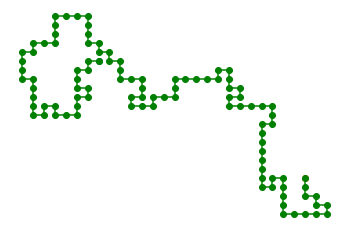
\includegraphics[width=0.45\textwidth]{../images/loose_conf.png}
	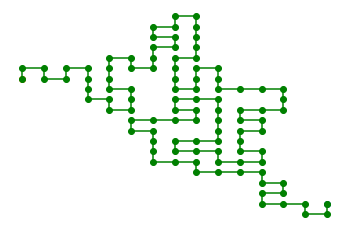
\includegraphics[width=0.45\textwidth]{../images/dense_conf.png} 
	\caption{Пример неплотной и плотной конформации}
\end{figure}

Если посмотреть на изображения конформаций каждого вида, хорошо видно, что плотные конформации по структуре близки с двумерным решёткам, где у каждого узла имеется множество соседей, и развёрнутые конформации наоборот близки к одномерным структурам, где узлы у которых больше 2 соседей встречаются редко. Соответственно можно предположить, что плотные конформации будут иметь свойства схожие с двумерными решётками, а развёрнутые с одномерными.


\subsection{Модель изинга}
Будем рассматривать конформацю как модель Изинга. В каждом узле конформации размещён спин $s_i$ принимающий значения $+1, -1$. Внешнее поле отсутствует. Гамильтониан системы $H = -J\sum_{i, j} s_i s_j$ где $i, j$ индексы соседних узлов, $J$ - коэффициент взаимодействия.

\subsection{Метод Монте-Карло}
Для моделирования системы используется метод Монте-Карло. Мною были реализованы версии с односпиновым и кластернным апдейтом, однако для измерений я использовал кластерную версию. Благодаря отказоустойчивости она работает значительно быстрее, и быстрее сходится, особенно при низких температурах.

На каждой итерации мы выбираем случайный спин и начиная с него начинаем строить кластер из одинаково направленных спинов, добавляя новые спины в кластер с определённой вероятностью. затем мы меняем значения спинов в кластере на противоположные.

\section{Алгоритмы}

Реализованы два алгоритма обновления спинов. Односпиновый и кластерный апдейт. Оба алгоритма работают на произвольном графе, используя таблицу соседей. Алгоритмы реализованы как отдельные библиотеки для Python, и написаны с использованием технологии Cython для ускорения работы. Кластерный апдейт является более эффективным по времени работы и количеству шагов, которые необходимо выполнить для хорошей сходимости модели.

\subsection{Проверка алгоритмов}

Чтобы убедиться что алгоритмы работают правильно мы проверили, что оба алгоритма дают одинаковые результаты на одних и тех же конформациях, так же сравнил их с точными решениями для одномерной модели Изинга.

Результаты замеров кластерным и односпиновым апдейтом совпадают в пределах погрешности.

\begin{figure}[H]
	\centering
	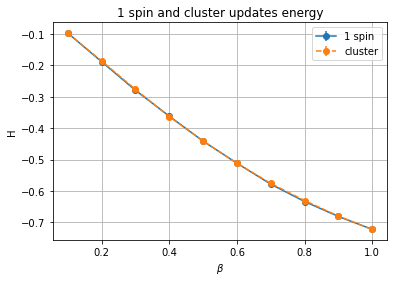
\includegraphics[width = 0.45\textwidth]{../images/1spin_&_cluster_ene.png} 
	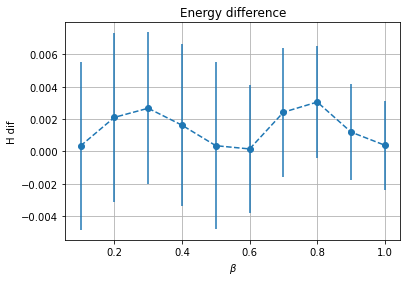
\includegraphics[width = 0.45\textwidth]{../images/1spin_&_cluster_ene_dif.png} 
	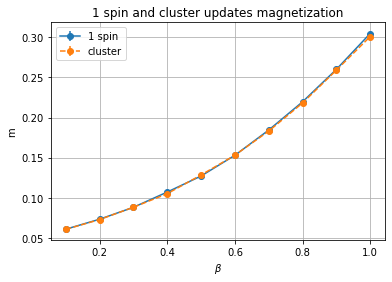
\includegraphics[width = 0.45\textwidth]{../images/1spin_&_cluster_mag.png} 
	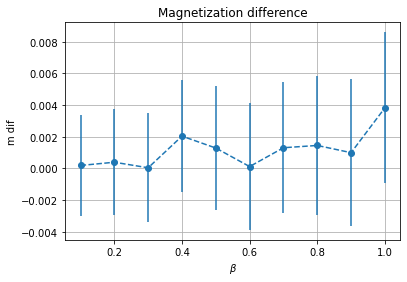
\includegraphics[width = 0.45\textwidth]{../images/1spin_&_cluster_mag_dif.png} 
	%% add magnetization
	\caption{кластерный и односпиновый апдейт}
\end{figure}

Для сравнения с точными значениями для одномерной модели Изинга, мы используем замкнутый квадратный контур. Данная конформация по свойствам полностью совпадает с одномерной моделью Изинга с открытыми граничными условиями.

\begin{figure}[H]
	\centering
	\begin{subfigure}[t]{0.45\textwidth}
		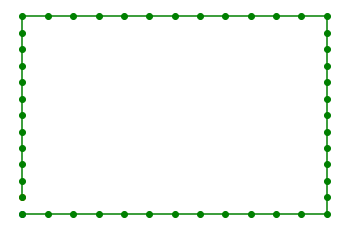
\includegraphics[width = \textwidth]{../images/1D_conf.png} 
		\caption{Конформация эмитирующая одномерную модель}
	\end{subfigure}
	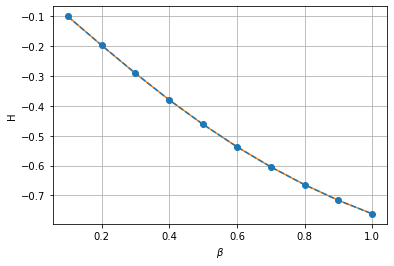
\includegraphics[width = 0.45\textwidth]{../images/1D_ene.png}
	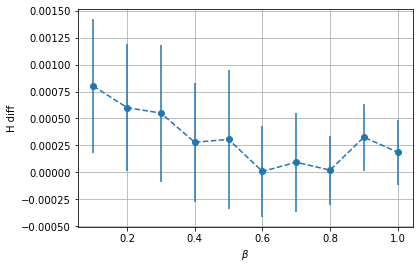
\includegraphics[width = 0.45\textwidth]{../images/1D_ene_diff.png} 
	%% add magnetization
	\caption{Сравнение с точным решением одномерной модели}
\end{figure}

Так же был написан код, точно вычисляющий энергию системы путём полного перебора всех её состояний. Сравнение на маленьких конформациях (длина 10) даёт одинаковые результаты.

%TODO втавить результаты поного перебора

Примеры с использованием кластерного апдейта добавлены в библиотеку \texttt{mc\_lib}.

%\section{Конформации при низких температурах}
До этого мы рассматривали только конформации полученные при низких температурах, где мы хотим определить точку перехода. Другая часть этого исследования заключается в проверке того, что у конформаций, полученных при низкой температуре, магнитный фазовый переход не отсутствует.

Для этого были cгенерированы 4 набора конформаций с длинами 250, 500, 1000, 2000 по 1000 конформаций в каждом наборе. Как и ожидалось средняя намагниченность по конформациям значительно меньше, чем у конформаций при $U = 1$(сравнение на Рис. \ref{fig:U0.1_mean_mag2}).

\begin{figure}[htb]
	\centering
	%% Creator: Matplotlib, PGF backend
%%
%% To include the figure in your LaTeX document, write
%%   \input{<filename>.pgf}
%%
%% Make sure the required packages are loaded in your preamble
%%   \usepackage{pgf}
%%
%% Also ensure that all the required font packages are loaded; for instance,
%% the lmodern package is sometimes necessary when using math font.
%%   \usepackage{lmodern}
%%
%% Figures using additional raster images can only be included by \input if
%% they are in the same directory as the main LaTeX file. For loading figures
%% from other directories you can use the `import` package
%%   \usepackage{import}
%%
%% and then include the figures with
%%   \import{<path to file>}{<filename>.pgf}
%%
%% Matplotlib used the following preamble
%%   
%%   \makeatletter\@ifpackageloaded{underscore}{}{\usepackage[strings]{underscore}}\makeatother
%%
\begingroup%
\makeatletter%
\begin{pgfpicture}%
\pgfpathrectangle{\pgfpointorigin}{\pgfqpoint{4.353372in}{2.871460in}}%
\pgfusepath{use as bounding box, clip}%
\begin{pgfscope}%
\pgfsetbuttcap%
\pgfsetmiterjoin%
\definecolor{currentfill}{rgb}{1.000000,1.000000,1.000000}%
\pgfsetfillcolor{currentfill}%
\pgfsetlinewidth{0.000000pt}%
\definecolor{currentstroke}{rgb}{1.000000,1.000000,1.000000}%
\pgfsetstrokecolor{currentstroke}%
\pgfsetdash{}{0pt}%
\pgfpathmoveto{\pgfqpoint{0.000000in}{0.000000in}}%
\pgfpathlineto{\pgfqpoint{4.353372in}{0.000000in}}%
\pgfpathlineto{\pgfqpoint{4.353372in}{2.871460in}}%
\pgfpathlineto{\pgfqpoint{0.000000in}{2.871460in}}%
\pgfpathlineto{\pgfqpoint{0.000000in}{0.000000in}}%
\pgfpathclose%
\pgfusepath{fill}%
\end{pgfscope}%
\begin{pgfscope}%
\pgfsetbuttcap%
\pgfsetmiterjoin%
\definecolor{currentfill}{rgb}{1.000000,1.000000,1.000000}%
\pgfsetfillcolor{currentfill}%
\pgfsetlinewidth{0.000000pt}%
\definecolor{currentstroke}{rgb}{0.000000,0.000000,0.000000}%
\pgfsetstrokecolor{currentstroke}%
\pgfsetstrokeopacity{0.000000}%
\pgfsetdash{}{0pt}%
\pgfpathmoveto{\pgfqpoint{0.553704in}{0.499691in}}%
\pgfpathlineto{\pgfqpoint{4.253372in}{0.499691in}}%
\pgfpathlineto{\pgfqpoint{4.253372in}{2.771460in}}%
\pgfpathlineto{\pgfqpoint{0.553704in}{2.771460in}}%
\pgfpathlineto{\pgfqpoint{0.553704in}{0.499691in}}%
\pgfpathclose%
\pgfusepath{fill}%
\end{pgfscope}%
\begin{pgfscope}%
\pgfpathrectangle{\pgfqpoint{0.553704in}{0.499691in}}{\pgfqpoint{3.699668in}{2.271769in}}%
\pgfusepath{clip}%
\pgfsetrectcap%
\pgfsetroundjoin%
\pgfsetlinewidth{0.803000pt}%
\definecolor{currentstroke}{rgb}{0.690196,0.690196,0.690196}%
\pgfsetstrokecolor{currentstroke}%
\pgfsetdash{}{0pt}%
\pgfpathmoveto{\pgfqpoint{1.102801in}{0.499691in}}%
\pgfpathlineto{\pgfqpoint{1.102801in}{2.771460in}}%
\pgfusepath{stroke}%
\end{pgfscope}%
\begin{pgfscope}%
\pgfsetbuttcap%
\pgfsetroundjoin%
\definecolor{currentfill}{rgb}{0.000000,0.000000,0.000000}%
\pgfsetfillcolor{currentfill}%
\pgfsetlinewidth{0.803000pt}%
\definecolor{currentstroke}{rgb}{0.000000,0.000000,0.000000}%
\pgfsetstrokecolor{currentstroke}%
\pgfsetdash{}{0pt}%
\pgfsys@defobject{currentmarker}{\pgfqpoint{0.000000in}{-0.048611in}}{\pgfqpoint{0.000000in}{0.000000in}}{%
\pgfpathmoveto{\pgfqpoint{0.000000in}{0.000000in}}%
\pgfpathlineto{\pgfqpoint{0.000000in}{-0.048611in}}%
\pgfusepath{stroke,fill}%
}%
\begin{pgfscope}%
\pgfsys@transformshift{1.102801in}{0.499691in}%
\pgfsys@useobject{currentmarker}{}%
\end{pgfscope}%
\end{pgfscope}%
\begin{pgfscope}%
\definecolor{textcolor}{rgb}{0.000000,0.000000,0.000000}%
\pgfsetstrokecolor{textcolor}%
\pgfsetfillcolor{textcolor}%
\pgftext[x=1.102801in,y=0.402469in,,top]{\color{textcolor}\sffamily\fontsize{10.000000}{12.000000}\selectfont 0.2}%
\end{pgfscope}%
\begin{pgfscope}%
\pgfpathrectangle{\pgfqpoint{0.553704in}{0.499691in}}{\pgfqpoint{3.699668in}{2.271769in}}%
\pgfusepath{clip}%
\pgfsetrectcap%
\pgfsetroundjoin%
\pgfsetlinewidth{0.803000pt}%
\definecolor{currentstroke}{rgb}{0.690196,0.690196,0.690196}%
\pgfsetstrokecolor{currentstroke}%
\pgfsetdash{}{0pt}%
\pgfpathmoveto{\pgfqpoint{1.846079in}{0.499691in}}%
\pgfpathlineto{\pgfqpoint{1.846079in}{2.771460in}}%
\pgfusepath{stroke}%
\end{pgfscope}%
\begin{pgfscope}%
\pgfsetbuttcap%
\pgfsetroundjoin%
\definecolor{currentfill}{rgb}{0.000000,0.000000,0.000000}%
\pgfsetfillcolor{currentfill}%
\pgfsetlinewidth{0.803000pt}%
\definecolor{currentstroke}{rgb}{0.000000,0.000000,0.000000}%
\pgfsetstrokecolor{currentstroke}%
\pgfsetdash{}{0pt}%
\pgfsys@defobject{currentmarker}{\pgfqpoint{0.000000in}{-0.048611in}}{\pgfqpoint{0.000000in}{0.000000in}}{%
\pgfpathmoveto{\pgfqpoint{0.000000in}{0.000000in}}%
\pgfpathlineto{\pgfqpoint{0.000000in}{-0.048611in}}%
\pgfusepath{stroke,fill}%
}%
\begin{pgfscope}%
\pgfsys@transformshift{1.846079in}{0.499691in}%
\pgfsys@useobject{currentmarker}{}%
\end{pgfscope}%
\end{pgfscope}%
\begin{pgfscope}%
\definecolor{textcolor}{rgb}{0.000000,0.000000,0.000000}%
\pgfsetstrokecolor{textcolor}%
\pgfsetfillcolor{textcolor}%
\pgftext[x=1.846079in,y=0.402469in,,top]{\color{textcolor}\sffamily\fontsize{10.000000}{12.000000}\selectfont 0.4}%
\end{pgfscope}%
\begin{pgfscope}%
\pgfpathrectangle{\pgfqpoint{0.553704in}{0.499691in}}{\pgfqpoint{3.699668in}{2.271769in}}%
\pgfusepath{clip}%
\pgfsetrectcap%
\pgfsetroundjoin%
\pgfsetlinewidth{0.803000pt}%
\definecolor{currentstroke}{rgb}{0.690196,0.690196,0.690196}%
\pgfsetstrokecolor{currentstroke}%
\pgfsetdash{}{0pt}%
\pgfpathmoveto{\pgfqpoint{2.589358in}{0.499691in}}%
\pgfpathlineto{\pgfqpoint{2.589358in}{2.771460in}}%
\pgfusepath{stroke}%
\end{pgfscope}%
\begin{pgfscope}%
\pgfsetbuttcap%
\pgfsetroundjoin%
\definecolor{currentfill}{rgb}{0.000000,0.000000,0.000000}%
\pgfsetfillcolor{currentfill}%
\pgfsetlinewidth{0.803000pt}%
\definecolor{currentstroke}{rgb}{0.000000,0.000000,0.000000}%
\pgfsetstrokecolor{currentstroke}%
\pgfsetdash{}{0pt}%
\pgfsys@defobject{currentmarker}{\pgfqpoint{0.000000in}{-0.048611in}}{\pgfqpoint{0.000000in}{0.000000in}}{%
\pgfpathmoveto{\pgfqpoint{0.000000in}{0.000000in}}%
\pgfpathlineto{\pgfqpoint{0.000000in}{-0.048611in}}%
\pgfusepath{stroke,fill}%
}%
\begin{pgfscope}%
\pgfsys@transformshift{2.589358in}{0.499691in}%
\pgfsys@useobject{currentmarker}{}%
\end{pgfscope}%
\end{pgfscope}%
\begin{pgfscope}%
\definecolor{textcolor}{rgb}{0.000000,0.000000,0.000000}%
\pgfsetstrokecolor{textcolor}%
\pgfsetfillcolor{textcolor}%
\pgftext[x=2.589358in,y=0.402469in,,top]{\color{textcolor}\sffamily\fontsize{10.000000}{12.000000}\selectfont 0.6}%
\end{pgfscope}%
\begin{pgfscope}%
\pgfpathrectangle{\pgfqpoint{0.553704in}{0.499691in}}{\pgfqpoint{3.699668in}{2.271769in}}%
\pgfusepath{clip}%
\pgfsetrectcap%
\pgfsetroundjoin%
\pgfsetlinewidth{0.803000pt}%
\definecolor{currentstroke}{rgb}{0.690196,0.690196,0.690196}%
\pgfsetstrokecolor{currentstroke}%
\pgfsetdash{}{0pt}%
\pgfpathmoveto{\pgfqpoint{3.332636in}{0.499691in}}%
\pgfpathlineto{\pgfqpoint{3.332636in}{2.771460in}}%
\pgfusepath{stroke}%
\end{pgfscope}%
\begin{pgfscope}%
\pgfsetbuttcap%
\pgfsetroundjoin%
\definecolor{currentfill}{rgb}{0.000000,0.000000,0.000000}%
\pgfsetfillcolor{currentfill}%
\pgfsetlinewidth{0.803000pt}%
\definecolor{currentstroke}{rgb}{0.000000,0.000000,0.000000}%
\pgfsetstrokecolor{currentstroke}%
\pgfsetdash{}{0pt}%
\pgfsys@defobject{currentmarker}{\pgfqpoint{0.000000in}{-0.048611in}}{\pgfqpoint{0.000000in}{0.000000in}}{%
\pgfpathmoveto{\pgfqpoint{0.000000in}{0.000000in}}%
\pgfpathlineto{\pgfqpoint{0.000000in}{-0.048611in}}%
\pgfusepath{stroke,fill}%
}%
\begin{pgfscope}%
\pgfsys@transformshift{3.332636in}{0.499691in}%
\pgfsys@useobject{currentmarker}{}%
\end{pgfscope}%
\end{pgfscope}%
\begin{pgfscope}%
\definecolor{textcolor}{rgb}{0.000000,0.000000,0.000000}%
\pgfsetstrokecolor{textcolor}%
\pgfsetfillcolor{textcolor}%
\pgftext[x=3.332636in,y=0.402469in,,top]{\color{textcolor}\sffamily\fontsize{10.000000}{12.000000}\selectfont 0.8}%
\end{pgfscope}%
\begin{pgfscope}%
\pgfpathrectangle{\pgfqpoint{0.553704in}{0.499691in}}{\pgfqpoint{3.699668in}{2.271769in}}%
\pgfusepath{clip}%
\pgfsetrectcap%
\pgfsetroundjoin%
\pgfsetlinewidth{0.803000pt}%
\definecolor{currentstroke}{rgb}{0.690196,0.690196,0.690196}%
\pgfsetstrokecolor{currentstroke}%
\pgfsetdash{}{0pt}%
\pgfpathmoveto{\pgfqpoint{4.075914in}{0.499691in}}%
\pgfpathlineto{\pgfqpoint{4.075914in}{2.771460in}}%
\pgfusepath{stroke}%
\end{pgfscope}%
\begin{pgfscope}%
\pgfsetbuttcap%
\pgfsetroundjoin%
\definecolor{currentfill}{rgb}{0.000000,0.000000,0.000000}%
\pgfsetfillcolor{currentfill}%
\pgfsetlinewidth{0.803000pt}%
\definecolor{currentstroke}{rgb}{0.000000,0.000000,0.000000}%
\pgfsetstrokecolor{currentstroke}%
\pgfsetdash{}{0pt}%
\pgfsys@defobject{currentmarker}{\pgfqpoint{0.000000in}{-0.048611in}}{\pgfqpoint{0.000000in}{0.000000in}}{%
\pgfpathmoveto{\pgfqpoint{0.000000in}{0.000000in}}%
\pgfpathlineto{\pgfqpoint{0.000000in}{-0.048611in}}%
\pgfusepath{stroke,fill}%
}%
\begin{pgfscope}%
\pgfsys@transformshift{4.075914in}{0.499691in}%
\pgfsys@useobject{currentmarker}{}%
\end{pgfscope}%
\end{pgfscope}%
\begin{pgfscope}%
\definecolor{textcolor}{rgb}{0.000000,0.000000,0.000000}%
\pgfsetstrokecolor{textcolor}%
\pgfsetfillcolor{textcolor}%
\pgftext[x=4.075914in,y=0.402469in,,top]{\color{textcolor}\sffamily\fontsize{10.000000}{12.000000}\selectfont 1.0}%
\end{pgfscope}%
\begin{pgfscope}%
\definecolor{textcolor}{rgb}{0.000000,0.000000,0.000000}%
\pgfsetstrokecolor{textcolor}%
\pgfsetfillcolor{textcolor}%
\pgftext[x=2.403538in,y=0.223457in,,top]{\color{textcolor}\sffamily\fontsize{10.000000}{12.000000}\selectfont \(\displaystyle \beta\)}%
\end{pgfscope}%
\begin{pgfscope}%
\pgfpathrectangle{\pgfqpoint{0.553704in}{0.499691in}}{\pgfqpoint{3.699668in}{2.271769in}}%
\pgfusepath{clip}%
\pgfsetrectcap%
\pgfsetroundjoin%
\pgfsetlinewidth{0.803000pt}%
\definecolor{currentstroke}{rgb}{0.690196,0.690196,0.690196}%
\pgfsetstrokecolor{currentstroke}%
\pgfsetdash{}{0pt}%
\pgfpathmoveto{\pgfqpoint{0.553704in}{0.747434in}}%
\pgfpathlineto{\pgfqpoint{4.253372in}{0.747434in}}%
\pgfusepath{stroke}%
\end{pgfscope}%
\begin{pgfscope}%
\pgfsetbuttcap%
\pgfsetroundjoin%
\definecolor{currentfill}{rgb}{0.000000,0.000000,0.000000}%
\pgfsetfillcolor{currentfill}%
\pgfsetlinewidth{0.803000pt}%
\definecolor{currentstroke}{rgb}{0.000000,0.000000,0.000000}%
\pgfsetstrokecolor{currentstroke}%
\pgfsetdash{}{0pt}%
\pgfsys@defobject{currentmarker}{\pgfqpoint{-0.048611in}{0.000000in}}{\pgfqpoint{-0.000000in}{0.000000in}}{%
\pgfpathmoveto{\pgfqpoint{-0.000000in}{0.000000in}}%
\pgfpathlineto{\pgfqpoint{-0.048611in}{0.000000in}}%
\pgfusepath{stroke,fill}%
}%
\begin{pgfscope}%
\pgfsys@transformshift{0.553704in}{0.747434in}%
\pgfsys@useobject{currentmarker}{}%
\end{pgfscope}%
\end{pgfscope}%
\begin{pgfscope}%
\definecolor{textcolor}{rgb}{0.000000,0.000000,0.000000}%
\pgfsetstrokecolor{textcolor}%
\pgfsetfillcolor{textcolor}%
\pgftext[x=0.279012in, y=0.699208in, left, base]{\color{textcolor}\sffamily\fontsize{10.000000}{12.000000}\selectfont 0.0}%
\end{pgfscope}%
\begin{pgfscope}%
\pgfpathrectangle{\pgfqpoint{0.553704in}{0.499691in}}{\pgfqpoint{3.699668in}{2.271769in}}%
\pgfusepath{clip}%
\pgfsetrectcap%
\pgfsetroundjoin%
\pgfsetlinewidth{0.803000pt}%
\definecolor{currentstroke}{rgb}{0.690196,0.690196,0.690196}%
\pgfsetstrokecolor{currentstroke}%
\pgfsetdash{}{0pt}%
\pgfpathmoveto{\pgfqpoint{0.553704in}{1.274009in}}%
\pgfpathlineto{\pgfqpoint{4.253372in}{1.274009in}}%
\pgfusepath{stroke}%
\end{pgfscope}%
\begin{pgfscope}%
\pgfsetbuttcap%
\pgfsetroundjoin%
\definecolor{currentfill}{rgb}{0.000000,0.000000,0.000000}%
\pgfsetfillcolor{currentfill}%
\pgfsetlinewidth{0.803000pt}%
\definecolor{currentstroke}{rgb}{0.000000,0.000000,0.000000}%
\pgfsetstrokecolor{currentstroke}%
\pgfsetdash{}{0pt}%
\pgfsys@defobject{currentmarker}{\pgfqpoint{-0.048611in}{0.000000in}}{\pgfqpoint{-0.000000in}{0.000000in}}{%
\pgfpathmoveto{\pgfqpoint{-0.000000in}{0.000000in}}%
\pgfpathlineto{\pgfqpoint{-0.048611in}{0.000000in}}%
\pgfusepath{stroke,fill}%
}%
\begin{pgfscope}%
\pgfsys@transformshift{0.553704in}{1.274009in}%
\pgfsys@useobject{currentmarker}{}%
\end{pgfscope}%
\end{pgfscope}%
\begin{pgfscope}%
\definecolor{textcolor}{rgb}{0.000000,0.000000,0.000000}%
\pgfsetstrokecolor{textcolor}%
\pgfsetfillcolor{textcolor}%
\pgftext[x=0.279012in, y=1.225783in, left, base]{\color{textcolor}\sffamily\fontsize{10.000000}{12.000000}\selectfont 0.2}%
\end{pgfscope}%
\begin{pgfscope}%
\pgfpathrectangle{\pgfqpoint{0.553704in}{0.499691in}}{\pgfqpoint{3.699668in}{2.271769in}}%
\pgfusepath{clip}%
\pgfsetrectcap%
\pgfsetroundjoin%
\pgfsetlinewidth{0.803000pt}%
\definecolor{currentstroke}{rgb}{0.690196,0.690196,0.690196}%
\pgfsetstrokecolor{currentstroke}%
\pgfsetdash{}{0pt}%
\pgfpathmoveto{\pgfqpoint{0.553704in}{1.800584in}}%
\pgfpathlineto{\pgfqpoint{4.253372in}{1.800584in}}%
\pgfusepath{stroke}%
\end{pgfscope}%
\begin{pgfscope}%
\pgfsetbuttcap%
\pgfsetroundjoin%
\definecolor{currentfill}{rgb}{0.000000,0.000000,0.000000}%
\pgfsetfillcolor{currentfill}%
\pgfsetlinewidth{0.803000pt}%
\definecolor{currentstroke}{rgb}{0.000000,0.000000,0.000000}%
\pgfsetstrokecolor{currentstroke}%
\pgfsetdash{}{0pt}%
\pgfsys@defobject{currentmarker}{\pgfqpoint{-0.048611in}{0.000000in}}{\pgfqpoint{-0.000000in}{0.000000in}}{%
\pgfpathmoveto{\pgfqpoint{-0.000000in}{0.000000in}}%
\pgfpathlineto{\pgfqpoint{-0.048611in}{0.000000in}}%
\pgfusepath{stroke,fill}%
}%
\begin{pgfscope}%
\pgfsys@transformshift{0.553704in}{1.800584in}%
\pgfsys@useobject{currentmarker}{}%
\end{pgfscope}%
\end{pgfscope}%
\begin{pgfscope}%
\definecolor{textcolor}{rgb}{0.000000,0.000000,0.000000}%
\pgfsetstrokecolor{textcolor}%
\pgfsetfillcolor{textcolor}%
\pgftext[x=0.279012in, y=1.752358in, left, base]{\color{textcolor}\sffamily\fontsize{10.000000}{12.000000}\selectfont 0.4}%
\end{pgfscope}%
\begin{pgfscope}%
\pgfpathrectangle{\pgfqpoint{0.553704in}{0.499691in}}{\pgfqpoint{3.699668in}{2.271769in}}%
\pgfusepath{clip}%
\pgfsetrectcap%
\pgfsetroundjoin%
\pgfsetlinewidth{0.803000pt}%
\definecolor{currentstroke}{rgb}{0.690196,0.690196,0.690196}%
\pgfsetstrokecolor{currentstroke}%
\pgfsetdash{}{0pt}%
\pgfpathmoveto{\pgfqpoint{0.553704in}{2.327159in}}%
\pgfpathlineto{\pgfqpoint{4.253372in}{2.327159in}}%
\pgfusepath{stroke}%
\end{pgfscope}%
\begin{pgfscope}%
\pgfsetbuttcap%
\pgfsetroundjoin%
\definecolor{currentfill}{rgb}{0.000000,0.000000,0.000000}%
\pgfsetfillcolor{currentfill}%
\pgfsetlinewidth{0.803000pt}%
\definecolor{currentstroke}{rgb}{0.000000,0.000000,0.000000}%
\pgfsetstrokecolor{currentstroke}%
\pgfsetdash{}{0pt}%
\pgfsys@defobject{currentmarker}{\pgfqpoint{-0.048611in}{0.000000in}}{\pgfqpoint{-0.000000in}{0.000000in}}{%
\pgfpathmoveto{\pgfqpoint{-0.000000in}{0.000000in}}%
\pgfpathlineto{\pgfqpoint{-0.048611in}{0.000000in}}%
\pgfusepath{stroke,fill}%
}%
\begin{pgfscope}%
\pgfsys@transformshift{0.553704in}{2.327159in}%
\pgfsys@useobject{currentmarker}{}%
\end{pgfscope}%
\end{pgfscope}%
\begin{pgfscope}%
\definecolor{textcolor}{rgb}{0.000000,0.000000,0.000000}%
\pgfsetstrokecolor{textcolor}%
\pgfsetfillcolor{textcolor}%
\pgftext[x=0.279012in, y=2.278933in, left, base]{\color{textcolor}\sffamily\fontsize{10.000000}{12.000000}\selectfont 0.6}%
\end{pgfscope}%
\begin{pgfscope}%
\definecolor{textcolor}{rgb}{0.000000,0.000000,0.000000}%
\pgfsetstrokecolor{textcolor}%
\pgfsetfillcolor{textcolor}%
\pgftext[x=0.223457in,y=1.635575in,,bottom,rotate=90.000000]{\color{textcolor}\sffamily\fontsize{10.000000}{12.000000}\selectfont \(\displaystyle M^2\)}%
\end{pgfscope}%
\begin{pgfscope}%
\pgfpathrectangle{\pgfqpoint{0.553704in}{0.499691in}}{\pgfqpoint{3.699668in}{2.271769in}}%
\pgfusepath{clip}%
\pgfsetbuttcap%
\pgfsetroundjoin%
\pgfsetlinewidth{1.505625pt}%
\definecolor{currentstroke}{rgb}{0.121569,0.466667,0.705882}%
\pgfsetstrokecolor{currentstroke}%
\pgfsetdash{}{0pt}%
\pgfpathmoveto{\pgfqpoint{0.721871in}{0.760549in}}%
\pgfpathlineto{\pgfqpoint{0.721871in}{0.761740in}}%
\pgfusepath{stroke}%
\end{pgfscope}%
\begin{pgfscope}%
\pgfpathrectangle{\pgfqpoint{0.553704in}{0.499691in}}{\pgfqpoint{3.699668in}{2.271769in}}%
\pgfusepath{clip}%
\pgfsetbuttcap%
\pgfsetroundjoin%
\pgfsetlinewidth{1.505625pt}%
\definecolor{currentstroke}{rgb}{0.121569,0.466667,0.705882}%
\pgfsetstrokecolor{currentstroke}%
\pgfsetdash{}{0pt}%
\pgfpathmoveto{\pgfqpoint{1.093510in}{0.764153in}}%
\pgfpathlineto{\pgfqpoint{1.093510in}{0.767878in}}%
\pgfusepath{stroke}%
\end{pgfscope}%
\begin{pgfscope}%
\pgfpathrectangle{\pgfqpoint{0.553704in}{0.499691in}}{\pgfqpoint{3.699668in}{2.271769in}}%
\pgfusepath{clip}%
\pgfsetbuttcap%
\pgfsetroundjoin%
\pgfsetlinewidth{1.505625pt}%
\definecolor{currentstroke}{rgb}{0.121569,0.466667,0.705882}%
\pgfsetstrokecolor{currentstroke}%
\pgfsetdash{}{0pt}%
\pgfpathmoveto{\pgfqpoint{1.465149in}{0.768371in}}%
\pgfpathlineto{\pgfqpoint{1.465149in}{0.779693in}}%
\pgfusepath{stroke}%
\end{pgfscope}%
\begin{pgfscope}%
\pgfpathrectangle{\pgfqpoint{0.553704in}{0.499691in}}{\pgfqpoint{3.699668in}{2.271769in}}%
\pgfusepath{clip}%
\pgfsetbuttcap%
\pgfsetroundjoin%
\pgfsetlinewidth{1.505625pt}%
\definecolor{currentstroke}{rgb}{0.121569,0.466667,0.705882}%
\pgfsetstrokecolor{currentstroke}%
\pgfsetdash{}{0pt}%
\pgfpathmoveto{\pgfqpoint{1.836788in}{0.770978in}}%
\pgfpathlineto{\pgfqpoint{1.836788in}{0.807845in}}%
\pgfusepath{stroke}%
\end{pgfscope}%
\begin{pgfscope}%
\pgfpathrectangle{\pgfqpoint{0.553704in}{0.499691in}}{\pgfqpoint{3.699668in}{2.271769in}}%
\pgfusepath{clip}%
\pgfsetbuttcap%
\pgfsetroundjoin%
\pgfsetlinewidth{1.505625pt}%
\definecolor{currentstroke}{rgb}{0.121569,0.466667,0.705882}%
\pgfsetstrokecolor{currentstroke}%
\pgfsetdash{}{0pt}%
\pgfpathmoveto{\pgfqpoint{2.208428in}{0.758303in}}%
\pgfpathlineto{\pgfqpoint{2.208428in}{0.888628in}}%
\pgfusepath{stroke}%
\end{pgfscope}%
\begin{pgfscope}%
\pgfpathrectangle{\pgfqpoint{0.553704in}{0.499691in}}{\pgfqpoint{3.699668in}{2.271769in}}%
\pgfusepath{clip}%
\pgfsetbuttcap%
\pgfsetroundjoin%
\pgfsetlinewidth{1.505625pt}%
\definecolor{currentstroke}{rgb}{0.121569,0.466667,0.705882}%
\pgfsetstrokecolor{currentstroke}%
\pgfsetdash{}{0pt}%
\pgfpathmoveto{\pgfqpoint{2.580067in}{0.719644in}}%
\pgfpathlineto{\pgfqpoint{2.580067in}{1.050782in}}%
\pgfusepath{stroke}%
\end{pgfscope}%
\begin{pgfscope}%
\pgfpathrectangle{\pgfqpoint{0.553704in}{0.499691in}}{\pgfqpoint{3.699668in}{2.271769in}}%
\pgfusepath{clip}%
\pgfsetbuttcap%
\pgfsetroundjoin%
\pgfsetlinewidth{1.505625pt}%
\definecolor{currentstroke}{rgb}{0.121569,0.466667,0.705882}%
\pgfsetstrokecolor{currentstroke}%
\pgfsetdash{}{0pt}%
\pgfpathmoveto{\pgfqpoint{2.951706in}{0.683333in}}%
\pgfpathlineto{\pgfqpoint{2.951706in}{1.233252in}}%
\pgfusepath{stroke}%
\end{pgfscope}%
\begin{pgfscope}%
\pgfpathrectangle{\pgfqpoint{0.553704in}{0.499691in}}{\pgfqpoint{3.699668in}{2.271769in}}%
\pgfusepath{clip}%
\pgfsetbuttcap%
\pgfsetroundjoin%
\pgfsetlinewidth{1.505625pt}%
\definecolor{currentstroke}{rgb}{0.121569,0.466667,0.705882}%
\pgfsetstrokecolor{currentstroke}%
\pgfsetdash{}{0pt}%
\pgfpathmoveto{\pgfqpoint{3.323345in}{0.666644in}}%
\pgfpathlineto{\pgfqpoint{3.323345in}{1.390987in}}%
\pgfusepath{stroke}%
\end{pgfscope}%
\begin{pgfscope}%
\pgfpathrectangle{\pgfqpoint{0.553704in}{0.499691in}}{\pgfqpoint{3.699668in}{2.271769in}}%
\pgfusepath{clip}%
\pgfsetbuttcap%
\pgfsetroundjoin%
\pgfsetlinewidth{1.505625pt}%
\definecolor{currentstroke}{rgb}{0.121569,0.466667,0.705882}%
\pgfsetstrokecolor{currentstroke}%
\pgfsetdash{}{0pt}%
\pgfpathmoveto{\pgfqpoint{3.694984in}{0.665905in}}%
\pgfpathlineto{\pgfqpoint{3.694984in}{1.524878in}}%
\pgfusepath{stroke}%
\end{pgfscope}%
\begin{pgfscope}%
\pgfpathrectangle{\pgfqpoint{0.553704in}{0.499691in}}{\pgfqpoint{3.699668in}{2.271769in}}%
\pgfusepath{clip}%
\pgfsetbuttcap%
\pgfsetroundjoin%
\pgfsetlinewidth{1.505625pt}%
\definecolor{currentstroke}{rgb}{0.121569,0.466667,0.705882}%
\pgfsetstrokecolor{currentstroke}%
\pgfsetdash{}{0pt}%
\pgfpathmoveto{\pgfqpoint{4.066623in}{0.677349in}}%
\pgfpathlineto{\pgfqpoint{4.066623in}{1.643496in}}%
\pgfusepath{stroke}%
\end{pgfscope}%
\begin{pgfscope}%
\pgfpathrectangle{\pgfqpoint{0.553704in}{0.499691in}}{\pgfqpoint{3.699668in}{2.271769in}}%
\pgfusepath{clip}%
\pgfsetbuttcap%
\pgfsetroundjoin%
\pgfsetlinewidth{1.505625pt}%
\definecolor{currentstroke}{rgb}{1.000000,0.498039,0.054902}%
\pgfsetstrokecolor{currentstroke}%
\pgfsetdash{}{0pt}%
\pgfpathmoveto{\pgfqpoint{0.731162in}{0.750680in}}%
\pgfpathlineto{\pgfqpoint{0.731162in}{0.751145in}}%
\pgfusepath{stroke}%
\end{pgfscope}%
\begin{pgfscope}%
\pgfpathrectangle{\pgfqpoint{0.553704in}{0.499691in}}{\pgfqpoint{3.699668in}{2.271769in}}%
\pgfusepath{clip}%
\pgfsetbuttcap%
\pgfsetroundjoin%
\pgfsetlinewidth{1.505625pt}%
\definecolor{currentstroke}{rgb}{1.000000,0.498039,0.054902}%
\pgfsetstrokecolor{currentstroke}%
\pgfsetdash{}{0pt}%
\pgfpathmoveto{\pgfqpoint{1.102801in}{0.751640in}}%
\pgfpathlineto{\pgfqpoint{1.102801in}{0.752866in}}%
\pgfusepath{stroke}%
\end{pgfscope}%
\begin{pgfscope}%
\pgfpathrectangle{\pgfqpoint{0.553704in}{0.499691in}}{\pgfqpoint{3.699668in}{2.271769in}}%
\pgfusepath{clip}%
\pgfsetbuttcap%
\pgfsetroundjoin%
\pgfsetlinewidth{1.505625pt}%
\definecolor{currentstroke}{rgb}{1.000000,0.498039,0.054902}%
\pgfsetstrokecolor{currentstroke}%
\pgfsetdash{}{0pt}%
\pgfpathmoveto{\pgfqpoint{1.474440in}{0.752699in}}%
\pgfpathlineto{\pgfqpoint{1.474440in}{0.756521in}}%
\pgfusepath{stroke}%
\end{pgfscope}%
\begin{pgfscope}%
\pgfpathrectangle{\pgfqpoint{0.553704in}{0.499691in}}{\pgfqpoint{3.699668in}{2.271769in}}%
\pgfusepath{clip}%
\pgfsetbuttcap%
\pgfsetroundjoin%
\pgfsetlinewidth{1.505625pt}%
\definecolor{currentstroke}{rgb}{1.000000,0.498039,0.054902}%
\pgfsetstrokecolor{currentstroke}%
\pgfsetdash{}{0pt}%
\pgfpathmoveto{\pgfqpoint{1.846079in}{0.752930in}}%
\pgfpathlineto{\pgfqpoint{1.846079in}{0.767666in}}%
\pgfusepath{stroke}%
\end{pgfscope}%
\begin{pgfscope}%
\pgfpathrectangle{\pgfqpoint{0.553704in}{0.499691in}}{\pgfqpoint{3.699668in}{2.271769in}}%
\pgfusepath{clip}%
\pgfsetbuttcap%
\pgfsetroundjoin%
\pgfsetlinewidth{1.505625pt}%
\definecolor{currentstroke}{rgb}{1.000000,0.498039,0.054902}%
\pgfsetstrokecolor{currentstroke}%
\pgfsetdash{}{0pt}%
\pgfpathmoveto{\pgfqpoint{2.217719in}{0.735359in}}%
\pgfpathlineto{\pgfqpoint{2.217719in}{0.829521in}}%
\pgfusepath{stroke}%
\end{pgfscope}%
\begin{pgfscope}%
\pgfpathrectangle{\pgfqpoint{0.553704in}{0.499691in}}{\pgfqpoint{3.699668in}{2.271769in}}%
\pgfusepath{clip}%
\pgfsetbuttcap%
\pgfsetroundjoin%
\pgfsetlinewidth{1.505625pt}%
\definecolor{currentstroke}{rgb}{1.000000,0.498039,0.054902}%
\pgfsetstrokecolor{currentstroke}%
\pgfsetdash{}{0pt}%
\pgfpathmoveto{\pgfqpoint{2.589358in}{0.687380in}}%
\pgfpathlineto{\pgfqpoint{2.589358in}{0.983839in}}%
\pgfusepath{stroke}%
\end{pgfscope}%
\begin{pgfscope}%
\pgfpathrectangle{\pgfqpoint{0.553704in}{0.499691in}}{\pgfqpoint{3.699668in}{2.271769in}}%
\pgfusepath{clip}%
\pgfsetbuttcap%
\pgfsetroundjoin%
\pgfsetlinewidth{1.505625pt}%
\definecolor{currentstroke}{rgb}{1.000000,0.498039,0.054902}%
\pgfsetstrokecolor{currentstroke}%
\pgfsetdash{}{0pt}%
\pgfpathmoveto{\pgfqpoint{2.960997in}{0.652628in}}%
\pgfpathlineto{\pgfqpoint{2.960997in}{1.134556in}}%
\pgfusepath{stroke}%
\end{pgfscope}%
\begin{pgfscope}%
\pgfpathrectangle{\pgfqpoint{0.553704in}{0.499691in}}{\pgfqpoint{3.699668in}{2.271769in}}%
\pgfusepath{clip}%
\pgfsetbuttcap%
\pgfsetroundjoin%
\pgfsetlinewidth{1.505625pt}%
\definecolor{currentstroke}{rgb}{1.000000,0.498039,0.054902}%
\pgfsetstrokecolor{currentstroke}%
\pgfsetdash{}{0pt}%
\pgfpathmoveto{\pgfqpoint{3.332636in}{0.629780in}}%
\pgfpathlineto{\pgfqpoint{3.332636in}{1.263651in}}%
\pgfusepath{stroke}%
\end{pgfscope}%
\begin{pgfscope}%
\pgfpathrectangle{\pgfqpoint{0.553704in}{0.499691in}}{\pgfqpoint{3.699668in}{2.271769in}}%
\pgfusepath{clip}%
\pgfsetbuttcap%
\pgfsetroundjoin%
\pgfsetlinewidth{1.505625pt}%
\definecolor{currentstroke}{rgb}{1.000000,0.498039,0.054902}%
\pgfsetstrokecolor{currentstroke}%
\pgfsetdash{}{0pt}%
\pgfpathmoveto{\pgfqpoint{3.704275in}{0.614004in}}%
\pgfpathlineto{\pgfqpoint{3.704275in}{1.376778in}}%
\pgfusepath{stroke}%
\end{pgfscope}%
\begin{pgfscope}%
\pgfpathrectangle{\pgfqpoint{0.553704in}{0.499691in}}{\pgfqpoint{3.699668in}{2.271769in}}%
\pgfusepath{clip}%
\pgfsetbuttcap%
\pgfsetroundjoin%
\pgfsetlinewidth{1.505625pt}%
\definecolor{currentstroke}{rgb}{1.000000,0.498039,0.054902}%
\pgfsetstrokecolor{currentstroke}%
\pgfsetdash{}{0pt}%
\pgfpathmoveto{\pgfqpoint{4.075914in}{0.602953in}}%
\pgfpathlineto{\pgfqpoint{4.075914in}{1.479698in}}%
\pgfusepath{stroke}%
\end{pgfscope}%
\begin{pgfscope}%
\pgfpathrectangle{\pgfqpoint{0.553704in}{0.499691in}}{\pgfqpoint{3.699668in}{2.271769in}}%
\pgfusepath{clip}%
\pgfsetbuttcap%
\pgfsetroundjoin%
\pgfsetlinewidth{1.505625pt}%
\definecolor{currentstroke}{rgb}{0.172549,0.627451,0.172549}%
\pgfsetstrokecolor{currentstroke}%
\pgfsetdash{}{0pt}%
\pgfpathmoveto{\pgfqpoint{0.740453in}{0.749035in}}%
\pgfpathlineto{\pgfqpoint{0.740453in}{0.749320in}}%
\pgfusepath{stroke}%
\end{pgfscope}%
\begin{pgfscope}%
\pgfpathrectangle{\pgfqpoint{0.553704in}{0.499691in}}{\pgfqpoint{3.699668in}{2.271769in}}%
\pgfusepath{clip}%
\pgfsetbuttcap%
\pgfsetroundjoin%
\pgfsetlinewidth{1.505625pt}%
\definecolor{currentstroke}{rgb}{0.172549,0.627451,0.172549}%
\pgfsetstrokecolor{currentstroke}%
\pgfsetdash{}{0pt}%
\pgfpathmoveto{\pgfqpoint{1.112092in}{0.749530in}}%
\pgfpathlineto{\pgfqpoint{1.112092in}{0.750220in}}%
\pgfusepath{stroke}%
\end{pgfscope}%
\begin{pgfscope}%
\pgfpathrectangle{\pgfqpoint{0.553704in}{0.499691in}}{\pgfqpoint{3.699668in}{2.271769in}}%
\pgfusepath{clip}%
\pgfsetbuttcap%
\pgfsetroundjoin%
\pgfsetlinewidth{1.505625pt}%
\definecolor{currentstroke}{rgb}{0.172549,0.627451,0.172549}%
\pgfsetstrokecolor{currentstroke}%
\pgfsetdash{}{0pt}%
\pgfpathmoveto{\pgfqpoint{1.483731in}{0.750095in}}%
\pgfpathlineto{\pgfqpoint{1.483731in}{0.752190in}}%
\pgfusepath{stroke}%
\end{pgfscope}%
\begin{pgfscope}%
\pgfpathrectangle{\pgfqpoint{0.553704in}{0.499691in}}{\pgfqpoint{3.699668in}{2.271769in}}%
\pgfusepath{clip}%
\pgfsetbuttcap%
\pgfsetroundjoin%
\pgfsetlinewidth{1.505625pt}%
\definecolor{currentstroke}{rgb}{0.172549,0.627451,0.172549}%
\pgfsetstrokecolor{currentstroke}%
\pgfsetdash{}{0pt}%
\pgfpathmoveto{\pgfqpoint{1.855370in}{0.750237in}}%
\pgfpathlineto{\pgfqpoint{1.855370in}{0.758645in}}%
\pgfusepath{stroke}%
\end{pgfscope}%
\begin{pgfscope}%
\pgfpathrectangle{\pgfqpoint{0.553704in}{0.499691in}}{\pgfqpoint{3.699668in}{2.271769in}}%
\pgfusepath{clip}%
\pgfsetbuttcap%
\pgfsetroundjoin%
\pgfsetlinewidth{1.505625pt}%
\definecolor{currentstroke}{rgb}{0.172549,0.627451,0.172549}%
\pgfsetstrokecolor{currentstroke}%
\pgfsetdash{}{0pt}%
\pgfpathmoveto{\pgfqpoint{2.227010in}{0.736896in}}%
\pgfpathlineto{\pgfqpoint{2.227010in}{0.805739in}}%
\pgfusepath{stroke}%
\end{pgfscope}%
\begin{pgfscope}%
\pgfpathrectangle{\pgfqpoint{0.553704in}{0.499691in}}{\pgfqpoint{3.699668in}{2.271769in}}%
\pgfusepath{clip}%
\pgfsetbuttcap%
\pgfsetroundjoin%
\pgfsetlinewidth{1.505625pt}%
\definecolor{currentstroke}{rgb}{0.172549,0.627451,0.172549}%
\pgfsetstrokecolor{currentstroke}%
\pgfsetdash{}{0pt}%
\pgfpathmoveto{\pgfqpoint{2.598649in}{0.695684in}}%
\pgfpathlineto{\pgfqpoint{2.598649in}{0.940576in}}%
\pgfusepath{stroke}%
\end{pgfscope}%
\begin{pgfscope}%
\pgfpathrectangle{\pgfqpoint{0.553704in}{0.499691in}}{\pgfqpoint{3.699668in}{2.271769in}}%
\pgfusepath{clip}%
\pgfsetbuttcap%
\pgfsetroundjoin%
\pgfsetlinewidth{1.505625pt}%
\definecolor{currentstroke}{rgb}{0.172549,0.627451,0.172549}%
\pgfsetstrokecolor{currentstroke}%
\pgfsetdash{}{0pt}%
\pgfpathmoveto{\pgfqpoint{2.970288in}{0.663187in}}%
\pgfpathlineto{\pgfqpoint{2.970288in}{1.076640in}}%
\pgfusepath{stroke}%
\end{pgfscope}%
\begin{pgfscope}%
\pgfpathrectangle{\pgfqpoint{0.553704in}{0.499691in}}{\pgfqpoint{3.699668in}{2.271769in}}%
\pgfusepath{clip}%
\pgfsetbuttcap%
\pgfsetroundjoin%
\pgfsetlinewidth{1.505625pt}%
\definecolor{currentstroke}{rgb}{0.172549,0.627451,0.172549}%
\pgfsetstrokecolor{currentstroke}%
\pgfsetdash{}{0pt}%
\pgfpathmoveto{\pgfqpoint{3.341927in}{0.639758in}}%
\pgfpathlineto{\pgfqpoint{3.341927in}{1.194584in}}%
\pgfusepath{stroke}%
\end{pgfscope}%
\begin{pgfscope}%
\pgfpathrectangle{\pgfqpoint{0.553704in}{0.499691in}}{\pgfqpoint{3.699668in}{2.271769in}}%
\pgfusepath{clip}%
\pgfsetbuttcap%
\pgfsetroundjoin%
\pgfsetlinewidth{1.505625pt}%
\definecolor{currentstroke}{rgb}{0.172549,0.627451,0.172549}%
\pgfsetstrokecolor{currentstroke}%
\pgfsetdash{}{0pt}%
\pgfpathmoveto{\pgfqpoint{3.713566in}{0.623579in}}%
\pgfpathlineto{\pgfqpoint{3.713566in}{1.296077in}}%
\pgfusepath{stroke}%
\end{pgfscope}%
\begin{pgfscope}%
\pgfpathrectangle{\pgfqpoint{0.553704in}{0.499691in}}{\pgfqpoint{3.699668in}{2.271769in}}%
\pgfusepath{clip}%
\pgfsetbuttcap%
\pgfsetroundjoin%
\pgfsetlinewidth{1.505625pt}%
\definecolor{currentstroke}{rgb}{0.172549,0.627451,0.172549}%
\pgfsetstrokecolor{currentstroke}%
\pgfsetdash{}{0pt}%
\pgfpathmoveto{\pgfqpoint{4.085205in}{0.611649in}}%
\pgfpathlineto{\pgfqpoint{4.085205in}{1.387923in}}%
\pgfusepath{stroke}%
\end{pgfscope}%
\begin{pgfscope}%
\pgfpathrectangle{\pgfqpoint{0.553704in}{0.499691in}}{\pgfqpoint{3.699668in}{2.271769in}}%
\pgfusepath{clip}%
\pgfsetrectcap%
\pgfsetroundjoin%
\pgfsetlinewidth{1.505625pt}%
\definecolor{currentstroke}{rgb}{0.839216,0.152941,0.156863}%
\pgfsetstrokecolor{currentstroke}%
\pgfsetdash{}{0pt}%
\pgfpathmoveto{\pgfqpoint{0.731162in}{0.751267in}}%
\pgfpathlineto{\pgfqpoint{1.102801in}{0.753631in}}%
\pgfpathlineto{\pgfqpoint{1.474440in}{0.759622in}}%
\pgfpathlineto{\pgfqpoint{1.846079in}{0.785410in}}%
\pgfpathlineto{\pgfqpoint{2.217719in}{1.119167in}}%
\pgfpathlineto{\pgfqpoint{2.589358in}{1.983889in}}%
\pgfpathlineto{\pgfqpoint{2.960997in}{2.333774in}}%
\pgfpathlineto{\pgfqpoint{3.332636in}{2.498270in}}%
\pgfpathlineto{\pgfqpoint{3.704275in}{2.597860in}}%
\pgfpathlineto{\pgfqpoint{4.075914in}{2.668198in}}%
\pgfusepath{stroke}%
\end{pgfscope}%
\begin{pgfscope}%
\pgfpathrectangle{\pgfqpoint{0.553704in}{0.499691in}}{\pgfqpoint{3.699668in}{2.271769in}}%
\pgfusepath{clip}%
\pgfsetrectcap%
\pgfsetroundjoin%
\pgfsetlinewidth{1.505625pt}%
\definecolor{currentstroke}{rgb}{0.121569,0.466667,0.705882}%
\pgfsetstrokecolor{currentstroke}%
\pgfsetdash{}{0pt}%
\pgfpathmoveto{\pgfqpoint{0.721871in}{0.761144in}}%
\pgfpathlineto{\pgfqpoint{1.093510in}{0.766015in}}%
\pgfpathlineto{\pgfqpoint{1.465149in}{0.774032in}}%
\pgfpathlineto{\pgfqpoint{1.836788in}{0.789412in}}%
\pgfpathlineto{\pgfqpoint{2.208428in}{0.823465in}}%
\pgfpathlineto{\pgfqpoint{2.580067in}{0.885213in}}%
\pgfpathlineto{\pgfqpoint{2.951706in}{0.958293in}}%
\pgfpathlineto{\pgfqpoint{3.323345in}{1.028815in}}%
\pgfpathlineto{\pgfqpoint{3.694984in}{1.095391in}}%
\pgfpathlineto{\pgfqpoint{4.066623in}{1.160422in}}%
\pgfusepath{stroke}%
\end{pgfscope}%
\begin{pgfscope}%
\pgfpathrectangle{\pgfqpoint{0.553704in}{0.499691in}}{\pgfqpoint{3.699668in}{2.271769in}}%
\pgfusepath{clip}%
\pgfsetrectcap%
\pgfsetroundjoin%
\pgfsetlinewidth{1.505625pt}%
\definecolor{currentstroke}{rgb}{1.000000,0.498039,0.054902}%
\pgfsetstrokecolor{currentstroke}%
\pgfsetdash{}{0pt}%
\pgfpathmoveto{\pgfqpoint{0.731162in}{0.750912in}}%
\pgfpathlineto{\pgfqpoint{1.102801in}{0.752253in}}%
\pgfpathlineto{\pgfqpoint{1.474440in}{0.754610in}}%
\pgfpathlineto{\pgfqpoint{1.846079in}{0.760298in}}%
\pgfpathlineto{\pgfqpoint{2.217719in}{0.782440in}}%
\pgfpathlineto{\pgfqpoint{2.589358in}{0.835610in}}%
\pgfpathlineto{\pgfqpoint{2.960997in}{0.893592in}}%
\pgfpathlineto{\pgfqpoint{3.332636in}{0.946715in}}%
\pgfpathlineto{\pgfqpoint{3.704275in}{0.995391in}}%
\pgfpathlineto{\pgfqpoint{4.075914in}{1.041325in}}%
\pgfusepath{stroke}%
\end{pgfscope}%
\begin{pgfscope}%
\pgfpathrectangle{\pgfqpoint{0.553704in}{0.499691in}}{\pgfqpoint{3.699668in}{2.271769in}}%
\pgfusepath{clip}%
\pgfsetrectcap%
\pgfsetroundjoin%
\pgfsetlinewidth{1.505625pt}%
\definecolor{currentstroke}{rgb}{0.172549,0.627451,0.172549}%
\pgfsetstrokecolor{currentstroke}%
\pgfsetdash{}{0pt}%
\pgfpathmoveto{\pgfqpoint{0.740453in}{0.749177in}}%
\pgfpathlineto{\pgfqpoint{1.112092in}{0.749875in}}%
\pgfpathlineto{\pgfqpoint{1.483731in}{0.751142in}}%
\pgfpathlineto{\pgfqpoint{1.855370in}{0.754441in}}%
\pgfpathlineto{\pgfqpoint{2.227010in}{0.771317in}}%
\pgfpathlineto{\pgfqpoint{2.598649in}{0.818130in}}%
\pgfpathlineto{\pgfqpoint{2.970288in}{0.869913in}}%
\pgfpathlineto{\pgfqpoint{3.341927in}{0.917171in}}%
\pgfpathlineto{\pgfqpoint{3.713566in}{0.959828in}}%
\pgfpathlineto{\pgfqpoint{4.085205in}{0.999786in}}%
\pgfusepath{stroke}%
\end{pgfscope}%
\begin{pgfscope}%
\pgfsetrectcap%
\pgfsetmiterjoin%
\pgfsetlinewidth{0.803000pt}%
\definecolor{currentstroke}{rgb}{0.000000,0.000000,0.000000}%
\pgfsetstrokecolor{currentstroke}%
\pgfsetdash{}{0pt}%
\pgfpathmoveto{\pgfqpoint{0.553704in}{0.499691in}}%
\pgfpathlineto{\pgfqpoint{0.553704in}{2.771460in}}%
\pgfusepath{stroke}%
\end{pgfscope}%
\begin{pgfscope}%
\pgfsetrectcap%
\pgfsetmiterjoin%
\pgfsetlinewidth{0.803000pt}%
\definecolor{currentstroke}{rgb}{0.000000,0.000000,0.000000}%
\pgfsetstrokecolor{currentstroke}%
\pgfsetdash{}{0pt}%
\pgfpathmoveto{\pgfqpoint{4.253372in}{0.499691in}}%
\pgfpathlineto{\pgfqpoint{4.253372in}{2.771460in}}%
\pgfusepath{stroke}%
\end{pgfscope}%
\begin{pgfscope}%
\pgfsetrectcap%
\pgfsetmiterjoin%
\pgfsetlinewidth{0.803000pt}%
\definecolor{currentstroke}{rgb}{0.000000,0.000000,0.000000}%
\pgfsetstrokecolor{currentstroke}%
\pgfsetdash{}{0pt}%
\pgfpathmoveto{\pgfqpoint{0.553704in}{0.499691in}}%
\pgfpathlineto{\pgfqpoint{4.253372in}{0.499691in}}%
\pgfusepath{stroke}%
\end{pgfscope}%
\begin{pgfscope}%
\pgfsetrectcap%
\pgfsetmiterjoin%
\pgfsetlinewidth{0.803000pt}%
\definecolor{currentstroke}{rgb}{0.000000,0.000000,0.000000}%
\pgfsetstrokecolor{currentstroke}%
\pgfsetdash{}{0pt}%
\pgfpathmoveto{\pgfqpoint{0.553704in}{2.771460in}}%
\pgfpathlineto{\pgfqpoint{4.253372in}{2.771460in}}%
\pgfusepath{stroke}%
\end{pgfscope}%
\begin{pgfscope}%
\pgfsetbuttcap%
\pgfsetmiterjoin%
\definecolor{currentfill}{rgb}{1.000000,1.000000,1.000000}%
\pgfsetfillcolor{currentfill}%
\pgfsetfillopacity{0.800000}%
\pgfsetlinewidth{1.003750pt}%
\definecolor{currentstroke}{rgb}{0.800000,0.800000,0.800000}%
\pgfsetstrokecolor{currentstroke}%
\pgfsetstrokeopacity{0.800000}%
\pgfsetdash{}{0pt}%
\pgfpathmoveto{\pgfqpoint{0.650926in}{1.885658in}}%
\pgfpathlineto{\pgfqpoint{1.914239in}{1.885658in}}%
\pgfpathquadraticcurveto{\pgfqpoint{1.942017in}{1.885658in}}{\pgfqpoint{1.942017in}{1.913435in}}%
\pgfpathlineto{\pgfqpoint{1.942017in}{2.674238in}}%
\pgfpathquadraticcurveto{\pgfqpoint{1.942017in}{2.702015in}}{\pgfqpoint{1.914239in}{2.702015in}}%
\pgfpathlineto{\pgfqpoint{0.650926in}{2.702015in}}%
\pgfpathquadraticcurveto{\pgfqpoint{0.623149in}{2.702015in}}{\pgfqpoint{0.623149in}{2.674238in}}%
\pgfpathlineto{\pgfqpoint{0.623149in}{1.913435in}}%
\pgfpathquadraticcurveto{\pgfqpoint{0.623149in}{1.885658in}}{\pgfqpoint{0.650926in}{1.885658in}}%
\pgfpathlineto{\pgfqpoint{0.650926in}{1.885658in}}%
\pgfpathclose%
\pgfusepath{stroke,fill}%
\end{pgfscope}%
\begin{pgfscope}%
\pgfsetrectcap%
\pgfsetroundjoin%
\pgfsetlinewidth{1.505625pt}%
\definecolor{currentstroke}{rgb}{0.839216,0.152941,0.156863}%
\pgfsetstrokecolor{currentstroke}%
\pgfsetdash{}{0pt}%
\pgfpathmoveto{\pgfqpoint{0.678704in}{2.597849in}}%
\pgfpathlineto{\pgfqpoint{0.817593in}{2.597849in}}%
\pgfpathlineto{\pgfqpoint{0.956482in}{2.597849in}}%
\pgfusepath{stroke}%
\end{pgfscope}%
\begin{pgfscope}%
\definecolor{textcolor}{rgb}{0.000000,0.000000,0.000000}%
\pgfsetstrokecolor{textcolor}%
\pgfsetfillcolor{textcolor}%
\pgftext[x=1.067593in,y=2.549238in,left,base]{\color{textcolor}\sffamily\fontsize{10.000000}{12.000000}\selectfont U=1, L=1000}%
\end{pgfscope}%
\begin{pgfscope}%
\pgfsetbuttcap%
\pgfsetroundjoin%
\pgfsetlinewidth{1.505625pt}%
\definecolor{currentstroke}{rgb}{0.121569,0.466667,0.705882}%
\pgfsetstrokecolor{currentstroke}%
\pgfsetdash{}{0pt}%
\pgfpathmoveto{\pgfqpoint{0.817593in}{2.334732in}}%
\pgfpathlineto{\pgfqpoint{0.817593in}{2.473620in}}%
\pgfusepath{stroke}%
\end{pgfscope}%
\begin{pgfscope}%
\pgfsetrectcap%
\pgfsetroundjoin%
\pgfsetlinewidth{1.505625pt}%
\definecolor{currentstroke}{rgb}{0.121569,0.466667,0.705882}%
\pgfsetstrokecolor{currentstroke}%
\pgfsetdash{}{0pt}%
\pgfpathmoveto{\pgfqpoint{0.678704in}{2.404176in}}%
\pgfpathlineto{\pgfqpoint{0.956482in}{2.404176in}}%
\pgfusepath{stroke}%
\end{pgfscope}%
\begin{pgfscope}%
\definecolor{textcolor}{rgb}{0.000000,0.000000,0.000000}%
\pgfsetstrokecolor{textcolor}%
\pgfsetfillcolor{textcolor}%
\pgftext[x=1.067593in,y=2.355565in,left,base]{\color{textcolor}\sffamily\fontsize{10.000000}{12.000000}\selectfont 250}%
\end{pgfscope}%
\begin{pgfscope}%
\pgfsetbuttcap%
\pgfsetroundjoin%
\pgfsetlinewidth{1.505625pt}%
\definecolor{currentstroke}{rgb}{1.000000,0.498039,0.054902}%
\pgfsetstrokecolor{currentstroke}%
\pgfsetdash{}{0pt}%
\pgfpathmoveto{\pgfqpoint{0.817593in}{2.141059in}}%
\pgfpathlineto{\pgfqpoint{0.817593in}{2.279948in}}%
\pgfusepath{stroke}%
\end{pgfscope}%
\begin{pgfscope}%
\pgfsetrectcap%
\pgfsetroundjoin%
\pgfsetlinewidth{1.505625pt}%
\definecolor{currentstroke}{rgb}{1.000000,0.498039,0.054902}%
\pgfsetstrokecolor{currentstroke}%
\pgfsetdash{}{0pt}%
\pgfpathmoveto{\pgfqpoint{0.678704in}{2.210503in}}%
\pgfpathlineto{\pgfqpoint{0.956482in}{2.210503in}}%
\pgfusepath{stroke}%
\end{pgfscope}%
\begin{pgfscope}%
\definecolor{textcolor}{rgb}{0.000000,0.000000,0.000000}%
\pgfsetstrokecolor{textcolor}%
\pgfsetfillcolor{textcolor}%
\pgftext[x=1.067593in,y=2.161892in,left,base]{\color{textcolor}\sffamily\fontsize{10.000000}{12.000000}\selectfont 1000}%
\end{pgfscope}%
\begin{pgfscope}%
\pgfsetbuttcap%
\pgfsetroundjoin%
\pgfsetlinewidth{1.505625pt}%
\definecolor{currentstroke}{rgb}{0.172549,0.627451,0.172549}%
\pgfsetstrokecolor{currentstroke}%
\pgfsetdash{}{0pt}%
\pgfpathmoveto{\pgfqpoint{0.817593in}{1.947386in}}%
\pgfpathlineto{\pgfqpoint{0.817593in}{2.086275in}}%
\pgfusepath{stroke}%
\end{pgfscope}%
\begin{pgfscope}%
\pgfsetrectcap%
\pgfsetroundjoin%
\pgfsetlinewidth{1.505625pt}%
\definecolor{currentstroke}{rgb}{0.172549,0.627451,0.172549}%
\pgfsetstrokecolor{currentstroke}%
\pgfsetdash{}{0pt}%
\pgfpathmoveto{\pgfqpoint{0.678704in}{2.016830in}}%
\pgfpathlineto{\pgfqpoint{0.956482in}{2.016830in}}%
\pgfusepath{stroke}%
\end{pgfscope}%
\begin{pgfscope}%
\definecolor{textcolor}{rgb}{0.000000,0.000000,0.000000}%
\pgfsetstrokecolor{textcolor}%
\pgfsetfillcolor{textcolor}%
\pgftext[x=1.067593in,y=1.968219in,left,base]{\color{textcolor}\sffamily\fontsize{10.000000}{12.000000}\selectfont 2000}%
\end{pgfscope}%
\end{pgfpicture}%
\makeatother%
\endgroup%


	\caption{Средняя намагниченность конформаций при $U=0.1$. Цветами отмечены конформации разной длины, число конформаций каждой длины - 1000. Красный график намагниченности конформаций при $U=1$, длины 1000.}
	\label{fig:U0.1_mean_mag2}
\end{figure}

Среди полученных конформаций так же встречаются намагничивающиеся. Однако если мы посмотрим на намагниченность конформаций при $\beta = 1$ то среди конформаций длины 250 будет только 4 конформации с намагниченностью больше 0.9, среди конформаций длиной 500 их 2, и в наборах с длинами 1000 и 2000 таких конформаций нет. На рис.\ref{fig:fraction_magnetization} видно, что не намагничивающиеся конформации составляют большую часть всех конформаций, и что при увеличении длины конформаций, доля намагничивающихся конформаций уменьшается. Максимальная намагниченность, достигаемая конформациями: 0.950, 0.947, 0.799, 0.788 - для длин 250, 500, 1000, 2000 соответственно.

\begin{figure}[htb]
	\centering
	%% Creator: Matplotlib, PGF backend
%%
%% To include the figure in your LaTeX document, write
%%   \input{<filename>.pgf}
%%
%% Make sure the required packages are loaded in your preamble
%%   \usepackage{pgf}
%%
%% Also ensure that all the required font packages are loaded; for instance,
%% the lmodern package is sometimes necessary when using math font.
%%   \usepackage{lmodern}
%%
%% Figures using additional raster images can only be included by \input if
%% they are in the same directory as the main LaTeX file. For loading figures
%% from other directories you can use the `import` package
%%   \usepackage{import}
%%
%% and then include the figures with
%%   \import{<path to file>}{<filename>.pgf}
%%
%% Matplotlib used the following preamble
%%   
%%   \makeatletter\@ifpackageloaded{underscore}{}{\usepackage[strings]{underscore}}\makeatother
%%
\begingroup%
\makeatletter%
\begin{pgfpicture}%
\pgfpathrectangle{\pgfpointorigin}{\pgfqpoint{4.472716in}{2.959970in}}%
\pgfusepath{use as bounding box, clip}%
\begin{pgfscope}%
\pgfsetbuttcap%
\pgfsetmiterjoin%
\definecolor{currentfill}{rgb}{1.000000,1.000000,1.000000}%
\pgfsetfillcolor{currentfill}%
\pgfsetlinewidth{0.000000pt}%
\definecolor{currentstroke}{rgb}{1.000000,1.000000,1.000000}%
\pgfsetstrokecolor{currentstroke}%
\pgfsetdash{}{0pt}%
\pgfpathmoveto{\pgfqpoint{0.000000in}{0.000000in}}%
\pgfpathlineto{\pgfqpoint{4.472716in}{0.000000in}}%
\pgfpathlineto{\pgfqpoint{4.472716in}{2.959970in}}%
\pgfpathlineto{\pgfqpoint{0.000000in}{2.959970in}}%
\pgfpathlineto{\pgfqpoint{0.000000in}{0.000000in}}%
\pgfpathclose%
\pgfusepath{fill}%
\end{pgfscope}%
\begin{pgfscope}%
\pgfsetbuttcap%
\pgfsetmiterjoin%
\definecolor{currentfill}{rgb}{1.000000,1.000000,1.000000}%
\pgfsetfillcolor{currentfill}%
\pgfsetlinewidth{0.000000pt}%
\definecolor{currentstroke}{rgb}{0.000000,0.000000,0.000000}%
\pgfsetstrokecolor{currentstroke}%
\pgfsetstrokeopacity{0.000000}%
\pgfsetdash{}{0pt}%
\pgfpathmoveto{\pgfqpoint{0.553704in}{0.499691in}}%
\pgfpathlineto{\pgfqpoint{4.372716in}{0.499691in}}%
\pgfpathlineto{\pgfqpoint{4.372716in}{2.859970in}}%
\pgfpathlineto{\pgfqpoint{0.553704in}{2.859970in}}%
\pgfpathlineto{\pgfqpoint{0.553704in}{0.499691in}}%
\pgfpathclose%
\pgfusepath{fill}%
\end{pgfscope}%
\begin{pgfscope}%
\pgfpathrectangle{\pgfqpoint{0.553704in}{0.499691in}}{\pgfqpoint{3.819012in}{2.360279in}}%
\pgfusepath{clip}%
\pgfsetrectcap%
\pgfsetroundjoin%
\pgfsetlinewidth{0.803000pt}%
\definecolor{currentstroke}{rgb}{0.690196,0.690196,0.690196}%
\pgfsetstrokecolor{currentstroke}%
\pgfsetdash{}{0pt}%
\pgfpathmoveto{\pgfqpoint{0.727296in}{0.499691in}}%
\pgfpathlineto{\pgfqpoint{0.727296in}{2.859970in}}%
\pgfusepath{stroke}%
\end{pgfscope}%
\begin{pgfscope}%
\pgfsetbuttcap%
\pgfsetroundjoin%
\definecolor{currentfill}{rgb}{0.000000,0.000000,0.000000}%
\pgfsetfillcolor{currentfill}%
\pgfsetlinewidth{0.803000pt}%
\definecolor{currentstroke}{rgb}{0.000000,0.000000,0.000000}%
\pgfsetstrokecolor{currentstroke}%
\pgfsetdash{}{0pt}%
\pgfsys@defobject{currentmarker}{\pgfqpoint{0.000000in}{-0.048611in}}{\pgfqpoint{0.000000in}{0.000000in}}{%
\pgfpathmoveto{\pgfqpoint{0.000000in}{0.000000in}}%
\pgfpathlineto{\pgfqpoint{0.000000in}{-0.048611in}}%
\pgfusepath{stroke,fill}%
}%
\begin{pgfscope}%
\pgfsys@transformshift{0.727296in}{0.499691in}%
\pgfsys@useobject{currentmarker}{}%
\end{pgfscope}%
\end{pgfscope}%
\begin{pgfscope}%
\definecolor{textcolor}{rgb}{0.000000,0.000000,0.000000}%
\pgfsetstrokecolor{textcolor}%
\pgfsetfillcolor{textcolor}%
\pgftext[x=0.727296in,y=0.402469in,,top]{\color{textcolor}\rmfamily\fontsize{10.000000}{12.000000}\selectfont \(\displaystyle {0.0}\)}%
\end{pgfscope}%
\begin{pgfscope}%
\pgfpathrectangle{\pgfqpoint{0.553704in}{0.499691in}}{\pgfqpoint{3.819012in}{2.360279in}}%
\pgfusepath{clip}%
\pgfsetrectcap%
\pgfsetroundjoin%
\pgfsetlinewidth{0.803000pt}%
\definecolor{currentstroke}{rgb}{0.690196,0.690196,0.690196}%
\pgfsetstrokecolor{currentstroke}%
\pgfsetdash{}{0pt}%
\pgfpathmoveto{\pgfqpoint{1.421661in}{0.499691in}}%
\pgfpathlineto{\pgfqpoint{1.421661in}{2.859970in}}%
\pgfusepath{stroke}%
\end{pgfscope}%
\begin{pgfscope}%
\pgfsetbuttcap%
\pgfsetroundjoin%
\definecolor{currentfill}{rgb}{0.000000,0.000000,0.000000}%
\pgfsetfillcolor{currentfill}%
\pgfsetlinewidth{0.803000pt}%
\definecolor{currentstroke}{rgb}{0.000000,0.000000,0.000000}%
\pgfsetstrokecolor{currentstroke}%
\pgfsetdash{}{0pt}%
\pgfsys@defobject{currentmarker}{\pgfqpoint{0.000000in}{-0.048611in}}{\pgfqpoint{0.000000in}{0.000000in}}{%
\pgfpathmoveto{\pgfqpoint{0.000000in}{0.000000in}}%
\pgfpathlineto{\pgfqpoint{0.000000in}{-0.048611in}}%
\pgfusepath{stroke,fill}%
}%
\begin{pgfscope}%
\pgfsys@transformshift{1.421661in}{0.499691in}%
\pgfsys@useobject{currentmarker}{}%
\end{pgfscope}%
\end{pgfscope}%
\begin{pgfscope}%
\definecolor{textcolor}{rgb}{0.000000,0.000000,0.000000}%
\pgfsetstrokecolor{textcolor}%
\pgfsetfillcolor{textcolor}%
\pgftext[x=1.421661in,y=0.402469in,,top]{\color{textcolor}\rmfamily\fontsize{10.000000}{12.000000}\selectfont \(\displaystyle {0.2}\)}%
\end{pgfscope}%
\begin{pgfscope}%
\pgfpathrectangle{\pgfqpoint{0.553704in}{0.499691in}}{\pgfqpoint{3.819012in}{2.360279in}}%
\pgfusepath{clip}%
\pgfsetrectcap%
\pgfsetroundjoin%
\pgfsetlinewidth{0.803000pt}%
\definecolor{currentstroke}{rgb}{0.690196,0.690196,0.690196}%
\pgfsetstrokecolor{currentstroke}%
\pgfsetdash{}{0pt}%
\pgfpathmoveto{\pgfqpoint{2.116027in}{0.499691in}}%
\pgfpathlineto{\pgfqpoint{2.116027in}{2.859970in}}%
\pgfusepath{stroke}%
\end{pgfscope}%
\begin{pgfscope}%
\pgfsetbuttcap%
\pgfsetroundjoin%
\definecolor{currentfill}{rgb}{0.000000,0.000000,0.000000}%
\pgfsetfillcolor{currentfill}%
\pgfsetlinewidth{0.803000pt}%
\definecolor{currentstroke}{rgb}{0.000000,0.000000,0.000000}%
\pgfsetstrokecolor{currentstroke}%
\pgfsetdash{}{0pt}%
\pgfsys@defobject{currentmarker}{\pgfqpoint{0.000000in}{-0.048611in}}{\pgfqpoint{0.000000in}{0.000000in}}{%
\pgfpathmoveto{\pgfqpoint{0.000000in}{0.000000in}}%
\pgfpathlineto{\pgfqpoint{0.000000in}{-0.048611in}}%
\pgfusepath{stroke,fill}%
}%
\begin{pgfscope}%
\pgfsys@transformshift{2.116027in}{0.499691in}%
\pgfsys@useobject{currentmarker}{}%
\end{pgfscope}%
\end{pgfscope}%
\begin{pgfscope}%
\definecolor{textcolor}{rgb}{0.000000,0.000000,0.000000}%
\pgfsetstrokecolor{textcolor}%
\pgfsetfillcolor{textcolor}%
\pgftext[x=2.116027in,y=0.402469in,,top]{\color{textcolor}\rmfamily\fontsize{10.000000}{12.000000}\selectfont \(\displaystyle {0.4}\)}%
\end{pgfscope}%
\begin{pgfscope}%
\pgfpathrectangle{\pgfqpoint{0.553704in}{0.499691in}}{\pgfqpoint{3.819012in}{2.360279in}}%
\pgfusepath{clip}%
\pgfsetrectcap%
\pgfsetroundjoin%
\pgfsetlinewidth{0.803000pt}%
\definecolor{currentstroke}{rgb}{0.690196,0.690196,0.690196}%
\pgfsetstrokecolor{currentstroke}%
\pgfsetdash{}{0pt}%
\pgfpathmoveto{\pgfqpoint{2.810393in}{0.499691in}}%
\pgfpathlineto{\pgfqpoint{2.810393in}{2.859970in}}%
\pgfusepath{stroke}%
\end{pgfscope}%
\begin{pgfscope}%
\pgfsetbuttcap%
\pgfsetroundjoin%
\definecolor{currentfill}{rgb}{0.000000,0.000000,0.000000}%
\pgfsetfillcolor{currentfill}%
\pgfsetlinewidth{0.803000pt}%
\definecolor{currentstroke}{rgb}{0.000000,0.000000,0.000000}%
\pgfsetstrokecolor{currentstroke}%
\pgfsetdash{}{0pt}%
\pgfsys@defobject{currentmarker}{\pgfqpoint{0.000000in}{-0.048611in}}{\pgfqpoint{0.000000in}{0.000000in}}{%
\pgfpathmoveto{\pgfqpoint{0.000000in}{0.000000in}}%
\pgfpathlineto{\pgfqpoint{0.000000in}{-0.048611in}}%
\pgfusepath{stroke,fill}%
}%
\begin{pgfscope}%
\pgfsys@transformshift{2.810393in}{0.499691in}%
\pgfsys@useobject{currentmarker}{}%
\end{pgfscope}%
\end{pgfscope}%
\begin{pgfscope}%
\definecolor{textcolor}{rgb}{0.000000,0.000000,0.000000}%
\pgfsetstrokecolor{textcolor}%
\pgfsetfillcolor{textcolor}%
\pgftext[x=2.810393in,y=0.402469in,,top]{\color{textcolor}\rmfamily\fontsize{10.000000}{12.000000}\selectfont \(\displaystyle {0.6}\)}%
\end{pgfscope}%
\begin{pgfscope}%
\pgfpathrectangle{\pgfqpoint{0.553704in}{0.499691in}}{\pgfqpoint{3.819012in}{2.360279in}}%
\pgfusepath{clip}%
\pgfsetrectcap%
\pgfsetroundjoin%
\pgfsetlinewidth{0.803000pt}%
\definecolor{currentstroke}{rgb}{0.690196,0.690196,0.690196}%
\pgfsetstrokecolor{currentstroke}%
\pgfsetdash{}{0pt}%
\pgfpathmoveto{\pgfqpoint{3.504759in}{0.499691in}}%
\pgfpathlineto{\pgfqpoint{3.504759in}{2.859970in}}%
\pgfusepath{stroke}%
\end{pgfscope}%
\begin{pgfscope}%
\pgfsetbuttcap%
\pgfsetroundjoin%
\definecolor{currentfill}{rgb}{0.000000,0.000000,0.000000}%
\pgfsetfillcolor{currentfill}%
\pgfsetlinewidth{0.803000pt}%
\definecolor{currentstroke}{rgb}{0.000000,0.000000,0.000000}%
\pgfsetstrokecolor{currentstroke}%
\pgfsetdash{}{0pt}%
\pgfsys@defobject{currentmarker}{\pgfqpoint{0.000000in}{-0.048611in}}{\pgfqpoint{0.000000in}{0.000000in}}{%
\pgfpathmoveto{\pgfqpoint{0.000000in}{0.000000in}}%
\pgfpathlineto{\pgfqpoint{0.000000in}{-0.048611in}}%
\pgfusepath{stroke,fill}%
}%
\begin{pgfscope}%
\pgfsys@transformshift{3.504759in}{0.499691in}%
\pgfsys@useobject{currentmarker}{}%
\end{pgfscope}%
\end{pgfscope}%
\begin{pgfscope}%
\definecolor{textcolor}{rgb}{0.000000,0.000000,0.000000}%
\pgfsetstrokecolor{textcolor}%
\pgfsetfillcolor{textcolor}%
\pgftext[x=3.504759in,y=0.402469in,,top]{\color{textcolor}\rmfamily\fontsize{10.000000}{12.000000}\selectfont \(\displaystyle {0.8}\)}%
\end{pgfscope}%
\begin{pgfscope}%
\pgfpathrectangle{\pgfqpoint{0.553704in}{0.499691in}}{\pgfqpoint{3.819012in}{2.360279in}}%
\pgfusepath{clip}%
\pgfsetrectcap%
\pgfsetroundjoin%
\pgfsetlinewidth{0.803000pt}%
\definecolor{currentstroke}{rgb}{0.690196,0.690196,0.690196}%
\pgfsetstrokecolor{currentstroke}%
\pgfsetdash{}{0pt}%
\pgfpathmoveto{\pgfqpoint{4.199125in}{0.499691in}}%
\pgfpathlineto{\pgfqpoint{4.199125in}{2.859970in}}%
\pgfusepath{stroke}%
\end{pgfscope}%
\begin{pgfscope}%
\pgfsetbuttcap%
\pgfsetroundjoin%
\definecolor{currentfill}{rgb}{0.000000,0.000000,0.000000}%
\pgfsetfillcolor{currentfill}%
\pgfsetlinewidth{0.803000pt}%
\definecolor{currentstroke}{rgb}{0.000000,0.000000,0.000000}%
\pgfsetstrokecolor{currentstroke}%
\pgfsetdash{}{0pt}%
\pgfsys@defobject{currentmarker}{\pgfqpoint{0.000000in}{-0.048611in}}{\pgfqpoint{0.000000in}{0.000000in}}{%
\pgfpathmoveto{\pgfqpoint{0.000000in}{0.000000in}}%
\pgfpathlineto{\pgfqpoint{0.000000in}{-0.048611in}}%
\pgfusepath{stroke,fill}%
}%
\begin{pgfscope}%
\pgfsys@transformshift{4.199125in}{0.499691in}%
\pgfsys@useobject{currentmarker}{}%
\end{pgfscope}%
\end{pgfscope}%
\begin{pgfscope}%
\definecolor{textcolor}{rgb}{0.000000,0.000000,0.000000}%
\pgfsetstrokecolor{textcolor}%
\pgfsetfillcolor{textcolor}%
\pgftext[x=4.199125in,y=0.402469in,,top]{\color{textcolor}\rmfamily\fontsize{10.000000}{12.000000}\selectfont \(\displaystyle {1.0}\)}%
\end{pgfscope}%
\begin{pgfscope}%
\definecolor{textcolor}{rgb}{0.000000,0.000000,0.000000}%
\pgfsetstrokecolor{textcolor}%
\pgfsetfillcolor{textcolor}%
\pgftext[x=2.463210in,y=0.223457in,,top]{\color{textcolor}\rmfamily\fontsize{10.000000}{12.000000}\selectfont \(\displaystyle M^2\)}%
\end{pgfscope}%
\begin{pgfscope}%
\pgfpathrectangle{\pgfqpoint{0.553704in}{0.499691in}}{\pgfqpoint{3.819012in}{2.360279in}}%
\pgfusepath{clip}%
\pgfsetrectcap%
\pgfsetroundjoin%
\pgfsetlinewidth{0.803000pt}%
\definecolor{currentstroke}{rgb}{0.690196,0.690196,0.690196}%
\pgfsetstrokecolor{currentstroke}%
\pgfsetdash{}{0pt}%
\pgfpathmoveto{\pgfqpoint{0.553704in}{0.606977in}}%
\pgfpathlineto{\pgfqpoint{4.372716in}{0.606977in}}%
\pgfusepath{stroke}%
\end{pgfscope}%
\begin{pgfscope}%
\pgfsetbuttcap%
\pgfsetroundjoin%
\definecolor{currentfill}{rgb}{0.000000,0.000000,0.000000}%
\pgfsetfillcolor{currentfill}%
\pgfsetlinewidth{0.803000pt}%
\definecolor{currentstroke}{rgb}{0.000000,0.000000,0.000000}%
\pgfsetstrokecolor{currentstroke}%
\pgfsetdash{}{0pt}%
\pgfsys@defobject{currentmarker}{\pgfqpoint{-0.048611in}{0.000000in}}{\pgfqpoint{-0.000000in}{0.000000in}}{%
\pgfpathmoveto{\pgfqpoint{-0.000000in}{0.000000in}}%
\pgfpathlineto{\pgfqpoint{-0.048611in}{0.000000in}}%
\pgfusepath{stroke,fill}%
}%
\begin{pgfscope}%
\pgfsys@transformshift{0.553704in}{0.606977in}%
\pgfsys@useobject{currentmarker}{}%
\end{pgfscope}%
\end{pgfscope}%
\begin{pgfscope}%
\definecolor{textcolor}{rgb}{0.000000,0.000000,0.000000}%
\pgfsetstrokecolor{textcolor}%
\pgfsetfillcolor{textcolor}%
\pgftext[x=0.279012in, y=0.558751in, left, base]{\color{textcolor}\rmfamily\fontsize{10.000000}{12.000000}\selectfont \(\displaystyle {0.0}\)}%
\end{pgfscope}%
\begin{pgfscope}%
\pgfpathrectangle{\pgfqpoint{0.553704in}{0.499691in}}{\pgfqpoint{3.819012in}{2.360279in}}%
\pgfusepath{clip}%
\pgfsetrectcap%
\pgfsetroundjoin%
\pgfsetlinewidth{0.803000pt}%
\definecolor{currentstroke}{rgb}{0.690196,0.690196,0.690196}%
\pgfsetstrokecolor{currentstroke}%
\pgfsetdash{}{0pt}%
\pgfpathmoveto{\pgfqpoint{0.553704in}{1.036118in}}%
\pgfpathlineto{\pgfqpoint{4.372716in}{1.036118in}}%
\pgfusepath{stroke}%
\end{pgfscope}%
\begin{pgfscope}%
\pgfsetbuttcap%
\pgfsetroundjoin%
\definecolor{currentfill}{rgb}{0.000000,0.000000,0.000000}%
\pgfsetfillcolor{currentfill}%
\pgfsetlinewidth{0.803000pt}%
\definecolor{currentstroke}{rgb}{0.000000,0.000000,0.000000}%
\pgfsetstrokecolor{currentstroke}%
\pgfsetdash{}{0pt}%
\pgfsys@defobject{currentmarker}{\pgfqpoint{-0.048611in}{0.000000in}}{\pgfqpoint{-0.000000in}{0.000000in}}{%
\pgfpathmoveto{\pgfqpoint{-0.000000in}{0.000000in}}%
\pgfpathlineto{\pgfqpoint{-0.048611in}{0.000000in}}%
\pgfusepath{stroke,fill}%
}%
\begin{pgfscope}%
\pgfsys@transformshift{0.553704in}{1.036118in}%
\pgfsys@useobject{currentmarker}{}%
\end{pgfscope}%
\end{pgfscope}%
\begin{pgfscope}%
\definecolor{textcolor}{rgb}{0.000000,0.000000,0.000000}%
\pgfsetstrokecolor{textcolor}%
\pgfsetfillcolor{textcolor}%
\pgftext[x=0.279012in, y=0.987893in, left, base]{\color{textcolor}\rmfamily\fontsize{10.000000}{12.000000}\selectfont \(\displaystyle {0.2}\)}%
\end{pgfscope}%
\begin{pgfscope}%
\pgfpathrectangle{\pgfqpoint{0.553704in}{0.499691in}}{\pgfqpoint{3.819012in}{2.360279in}}%
\pgfusepath{clip}%
\pgfsetrectcap%
\pgfsetroundjoin%
\pgfsetlinewidth{0.803000pt}%
\definecolor{currentstroke}{rgb}{0.690196,0.690196,0.690196}%
\pgfsetstrokecolor{currentstroke}%
\pgfsetdash{}{0pt}%
\pgfpathmoveto{\pgfqpoint{0.553704in}{1.465260in}}%
\pgfpathlineto{\pgfqpoint{4.372716in}{1.465260in}}%
\pgfusepath{stroke}%
\end{pgfscope}%
\begin{pgfscope}%
\pgfsetbuttcap%
\pgfsetroundjoin%
\definecolor{currentfill}{rgb}{0.000000,0.000000,0.000000}%
\pgfsetfillcolor{currentfill}%
\pgfsetlinewidth{0.803000pt}%
\definecolor{currentstroke}{rgb}{0.000000,0.000000,0.000000}%
\pgfsetstrokecolor{currentstroke}%
\pgfsetdash{}{0pt}%
\pgfsys@defobject{currentmarker}{\pgfqpoint{-0.048611in}{0.000000in}}{\pgfqpoint{-0.000000in}{0.000000in}}{%
\pgfpathmoveto{\pgfqpoint{-0.000000in}{0.000000in}}%
\pgfpathlineto{\pgfqpoint{-0.048611in}{0.000000in}}%
\pgfusepath{stroke,fill}%
}%
\begin{pgfscope}%
\pgfsys@transformshift{0.553704in}{1.465260in}%
\pgfsys@useobject{currentmarker}{}%
\end{pgfscope}%
\end{pgfscope}%
\begin{pgfscope}%
\definecolor{textcolor}{rgb}{0.000000,0.000000,0.000000}%
\pgfsetstrokecolor{textcolor}%
\pgfsetfillcolor{textcolor}%
\pgftext[x=0.279012in, y=1.417035in, left, base]{\color{textcolor}\rmfamily\fontsize{10.000000}{12.000000}\selectfont \(\displaystyle {0.4}\)}%
\end{pgfscope}%
\begin{pgfscope}%
\pgfpathrectangle{\pgfqpoint{0.553704in}{0.499691in}}{\pgfqpoint{3.819012in}{2.360279in}}%
\pgfusepath{clip}%
\pgfsetrectcap%
\pgfsetroundjoin%
\pgfsetlinewidth{0.803000pt}%
\definecolor{currentstroke}{rgb}{0.690196,0.690196,0.690196}%
\pgfsetstrokecolor{currentstroke}%
\pgfsetdash{}{0pt}%
\pgfpathmoveto{\pgfqpoint{0.553704in}{1.894402in}}%
\pgfpathlineto{\pgfqpoint{4.372716in}{1.894402in}}%
\pgfusepath{stroke}%
\end{pgfscope}%
\begin{pgfscope}%
\pgfsetbuttcap%
\pgfsetroundjoin%
\definecolor{currentfill}{rgb}{0.000000,0.000000,0.000000}%
\pgfsetfillcolor{currentfill}%
\pgfsetlinewidth{0.803000pt}%
\definecolor{currentstroke}{rgb}{0.000000,0.000000,0.000000}%
\pgfsetstrokecolor{currentstroke}%
\pgfsetdash{}{0pt}%
\pgfsys@defobject{currentmarker}{\pgfqpoint{-0.048611in}{0.000000in}}{\pgfqpoint{-0.000000in}{0.000000in}}{%
\pgfpathmoveto{\pgfqpoint{-0.000000in}{0.000000in}}%
\pgfpathlineto{\pgfqpoint{-0.048611in}{0.000000in}}%
\pgfusepath{stroke,fill}%
}%
\begin{pgfscope}%
\pgfsys@transformshift{0.553704in}{1.894402in}%
\pgfsys@useobject{currentmarker}{}%
\end{pgfscope}%
\end{pgfscope}%
\begin{pgfscope}%
\definecolor{textcolor}{rgb}{0.000000,0.000000,0.000000}%
\pgfsetstrokecolor{textcolor}%
\pgfsetfillcolor{textcolor}%
\pgftext[x=0.279012in, y=1.846176in, left, base]{\color{textcolor}\rmfamily\fontsize{10.000000}{12.000000}\selectfont \(\displaystyle {0.6}\)}%
\end{pgfscope}%
\begin{pgfscope}%
\pgfpathrectangle{\pgfqpoint{0.553704in}{0.499691in}}{\pgfqpoint{3.819012in}{2.360279in}}%
\pgfusepath{clip}%
\pgfsetrectcap%
\pgfsetroundjoin%
\pgfsetlinewidth{0.803000pt}%
\definecolor{currentstroke}{rgb}{0.690196,0.690196,0.690196}%
\pgfsetstrokecolor{currentstroke}%
\pgfsetdash{}{0pt}%
\pgfpathmoveto{\pgfqpoint{0.553704in}{2.323543in}}%
\pgfpathlineto{\pgfqpoint{4.372716in}{2.323543in}}%
\pgfusepath{stroke}%
\end{pgfscope}%
\begin{pgfscope}%
\pgfsetbuttcap%
\pgfsetroundjoin%
\definecolor{currentfill}{rgb}{0.000000,0.000000,0.000000}%
\pgfsetfillcolor{currentfill}%
\pgfsetlinewidth{0.803000pt}%
\definecolor{currentstroke}{rgb}{0.000000,0.000000,0.000000}%
\pgfsetstrokecolor{currentstroke}%
\pgfsetdash{}{0pt}%
\pgfsys@defobject{currentmarker}{\pgfqpoint{-0.048611in}{0.000000in}}{\pgfqpoint{-0.000000in}{0.000000in}}{%
\pgfpathmoveto{\pgfqpoint{-0.000000in}{0.000000in}}%
\pgfpathlineto{\pgfqpoint{-0.048611in}{0.000000in}}%
\pgfusepath{stroke,fill}%
}%
\begin{pgfscope}%
\pgfsys@transformshift{0.553704in}{2.323543in}%
\pgfsys@useobject{currentmarker}{}%
\end{pgfscope}%
\end{pgfscope}%
\begin{pgfscope}%
\definecolor{textcolor}{rgb}{0.000000,0.000000,0.000000}%
\pgfsetstrokecolor{textcolor}%
\pgfsetfillcolor{textcolor}%
\pgftext[x=0.279012in, y=2.275318in, left, base]{\color{textcolor}\rmfamily\fontsize{10.000000}{12.000000}\selectfont \(\displaystyle {0.8}\)}%
\end{pgfscope}%
\begin{pgfscope}%
\pgfpathrectangle{\pgfqpoint{0.553704in}{0.499691in}}{\pgfqpoint{3.819012in}{2.360279in}}%
\pgfusepath{clip}%
\pgfsetrectcap%
\pgfsetroundjoin%
\pgfsetlinewidth{0.803000pt}%
\definecolor{currentstroke}{rgb}{0.690196,0.690196,0.690196}%
\pgfsetstrokecolor{currentstroke}%
\pgfsetdash{}{0pt}%
\pgfpathmoveto{\pgfqpoint{0.553704in}{2.752685in}}%
\pgfpathlineto{\pgfqpoint{4.372716in}{2.752685in}}%
\pgfusepath{stroke}%
\end{pgfscope}%
\begin{pgfscope}%
\pgfsetbuttcap%
\pgfsetroundjoin%
\definecolor{currentfill}{rgb}{0.000000,0.000000,0.000000}%
\pgfsetfillcolor{currentfill}%
\pgfsetlinewidth{0.803000pt}%
\definecolor{currentstroke}{rgb}{0.000000,0.000000,0.000000}%
\pgfsetstrokecolor{currentstroke}%
\pgfsetdash{}{0pt}%
\pgfsys@defobject{currentmarker}{\pgfqpoint{-0.048611in}{0.000000in}}{\pgfqpoint{-0.000000in}{0.000000in}}{%
\pgfpathmoveto{\pgfqpoint{-0.000000in}{0.000000in}}%
\pgfpathlineto{\pgfqpoint{-0.048611in}{0.000000in}}%
\pgfusepath{stroke,fill}%
}%
\begin{pgfscope}%
\pgfsys@transformshift{0.553704in}{2.752685in}%
\pgfsys@useobject{currentmarker}{}%
\end{pgfscope}%
\end{pgfscope}%
\begin{pgfscope}%
\definecolor{textcolor}{rgb}{0.000000,0.000000,0.000000}%
\pgfsetstrokecolor{textcolor}%
\pgfsetfillcolor{textcolor}%
\pgftext[x=0.279012in, y=2.704460in, left, base]{\color{textcolor}\rmfamily\fontsize{10.000000}{12.000000}\selectfont \(\displaystyle {1.0}\)}%
\end{pgfscope}%
\begin{pgfscope}%
\definecolor{textcolor}{rgb}{0.000000,0.000000,0.000000}%
\pgfsetstrokecolor{textcolor}%
\pgfsetfillcolor{textcolor}%
\pgftext[x=0.223457in,y=1.679831in,,bottom,rotate=90.000000]{\color{textcolor}\rmfamily\fontsize{10.000000}{12.000000}\selectfont proportion of conformations}%
\end{pgfscope}%
\begin{pgfscope}%
\pgfpathrectangle{\pgfqpoint{0.553704in}{0.499691in}}{\pgfqpoint{3.819012in}{2.360279in}}%
\pgfusepath{clip}%
\pgfsetrectcap%
\pgfsetroundjoin%
\pgfsetlinewidth{1.505625pt}%
\definecolor{currentstroke}{rgb}{0.121569,0.466667,0.705882}%
\pgfsetstrokecolor{currentstroke}%
\pgfsetdash{}{0pt}%
\pgfpathmoveto{\pgfqpoint{0.727296in}{2.752685in}}%
\pgfpathlineto{\pgfqpoint{0.762365in}{2.752685in}}%
\pgfpathlineto{\pgfqpoint{0.797434in}{2.752685in}}%
\pgfpathlineto{\pgfqpoint{0.832503in}{2.752685in}}%
\pgfpathlineto{\pgfqpoint{0.867572in}{2.752685in}}%
\pgfpathlineto{\pgfqpoint{0.902641in}{2.550988in}}%
\pgfpathlineto{\pgfqpoint{0.937710in}{1.945899in}}%
\pgfpathlineto{\pgfqpoint{0.972778in}{1.521048in}}%
\pgfpathlineto{\pgfqpoint{1.007847in}{1.330080in}}%
\pgfpathlineto{\pgfqpoint{1.042916in}{1.265709in}}%
\pgfpathlineto{\pgfqpoint{1.077985in}{1.229232in}}%
\pgfpathlineto{\pgfqpoint{1.113054in}{1.222795in}}%
\pgfpathlineto{\pgfqpoint{1.148123in}{1.212066in}}%
\pgfpathlineto{\pgfqpoint{1.183192in}{1.207775in}}%
\pgfpathlineto{\pgfqpoint{1.218261in}{1.205629in}}%
\pgfpathlineto{\pgfqpoint{1.253330in}{1.184172in}}%
\pgfpathlineto{\pgfqpoint{1.288399in}{1.173444in}}%
\pgfpathlineto{\pgfqpoint{1.323468in}{1.154132in}}%
\pgfpathlineto{\pgfqpoint{1.358537in}{1.145549in}}%
\pgfpathlineto{\pgfqpoint{1.393606in}{1.134821in}}%
\pgfpathlineto{\pgfqpoint{1.428675in}{1.117655in}}%
\pgfpathlineto{\pgfqpoint{1.463744in}{1.104781in}}%
\pgfpathlineto{\pgfqpoint{1.498813in}{1.089761in}}%
\pgfpathlineto{\pgfqpoint{1.533882in}{1.074741in}}%
\pgfpathlineto{\pgfqpoint{1.568951in}{1.064012in}}%
\pgfpathlineto{\pgfqpoint{1.604020in}{1.048992in}}%
\pgfpathlineto{\pgfqpoint{1.639089in}{1.029681in}}%
\pgfpathlineto{\pgfqpoint{1.674158in}{1.014661in}}%
\pgfpathlineto{\pgfqpoint{1.709227in}{1.001787in}}%
\pgfpathlineto{\pgfqpoint{1.744296in}{0.986767in}}%
\pgfpathlineto{\pgfqpoint{1.779365in}{0.971747in}}%
\pgfpathlineto{\pgfqpoint{1.814434in}{0.965310in}}%
\pgfpathlineto{\pgfqpoint{1.849503in}{0.954581in}}%
\pgfpathlineto{\pgfqpoint{1.884572in}{0.933124in}}%
\pgfpathlineto{\pgfqpoint{1.919641in}{0.922396in}}%
\pgfpathlineto{\pgfqpoint{1.954710in}{0.907376in}}%
\pgfpathlineto{\pgfqpoint{1.989779in}{0.890210in}}%
\pgfpathlineto{\pgfqpoint{2.024848in}{0.877336in}}%
\pgfpathlineto{\pgfqpoint{2.059917in}{0.866607in}}%
\pgfpathlineto{\pgfqpoint{2.094986in}{0.864462in}}%
\pgfpathlineto{\pgfqpoint{2.130055in}{0.847296in}}%
\pgfpathlineto{\pgfqpoint{2.165124in}{0.843004in}}%
\pgfpathlineto{\pgfqpoint{2.200193in}{0.834422in}}%
\pgfpathlineto{\pgfqpoint{2.235262in}{0.827984in}}%
\pgfpathlineto{\pgfqpoint{2.270331in}{0.817256in}}%
\pgfpathlineto{\pgfqpoint{2.305400in}{0.812965in}}%
\pgfpathlineto{\pgfqpoint{2.340469in}{0.806527in}}%
\pgfpathlineto{\pgfqpoint{2.375538in}{0.789362in}}%
\pgfpathlineto{\pgfqpoint{2.410607in}{0.787216in}}%
\pgfpathlineto{\pgfqpoint{2.445676in}{0.782925in}}%
\pgfpathlineto{\pgfqpoint{2.480745in}{0.765759in}}%
\pgfpathlineto{\pgfqpoint{2.515814in}{0.759322in}}%
\pgfpathlineto{\pgfqpoint{2.550883in}{0.750739in}}%
\pgfpathlineto{\pgfqpoint{2.585952in}{0.746448in}}%
\pgfpathlineto{\pgfqpoint{2.621021in}{0.737865in}}%
\pgfpathlineto{\pgfqpoint{2.656090in}{0.720699in}}%
\pgfpathlineto{\pgfqpoint{2.691159in}{0.714262in}}%
\pgfpathlineto{\pgfqpoint{2.726228in}{0.712116in}}%
\pgfpathlineto{\pgfqpoint{2.761297in}{0.703533in}}%
\pgfpathlineto{\pgfqpoint{2.796366in}{0.701388in}}%
\pgfpathlineto{\pgfqpoint{2.831434in}{0.694951in}}%
\pgfpathlineto{\pgfqpoint{2.866503in}{0.688513in}}%
\pgfpathlineto{\pgfqpoint{2.901572in}{0.686368in}}%
\pgfpathlineto{\pgfqpoint{2.936641in}{0.686368in}}%
\pgfpathlineto{\pgfqpoint{2.971710in}{0.684222in}}%
\pgfpathlineto{\pgfqpoint{3.006779in}{0.682076in}}%
\pgfpathlineto{\pgfqpoint{3.041848in}{0.675639in}}%
\pgfpathlineto{\pgfqpoint{3.076917in}{0.675639in}}%
\pgfpathlineto{\pgfqpoint{3.111986in}{0.673493in}}%
\pgfpathlineto{\pgfqpoint{3.147055in}{0.673493in}}%
\pgfpathlineto{\pgfqpoint{3.182124in}{0.671348in}}%
\pgfpathlineto{\pgfqpoint{3.217193in}{0.669202in}}%
\pgfpathlineto{\pgfqpoint{3.252262in}{0.669202in}}%
\pgfpathlineto{\pgfqpoint{3.287331in}{0.664911in}}%
\pgfpathlineto{\pgfqpoint{3.322400in}{0.656328in}}%
\pgfpathlineto{\pgfqpoint{3.357469in}{0.652036in}}%
\pgfpathlineto{\pgfqpoint{3.392538in}{0.643454in}}%
\pgfpathlineto{\pgfqpoint{3.427607in}{0.641308in}}%
\pgfpathlineto{\pgfqpoint{3.462676in}{0.639162in}}%
\pgfpathlineto{\pgfqpoint{3.497745in}{0.637016in}}%
\pgfpathlineto{\pgfqpoint{3.532814in}{0.637016in}}%
\pgfpathlineto{\pgfqpoint{3.567883in}{0.634871in}}%
\pgfpathlineto{\pgfqpoint{3.602952in}{0.634871in}}%
\pgfpathlineto{\pgfqpoint{3.638021in}{0.628434in}}%
\pgfpathlineto{\pgfqpoint{3.673090in}{0.621996in}}%
\pgfpathlineto{\pgfqpoint{3.708159in}{0.621996in}}%
\pgfpathlineto{\pgfqpoint{3.743228in}{0.621996in}}%
\pgfpathlineto{\pgfqpoint{3.778297in}{0.619851in}}%
\pgfpathlineto{\pgfqpoint{3.813366in}{0.619851in}}%
\pgfpathlineto{\pgfqpoint{3.848435in}{0.615559in}}%
\pgfpathlineto{\pgfqpoint{3.883504in}{0.611268in}}%
\pgfpathlineto{\pgfqpoint{3.918573in}{0.611268in}}%
\pgfpathlineto{\pgfqpoint{3.953642in}{0.611268in}}%
\pgfpathlineto{\pgfqpoint{3.988711in}{0.611268in}}%
\pgfpathlineto{\pgfqpoint{4.023780in}{0.609122in}}%
\pgfpathlineto{\pgfqpoint{4.058849in}{0.606977in}}%
\pgfpathlineto{\pgfqpoint{4.093918in}{0.606977in}}%
\pgfpathlineto{\pgfqpoint{4.128987in}{0.606977in}}%
\pgfpathlineto{\pgfqpoint{4.164056in}{0.606977in}}%
\pgfpathlineto{\pgfqpoint{4.199125in}{0.606977in}}%
\pgfusepath{stroke}%
\end{pgfscope}%
\begin{pgfscope}%
\pgfpathrectangle{\pgfqpoint{0.553704in}{0.499691in}}{\pgfqpoint{3.819012in}{2.360279in}}%
\pgfusepath{clip}%
\pgfsetrectcap%
\pgfsetroundjoin%
\pgfsetlinewidth{1.505625pt}%
\definecolor{currentstroke}{rgb}{1.000000,0.498039,0.054902}%
\pgfsetstrokecolor{currentstroke}%
\pgfsetdash{}{0pt}%
\pgfpathmoveto{\pgfqpoint{0.727296in}{2.752685in}}%
\pgfpathlineto{\pgfqpoint{0.762365in}{2.752685in}}%
\pgfpathlineto{\pgfqpoint{0.797434in}{2.752685in}}%
\pgfpathlineto{\pgfqpoint{0.832503in}{2.128284in}}%
\pgfpathlineto{\pgfqpoint{0.867572in}{1.353683in}}%
\pgfpathlineto{\pgfqpoint{0.902641in}{1.306477in}}%
\pgfpathlineto{\pgfqpoint{0.937710in}{1.306477in}}%
\pgfpathlineto{\pgfqpoint{0.972778in}{1.304332in}}%
\pgfpathlineto{\pgfqpoint{1.007847in}{1.302186in}}%
\pgfpathlineto{\pgfqpoint{1.042916in}{1.300040in}}%
\pgfpathlineto{\pgfqpoint{1.077985in}{1.289312in}}%
\pgfpathlineto{\pgfqpoint{1.113054in}{1.285020in}}%
\pgfpathlineto{\pgfqpoint{1.148123in}{1.270000in}}%
\pgfpathlineto{\pgfqpoint{1.183192in}{1.263563in}}%
\pgfpathlineto{\pgfqpoint{1.218261in}{1.252835in}}%
\pgfpathlineto{\pgfqpoint{1.253330in}{1.244252in}}%
\pgfpathlineto{\pgfqpoint{1.288399in}{1.216358in}}%
\pgfpathlineto{\pgfqpoint{1.323468in}{1.199192in}}%
\pgfpathlineto{\pgfqpoint{1.358537in}{1.162715in}}%
\pgfpathlineto{\pgfqpoint{1.393606in}{1.147695in}}%
\pgfpathlineto{\pgfqpoint{1.428675in}{1.126238in}}%
\pgfpathlineto{\pgfqpoint{1.463744in}{1.109072in}}%
\pgfpathlineto{\pgfqpoint{1.498813in}{1.089761in}}%
\pgfpathlineto{\pgfqpoint{1.533882in}{1.070450in}}%
\pgfpathlineto{\pgfqpoint{1.568951in}{1.057575in}}%
\pgfpathlineto{\pgfqpoint{1.604020in}{1.042555in}}%
\pgfpathlineto{\pgfqpoint{1.639089in}{1.027535in}}%
\pgfpathlineto{\pgfqpoint{1.674158in}{1.003933in}}%
\pgfpathlineto{\pgfqpoint{1.709227in}{0.978184in}}%
\pgfpathlineto{\pgfqpoint{1.744296in}{0.952436in}}%
\pgfpathlineto{\pgfqpoint{1.779365in}{0.941707in}}%
\pgfpathlineto{\pgfqpoint{1.814434in}{0.930979in}}%
\pgfpathlineto{\pgfqpoint{1.849503in}{0.918104in}}%
\pgfpathlineto{\pgfqpoint{1.884572in}{0.911667in}}%
\pgfpathlineto{\pgfqpoint{1.919641in}{0.903084in}}%
\pgfpathlineto{\pgfqpoint{1.954710in}{0.888064in}}%
\pgfpathlineto{\pgfqpoint{1.989779in}{0.873044in}}%
\pgfpathlineto{\pgfqpoint{2.024848in}{0.864462in}}%
\pgfpathlineto{\pgfqpoint{2.059917in}{0.860170in}}%
\pgfpathlineto{\pgfqpoint{2.094986in}{0.845150in}}%
\pgfpathlineto{\pgfqpoint{2.130055in}{0.838713in}}%
\pgfpathlineto{\pgfqpoint{2.165124in}{0.832276in}}%
\pgfpathlineto{\pgfqpoint{2.200193in}{0.817256in}}%
\pgfpathlineto{\pgfqpoint{2.235262in}{0.808673in}}%
\pgfpathlineto{\pgfqpoint{2.270331in}{0.797945in}}%
\pgfpathlineto{\pgfqpoint{2.305400in}{0.791507in}}%
\pgfpathlineto{\pgfqpoint{2.340469in}{0.776487in}}%
\pgfpathlineto{\pgfqpoint{2.375538in}{0.765759in}}%
\pgfpathlineto{\pgfqpoint{2.410607in}{0.761468in}}%
\pgfpathlineto{\pgfqpoint{2.445676in}{0.755030in}}%
\pgfpathlineto{\pgfqpoint{2.480745in}{0.746448in}}%
\pgfpathlineto{\pgfqpoint{2.515814in}{0.737865in}}%
\pgfpathlineto{\pgfqpoint{2.550883in}{0.729282in}}%
\pgfpathlineto{\pgfqpoint{2.585952in}{0.727136in}}%
\pgfpathlineto{\pgfqpoint{2.621021in}{0.722845in}}%
\pgfpathlineto{\pgfqpoint{2.656090in}{0.722845in}}%
\pgfpathlineto{\pgfqpoint{2.691159in}{0.720699in}}%
\pgfpathlineto{\pgfqpoint{2.726228in}{0.716408in}}%
\pgfpathlineto{\pgfqpoint{2.761297in}{0.712116in}}%
\pgfpathlineto{\pgfqpoint{2.796366in}{0.705679in}}%
\pgfpathlineto{\pgfqpoint{2.831434in}{0.703533in}}%
\pgfpathlineto{\pgfqpoint{2.866503in}{0.688513in}}%
\pgfpathlineto{\pgfqpoint{2.901572in}{0.686368in}}%
\pgfpathlineto{\pgfqpoint{2.936641in}{0.682076in}}%
\pgfpathlineto{\pgfqpoint{2.971710in}{0.675639in}}%
\pgfpathlineto{\pgfqpoint{3.006779in}{0.673493in}}%
\pgfpathlineto{\pgfqpoint{3.041848in}{0.669202in}}%
\pgfpathlineto{\pgfqpoint{3.076917in}{0.664911in}}%
\pgfpathlineto{\pgfqpoint{3.111986in}{0.658474in}}%
\pgfpathlineto{\pgfqpoint{3.147055in}{0.652036in}}%
\pgfpathlineto{\pgfqpoint{3.182124in}{0.649891in}}%
\pgfpathlineto{\pgfqpoint{3.217193in}{0.649891in}}%
\pgfpathlineto{\pgfqpoint{3.252262in}{0.647745in}}%
\pgfpathlineto{\pgfqpoint{3.287331in}{0.647745in}}%
\pgfpathlineto{\pgfqpoint{3.322400in}{0.645599in}}%
\pgfpathlineto{\pgfqpoint{3.357469in}{0.643454in}}%
\pgfpathlineto{\pgfqpoint{3.392538in}{0.641308in}}%
\pgfpathlineto{\pgfqpoint{3.427607in}{0.641308in}}%
\pgfpathlineto{\pgfqpoint{3.462676in}{0.637016in}}%
\pgfpathlineto{\pgfqpoint{3.497745in}{0.630579in}}%
\pgfpathlineto{\pgfqpoint{3.532814in}{0.630579in}}%
\pgfpathlineto{\pgfqpoint{3.567883in}{0.630579in}}%
\pgfpathlineto{\pgfqpoint{3.602952in}{0.628434in}}%
\pgfpathlineto{\pgfqpoint{3.638021in}{0.626288in}}%
\pgfpathlineto{\pgfqpoint{3.673090in}{0.626288in}}%
\pgfpathlineto{\pgfqpoint{3.708159in}{0.621996in}}%
\pgfpathlineto{\pgfqpoint{3.743228in}{0.619851in}}%
\pgfpathlineto{\pgfqpoint{3.778297in}{0.617705in}}%
\pgfpathlineto{\pgfqpoint{3.813366in}{0.613414in}}%
\pgfpathlineto{\pgfqpoint{3.848435in}{0.611268in}}%
\pgfpathlineto{\pgfqpoint{3.883504in}{0.609122in}}%
\pgfpathlineto{\pgfqpoint{3.918573in}{0.609122in}}%
\pgfpathlineto{\pgfqpoint{3.953642in}{0.609122in}}%
\pgfpathlineto{\pgfqpoint{3.988711in}{0.609122in}}%
\pgfpathlineto{\pgfqpoint{4.023780in}{0.606977in}}%
\pgfpathlineto{\pgfqpoint{4.058849in}{0.606977in}}%
\pgfpathlineto{\pgfqpoint{4.093918in}{0.606977in}}%
\pgfpathlineto{\pgfqpoint{4.128987in}{0.606977in}}%
\pgfpathlineto{\pgfqpoint{4.164056in}{0.606977in}}%
\pgfpathlineto{\pgfqpoint{4.199125in}{0.606977in}}%
\pgfusepath{stroke}%
\end{pgfscope}%
\begin{pgfscope}%
\pgfpathrectangle{\pgfqpoint{0.553704in}{0.499691in}}{\pgfqpoint{3.819012in}{2.360279in}}%
\pgfusepath{clip}%
\pgfsetrectcap%
\pgfsetroundjoin%
\pgfsetlinewidth{1.505625pt}%
\definecolor{currentstroke}{rgb}{0.172549,0.627451,0.172549}%
\pgfsetstrokecolor{currentstroke}%
\pgfsetdash{}{0pt}%
\pgfpathmoveto{\pgfqpoint{0.727296in}{2.752685in}}%
\pgfpathlineto{\pgfqpoint{0.762365in}{2.752685in}}%
\pgfpathlineto{\pgfqpoint{0.797434in}{1.370849in}}%
\pgfpathlineto{\pgfqpoint{0.832503in}{1.357974in}}%
\pgfpathlineto{\pgfqpoint{0.867572in}{1.357974in}}%
\pgfpathlineto{\pgfqpoint{0.902641in}{1.353683in}}%
\pgfpathlineto{\pgfqpoint{0.937710in}{1.353683in}}%
\pgfpathlineto{\pgfqpoint{0.972778in}{1.353683in}}%
\pgfpathlineto{\pgfqpoint{1.007847in}{1.336517in}}%
\pgfpathlineto{\pgfqpoint{1.042916in}{1.330080in}}%
\pgfpathlineto{\pgfqpoint{1.077985in}{1.315060in}}%
\pgfpathlineto{\pgfqpoint{1.113054in}{1.282875in}}%
\pgfpathlineto{\pgfqpoint{1.148123in}{1.254980in}}%
\pgfpathlineto{\pgfqpoint{1.183192in}{1.231378in}}%
\pgfpathlineto{\pgfqpoint{1.218261in}{1.197046in}}%
\pgfpathlineto{\pgfqpoint{1.253330in}{1.175589in}}%
\pgfpathlineto{\pgfqpoint{1.288399in}{1.151986in}}%
\pgfpathlineto{\pgfqpoint{1.323468in}{1.130529in}}%
\pgfpathlineto{\pgfqpoint{1.358537in}{1.109072in}}%
\pgfpathlineto{\pgfqpoint{1.393606in}{1.087615in}}%
\pgfpathlineto{\pgfqpoint{1.428675in}{1.057575in}}%
\pgfpathlineto{\pgfqpoint{1.463744in}{1.040410in}}%
\pgfpathlineto{\pgfqpoint{1.498813in}{1.016807in}}%
\pgfpathlineto{\pgfqpoint{1.533882in}{0.993204in}}%
\pgfpathlineto{\pgfqpoint{1.568951in}{0.967456in}}%
\pgfpathlineto{\pgfqpoint{1.604020in}{0.952436in}}%
\pgfpathlineto{\pgfqpoint{1.639089in}{0.928833in}}%
\pgfpathlineto{\pgfqpoint{1.674158in}{0.922396in}}%
\pgfpathlineto{\pgfqpoint{1.709227in}{0.894501in}}%
\pgfpathlineto{\pgfqpoint{1.744296in}{0.879481in}}%
\pgfpathlineto{\pgfqpoint{1.779365in}{0.870899in}}%
\pgfpathlineto{\pgfqpoint{1.814434in}{0.855879in}}%
\pgfpathlineto{\pgfqpoint{1.849503in}{0.853733in}}%
\pgfpathlineto{\pgfqpoint{1.884572in}{0.836567in}}%
\pgfpathlineto{\pgfqpoint{1.919641in}{0.823693in}}%
\pgfpathlineto{\pgfqpoint{1.954710in}{0.817256in}}%
\pgfpathlineto{\pgfqpoint{1.989779in}{0.812965in}}%
\pgfpathlineto{\pgfqpoint{2.024848in}{0.800090in}}%
\pgfpathlineto{\pgfqpoint{2.059917in}{0.793653in}}%
\pgfpathlineto{\pgfqpoint{2.094986in}{0.782925in}}%
\pgfpathlineto{\pgfqpoint{2.130055in}{0.776487in}}%
\pgfpathlineto{\pgfqpoint{2.165124in}{0.772196in}}%
\pgfpathlineto{\pgfqpoint{2.200193in}{0.770050in}}%
\pgfpathlineto{\pgfqpoint{2.235262in}{0.767905in}}%
\pgfpathlineto{\pgfqpoint{2.270331in}{0.763613in}}%
\pgfpathlineto{\pgfqpoint{2.305400in}{0.752885in}}%
\pgfpathlineto{\pgfqpoint{2.340469in}{0.746448in}}%
\pgfpathlineto{\pgfqpoint{2.375538in}{0.740010in}}%
\pgfpathlineto{\pgfqpoint{2.410607in}{0.731428in}}%
\pgfpathlineto{\pgfqpoint{2.445676in}{0.722845in}}%
\pgfpathlineto{\pgfqpoint{2.480745in}{0.714262in}}%
\pgfpathlineto{\pgfqpoint{2.515814in}{0.707825in}}%
\pgfpathlineto{\pgfqpoint{2.550883in}{0.701388in}}%
\pgfpathlineto{\pgfqpoint{2.585952in}{0.694951in}}%
\pgfpathlineto{\pgfqpoint{2.621021in}{0.688513in}}%
\pgfpathlineto{\pgfqpoint{2.656090in}{0.686368in}}%
\pgfpathlineto{\pgfqpoint{2.691159in}{0.679931in}}%
\pgfpathlineto{\pgfqpoint{2.726228in}{0.675639in}}%
\pgfpathlineto{\pgfqpoint{2.761297in}{0.669202in}}%
\pgfpathlineto{\pgfqpoint{2.796366in}{0.664911in}}%
\pgfpathlineto{\pgfqpoint{2.831434in}{0.660619in}}%
\pgfpathlineto{\pgfqpoint{2.866503in}{0.652036in}}%
\pgfpathlineto{\pgfqpoint{2.901572in}{0.652036in}}%
\pgfpathlineto{\pgfqpoint{2.936641in}{0.652036in}}%
\pgfpathlineto{\pgfqpoint{2.971710in}{0.649891in}}%
\pgfpathlineto{\pgfqpoint{3.006779in}{0.647745in}}%
\pgfpathlineto{\pgfqpoint{3.041848in}{0.643454in}}%
\pgfpathlineto{\pgfqpoint{3.076917in}{0.641308in}}%
\pgfpathlineto{\pgfqpoint{3.111986in}{0.637016in}}%
\pgfpathlineto{\pgfqpoint{3.147055in}{0.637016in}}%
\pgfpathlineto{\pgfqpoint{3.182124in}{0.632725in}}%
\pgfpathlineto{\pgfqpoint{3.217193in}{0.628434in}}%
\pgfpathlineto{\pgfqpoint{3.252262in}{0.626288in}}%
\pgfpathlineto{\pgfqpoint{3.287331in}{0.621996in}}%
\pgfpathlineto{\pgfqpoint{3.322400in}{0.617705in}}%
\pgfpathlineto{\pgfqpoint{3.357469in}{0.617705in}}%
\pgfpathlineto{\pgfqpoint{3.392538in}{0.617705in}}%
\pgfpathlineto{\pgfqpoint{3.427607in}{0.617705in}}%
\pgfpathlineto{\pgfqpoint{3.462676in}{0.609122in}}%
\pgfpathlineto{\pgfqpoint{3.497745in}{0.609122in}}%
\pgfpathlineto{\pgfqpoint{3.532814in}{0.606977in}}%
\pgfpathlineto{\pgfqpoint{3.567883in}{0.606977in}}%
\pgfpathlineto{\pgfqpoint{3.602952in}{0.606977in}}%
\pgfpathlineto{\pgfqpoint{3.638021in}{0.606977in}}%
\pgfpathlineto{\pgfqpoint{3.673090in}{0.606977in}}%
\pgfpathlineto{\pgfqpoint{3.708159in}{0.606977in}}%
\pgfpathlineto{\pgfqpoint{3.743228in}{0.606977in}}%
\pgfpathlineto{\pgfqpoint{3.778297in}{0.606977in}}%
\pgfpathlineto{\pgfqpoint{3.813366in}{0.606977in}}%
\pgfpathlineto{\pgfqpoint{3.848435in}{0.606977in}}%
\pgfpathlineto{\pgfqpoint{3.883504in}{0.606977in}}%
\pgfpathlineto{\pgfqpoint{3.918573in}{0.606977in}}%
\pgfpathlineto{\pgfqpoint{3.953642in}{0.606977in}}%
\pgfpathlineto{\pgfqpoint{3.988711in}{0.606977in}}%
\pgfpathlineto{\pgfqpoint{4.023780in}{0.606977in}}%
\pgfpathlineto{\pgfqpoint{4.058849in}{0.606977in}}%
\pgfpathlineto{\pgfqpoint{4.093918in}{0.606977in}}%
\pgfpathlineto{\pgfqpoint{4.128987in}{0.606977in}}%
\pgfpathlineto{\pgfqpoint{4.164056in}{0.606977in}}%
\pgfpathlineto{\pgfqpoint{4.199125in}{0.606977in}}%
\pgfusepath{stroke}%
\end{pgfscope}%
\begin{pgfscope}%
\pgfpathrectangle{\pgfqpoint{0.553704in}{0.499691in}}{\pgfqpoint{3.819012in}{2.360279in}}%
\pgfusepath{clip}%
\pgfsetrectcap%
\pgfsetroundjoin%
\pgfsetlinewidth{1.505625pt}%
\definecolor{currentstroke}{rgb}{0.839216,0.152941,0.156863}%
\pgfsetstrokecolor{currentstroke}%
\pgfsetdash{}{0pt}%
\pgfpathmoveto{\pgfqpoint{0.727296in}{2.752685in}}%
\pgfpathlineto{\pgfqpoint{0.762365in}{1.409471in}}%
\pgfpathlineto{\pgfqpoint{0.797434in}{1.405180in}}%
\pgfpathlineto{\pgfqpoint{0.832503in}{1.405180in}}%
\pgfpathlineto{\pgfqpoint{0.867572in}{1.405180in}}%
\pgfpathlineto{\pgfqpoint{0.902641in}{1.398743in}}%
\pgfpathlineto{\pgfqpoint{0.937710in}{1.385869in}}%
\pgfpathlineto{\pgfqpoint{0.972778in}{1.377286in}}%
\pgfpathlineto{\pgfqpoint{1.007847in}{1.360120in}}%
\pgfpathlineto{\pgfqpoint{1.042916in}{1.332226in}}%
\pgfpathlineto{\pgfqpoint{1.077985in}{1.304332in}}%
\pgfpathlineto{\pgfqpoint{1.113054in}{1.265709in}}%
\pgfpathlineto{\pgfqpoint{1.148123in}{1.235669in}}%
\pgfpathlineto{\pgfqpoint{1.183192in}{1.194901in}}%
\pgfpathlineto{\pgfqpoint{1.218261in}{1.171298in}}%
\pgfpathlineto{\pgfqpoint{1.253330in}{1.130529in}}%
\pgfpathlineto{\pgfqpoint{1.288399in}{1.104781in}}%
\pgfpathlineto{\pgfqpoint{1.323468in}{1.079032in}}%
\pgfpathlineto{\pgfqpoint{1.358537in}{1.053284in}}%
\pgfpathlineto{\pgfqpoint{1.393606in}{1.023244in}}%
\pgfpathlineto{\pgfqpoint{1.428675in}{1.001787in}}%
\pgfpathlineto{\pgfqpoint{1.463744in}{0.978184in}}%
\pgfpathlineto{\pgfqpoint{1.498813in}{0.952436in}}%
\pgfpathlineto{\pgfqpoint{1.533882in}{0.933124in}}%
\pgfpathlineto{\pgfqpoint{1.568951in}{0.911667in}}%
\pgfpathlineto{\pgfqpoint{1.604020in}{0.898793in}}%
\pgfpathlineto{\pgfqpoint{1.639089in}{0.877336in}}%
\pgfpathlineto{\pgfqpoint{1.674158in}{0.862316in}}%
\pgfpathlineto{\pgfqpoint{1.709227in}{0.851587in}}%
\pgfpathlineto{\pgfqpoint{1.744296in}{0.834422in}}%
\pgfpathlineto{\pgfqpoint{1.779365in}{0.830130in}}%
\pgfpathlineto{\pgfqpoint{1.814434in}{0.819402in}}%
\pgfpathlineto{\pgfqpoint{1.849503in}{0.810819in}}%
\pgfpathlineto{\pgfqpoint{1.884572in}{0.795799in}}%
\pgfpathlineto{\pgfqpoint{1.919641in}{0.782925in}}%
\pgfpathlineto{\pgfqpoint{1.954710in}{0.772196in}}%
\pgfpathlineto{\pgfqpoint{1.989779in}{0.767905in}}%
\pgfpathlineto{\pgfqpoint{2.024848in}{0.757176in}}%
\pgfpathlineto{\pgfqpoint{2.059917in}{0.748593in}}%
\pgfpathlineto{\pgfqpoint{2.094986in}{0.737865in}}%
\pgfpathlineto{\pgfqpoint{2.130055in}{0.724990in}}%
\pgfpathlineto{\pgfqpoint{2.165124in}{0.722845in}}%
\pgfpathlineto{\pgfqpoint{2.200193in}{0.712116in}}%
\pgfpathlineto{\pgfqpoint{2.235262in}{0.705679in}}%
\pgfpathlineto{\pgfqpoint{2.270331in}{0.703533in}}%
\pgfpathlineto{\pgfqpoint{2.305400in}{0.690659in}}%
\pgfpathlineto{\pgfqpoint{2.340469in}{0.679931in}}%
\pgfpathlineto{\pgfqpoint{2.375538in}{0.675639in}}%
\pgfpathlineto{\pgfqpoint{2.410607in}{0.673493in}}%
\pgfpathlineto{\pgfqpoint{2.445676in}{0.671348in}}%
\pgfpathlineto{\pgfqpoint{2.480745in}{0.667056in}}%
\pgfpathlineto{\pgfqpoint{2.515814in}{0.660619in}}%
\pgfpathlineto{\pgfqpoint{2.550883in}{0.660619in}}%
\pgfpathlineto{\pgfqpoint{2.585952in}{0.658474in}}%
\pgfpathlineto{\pgfqpoint{2.621021in}{0.647745in}}%
\pgfpathlineto{\pgfqpoint{2.656090in}{0.643454in}}%
\pgfpathlineto{\pgfqpoint{2.691159in}{0.641308in}}%
\pgfpathlineto{\pgfqpoint{2.726228in}{0.639162in}}%
\pgfpathlineto{\pgfqpoint{2.761297in}{0.634871in}}%
\pgfpathlineto{\pgfqpoint{2.796366in}{0.634871in}}%
\pgfpathlineto{\pgfqpoint{2.831434in}{0.634871in}}%
\pgfpathlineto{\pgfqpoint{2.866503in}{0.634871in}}%
\pgfpathlineto{\pgfqpoint{2.901572in}{0.634871in}}%
\pgfpathlineto{\pgfqpoint{2.936641in}{0.634871in}}%
\pgfpathlineto{\pgfqpoint{2.971710in}{0.630579in}}%
\pgfpathlineto{\pgfqpoint{3.006779in}{0.630579in}}%
\pgfpathlineto{\pgfqpoint{3.041848in}{0.628434in}}%
\pgfpathlineto{\pgfqpoint{3.076917in}{0.626288in}}%
\pgfpathlineto{\pgfqpoint{3.111986in}{0.624142in}}%
\pgfpathlineto{\pgfqpoint{3.147055in}{0.624142in}}%
\pgfpathlineto{\pgfqpoint{3.182124in}{0.619851in}}%
\pgfpathlineto{\pgfqpoint{3.217193in}{0.619851in}}%
\pgfpathlineto{\pgfqpoint{3.252262in}{0.615559in}}%
\pgfpathlineto{\pgfqpoint{3.287331in}{0.611268in}}%
\pgfpathlineto{\pgfqpoint{3.322400in}{0.611268in}}%
\pgfpathlineto{\pgfqpoint{3.357469in}{0.611268in}}%
\pgfpathlineto{\pgfqpoint{3.392538in}{0.611268in}}%
\pgfpathlineto{\pgfqpoint{3.427607in}{0.609122in}}%
\pgfpathlineto{\pgfqpoint{3.462676in}{0.609122in}}%
\pgfpathlineto{\pgfqpoint{3.497745in}{0.606977in}}%
\pgfpathlineto{\pgfqpoint{3.532814in}{0.606977in}}%
\pgfpathlineto{\pgfqpoint{3.567883in}{0.606977in}}%
\pgfpathlineto{\pgfqpoint{3.602952in}{0.606977in}}%
\pgfpathlineto{\pgfqpoint{3.638021in}{0.606977in}}%
\pgfpathlineto{\pgfqpoint{3.673090in}{0.606977in}}%
\pgfpathlineto{\pgfqpoint{3.708159in}{0.606977in}}%
\pgfpathlineto{\pgfqpoint{3.743228in}{0.606977in}}%
\pgfpathlineto{\pgfqpoint{3.778297in}{0.606977in}}%
\pgfpathlineto{\pgfqpoint{3.813366in}{0.606977in}}%
\pgfpathlineto{\pgfqpoint{3.848435in}{0.606977in}}%
\pgfpathlineto{\pgfqpoint{3.883504in}{0.606977in}}%
\pgfpathlineto{\pgfqpoint{3.918573in}{0.606977in}}%
\pgfpathlineto{\pgfqpoint{3.953642in}{0.606977in}}%
\pgfpathlineto{\pgfqpoint{3.988711in}{0.606977in}}%
\pgfpathlineto{\pgfqpoint{4.023780in}{0.606977in}}%
\pgfpathlineto{\pgfqpoint{4.058849in}{0.606977in}}%
\pgfpathlineto{\pgfqpoint{4.093918in}{0.606977in}}%
\pgfpathlineto{\pgfqpoint{4.128987in}{0.606977in}}%
\pgfpathlineto{\pgfqpoint{4.164056in}{0.606977in}}%
\pgfpathlineto{\pgfqpoint{4.199125in}{0.606977in}}%
\pgfusepath{stroke}%
\end{pgfscope}%
\begin{pgfscope}%
\pgfsetrectcap%
\pgfsetmiterjoin%
\pgfsetlinewidth{0.803000pt}%
\definecolor{currentstroke}{rgb}{0.000000,0.000000,0.000000}%
\pgfsetstrokecolor{currentstroke}%
\pgfsetdash{}{0pt}%
\pgfpathmoveto{\pgfqpoint{0.553704in}{0.499691in}}%
\pgfpathlineto{\pgfqpoint{0.553704in}{2.859970in}}%
\pgfusepath{stroke}%
\end{pgfscope}%
\begin{pgfscope}%
\pgfsetrectcap%
\pgfsetmiterjoin%
\pgfsetlinewidth{0.803000pt}%
\definecolor{currentstroke}{rgb}{0.000000,0.000000,0.000000}%
\pgfsetstrokecolor{currentstroke}%
\pgfsetdash{}{0pt}%
\pgfpathmoveto{\pgfqpoint{4.372716in}{0.499691in}}%
\pgfpathlineto{\pgfqpoint{4.372716in}{2.859970in}}%
\pgfusepath{stroke}%
\end{pgfscope}%
\begin{pgfscope}%
\pgfsetrectcap%
\pgfsetmiterjoin%
\pgfsetlinewidth{0.803000pt}%
\definecolor{currentstroke}{rgb}{0.000000,0.000000,0.000000}%
\pgfsetstrokecolor{currentstroke}%
\pgfsetdash{}{0pt}%
\pgfpathmoveto{\pgfqpoint{0.553704in}{0.499691in}}%
\pgfpathlineto{\pgfqpoint{4.372716in}{0.499691in}}%
\pgfusepath{stroke}%
\end{pgfscope}%
\begin{pgfscope}%
\pgfsetrectcap%
\pgfsetmiterjoin%
\pgfsetlinewidth{0.803000pt}%
\definecolor{currentstroke}{rgb}{0.000000,0.000000,0.000000}%
\pgfsetstrokecolor{currentstroke}%
\pgfsetdash{}{0pt}%
\pgfpathmoveto{\pgfqpoint{0.553704in}{2.859970in}}%
\pgfpathlineto{\pgfqpoint{4.372716in}{2.859970in}}%
\pgfusepath{stroke}%
\end{pgfscope}%
\begin{pgfscope}%
\pgfsetbuttcap%
\pgfsetmiterjoin%
\definecolor{currentfill}{rgb}{1.000000,1.000000,1.000000}%
\pgfsetfillcolor{currentfill}%
\pgfsetfillopacity{0.800000}%
\pgfsetlinewidth{1.003750pt}%
\definecolor{currentstroke}{rgb}{0.800000,0.800000,0.800000}%
\pgfsetstrokecolor{currentstroke}%
\pgfsetstrokeopacity{0.800000}%
\pgfsetdash{}{0pt}%
\pgfpathmoveto{\pgfqpoint{3.553271in}{1.974168in}}%
\pgfpathlineto{\pgfqpoint{4.275494in}{1.974168in}}%
\pgfpathquadraticcurveto{\pgfqpoint{4.303272in}{1.974168in}}{\pgfqpoint{4.303272in}{2.001946in}}%
\pgfpathlineto{\pgfqpoint{4.303272in}{2.762748in}}%
\pgfpathquadraticcurveto{\pgfqpoint{4.303272in}{2.790526in}}{\pgfqpoint{4.275494in}{2.790526in}}%
\pgfpathlineto{\pgfqpoint{3.553271in}{2.790526in}}%
\pgfpathquadraticcurveto{\pgfqpoint{3.525493in}{2.790526in}}{\pgfqpoint{3.525493in}{2.762748in}}%
\pgfpathlineto{\pgfqpoint{3.525493in}{2.001946in}}%
\pgfpathquadraticcurveto{\pgfqpoint{3.525493in}{1.974168in}}{\pgfqpoint{3.553271in}{1.974168in}}%
\pgfpathlineto{\pgfqpoint{3.553271in}{1.974168in}}%
\pgfpathclose%
\pgfusepath{stroke,fill}%
\end{pgfscope}%
\begin{pgfscope}%
\pgfsetrectcap%
\pgfsetroundjoin%
\pgfsetlinewidth{1.505625pt}%
\definecolor{currentstroke}{rgb}{0.121569,0.466667,0.705882}%
\pgfsetstrokecolor{currentstroke}%
\pgfsetdash{}{0pt}%
\pgfpathmoveto{\pgfqpoint{3.581049in}{2.686359in}}%
\pgfpathlineto{\pgfqpoint{3.719938in}{2.686359in}}%
\pgfpathlineto{\pgfqpoint{3.858826in}{2.686359in}}%
\pgfusepath{stroke}%
\end{pgfscope}%
\begin{pgfscope}%
\definecolor{textcolor}{rgb}{0.000000,0.000000,0.000000}%
\pgfsetstrokecolor{textcolor}%
\pgfsetfillcolor{textcolor}%
\pgftext[x=3.969938in,y=2.637748in,left,base]{\color{textcolor}\rmfamily\fontsize{10.000000}{12.000000}\selectfont 250}%
\end{pgfscope}%
\begin{pgfscope}%
\pgfsetrectcap%
\pgfsetroundjoin%
\pgfsetlinewidth{1.505625pt}%
\definecolor{currentstroke}{rgb}{1.000000,0.498039,0.054902}%
\pgfsetstrokecolor{currentstroke}%
\pgfsetdash{}{0pt}%
\pgfpathmoveto{\pgfqpoint{3.581049in}{2.492686in}}%
\pgfpathlineto{\pgfqpoint{3.719938in}{2.492686in}}%
\pgfpathlineto{\pgfqpoint{3.858826in}{2.492686in}}%
\pgfusepath{stroke}%
\end{pgfscope}%
\begin{pgfscope}%
\definecolor{textcolor}{rgb}{0.000000,0.000000,0.000000}%
\pgfsetstrokecolor{textcolor}%
\pgfsetfillcolor{textcolor}%
\pgftext[x=3.969938in,y=2.444075in,left,base]{\color{textcolor}\rmfamily\fontsize{10.000000}{12.000000}\selectfont 500}%
\end{pgfscope}%
\begin{pgfscope}%
\pgfsetrectcap%
\pgfsetroundjoin%
\pgfsetlinewidth{1.505625pt}%
\definecolor{currentstroke}{rgb}{0.172549,0.627451,0.172549}%
\pgfsetstrokecolor{currentstroke}%
\pgfsetdash{}{0pt}%
\pgfpathmoveto{\pgfqpoint{3.581049in}{2.299014in}}%
\pgfpathlineto{\pgfqpoint{3.719938in}{2.299014in}}%
\pgfpathlineto{\pgfqpoint{3.858826in}{2.299014in}}%
\pgfusepath{stroke}%
\end{pgfscope}%
\begin{pgfscope}%
\definecolor{textcolor}{rgb}{0.000000,0.000000,0.000000}%
\pgfsetstrokecolor{textcolor}%
\pgfsetfillcolor{textcolor}%
\pgftext[x=3.969938in,y=2.250403in,left,base]{\color{textcolor}\rmfamily\fontsize{10.000000}{12.000000}\selectfont 1000}%
\end{pgfscope}%
\begin{pgfscope}%
\pgfsetrectcap%
\pgfsetroundjoin%
\pgfsetlinewidth{1.505625pt}%
\definecolor{currentstroke}{rgb}{0.839216,0.152941,0.156863}%
\pgfsetstrokecolor{currentstroke}%
\pgfsetdash{}{0pt}%
\pgfpathmoveto{\pgfqpoint{3.581049in}{2.105341in}}%
\pgfpathlineto{\pgfqpoint{3.719938in}{2.105341in}}%
\pgfpathlineto{\pgfqpoint{3.858826in}{2.105341in}}%
\pgfusepath{stroke}%
\end{pgfscope}%
\begin{pgfscope}%
\definecolor{textcolor}{rgb}{0.000000,0.000000,0.000000}%
\pgfsetstrokecolor{textcolor}%
\pgfsetfillcolor{textcolor}%
\pgftext[x=3.969938in,y=2.056730in,left,base]{\color{textcolor}\rmfamily\fontsize{10.000000}{12.000000}\selectfont 2000}%
\end{pgfscope}%
\end{pgfpicture}%
\makeatother%
\endgroup%

	\caption{Доля конформаций, намагниченность которых в точке $\beta = 1$ больше чем заданное значение. Цветами отмечены конформации разной длины, число конформаций каждой длины - 1000.}
	\label{fig:fraction_magnetization}
\end{figure}

При увеличении длины конформаций средняя намагниченность, и максимальная достигаемая намагниченность уменьшаются. Что подтверждает предположение о том, что при $L\to \infty$ конформации не будут намагничиваться.


\subsection{Магнитная восприимчивость}
Выше мы использовали магнитную восприимчивость для определения точки магнитного перехода, в глобулярных конформациях. В конформациях типа клубок, магнитная восприимчивость не должна иметь пиков, так как в них отсутствует магнитный переход, и в целом магнитная восприимчивость, как и другие свойства этих конформаций, должна быть схожа с одномерной моделью Изинга.

Действительно,у большинства конформаций полученных при $U=0.1$ отсутствуют пики, и график магнитной восприимчивости имеет такой же вид как и у одномерной модели изинига. Пример графиков представлен на рис. \ref{fig:MS_1D_comparison}. На этом же графике представлен пример масштабирования магнитной восприимчивости конформации, для сравнения с одномерной цепочкой.

\begin{figure}[ht]
	\centering
	%% Creator: Matplotlib, PGF backend
%%
%% To include the figure in your LaTeX document, write
%%   \input{<filename>.pgf}
%%
%% Make sure the required packages are loaded in your preamble
%%   \usepackage{pgf}
%%
%% Also ensure that all the required font packages are loaded; for instance,
%% the lmodern package is sometimes necessary when using math font.
%%   \usepackage{lmodern}
%%
%% Figures using additional raster images can only be included by \input if
%% they are in the same directory as the main LaTeX file. For loading figures
%% from other directories you can use the `import` package
%%   \usepackage{import}
%%
%% and then include the figures with
%%   \import{<path to file>}{<filename>.pgf}
%%
%% Matplotlib used the following preamble
%%   
%%   \usepackage{fontspec}
%%   \setmainfont{DejaVuSerif.ttf}[Path=\detokenize{/home/roman/anaconda3/envs/ising/lib/python3.8/site-packages/matplotlib/mpl-data/fonts/ttf/}]
%%   \setsansfont{DejaVuSans.ttf}[Path=\detokenize{/home/roman/anaconda3/envs/ising/lib/python3.8/site-packages/matplotlib/mpl-data/fonts/ttf/}]
%%   \setmonofont{DejaVuSansMono.ttf}[Path=\detokenize{/home/roman/anaconda3/envs/ising/lib/python3.8/site-packages/matplotlib/mpl-data/fonts/ttf/}]
%%   \makeatletter\@ifpackageloaded{underscore}{}{\usepackage[strings]{underscore}}\makeatother
%%
\begingroup%
\makeatletter%
\begin{pgfpicture}%
\pgfpathrectangle{\pgfpointorigin}{\pgfqpoint{5.217998in}{2.115535in}}%
\pgfusepath{use as bounding box, clip}%
\begin{pgfscope}%
\pgfsetbuttcap%
\pgfsetmiterjoin%
\definecolor{currentfill}{rgb}{1.000000,1.000000,1.000000}%
\pgfsetfillcolor{currentfill}%
\pgfsetlinewidth{0.000000pt}%
\definecolor{currentstroke}{rgb}{1.000000,1.000000,1.000000}%
\pgfsetstrokecolor{currentstroke}%
\pgfsetdash{}{0pt}%
\pgfpathmoveto{\pgfqpoint{0.000000in}{0.000000in}}%
\pgfpathlineto{\pgfqpoint{5.217998in}{0.000000in}}%
\pgfpathlineto{\pgfqpoint{5.217998in}{2.115535in}}%
\pgfpathlineto{\pgfqpoint{0.000000in}{2.115535in}}%
\pgfpathlineto{\pgfqpoint{0.000000in}{0.000000in}}%
\pgfpathclose%
\pgfusepath{fill}%
\end{pgfscope}%
\begin{pgfscope}%
\pgfsetbuttcap%
\pgfsetmiterjoin%
\definecolor{currentfill}{rgb}{1.000000,1.000000,1.000000}%
\pgfsetfillcolor{currentfill}%
\pgfsetlinewidth{0.000000pt}%
\definecolor{currentstroke}{rgb}{0.000000,0.000000,0.000000}%
\pgfsetstrokecolor{currentstroke}%
\pgfsetstrokeopacity{0.000000}%
\pgfsetdash{}{0pt}%
\pgfpathmoveto{\pgfqpoint{0.678396in}{0.467838in}}%
\pgfpathlineto{\pgfqpoint{2.696397in}{0.467838in}}%
\pgfpathlineto{\pgfqpoint{2.696397in}{1.830900in}}%
\pgfpathlineto{\pgfqpoint{0.678396in}{1.830900in}}%
\pgfpathlineto{\pgfqpoint{0.678396in}{0.467838in}}%
\pgfpathclose%
\pgfusepath{fill}%
\end{pgfscope}%
\begin{pgfscope}%
\pgfsetbuttcap%
\pgfsetroundjoin%
\definecolor{currentfill}{rgb}{0.000000,0.000000,0.000000}%
\pgfsetfillcolor{currentfill}%
\pgfsetlinewidth{0.803000pt}%
\definecolor{currentstroke}{rgb}{0.000000,0.000000,0.000000}%
\pgfsetstrokecolor{currentstroke}%
\pgfsetdash{}{0pt}%
\pgfsys@defobject{currentmarker}{\pgfqpoint{0.000000in}{-0.048611in}}{\pgfqpoint{0.000000in}{0.000000in}}{%
\pgfpathmoveto{\pgfqpoint{0.000000in}{0.000000in}}%
\pgfpathlineto{\pgfqpoint{0.000000in}{-0.048611in}}%
\pgfusepath{stroke,fill}%
}%
\begin{pgfscope}%
\pgfsys@transformshift{0.973962in}{0.467838in}%
\pgfsys@useobject{currentmarker}{}%
\end{pgfscope}%
\end{pgfscope}%
\begin{pgfscope}%
\definecolor{textcolor}{rgb}{0.000000,0.000000,0.000000}%
\pgfsetstrokecolor{textcolor}%
\pgfsetfillcolor{textcolor}%
\pgftext[x=0.973962in,y=0.370616in,,top]{\color{textcolor}\sffamily\fontsize{8.000000}{9.600000}\selectfont 0.2}%
\end{pgfscope}%
\begin{pgfscope}%
\pgfsetbuttcap%
\pgfsetroundjoin%
\definecolor{currentfill}{rgb}{0.000000,0.000000,0.000000}%
\pgfsetfillcolor{currentfill}%
\pgfsetlinewidth{0.803000pt}%
\definecolor{currentstroke}{rgb}{0.000000,0.000000,0.000000}%
\pgfsetstrokecolor{currentstroke}%
\pgfsetdash{}{0pt}%
\pgfsys@defobject{currentmarker}{\pgfqpoint{0.000000in}{-0.048611in}}{\pgfqpoint{0.000000in}{0.000000in}}{%
\pgfpathmoveto{\pgfqpoint{0.000000in}{0.000000in}}%
\pgfpathlineto{\pgfqpoint{0.000000in}{-0.048611in}}%
\pgfusepath{stroke,fill}%
}%
\begin{pgfscope}%
\pgfsys@transformshift{1.381639in}{0.467838in}%
\pgfsys@useobject{currentmarker}{}%
\end{pgfscope}%
\end{pgfscope}%
\begin{pgfscope}%
\definecolor{textcolor}{rgb}{0.000000,0.000000,0.000000}%
\pgfsetstrokecolor{textcolor}%
\pgfsetfillcolor{textcolor}%
\pgftext[x=1.381639in,y=0.370616in,,top]{\color{textcolor}\sffamily\fontsize{8.000000}{9.600000}\selectfont 0.4}%
\end{pgfscope}%
\begin{pgfscope}%
\pgfsetbuttcap%
\pgfsetroundjoin%
\definecolor{currentfill}{rgb}{0.000000,0.000000,0.000000}%
\pgfsetfillcolor{currentfill}%
\pgfsetlinewidth{0.803000pt}%
\definecolor{currentstroke}{rgb}{0.000000,0.000000,0.000000}%
\pgfsetstrokecolor{currentstroke}%
\pgfsetdash{}{0pt}%
\pgfsys@defobject{currentmarker}{\pgfqpoint{0.000000in}{-0.048611in}}{\pgfqpoint{0.000000in}{0.000000in}}{%
\pgfpathmoveto{\pgfqpoint{0.000000in}{0.000000in}}%
\pgfpathlineto{\pgfqpoint{0.000000in}{-0.048611in}}%
\pgfusepath{stroke,fill}%
}%
\begin{pgfscope}%
\pgfsys@transformshift{1.789316in}{0.467838in}%
\pgfsys@useobject{currentmarker}{}%
\end{pgfscope}%
\end{pgfscope}%
\begin{pgfscope}%
\definecolor{textcolor}{rgb}{0.000000,0.000000,0.000000}%
\pgfsetstrokecolor{textcolor}%
\pgfsetfillcolor{textcolor}%
\pgftext[x=1.789316in,y=0.370616in,,top]{\color{textcolor}\sffamily\fontsize{8.000000}{9.600000}\selectfont 0.6}%
\end{pgfscope}%
\begin{pgfscope}%
\pgfsetbuttcap%
\pgfsetroundjoin%
\definecolor{currentfill}{rgb}{0.000000,0.000000,0.000000}%
\pgfsetfillcolor{currentfill}%
\pgfsetlinewidth{0.803000pt}%
\definecolor{currentstroke}{rgb}{0.000000,0.000000,0.000000}%
\pgfsetstrokecolor{currentstroke}%
\pgfsetdash{}{0pt}%
\pgfsys@defobject{currentmarker}{\pgfqpoint{0.000000in}{-0.048611in}}{\pgfqpoint{0.000000in}{0.000000in}}{%
\pgfpathmoveto{\pgfqpoint{0.000000in}{0.000000in}}%
\pgfpathlineto{\pgfqpoint{0.000000in}{-0.048611in}}%
\pgfusepath{stroke,fill}%
}%
\begin{pgfscope}%
\pgfsys@transformshift{2.196993in}{0.467838in}%
\pgfsys@useobject{currentmarker}{}%
\end{pgfscope}%
\end{pgfscope}%
\begin{pgfscope}%
\definecolor{textcolor}{rgb}{0.000000,0.000000,0.000000}%
\pgfsetstrokecolor{textcolor}%
\pgfsetfillcolor{textcolor}%
\pgftext[x=2.196993in,y=0.370616in,,top]{\color{textcolor}\sffamily\fontsize{8.000000}{9.600000}\selectfont 0.8}%
\end{pgfscope}%
\begin{pgfscope}%
\pgfsetbuttcap%
\pgfsetroundjoin%
\definecolor{currentfill}{rgb}{0.000000,0.000000,0.000000}%
\pgfsetfillcolor{currentfill}%
\pgfsetlinewidth{0.803000pt}%
\definecolor{currentstroke}{rgb}{0.000000,0.000000,0.000000}%
\pgfsetstrokecolor{currentstroke}%
\pgfsetdash{}{0pt}%
\pgfsys@defobject{currentmarker}{\pgfqpoint{0.000000in}{-0.048611in}}{\pgfqpoint{0.000000in}{0.000000in}}{%
\pgfpathmoveto{\pgfqpoint{0.000000in}{0.000000in}}%
\pgfpathlineto{\pgfqpoint{0.000000in}{-0.048611in}}%
\pgfusepath{stroke,fill}%
}%
\begin{pgfscope}%
\pgfsys@transformshift{2.604669in}{0.467838in}%
\pgfsys@useobject{currentmarker}{}%
\end{pgfscope}%
\end{pgfscope}%
\begin{pgfscope}%
\definecolor{textcolor}{rgb}{0.000000,0.000000,0.000000}%
\pgfsetstrokecolor{textcolor}%
\pgfsetfillcolor{textcolor}%
\pgftext[x=2.604669in,y=0.370616in,,top]{\color{textcolor}\sffamily\fontsize{8.000000}{9.600000}\selectfont 1.0}%
\end{pgfscope}%
\begin{pgfscope}%
\definecolor{textcolor}{rgb}{0.000000,0.000000,0.000000}%
\pgfsetstrokecolor{textcolor}%
\pgfsetfillcolor{textcolor}%
\pgftext[x=1.687396in,y=0.207530in,,top]{\color{textcolor}\sffamily\fontsize{8.000000}{9.600000}\selectfont \(\displaystyle \beta\)}%
\end{pgfscope}%
\begin{pgfscope}%
\pgfsetbuttcap%
\pgfsetroundjoin%
\definecolor{currentfill}{rgb}{0.000000,0.000000,0.000000}%
\pgfsetfillcolor{currentfill}%
\pgfsetlinewidth{0.803000pt}%
\definecolor{currentstroke}{rgb}{0.000000,0.000000,0.000000}%
\pgfsetstrokecolor{currentstroke}%
\pgfsetdash{}{0pt}%
\pgfsys@defobject{currentmarker}{\pgfqpoint{-0.048611in}{0.000000in}}{\pgfqpoint{-0.000000in}{0.000000in}}{%
\pgfpathmoveto{\pgfqpoint{-0.000000in}{0.000000in}}%
\pgfpathlineto{\pgfqpoint{-0.048611in}{0.000000in}}%
\pgfusepath{stroke,fill}%
}%
\begin{pgfscope}%
\pgfsys@transformshift{0.678396in}{0.521526in}%
\pgfsys@useobject{currentmarker}{}%
\end{pgfscope}%
\end{pgfscope}%
\begin{pgfscope}%
\definecolor{textcolor}{rgb}{0.000000,0.000000,0.000000}%
\pgfsetstrokecolor{textcolor}%
\pgfsetfillcolor{textcolor}%
\pgftext[x=0.263086in, y=0.479317in, left, base]{\color{textcolor}\sffamily\fontsize{8.000000}{9.600000}\selectfont 0.000}%
\end{pgfscope}%
\begin{pgfscope}%
\pgfsetbuttcap%
\pgfsetroundjoin%
\definecolor{currentfill}{rgb}{0.000000,0.000000,0.000000}%
\pgfsetfillcolor{currentfill}%
\pgfsetlinewidth{0.803000pt}%
\definecolor{currentstroke}{rgb}{0.000000,0.000000,0.000000}%
\pgfsetstrokecolor{currentstroke}%
\pgfsetdash{}{0pt}%
\pgfsys@defobject{currentmarker}{\pgfqpoint{-0.048611in}{0.000000in}}{\pgfqpoint{-0.000000in}{0.000000in}}{%
\pgfpathmoveto{\pgfqpoint{-0.000000in}{0.000000in}}%
\pgfpathlineto{\pgfqpoint{-0.048611in}{0.000000in}}%
\pgfusepath{stroke,fill}%
}%
\begin{pgfscope}%
\pgfsys@transformshift{0.678396in}{0.860732in}%
\pgfsys@useobject{currentmarker}{}%
\end{pgfscope}%
\end{pgfscope}%
\begin{pgfscope}%
\definecolor{textcolor}{rgb}{0.000000,0.000000,0.000000}%
\pgfsetstrokecolor{textcolor}%
\pgfsetfillcolor{textcolor}%
\pgftext[x=0.263086in, y=0.818522in, left, base]{\color{textcolor}\sffamily\fontsize{8.000000}{9.600000}\selectfont 0.002}%
\end{pgfscope}%
\begin{pgfscope}%
\pgfsetbuttcap%
\pgfsetroundjoin%
\definecolor{currentfill}{rgb}{0.000000,0.000000,0.000000}%
\pgfsetfillcolor{currentfill}%
\pgfsetlinewidth{0.803000pt}%
\definecolor{currentstroke}{rgb}{0.000000,0.000000,0.000000}%
\pgfsetstrokecolor{currentstroke}%
\pgfsetdash{}{0pt}%
\pgfsys@defobject{currentmarker}{\pgfqpoint{-0.048611in}{0.000000in}}{\pgfqpoint{-0.000000in}{0.000000in}}{%
\pgfpathmoveto{\pgfqpoint{-0.000000in}{0.000000in}}%
\pgfpathlineto{\pgfqpoint{-0.048611in}{0.000000in}}%
\pgfusepath{stroke,fill}%
}%
\begin{pgfscope}%
\pgfsys@transformshift{0.678396in}{1.199937in}%
\pgfsys@useobject{currentmarker}{}%
\end{pgfscope}%
\end{pgfscope}%
\begin{pgfscope}%
\definecolor{textcolor}{rgb}{0.000000,0.000000,0.000000}%
\pgfsetstrokecolor{textcolor}%
\pgfsetfillcolor{textcolor}%
\pgftext[x=0.263086in, y=1.157728in, left, base]{\color{textcolor}\sffamily\fontsize{8.000000}{9.600000}\selectfont 0.004}%
\end{pgfscope}%
\begin{pgfscope}%
\pgfsetbuttcap%
\pgfsetroundjoin%
\definecolor{currentfill}{rgb}{0.000000,0.000000,0.000000}%
\pgfsetfillcolor{currentfill}%
\pgfsetlinewidth{0.803000pt}%
\definecolor{currentstroke}{rgb}{0.000000,0.000000,0.000000}%
\pgfsetstrokecolor{currentstroke}%
\pgfsetdash{}{0pt}%
\pgfsys@defobject{currentmarker}{\pgfqpoint{-0.048611in}{0.000000in}}{\pgfqpoint{-0.000000in}{0.000000in}}{%
\pgfpathmoveto{\pgfqpoint{-0.000000in}{0.000000in}}%
\pgfpathlineto{\pgfqpoint{-0.048611in}{0.000000in}}%
\pgfusepath{stroke,fill}%
}%
\begin{pgfscope}%
\pgfsys@transformshift{0.678396in}{1.539143in}%
\pgfsys@useobject{currentmarker}{}%
\end{pgfscope}%
\end{pgfscope}%
\begin{pgfscope}%
\definecolor{textcolor}{rgb}{0.000000,0.000000,0.000000}%
\pgfsetstrokecolor{textcolor}%
\pgfsetfillcolor{textcolor}%
\pgftext[x=0.263086in, y=1.496933in, left, base]{\color{textcolor}\sffamily\fontsize{8.000000}{9.600000}\selectfont 0.006}%
\end{pgfscope}%
\begin{pgfscope}%
\definecolor{textcolor}{rgb}{0.000000,0.000000,0.000000}%
\pgfsetstrokecolor{textcolor}%
\pgfsetfillcolor{textcolor}%
\pgftext[x=0.207530in,y=1.149369in,,bottom,rotate=90.000000]{\color{textcolor}\sffamily\fontsize{8.000000}{9.600000}\selectfont \(\displaystyle X\)}%
\end{pgfscope}%
\begin{pgfscope}%
\pgfpathrectangle{\pgfqpoint{0.678396in}{0.467838in}}{\pgfqpoint{2.018001in}{1.363061in}}%
\pgfusepath{clip}%
\pgfsetrectcap%
\pgfsetroundjoin%
\pgfsetlinewidth{1.505625pt}%
\definecolor{currentstroke}{rgb}{0.000000,0.000000,0.000000}%
\pgfsetstrokecolor{currentstroke}%
\pgfsetdash{}{0pt}%
\pgfpathmoveto{\pgfqpoint{0.770123in}{0.542217in}}%
\pgfpathlineto{\pgfqpoint{0.973962in}{0.572058in}}%
\pgfpathlineto{\pgfqpoint{1.177800in}{0.614085in}}%
\pgfpathlineto{\pgfqpoint{1.381639in}{0.672225in}}%
\pgfpathlineto{\pgfqpoint{1.585477in}{0.751539in}}%
\pgfpathlineto{\pgfqpoint{1.789316in}{0.858540in}}%
\pgfpathlineto{\pgfqpoint{1.993154in}{1.001571in}}%
\pgfpathlineto{\pgfqpoint{2.196993in}{1.191300in}}%
\pgfpathlineto{\pgfqpoint{2.400831in}{1.441325in}}%
\pgfpathlineto{\pgfqpoint{2.604669in}{1.768942in}}%
\pgfusepath{stroke}%
\end{pgfscope}%
\begin{pgfscope}%
\pgfpathrectangle{\pgfqpoint{0.678396in}{0.467838in}}{\pgfqpoint{2.018001in}{1.363061in}}%
\pgfusepath{clip}%
\pgfsetrectcap%
\pgfsetroundjoin%
\pgfsetlinewidth{1.505625pt}%
\definecolor{currentstroke}{rgb}{0.121569,0.466667,0.705882}%
\pgfsetstrokecolor{currentstroke}%
\pgfsetdash{}{0pt}%
\pgfpathmoveto{\pgfqpoint{0.770123in}{0.529796in}}%
\pgfpathlineto{\pgfqpoint{0.973962in}{0.542041in}}%
\pgfpathlineto{\pgfqpoint{1.177800in}{0.563116in}}%
\pgfpathlineto{\pgfqpoint{1.381639in}{0.596044in}}%
\pgfpathlineto{\pgfqpoint{1.585477in}{0.651218in}}%
\pgfpathlineto{\pgfqpoint{1.789316in}{0.735119in}}%
\pgfpathlineto{\pgfqpoint{1.993154in}{0.860588in}}%
\pgfpathlineto{\pgfqpoint{2.196993in}{1.015296in}}%
\pgfpathlineto{\pgfqpoint{2.400831in}{1.213409in}}%
\pgfpathlineto{\pgfqpoint{2.604669in}{1.487094in}}%
\pgfusepath{stroke}%
\end{pgfscope}%
\begin{pgfscope}%
\pgfsetrectcap%
\pgfsetmiterjoin%
\pgfsetlinewidth{0.803000pt}%
\definecolor{currentstroke}{rgb}{0.000000,0.000000,0.000000}%
\pgfsetstrokecolor{currentstroke}%
\pgfsetdash{}{0pt}%
\pgfpathmoveto{\pgfqpoint{0.678396in}{0.467838in}}%
\pgfpathlineto{\pgfqpoint{0.678396in}{1.830900in}}%
\pgfusepath{stroke}%
\end{pgfscope}%
\begin{pgfscope}%
\pgfsetrectcap%
\pgfsetmiterjoin%
\pgfsetlinewidth{0.803000pt}%
\definecolor{currentstroke}{rgb}{0.000000,0.000000,0.000000}%
\pgfsetstrokecolor{currentstroke}%
\pgfsetdash{}{0pt}%
\pgfpathmoveto{\pgfqpoint{2.696397in}{0.467838in}}%
\pgfpathlineto{\pgfqpoint{2.696397in}{1.830900in}}%
\pgfusepath{stroke}%
\end{pgfscope}%
\begin{pgfscope}%
\pgfsetrectcap%
\pgfsetmiterjoin%
\pgfsetlinewidth{0.803000pt}%
\definecolor{currentstroke}{rgb}{0.000000,0.000000,0.000000}%
\pgfsetstrokecolor{currentstroke}%
\pgfsetdash{}{0pt}%
\pgfpathmoveto{\pgfqpoint{0.678396in}{0.467838in}}%
\pgfpathlineto{\pgfqpoint{2.696397in}{0.467838in}}%
\pgfusepath{stroke}%
\end{pgfscope}%
\begin{pgfscope}%
\pgfsetrectcap%
\pgfsetmiterjoin%
\pgfsetlinewidth{0.803000pt}%
\definecolor{currentstroke}{rgb}{0.000000,0.000000,0.000000}%
\pgfsetstrokecolor{currentstroke}%
\pgfsetdash{}{0pt}%
\pgfpathmoveto{\pgfqpoint{0.678396in}{1.830900in}}%
\pgfpathlineto{\pgfqpoint{2.696397in}{1.830900in}}%
\pgfusepath{stroke}%
\end{pgfscope}%
\begin{pgfscope}%
\definecolor{textcolor}{rgb}{0.000000,0.000000,0.000000}%
\pgfsetstrokecolor{textcolor}%
\pgfsetfillcolor{textcolor}%
\pgftext[x=1.687396in,y=1.914233in,,base]{\color{textcolor}\sffamily\fontsize{9.600000}{11.520000}\selectfont original values}%
\end{pgfscope}%
\begin{pgfscope}%
\pgfsetbuttcap%
\pgfsetmiterjoin%
\definecolor{currentfill}{rgb}{1.000000,1.000000,1.000000}%
\pgfsetfillcolor{currentfill}%
\pgfsetfillopacity{0.800000}%
\pgfsetlinewidth{1.003750pt}%
\definecolor{currentstroke}{rgb}{0.800000,0.800000,0.800000}%
\pgfsetstrokecolor{currentstroke}%
\pgfsetstrokeopacity{0.800000}%
\pgfsetdash{}{0pt}%
\pgfpathmoveto{\pgfqpoint{0.756174in}{1.415839in}}%
\pgfpathlineto{\pgfqpoint{1.851204in}{1.415839in}}%
\pgfpathquadraticcurveto{\pgfqpoint{1.873427in}{1.415839in}}{\pgfqpoint{1.873427in}{1.438061in}}%
\pgfpathlineto{\pgfqpoint{1.873427in}{1.753122in}}%
\pgfpathquadraticcurveto{\pgfqpoint{1.873427in}{1.775344in}}{\pgfqpoint{1.851204in}{1.775344in}}%
\pgfpathlineto{\pgfqpoint{0.756174in}{1.775344in}}%
\pgfpathquadraticcurveto{\pgfqpoint{0.733952in}{1.775344in}}{\pgfqpoint{0.733952in}{1.753122in}}%
\pgfpathlineto{\pgfqpoint{0.733952in}{1.438061in}}%
\pgfpathquadraticcurveto{\pgfqpoint{0.733952in}{1.415839in}}{\pgfqpoint{0.756174in}{1.415839in}}%
\pgfpathlineto{\pgfqpoint{0.756174in}{1.415839in}}%
\pgfpathclose%
\pgfusepath{stroke,fill}%
\end{pgfscope}%
\begin{pgfscope}%
\pgfsetrectcap%
\pgfsetroundjoin%
\pgfsetlinewidth{1.505625pt}%
\definecolor{currentstroke}{rgb}{0.000000,0.000000,0.000000}%
\pgfsetstrokecolor{currentstroke}%
\pgfsetdash{}{0pt}%
\pgfpathmoveto{\pgfqpoint{0.778396in}{1.685370in}}%
\pgfpathlineto{\pgfqpoint{0.889507in}{1.685370in}}%
\pgfpathlineto{\pgfqpoint{1.000618in}{1.685370in}}%
\pgfusepath{stroke}%
\end{pgfscope}%
\begin{pgfscope}%
\definecolor{textcolor}{rgb}{0.000000,0.000000,0.000000}%
\pgfsetstrokecolor{textcolor}%
\pgfsetfillcolor{textcolor}%
\pgftext[x=1.089507in,y=1.646481in,left,base]{\color{textcolor}\sffamily\fontsize{8.000000}{9.600000}\selectfont exact 1D}%
\end{pgfscope}%
\begin{pgfscope}%
\pgfsetrectcap%
\pgfsetroundjoin%
\pgfsetlinewidth{1.505625pt}%
\definecolor{currentstroke}{rgb}{0.121569,0.466667,0.705882}%
\pgfsetstrokecolor{currentstroke}%
\pgfsetdash{}{0pt}%
\pgfpathmoveto{\pgfqpoint{0.778396in}{1.522284in}}%
\pgfpathlineto{\pgfqpoint{0.889507in}{1.522284in}}%
\pgfpathlineto{\pgfqpoint{1.000618in}{1.522284in}}%
\pgfusepath{stroke}%
\end{pgfscope}%
\begin{pgfscope}%
\definecolor{textcolor}{rgb}{0.000000,0.000000,0.000000}%
\pgfsetstrokecolor{textcolor}%
\pgfsetfillcolor{textcolor}%
\pgftext[x=1.089507in,y=1.483395in,left,base]{\color{textcolor}\sffamily\fontsize{8.000000}{9.600000}\selectfont conformation}%
\end{pgfscope}%
\begin{pgfscope}%
\pgfsetbuttcap%
\pgfsetmiterjoin%
\definecolor{currentfill}{rgb}{1.000000,1.000000,1.000000}%
\pgfsetfillcolor{currentfill}%
\pgfsetlinewidth{0.000000pt}%
\definecolor{currentstroke}{rgb}{0.000000,0.000000,0.000000}%
\pgfsetstrokecolor{currentstroke}%
\pgfsetstrokeopacity{0.000000}%
\pgfsetdash{}{0pt}%
\pgfpathmoveto{\pgfqpoint{3.099997in}{0.467838in}}%
\pgfpathlineto{\pgfqpoint{5.117998in}{0.467838in}}%
\pgfpathlineto{\pgfqpoint{5.117998in}{1.830900in}}%
\pgfpathlineto{\pgfqpoint{3.099997in}{1.830900in}}%
\pgfpathlineto{\pgfqpoint{3.099997in}{0.467838in}}%
\pgfpathclose%
\pgfusepath{fill}%
\end{pgfscope}%
\begin{pgfscope}%
\pgfsetbuttcap%
\pgfsetroundjoin%
\definecolor{currentfill}{rgb}{0.000000,0.000000,0.000000}%
\pgfsetfillcolor{currentfill}%
\pgfsetlinewidth{0.803000pt}%
\definecolor{currentstroke}{rgb}{0.000000,0.000000,0.000000}%
\pgfsetstrokecolor{currentstroke}%
\pgfsetdash{}{0pt}%
\pgfsys@defobject{currentmarker}{\pgfqpoint{0.000000in}{-0.048611in}}{\pgfqpoint{0.000000in}{0.000000in}}{%
\pgfpathmoveto{\pgfqpoint{0.000000in}{0.000000in}}%
\pgfpathlineto{\pgfqpoint{0.000000in}{-0.048611in}}%
\pgfusepath{stroke,fill}%
}%
\begin{pgfscope}%
\pgfsys@transformshift{3.395563in}{0.467838in}%
\pgfsys@useobject{currentmarker}{}%
\end{pgfscope}%
\end{pgfscope}%
\begin{pgfscope}%
\definecolor{textcolor}{rgb}{0.000000,0.000000,0.000000}%
\pgfsetstrokecolor{textcolor}%
\pgfsetfillcolor{textcolor}%
\pgftext[x=3.395563in,y=0.370616in,,top]{\color{textcolor}\sffamily\fontsize{8.000000}{9.600000}\selectfont 0.2}%
\end{pgfscope}%
\begin{pgfscope}%
\pgfsetbuttcap%
\pgfsetroundjoin%
\definecolor{currentfill}{rgb}{0.000000,0.000000,0.000000}%
\pgfsetfillcolor{currentfill}%
\pgfsetlinewidth{0.803000pt}%
\definecolor{currentstroke}{rgb}{0.000000,0.000000,0.000000}%
\pgfsetstrokecolor{currentstroke}%
\pgfsetdash{}{0pt}%
\pgfsys@defobject{currentmarker}{\pgfqpoint{0.000000in}{-0.048611in}}{\pgfqpoint{0.000000in}{0.000000in}}{%
\pgfpathmoveto{\pgfqpoint{0.000000in}{0.000000in}}%
\pgfpathlineto{\pgfqpoint{0.000000in}{-0.048611in}}%
\pgfusepath{stroke,fill}%
}%
\begin{pgfscope}%
\pgfsys@transformshift{3.803240in}{0.467838in}%
\pgfsys@useobject{currentmarker}{}%
\end{pgfscope}%
\end{pgfscope}%
\begin{pgfscope}%
\definecolor{textcolor}{rgb}{0.000000,0.000000,0.000000}%
\pgfsetstrokecolor{textcolor}%
\pgfsetfillcolor{textcolor}%
\pgftext[x=3.803240in,y=0.370616in,,top]{\color{textcolor}\sffamily\fontsize{8.000000}{9.600000}\selectfont 0.4}%
\end{pgfscope}%
\begin{pgfscope}%
\pgfsetbuttcap%
\pgfsetroundjoin%
\definecolor{currentfill}{rgb}{0.000000,0.000000,0.000000}%
\pgfsetfillcolor{currentfill}%
\pgfsetlinewidth{0.803000pt}%
\definecolor{currentstroke}{rgb}{0.000000,0.000000,0.000000}%
\pgfsetstrokecolor{currentstroke}%
\pgfsetdash{}{0pt}%
\pgfsys@defobject{currentmarker}{\pgfqpoint{0.000000in}{-0.048611in}}{\pgfqpoint{0.000000in}{0.000000in}}{%
\pgfpathmoveto{\pgfqpoint{0.000000in}{0.000000in}}%
\pgfpathlineto{\pgfqpoint{0.000000in}{-0.048611in}}%
\pgfusepath{stroke,fill}%
}%
\begin{pgfscope}%
\pgfsys@transformshift{4.210916in}{0.467838in}%
\pgfsys@useobject{currentmarker}{}%
\end{pgfscope}%
\end{pgfscope}%
\begin{pgfscope}%
\definecolor{textcolor}{rgb}{0.000000,0.000000,0.000000}%
\pgfsetstrokecolor{textcolor}%
\pgfsetfillcolor{textcolor}%
\pgftext[x=4.210916in,y=0.370616in,,top]{\color{textcolor}\sffamily\fontsize{8.000000}{9.600000}\selectfont 0.6}%
\end{pgfscope}%
\begin{pgfscope}%
\pgfsetbuttcap%
\pgfsetroundjoin%
\definecolor{currentfill}{rgb}{0.000000,0.000000,0.000000}%
\pgfsetfillcolor{currentfill}%
\pgfsetlinewidth{0.803000pt}%
\definecolor{currentstroke}{rgb}{0.000000,0.000000,0.000000}%
\pgfsetstrokecolor{currentstroke}%
\pgfsetdash{}{0pt}%
\pgfsys@defobject{currentmarker}{\pgfqpoint{0.000000in}{-0.048611in}}{\pgfqpoint{0.000000in}{0.000000in}}{%
\pgfpathmoveto{\pgfqpoint{0.000000in}{0.000000in}}%
\pgfpathlineto{\pgfqpoint{0.000000in}{-0.048611in}}%
\pgfusepath{stroke,fill}%
}%
\begin{pgfscope}%
\pgfsys@transformshift{4.618593in}{0.467838in}%
\pgfsys@useobject{currentmarker}{}%
\end{pgfscope}%
\end{pgfscope}%
\begin{pgfscope}%
\definecolor{textcolor}{rgb}{0.000000,0.000000,0.000000}%
\pgfsetstrokecolor{textcolor}%
\pgfsetfillcolor{textcolor}%
\pgftext[x=4.618593in,y=0.370616in,,top]{\color{textcolor}\sffamily\fontsize{8.000000}{9.600000}\selectfont 0.8}%
\end{pgfscope}%
\begin{pgfscope}%
\pgfsetbuttcap%
\pgfsetroundjoin%
\definecolor{currentfill}{rgb}{0.000000,0.000000,0.000000}%
\pgfsetfillcolor{currentfill}%
\pgfsetlinewidth{0.803000pt}%
\definecolor{currentstroke}{rgb}{0.000000,0.000000,0.000000}%
\pgfsetstrokecolor{currentstroke}%
\pgfsetdash{}{0pt}%
\pgfsys@defobject{currentmarker}{\pgfqpoint{0.000000in}{-0.048611in}}{\pgfqpoint{0.000000in}{0.000000in}}{%
\pgfpathmoveto{\pgfqpoint{0.000000in}{0.000000in}}%
\pgfpathlineto{\pgfqpoint{0.000000in}{-0.048611in}}%
\pgfusepath{stroke,fill}%
}%
\begin{pgfscope}%
\pgfsys@transformshift{5.026270in}{0.467838in}%
\pgfsys@useobject{currentmarker}{}%
\end{pgfscope}%
\end{pgfscope}%
\begin{pgfscope}%
\definecolor{textcolor}{rgb}{0.000000,0.000000,0.000000}%
\pgfsetstrokecolor{textcolor}%
\pgfsetfillcolor{textcolor}%
\pgftext[x=5.026270in,y=0.370616in,,top]{\color{textcolor}\sffamily\fontsize{8.000000}{9.600000}\selectfont 1.0}%
\end{pgfscope}%
\begin{pgfscope}%
\definecolor{textcolor}{rgb}{0.000000,0.000000,0.000000}%
\pgfsetstrokecolor{textcolor}%
\pgfsetfillcolor{textcolor}%
\pgftext[x=4.108997in,y=0.207530in,,top]{\color{textcolor}\sffamily\fontsize{8.000000}{9.600000}\selectfont \(\displaystyle \beta\)}%
\end{pgfscope}%
\begin{pgfscope}%
\pgfsetbuttcap%
\pgfsetroundjoin%
\definecolor{currentfill}{rgb}{0.000000,0.000000,0.000000}%
\pgfsetfillcolor{currentfill}%
\pgfsetlinewidth{0.803000pt}%
\definecolor{currentstroke}{rgb}{0.000000,0.000000,0.000000}%
\pgfsetstrokecolor{currentstroke}%
\pgfsetdash{}{0pt}%
\pgfsys@defobject{currentmarker}{\pgfqpoint{-0.048611in}{0.000000in}}{\pgfqpoint{-0.000000in}{0.000000in}}{%
\pgfpathmoveto{\pgfqpoint{-0.000000in}{0.000000in}}%
\pgfpathlineto{\pgfqpoint{-0.048611in}{0.000000in}}%
\pgfusepath{stroke,fill}%
}%
\begin{pgfscope}%
\pgfsys@transformshift{3.099997in}{0.519091in}%
\pgfsys@useobject{currentmarker}{}%
\end{pgfscope}%
\end{pgfscope}%
\begin{pgfscope}%
\definecolor{textcolor}{rgb}{0.000000,0.000000,0.000000}%
\pgfsetstrokecolor{textcolor}%
\pgfsetfillcolor{textcolor}%
\pgftext[x=2.684687in, y=0.476882in, left, base]{\color{textcolor}\sffamily\fontsize{8.000000}{9.600000}\selectfont 0.000}%
\end{pgfscope}%
\begin{pgfscope}%
\pgfsetbuttcap%
\pgfsetroundjoin%
\definecolor{currentfill}{rgb}{0.000000,0.000000,0.000000}%
\pgfsetfillcolor{currentfill}%
\pgfsetlinewidth{0.803000pt}%
\definecolor{currentstroke}{rgb}{0.000000,0.000000,0.000000}%
\pgfsetstrokecolor{currentstroke}%
\pgfsetdash{}{0pt}%
\pgfsys@defobject{currentmarker}{\pgfqpoint{-0.048611in}{0.000000in}}{\pgfqpoint{-0.000000in}{0.000000in}}{%
\pgfpathmoveto{\pgfqpoint{-0.000000in}{0.000000in}}%
\pgfpathlineto{\pgfqpoint{-0.048611in}{0.000000in}}%
\pgfusepath{stroke,fill}%
}%
\begin{pgfscope}%
\pgfsys@transformshift{3.099997in}{0.848519in}%
\pgfsys@useobject{currentmarker}{}%
\end{pgfscope}%
\end{pgfscope}%
\begin{pgfscope}%
\definecolor{textcolor}{rgb}{0.000000,0.000000,0.000000}%
\pgfsetstrokecolor{textcolor}%
\pgfsetfillcolor{textcolor}%
\pgftext[x=2.684687in, y=0.806310in, left, base]{\color{textcolor}\sffamily\fontsize{8.000000}{9.600000}\selectfont 0.002}%
\end{pgfscope}%
\begin{pgfscope}%
\pgfsetbuttcap%
\pgfsetroundjoin%
\definecolor{currentfill}{rgb}{0.000000,0.000000,0.000000}%
\pgfsetfillcolor{currentfill}%
\pgfsetlinewidth{0.803000pt}%
\definecolor{currentstroke}{rgb}{0.000000,0.000000,0.000000}%
\pgfsetstrokecolor{currentstroke}%
\pgfsetdash{}{0pt}%
\pgfsys@defobject{currentmarker}{\pgfqpoint{-0.048611in}{0.000000in}}{\pgfqpoint{-0.000000in}{0.000000in}}{%
\pgfpathmoveto{\pgfqpoint{-0.000000in}{0.000000in}}%
\pgfpathlineto{\pgfqpoint{-0.048611in}{0.000000in}}%
\pgfusepath{stroke,fill}%
}%
\begin{pgfscope}%
\pgfsys@transformshift{3.099997in}{1.177947in}%
\pgfsys@useobject{currentmarker}{}%
\end{pgfscope}%
\end{pgfscope}%
\begin{pgfscope}%
\definecolor{textcolor}{rgb}{0.000000,0.000000,0.000000}%
\pgfsetstrokecolor{textcolor}%
\pgfsetfillcolor{textcolor}%
\pgftext[x=2.684687in, y=1.135737in, left, base]{\color{textcolor}\sffamily\fontsize{8.000000}{9.600000}\selectfont 0.004}%
\end{pgfscope}%
\begin{pgfscope}%
\pgfsetbuttcap%
\pgfsetroundjoin%
\definecolor{currentfill}{rgb}{0.000000,0.000000,0.000000}%
\pgfsetfillcolor{currentfill}%
\pgfsetlinewidth{0.803000pt}%
\definecolor{currentstroke}{rgb}{0.000000,0.000000,0.000000}%
\pgfsetstrokecolor{currentstroke}%
\pgfsetdash{}{0pt}%
\pgfsys@defobject{currentmarker}{\pgfqpoint{-0.048611in}{0.000000in}}{\pgfqpoint{-0.000000in}{0.000000in}}{%
\pgfpathmoveto{\pgfqpoint{-0.000000in}{0.000000in}}%
\pgfpathlineto{\pgfqpoint{-0.048611in}{0.000000in}}%
\pgfusepath{stroke,fill}%
}%
\begin{pgfscope}%
\pgfsys@transformshift{3.099997in}{1.507374in}%
\pgfsys@useobject{currentmarker}{}%
\end{pgfscope}%
\end{pgfscope}%
\begin{pgfscope}%
\definecolor{textcolor}{rgb}{0.000000,0.000000,0.000000}%
\pgfsetstrokecolor{textcolor}%
\pgfsetfillcolor{textcolor}%
\pgftext[x=2.684687in, y=1.465165in, left, base]{\color{textcolor}\sffamily\fontsize{8.000000}{9.600000}\selectfont 0.006}%
\end{pgfscope}%
\begin{pgfscope}%
\pgfpathrectangle{\pgfqpoint{3.099997in}{0.467838in}}{\pgfqpoint{2.018001in}{1.363061in}}%
\pgfusepath{clip}%
\pgfsetrectcap%
\pgfsetroundjoin%
\pgfsetlinewidth{1.505625pt}%
\definecolor{currentstroke}{rgb}{0.000000,0.000000,0.000000}%
\pgfsetstrokecolor{currentstroke}%
\pgfsetdash{}{0pt}%
\pgfpathmoveto{\pgfqpoint{3.191724in}{0.539185in}}%
\pgfpathlineto{\pgfqpoint{3.395563in}{0.568167in}}%
\pgfpathlineto{\pgfqpoint{3.599401in}{0.608983in}}%
\pgfpathlineto{\pgfqpoint{3.803240in}{0.665446in}}%
\pgfpathlineto{\pgfqpoint{4.007078in}{0.742474in}}%
\pgfpathlineto{\pgfqpoint{4.210916in}{0.846391in}}%
\pgfpathlineto{\pgfqpoint{4.414755in}{0.985299in}}%
\pgfpathlineto{\pgfqpoint{4.618593in}{1.169558in}}%
\pgfpathlineto{\pgfqpoint{4.822432in}{1.412377in}}%
\pgfpathlineto{\pgfqpoint{5.026270in}{1.730550in}}%
\pgfusepath{stroke}%
\end{pgfscope}%
\begin{pgfscope}%
\pgfpathrectangle{\pgfqpoint{3.099997in}{0.467838in}}{\pgfqpoint{2.018001in}{1.363061in}}%
\pgfusepath{clip}%
\pgfsetrectcap%
\pgfsetroundjoin%
\pgfsetlinewidth{1.505625pt}%
\definecolor{currentstroke}{rgb}{0.121569,0.466667,0.705882}%
\pgfsetstrokecolor{currentstroke}%
\pgfsetdash{}{0pt}%
\pgfpathmoveto{\pgfqpoint{3.191724in}{0.529796in}}%
\pgfpathlineto{\pgfqpoint{3.395563in}{0.545647in}}%
\pgfpathlineto{\pgfqpoint{3.599401in}{0.572927in}}%
\pgfpathlineto{\pgfqpoint{3.803240in}{0.615550in}}%
\pgfpathlineto{\pgfqpoint{4.007078in}{0.686967in}}%
\pgfpathlineto{\pgfqpoint{4.210916in}{0.795571in}}%
\pgfpathlineto{\pgfqpoint{4.414755in}{0.957980in}}%
\pgfpathlineto{\pgfqpoint{4.618593in}{1.158238in}}%
\pgfpathlineto{\pgfqpoint{4.822432in}{1.414679in}}%
\pgfpathlineto{\pgfqpoint{5.026270in}{1.768942in}}%
\pgfusepath{stroke}%
\end{pgfscope}%
\begin{pgfscope}%
\pgfsetrectcap%
\pgfsetmiterjoin%
\pgfsetlinewidth{0.803000pt}%
\definecolor{currentstroke}{rgb}{0.000000,0.000000,0.000000}%
\pgfsetstrokecolor{currentstroke}%
\pgfsetdash{}{0pt}%
\pgfpathmoveto{\pgfqpoint{3.099997in}{0.467838in}}%
\pgfpathlineto{\pgfqpoint{3.099997in}{1.830900in}}%
\pgfusepath{stroke}%
\end{pgfscope}%
\begin{pgfscope}%
\pgfsetrectcap%
\pgfsetmiterjoin%
\pgfsetlinewidth{0.803000pt}%
\definecolor{currentstroke}{rgb}{0.000000,0.000000,0.000000}%
\pgfsetstrokecolor{currentstroke}%
\pgfsetdash{}{0pt}%
\pgfpathmoveto{\pgfqpoint{5.117998in}{0.467838in}}%
\pgfpathlineto{\pgfqpoint{5.117998in}{1.830900in}}%
\pgfusepath{stroke}%
\end{pgfscope}%
\begin{pgfscope}%
\pgfsetrectcap%
\pgfsetmiterjoin%
\pgfsetlinewidth{0.803000pt}%
\definecolor{currentstroke}{rgb}{0.000000,0.000000,0.000000}%
\pgfsetstrokecolor{currentstroke}%
\pgfsetdash{}{0pt}%
\pgfpathmoveto{\pgfqpoint{3.099997in}{0.467838in}}%
\pgfpathlineto{\pgfqpoint{5.117998in}{0.467838in}}%
\pgfusepath{stroke}%
\end{pgfscope}%
\begin{pgfscope}%
\pgfsetrectcap%
\pgfsetmiterjoin%
\pgfsetlinewidth{0.803000pt}%
\definecolor{currentstroke}{rgb}{0.000000,0.000000,0.000000}%
\pgfsetstrokecolor{currentstroke}%
\pgfsetdash{}{0pt}%
\pgfpathmoveto{\pgfqpoint{3.099997in}{1.830900in}}%
\pgfpathlineto{\pgfqpoint{5.117998in}{1.830900in}}%
\pgfusepath{stroke}%
\end{pgfscope}%
\begin{pgfscope}%
\definecolor{textcolor}{rgb}{0.000000,0.000000,0.000000}%
\pgfsetstrokecolor{textcolor}%
\pgfsetfillcolor{textcolor}%
\pgftext[x=4.108997in,y=1.914233in,,base]{\color{textcolor}\sffamily\fontsize{9.600000}{11.520000}\selectfont scaled values}%
\end{pgfscope}%
\begin{pgfscope}%
\pgfsetbuttcap%
\pgfsetmiterjoin%
\definecolor{currentfill}{rgb}{1.000000,1.000000,1.000000}%
\pgfsetfillcolor{currentfill}%
\pgfsetfillopacity{0.800000}%
\pgfsetlinewidth{1.003750pt}%
\definecolor{currentstroke}{rgb}{0.800000,0.800000,0.800000}%
\pgfsetstrokecolor{currentstroke}%
\pgfsetstrokeopacity{0.800000}%
\pgfsetdash{}{0pt}%
\pgfpathmoveto{\pgfqpoint{3.177775in}{1.415839in}}%
\pgfpathlineto{\pgfqpoint{4.664949in}{1.415839in}}%
\pgfpathquadraticcurveto{\pgfqpoint{4.687171in}{1.415839in}}{\pgfqpoint{4.687171in}{1.438061in}}%
\pgfpathlineto{\pgfqpoint{4.687171in}{1.753122in}}%
\pgfpathquadraticcurveto{\pgfqpoint{4.687171in}{1.775344in}}{\pgfqpoint{4.664949in}{1.775344in}}%
\pgfpathlineto{\pgfqpoint{3.177775in}{1.775344in}}%
\pgfpathquadraticcurveto{\pgfqpoint{3.155552in}{1.775344in}}{\pgfqpoint{3.155552in}{1.753122in}}%
\pgfpathlineto{\pgfqpoint{3.155552in}{1.438061in}}%
\pgfpathquadraticcurveto{\pgfqpoint{3.155552in}{1.415839in}}{\pgfqpoint{3.177775in}{1.415839in}}%
\pgfpathlineto{\pgfqpoint{3.177775in}{1.415839in}}%
\pgfpathclose%
\pgfusepath{stroke,fill}%
\end{pgfscope}%
\begin{pgfscope}%
\pgfsetrectcap%
\pgfsetroundjoin%
\pgfsetlinewidth{1.505625pt}%
\definecolor{currentstroke}{rgb}{0.000000,0.000000,0.000000}%
\pgfsetstrokecolor{currentstroke}%
\pgfsetdash{}{0pt}%
\pgfpathmoveto{\pgfqpoint{3.199997in}{1.685370in}}%
\pgfpathlineto{\pgfqpoint{3.311108in}{1.685370in}}%
\pgfpathlineto{\pgfqpoint{3.422219in}{1.685370in}}%
\pgfusepath{stroke}%
\end{pgfscope}%
\begin{pgfscope}%
\definecolor{textcolor}{rgb}{0.000000,0.000000,0.000000}%
\pgfsetstrokecolor{textcolor}%
\pgfsetfillcolor{textcolor}%
\pgftext[x=3.511108in,y=1.646481in,left,base]{\color{textcolor}\sffamily\fontsize{8.000000}{9.600000}\selectfont exact 1D}%
\end{pgfscope}%
\begin{pgfscope}%
\pgfsetrectcap%
\pgfsetroundjoin%
\pgfsetlinewidth{1.505625pt}%
\definecolor{currentstroke}{rgb}{0.121569,0.466667,0.705882}%
\pgfsetstrokecolor{currentstroke}%
\pgfsetdash{}{0pt}%
\pgfpathmoveto{\pgfqpoint{3.199997in}{1.522284in}}%
\pgfpathlineto{\pgfqpoint{3.311108in}{1.522284in}}%
\pgfpathlineto{\pgfqpoint{3.422219in}{1.522284in}}%
\pgfusepath{stroke}%
\end{pgfscope}%
\begin{pgfscope}%
\definecolor{textcolor}{rgb}{0.000000,0.000000,0.000000}%
\pgfsetstrokecolor{textcolor}%
\pgfsetfillcolor{textcolor}%
\pgftext[x=3.511108in,y=1.483395in,left,base]{\color{textcolor}\sffamily\fontsize{8.000000}{9.600000}\selectfont conformation scaled}%
\end{pgfscope}%
\end{pgfpicture}%
\makeatother%
\endgroup%

	\caption{сравнение магнитной восприимчивости типичной конформации при $U=0.1$ и магнитной восприимчивости одномерной моделии изинга, с открытыми граничными условиями. На втором графике магнитная восприимчивость конформации домножена на коэффициент, подобранный методом наименьших квадратов.}
	\label{fig:MS_1D_comparison}
\end{figure}


Чтобы убедиться что большинство конформаций имеют магнитную восприимчивость схожую с одномерной цепочкой мы вычислили среднеквадратичное отклонение магнитной восприимчивости конформаций от одномерной цепочки. Распределение полученных значений представлено на рис. \ref{fig:MS_1D_dif_distr}. На нём мы можем видеть пик в 0, означающий что большинство конформаций имеют магнитную восприимчивость близкую к одномерной модели. Так же интересным наблюдением является форма распределения, которая схожа с распределениями полученными при исследования кластеров и мостов в конформациях пи $U=1$.

\begin{figure}[ht]
	\centering
	%% Creator: Matplotlib, PGF backend
%%
%% To include the figure in your LaTeX document, write
%%   \input{<filename>.pgf}
%%
%% Make sure the required packages are loaded in your preamble
%%   \usepackage{pgf}
%%
%% Also ensure that all the required font packages are loaded; for instance,
%% the lmodern package is sometimes necessary when using math font.
%%   \usepackage{lmodern}
%%
%% Figures using additional raster images can only be included by \input if
%% they are in the same directory as the main LaTeX file. For loading figures
%% from other directories you can use the `import` package
%%   \usepackage{import}
%%
%% and then include the figures with
%%   \import{<path to file>}{<filename>.pgf}
%%
%% Matplotlib used the following preamble
%%   
%%   \usepackage{fontspec}
%%   \setmainfont{DejaVuSerif.ttf}[Path=\detokenize{/home/roman/anaconda3/envs/ising/lib/python3.8/site-packages/matplotlib/mpl-data/fonts/ttf/}]
%%   \setsansfont{DejaVuSans.ttf}[Path=\detokenize{/home/roman/anaconda3/envs/ising/lib/python3.8/site-packages/matplotlib/mpl-data/fonts/ttf/}]
%%   \setmonofont{DejaVuSansMono.ttf}[Path=\detokenize{/home/roman/anaconda3/envs/ising/lib/python3.8/site-packages/matplotlib/mpl-data/fonts/ttf/}]
%%   \makeatletter\@ifpackageloaded{underscore}{}{\usepackage[strings]{underscore}}\makeatother
%%
\begingroup%
\makeatletter%
\begin{pgfpicture}%
\pgfpathrectangle{\pgfpointorigin}{\pgfqpoint{3.712021in}{2.439018in}}%
\pgfusepath{use as bounding box, clip}%
\begin{pgfscope}%
\pgfsetbuttcap%
\pgfsetmiterjoin%
\definecolor{currentfill}{rgb}{1.000000,1.000000,1.000000}%
\pgfsetfillcolor{currentfill}%
\pgfsetlinewidth{0.000000pt}%
\definecolor{currentstroke}{rgb}{1.000000,1.000000,1.000000}%
\pgfsetstrokecolor{currentstroke}%
\pgfsetdash{}{0pt}%
\pgfpathmoveto{\pgfqpoint{0.000000in}{0.000000in}}%
\pgfpathlineto{\pgfqpoint{3.712021in}{0.000000in}}%
\pgfpathlineto{\pgfqpoint{3.712021in}{2.439018in}}%
\pgfpathlineto{\pgfqpoint{0.000000in}{2.439018in}}%
\pgfpathlineto{\pgfqpoint{0.000000in}{0.000000in}}%
\pgfpathclose%
\pgfusepath{fill}%
\end{pgfscope}%
\begin{pgfscope}%
\pgfsetbuttcap%
\pgfsetmiterjoin%
\definecolor{currentfill}{rgb}{1.000000,1.000000,1.000000}%
\pgfsetfillcolor{currentfill}%
\pgfsetlinewidth{0.000000pt}%
\definecolor{currentstroke}{rgb}{0.000000,0.000000,0.000000}%
\pgfsetstrokecolor{currentstroke}%
\pgfsetstrokeopacity{0.000000}%
\pgfsetdash{}{0pt}%
\pgfpathmoveto{\pgfqpoint{0.652287in}{0.521603in}}%
\pgfpathlineto{\pgfqpoint{3.612021in}{0.521603in}}%
\pgfpathlineto{\pgfqpoint{3.612021in}{2.339018in}}%
\pgfpathlineto{\pgfqpoint{0.652287in}{2.339018in}}%
\pgfpathlineto{\pgfqpoint{0.652287in}{0.521603in}}%
\pgfpathclose%
\pgfusepath{fill}%
\end{pgfscope}%
\begin{pgfscope}%
\pgfpathrectangle{\pgfqpoint{0.652287in}{0.521603in}}{\pgfqpoint{2.959734in}{1.817415in}}%
\pgfusepath{clip}%
\pgfsetbuttcap%
\pgfsetmiterjoin%
\definecolor{currentfill}{rgb}{0.121569,0.466667,0.705882}%
\pgfsetfillcolor{currentfill}%
\pgfsetlinewidth{0.000000pt}%
\definecolor{currentstroke}{rgb}{0.000000,0.000000,0.000000}%
\pgfsetstrokecolor{currentstroke}%
\pgfsetstrokeopacity{0.000000}%
\pgfsetdash{}{0pt}%
\pgfpathmoveto{\pgfqpoint{0.786820in}{0.521603in}}%
\pgfpathlineto{\pgfqpoint{0.890307in}{0.521603in}}%
\pgfpathlineto{\pgfqpoint{0.890307in}{2.252475in}}%
\pgfpathlineto{\pgfqpoint{0.786820in}{2.252475in}}%
\pgfpathlineto{\pgfqpoint{0.786820in}{0.521603in}}%
\pgfpathclose%
\pgfusepath{fill}%
\end{pgfscope}%
\begin{pgfscope}%
\pgfpathrectangle{\pgfqpoint{0.652287in}{0.521603in}}{\pgfqpoint{2.959734in}{1.817415in}}%
\pgfusepath{clip}%
\pgfsetbuttcap%
\pgfsetmiterjoin%
\definecolor{currentfill}{rgb}{0.121569,0.466667,0.705882}%
\pgfsetfillcolor{currentfill}%
\pgfsetlinewidth{0.000000pt}%
\definecolor{currentstroke}{rgb}{0.000000,0.000000,0.000000}%
\pgfsetstrokecolor{currentstroke}%
\pgfsetstrokeopacity{0.000000}%
\pgfsetdash{}{0pt}%
\pgfpathmoveto{\pgfqpoint{0.890307in}{0.521603in}}%
\pgfpathlineto{\pgfqpoint{0.993794in}{0.521603in}}%
\pgfpathlineto{\pgfqpoint{0.993794in}{0.564209in}}%
\pgfpathlineto{\pgfqpoint{0.890307in}{0.564209in}}%
\pgfpathlineto{\pgfqpoint{0.890307in}{0.521603in}}%
\pgfpathclose%
\pgfusepath{fill}%
\end{pgfscope}%
\begin{pgfscope}%
\pgfpathrectangle{\pgfqpoint{0.652287in}{0.521603in}}{\pgfqpoint{2.959734in}{1.817415in}}%
\pgfusepath{clip}%
\pgfsetbuttcap%
\pgfsetmiterjoin%
\definecolor{currentfill}{rgb}{0.121569,0.466667,0.705882}%
\pgfsetfillcolor{currentfill}%
\pgfsetlinewidth{0.000000pt}%
\definecolor{currentstroke}{rgb}{0.000000,0.000000,0.000000}%
\pgfsetstrokecolor{currentstroke}%
\pgfsetstrokeopacity{0.000000}%
\pgfsetdash{}{0pt}%
\pgfpathmoveto{\pgfqpoint{0.993794in}{0.521603in}}%
\pgfpathlineto{\pgfqpoint{1.097282in}{0.521603in}}%
\pgfpathlineto{\pgfqpoint{1.097282in}{0.569535in}}%
\pgfpathlineto{\pgfqpoint{0.993794in}{0.569535in}}%
\pgfpathlineto{\pgfqpoint{0.993794in}{0.521603in}}%
\pgfpathclose%
\pgfusepath{fill}%
\end{pgfscope}%
\begin{pgfscope}%
\pgfpathrectangle{\pgfqpoint{0.652287in}{0.521603in}}{\pgfqpoint{2.959734in}{1.817415in}}%
\pgfusepath{clip}%
\pgfsetbuttcap%
\pgfsetmiterjoin%
\definecolor{currentfill}{rgb}{0.121569,0.466667,0.705882}%
\pgfsetfillcolor{currentfill}%
\pgfsetlinewidth{0.000000pt}%
\definecolor{currentstroke}{rgb}{0.000000,0.000000,0.000000}%
\pgfsetstrokecolor{currentstroke}%
\pgfsetstrokeopacity{0.000000}%
\pgfsetdash{}{0pt}%
\pgfpathmoveto{\pgfqpoint{1.097282in}{0.521603in}}%
\pgfpathlineto{\pgfqpoint{1.200769in}{0.521603in}}%
\pgfpathlineto{\pgfqpoint{1.200769in}{0.572198in}}%
\pgfpathlineto{\pgfqpoint{1.097282in}{0.572198in}}%
\pgfpathlineto{\pgfqpoint{1.097282in}{0.521603in}}%
\pgfpathclose%
\pgfusepath{fill}%
\end{pgfscope}%
\begin{pgfscope}%
\pgfpathrectangle{\pgfqpoint{0.652287in}{0.521603in}}{\pgfqpoint{2.959734in}{1.817415in}}%
\pgfusepath{clip}%
\pgfsetbuttcap%
\pgfsetmiterjoin%
\definecolor{currentfill}{rgb}{0.121569,0.466667,0.705882}%
\pgfsetfillcolor{currentfill}%
\pgfsetlinewidth{0.000000pt}%
\definecolor{currentstroke}{rgb}{0.000000,0.000000,0.000000}%
\pgfsetstrokecolor{currentstroke}%
\pgfsetstrokeopacity{0.000000}%
\pgfsetdash{}{0pt}%
\pgfpathmoveto{\pgfqpoint{1.200769in}{0.521603in}}%
\pgfpathlineto{\pgfqpoint{1.304256in}{0.521603in}}%
\pgfpathlineto{\pgfqpoint{1.304256in}{0.604153in}}%
\pgfpathlineto{\pgfqpoint{1.200769in}{0.604153in}}%
\pgfpathlineto{\pgfqpoint{1.200769in}{0.521603in}}%
\pgfpathclose%
\pgfusepath{fill}%
\end{pgfscope}%
\begin{pgfscope}%
\pgfpathrectangle{\pgfqpoint{0.652287in}{0.521603in}}{\pgfqpoint{2.959734in}{1.817415in}}%
\pgfusepath{clip}%
\pgfsetbuttcap%
\pgfsetmiterjoin%
\definecolor{currentfill}{rgb}{0.121569,0.466667,0.705882}%
\pgfsetfillcolor{currentfill}%
\pgfsetlinewidth{0.000000pt}%
\definecolor{currentstroke}{rgb}{0.000000,0.000000,0.000000}%
\pgfsetstrokecolor{currentstroke}%
\pgfsetstrokeopacity{0.000000}%
\pgfsetdash{}{0pt}%
\pgfpathmoveto{\pgfqpoint{1.304256in}{0.521603in}}%
\pgfpathlineto{\pgfqpoint{1.407743in}{0.521603in}}%
\pgfpathlineto{\pgfqpoint{1.407743in}{0.646759in}}%
\pgfpathlineto{\pgfqpoint{1.304256in}{0.646759in}}%
\pgfpathlineto{\pgfqpoint{1.304256in}{0.521603in}}%
\pgfpathclose%
\pgfusepath{fill}%
\end{pgfscope}%
\begin{pgfscope}%
\pgfpathrectangle{\pgfqpoint{0.652287in}{0.521603in}}{\pgfqpoint{2.959734in}{1.817415in}}%
\pgfusepath{clip}%
\pgfsetbuttcap%
\pgfsetmiterjoin%
\definecolor{currentfill}{rgb}{0.121569,0.466667,0.705882}%
\pgfsetfillcolor{currentfill}%
\pgfsetlinewidth{0.000000pt}%
\definecolor{currentstroke}{rgb}{0.000000,0.000000,0.000000}%
\pgfsetstrokecolor{currentstroke}%
\pgfsetstrokeopacity{0.000000}%
\pgfsetdash{}{0pt}%
\pgfpathmoveto{\pgfqpoint{1.407743in}{0.521603in}}%
\pgfpathlineto{\pgfqpoint{1.511230in}{0.521603in}}%
\pgfpathlineto{\pgfqpoint{1.511230in}{0.668062in}}%
\pgfpathlineto{\pgfqpoint{1.407743in}{0.668062in}}%
\pgfpathlineto{\pgfqpoint{1.407743in}{0.521603in}}%
\pgfpathclose%
\pgfusepath{fill}%
\end{pgfscope}%
\begin{pgfscope}%
\pgfpathrectangle{\pgfqpoint{0.652287in}{0.521603in}}{\pgfqpoint{2.959734in}{1.817415in}}%
\pgfusepath{clip}%
\pgfsetbuttcap%
\pgfsetmiterjoin%
\definecolor{currentfill}{rgb}{0.121569,0.466667,0.705882}%
\pgfsetfillcolor{currentfill}%
\pgfsetlinewidth{0.000000pt}%
\definecolor{currentstroke}{rgb}{0.000000,0.000000,0.000000}%
\pgfsetstrokecolor{currentstroke}%
\pgfsetstrokeopacity{0.000000}%
\pgfsetdash{}{0pt}%
\pgfpathmoveto{\pgfqpoint{1.511230in}{0.521603in}}%
\pgfpathlineto{\pgfqpoint{1.614718in}{0.521603in}}%
\pgfpathlineto{\pgfqpoint{1.614718in}{0.609478in}}%
\pgfpathlineto{\pgfqpoint{1.511230in}{0.609478in}}%
\pgfpathlineto{\pgfqpoint{1.511230in}{0.521603in}}%
\pgfpathclose%
\pgfusepath{fill}%
\end{pgfscope}%
\begin{pgfscope}%
\pgfpathrectangle{\pgfqpoint{0.652287in}{0.521603in}}{\pgfqpoint{2.959734in}{1.817415in}}%
\pgfusepath{clip}%
\pgfsetbuttcap%
\pgfsetmiterjoin%
\definecolor{currentfill}{rgb}{0.121569,0.466667,0.705882}%
\pgfsetfillcolor{currentfill}%
\pgfsetlinewidth{0.000000pt}%
\definecolor{currentstroke}{rgb}{0.000000,0.000000,0.000000}%
\pgfsetstrokecolor{currentstroke}%
\pgfsetstrokeopacity{0.000000}%
\pgfsetdash{}{0pt}%
\pgfpathmoveto{\pgfqpoint{1.614718in}{0.521603in}}%
\pgfpathlineto{\pgfqpoint{1.718205in}{0.521603in}}%
\pgfpathlineto{\pgfqpoint{1.718205in}{0.598827in}}%
\pgfpathlineto{\pgfqpoint{1.614718in}{0.598827in}}%
\pgfpathlineto{\pgfqpoint{1.614718in}{0.521603in}}%
\pgfpathclose%
\pgfusepath{fill}%
\end{pgfscope}%
\begin{pgfscope}%
\pgfpathrectangle{\pgfqpoint{0.652287in}{0.521603in}}{\pgfqpoint{2.959734in}{1.817415in}}%
\pgfusepath{clip}%
\pgfsetbuttcap%
\pgfsetmiterjoin%
\definecolor{currentfill}{rgb}{0.121569,0.466667,0.705882}%
\pgfsetfillcolor{currentfill}%
\pgfsetlinewidth{0.000000pt}%
\definecolor{currentstroke}{rgb}{0.000000,0.000000,0.000000}%
\pgfsetstrokecolor{currentstroke}%
\pgfsetstrokeopacity{0.000000}%
\pgfsetdash{}{0pt}%
\pgfpathmoveto{\pgfqpoint{1.718205in}{0.521603in}}%
\pgfpathlineto{\pgfqpoint{1.821692in}{0.521603in}}%
\pgfpathlineto{\pgfqpoint{1.821692in}{0.574861in}}%
\pgfpathlineto{\pgfqpoint{1.718205in}{0.574861in}}%
\pgfpathlineto{\pgfqpoint{1.718205in}{0.521603in}}%
\pgfpathclose%
\pgfusepath{fill}%
\end{pgfscope}%
\begin{pgfscope}%
\pgfpathrectangle{\pgfqpoint{0.652287in}{0.521603in}}{\pgfqpoint{2.959734in}{1.817415in}}%
\pgfusepath{clip}%
\pgfsetbuttcap%
\pgfsetmiterjoin%
\definecolor{currentfill}{rgb}{0.121569,0.466667,0.705882}%
\pgfsetfillcolor{currentfill}%
\pgfsetlinewidth{0.000000pt}%
\definecolor{currentstroke}{rgb}{0.000000,0.000000,0.000000}%
\pgfsetstrokecolor{currentstroke}%
\pgfsetstrokeopacity{0.000000}%
\pgfsetdash{}{0pt}%
\pgfpathmoveto{\pgfqpoint{1.821692in}{0.521603in}}%
\pgfpathlineto{\pgfqpoint{1.925179in}{0.521603in}}%
\pgfpathlineto{\pgfqpoint{1.925179in}{0.585512in}}%
\pgfpathlineto{\pgfqpoint{1.821692in}{0.585512in}}%
\pgfpathlineto{\pgfqpoint{1.821692in}{0.521603in}}%
\pgfpathclose%
\pgfusepath{fill}%
\end{pgfscope}%
\begin{pgfscope}%
\pgfpathrectangle{\pgfqpoint{0.652287in}{0.521603in}}{\pgfqpoint{2.959734in}{1.817415in}}%
\pgfusepath{clip}%
\pgfsetbuttcap%
\pgfsetmiterjoin%
\definecolor{currentfill}{rgb}{0.121569,0.466667,0.705882}%
\pgfsetfillcolor{currentfill}%
\pgfsetlinewidth{0.000000pt}%
\definecolor{currentstroke}{rgb}{0.000000,0.000000,0.000000}%
\pgfsetstrokecolor{currentstroke}%
\pgfsetstrokeopacity{0.000000}%
\pgfsetdash{}{0pt}%
\pgfpathmoveto{\pgfqpoint{1.925179in}{0.521603in}}%
\pgfpathlineto{\pgfqpoint{2.028666in}{0.521603in}}%
\pgfpathlineto{\pgfqpoint{2.028666in}{0.558884in}}%
\pgfpathlineto{\pgfqpoint{1.925179in}{0.558884in}}%
\pgfpathlineto{\pgfqpoint{1.925179in}{0.521603in}}%
\pgfpathclose%
\pgfusepath{fill}%
\end{pgfscope}%
\begin{pgfscope}%
\pgfpathrectangle{\pgfqpoint{0.652287in}{0.521603in}}{\pgfqpoint{2.959734in}{1.817415in}}%
\pgfusepath{clip}%
\pgfsetbuttcap%
\pgfsetmiterjoin%
\definecolor{currentfill}{rgb}{0.121569,0.466667,0.705882}%
\pgfsetfillcolor{currentfill}%
\pgfsetlinewidth{0.000000pt}%
\definecolor{currentstroke}{rgb}{0.000000,0.000000,0.000000}%
\pgfsetstrokecolor{currentstroke}%
\pgfsetstrokeopacity{0.000000}%
\pgfsetdash{}{0pt}%
\pgfpathmoveto{\pgfqpoint{2.028666in}{0.521603in}}%
\pgfpathlineto{\pgfqpoint{2.132154in}{0.521603in}}%
\pgfpathlineto{\pgfqpoint{2.132154in}{0.548232in}}%
\pgfpathlineto{\pgfqpoint{2.028666in}{0.548232in}}%
\pgfpathlineto{\pgfqpoint{2.028666in}{0.521603in}}%
\pgfpathclose%
\pgfusepath{fill}%
\end{pgfscope}%
\begin{pgfscope}%
\pgfpathrectangle{\pgfqpoint{0.652287in}{0.521603in}}{\pgfqpoint{2.959734in}{1.817415in}}%
\pgfusepath{clip}%
\pgfsetbuttcap%
\pgfsetmiterjoin%
\definecolor{currentfill}{rgb}{0.121569,0.466667,0.705882}%
\pgfsetfillcolor{currentfill}%
\pgfsetlinewidth{0.000000pt}%
\definecolor{currentstroke}{rgb}{0.000000,0.000000,0.000000}%
\pgfsetstrokecolor{currentstroke}%
\pgfsetstrokeopacity{0.000000}%
\pgfsetdash{}{0pt}%
\pgfpathmoveto{\pgfqpoint{2.132154in}{0.521603in}}%
\pgfpathlineto{\pgfqpoint{2.235641in}{0.521603in}}%
\pgfpathlineto{\pgfqpoint{2.235641in}{0.545569in}}%
\pgfpathlineto{\pgfqpoint{2.132154in}{0.545569in}}%
\pgfpathlineto{\pgfqpoint{2.132154in}{0.521603in}}%
\pgfpathclose%
\pgfusepath{fill}%
\end{pgfscope}%
\begin{pgfscope}%
\pgfpathrectangle{\pgfqpoint{0.652287in}{0.521603in}}{\pgfqpoint{2.959734in}{1.817415in}}%
\pgfusepath{clip}%
\pgfsetbuttcap%
\pgfsetmiterjoin%
\definecolor{currentfill}{rgb}{0.121569,0.466667,0.705882}%
\pgfsetfillcolor{currentfill}%
\pgfsetlinewidth{0.000000pt}%
\definecolor{currentstroke}{rgb}{0.000000,0.000000,0.000000}%
\pgfsetstrokecolor{currentstroke}%
\pgfsetstrokeopacity{0.000000}%
\pgfsetdash{}{0pt}%
\pgfpathmoveto{\pgfqpoint{2.235641in}{0.521603in}}%
\pgfpathlineto{\pgfqpoint{2.339128in}{0.521603in}}%
\pgfpathlineto{\pgfqpoint{2.339128in}{0.540243in}}%
\pgfpathlineto{\pgfqpoint{2.235641in}{0.540243in}}%
\pgfpathlineto{\pgfqpoint{2.235641in}{0.521603in}}%
\pgfpathclose%
\pgfusepath{fill}%
\end{pgfscope}%
\begin{pgfscope}%
\pgfpathrectangle{\pgfqpoint{0.652287in}{0.521603in}}{\pgfqpoint{2.959734in}{1.817415in}}%
\pgfusepath{clip}%
\pgfsetbuttcap%
\pgfsetmiterjoin%
\definecolor{currentfill}{rgb}{0.121569,0.466667,0.705882}%
\pgfsetfillcolor{currentfill}%
\pgfsetlinewidth{0.000000pt}%
\definecolor{currentstroke}{rgb}{0.000000,0.000000,0.000000}%
\pgfsetstrokecolor{currentstroke}%
\pgfsetstrokeopacity{0.000000}%
\pgfsetdash{}{0pt}%
\pgfpathmoveto{\pgfqpoint{2.339128in}{0.521603in}}%
\pgfpathlineto{\pgfqpoint{2.442615in}{0.521603in}}%
\pgfpathlineto{\pgfqpoint{2.442615in}{0.537581in}}%
\pgfpathlineto{\pgfqpoint{2.339128in}{0.537581in}}%
\pgfpathlineto{\pgfqpoint{2.339128in}{0.521603in}}%
\pgfpathclose%
\pgfusepath{fill}%
\end{pgfscope}%
\begin{pgfscope}%
\pgfpathrectangle{\pgfqpoint{0.652287in}{0.521603in}}{\pgfqpoint{2.959734in}{1.817415in}}%
\pgfusepath{clip}%
\pgfsetbuttcap%
\pgfsetmiterjoin%
\definecolor{currentfill}{rgb}{0.121569,0.466667,0.705882}%
\pgfsetfillcolor{currentfill}%
\pgfsetlinewidth{0.000000pt}%
\definecolor{currentstroke}{rgb}{0.000000,0.000000,0.000000}%
\pgfsetstrokecolor{currentstroke}%
\pgfsetstrokeopacity{0.000000}%
\pgfsetdash{}{0pt}%
\pgfpathmoveto{\pgfqpoint{2.442615in}{0.521603in}}%
\pgfpathlineto{\pgfqpoint{2.546103in}{0.521603in}}%
\pgfpathlineto{\pgfqpoint{2.546103in}{0.529592in}}%
\pgfpathlineto{\pgfqpoint{2.442615in}{0.529592in}}%
\pgfpathlineto{\pgfqpoint{2.442615in}{0.521603in}}%
\pgfpathclose%
\pgfusepath{fill}%
\end{pgfscope}%
\begin{pgfscope}%
\pgfpathrectangle{\pgfqpoint{0.652287in}{0.521603in}}{\pgfqpoint{2.959734in}{1.817415in}}%
\pgfusepath{clip}%
\pgfsetbuttcap%
\pgfsetmiterjoin%
\definecolor{currentfill}{rgb}{0.121569,0.466667,0.705882}%
\pgfsetfillcolor{currentfill}%
\pgfsetlinewidth{0.000000pt}%
\definecolor{currentstroke}{rgb}{0.000000,0.000000,0.000000}%
\pgfsetstrokecolor{currentstroke}%
\pgfsetstrokeopacity{0.000000}%
\pgfsetdash{}{0pt}%
\pgfpathmoveto{\pgfqpoint{2.546103in}{0.521603in}}%
\pgfpathlineto{\pgfqpoint{2.649590in}{0.521603in}}%
\pgfpathlineto{\pgfqpoint{2.649590in}{0.526929in}}%
\pgfpathlineto{\pgfqpoint{2.546103in}{0.526929in}}%
\pgfpathlineto{\pgfqpoint{2.546103in}{0.521603in}}%
\pgfpathclose%
\pgfusepath{fill}%
\end{pgfscope}%
\begin{pgfscope}%
\pgfpathrectangle{\pgfqpoint{0.652287in}{0.521603in}}{\pgfqpoint{2.959734in}{1.817415in}}%
\pgfusepath{clip}%
\pgfsetbuttcap%
\pgfsetmiterjoin%
\definecolor{currentfill}{rgb}{0.121569,0.466667,0.705882}%
\pgfsetfillcolor{currentfill}%
\pgfsetlinewidth{0.000000pt}%
\definecolor{currentstroke}{rgb}{0.000000,0.000000,0.000000}%
\pgfsetstrokecolor{currentstroke}%
\pgfsetstrokeopacity{0.000000}%
\pgfsetdash{}{0pt}%
\pgfpathmoveto{\pgfqpoint{2.649590in}{0.521603in}}%
\pgfpathlineto{\pgfqpoint{2.753077in}{0.521603in}}%
\pgfpathlineto{\pgfqpoint{2.753077in}{0.524266in}}%
\pgfpathlineto{\pgfqpoint{2.649590in}{0.524266in}}%
\pgfpathlineto{\pgfqpoint{2.649590in}{0.521603in}}%
\pgfpathclose%
\pgfusepath{fill}%
\end{pgfscope}%
\begin{pgfscope}%
\pgfpathrectangle{\pgfqpoint{0.652287in}{0.521603in}}{\pgfqpoint{2.959734in}{1.817415in}}%
\pgfusepath{clip}%
\pgfsetbuttcap%
\pgfsetmiterjoin%
\definecolor{currentfill}{rgb}{0.121569,0.466667,0.705882}%
\pgfsetfillcolor{currentfill}%
\pgfsetlinewidth{0.000000pt}%
\definecolor{currentstroke}{rgb}{0.000000,0.000000,0.000000}%
\pgfsetstrokecolor{currentstroke}%
\pgfsetstrokeopacity{0.000000}%
\pgfsetdash{}{0pt}%
\pgfpathmoveto{\pgfqpoint{2.753077in}{0.521603in}}%
\pgfpathlineto{\pgfqpoint{2.856564in}{0.521603in}}%
\pgfpathlineto{\pgfqpoint{2.856564in}{0.524266in}}%
\pgfpathlineto{\pgfqpoint{2.753077in}{0.524266in}}%
\pgfpathlineto{\pgfqpoint{2.753077in}{0.521603in}}%
\pgfpathclose%
\pgfusepath{fill}%
\end{pgfscope}%
\begin{pgfscope}%
\pgfpathrectangle{\pgfqpoint{0.652287in}{0.521603in}}{\pgfqpoint{2.959734in}{1.817415in}}%
\pgfusepath{clip}%
\pgfsetbuttcap%
\pgfsetmiterjoin%
\definecolor{currentfill}{rgb}{0.121569,0.466667,0.705882}%
\pgfsetfillcolor{currentfill}%
\pgfsetlinewidth{0.000000pt}%
\definecolor{currentstroke}{rgb}{0.000000,0.000000,0.000000}%
\pgfsetstrokecolor{currentstroke}%
\pgfsetstrokeopacity{0.000000}%
\pgfsetdash{}{0pt}%
\pgfpathmoveto{\pgfqpoint{2.856564in}{0.521603in}}%
\pgfpathlineto{\pgfqpoint{2.960051in}{0.521603in}}%
\pgfpathlineto{\pgfqpoint{2.960051in}{0.524266in}}%
\pgfpathlineto{\pgfqpoint{2.856564in}{0.524266in}}%
\pgfpathlineto{\pgfqpoint{2.856564in}{0.521603in}}%
\pgfpathclose%
\pgfusepath{fill}%
\end{pgfscope}%
\begin{pgfscope}%
\pgfpathrectangle{\pgfqpoint{0.652287in}{0.521603in}}{\pgfqpoint{2.959734in}{1.817415in}}%
\pgfusepath{clip}%
\pgfsetbuttcap%
\pgfsetmiterjoin%
\definecolor{currentfill}{rgb}{0.121569,0.466667,0.705882}%
\pgfsetfillcolor{currentfill}%
\pgfsetlinewidth{0.000000pt}%
\definecolor{currentstroke}{rgb}{0.000000,0.000000,0.000000}%
\pgfsetstrokecolor{currentstroke}%
\pgfsetstrokeopacity{0.000000}%
\pgfsetdash{}{0pt}%
\pgfpathmoveto{\pgfqpoint{2.960051in}{0.521603in}}%
\pgfpathlineto{\pgfqpoint{3.063539in}{0.521603in}}%
\pgfpathlineto{\pgfqpoint{3.063539in}{0.521603in}}%
\pgfpathlineto{\pgfqpoint{2.960051in}{0.521603in}}%
\pgfpathlineto{\pgfqpoint{2.960051in}{0.521603in}}%
\pgfpathclose%
\pgfusepath{fill}%
\end{pgfscope}%
\begin{pgfscope}%
\pgfpathrectangle{\pgfqpoint{0.652287in}{0.521603in}}{\pgfqpoint{2.959734in}{1.817415in}}%
\pgfusepath{clip}%
\pgfsetbuttcap%
\pgfsetmiterjoin%
\definecolor{currentfill}{rgb}{0.121569,0.466667,0.705882}%
\pgfsetfillcolor{currentfill}%
\pgfsetlinewidth{0.000000pt}%
\definecolor{currentstroke}{rgb}{0.000000,0.000000,0.000000}%
\pgfsetstrokecolor{currentstroke}%
\pgfsetstrokeopacity{0.000000}%
\pgfsetdash{}{0pt}%
\pgfpathmoveto{\pgfqpoint{3.063539in}{0.521603in}}%
\pgfpathlineto{\pgfqpoint{3.167026in}{0.521603in}}%
\pgfpathlineto{\pgfqpoint{3.167026in}{0.524266in}}%
\pgfpathlineto{\pgfqpoint{3.063539in}{0.524266in}}%
\pgfpathlineto{\pgfqpoint{3.063539in}{0.521603in}}%
\pgfpathclose%
\pgfusepath{fill}%
\end{pgfscope}%
\begin{pgfscope}%
\pgfpathrectangle{\pgfqpoint{0.652287in}{0.521603in}}{\pgfqpoint{2.959734in}{1.817415in}}%
\pgfusepath{clip}%
\pgfsetbuttcap%
\pgfsetmiterjoin%
\definecolor{currentfill}{rgb}{0.121569,0.466667,0.705882}%
\pgfsetfillcolor{currentfill}%
\pgfsetlinewidth{0.000000pt}%
\definecolor{currentstroke}{rgb}{0.000000,0.000000,0.000000}%
\pgfsetstrokecolor{currentstroke}%
\pgfsetstrokeopacity{0.000000}%
\pgfsetdash{}{0pt}%
\pgfpathmoveto{\pgfqpoint{3.167026in}{0.521603in}}%
\pgfpathlineto{\pgfqpoint{3.270513in}{0.521603in}}%
\pgfpathlineto{\pgfqpoint{3.270513in}{0.521603in}}%
\pgfpathlineto{\pgfqpoint{3.167026in}{0.521603in}}%
\pgfpathlineto{\pgfqpoint{3.167026in}{0.521603in}}%
\pgfpathclose%
\pgfusepath{fill}%
\end{pgfscope}%
\begin{pgfscope}%
\pgfpathrectangle{\pgfqpoint{0.652287in}{0.521603in}}{\pgfqpoint{2.959734in}{1.817415in}}%
\pgfusepath{clip}%
\pgfsetbuttcap%
\pgfsetmiterjoin%
\definecolor{currentfill}{rgb}{0.121569,0.466667,0.705882}%
\pgfsetfillcolor{currentfill}%
\pgfsetlinewidth{0.000000pt}%
\definecolor{currentstroke}{rgb}{0.000000,0.000000,0.000000}%
\pgfsetstrokecolor{currentstroke}%
\pgfsetstrokeopacity{0.000000}%
\pgfsetdash{}{0pt}%
\pgfpathmoveto{\pgfqpoint{3.270513in}{0.521603in}}%
\pgfpathlineto{\pgfqpoint{3.374000in}{0.521603in}}%
\pgfpathlineto{\pgfqpoint{3.374000in}{0.524266in}}%
\pgfpathlineto{\pgfqpoint{3.270513in}{0.524266in}}%
\pgfpathlineto{\pgfqpoint{3.270513in}{0.521603in}}%
\pgfpathclose%
\pgfusepath{fill}%
\end{pgfscope}%
\begin{pgfscope}%
\pgfpathrectangle{\pgfqpoint{0.652287in}{0.521603in}}{\pgfqpoint{2.959734in}{1.817415in}}%
\pgfusepath{clip}%
\pgfsetbuttcap%
\pgfsetmiterjoin%
\definecolor{currentfill}{rgb}{0.121569,0.466667,0.705882}%
\pgfsetfillcolor{currentfill}%
\pgfsetlinewidth{0.000000pt}%
\definecolor{currentstroke}{rgb}{0.000000,0.000000,0.000000}%
\pgfsetstrokecolor{currentstroke}%
\pgfsetstrokeopacity{0.000000}%
\pgfsetdash{}{0pt}%
\pgfpathmoveto{\pgfqpoint{3.374000in}{0.521603in}}%
\pgfpathlineto{\pgfqpoint{3.477487in}{0.521603in}}%
\pgfpathlineto{\pgfqpoint{3.477487in}{0.526929in}}%
\pgfpathlineto{\pgfqpoint{3.374000in}{0.526929in}}%
\pgfpathlineto{\pgfqpoint{3.374000in}{0.521603in}}%
\pgfpathclose%
\pgfusepath{fill}%
\end{pgfscope}%
\begin{pgfscope}%
\pgfsetbuttcap%
\pgfsetroundjoin%
\definecolor{currentfill}{rgb}{0.000000,0.000000,0.000000}%
\pgfsetfillcolor{currentfill}%
\pgfsetlinewidth{0.803000pt}%
\definecolor{currentstroke}{rgb}{0.000000,0.000000,0.000000}%
\pgfsetstrokecolor{currentstroke}%
\pgfsetdash{}{0pt}%
\pgfsys@defobject{currentmarker}{\pgfqpoint{0.000000in}{-0.048611in}}{\pgfqpoint{0.000000in}{0.000000in}}{%
\pgfpathmoveto{\pgfqpoint{0.000000in}{0.000000in}}%
\pgfpathlineto{\pgfqpoint{0.000000in}{-0.048611in}}%
\pgfusepath{stroke,fill}%
}%
\begin{pgfscope}%
\pgfsys@transformshift{0.774497in}{0.521603in}%
\pgfsys@useobject{currentmarker}{}%
\end{pgfscope}%
\end{pgfscope}%
\begin{pgfscope}%
\definecolor{textcolor}{rgb}{0.000000,0.000000,0.000000}%
\pgfsetstrokecolor{textcolor}%
\pgfsetfillcolor{textcolor}%
\pgftext[x=0.774497in,y=0.424381in,,top]{\color{textcolor}\sffamily\fontsize{10.000000}{12.000000}\selectfont 0.00}%
\end{pgfscope}%
\begin{pgfscope}%
\pgfsetbuttcap%
\pgfsetroundjoin%
\definecolor{currentfill}{rgb}{0.000000,0.000000,0.000000}%
\pgfsetfillcolor{currentfill}%
\pgfsetlinewidth{0.803000pt}%
\definecolor{currentstroke}{rgb}{0.000000,0.000000,0.000000}%
\pgfsetstrokecolor{currentstroke}%
\pgfsetdash{}{0pt}%
\pgfsys@defobject{currentmarker}{\pgfqpoint{0.000000in}{-0.048611in}}{\pgfqpoint{0.000000in}{0.000000in}}{%
\pgfpathmoveto{\pgfqpoint{0.000000in}{0.000000in}}%
\pgfpathlineto{\pgfqpoint{0.000000in}{-0.048611in}}%
\pgfusepath{stroke,fill}%
}%
\begin{pgfscope}%
\pgfsys@transformshift{1.606748in}{0.521603in}%
\pgfsys@useobject{currentmarker}{}%
\end{pgfscope}%
\end{pgfscope}%
\begin{pgfscope}%
\definecolor{textcolor}{rgb}{0.000000,0.000000,0.000000}%
\pgfsetstrokecolor{textcolor}%
\pgfsetfillcolor{textcolor}%
\pgftext[x=1.606748in,y=0.424381in,,top]{\color{textcolor}\sffamily\fontsize{10.000000}{12.000000}\selectfont 0.02}%
\end{pgfscope}%
\begin{pgfscope}%
\pgfsetbuttcap%
\pgfsetroundjoin%
\definecolor{currentfill}{rgb}{0.000000,0.000000,0.000000}%
\pgfsetfillcolor{currentfill}%
\pgfsetlinewidth{0.803000pt}%
\definecolor{currentstroke}{rgb}{0.000000,0.000000,0.000000}%
\pgfsetstrokecolor{currentstroke}%
\pgfsetdash{}{0pt}%
\pgfsys@defobject{currentmarker}{\pgfqpoint{0.000000in}{-0.048611in}}{\pgfqpoint{0.000000in}{0.000000in}}{%
\pgfpathmoveto{\pgfqpoint{0.000000in}{0.000000in}}%
\pgfpathlineto{\pgfqpoint{0.000000in}{-0.048611in}}%
\pgfusepath{stroke,fill}%
}%
\begin{pgfscope}%
\pgfsys@transformshift{2.438999in}{0.521603in}%
\pgfsys@useobject{currentmarker}{}%
\end{pgfscope}%
\end{pgfscope}%
\begin{pgfscope}%
\definecolor{textcolor}{rgb}{0.000000,0.000000,0.000000}%
\pgfsetstrokecolor{textcolor}%
\pgfsetfillcolor{textcolor}%
\pgftext[x=2.438999in,y=0.424381in,,top]{\color{textcolor}\sffamily\fontsize{10.000000}{12.000000}\selectfont 0.04}%
\end{pgfscope}%
\begin{pgfscope}%
\pgfsetbuttcap%
\pgfsetroundjoin%
\definecolor{currentfill}{rgb}{0.000000,0.000000,0.000000}%
\pgfsetfillcolor{currentfill}%
\pgfsetlinewidth{0.803000pt}%
\definecolor{currentstroke}{rgb}{0.000000,0.000000,0.000000}%
\pgfsetstrokecolor{currentstroke}%
\pgfsetdash{}{0pt}%
\pgfsys@defobject{currentmarker}{\pgfqpoint{0.000000in}{-0.048611in}}{\pgfqpoint{0.000000in}{0.000000in}}{%
\pgfpathmoveto{\pgfqpoint{0.000000in}{0.000000in}}%
\pgfpathlineto{\pgfqpoint{0.000000in}{-0.048611in}}%
\pgfusepath{stroke,fill}%
}%
\begin{pgfscope}%
\pgfsys@transformshift{3.271250in}{0.521603in}%
\pgfsys@useobject{currentmarker}{}%
\end{pgfscope}%
\end{pgfscope}%
\begin{pgfscope}%
\definecolor{textcolor}{rgb}{0.000000,0.000000,0.000000}%
\pgfsetstrokecolor{textcolor}%
\pgfsetfillcolor{textcolor}%
\pgftext[x=3.271250in,y=0.424381in,,top]{\color{textcolor}\sffamily\fontsize{10.000000}{12.000000}\selectfont 0.06}%
\end{pgfscope}%
\begin{pgfscope}%
\definecolor{textcolor}{rgb}{0.000000,0.000000,0.000000}%
\pgfsetstrokecolor{textcolor}%
\pgfsetfillcolor{textcolor}%
\pgftext[x=2.132154in,y=0.234413in,,top]{\color{textcolor}\sffamily\fontsize{10.000000}{12.000000}\selectfont error}%
\end{pgfscope}%
\begin{pgfscope}%
\pgfsetbuttcap%
\pgfsetroundjoin%
\definecolor{currentfill}{rgb}{0.000000,0.000000,0.000000}%
\pgfsetfillcolor{currentfill}%
\pgfsetlinewidth{0.803000pt}%
\definecolor{currentstroke}{rgb}{0.000000,0.000000,0.000000}%
\pgfsetstrokecolor{currentstroke}%
\pgfsetdash{}{0pt}%
\pgfsys@defobject{currentmarker}{\pgfqpoint{-0.048611in}{0.000000in}}{\pgfqpoint{-0.000000in}{0.000000in}}{%
\pgfpathmoveto{\pgfqpoint{-0.000000in}{0.000000in}}%
\pgfpathlineto{\pgfqpoint{-0.048611in}{0.000000in}}%
\pgfusepath{stroke,fill}%
}%
\begin{pgfscope}%
\pgfsys@transformshift{0.652287in}{0.521603in}%
\pgfsys@useobject{currentmarker}{}%
\end{pgfscope}%
\end{pgfscope}%
\begin{pgfscope}%
\definecolor{textcolor}{rgb}{0.000000,0.000000,0.000000}%
\pgfsetstrokecolor{textcolor}%
\pgfsetfillcolor{textcolor}%
\pgftext[x=0.466699in, y=0.468842in, left, base]{\color{textcolor}\sffamily\fontsize{10.000000}{12.000000}\selectfont 0}%
\end{pgfscope}%
\begin{pgfscope}%
\pgfsetbuttcap%
\pgfsetroundjoin%
\definecolor{currentfill}{rgb}{0.000000,0.000000,0.000000}%
\pgfsetfillcolor{currentfill}%
\pgfsetlinewidth{0.803000pt}%
\definecolor{currentstroke}{rgb}{0.000000,0.000000,0.000000}%
\pgfsetstrokecolor{currentstroke}%
\pgfsetdash{}{0pt}%
\pgfsys@defobject{currentmarker}{\pgfqpoint{-0.048611in}{0.000000in}}{\pgfqpoint{-0.000000in}{0.000000in}}{%
\pgfpathmoveto{\pgfqpoint{-0.000000in}{0.000000in}}%
\pgfpathlineto{\pgfqpoint{-0.048611in}{0.000000in}}%
\pgfusepath{stroke,fill}%
}%
\begin{pgfscope}%
\pgfsys@transformshift{0.652287in}{1.054179in}%
\pgfsys@useobject{currentmarker}{}%
\end{pgfscope}%
\end{pgfscope}%
\begin{pgfscope}%
\definecolor{textcolor}{rgb}{0.000000,0.000000,0.000000}%
\pgfsetstrokecolor{textcolor}%
\pgfsetfillcolor{textcolor}%
\pgftext[x=0.289968in, y=1.001418in, left, base]{\color{textcolor}\sffamily\fontsize{10.000000}{12.000000}\selectfont 200}%
\end{pgfscope}%
\begin{pgfscope}%
\pgfsetbuttcap%
\pgfsetroundjoin%
\definecolor{currentfill}{rgb}{0.000000,0.000000,0.000000}%
\pgfsetfillcolor{currentfill}%
\pgfsetlinewidth{0.803000pt}%
\definecolor{currentstroke}{rgb}{0.000000,0.000000,0.000000}%
\pgfsetstrokecolor{currentstroke}%
\pgfsetdash{}{0pt}%
\pgfsys@defobject{currentmarker}{\pgfqpoint{-0.048611in}{0.000000in}}{\pgfqpoint{-0.000000in}{0.000000in}}{%
\pgfpathmoveto{\pgfqpoint{-0.000000in}{0.000000in}}%
\pgfpathlineto{\pgfqpoint{-0.048611in}{0.000000in}}%
\pgfusepath{stroke,fill}%
}%
\begin{pgfscope}%
\pgfsys@transformshift{0.652287in}{1.586755in}%
\pgfsys@useobject{currentmarker}{}%
\end{pgfscope}%
\end{pgfscope}%
\begin{pgfscope}%
\definecolor{textcolor}{rgb}{0.000000,0.000000,0.000000}%
\pgfsetstrokecolor{textcolor}%
\pgfsetfillcolor{textcolor}%
\pgftext[x=0.289968in, y=1.533993in, left, base]{\color{textcolor}\sffamily\fontsize{10.000000}{12.000000}\selectfont 400}%
\end{pgfscope}%
\begin{pgfscope}%
\pgfsetbuttcap%
\pgfsetroundjoin%
\definecolor{currentfill}{rgb}{0.000000,0.000000,0.000000}%
\pgfsetfillcolor{currentfill}%
\pgfsetlinewidth{0.803000pt}%
\definecolor{currentstroke}{rgb}{0.000000,0.000000,0.000000}%
\pgfsetstrokecolor{currentstroke}%
\pgfsetdash{}{0pt}%
\pgfsys@defobject{currentmarker}{\pgfqpoint{-0.048611in}{0.000000in}}{\pgfqpoint{-0.000000in}{0.000000in}}{%
\pgfpathmoveto{\pgfqpoint{-0.000000in}{0.000000in}}%
\pgfpathlineto{\pgfqpoint{-0.048611in}{0.000000in}}%
\pgfusepath{stroke,fill}%
}%
\begin{pgfscope}%
\pgfsys@transformshift{0.652287in}{2.119331in}%
\pgfsys@useobject{currentmarker}{}%
\end{pgfscope}%
\end{pgfscope}%
\begin{pgfscope}%
\definecolor{textcolor}{rgb}{0.000000,0.000000,0.000000}%
\pgfsetstrokecolor{textcolor}%
\pgfsetfillcolor{textcolor}%
\pgftext[x=0.289968in, y=2.066569in, left, base]{\color{textcolor}\sffamily\fontsize{10.000000}{12.000000}\selectfont 600}%
\end{pgfscope}%
\begin{pgfscope}%
\definecolor{textcolor}{rgb}{0.000000,0.000000,0.000000}%
\pgfsetstrokecolor{textcolor}%
\pgfsetfillcolor{textcolor}%
\pgftext[x=0.234413in,y=1.430311in,,bottom,rotate=90.000000]{\color{textcolor}\sffamily\fontsize{10.000000}{12.000000}\selectfont count}%
\end{pgfscope}%
\begin{pgfscope}%
\pgfsetrectcap%
\pgfsetmiterjoin%
\pgfsetlinewidth{0.803000pt}%
\definecolor{currentstroke}{rgb}{0.000000,0.000000,0.000000}%
\pgfsetstrokecolor{currentstroke}%
\pgfsetdash{}{0pt}%
\pgfpathmoveto{\pgfqpoint{0.652287in}{0.521603in}}%
\pgfpathlineto{\pgfqpoint{0.652287in}{2.339018in}}%
\pgfusepath{stroke}%
\end{pgfscope}%
\begin{pgfscope}%
\pgfsetrectcap%
\pgfsetmiterjoin%
\pgfsetlinewidth{0.803000pt}%
\definecolor{currentstroke}{rgb}{0.000000,0.000000,0.000000}%
\pgfsetstrokecolor{currentstroke}%
\pgfsetdash{}{0pt}%
\pgfpathmoveto{\pgfqpoint{3.612021in}{0.521603in}}%
\pgfpathlineto{\pgfqpoint{3.612021in}{2.339018in}}%
\pgfusepath{stroke}%
\end{pgfscope}%
\begin{pgfscope}%
\pgfsetrectcap%
\pgfsetmiterjoin%
\pgfsetlinewidth{0.803000pt}%
\definecolor{currentstroke}{rgb}{0.000000,0.000000,0.000000}%
\pgfsetstrokecolor{currentstroke}%
\pgfsetdash{}{0pt}%
\pgfpathmoveto{\pgfqpoint{0.652287in}{0.521603in}}%
\pgfpathlineto{\pgfqpoint{3.612021in}{0.521603in}}%
\pgfusepath{stroke}%
\end{pgfscope}%
\begin{pgfscope}%
\pgfsetrectcap%
\pgfsetmiterjoin%
\pgfsetlinewidth{0.803000pt}%
\definecolor{currentstroke}{rgb}{0.000000,0.000000,0.000000}%
\pgfsetstrokecolor{currentstroke}%
\pgfsetdash{}{0pt}%
\pgfpathmoveto{\pgfqpoint{0.652287in}{2.339018in}}%
\pgfpathlineto{\pgfqpoint{3.612021in}{2.339018in}}%
\pgfusepath{stroke}%
\end{pgfscope}%
\end{pgfpicture}%
\makeatother%
\endgroup%

	\caption{Распределение значений среднеквадратичного отклонения магнитной восприимчивости конформаций от одномерной цепочки длины 1000.}
	\label{fig:MS_1D_dif_distr}
\end{figure}

При рассмотрении пиков магнитной восприимчивости, распределение которых представлено на рис. \ref{fig:MS_peaks_distr}, видно что у большинства конформаций (больше 90\%) пик отсутствует и магнитная восприимчивость достигает максимума при $\beta = 1$. По данному графику можно предположить, что при увеличении длины конформаций так же увеличивается доля конформаций с пиком в $\beta = 1$, но особенность при $L=500$ не позволяет утверждать что-то однозначно. Для подтверждения требуется повторить замеры с большим количеством конформаций


\begin{figure}[ht]
	\centering
	%% Creator: Matplotlib, PGF backend
%%
%% To include the figure in your LaTeX document, write
%%   \input{<filename>.pgf}
%%
%% Make sure the required packages are loaded in your preamble
%%   \usepackage{pgf}
%%
%% Also ensure that all the required font packages are loaded; for instance,
%% the lmodern package is sometimes necessary when using math font.
%%   \usepackage{lmodern}
%%
%% Figures using additional raster images can only be included by \input if
%% they are in the same directory as the main LaTeX file. For loading figures
%% from other directories you can use the `import` package
%%   \usepackage{import}
%%
%% and then include the figures with
%%   \import{<path to file>}{<filename>.pgf}
%%
%% Matplotlib used the following preamble
%%   
%%   \usepackage{fontspec}
%%   \setmainfont{DejaVuSerif.ttf}[Path=\detokenize{/home/roman/anaconda3/envs/ising/lib/python3.8/site-packages/matplotlib/mpl-data/fonts/ttf/}]
%%   \setsansfont{DejaVuSans.ttf}[Path=\detokenize{/home/roman/anaconda3/envs/ising/lib/python3.8/site-packages/matplotlib/mpl-data/fonts/ttf/}]
%%   \setmonofont{DejaVuSansMono.ttf}[Path=\detokenize{/home/roman/anaconda3/envs/ising/lib/python3.8/site-packages/matplotlib/mpl-data/fonts/ttf/}]
%%   \makeatletter\@ifpackageloaded{underscore}{}{\usepackage[strings]{underscore}}\makeatother
%%
\begingroup%
\makeatletter%
\begin{pgfpicture}%
\pgfpathrectangle{\pgfpointorigin}{\pgfqpoint{3.991305in}{2.569889in}}%
\pgfusepath{use as bounding box, clip}%
\begin{pgfscope}%
\pgfsetbuttcap%
\pgfsetmiterjoin%
\definecolor{currentfill}{rgb}{1.000000,1.000000,1.000000}%
\pgfsetfillcolor{currentfill}%
\pgfsetlinewidth{0.000000pt}%
\definecolor{currentstroke}{rgb}{1.000000,1.000000,1.000000}%
\pgfsetstrokecolor{currentstroke}%
\pgfsetdash{}{0pt}%
\pgfpathmoveto{\pgfqpoint{0.000000in}{0.000000in}}%
\pgfpathlineto{\pgfqpoint{3.991305in}{0.000000in}}%
\pgfpathlineto{\pgfqpoint{3.991305in}{2.569889in}}%
\pgfpathlineto{\pgfqpoint{0.000000in}{2.569889in}}%
\pgfpathlineto{\pgfqpoint{0.000000in}{0.000000in}}%
\pgfpathclose%
\pgfusepath{fill}%
\end{pgfscope}%
\begin{pgfscope}%
\pgfsetbuttcap%
\pgfsetmiterjoin%
\definecolor{currentfill}{rgb}{1.000000,1.000000,1.000000}%
\pgfsetfillcolor{currentfill}%
\pgfsetlinewidth{0.000000pt}%
\definecolor{currentstroke}{rgb}{0.000000,0.000000,0.000000}%
\pgfsetstrokecolor{currentstroke}%
\pgfsetstrokeopacity{0.000000}%
\pgfsetdash{}{0pt}%
\pgfpathmoveto{\pgfqpoint{0.643077in}{0.467838in}}%
\pgfpathlineto{\pgfqpoint{3.602812in}{0.467838in}}%
\pgfpathlineto{\pgfqpoint{3.602812in}{2.285253in}}%
\pgfpathlineto{\pgfqpoint{0.643077in}{2.285253in}}%
\pgfpathlineto{\pgfqpoint{0.643077in}{0.467838in}}%
\pgfpathclose%
\pgfusepath{fill}%
\end{pgfscope}%
\begin{pgfscope}%
\pgfpathrectangle{\pgfqpoint{0.643077in}{0.467838in}}{\pgfqpoint{2.959734in}{1.817415in}}%
\pgfusepath{clip}%
\pgfsetbuttcap%
\pgfsetmiterjoin%
\definecolor{currentfill}{rgb}{0.121569,0.466667,0.705882}%
\pgfsetfillcolor{currentfill}%
\pgfsetlinewidth{0.000000pt}%
\definecolor{currentstroke}{rgb}{0.000000,0.000000,0.000000}%
\pgfsetstrokecolor{currentstroke}%
\pgfsetstrokeopacity{0.000000}%
\pgfsetdash{}{0pt}%
\pgfpathmoveto{\pgfqpoint{0.777611in}{0.467838in}}%
\pgfpathlineto{\pgfqpoint{0.819652in}{0.467838in}}%
\pgfpathlineto{\pgfqpoint{0.819652in}{0.471403in}}%
\pgfpathlineto{\pgfqpoint{0.777611in}{0.471403in}}%
\pgfpathlineto{\pgfqpoint{0.777611in}{0.467838in}}%
\pgfpathclose%
\pgfusepath{fill}%
\end{pgfscope}%
\begin{pgfscope}%
\pgfpathrectangle{\pgfqpoint{0.643077in}{0.467838in}}{\pgfqpoint{2.959734in}{1.817415in}}%
\pgfusepath{clip}%
\pgfsetbuttcap%
\pgfsetmiterjoin%
\definecolor{currentfill}{rgb}{0.121569,0.466667,0.705882}%
\pgfsetfillcolor{currentfill}%
\pgfsetlinewidth{0.000000pt}%
\definecolor{currentstroke}{rgb}{0.000000,0.000000,0.000000}%
\pgfsetstrokecolor{currentstroke}%
\pgfsetstrokeopacity{0.000000}%
\pgfsetdash{}{0pt}%
\pgfpathmoveto{\pgfqpoint{0.987819in}{0.467838in}}%
\pgfpathlineto{\pgfqpoint{1.029861in}{0.467838in}}%
\pgfpathlineto{\pgfqpoint{1.029861in}{0.467838in}}%
\pgfpathlineto{\pgfqpoint{0.987819in}{0.467838in}}%
\pgfpathlineto{\pgfqpoint{0.987819in}{0.467838in}}%
\pgfpathclose%
\pgfusepath{fill}%
\end{pgfscope}%
\begin{pgfscope}%
\pgfpathrectangle{\pgfqpoint{0.643077in}{0.467838in}}{\pgfqpoint{2.959734in}{1.817415in}}%
\pgfusepath{clip}%
\pgfsetbuttcap%
\pgfsetmiterjoin%
\definecolor{currentfill}{rgb}{0.121569,0.466667,0.705882}%
\pgfsetfillcolor{currentfill}%
\pgfsetlinewidth{0.000000pt}%
\definecolor{currentstroke}{rgb}{0.000000,0.000000,0.000000}%
\pgfsetstrokecolor{currentstroke}%
\pgfsetstrokeopacity{0.000000}%
\pgfsetdash{}{0pt}%
\pgfpathmoveto{\pgfqpoint{1.198027in}{0.467838in}}%
\pgfpathlineto{\pgfqpoint{1.240069in}{0.467838in}}%
\pgfpathlineto{\pgfqpoint{1.240069in}{0.467838in}}%
\pgfpathlineto{\pgfqpoint{1.198027in}{0.467838in}}%
\pgfpathlineto{\pgfqpoint{1.198027in}{0.467838in}}%
\pgfpathclose%
\pgfusepath{fill}%
\end{pgfscope}%
\begin{pgfscope}%
\pgfpathrectangle{\pgfqpoint{0.643077in}{0.467838in}}{\pgfqpoint{2.959734in}{1.817415in}}%
\pgfusepath{clip}%
\pgfsetbuttcap%
\pgfsetmiterjoin%
\definecolor{currentfill}{rgb}{0.121569,0.466667,0.705882}%
\pgfsetfillcolor{currentfill}%
\pgfsetlinewidth{0.000000pt}%
\definecolor{currentstroke}{rgb}{0.000000,0.000000,0.000000}%
\pgfsetstrokecolor{currentstroke}%
\pgfsetstrokeopacity{0.000000}%
\pgfsetdash{}{0pt}%
\pgfpathmoveto{\pgfqpoint{1.408236in}{0.467838in}}%
\pgfpathlineto{\pgfqpoint{1.450277in}{0.467838in}}%
\pgfpathlineto{\pgfqpoint{1.450277in}{0.498142in}}%
\pgfpathlineto{\pgfqpoint{1.408236in}{0.498142in}}%
\pgfpathlineto{\pgfqpoint{1.408236in}{0.467838in}}%
\pgfpathclose%
\pgfusepath{fill}%
\end{pgfscope}%
\begin{pgfscope}%
\pgfpathrectangle{\pgfqpoint{0.643077in}{0.467838in}}{\pgfqpoint{2.959734in}{1.817415in}}%
\pgfusepath{clip}%
\pgfsetbuttcap%
\pgfsetmiterjoin%
\definecolor{currentfill}{rgb}{0.121569,0.466667,0.705882}%
\pgfsetfillcolor{currentfill}%
\pgfsetlinewidth{0.000000pt}%
\definecolor{currentstroke}{rgb}{0.000000,0.000000,0.000000}%
\pgfsetstrokecolor{currentstroke}%
\pgfsetstrokeopacity{0.000000}%
\pgfsetdash{}{0pt}%
\pgfpathmoveto{\pgfqpoint{1.618444in}{0.467838in}}%
\pgfpathlineto{\pgfqpoint{1.660486in}{0.467838in}}%
\pgfpathlineto{\pgfqpoint{1.660486in}{0.467838in}}%
\pgfpathlineto{\pgfqpoint{1.618444in}{0.467838in}}%
\pgfpathlineto{\pgfqpoint{1.618444in}{0.467838in}}%
\pgfpathclose%
\pgfusepath{fill}%
\end{pgfscope}%
\begin{pgfscope}%
\pgfpathrectangle{\pgfqpoint{0.643077in}{0.467838in}}{\pgfqpoint{2.959734in}{1.817415in}}%
\pgfusepath{clip}%
\pgfsetbuttcap%
\pgfsetmiterjoin%
\definecolor{currentfill}{rgb}{0.121569,0.466667,0.705882}%
\pgfsetfillcolor{currentfill}%
\pgfsetlinewidth{0.000000pt}%
\definecolor{currentstroke}{rgb}{0.000000,0.000000,0.000000}%
\pgfsetstrokecolor{currentstroke}%
\pgfsetstrokeopacity{0.000000}%
\pgfsetdash{}{0pt}%
\pgfpathmoveto{\pgfqpoint{1.828653in}{0.467838in}}%
\pgfpathlineto{\pgfqpoint{1.870694in}{0.467838in}}%
\pgfpathlineto{\pgfqpoint{1.870694in}{0.489229in}}%
\pgfpathlineto{\pgfqpoint{1.828653in}{0.489229in}}%
\pgfpathlineto{\pgfqpoint{1.828653in}{0.467838in}}%
\pgfpathclose%
\pgfusepath{fill}%
\end{pgfscope}%
\begin{pgfscope}%
\pgfpathrectangle{\pgfqpoint{0.643077in}{0.467838in}}{\pgfqpoint{2.959734in}{1.817415in}}%
\pgfusepath{clip}%
\pgfsetbuttcap%
\pgfsetmiterjoin%
\definecolor{currentfill}{rgb}{0.121569,0.466667,0.705882}%
\pgfsetfillcolor{currentfill}%
\pgfsetlinewidth{0.000000pt}%
\definecolor{currentstroke}{rgb}{0.000000,0.000000,0.000000}%
\pgfsetstrokecolor{currentstroke}%
\pgfsetstrokeopacity{0.000000}%
\pgfsetdash{}{0pt}%
\pgfpathmoveto{\pgfqpoint{2.038861in}{0.467838in}}%
\pgfpathlineto{\pgfqpoint{2.080903in}{0.467838in}}%
\pgfpathlineto{\pgfqpoint{2.080903in}{0.467838in}}%
\pgfpathlineto{\pgfqpoint{2.038861in}{0.467838in}}%
\pgfpathlineto{\pgfqpoint{2.038861in}{0.467838in}}%
\pgfpathclose%
\pgfusepath{fill}%
\end{pgfscope}%
\begin{pgfscope}%
\pgfpathrectangle{\pgfqpoint{0.643077in}{0.467838in}}{\pgfqpoint{2.959734in}{1.817415in}}%
\pgfusepath{clip}%
\pgfsetbuttcap%
\pgfsetmiterjoin%
\definecolor{currentfill}{rgb}{0.121569,0.466667,0.705882}%
\pgfsetfillcolor{currentfill}%
\pgfsetlinewidth{0.000000pt}%
\definecolor{currentstroke}{rgb}{0.000000,0.000000,0.000000}%
\pgfsetstrokecolor{currentstroke}%
\pgfsetstrokeopacity{0.000000}%
\pgfsetdash{}{0pt}%
\pgfpathmoveto{\pgfqpoint{2.249069in}{0.467838in}}%
\pgfpathlineto{\pgfqpoint{2.291111in}{0.467838in}}%
\pgfpathlineto{\pgfqpoint{2.291111in}{0.467838in}}%
\pgfpathlineto{\pgfqpoint{2.249069in}{0.467838in}}%
\pgfpathlineto{\pgfqpoint{2.249069in}{0.467838in}}%
\pgfpathclose%
\pgfusepath{fill}%
\end{pgfscope}%
\begin{pgfscope}%
\pgfpathrectangle{\pgfqpoint{0.643077in}{0.467838in}}{\pgfqpoint{2.959734in}{1.817415in}}%
\pgfusepath{clip}%
\pgfsetbuttcap%
\pgfsetmiterjoin%
\definecolor{currentfill}{rgb}{0.121569,0.466667,0.705882}%
\pgfsetfillcolor{currentfill}%
\pgfsetlinewidth{0.000000pt}%
\definecolor{currentstroke}{rgb}{0.000000,0.000000,0.000000}%
\pgfsetstrokecolor{currentstroke}%
\pgfsetstrokeopacity{0.000000}%
\pgfsetdash{}{0pt}%
\pgfpathmoveto{\pgfqpoint{2.459278in}{0.467838in}}%
\pgfpathlineto{\pgfqpoint{2.501320in}{0.467838in}}%
\pgfpathlineto{\pgfqpoint{2.501320in}{0.483881in}}%
\pgfpathlineto{\pgfqpoint{2.459278in}{0.483881in}}%
\pgfpathlineto{\pgfqpoint{2.459278in}{0.467838in}}%
\pgfpathclose%
\pgfusepath{fill}%
\end{pgfscope}%
\begin{pgfscope}%
\pgfpathrectangle{\pgfqpoint{0.643077in}{0.467838in}}{\pgfqpoint{2.959734in}{1.817415in}}%
\pgfusepath{clip}%
\pgfsetbuttcap%
\pgfsetmiterjoin%
\definecolor{currentfill}{rgb}{0.121569,0.466667,0.705882}%
\pgfsetfillcolor{currentfill}%
\pgfsetlinewidth{0.000000pt}%
\definecolor{currentstroke}{rgb}{0.000000,0.000000,0.000000}%
\pgfsetstrokecolor{currentstroke}%
\pgfsetstrokeopacity{0.000000}%
\pgfsetdash{}{0pt}%
\pgfpathmoveto{\pgfqpoint{2.669486in}{0.467838in}}%
\pgfpathlineto{\pgfqpoint{2.711528in}{0.467838in}}%
\pgfpathlineto{\pgfqpoint{2.711528in}{0.467838in}}%
\pgfpathlineto{\pgfqpoint{2.669486in}{0.467838in}}%
\pgfpathlineto{\pgfqpoint{2.669486in}{0.467838in}}%
\pgfpathclose%
\pgfusepath{fill}%
\end{pgfscope}%
\begin{pgfscope}%
\pgfpathrectangle{\pgfqpoint{0.643077in}{0.467838in}}{\pgfqpoint{2.959734in}{1.817415in}}%
\pgfusepath{clip}%
\pgfsetbuttcap%
\pgfsetmiterjoin%
\definecolor{currentfill}{rgb}{0.121569,0.466667,0.705882}%
\pgfsetfillcolor{currentfill}%
\pgfsetlinewidth{0.000000pt}%
\definecolor{currentstroke}{rgb}{0.000000,0.000000,0.000000}%
\pgfsetstrokecolor{currentstroke}%
\pgfsetstrokeopacity{0.000000}%
\pgfsetdash{}{0pt}%
\pgfpathmoveto{\pgfqpoint{2.879695in}{0.467838in}}%
\pgfpathlineto{\pgfqpoint{2.921736in}{0.467838in}}%
\pgfpathlineto{\pgfqpoint{2.921736in}{0.487447in}}%
\pgfpathlineto{\pgfqpoint{2.879695in}{0.487447in}}%
\pgfpathlineto{\pgfqpoint{2.879695in}{0.467838in}}%
\pgfpathclose%
\pgfusepath{fill}%
\end{pgfscope}%
\begin{pgfscope}%
\pgfpathrectangle{\pgfqpoint{0.643077in}{0.467838in}}{\pgfqpoint{2.959734in}{1.817415in}}%
\pgfusepath{clip}%
\pgfsetbuttcap%
\pgfsetmiterjoin%
\definecolor{currentfill}{rgb}{0.121569,0.466667,0.705882}%
\pgfsetfillcolor{currentfill}%
\pgfsetlinewidth{0.000000pt}%
\definecolor{currentstroke}{rgb}{0.000000,0.000000,0.000000}%
\pgfsetstrokecolor{currentstroke}%
\pgfsetstrokeopacity{0.000000}%
\pgfsetdash{}{0pt}%
\pgfpathmoveto{\pgfqpoint{3.089903in}{0.467838in}}%
\pgfpathlineto{\pgfqpoint{3.131945in}{0.467838in}}%
\pgfpathlineto{\pgfqpoint{3.131945in}{0.467838in}}%
\pgfpathlineto{\pgfqpoint{3.089903in}{0.467838in}}%
\pgfpathlineto{\pgfqpoint{3.089903in}{0.467838in}}%
\pgfpathclose%
\pgfusepath{fill}%
\end{pgfscope}%
\begin{pgfscope}%
\pgfpathrectangle{\pgfqpoint{0.643077in}{0.467838in}}{\pgfqpoint{2.959734in}{1.817415in}}%
\pgfusepath{clip}%
\pgfsetbuttcap%
\pgfsetmiterjoin%
\definecolor{currentfill}{rgb}{0.121569,0.466667,0.705882}%
\pgfsetfillcolor{currentfill}%
\pgfsetlinewidth{0.000000pt}%
\definecolor{currentstroke}{rgb}{0.000000,0.000000,0.000000}%
\pgfsetstrokecolor{currentstroke}%
\pgfsetstrokeopacity{0.000000}%
\pgfsetdash{}{0pt}%
\pgfpathmoveto{\pgfqpoint{3.300111in}{0.467838in}}%
\pgfpathlineto{\pgfqpoint{3.342153in}{0.467838in}}%
\pgfpathlineto{\pgfqpoint{3.342153in}{2.159493in}}%
\pgfpathlineto{\pgfqpoint{3.300111in}{2.159493in}}%
\pgfpathlineto{\pgfqpoint{3.300111in}{0.467838in}}%
\pgfpathclose%
\pgfusepath{fill}%
\end{pgfscope}%
\begin{pgfscope}%
\pgfpathrectangle{\pgfqpoint{0.643077in}{0.467838in}}{\pgfqpoint{2.959734in}{1.817415in}}%
\pgfusepath{clip}%
\pgfsetbuttcap%
\pgfsetmiterjoin%
\definecolor{currentfill}{rgb}{1.000000,0.498039,0.054902}%
\pgfsetfillcolor{currentfill}%
\pgfsetlinewidth{0.000000pt}%
\definecolor{currentstroke}{rgb}{0.000000,0.000000,0.000000}%
\pgfsetstrokecolor{currentstroke}%
\pgfsetstrokeopacity{0.000000}%
\pgfsetdash{}{0pt}%
\pgfpathmoveto{\pgfqpoint{0.819652in}{0.467838in}}%
\pgfpathlineto{\pgfqpoint{0.861694in}{0.467838in}}%
\pgfpathlineto{\pgfqpoint{0.861694in}{0.469621in}}%
\pgfpathlineto{\pgfqpoint{0.819652in}{0.469621in}}%
\pgfpathlineto{\pgfqpoint{0.819652in}{0.467838in}}%
\pgfpathclose%
\pgfusepath{fill}%
\end{pgfscope}%
\begin{pgfscope}%
\pgfpathrectangle{\pgfqpoint{0.643077in}{0.467838in}}{\pgfqpoint{2.959734in}{1.817415in}}%
\pgfusepath{clip}%
\pgfsetbuttcap%
\pgfsetmiterjoin%
\definecolor{currentfill}{rgb}{1.000000,0.498039,0.054902}%
\pgfsetfillcolor{currentfill}%
\pgfsetlinewidth{0.000000pt}%
\definecolor{currentstroke}{rgb}{0.000000,0.000000,0.000000}%
\pgfsetstrokecolor{currentstroke}%
\pgfsetstrokeopacity{0.000000}%
\pgfsetdash{}{0pt}%
\pgfpathmoveto{\pgfqpoint{1.029861in}{0.467838in}}%
\pgfpathlineto{\pgfqpoint{1.071902in}{0.467838in}}%
\pgfpathlineto{\pgfqpoint{1.071902in}{0.467838in}}%
\pgfpathlineto{\pgfqpoint{1.029861in}{0.467838in}}%
\pgfpathlineto{\pgfqpoint{1.029861in}{0.467838in}}%
\pgfpathclose%
\pgfusepath{fill}%
\end{pgfscope}%
\begin{pgfscope}%
\pgfpathrectangle{\pgfqpoint{0.643077in}{0.467838in}}{\pgfqpoint{2.959734in}{1.817415in}}%
\pgfusepath{clip}%
\pgfsetbuttcap%
\pgfsetmiterjoin%
\definecolor{currentfill}{rgb}{1.000000,0.498039,0.054902}%
\pgfsetfillcolor{currentfill}%
\pgfsetlinewidth{0.000000pt}%
\definecolor{currentstroke}{rgb}{0.000000,0.000000,0.000000}%
\pgfsetstrokecolor{currentstroke}%
\pgfsetstrokeopacity{0.000000}%
\pgfsetdash{}{0pt}%
\pgfpathmoveto{\pgfqpoint{1.240069in}{0.467838in}}%
\pgfpathlineto{\pgfqpoint{1.282111in}{0.467838in}}%
\pgfpathlineto{\pgfqpoint{1.282111in}{0.487447in}}%
\pgfpathlineto{\pgfqpoint{1.240069in}{0.487447in}}%
\pgfpathlineto{\pgfqpoint{1.240069in}{0.467838in}}%
\pgfpathclose%
\pgfusepath{fill}%
\end{pgfscope}%
\begin{pgfscope}%
\pgfpathrectangle{\pgfqpoint{0.643077in}{0.467838in}}{\pgfqpoint{2.959734in}{1.817415in}}%
\pgfusepath{clip}%
\pgfsetbuttcap%
\pgfsetmiterjoin%
\definecolor{currentfill}{rgb}{1.000000,0.498039,0.054902}%
\pgfsetfillcolor{currentfill}%
\pgfsetlinewidth{0.000000pt}%
\definecolor{currentstroke}{rgb}{0.000000,0.000000,0.000000}%
\pgfsetstrokecolor{currentstroke}%
\pgfsetstrokeopacity{0.000000}%
\pgfsetdash{}{0pt}%
\pgfpathmoveto{\pgfqpoint{1.450277in}{0.467838in}}%
\pgfpathlineto{\pgfqpoint{1.492319in}{0.467838in}}%
\pgfpathlineto{\pgfqpoint{1.492319in}{0.467838in}}%
\pgfpathlineto{\pgfqpoint{1.450277in}{0.467838in}}%
\pgfpathlineto{\pgfqpoint{1.450277in}{0.467838in}}%
\pgfpathclose%
\pgfusepath{fill}%
\end{pgfscope}%
\begin{pgfscope}%
\pgfpathrectangle{\pgfqpoint{0.643077in}{0.467838in}}{\pgfqpoint{2.959734in}{1.817415in}}%
\pgfusepath{clip}%
\pgfsetbuttcap%
\pgfsetmiterjoin%
\definecolor{currentfill}{rgb}{1.000000,0.498039,0.054902}%
\pgfsetfillcolor{currentfill}%
\pgfsetlinewidth{0.000000pt}%
\definecolor{currentstroke}{rgb}{0.000000,0.000000,0.000000}%
\pgfsetstrokecolor{currentstroke}%
\pgfsetstrokeopacity{0.000000}%
\pgfsetdash{}{0pt}%
\pgfpathmoveto{\pgfqpoint{1.660486in}{0.467838in}}%
\pgfpathlineto{\pgfqpoint{1.702528in}{0.467838in}}%
\pgfpathlineto{\pgfqpoint{1.702528in}{0.487447in}}%
\pgfpathlineto{\pgfqpoint{1.660486in}{0.487447in}}%
\pgfpathlineto{\pgfqpoint{1.660486in}{0.467838in}}%
\pgfpathclose%
\pgfusepath{fill}%
\end{pgfscope}%
\begin{pgfscope}%
\pgfpathrectangle{\pgfqpoint{0.643077in}{0.467838in}}{\pgfqpoint{2.959734in}{1.817415in}}%
\pgfusepath{clip}%
\pgfsetbuttcap%
\pgfsetmiterjoin%
\definecolor{currentfill}{rgb}{1.000000,0.498039,0.054902}%
\pgfsetfillcolor{currentfill}%
\pgfsetlinewidth{0.000000pt}%
\definecolor{currentstroke}{rgb}{0.000000,0.000000,0.000000}%
\pgfsetstrokecolor{currentstroke}%
\pgfsetstrokeopacity{0.000000}%
\pgfsetdash{}{0pt}%
\pgfpathmoveto{\pgfqpoint{1.870694in}{0.467838in}}%
\pgfpathlineto{\pgfqpoint{1.912736in}{0.467838in}}%
\pgfpathlineto{\pgfqpoint{1.912736in}{0.467838in}}%
\pgfpathlineto{\pgfqpoint{1.870694in}{0.467838in}}%
\pgfpathlineto{\pgfqpoint{1.870694in}{0.467838in}}%
\pgfpathclose%
\pgfusepath{fill}%
\end{pgfscope}%
\begin{pgfscope}%
\pgfpathrectangle{\pgfqpoint{0.643077in}{0.467838in}}{\pgfqpoint{2.959734in}{1.817415in}}%
\pgfusepath{clip}%
\pgfsetbuttcap%
\pgfsetmiterjoin%
\definecolor{currentfill}{rgb}{1.000000,0.498039,0.054902}%
\pgfsetfillcolor{currentfill}%
\pgfsetlinewidth{0.000000pt}%
\definecolor{currentstroke}{rgb}{0.000000,0.000000,0.000000}%
\pgfsetstrokecolor{currentstroke}%
\pgfsetstrokeopacity{0.000000}%
\pgfsetdash{}{0pt}%
\pgfpathmoveto{\pgfqpoint{2.080903in}{0.467838in}}%
\pgfpathlineto{\pgfqpoint{2.122944in}{0.467838in}}%
\pgfpathlineto{\pgfqpoint{2.122944in}{0.491012in}}%
\pgfpathlineto{\pgfqpoint{2.080903in}{0.491012in}}%
\pgfpathlineto{\pgfqpoint{2.080903in}{0.467838in}}%
\pgfpathclose%
\pgfusepath{fill}%
\end{pgfscope}%
\begin{pgfscope}%
\pgfpathrectangle{\pgfqpoint{0.643077in}{0.467838in}}{\pgfqpoint{2.959734in}{1.817415in}}%
\pgfusepath{clip}%
\pgfsetbuttcap%
\pgfsetmiterjoin%
\definecolor{currentfill}{rgb}{1.000000,0.498039,0.054902}%
\pgfsetfillcolor{currentfill}%
\pgfsetlinewidth{0.000000pt}%
\definecolor{currentstroke}{rgb}{0.000000,0.000000,0.000000}%
\pgfsetstrokecolor{currentstroke}%
\pgfsetstrokeopacity{0.000000}%
\pgfsetdash{}{0pt}%
\pgfpathmoveto{\pgfqpoint{2.291111in}{0.467838in}}%
\pgfpathlineto{\pgfqpoint{2.333153in}{0.467838in}}%
\pgfpathlineto{\pgfqpoint{2.333153in}{0.467838in}}%
\pgfpathlineto{\pgfqpoint{2.291111in}{0.467838in}}%
\pgfpathlineto{\pgfqpoint{2.291111in}{0.467838in}}%
\pgfpathclose%
\pgfusepath{fill}%
\end{pgfscope}%
\begin{pgfscope}%
\pgfpathrectangle{\pgfqpoint{0.643077in}{0.467838in}}{\pgfqpoint{2.959734in}{1.817415in}}%
\pgfusepath{clip}%
\pgfsetbuttcap%
\pgfsetmiterjoin%
\definecolor{currentfill}{rgb}{1.000000,0.498039,0.054902}%
\pgfsetfillcolor{currentfill}%
\pgfsetlinewidth{0.000000pt}%
\definecolor{currentstroke}{rgb}{0.000000,0.000000,0.000000}%
\pgfsetstrokecolor{currentstroke}%
\pgfsetstrokeopacity{0.000000}%
\pgfsetdash{}{0pt}%
\pgfpathmoveto{\pgfqpoint{2.501320in}{0.467838in}}%
\pgfpathlineto{\pgfqpoint{2.543361in}{0.467838in}}%
\pgfpathlineto{\pgfqpoint{2.543361in}{0.485664in}}%
\pgfpathlineto{\pgfqpoint{2.501320in}{0.485664in}}%
\pgfpathlineto{\pgfqpoint{2.501320in}{0.467838in}}%
\pgfpathclose%
\pgfusepath{fill}%
\end{pgfscope}%
\begin{pgfscope}%
\pgfpathrectangle{\pgfqpoint{0.643077in}{0.467838in}}{\pgfqpoint{2.959734in}{1.817415in}}%
\pgfusepath{clip}%
\pgfsetbuttcap%
\pgfsetmiterjoin%
\definecolor{currentfill}{rgb}{1.000000,0.498039,0.054902}%
\pgfsetfillcolor{currentfill}%
\pgfsetlinewidth{0.000000pt}%
\definecolor{currentstroke}{rgb}{0.000000,0.000000,0.000000}%
\pgfsetstrokecolor{currentstroke}%
\pgfsetstrokeopacity{0.000000}%
\pgfsetdash{}{0pt}%
\pgfpathmoveto{\pgfqpoint{2.711528in}{0.467838in}}%
\pgfpathlineto{\pgfqpoint{2.753570in}{0.467838in}}%
\pgfpathlineto{\pgfqpoint{2.753570in}{0.467838in}}%
\pgfpathlineto{\pgfqpoint{2.711528in}{0.467838in}}%
\pgfpathlineto{\pgfqpoint{2.711528in}{0.467838in}}%
\pgfpathclose%
\pgfusepath{fill}%
\end{pgfscope}%
\begin{pgfscope}%
\pgfpathrectangle{\pgfqpoint{0.643077in}{0.467838in}}{\pgfqpoint{2.959734in}{1.817415in}}%
\pgfusepath{clip}%
\pgfsetbuttcap%
\pgfsetmiterjoin%
\definecolor{currentfill}{rgb}{1.000000,0.498039,0.054902}%
\pgfsetfillcolor{currentfill}%
\pgfsetlinewidth{0.000000pt}%
\definecolor{currentstroke}{rgb}{0.000000,0.000000,0.000000}%
\pgfsetstrokecolor{currentstroke}%
\pgfsetstrokeopacity{0.000000}%
\pgfsetdash{}{0pt}%
\pgfpathmoveto{\pgfqpoint{2.921736in}{0.467838in}}%
\pgfpathlineto{\pgfqpoint{2.963778in}{0.467838in}}%
\pgfpathlineto{\pgfqpoint{2.963778in}{0.492794in}}%
\pgfpathlineto{\pgfqpoint{2.921736in}{0.492794in}}%
\pgfpathlineto{\pgfqpoint{2.921736in}{0.467838in}}%
\pgfpathclose%
\pgfusepath{fill}%
\end{pgfscope}%
\begin{pgfscope}%
\pgfpathrectangle{\pgfqpoint{0.643077in}{0.467838in}}{\pgfqpoint{2.959734in}{1.817415in}}%
\pgfusepath{clip}%
\pgfsetbuttcap%
\pgfsetmiterjoin%
\definecolor{currentfill}{rgb}{1.000000,0.498039,0.054902}%
\pgfsetfillcolor{currentfill}%
\pgfsetlinewidth{0.000000pt}%
\definecolor{currentstroke}{rgb}{0.000000,0.000000,0.000000}%
\pgfsetstrokecolor{currentstroke}%
\pgfsetstrokeopacity{0.000000}%
\pgfsetdash{}{0pt}%
\pgfpathmoveto{\pgfqpoint{3.131945in}{0.467838in}}%
\pgfpathlineto{\pgfqpoint{3.173986in}{0.467838in}}%
\pgfpathlineto{\pgfqpoint{3.173986in}{0.467838in}}%
\pgfpathlineto{\pgfqpoint{3.131945in}{0.467838in}}%
\pgfpathlineto{\pgfqpoint{3.131945in}{0.467838in}}%
\pgfpathclose%
\pgfusepath{fill}%
\end{pgfscope}%
\begin{pgfscope}%
\pgfpathrectangle{\pgfqpoint{0.643077in}{0.467838in}}{\pgfqpoint{2.959734in}{1.817415in}}%
\pgfusepath{clip}%
\pgfsetbuttcap%
\pgfsetmiterjoin%
\definecolor{currentfill}{rgb}{1.000000,0.498039,0.054902}%
\pgfsetfillcolor{currentfill}%
\pgfsetlinewidth{0.000000pt}%
\definecolor{currentstroke}{rgb}{0.000000,0.000000,0.000000}%
\pgfsetstrokecolor{currentstroke}%
\pgfsetstrokeopacity{0.000000}%
\pgfsetdash{}{0pt}%
\pgfpathmoveto{\pgfqpoint{3.342153in}{0.467838in}}%
\pgfpathlineto{\pgfqpoint{3.384195in}{0.467838in}}%
\pgfpathlineto{\pgfqpoint{3.384195in}{2.143450in}}%
\pgfpathlineto{\pgfqpoint{3.342153in}{2.143450in}}%
\pgfpathlineto{\pgfqpoint{3.342153in}{0.467838in}}%
\pgfpathclose%
\pgfusepath{fill}%
\end{pgfscope}%
\begin{pgfscope}%
\pgfpathrectangle{\pgfqpoint{0.643077in}{0.467838in}}{\pgfqpoint{2.959734in}{1.817415in}}%
\pgfusepath{clip}%
\pgfsetbuttcap%
\pgfsetmiterjoin%
\definecolor{currentfill}{rgb}{0.172549,0.627451,0.172549}%
\pgfsetfillcolor{currentfill}%
\pgfsetlinewidth{0.000000pt}%
\definecolor{currentstroke}{rgb}{0.000000,0.000000,0.000000}%
\pgfsetstrokecolor{currentstroke}%
\pgfsetstrokeopacity{0.000000}%
\pgfsetdash{}{0pt}%
\pgfpathmoveto{\pgfqpoint{0.861694in}{0.467838in}}%
\pgfpathlineto{\pgfqpoint{0.903736in}{0.467838in}}%
\pgfpathlineto{\pgfqpoint{0.903736in}{0.478534in}}%
\pgfpathlineto{\pgfqpoint{0.861694in}{0.478534in}}%
\pgfpathlineto{\pgfqpoint{0.861694in}{0.467838in}}%
\pgfpathclose%
\pgfusepath{fill}%
\end{pgfscope}%
\begin{pgfscope}%
\pgfpathrectangle{\pgfqpoint{0.643077in}{0.467838in}}{\pgfqpoint{2.959734in}{1.817415in}}%
\pgfusepath{clip}%
\pgfsetbuttcap%
\pgfsetmiterjoin%
\definecolor{currentfill}{rgb}{0.172549,0.627451,0.172549}%
\pgfsetfillcolor{currentfill}%
\pgfsetlinewidth{0.000000pt}%
\definecolor{currentstroke}{rgb}{0.000000,0.000000,0.000000}%
\pgfsetstrokecolor{currentstroke}%
\pgfsetstrokeopacity{0.000000}%
\pgfsetdash{}{0pt}%
\pgfpathmoveto{\pgfqpoint{1.071902in}{0.467838in}}%
\pgfpathlineto{\pgfqpoint{1.113944in}{0.467838in}}%
\pgfpathlineto{\pgfqpoint{1.113944in}{0.467838in}}%
\pgfpathlineto{\pgfqpoint{1.071902in}{0.467838in}}%
\pgfpathlineto{\pgfqpoint{1.071902in}{0.467838in}}%
\pgfpathclose%
\pgfusepath{fill}%
\end{pgfscope}%
\begin{pgfscope}%
\pgfpathrectangle{\pgfqpoint{0.643077in}{0.467838in}}{\pgfqpoint{2.959734in}{1.817415in}}%
\pgfusepath{clip}%
\pgfsetbuttcap%
\pgfsetmiterjoin%
\definecolor{currentfill}{rgb}{0.172549,0.627451,0.172549}%
\pgfsetfillcolor{currentfill}%
\pgfsetlinewidth{0.000000pt}%
\definecolor{currentstroke}{rgb}{0.000000,0.000000,0.000000}%
\pgfsetstrokecolor{currentstroke}%
\pgfsetstrokeopacity{0.000000}%
\pgfsetdash{}{0pt}%
\pgfpathmoveto{\pgfqpoint{1.282111in}{0.467838in}}%
\pgfpathlineto{\pgfqpoint{1.324152in}{0.467838in}}%
\pgfpathlineto{\pgfqpoint{1.324152in}{0.467838in}}%
\pgfpathlineto{\pgfqpoint{1.282111in}{0.467838in}}%
\pgfpathlineto{\pgfqpoint{1.282111in}{0.467838in}}%
\pgfpathclose%
\pgfusepath{fill}%
\end{pgfscope}%
\begin{pgfscope}%
\pgfpathrectangle{\pgfqpoint{0.643077in}{0.467838in}}{\pgfqpoint{2.959734in}{1.817415in}}%
\pgfusepath{clip}%
\pgfsetbuttcap%
\pgfsetmiterjoin%
\definecolor{currentfill}{rgb}{0.172549,0.627451,0.172549}%
\pgfsetfillcolor{currentfill}%
\pgfsetlinewidth{0.000000pt}%
\definecolor{currentstroke}{rgb}{0.000000,0.000000,0.000000}%
\pgfsetstrokecolor{currentstroke}%
\pgfsetstrokeopacity{0.000000}%
\pgfsetdash{}{0pt}%
\pgfpathmoveto{\pgfqpoint{1.492319in}{0.467838in}}%
\pgfpathlineto{\pgfqpoint{1.534361in}{0.467838in}}%
\pgfpathlineto{\pgfqpoint{1.534361in}{0.476751in}}%
\pgfpathlineto{\pgfqpoint{1.492319in}{0.476751in}}%
\pgfpathlineto{\pgfqpoint{1.492319in}{0.467838in}}%
\pgfpathclose%
\pgfusepath{fill}%
\end{pgfscope}%
\begin{pgfscope}%
\pgfpathrectangle{\pgfqpoint{0.643077in}{0.467838in}}{\pgfqpoint{2.959734in}{1.817415in}}%
\pgfusepath{clip}%
\pgfsetbuttcap%
\pgfsetmiterjoin%
\definecolor{currentfill}{rgb}{0.172549,0.627451,0.172549}%
\pgfsetfillcolor{currentfill}%
\pgfsetlinewidth{0.000000pt}%
\definecolor{currentstroke}{rgb}{0.000000,0.000000,0.000000}%
\pgfsetstrokecolor{currentstroke}%
\pgfsetstrokeopacity{0.000000}%
\pgfsetdash{}{0pt}%
\pgfpathmoveto{\pgfqpoint{1.702528in}{0.467838in}}%
\pgfpathlineto{\pgfqpoint{1.744569in}{0.467838in}}%
\pgfpathlineto{\pgfqpoint{1.744569in}{0.467838in}}%
\pgfpathlineto{\pgfqpoint{1.702528in}{0.467838in}}%
\pgfpathlineto{\pgfqpoint{1.702528in}{0.467838in}}%
\pgfpathclose%
\pgfusepath{fill}%
\end{pgfscope}%
\begin{pgfscope}%
\pgfpathrectangle{\pgfqpoint{0.643077in}{0.467838in}}{\pgfqpoint{2.959734in}{1.817415in}}%
\pgfusepath{clip}%
\pgfsetbuttcap%
\pgfsetmiterjoin%
\definecolor{currentfill}{rgb}{0.172549,0.627451,0.172549}%
\pgfsetfillcolor{currentfill}%
\pgfsetlinewidth{0.000000pt}%
\definecolor{currentstroke}{rgb}{0.000000,0.000000,0.000000}%
\pgfsetstrokecolor{currentstroke}%
\pgfsetstrokeopacity{0.000000}%
\pgfsetdash{}{0pt}%
\pgfpathmoveto{\pgfqpoint{1.912736in}{0.467838in}}%
\pgfpathlineto{\pgfqpoint{1.954778in}{0.467838in}}%
\pgfpathlineto{\pgfqpoint{1.954778in}{0.487447in}}%
\pgfpathlineto{\pgfqpoint{1.912736in}{0.487447in}}%
\pgfpathlineto{\pgfqpoint{1.912736in}{0.467838in}}%
\pgfpathclose%
\pgfusepath{fill}%
\end{pgfscope}%
\begin{pgfscope}%
\pgfpathrectangle{\pgfqpoint{0.643077in}{0.467838in}}{\pgfqpoint{2.959734in}{1.817415in}}%
\pgfusepath{clip}%
\pgfsetbuttcap%
\pgfsetmiterjoin%
\definecolor{currentfill}{rgb}{0.172549,0.627451,0.172549}%
\pgfsetfillcolor{currentfill}%
\pgfsetlinewidth{0.000000pt}%
\definecolor{currentstroke}{rgb}{0.000000,0.000000,0.000000}%
\pgfsetstrokecolor{currentstroke}%
\pgfsetstrokeopacity{0.000000}%
\pgfsetdash{}{0pt}%
\pgfpathmoveto{\pgfqpoint{2.122944in}{0.467838in}}%
\pgfpathlineto{\pgfqpoint{2.164986in}{0.467838in}}%
\pgfpathlineto{\pgfqpoint{2.164986in}{0.467838in}}%
\pgfpathlineto{\pgfqpoint{2.122944in}{0.467838in}}%
\pgfpathlineto{\pgfqpoint{2.122944in}{0.467838in}}%
\pgfpathclose%
\pgfusepath{fill}%
\end{pgfscope}%
\begin{pgfscope}%
\pgfpathrectangle{\pgfqpoint{0.643077in}{0.467838in}}{\pgfqpoint{2.959734in}{1.817415in}}%
\pgfusepath{clip}%
\pgfsetbuttcap%
\pgfsetmiterjoin%
\definecolor{currentfill}{rgb}{0.172549,0.627451,0.172549}%
\pgfsetfillcolor{currentfill}%
\pgfsetlinewidth{0.000000pt}%
\definecolor{currentstroke}{rgb}{0.000000,0.000000,0.000000}%
\pgfsetstrokecolor{currentstroke}%
\pgfsetstrokeopacity{0.000000}%
\pgfsetdash{}{0pt}%
\pgfpathmoveto{\pgfqpoint{2.333153in}{0.467838in}}%
\pgfpathlineto{\pgfqpoint{2.375194in}{0.467838in}}%
\pgfpathlineto{\pgfqpoint{2.375194in}{0.467838in}}%
\pgfpathlineto{\pgfqpoint{2.333153in}{0.467838in}}%
\pgfpathlineto{\pgfqpoint{2.333153in}{0.467838in}}%
\pgfpathclose%
\pgfusepath{fill}%
\end{pgfscope}%
\begin{pgfscope}%
\pgfpathrectangle{\pgfqpoint{0.643077in}{0.467838in}}{\pgfqpoint{2.959734in}{1.817415in}}%
\pgfusepath{clip}%
\pgfsetbuttcap%
\pgfsetmiterjoin%
\definecolor{currentfill}{rgb}{0.172549,0.627451,0.172549}%
\pgfsetfillcolor{currentfill}%
\pgfsetlinewidth{0.000000pt}%
\definecolor{currentstroke}{rgb}{0.000000,0.000000,0.000000}%
\pgfsetstrokecolor{currentstroke}%
\pgfsetstrokeopacity{0.000000}%
\pgfsetdash{}{0pt}%
\pgfpathmoveto{\pgfqpoint{2.543361in}{0.467838in}}%
\pgfpathlineto{\pgfqpoint{2.585403in}{0.467838in}}%
\pgfpathlineto{\pgfqpoint{2.585403in}{0.482099in}}%
\pgfpathlineto{\pgfqpoint{2.543361in}{0.482099in}}%
\pgfpathlineto{\pgfqpoint{2.543361in}{0.467838in}}%
\pgfpathclose%
\pgfusepath{fill}%
\end{pgfscope}%
\begin{pgfscope}%
\pgfpathrectangle{\pgfqpoint{0.643077in}{0.467838in}}{\pgfqpoint{2.959734in}{1.817415in}}%
\pgfusepath{clip}%
\pgfsetbuttcap%
\pgfsetmiterjoin%
\definecolor{currentfill}{rgb}{0.172549,0.627451,0.172549}%
\pgfsetfillcolor{currentfill}%
\pgfsetlinewidth{0.000000pt}%
\definecolor{currentstroke}{rgb}{0.000000,0.000000,0.000000}%
\pgfsetstrokecolor{currentstroke}%
\pgfsetstrokeopacity{0.000000}%
\pgfsetdash{}{0pt}%
\pgfpathmoveto{\pgfqpoint{2.753570in}{0.467838in}}%
\pgfpathlineto{\pgfqpoint{2.795611in}{0.467838in}}%
\pgfpathlineto{\pgfqpoint{2.795611in}{0.467838in}}%
\pgfpathlineto{\pgfqpoint{2.753570in}{0.467838in}}%
\pgfpathlineto{\pgfqpoint{2.753570in}{0.467838in}}%
\pgfpathclose%
\pgfusepath{fill}%
\end{pgfscope}%
\begin{pgfscope}%
\pgfpathrectangle{\pgfqpoint{0.643077in}{0.467838in}}{\pgfqpoint{2.959734in}{1.817415in}}%
\pgfusepath{clip}%
\pgfsetbuttcap%
\pgfsetmiterjoin%
\definecolor{currentfill}{rgb}{0.172549,0.627451,0.172549}%
\pgfsetfillcolor{currentfill}%
\pgfsetlinewidth{0.000000pt}%
\definecolor{currentstroke}{rgb}{0.000000,0.000000,0.000000}%
\pgfsetstrokecolor{currentstroke}%
\pgfsetstrokeopacity{0.000000}%
\pgfsetdash{}{0pt}%
\pgfpathmoveto{\pgfqpoint{2.963778in}{0.467838in}}%
\pgfpathlineto{\pgfqpoint{3.005820in}{0.467838in}}%
\pgfpathlineto{\pgfqpoint{3.005820in}{0.483881in}}%
\pgfpathlineto{\pgfqpoint{2.963778in}{0.483881in}}%
\pgfpathlineto{\pgfqpoint{2.963778in}{0.467838in}}%
\pgfpathclose%
\pgfusepath{fill}%
\end{pgfscope}%
\begin{pgfscope}%
\pgfpathrectangle{\pgfqpoint{0.643077in}{0.467838in}}{\pgfqpoint{2.959734in}{1.817415in}}%
\pgfusepath{clip}%
\pgfsetbuttcap%
\pgfsetmiterjoin%
\definecolor{currentfill}{rgb}{0.172549,0.627451,0.172549}%
\pgfsetfillcolor{currentfill}%
\pgfsetlinewidth{0.000000pt}%
\definecolor{currentstroke}{rgb}{0.000000,0.000000,0.000000}%
\pgfsetstrokecolor{currentstroke}%
\pgfsetstrokeopacity{0.000000}%
\pgfsetdash{}{0pt}%
\pgfpathmoveto{\pgfqpoint{3.173986in}{0.467838in}}%
\pgfpathlineto{\pgfqpoint{3.216028in}{0.467838in}}%
\pgfpathlineto{\pgfqpoint{3.216028in}{0.467838in}}%
\pgfpathlineto{\pgfqpoint{3.173986in}{0.467838in}}%
\pgfpathlineto{\pgfqpoint{3.173986in}{0.467838in}}%
\pgfpathclose%
\pgfusepath{fill}%
\end{pgfscope}%
\begin{pgfscope}%
\pgfpathrectangle{\pgfqpoint{0.643077in}{0.467838in}}{\pgfqpoint{2.959734in}{1.817415in}}%
\pgfusepath{clip}%
\pgfsetbuttcap%
\pgfsetmiterjoin%
\definecolor{currentfill}{rgb}{0.172549,0.627451,0.172549}%
\pgfsetfillcolor{currentfill}%
\pgfsetlinewidth{0.000000pt}%
\definecolor{currentstroke}{rgb}{0.000000,0.000000,0.000000}%
\pgfsetstrokecolor{currentstroke}%
\pgfsetstrokeopacity{0.000000}%
\pgfsetdash{}{0pt}%
\pgfpathmoveto{\pgfqpoint{3.384195in}{0.467838in}}%
\pgfpathlineto{\pgfqpoint{3.426236in}{0.467838in}}%
\pgfpathlineto{\pgfqpoint{3.426236in}{2.180884in}}%
\pgfpathlineto{\pgfqpoint{3.384195in}{2.180884in}}%
\pgfpathlineto{\pgfqpoint{3.384195in}{0.467838in}}%
\pgfpathclose%
\pgfusepath{fill}%
\end{pgfscope}%
\begin{pgfscope}%
\pgfpathrectangle{\pgfqpoint{0.643077in}{0.467838in}}{\pgfqpoint{2.959734in}{1.817415in}}%
\pgfusepath{clip}%
\pgfsetbuttcap%
\pgfsetmiterjoin%
\definecolor{currentfill}{rgb}{0.839216,0.152941,0.156863}%
\pgfsetfillcolor{currentfill}%
\pgfsetlinewidth{0.000000pt}%
\definecolor{currentstroke}{rgb}{0.000000,0.000000,0.000000}%
\pgfsetstrokecolor{currentstroke}%
\pgfsetstrokeopacity{0.000000}%
\pgfsetdash{}{0pt}%
\pgfpathmoveto{\pgfqpoint{0.903736in}{0.467838in}}%
\pgfpathlineto{\pgfqpoint{0.945777in}{0.467838in}}%
\pgfpathlineto{\pgfqpoint{0.945777in}{0.471403in}}%
\pgfpathlineto{\pgfqpoint{0.903736in}{0.471403in}}%
\pgfpathlineto{\pgfqpoint{0.903736in}{0.467838in}}%
\pgfpathclose%
\pgfusepath{fill}%
\end{pgfscope}%
\begin{pgfscope}%
\pgfpathrectangle{\pgfqpoint{0.643077in}{0.467838in}}{\pgfqpoint{2.959734in}{1.817415in}}%
\pgfusepath{clip}%
\pgfsetbuttcap%
\pgfsetmiterjoin%
\definecolor{currentfill}{rgb}{0.839216,0.152941,0.156863}%
\pgfsetfillcolor{currentfill}%
\pgfsetlinewidth{0.000000pt}%
\definecolor{currentstroke}{rgb}{0.000000,0.000000,0.000000}%
\pgfsetstrokecolor{currentstroke}%
\pgfsetstrokeopacity{0.000000}%
\pgfsetdash{}{0pt}%
\pgfpathmoveto{\pgfqpoint{1.113944in}{0.467838in}}%
\pgfpathlineto{\pgfqpoint{1.155986in}{0.467838in}}%
\pgfpathlineto{\pgfqpoint{1.155986in}{0.467838in}}%
\pgfpathlineto{\pgfqpoint{1.113944in}{0.467838in}}%
\pgfpathlineto{\pgfqpoint{1.113944in}{0.467838in}}%
\pgfpathclose%
\pgfusepath{fill}%
\end{pgfscope}%
\begin{pgfscope}%
\pgfpathrectangle{\pgfqpoint{0.643077in}{0.467838in}}{\pgfqpoint{2.959734in}{1.817415in}}%
\pgfusepath{clip}%
\pgfsetbuttcap%
\pgfsetmiterjoin%
\definecolor{currentfill}{rgb}{0.839216,0.152941,0.156863}%
\pgfsetfillcolor{currentfill}%
\pgfsetlinewidth{0.000000pt}%
\definecolor{currentstroke}{rgb}{0.000000,0.000000,0.000000}%
\pgfsetstrokecolor{currentstroke}%
\pgfsetstrokeopacity{0.000000}%
\pgfsetdash{}{0pt}%
\pgfpathmoveto{\pgfqpoint{1.324152in}{0.467838in}}%
\pgfpathlineto{\pgfqpoint{1.366194in}{0.467838in}}%
\pgfpathlineto{\pgfqpoint{1.366194in}{0.467838in}}%
\pgfpathlineto{\pgfqpoint{1.324152in}{0.467838in}}%
\pgfpathlineto{\pgfqpoint{1.324152in}{0.467838in}}%
\pgfpathclose%
\pgfusepath{fill}%
\end{pgfscope}%
\begin{pgfscope}%
\pgfpathrectangle{\pgfqpoint{0.643077in}{0.467838in}}{\pgfqpoint{2.959734in}{1.817415in}}%
\pgfusepath{clip}%
\pgfsetbuttcap%
\pgfsetmiterjoin%
\definecolor{currentfill}{rgb}{0.839216,0.152941,0.156863}%
\pgfsetfillcolor{currentfill}%
\pgfsetlinewidth{0.000000pt}%
\definecolor{currentstroke}{rgb}{0.000000,0.000000,0.000000}%
\pgfsetstrokecolor{currentstroke}%
\pgfsetstrokeopacity{0.000000}%
\pgfsetdash{}{0pt}%
\pgfpathmoveto{\pgfqpoint{1.534361in}{0.467838in}}%
\pgfpathlineto{\pgfqpoint{1.576403in}{0.467838in}}%
\pgfpathlineto{\pgfqpoint{1.576403in}{0.480316in}}%
\pgfpathlineto{\pgfqpoint{1.534361in}{0.480316in}}%
\pgfpathlineto{\pgfqpoint{1.534361in}{0.467838in}}%
\pgfpathclose%
\pgfusepath{fill}%
\end{pgfscope}%
\begin{pgfscope}%
\pgfpathrectangle{\pgfqpoint{0.643077in}{0.467838in}}{\pgfqpoint{2.959734in}{1.817415in}}%
\pgfusepath{clip}%
\pgfsetbuttcap%
\pgfsetmiterjoin%
\definecolor{currentfill}{rgb}{0.839216,0.152941,0.156863}%
\pgfsetfillcolor{currentfill}%
\pgfsetlinewidth{0.000000pt}%
\definecolor{currentstroke}{rgb}{0.000000,0.000000,0.000000}%
\pgfsetstrokecolor{currentstroke}%
\pgfsetstrokeopacity{0.000000}%
\pgfsetdash{}{0pt}%
\pgfpathmoveto{\pgfqpoint{1.744569in}{0.467838in}}%
\pgfpathlineto{\pgfqpoint{1.786611in}{0.467838in}}%
\pgfpathlineto{\pgfqpoint{1.786611in}{0.467838in}}%
\pgfpathlineto{\pgfqpoint{1.744569in}{0.467838in}}%
\pgfpathlineto{\pgfqpoint{1.744569in}{0.467838in}}%
\pgfpathclose%
\pgfusepath{fill}%
\end{pgfscope}%
\begin{pgfscope}%
\pgfpathrectangle{\pgfqpoint{0.643077in}{0.467838in}}{\pgfqpoint{2.959734in}{1.817415in}}%
\pgfusepath{clip}%
\pgfsetbuttcap%
\pgfsetmiterjoin%
\definecolor{currentfill}{rgb}{0.839216,0.152941,0.156863}%
\pgfsetfillcolor{currentfill}%
\pgfsetlinewidth{0.000000pt}%
\definecolor{currentstroke}{rgb}{0.000000,0.000000,0.000000}%
\pgfsetstrokecolor{currentstroke}%
\pgfsetstrokeopacity{0.000000}%
\pgfsetdash{}{0pt}%
\pgfpathmoveto{\pgfqpoint{1.954778in}{0.467838in}}%
\pgfpathlineto{\pgfqpoint{1.996819in}{0.467838in}}%
\pgfpathlineto{\pgfqpoint{1.996819in}{0.485664in}}%
\pgfpathlineto{\pgfqpoint{1.954778in}{0.485664in}}%
\pgfpathlineto{\pgfqpoint{1.954778in}{0.467838in}}%
\pgfpathclose%
\pgfusepath{fill}%
\end{pgfscope}%
\begin{pgfscope}%
\pgfpathrectangle{\pgfqpoint{0.643077in}{0.467838in}}{\pgfqpoint{2.959734in}{1.817415in}}%
\pgfusepath{clip}%
\pgfsetbuttcap%
\pgfsetmiterjoin%
\definecolor{currentfill}{rgb}{0.839216,0.152941,0.156863}%
\pgfsetfillcolor{currentfill}%
\pgfsetlinewidth{0.000000pt}%
\definecolor{currentstroke}{rgb}{0.000000,0.000000,0.000000}%
\pgfsetstrokecolor{currentstroke}%
\pgfsetstrokeopacity{0.000000}%
\pgfsetdash{}{0pt}%
\pgfpathmoveto{\pgfqpoint{2.164986in}{0.467838in}}%
\pgfpathlineto{\pgfqpoint{2.207028in}{0.467838in}}%
\pgfpathlineto{\pgfqpoint{2.207028in}{0.467838in}}%
\pgfpathlineto{\pgfqpoint{2.164986in}{0.467838in}}%
\pgfpathlineto{\pgfqpoint{2.164986in}{0.467838in}}%
\pgfpathclose%
\pgfusepath{fill}%
\end{pgfscope}%
\begin{pgfscope}%
\pgfpathrectangle{\pgfqpoint{0.643077in}{0.467838in}}{\pgfqpoint{2.959734in}{1.817415in}}%
\pgfusepath{clip}%
\pgfsetbuttcap%
\pgfsetmiterjoin%
\definecolor{currentfill}{rgb}{0.839216,0.152941,0.156863}%
\pgfsetfillcolor{currentfill}%
\pgfsetlinewidth{0.000000pt}%
\definecolor{currentstroke}{rgb}{0.000000,0.000000,0.000000}%
\pgfsetstrokecolor{currentstroke}%
\pgfsetstrokeopacity{0.000000}%
\pgfsetdash{}{0pt}%
\pgfpathmoveto{\pgfqpoint{2.375194in}{0.467838in}}%
\pgfpathlineto{\pgfqpoint{2.417236in}{0.467838in}}%
\pgfpathlineto{\pgfqpoint{2.417236in}{0.467838in}}%
\pgfpathlineto{\pgfqpoint{2.375194in}{0.467838in}}%
\pgfpathlineto{\pgfqpoint{2.375194in}{0.467838in}}%
\pgfpathclose%
\pgfusepath{fill}%
\end{pgfscope}%
\begin{pgfscope}%
\pgfpathrectangle{\pgfqpoint{0.643077in}{0.467838in}}{\pgfqpoint{2.959734in}{1.817415in}}%
\pgfusepath{clip}%
\pgfsetbuttcap%
\pgfsetmiterjoin%
\definecolor{currentfill}{rgb}{0.839216,0.152941,0.156863}%
\pgfsetfillcolor{currentfill}%
\pgfsetlinewidth{0.000000pt}%
\definecolor{currentstroke}{rgb}{0.000000,0.000000,0.000000}%
\pgfsetstrokecolor{currentstroke}%
\pgfsetstrokeopacity{0.000000}%
\pgfsetdash{}{0pt}%
\pgfpathmoveto{\pgfqpoint{2.585403in}{0.467838in}}%
\pgfpathlineto{\pgfqpoint{2.627445in}{0.467838in}}%
\pgfpathlineto{\pgfqpoint{2.627445in}{0.474969in}}%
\pgfpathlineto{\pgfqpoint{2.585403in}{0.474969in}}%
\pgfpathlineto{\pgfqpoint{2.585403in}{0.467838in}}%
\pgfpathclose%
\pgfusepath{fill}%
\end{pgfscope}%
\begin{pgfscope}%
\pgfpathrectangle{\pgfqpoint{0.643077in}{0.467838in}}{\pgfqpoint{2.959734in}{1.817415in}}%
\pgfusepath{clip}%
\pgfsetbuttcap%
\pgfsetmiterjoin%
\definecolor{currentfill}{rgb}{0.839216,0.152941,0.156863}%
\pgfsetfillcolor{currentfill}%
\pgfsetlinewidth{0.000000pt}%
\definecolor{currentstroke}{rgb}{0.000000,0.000000,0.000000}%
\pgfsetstrokecolor{currentstroke}%
\pgfsetstrokeopacity{0.000000}%
\pgfsetdash{}{0pt}%
\pgfpathmoveto{\pgfqpoint{2.795611in}{0.467838in}}%
\pgfpathlineto{\pgfqpoint{2.837653in}{0.467838in}}%
\pgfpathlineto{\pgfqpoint{2.837653in}{0.467838in}}%
\pgfpathlineto{\pgfqpoint{2.795611in}{0.467838in}}%
\pgfpathlineto{\pgfqpoint{2.795611in}{0.467838in}}%
\pgfpathclose%
\pgfusepath{fill}%
\end{pgfscope}%
\begin{pgfscope}%
\pgfpathrectangle{\pgfqpoint{0.643077in}{0.467838in}}{\pgfqpoint{2.959734in}{1.817415in}}%
\pgfusepath{clip}%
\pgfsetbuttcap%
\pgfsetmiterjoin%
\definecolor{currentfill}{rgb}{0.839216,0.152941,0.156863}%
\pgfsetfillcolor{currentfill}%
\pgfsetlinewidth{0.000000pt}%
\definecolor{currentstroke}{rgb}{0.000000,0.000000,0.000000}%
\pgfsetstrokecolor{currentstroke}%
\pgfsetstrokeopacity{0.000000}%
\pgfsetdash{}{0pt}%
\pgfpathmoveto{\pgfqpoint{3.005820in}{0.467838in}}%
\pgfpathlineto{\pgfqpoint{3.047861in}{0.467838in}}%
\pgfpathlineto{\pgfqpoint{3.047861in}{0.478534in}}%
\pgfpathlineto{\pgfqpoint{3.005820in}{0.478534in}}%
\pgfpathlineto{\pgfqpoint{3.005820in}{0.467838in}}%
\pgfpathclose%
\pgfusepath{fill}%
\end{pgfscope}%
\begin{pgfscope}%
\pgfpathrectangle{\pgfqpoint{0.643077in}{0.467838in}}{\pgfqpoint{2.959734in}{1.817415in}}%
\pgfusepath{clip}%
\pgfsetbuttcap%
\pgfsetmiterjoin%
\definecolor{currentfill}{rgb}{0.839216,0.152941,0.156863}%
\pgfsetfillcolor{currentfill}%
\pgfsetlinewidth{0.000000pt}%
\definecolor{currentstroke}{rgb}{0.000000,0.000000,0.000000}%
\pgfsetstrokecolor{currentstroke}%
\pgfsetstrokeopacity{0.000000}%
\pgfsetdash{}{0pt}%
\pgfpathmoveto{\pgfqpoint{3.216028in}{0.467838in}}%
\pgfpathlineto{\pgfqpoint{3.258070in}{0.467838in}}%
\pgfpathlineto{\pgfqpoint{3.258070in}{0.467838in}}%
\pgfpathlineto{\pgfqpoint{3.216028in}{0.467838in}}%
\pgfpathlineto{\pgfqpoint{3.216028in}{0.467838in}}%
\pgfpathclose%
\pgfusepath{fill}%
\end{pgfscope}%
\begin{pgfscope}%
\pgfpathrectangle{\pgfqpoint{0.643077in}{0.467838in}}{\pgfqpoint{2.959734in}{1.817415in}}%
\pgfusepath{clip}%
\pgfsetbuttcap%
\pgfsetmiterjoin%
\definecolor{currentfill}{rgb}{0.839216,0.152941,0.156863}%
\pgfsetfillcolor{currentfill}%
\pgfsetlinewidth{0.000000pt}%
\definecolor{currentstroke}{rgb}{0.000000,0.000000,0.000000}%
\pgfsetstrokecolor{currentstroke}%
\pgfsetstrokeopacity{0.000000}%
\pgfsetdash{}{0pt}%
\pgfpathmoveto{\pgfqpoint{3.426236in}{0.467838in}}%
\pgfpathlineto{\pgfqpoint{3.468278in}{0.467838in}}%
\pgfpathlineto{\pgfqpoint{3.468278in}{2.198710in}}%
\pgfpathlineto{\pgfqpoint{3.426236in}{2.198710in}}%
\pgfpathlineto{\pgfqpoint{3.426236in}{0.467838in}}%
\pgfpathclose%
\pgfusepath{fill}%
\end{pgfscope}%
\begin{pgfscope}%
\pgfsetbuttcap%
\pgfsetroundjoin%
\definecolor{currentfill}{rgb}{0.000000,0.000000,0.000000}%
\pgfsetfillcolor{currentfill}%
\pgfsetlinewidth{0.803000pt}%
\definecolor{currentstroke}{rgb}{0.000000,0.000000,0.000000}%
\pgfsetstrokecolor{currentstroke}%
\pgfsetdash{}{0pt}%
\pgfsys@defobject{currentmarker}{\pgfqpoint{0.000000in}{-0.048611in}}{\pgfqpoint{0.000000in}{0.000000in}}{%
\pgfpathmoveto{\pgfqpoint{0.000000in}{0.000000in}}%
\pgfpathlineto{\pgfqpoint{0.000000in}{-0.048611in}}%
\pgfusepath{stroke,fill}%
}%
\begin{pgfscope}%
\pgfsys@transformshift{0.959013in}{0.467838in}%
\pgfsys@useobject{currentmarker}{}%
\end{pgfscope}%
\end{pgfscope}%
\begin{pgfscope}%
\definecolor{textcolor}{rgb}{0.000000,0.000000,0.000000}%
\pgfsetstrokecolor{textcolor}%
\pgfsetfillcolor{textcolor}%
\pgftext[x=0.959013in,y=0.370616in,,top]{\color{textcolor}\sffamily\fontsize{8.000000}{9.600000}\selectfont 0.5}%
\end{pgfscope}%
\begin{pgfscope}%
\pgfsetbuttcap%
\pgfsetroundjoin%
\definecolor{currentfill}{rgb}{0.000000,0.000000,0.000000}%
\pgfsetfillcolor{currentfill}%
\pgfsetlinewidth{0.803000pt}%
\definecolor{currentstroke}{rgb}{0.000000,0.000000,0.000000}%
\pgfsetstrokecolor{currentstroke}%
\pgfsetdash{}{0pt}%
\pgfsys@defobject{currentmarker}{\pgfqpoint{0.000000in}{-0.048611in}}{\pgfqpoint{0.000000in}{0.000000in}}{%
\pgfpathmoveto{\pgfqpoint{0.000000in}{0.000000in}}%
\pgfpathlineto{\pgfqpoint{0.000000in}{-0.048611in}}%
\pgfusepath{stroke,fill}%
}%
\begin{pgfscope}%
\pgfsys@transformshift{1.465070in}{0.467838in}%
\pgfsys@useobject{currentmarker}{}%
\end{pgfscope}%
\end{pgfscope}%
\begin{pgfscope}%
\definecolor{textcolor}{rgb}{0.000000,0.000000,0.000000}%
\pgfsetstrokecolor{textcolor}%
\pgfsetfillcolor{textcolor}%
\pgftext[x=1.465070in,y=0.370616in,,top]{\color{textcolor}\sffamily\fontsize{8.000000}{9.600000}\selectfont 0.6}%
\end{pgfscope}%
\begin{pgfscope}%
\pgfsetbuttcap%
\pgfsetroundjoin%
\definecolor{currentfill}{rgb}{0.000000,0.000000,0.000000}%
\pgfsetfillcolor{currentfill}%
\pgfsetlinewidth{0.803000pt}%
\definecolor{currentstroke}{rgb}{0.000000,0.000000,0.000000}%
\pgfsetstrokecolor{currentstroke}%
\pgfsetdash{}{0pt}%
\pgfsys@defobject{currentmarker}{\pgfqpoint{0.000000in}{-0.048611in}}{\pgfqpoint{0.000000in}{0.000000in}}{%
\pgfpathmoveto{\pgfqpoint{0.000000in}{0.000000in}}%
\pgfpathlineto{\pgfqpoint{0.000000in}{-0.048611in}}%
\pgfusepath{stroke,fill}%
}%
\begin{pgfscope}%
\pgfsys@transformshift{1.971127in}{0.467838in}%
\pgfsys@useobject{currentmarker}{}%
\end{pgfscope}%
\end{pgfscope}%
\begin{pgfscope}%
\definecolor{textcolor}{rgb}{0.000000,0.000000,0.000000}%
\pgfsetstrokecolor{textcolor}%
\pgfsetfillcolor{textcolor}%
\pgftext[x=1.971127in,y=0.370616in,,top]{\color{textcolor}\sffamily\fontsize{8.000000}{9.600000}\selectfont 0.7}%
\end{pgfscope}%
\begin{pgfscope}%
\pgfsetbuttcap%
\pgfsetroundjoin%
\definecolor{currentfill}{rgb}{0.000000,0.000000,0.000000}%
\pgfsetfillcolor{currentfill}%
\pgfsetlinewidth{0.803000pt}%
\definecolor{currentstroke}{rgb}{0.000000,0.000000,0.000000}%
\pgfsetstrokecolor{currentstroke}%
\pgfsetdash{}{0pt}%
\pgfsys@defobject{currentmarker}{\pgfqpoint{0.000000in}{-0.048611in}}{\pgfqpoint{0.000000in}{0.000000in}}{%
\pgfpathmoveto{\pgfqpoint{0.000000in}{0.000000in}}%
\pgfpathlineto{\pgfqpoint{0.000000in}{-0.048611in}}%
\pgfusepath{stroke,fill}%
}%
\begin{pgfscope}%
\pgfsys@transformshift{2.477184in}{0.467838in}%
\pgfsys@useobject{currentmarker}{}%
\end{pgfscope}%
\end{pgfscope}%
\begin{pgfscope}%
\definecolor{textcolor}{rgb}{0.000000,0.000000,0.000000}%
\pgfsetstrokecolor{textcolor}%
\pgfsetfillcolor{textcolor}%
\pgftext[x=2.477184in,y=0.370616in,,top]{\color{textcolor}\sffamily\fontsize{8.000000}{9.600000}\selectfont 0.8}%
\end{pgfscope}%
\begin{pgfscope}%
\pgfsetbuttcap%
\pgfsetroundjoin%
\definecolor{currentfill}{rgb}{0.000000,0.000000,0.000000}%
\pgfsetfillcolor{currentfill}%
\pgfsetlinewidth{0.803000pt}%
\definecolor{currentstroke}{rgb}{0.000000,0.000000,0.000000}%
\pgfsetstrokecolor{currentstroke}%
\pgfsetdash{}{0pt}%
\pgfsys@defobject{currentmarker}{\pgfqpoint{0.000000in}{-0.048611in}}{\pgfqpoint{0.000000in}{0.000000in}}{%
\pgfpathmoveto{\pgfqpoint{0.000000in}{0.000000in}}%
\pgfpathlineto{\pgfqpoint{0.000000in}{-0.048611in}}%
\pgfusepath{stroke,fill}%
}%
\begin{pgfscope}%
\pgfsys@transformshift{2.983242in}{0.467838in}%
\pgfsys@useobject{currentmarker}{}%
\end{pgfscope}%
\end{pgfscope}%
\begin{pgfscope}%
\definecolor{textcolor}{rgb}{0.000000,0.000000,0.000000}%
\pgfsetstrokecolor{textcolor}%
\pgfsetfillcolor{textcolor}%
\pgftext[x=2.983242in,y=0.370616in,,top]{\color{textcolor}\sffamily\fontsize{8.000000}{9.600000}\selectfont 0.9}%
\end{pgfscope}%
\begin{pgfscope}%
\pgfsetbuttcap%
\pgfsetroundjoin%
\definecolor{currentfill}{rgb}{0.000000,0.000000,0.000000}%
\pgfsetfillcolor{currentfill}%
\pgfsetlinewidth{0.803000pt}%
\definecolor{currentstroke}{rgb}{0.000000,0.000000,0.000000}%
\pgfsetstrokecolor{currentstroke}%
\pgfsetdash{}{0pt}%
\pgfsys@defobject{currentmarker}{\pgfqpoint{0.000000in}{-0.048611in}}{\pgfqpoint{0.000000in}{0.000000in}}{%
\pgfpathmoveto{\pgfqpoint{0.000000in}{0.000000in}}%
\pgfpathlineto{\pgfqpoint{0.000000in}{-0.048611in}}%
\pgfusepath{stroke,fill}%
}%
\begin{pgfscope}%
\pgfsys@transformshift{3.489299in}{0.467838in}%
\pgfsys@useobject{currentmarker}{}%
\end{pgfscope}%
\end{pgfscope}%
\begin{pgfscope}%
\definecolor{textcolor}{rgb}{0.000000,0.000000,0.000000}%
\pgfsetstrokecolor{textcolor}%
\pgfsetfillcolor{textcolor}%
\pgftext[x=3.489299in,y=0.370616in,,top]{\color{textcolor}\sffamily\fontsize{8.000000}{9.600000}\selectfont 1.0}%
\end{pgfscope}%
\begin{pgfscope}%
\definecolor{textcolor}{rgb}{0.000000,0.000000,0.000000}%
\pgfsetstrokecolor{textcolor}%
\pgfsetfillcolor{textcolor}%
\pgftext[x=2.122944in,y=0.207530in,,top]{\color{textcolor}\sffamily\fontsize{8.000000}{9.600000}\selectfont \(\displaystyle \beta\)}%
\end{pgfscope}%
\begin{pgfscope}%
\pgfsetbuttcap%
\pgfsetroundjoin%
\definecolor{currentfill}{rgb}{0.000000,0.000000,0.000000}%
\pgfsetfillcolor{currentfill}%
\pgfsetlinewidth{0.803000pt}%
\definecolor{currentstroke}{rgb}{0.000000,0.000000,0.000000}%
\pgfsetstrokecolor{currentstroke}%
\pgfsetdash{}{0pt}%
\pgfsys@defobject{currentmarker}{\pgfqpoint{-0.048611in}{0.000000in}}{\pgfqpoint{-0.000000in}{0.000000in}}{%
\pgfpathmoveto{\pgfqpoint{-0.000000in}{0.000000in}}%
\pgfpathlineto{\pgfqpoint{-0.048611in}{0.000000in}}%
\pgfusepath{stroke,fill}%
}%
\begin{pgfscope}%
\pgfsys@transformshift{0.643077in}{0.467838in}%
\pgfsys@useobject{currentmarker}{}%
\end{pgfscope}%
\end{pgfscope}%
\begin{pgfscope}%
\definecolor{textcolor}{rgb}{0.000000,0.000000,0.000000}%
\pgfsetstrokecolor{textcolor}%
\pgfsetfillcolor{textcolor}%
\pgftext[x=0.475163in, y=0.425629in, left, base]{\color{textcolor}\sffamily\fontsize{8.000000}{9.600000}\selectfont 0}%
\end{pgfscope}%
\begin{pgfscope}%
\pgfsetbuttcap%
\pgfsetroundjoin%
\definecolor{currentfill}{rgb}{0.000000,0.000000,0.000000}%
\pgfsetfillcolor{currentfill}%
\pgfsetlinewidth{0.803000pt}%
\definecolor{currentstroke}{rgb}{0.000000,0.000000,0.000000}%
\pgfsetstrokecolor{currentstroke}%
\pgfsetdash{}{0pt}%
\pgfsys@defobject{currentmarker}{\pgfqpoint{-0.048611in}{0.000000in}}{\pgfqpoint{-0.000000in}{0.000000in}}{%
\pgfpathmoveto{\pgfqpoint{-0.000000in}{0.000000in}}%
\pgfpathlineto{\pgfqpoint{-0.048611in}{0.000000in}}%
\pgfusepath{stroke,fill}%
}%
\begin{pgfscope}%
\pgfsys@transformshift{0.643077in}{0.824352in}%
\pgfsys@useobject{currentmarker}{}%
\end{pgfscope}%
\end{pgfscope}%
\begin{pgfscope}%
\definecolor{textcolor}{rgb}{0.000000,0.000000,0.000000}%
\pgfsetstrokecolor{textcolor}%
\pgfsetfillcolor{textcolor}%
\pgftext[x=0.333778in, y=0.782142in, left, base]{\color{textcolor}\sffamily\fontsize{8.000000}{9.600000}\selectfont 200}%
\end{pgfscope}%
\begin{pgfscope}%
\pgfsetbuttcap%
\pgfsetroundjoin%
\definecolor{currentfill}{rgb}{0.000000,0.000000,0.000000}%
\pgfsetfillcolor{currentfill}%
\pgfsetlinewidth{0.803000pt}%
\definecolor{currentstroke}{rgb}{0.000000,0.000000,0.000000}%
\pgfsetstrokecolor{currentstroke}%
\pgfsetdash{}{0pt}%
\pgfsys@defobject{currentmarker}{\pgfqpoint{-0.048611in}{0.000000in}}{\pgfqpoint{-0.000000in}{0.000000in}}{%
\pgfpathmoveto{\pgfqpoint{-0.000000in}{0.000000in}}%
\pgfpathlineto{\pgfqpoint{-0.048611in}{0.000000in}}%
\pgfusepath{stroke,fill}%
}%
\begin{pgfscope}%
\pgfsys@transformshift{0.643077in}{1.180865in}%
\pgfsys@useobject{currentmarker}{}%
\end{pgfscope}%
\end{pgfscope}%
\begin{pgfscope}%
\definecolor{textcolor}{rgb}{0.000000,0.000000,0.000000}%
\pgfsetstrokecolor{textcolor}%
\pgfsetfillcolor{textcolor}%
\pgftext[x=0.333778in, y=1.138655in, left, base]{\color{textcolor}\sffamily\fontsize{8.000000}{9.600000}\selectfont 400}%
\end{pgfscope}%
\begin{pgfscope}%
\pgfsetbuttcap%
\pgfsetroundjoin%
\definecolor{currentfill}{rgb}{0.000000,0.000000,0.000000}%
\pgfsetfillcolor{currentfill}%
\pgfsetlinewidth{0.803000pt}%
\definecolor{currentstroke}{rgb}{0.000000,0.000000,0.000000}%
\pgfsetstrokecolor{currentstroke}%
\pgfsetdash{}{0pt}%
\pgfsys@defobject{currentmarker}{\pgfqpoint{-0.048611in}{0.000000in}}{\pgfqpoint{-0.000000in}{0.000000in}}{%
\pgfpathmoveto{\pgfqpoint{-0.000000in}{0.000000in}}%
\pgfpathlineto{\pgfqpoint{-0.048611in}{0.000000in}}%
\pgfusepath{stroke,fill}%
}%
\begin{pgfscope}%
\pgfsys@transformshift{0.643077in}{1.537378in}%
\pgfsys@useobject{currentmarker}{}%
\end{pgfscope}%
\end{pgfscope}%
\begin{pgfscope}%
\definecolor{textcolor}{rgb}{0.000000,0.000000,0.000000}%
\pgfsetstrokecolor{textcolor}%
\pgfsetfillcolor{textcolor}%
\pgftext[x=0.333778in, y=1.495169in, left, base]{\color{textcolor}\sffamily\fontsize{8.000000}{9.600000}\selectfont 600}%
\end{pgfscope}%
\begin{pgfscope}%
\pgfsetbuttcap%
\pgfsetroundjoin%
\definecolor{currentfill}{rgb}{0.000000,0.000000,0.000000}%
\pgfsetfillcolor{currentfill}%
\pgfsetlinewidth{0.803000pt}%
\definecolor{currentstroke}{rgb}{0.000000,0.000000,0.000000}%
\pgfsetstrokecolor{currentstroke}%
\pgfsetdash{}{0pt}%
\pgfsys@defobject{currentmarker}{\pgfqpoint{-0.048611in}{0.000000in}}{\pgfqpoint{-0.000000in}{0.000000in}}{%
\pgfpathmoveto{\pgfqpoint{-0.000000in}{0.000000in}}%
\pgfpathlineto{\pgfqpoint{-0.048611in}{0.000000in}}%
\pgfusepath{stroke,fill}%
}%
\begin{pgfscope}%
\pgfsys@transformshift{0.643077in}{1.893891in}%
\pgfsys@useobject{currentmarker}{}%
\end{pgfscope}%
\end{pgfscope}%
\begin{pgfscope}%
\definecolor{textcolor}{rgb}{0.000000,0.000000,0.000000}%
\pgfsetstrokecolor{textcolor}%
\pgfsetfillcolor{textcolor}%
\pgftext[x=0.333778in, y=1.851682in, left, base]{\color{textcolor}\sffamily\fontsize{8.000000}{9.600000}\selectfont 800}%
\end{pgfscope}%
\begin{pgfscope}%
\pgfsetbuttcap%
\pgfsetroundjoin%
\definecolor{currentfill}{rgb}{0.000000,0.000000,0.000000}%
\pgfsetfillcolor{currentfill}%
\pgfsetlinewidth{0.803000pt}%
\definecolor{currentstroke}{rgb}{0.000000,0.000000,0.000000}%
\pgfsetstrokecolor{currentstroke}%
\pgfsetdash{}{0pt}%
\pgfsys@defobject{currentmarker}{\pgfqpoint{-0.048611in}{0.000000in}}{\pgfqpoint{-0.000000in}{0.000000in}}{%
\pgfpathmoveto{\pgfqpoint{-0.000000in}{0.000000in}}%
\pgfpathlineto{\pgfqpoint{-0.048611in}{0.000000in}}%
\pgfusepath{stroke,fill}%
}%
\begin{pgfscope}%
\pgfsys@transformshift{0.643077in}{2.250404in}%
\pgfsys@useobject{currentmarker}{}%
\end{pgfscope}%
\end{pgfscope}%
\begin{pgfscope}%
\definecolor{textcolor}{rgb}{0.000000,0.000000,0.000000}%
\pgfsetstrokecolor{textcolor}%
\pgfsetfillcolor{textcolor}%
\pgftext[x=0.263086in, y=2.208195in, left, base]{\color{textcolor}\sffamily\fontsize{8.000000}{9.600000}\selectfont 1000}%
\end{pgfscope}%
\begin{pgfscope}%
\definecolor{textcolor}{rgb}{0.000000,0.000000,0.000000}%
\pgfsetstrokecolor{textcolor}%
\pgfsetfillcolor{textcolor}%
\pgftext[x=0.207530in,y=1.376546in,,bottom,rotate=90.000000]{\color{textcolor}\sffamily\fontsize{8.000000}{9.600000}\selectfont count}%
\end{pgfscope}%
\begin{pgfscope}%
\pgfsetrectcap%
\pgfsetmiterjoin%
\pgfsetlinewidth{0.803000pt}%
\definecolor{currentstroke}{rgb}{0.000000,0.000000,0.000000}%
\pgfsetstrokecolor{currentstroke}%
\pgfsetdash{}{0pt}%
\pgfpathmoveto{\pgfqpoint{0.643077in}{0.467838in}}%
\pgfpathlineto{\pgfqpoint{0.643077in}{2.285253in}}%
\pgfusepath{stroke}%
\end{pgfscope}%
\begin{pgfscope}%
\pgfsetrectcap%
\pgfsetmiterjoin%
\pgfsetlinewidth{0.803000pt}%
\definecolor{currentstroke}{rgb}{0.000000,0.000000,0.000000}%
\pgfsetstrokecolor{currentstroke}%
\pgfsetdash{}{0pt}%
\pgfpathmoveto{\pgfqpoint{3.602812in}{0.467838in}}%
\pgfpathlineto{\pgfqpoint{3.602812in}{2.285253in}}%
\pgfusepath{stroke}%
\end{pgfscope}%
\begin{pgfscope}%
\pgfsetrectcap%
\pgfsetmiterjoin%
\pgfsetlinewidth{0.803000pt}%
\definecolor{currentstroke}{rgb}{0.000000,0.000000,0.000000}%
\pgfsetstrokecolor{currentstroke}%
\pgfsetdash{}{0pt}%
\pgfpathmoveto{\pgfqpoint{0.643077in}{0.467838in}}%
\pgfpathlineto{\pgfqpoint{3.602812in}{0.467838in}}%
\pgfusepath{stroke}%
\end{pgfscope}%
\begin{pgfscope}%
\pgfsetrectcap%
\pgfsetmiterjoin%
\pgfsetlinewidth{0.803000pt}%
\definecolor{currentstroke}{rgb}{0.000000,0.000000,0.000000}%
\pgfsetstrokecolor{currentstroke}%
\pgfsetdash{}{0pt}%
\pgfpathmoveto{\pgfqpoint{0.643077in}{2.285253in}}%
\pgfpathlineto{\pgfqpoint{3.602812in}{2.285253in}}%
\pgfusepath{stroke}%
\end{pgfscope}%
\begin{pgfscope}%
\definecolor{textcolor}{rgb}{0.000000,0.000000,0.000000}%
\pgfsetstrokecolor{textcolor}%
\pgfsetfillcolor{textcolor}%
\pgftext[x=2.122944in,y=2.368587in,,base]{\color{textcolor}\sffamily\fontsize{9.600000}{11.520000}\selectfont magnetic susceptibility peaks of 1000 conformations}%
\end{pgfscope}%
\begin{pgfscope}%
\pgfsetbuttcap%
\pgfsetmiterjoin%
\definecolor{currentfill}{rgb}{1.000000,1.000000,1.000000}%
\pgfsetfillcolor{currentfill}%
\pgfsetfillopacity{0.800000}%
\pgfsetlinewidth{1.003750pt}%
\definecolor{currentstroke}{rgb}{0.800000,0.800000,0.800000}%
\pgfsetstrokecolor{currentstroke}%
\pgfsetstrokeopacity{0.800000}%
\pgfsetdash{}{0pt}%
\pgfpathmoveto{\pgfqpoint{0.720855in}{1.544021in}}%
\pgfpathlineto{\pgfqpoint{1.514182in}{1.544021in}}%
\pgfpathquadraticcurveto{\pgfqpoint{1.536404in}{1.544021in}}{\pgfqpoint{1.536404in}{1.566243in}}%
\pgfpathlineto{\pgfqpoint{1.536404in}{2.207476in}}%
\pgfpathquadraticcurveto{\pgfqpoint{1.536404in}{2.229698in}}{\pgfqpoint{1.514182in}{2.229698in}}%
\pgfpathlineto{\pgfqpoint{0.720855in}{2.229698in}}%
\pgfpathquadraticcurveto{\pgfqpoint{0.698633in}{2.229698in}}{\pgfqpoint{0.698633in}{2.207476in}}%
\pgfpathlineto{\pgfqpoint{0.698633in}{1.566243in}}%
\pgfpathquadraticcurveto{\pgfqpoint{0.698633in}{1.544021in}}{\pgfqpoint{0.720855in}{1.544021in}}%
\pgfpathlineto{\pgfqpoint{0.720855in}{1.544021in}}%
\pgfpathclose%
\pgfusepath{stroke,fill}%
\end{pgfscope}%
\begin{pgfscope}%
\pgfsetbuttcap%
\pgfsetmiterjoin%
\definecolor{currentfill}{rgb}{0.121569,0.466667,0.705882}%
\pgfsetfillcolor{currentfill}%
\pgfsetlinewidth{0.000000pt}%
\definecolor{currentstroke}{rgb}{0.000000,0.000000,0.000000}%
\pgfsetstrokecolor{currentstroke}%
\pgfsetstrokeopacity{0.000000}%
\pgfsetdash{}{0pt}%
\pgfpathmoveto{\pgfqpoint{0.743077in}{2.100835in}}%
\pgfpathlineto{\pgfqpoint{0.965299in}{2.100835in}}%
\pgfpathlineto{\pgfqpoint{0.965299in}{2.178613in}}%
\pgfpathlineto{\pgfqpoint{0.743077in}{2.178613in}}%
\pgfpathlineto{\pgfqpoint{0.743077in}{2.100835in}}%
\pgfpathclose%
\pgfusepath{fill}%
\end{pgfscope}%
\begin{pgfscope}%
\definecolor{textcolor}{rgb}{0.000000,0.000000,0.000000}%
\pgfsetstrokecolor{textcolor}%
\pgfsetfillcolor{textcolor}%
\pgftext[x=1.054188in,y=2.100835in,left,base]{\color{textcolor}\sffamily\fontsize{8.000000}{9.600000}\selectfont L=250}%
\end{pgfscope}%
\begin{pgfscope}%
\pgfsetbuttcap%
\pgfsetmiterjoin%
\definecolor{currentfill}{rgb}{1.000000,0.498039,0.054902}%
\pgfsetfillcolor{currentfill}%
\pgfsetlinewidth{0.000000pt}%
\definecolor{currentstroke}{rgb}{0.000000,0.000000,0.000000}%
\pgfsetstrokecolor{currentstroke}%
\pgfsetstrokeopacity{0.000000}%
\pgfsetdash{}{0pt}%
\pgfpathmoveto{\pgfqpoint{0.743077in}{1.937749in}}%
\pgfpathlineto{\pgfqpoint{0.965299in}{1.937749in}}%
\pgfpathlineto{\pgfqpoint{0.965299in}{2.015527in}}%
\pgfpathlineto{\pgfqpoint{0.743077in}{2.015527in}}%
\pgfpathlineto{\pgfqpoint{0.743077in}{1.937749in}}%
\pgfpathclose%
\pgfusepath{fill}%
\end{pgfscope}%
\begin{pgfscope}%
\definecolor{textcolor}{rgb}{0.000000,0.000000,0.000000}%
\pgfsetstrokecolor{textcolor}%
\pgfsetfillcolor{textcolor}%
\pgftext[x=1.054188in,y=1.937749in,left,base]{\color{textcolor}\sffamily\fontsize{8.000000}{9.600000}\selectfont L=500}%
\end{pgfscope}%
\begin{pgfscope}%
\pgfsetbuttcap%
\pgfsetmiterjoin%
\definecolor{currentfill}{rgb}{0.172549,0.627451,0.172549}%
\pgfsetfillcolor{currentfill}%
\pgfsetlinewidth{0.000000pt}%
\definecolor{currentstroke}{rgb}{0.000000,0.000000,0.000000}%
\pgfsetstrokecolor{currentstroke}%
\pgfsetstrokeopacity{0.000000}%
\pgfsetdash{}{0pt}%
\pgfpathmoveto{\pgfqpoint{0.743077in}{1.774663in}}%
\pgfpathlineto{\pgfqpoint{0.965299in}{1.774663in}}%
\pgfpathlineto{\pgfqpoint{0.965299in}{1.852441in}}%
\pgfpathlineto{\pgfqpoint{0.743077in}{1.852441in}}%
\pgfpathlineto{\pgfqpoint{0.743077in}{1.774663in}}%
\pgfpathclose%
\pgfusepath{fill}%
\end{pgfscope}%
\begin{pgfscope}%
\definecolor{textcolor}{rgb}{0.000000,0.000000,0.000000}%
\pgfsetstrokecolor{textcolor}%
\pgfsetfillcolor{textcolor}%
\pgftext[x=1.054188in,y=1.774663in,left,base]{\color{textcolor}\sffamily\fontsize{8.000000}{9.600000}\selectfont L=1000}%
\end{pgfscope}%
\begin{pgfscope}%
\pgfsetbuttcap%
\pgfsetmiterjoin%
\definecolor{currentfill}{rgb}{0.839216,0.152941,0.156863}%
\pgfsetfillcolor{currentfill}%
\pgfsetlinewidth{0.000000pt}%
\definecolor{currentstroke}{rgb}{0.000000,0.000000,0.000000}%
\pgfsetstrokecolor{currentstroke}%
\pgfsetstrokeopacity{0.000000}%
\pgfsetdash{}{0pt}%
\pgfpathmoveto{\pgfqpoint{0.743077in}{1.611577in}}%
\pgfpathlineto{\pgfqpoint{0.965299in}{1.611577in}}%
\pgfpathlineto{\pgfqpoint{0.965299in}{1.689355in}}%
\pgfpathlineto{\pgfqpoint{0.743077in}{1.689355in}}%
\pgfpathlineto{\pgfqpoint{0.743077in}{1.611577in}}%
\pgfpathclose%
\pgfusepath{fill}%
\end{pgfscope}%
\begin{pgfscope}%
\definecolor{textcolor}{rgb}{0.000000,0.000000,0.000000}%
\pgfsetstrokecolor{textcolor}%
\pgfsetfillcolor{textcolor}%
\pgftext[x=1.054188in,y=1.611577in,left,base]{\color{textcolor}\sffamily\fontsize{8.000000}{9.600000}\selectfont L=2000}%
\end{pgfscope}%
\end{pgfpicture}%
\makeatother%
\endgroup%

	\caption{Распределение пиков магнитной восприимчивости}
	\label{fig:MS_peaks_distr}
\end{figure}

\section{Замеры}

\subsection{$U = 1$}
Для вычислений я сгенерировал по 1000 реплик длины 250, 500, 1000, 2000. При моделировании методом Монте-Карло делал 100000--300000 шагов на отжиг, и 500000--1000000 шагов для замеров. 
Оказалось что достаточно большая часть этих конформаций неплотные, то есть их свойства ближе к свойствам одномерной решётки, чем двумерной. При попытке посчитать среднее значения кумулянта Биндера неплотные конформации Сильно влияли на значение кумулянта, увеличивая погрешность от реплики к реплике.

\begin{figure}[h]
	\centering
	\begin{subfigure}[t]{0.48\textwidth}
		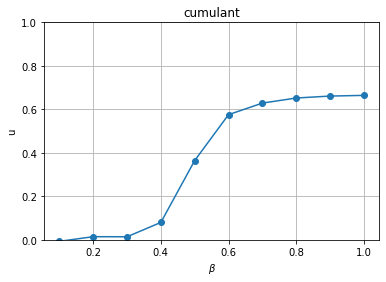
\includegraphics[width=\textwidth]{../images/dense_cumulant.png} 
		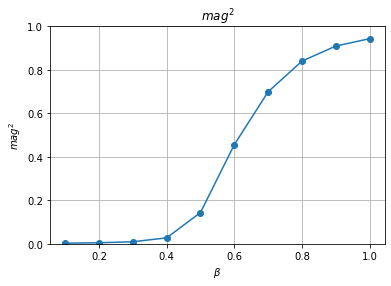
\includegraphics[width=\textwidth]{../images/dense_magnetization.png} 
		\caption{Плотная}
	\end{subfigure}
	\begin{subfigure}[t]{0.48\textwidth}
		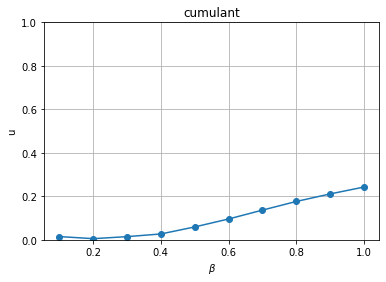
\includegraphics[width=\textwidth]{../images/loose_cumulant.png} 
		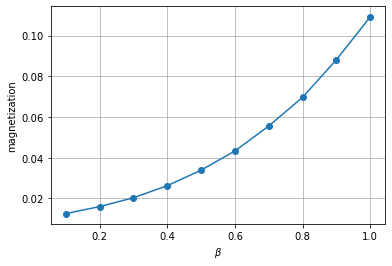
\includegraphics[width=\textwidth]{../images/loose_magnetization.png} 
		\caption{Неплотная}
	\end{subfigure}
	\caption{Пример кумулянта и намагниченности плотной и неплотной конформаций}
\end{figure}


\subsubsection{Разделение конформаций}

Для отделения плотных конформаций от остальных было предложено вычислять их радиус инерции.$R = \sqrt{\frac{1}{n}\sum_{i=1}^{n}r_{i}^{2}}$, где $r_i$ это расстояние от узла конформации до её центра масс. Однако при рассмотрении большого количества конформаций оказалось, что маленький радиус инерции не гарантирует хорошую намагниченность конформации

\begin{figure}[h]
	\centering
	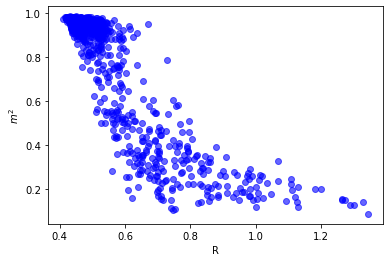
\includegraphics[width=\textwidth]{../images/mag2_to_R_L250.png} 
	\caption{Корреляция намагниченности конформаций при $\beta = 1$ и радиуса инерции для конформаций длины $L = 250$}
	\label{fig:mag2_to_R} 
\end{figure}

На рис.\ref{fig:mag2_to_R}, при $R \approx 0.6$ $m^2$ принимают любые значения от $0.2$ до $1.0$. Значит, при разделении конформации только по радиусу инерции, мы либо будем отбрасывать намагничивающиеся конформации, либо оставлять не намагничивающиеся

\paragraph{Кластеризованные конформации}

\begin{figure}[h!]
	\centering
	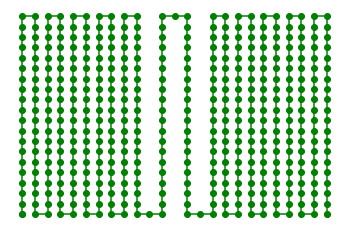
\includegraphics[width=0.47\textwidth]{../images/2Cluster_conformation.png}
	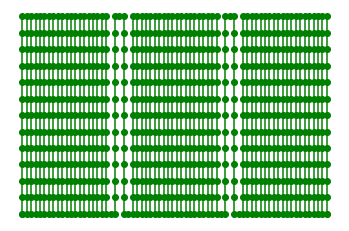
\includegraphics[width=0.47\textwidth]{../images/3Cluster_conformation.png} 
	\caption{Пример плотной немагнитной конформации}
	\label{fig:synth_cluster_conf}
\end{figure}

На искусственном примере рис.\ref{fig:synth_cluster_conf} показана одна из причин, по которой плотная конформация может плохо намагничиваться. Тут имеется несколько крупных двумерных кластеров, соединённых одномерной цепочкой. И не смотря на то, что сами по себе эти кластеры намагничиваются, направление спинов в них слабо связано, из-за чего спины в разных кластерах с большой вероятностью будут направлены в противоположные стороны.


Следующей задачей стало проанализировать конформации на количество и размеры кластеров, а так же мостов(одномерных сегментов) которые и соединяют. Первым вариантом было искать классические мосты -- спины, при удалении увеличивается число компонент связанности. Однако такой способ не дал желаемого эффекта, так как кластеры могут быть соединены более чем одним мостом. И например на конформации из рис. \ref{fig:clusters_and_bridges} данный способ не выделяет ни одного моста. Следующий алгоритм выделял как мосты все цепочки спинов у которых 1 или 2 соседа, однако при таком подходе мы получаем мосты, которые соединяют один и тот же кластер. Такие мосты не разделяют кластеры и незначительно влияют на намагниченность конформации.

Итоговая версия алгоритма выделяет как мосты все спины, которые имеют 1 или 2 соседа, и затем добавляет мосты, которые соединяют один и тот же кластер, к этому же кластеру.

\paragraph{Алгоритм разбиения на мосты и кластеры}
\begin{enumerate}
	\item Отметить все спины с 1 или 2 соседями как мосты.
	\item Создаём массив, где отмечаем посещённые спины. Создаём массив где для каждого спина будем писать номер его кластера. И переменную отвечающую за текущую длину моста $l$. Изначально все спины не посещены, $l = 0$.
	\item Начинаем идти по конформации от первой вершины.
	\begin{enumerate}
	
		\item Если спин отмечен как мост, то увеличиваем $l$ на 1
		\item Если спин не отмечен как мост, и не посещён. Увеличиваем счётчик кластеров на 1 и запускаем DFS(Алгоритм DFS описан ниже). Если $l > 0$ увеличиваем счётчик мостов на 1, длина нового моста $= l$. Обнуляем $l$
		\item Если спин не мост, уже посещён, последний встреченный спин, не являющийся мостом, принадлежит тому же кластеру и текущая длина моста $l > 0$. Значит этот мост соединяет один и тот же кластер. Поэтому добавляем предыдущие $l$ спинов к этому кластеру, обнуляем $l$.
		\item Если спин не мост, посещён, но номер кластера отличается от последнего встреченного кластера. Если $l > 0$ увеличиваем счётчик мостов на 1, длина нового моста $= l$. Обнуляем $l$
	\end{enumerate}
	\item пройдя всю конформацию, если $l > 0$, создаём ещё один мост
\end{enumerate}

\textbf{Алгоритм DFS}
\begin{enumerate}
	\item Заходим в вершину.
	\item Отмечаем вершину как посещённую.
	\item Отмечаем номер её кластера.
	\item Увеличиваем счётчик размера текущего кластера на 1.
	\item Заходим во все соседние не посещённые вершины не мосты.
\end{enumerate}

В данном алгоритме мы пользуемся тем, что мосты обязательно образуются из подряд идущих спинов конформации. Поэтому чтобы определить соединяет ли мост один и тот же кластер, нам достаточно, идя по конформации, запоминать последний встреченный кластер и сравнивать его с новым.

\begin{figure}[h]
	\centering
	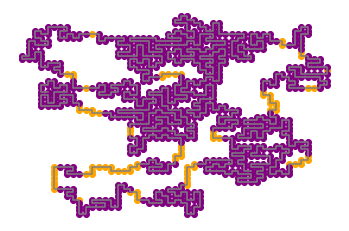
\includegraphics[width=0.70\textwidth]{../images/bridges_example_1.png}  
	\caption{Пример реальных конформаций с маленьким радиусом инерции и маленькой намагниченностью, с отмеченными мостами}
	\label{fig:clusters_and_bridges}
\end{figure}

\subsection{Статистика по кластерам и мостам}
Ниже представлены гистограммы с размерами и числом кластеров и мостов в конформациях. Посчитано на 10000 конформациях с длинами 250, 500, 10000. Размеры кластеров и длины мостов нормированы на длины конформаций. 


\begin{figure}[H]
	\centering
	\begin{subfigure}[t]{0.3\textwidth} 
		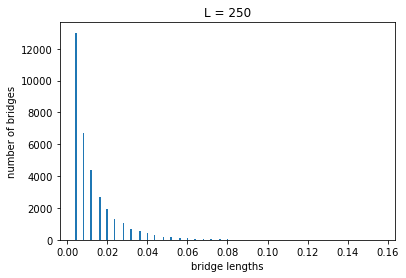
\includegraphics[width=\textwidth]{../images/bridge_lengths_L250.png} 
	\end{subfigure}
	\begin{subfigure}[t]{0.3\textwidth} 
		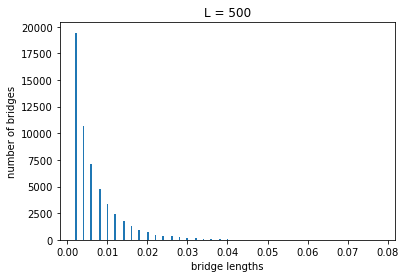
\includegraphics[width=\textwidth]{../images/bridge_lengths_L500.png} 
	\end{subfigure}
	\begin{subfigure}[t]{0.3\textwidth} 
		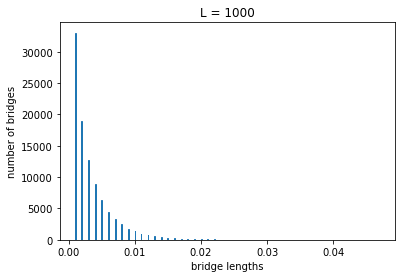
\includegraphics[width=\textwidth]{../images/bridge_lengths_L1000.png} 
	\end{subfigure}
	\caption{Распределение длин мостов.}
\end{figure}

\begin{figure}[H]
	\centering
	\begin{subfigure}[t]{0.3\textwidth} 
		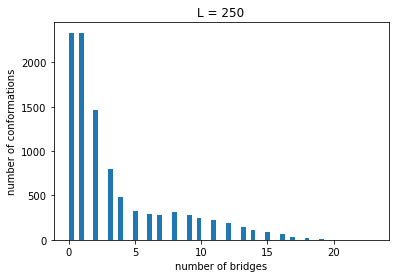
\includegraphics[width=\textwidth]{../images/bridges_count_L250.png} 
	\end{subfigure}
	\begin{subfigure}[t]{0.3\textwidth} 
		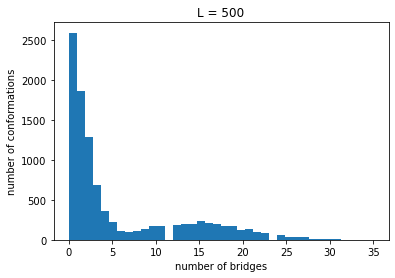
\includegraphics[width=\textwidth]{../images/bridges_count_L500.png} 
	\end{subfigure}
	\begin{subfigure}[t]{0.3\textwidth} 
		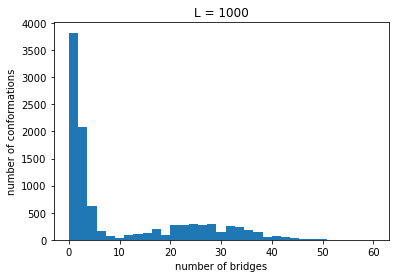
\includegraphics[width=\textwidth]{../images/bridges_count_L1000.png} 
	\end{subfigure}
	\caption{Распределение числа мостов в конформации.}
\end{figure}

\begin{figure}[H]
	\centering
	\begin{subfigure}[t]{0.3\textwidth} 
		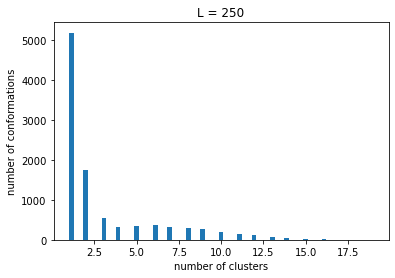
\includegraphics[width=\textwidth]{../images/clusters_count_L250.png} 
	\end{subfigure}
	\begin{subfigure}[t]{0.3\textwidth} 
		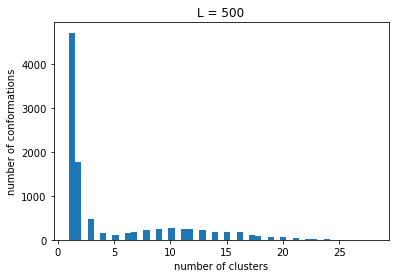
\includegraphics[width=\textwidth]{../images/clusters_count_L500.png} 
	\end{subfigure}
	\begin{subfigure}[t]{0.3\textwidth} 
		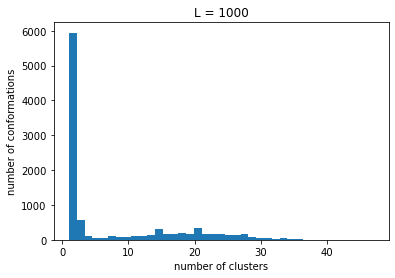
\includegraphics[width=\textwidth]{../images/clusters_count_L1000.png} 
	\end{subfigure}
	\caption{Распределение числа кластеров в конформации.}
\end{figure}

\begin{figure}[H]
	\centering
	\begin{subfigure}[t]{0.3\textwidth} 
		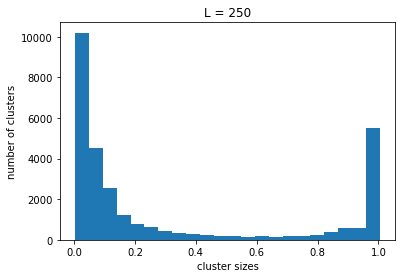
\includegraphics[width=\textwidth]{../images/cluster_sizes_L250.png} 
	\end{subfigure}
	\begin{subfigure}[t]{0.3\textwidth} 
		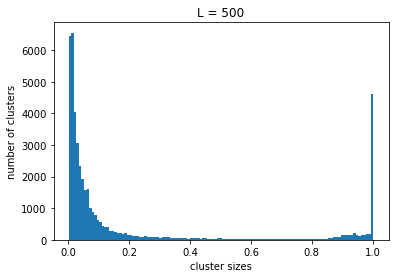
\includegraphics[width=\textwidth]{../images/cluster_sizes_L500.png} 
	\end{subfigure}
	\begin{subfigure}[t]{0.3\textwidth} 
		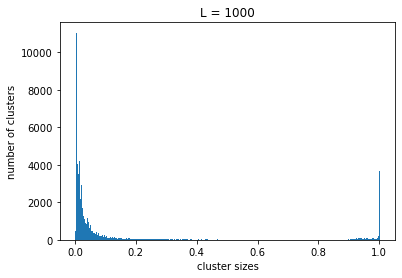
\includegraphics[width=\textwidth]{../images/cluster_sizes_L1000.png} 
	\end{subfigure}
	\caption{Распределение размера кластеров.}
\end{figure}

\begin{figure}[H]
	\centering
	\begin{subfigure}[t]{0.3\textwidth} 
		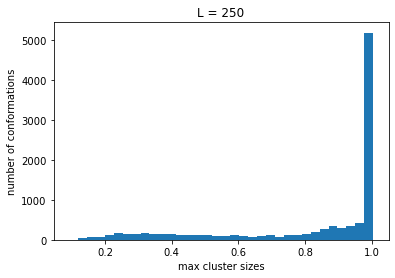
\includegraphics[width=\textwidth]{../images/max_cluster_size_L250.png} 
	\end{subfigure}
	\begin{subfigure}[t]{0.3\textwidth} 
		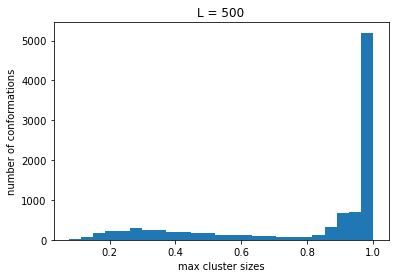
\includegraphics[width=\textwidth]{../images/max_cluster_size_L500.png} 
	\end{subfigure}
	\begin{subfigure}[t]{0.3\textwidth} 
		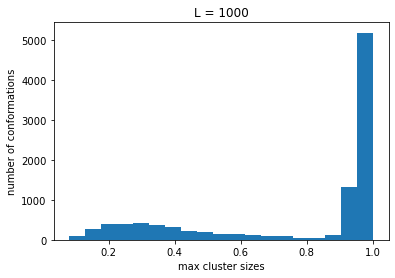
\includegraphics[width=\textwidth]{../images/max_cluster_size_L1000.png} 
	\end{subfigure}
	\caption{Распределение размера наибольшего кластера в конформации.}
\end{figure}


\subsection{Результаты разбиения на кластеры}
Результаты анализа связи между намагниченностью и количеством и размерами кластеров и мостов подтверждают сказанное выше. У конформаций с большим числом кластеров обычно намагниченность ниже чем у конформаций с одним большим кластером. 

Я рассмотрел несколько параметров: количество мостов, количество кластеров, суммарная длина мостов, размер наибольшего кластера. Наилучшим способом разделения конформаций на магнитные и немагнитные сейчас выглядит именно разделение по размеру наибольшего кластера. Как видно на рис \ref{fig:mag_from_max_cluster} при разбиении по данному параметру разброс намагниченности значительно ниже, чем при разбиении по радиусу инерции. Данный параметр можно легко масштабировать для разных длин конформаций.

\begin{figure}[h]
	\centering
	\caption{График размера наибольшего кластера и квадрата намагниченности для 10000 конформаций длины 1000}
	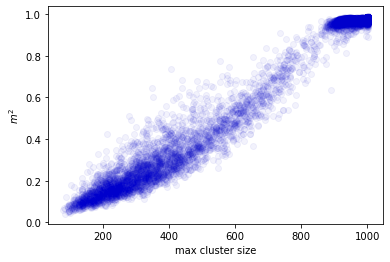
\includegraphics[width=0.8\textwidth]{../images/mag_from_cluster_size.png} 
	\label{fig:mag_from_max_cluster}
\end{figure}

\paragraph{Сравнение разделения по кластерам и по радиусу}
Чтобы оценить и сравнить эффективность разбиения конформаций при помощи размера наибольшего кластера и радиуса инерции воспользуемся следующим способом.

\begin{enumerate}
	\item Зададим значение намагниченности $\mu$, начиная с которого будем считать конформации намагниченными.
	\item Из всех сгенерированных конформаций возьмём $n$ конформаций с наименьшими радисоми инерции, и $n$ конформаций с наибольшими размерами кластеров.
	\item Среди выбранных конформаций посчитаем $k_{\mu, n}$ количество конформаций, намагниченность которых $< \mu$. Чем ниже это значение, тем лучше соответствующий способ разделения.
	\item Повторяем предыдущие пункты для разных значений $\mu$ и $n$.
\end{enumerate}

Сравнивая полученные значения $k_{\mu, n}$ можем определить, какой из способов эффективнее. На рис.\ref{fig:kmun_example} видно как примерно ведут себя данные значения: до определённого n они равны 0, затем, дойдя до границы между магнитными и немагнитными конформациями, оно начинает расти, после чего рост становится линейным, так как все оставшиеся конформации не являются магнитными. 
Лучше разницу между двумя способами видно на рис.\ref{fig:kmun_dif}, где при всех значениях $\mu$ и $n$ $k_{\mu, n}$ остаётся отрицательным. То есть разделения по радиусу инерции всегда оставляет больше немагнитных конформаций, чем разделение по размеру кластеров.

\begin{figure}[h]
	\centering
	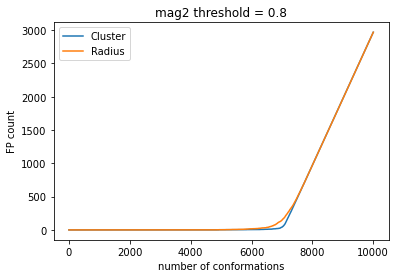
\includegraphics[width=0.6\textwidth]{../images/cluster_and_radius_mu0.8.png} 
	\caption{График $k_{\mu, n}$ для разделения по кластерам и по радиусу, при $\mu = 0.8$.}
	\label{fig:kmun_example}
\end{figure}

\begin{figure}[h]
	\centering
	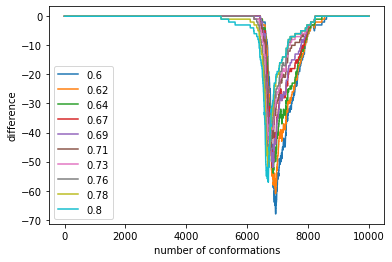
\includegraphics[width=0.8\textwidth]{../images/radius_and_cluster_comparising_L1000.png}
	\label{fig:kmun_dif}
	\caption{График разности: $k_{\mu, n}$ при кластерном разделении - $k_{\mu, n}$ при разделении по радиусам. На 10000 конформаций длины 1000. Каждая линия соответствует одному значению $\mu$.}
\end{figure}





\subsection{Кумулянт и точка перехода}

Кумулянт Биндера для одной реплики при заданной температуре вычисляется по формуле $U = 1 - \frac{\langle m^4\rangle}{3\langle m^2\rangle ^2}$. Дальше Значения усредняются между репликами при каждой температуре $\langle U\rangle = \frac{1}{n}\sum_{i=1}^{n}U_i$ 
Погрешность кумулянта от реплики к реплике вычисляется как среднеквадратичное отклонение по формуле $\sqrt{\frac{1}{n}\sum_{i=1}^{n}(\langle U\rangle - U_i)^2}$


Эксперименты с разделением конформаций по радиусу инерции показали, что таким образом можно выделить наборы конформаций разных длин так, что для них будет возможно найти точку перехода.

\begin{figure}[h]
	\centering
	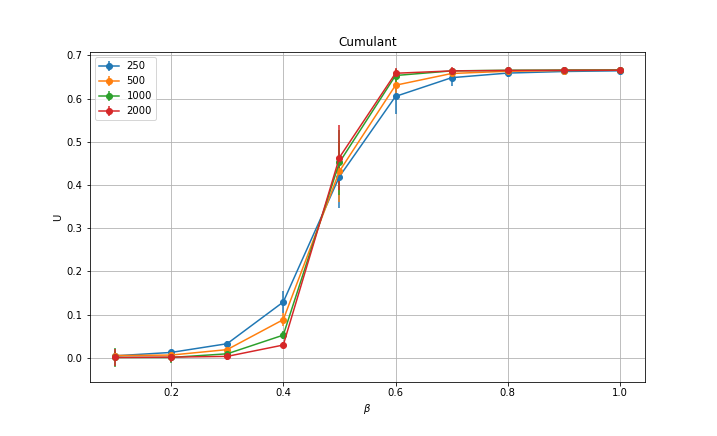
\includegraphics[width=1\textwidth]{../images/Cumulant_big.png} 
	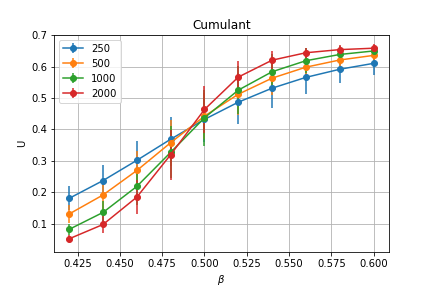
\includegraphics[width=1\textwidth]{../images/Cumulant_beta0.4_0.6.png} 
	\caption{Значения куулянтов после отбрасывания конформаций по радиусам}
\end{figure}


\section{Магнитная восприимчивость}
Один из способов определить точку перехода это определить пик магнитной восприимчивости конформаций. Как описано в \cite{swendsen} точка магнитного перехода и пик магнитной восприимчивости должны совпадать. Если пик отсутствует, значит отсутствует точка магнитного перехода.

Магнитная восприимчивость это отношение намагниченности конформации к напряжённость внешнего поля. Ожидается, что в намагничивающихся конформациях в точке перехода должен наблюдаться пик магнитной восприимчивости, в то время как в не намагничивающихся магнитная восприимчивость не будет иметь пиков.

Получим формулу для магнитной восприимчивости конформации.

По определению
\[
	\chi = \frac{\partial\langle |M|\rangle}{\partial h}
\]
Подставим формулу намагниченности и продифференцируем.
\[
	\frac{\sum_\sigma {|M| e^{-\beta H} \left( -\beta \frac{\partial H}{\partial h}\right)} \cdot Z - \sum_\sigma {|M| e^{-\beta H}} \cdot \sum_\sigma {e^{-\beta H} \left( -\beta \frac{\partial H}{\partial h}\right)}}{Z^2}
\]

Заметим, что

\[
	\frac{\partial H}{\partial h} = -\sum_i\sigma_i = -|M|
\]
Тогда
\[
	\chi = \frac{\partial\langle |M|\rangle}{\partial h} = \frac{\sum_\sigma {Z\beta M^2 e^{-\beta H}} - \sum_\sigma {|M| e^{-\beta H}}\cdot \sum_\sigma {\beta |M| e^{-\beta H}}}{Z^2} = \beta \left(\langle M^2\rangle - \langle |M| \rangle^2 \right)
\]


По данной формуле мы можем вычислить магнитную восприимчивость конформаций, используя значения абсолютной намагниченности и квадрата намагниченности, полученные при при расчёте модели Изинга.



\subsection{Результаты замеров}
Для рассмотрения были взяты 10000 конформаций с длинами 250, 500 и 1000. Замеры были сделаны при 10 значениях $\beta$, линейно распределённых от 0.1 до 1.0.

Все конформации либо имеют единственный пик магнитной восприимчивости, либо магнитная восприимчивость непрерывно возрастает с увеличением $\beta$.

\begin{figure}[htb]
	\centering
	%% Creator: Matplotlib, PGF backend
%%
%% To include the figure in your LaTeX document, write
%%   \input{<filename>.pgf}
%%
%% Make sure the required packages are loaded in your preamble
%%   \usepackage{pgf}
%%
%% Also ensure that all the required font packages are loaded; for instance,
%% the lmodern package is sometimes necessary when using math font.
%%   \usepackage{lmodern}
%%
%% Figures using additional raster images can only be included by \input if
%% they are in the same directory as the main LaTeX file. For loading figures
%% from other directories you can use the `import` package
%%   \usepackage{import}
%%
%% and then include the figures with
%%   \import{<path to file>}{<filename>.pgf}
%%
%% Matplotlib used the following preamble
%%   
%%   \makeatletter\@ifpackageloaded{underscore}{}{\usepackage[strings]{underscore}}\makeatother
%%
\begingroup%
\makeatletter%
\begin{pgfpicture}%
\pgfpathrectangle{\pgfpointorigin}{\pgfqpoint{4.453681in}{2.871460in}}%
\pgfusepath{use as bounding box, clip}%
\begin{pgfscope}%
\pgfsetbuttcap%
\pgfsetmiterjoin%
\definecolor{currentfill}{rgb}{1.000000,1.000000,1.000000}%
\pgfsetfillcolor{currentfill}%
\pgfsetlinewidth{0.000000pt}%
\definecolor{currentstroke}{rgb}{1.000000,1.000000,1.000000}%
\pgfsetstrokecolor{currentstroke}%
\pgfsetdash{}{0pt}%
\pgfpathmoveto{\pgfqpoint{0.000000in}{0.000000in}}%
\pgfpathlineto{\pgfqpoint{4.453681in}{0.000000in}}%
\pgfpathlineto{\pgfqpoint{4.453681in}{2.871460in}}%
\pgfpathlineto{\pgfqpoint{0.000000in}{2.871460in}}%
\pgfpathlineto{\pgfqpoint{0.000000in}{0.000000in}}%
\pgfpathclose%
\pgfusepath{fill}%
\end{pgfscope}%
\begin{pgfscope}%
\pgfsetbuttcap%
\pgfsetmiterjoin%
\definecolor{currentfill}{rgb}{1.000000,1.000000,1.000000}%
\pgfsetfillcolor{currentfill}%
\pgfsetlinewidth{0.000000pt}%
\definecolor{currentstroke}{rgb}{0.000000,0.000000,0.000000}%
\pgfsetstrokecolor{currentstroke}%
\pgfsetstrokeopacity{0.000000}%
\pgfsetdash{}{0pt}%
\pgfpathmoveto{\pgfqpoint{0.654013in}{0.499691in}}%
\pgfpathlineto{\pgfqpoint{4.353681in}{0.499691in}}%
\pgfpathlineto{\pgfqpoint{4.353681in}{2.771460in}}%
\pgfpathlineto{\pgfqpoint{0.654013in}{2.771460in}}%
\pgfpathlineto{\pgfqpoint{0.654013in}{0.499691in}}%
\pgfpathclose%
\pgfusepath{fill}%
\end{pgfscope}%
\begin{pgfscope}%
\pgfpathrectangle{\pgfqpoint{0.654013in}{0.499691in}}{\pgfqpoint{3.699668in}{2.271769in}}%
\pgfusepath{clip}%
\pgfsetbuttcap%
\pgfsetmiterjoin%
\definecolor{currentfill}{rgb}{0.121569,0.466667,0.705882}%
\pgfsetfillcolor{currentfill}%
\pgfsetlinewidth{0.000000pt}%
\definecolor{currentstroke}{rgb}{0.000000,0.000000,0.000000}%
\pgfsetstrokecolor{currentstroke}%
\pgfsetstrokeopacity{0.000000}%
\pgfsetdash{}{0pt}%
\pgfpathmoveto{\pgfqpoint{0.822180in}{0.499691in}}%
\pgfpathlineto{\pgfqpoint{0.859970in}{0.499691in}}%
\pgfpathlineto{\pgfqpoint{0.859970in}{1.830176in}}%
\pgfpathlineto{\pgfqpoint{0.822180in}{1.830176in}}%
\pgfpathlineto{\pgfqpoint{0.822180in}{0.499691in}}%
\pgfpathclose%
\pgfusepath{fill}%
\end{pgfscope}%
\begin{pgfscope}%
\pgfpathrectangle{\pgfqpoint{0.654013in}{0.499691in}}{\pgfqpoint{3.699668in}{2.271769in}}%
\pgfusepath{clip}%
\pgfsetbuttcap%
\pgfsetmiterjoin%
\definecolor{currentfill}{rgb}{0.121569,0.466667,0.705882}%
\pgfsetfillcolor{currentfill}%
\pgfsetlinewidth{0.000000pt}%
\definecolor{currentstroke}{rgb}{0.000000,0.000000,0.000000}%
\pgfsetstrokecolor{currentstroke}%
\pgfsetstrokeopacity{0.000000}%
\pgfsetdash{}{0pt}%
\pgfpathmoveto{\pgfqpoint{1.011131in}{0.499691in}}%
\pgfpathlineto{\pgfqpoint{1.048921in}{0.499691in}}%
\pgfpathlineto{\pgfqpoint{1.048921in}{0.499691in}}%
\pgfpathlineto{\pgfqpoint{1.011131in}{0.499691in}}%
\pgfpathlineto{\pgfqpoint{1.011131in}{0.499691in}}%
\pgfpathclose%
\pgfusepath{fill}%
\end{pgfscope}%
\begin{pgfscope}%
\pgfpathrectangle{\pgfqpoint{0.654013in}{0.499691in}}{\pgfqpoint{3.699668in}{2.271769in}}%
\pgfusepath{clip}%
\pgfsetbuttcap%
\pgfsetmiterjoin%
\definecolor{currentfill}{rgb}{0.121569,0.466667,0.705882}%
\pgfsetfillcolor{currentfill}%
\pgfsetlinewidth{0.000000pt}%
\definecolor{currentstroke}{rgb}{0.000000,0.000000,0.000000}%
\pgfsetstrokecolor{currentstroke}%
\pgfsetstrokeopacity{0.000000}%
\pgfsetdash{}{0pt}%
\pgfpathmoveto{\pgfqpoint{1.200083in}{0.499691in}}%
\pgfpathlineto{\pgfqpoint{1.237873in}{0.499691in}}%
\pgfpathlineto{\pgfqpoint{1.237873in}{0.499691in}}%
\pgfpathlineto{\pgfqpoint{1.200083in}{0.499691in}}%
\pgfpathlineto{\pgfqpoint{1.200083in}{0.499691in}}%
\pgfpathclose%
\pgfusepath{fill}%
\end{pgfscope}%
\begin{pgfscope}%
\pgfpathrectangle{\pgfqpoint{0.654013in}{0.499691in}}{\pgfqpoint{3.699668in}{2.271769in}}%
\pgfusepath{clip}%
\pgfsetbuttcap%
\pgfsetmiterjoin%
\definecolor{currentfill}{rgb}{0.121569,0.466667,0.705882}%
\pgfsetfillcolor{currentfill}%
\pgfsetlinewidth{0.000000pt}%
\definecolor{currentstroke}{rgb}{0.000000,0.000000,0.000000}%
\pgfsetstrokecolor{currentstroke}%
\pgfsetstrokeopacity{0.000000}%
\pgfsetdash{}{0pt}%
\pgfpathmoveto{\pgfqpoint{1.389034in}{0.499691in}}%
\pgfpathlineto{\pgfqpoint{1.426824in}{0.499691in}}%
\pgfpathlineto{\pgfqpoint{1.426824in}{1.538228in}}%
\pgfpathlineto{\pgfqpoint{1.389034in}{1.538228in}}%
\pgfpathlineto{\pgfqpoint{1.389034in}{0.499691in}}%
\pgfpathclose%
\pgfusepath{fill}%
\end{pgfscope}%
\begin{pgfscope}%
\pgfpathrectangle{\pgfqpoint{0.654013in}{0.499691in}}{\pgfqpoint{3.699668in}{2.271769in}}%
\pgfusepath{clip}%
\pgfsetbuttcap%
\pgfsetmiterjoin%
\definecolor{currentfill}{rgb}{0.121569,0.466667,0.705882}%
\pgfsetfillcolor{currentfill}%
\pgfsetlinewidth{0.000000pt}%
\definecolor{currentstroke}{rgb}{0.000000,0.000000,0.000000}%
\pgfsetstrokecolor{currentstroke}%
\pgfsetstrokeopacity{0.000000}%
\pgfsetdash{}{0pt}%
\pgfpathmoveto{\pgfqpoint{1.577985in}{0.499691in}}%
\pgfpathlineto{\pgfqpoint{1.615776in}{0.499691in}}%
\pgfpathlineto{\pgfqpoint{1.615776in}{0.499691in}}%
\pgfpathlineto{\pgfqpoint{1.577985in}{0.499691in}}%
\pgfpathlineto{\pgfqpoint{1.577985in}{0.499691in}}%
\pgfpathclose%
\pgfusepath{fill}%
\end{pgfscope}%
\begin{pgfscope}%
\pgfpathrectangle{\pgfqpoint{0.654013in}{0.499691in}}{\pgfqpoint{3.699668in}{2.271769in}}%
\pgfusepath{clip}%
\pgfsetbuttcap%
\pgfsetmiterjoin%
\definecolor{currentfill}{rgb}{0.121569,0.466667,0.705882}%
\pgfsetfillcolor{currentfill}%
\pgfsetlinewidth{0.000000pt}%
\definecolor{currentstroke}{rgb}{0.000000,0.000000,0.000000}%
\pgfsetstrokecolor{currentstroke}%
\pgfsetstrokeopacity{0.000000}%
\pgfsetdash{}{0pt}%
\pgfpathmoveto{\pgfqpoint{1.766937in}{0.499691in}}%
\pgfpathlineto{\pgfqpoint{1.804727in}{0.499691in}}%
\pgfpathlineto{\pgfqpoint{1.804727in}{0.499691in}}%
\pgfpathlineto{\pgfqpoint{1.766937in}{0.499691in}}%
\pgfpathlineto{\pgfqpoint{1.766937in}{0.499691in}}%
\pgfpathclose%
\pgfusepath{fill}%
\end{pgfscope}%
\begin{pgfscope}%
\pgfpathrectangle{\pgfqpoint{0.654013in}{0.499691in}}{\pgfqpoint{3.699668in}{2.271769in}}%
\pgfusepath{clip}%
\pgfsetbuttcap%
\pgfsetmiterjoin%
\definecolor{currentfill}{rgb}{0.121569,0.466667,0.705882}%
\pgfsetfillcolor{currentfill}%
\pgfsetlinewidth{0.000000pt}%
\definecolor{currentstroke}{rgb}{0.000000,0.000000,0.000000}%
\pgfsetstrokecolor{currentstroke}%
\pgfsetstrokeopacity{0.000000}%
\pgfsetdash{}{0pt}%
\pgfpathmoveto{\pgfqpoint{1.955888in}{0.499691in}}%
\pgfpathlineto{\pgfqpoint{1.993678in}{0.499691in}}%
\pgfpathlineto{\pgfqpoint{1.993678in}{0.499691in}}%
\pgfpathlineto{\pgfqpoint{1.955888in}{0.499691in}}%
\pgfpathlineto{\pgfqpoint{1.955888in}{0.499691in}}%
\pgfpathclose%
\pgfusepath{fill}%
\end{pgfscope}%
\begin{pgfscope}%
\pgfpathrectangle{\pgfqpoint{0.654013in}{0.499691in}}{\pgfqpoint{3.699668in}{2.271769in}}%
\pgfusepath{clip}%
\pgfsetbuttcap%
\pgfsetmiterjoin%
\definecolor{currentfill}{rgb}{0.121569,0.466667,0.705882}%
\pgfsetfillcolor{currentfill}%
\pgfsetlinewidth{0.000000pt}%
\definecolor{currentstroke}{rgb}{0.000000,0.000000,0.000000}%
\pgfsetstrokecolor{currentstroke}%
\pgfsetstrokeopacity{0.000000}%
\pgfsetdash{}{0pt}%
\pgfpathmoveto{\pgfqpoint{2.144839in}{0.499691in}}%
\pgfpathlineto{\pgfqpoint{2.182630in}{0.499691in}}%
\pgfpathlineto{\pgfqpoint{2.182630in}{0.662038in}}%
\pgfpathlineto{\pgfqpoint{2.144839in}{0.662038in}}%
\pgfpathlineto{\pgfqpoint{2.144839in}{0.499691in}}%
\pgfpathclose%
\pgfusepath{fill}%
\end{pgfscope}%
\begin{pgfscope}%
\pgfpathrectangle{\pgfqpoint{0.654013in}{0.499691in}}{\pgfqpoint{3.699668in}{2.271769in}}%
\pgfusepath{clip}%
\pgfsetbuttcap%
\pgfsetmiterjoin%
\definecolor{currentfill}{rgb}{0.121569,0.466667,0.705882}%
\pgfsetfillcolor{currentfill}%
\pgfsetlinewidth{0.000000pt}%
\definecolor{currentstroke}{rgb}{0.000000,0.000000,0.000000}%
\pgfsetstrokecolor{currentstroke}%
\pgfsetstrokeopacity{0.000000}%
\pgfsetdash{}{0pt}%
\pgfpathmoveto{\pgfqpoint{2.333791in}{0.499691in}}%
\pgfpathlineto{\pgfqpoint{2.371581in}{0.499691in}}%
\pgfpathlineto{\pgfqpoint{2.371581in}{0.499691in}}%
\pgfpathlineto{\pgfqpoint{2.333791in}{0.499691in}}%
\pgfpathlineto{\pgfqpoint{2.333791in}{0.499691in}}%
\pgfpathclose%
\pgfusepath{fill}%
\end{pgfscope}%
\begin{pgfscope}%
\pgfpathrectangle{\pgfqpoint{0.654013in}{0.499691in}}{\pgfqpoint{3.699668in}{2.271769in}}%
\pgfusepath{clip}%
\pgfsetbuttcap%
\pgfsetmiterjoin%
\definecolor{currentfill}{rgb}{0.121569,0.466667,0.705882}%
\pgfsetfillcolor{currentfill}%
\pgfsetlinewidth{0.000000pt}%
\definecolor{currentstroke}{rgb}{0.000000,0.000000,0.000000}%
\pgfsetstrokecolor{currentstroke}%
\pgfsetstrokeopacity{0.000000}%
\pgfsetdash{}{0pt}%
\pgfpathmoveto{\pgfqpoint{2.522742in}{0.499691in}}%
\pgfpathlineto{\pgfqpoint{2.560532in}{0.499691in}}%
\pgfpathlineto{\pgfqpoint{2.560532in}{0.499691in}}%
\pgfpathlineto{\pgfqpoint{2.522742in}{0.499691in}}%
\pgfpathlineto{\pgfqpoint{2.522742in}{0.499691in}}%
\pgfpathclose%
\pgfusepath{fill}%
\end{pgfscope}%
\begin{pgfscope}%
\pgfpathrectangle{\pgfqpoint{0.654013in}{0.499691in}}{\pgfqpoint{3.699668in}{2.271769in}}%
\pgfusepath{clip}%
\pgfsetbuttcap%
\pgfsetmiterjoin%
\definecolor{currentfill}{rgb}{0.121569,0.466667,0.705882}%
\pgfsetfillcolor{currentfill}%
\pgfsetlinewidth{0.000000pt}%
\definecolor{currentstroke}{rgb}{0.000000,0.000000,0.000000}%
\pgfsetstrokecolor{currentstroke}%
\pgfsetstrokeopacity{0.000000}%
\pgfsetdash{}{0pt}%
\pgfpathmoveto{\pgfqpoint{2.711694in}{0.499691in}}%
\pgfpathlineto{\pgfqpoint{2.749484in}{0.499691in}}%
\pgfpathlineto{\pgfqpoint{2.749484in}{0.560700in}}%
\pgfpathlineto{\pgfqpoint{2.711694in}{0.560700in}}%
\pgfpathlineto{\pgfqpoint{2.711694in}{0.499691in}}%
\pgfpathclose%
\pgfusepath{fill}%
\end{pgfscope}%
\begin{pgfscope}%
\pgfpathrectangle{\pgfqpoint{0.654013in}{0.499691in}}{\pgfqpoint{3.699668in}{2.271769in}}%
\pgfusepath{clip}%
\pgfsetbuttcap%
\pgfsetmiterjoin%
\definecolor{currentfill}{rgb}{0.121569,0.466667,0.705882}%
\pgfsetfillcolor{currentfill}%
\pgfsetlinewidth{0.000000pt}%
\definecolor{currentstroke}{rgb}{0.000000,0.000000,0.000000}%
\pgfsetstrokecolor{currentstroke}%
\pgfsetstrokeopacity{0.000000}%
\pgfsetdash{}{0pt}%
\pgfpathmoveto{\pgfqpoint{2.900645in}{0.499691in}}%
\pgfpathlineto{\pgfqpoint{2.938435in}{0.499691in}}%
\pgfpathlineto{\pgfqpoint{2.938435in}{0.499691in}}%
\pgfpathlineto{\pgfqpoint{2.900645in}{0.499691in}}%
\pgfpathlineto{\pgfqpoint{2.900645in}{0.499691in}}%
\pgfpathclose%
\pgfusepath{fill}%
\end{pgfscope}%
\begin{pgfscope}%
\pgfpathrectangle{\pgfqpoint{0.654013in}{0.499691in}}{\pgfqpoint{3.699668in}{2.271769in}}%
\pgfusepath{clip}%
\pgfsetbuttcap%
\pgfsetmiterjoin%
\definecolor{currentfill}{rgb}{0.121569,0.466667,0.705882}%
\pgfsetfillcolor{currentfill}%
\pgfsetlinewidth{0.000000pt}%
\definecolor{currentstroke}{rgb}{0.000000,0.000000,0.000000}%
\pgfsetstrokecolor{currentstroke}%
\pgfsetstrokeopacity{0.000000}%
\pgfsetdash{}{0pt}%
\pgfpathmoveto{\pgfqpoint{3.089596in}{0.499691in}}%
\pgfpathlineto{\pgfqpoint{3.127387in}{0.499691in}}%
\pgfpathlineto{\pgfqpoint{3.127387in}{0.499691in}}%
\pgfpathlineto{\pgfqpoint{3.089596in}{0.499691in}}%
\pgfpathlineto{\pgfqpoint{3.089596in}{0.499691in}}%
\pgfpathclose%
\pgfusepath{fill}%
\end{pgfscope}%
\begin{pgfscope}%
\pgfpathrectangle{\pgfqpoint{0.654013in}{0.499691in}}{\pgfqpoint{3.699668in}{2.271769in}}%
\pgfusepath{clip}%
\pgfsetbuttcap%
\pgfsetmiterjoin%
\definecolor{currentfill}{rgb}{0.121569,0.466667,0.705882}%
\pgfsetfillcolor{currentfill}%
\pgfsetlinewidth{0.000000pt}%
\definecolor{currentstroke}{rgb}{0.000000,0.000000,0.000000}%
\pgfsetstrokecolor{currentstroke}%
\pgfsetstrokeopacity{0.000000}%
\pgfsetdash{}{0pt}%
\pgfpathmoveto{\pgfqpoint{3.278548in}{0.499691in}}%
\pgfpathlineto{\pgfqpoint{3.316338in}{0.499691in}}%
\pgfpathlineto{\pgfqpoint{3.316338in}{0.499691in}}%
\pgfpathlineto{\pgfqpoint{3.278548in}{0.499691in}}%
\pgfpathlineto{\pgfqpoint{3.278548in}{0.499691in}}%
\pgfpathclose%
\pgfusepath{fill}%
\end{pgfscope}%
\begin{pgfscope}%
\pgfpathrectangle{\pgfqpoint{0.654013in}{0.499691in}}{\pgfqpoint{3.699668in}{2.271769in}}%
\pgfusepath{clip}%
\pgfsetbuttcap%
\pgfsetmiterjoin%
\definecolor{currentfill}{rgb}{0.121569,0.466667,0.705882}%
\pgfsetfillcolor{currentfill}%
\pgfsetlinewidth{0.000000pt}%
\definecolor{currentstroke}{rgb}{0.000000,0.000000,0.000000}%
\pgfsetstrokecolor{currentstroke}%
\pgfsetstrokeopacity{0.000000}%
\pgfsetdash{}{0pt}%
\pgfpathmoveto{\pgfqpoint{3.467499in}{0.499691in}}%
\pgfpathlineto{\pgfqpoint{3.505289in}{0.499691in}}%
\pgfpathlineto{\pgfqpoint{3.505289in}{0.546568in}}%
\pgfpathlineto{\pgfqpoint{3.467499in}{0.546568in}}%
\pgfpathlineto{\pgfqpoint{3.467499in}{0.499691in}}%
\pgfpathclose%
\pgfusepath{fill}%
\end{pgfscope}%
\begin{pgfscope}%
\pgfpathrectangle{\pgfqpoint{0.654013in}{0.499691in}}{\pgfqpoint{3.699668in}{2.271769in}}%
\pgfusepath{clip}%
\pgfsetbuttcap%
\pgfsetmiterjoin%
\definecolor{currentfill}{rgb}{0.121569,0.466667,0.705882}%
\pgfsetfillcolor{currentfill}%
\pgfsetlinewidth{0.000000pt}%
\definecolor{currentstroke}{rgb}{0.000000,0.000000,0.000000}%
\pgfsetstrokecolor{currentstroke}%
\pgfsetstrokeopacity{0.000000}%
\pgfsetdash{}{0pt}%
\pgfpathmoveto{\pgfqpoint{3.656450in}{0.499691in}}%
\pgfpathlineto{\pgfqpoint{3.694241in}{0.499691in}}%
\pgfpathlineto{\pgfqpoint{3.694241in}{0.499691in}}%
\pgfpathlineto{\pgfqpoint{3.656450in}{0.499691in}}%
\pgfpathlineto{\pgfqpoint{3.656450in}{0.499691in}}%
\pgfpathclose%
\pgfusepath{fill}%
\end{pgfscope}%
\begin{pgfscope}%
\pgfpathrectangle{\pgfqpoint{0.654013in}{0.499691in}}{\pgfqpoint{3.699668in}{2.271769in}}%
\pgfusepath{clip}%
\pgfsetbuttcap%
\pgfsetmiterjoin%
\definecolor{currentfill}{rgb}{0.121569,0.466667,0.705882}%
\pgfsetfillcolor{currentfill}%
\pgfsetlinewidth{0.000000pt}%
\definecolor{currentstroke}{rgb}{0.000000,0.000000,0.000000}%
\pgfsetstrokecolor{currentstroke}%
\pgfsetstrokeopacity{0.000000}%
\pgfsetdash{}{0pt}%
\pgfpathmoveto{\pgfqpoint{3.845402in}{0.499691in}}%
\pgfpathlineto{\pgfqpoint{3.883192in}{0.499691in}}%
\pgfpathlineto{\pgfqpoint{3.883192in}{0.499691in}}%
\pgfpathlineto{\pgfqpoint{3.845402in}{0.499691in}}%
\pgfpathlineto{\pgfqpoint{3.845402in}{0.499691in}}%
\pgfpathclose%
\pgfusepath{fill}%
\end{pgfscope}%
\begin{pgfscope}%
\pgfpathrectangle{\pgfqpoint{0.654013in}{0.499691in}}{\pgfqpoint{3.699668in}{2.271769in}}%
\pgfusepath{clip}%
\pgfsetbuttcap%
\pgfsetmiterjoin%
\definecolor{currentfill}{rgb}{0.121569,0.466667,0.705882}%
\pgfsetfillcolor{currentfill}%
\pgfsetlinewidth{0.000000pt}%
\definecolor{currentstroke}{rgb}{0.000000,0.000000,0.000000}%
\pgfsetstrokecolor{currentstroke}%
\pgfsetstrokeopacity{0.000000}%
\pgfsetdash{}{0pt}%
\pgfpathmoveto{\pgfqpoint{4.034353in}{0.499691in}}%
\pgfpathlineto{\pgfqpoint{4.072143in}{0.499691in}}%
\pgfpathlineto{\pgfqpoint{4.072143in}{1.307289in}}%
\pgfpathlineto{\pgfqpoint{4.034353in}{1.307289in}}%
\pgfpathlineto{\pgfqpoint{4.034353in}{0.499691in}}%
\pgfpathclose%
\pgfusepath{fill}%
\end{pgfscope}%
\begin{pgfscope}%
\pgfpathrectangle{\pgfqpoint{0.654013in}{0.499691in}}{\pgfqpoint{3.699668in}{2.271769in}}%
\pgfusepath{clip}%
\pgfsetbuttcap%
\pgfsetmiterjoin%
\definecolor{currentfill}{rgb}{1.000000,0.498039,0.054902}%
\pgfsetfillcolor{currentfill}%
\pgfsetlinewidth{0.000000pt}%
\definecolor{currentstroke}{rgb}{0.000000,0.000000,0.000000}%
\pgfsetstrokecolor{currentstroke}%
\pgfsetstrokeopacity{0.000000}%
\pgfsetdash{}{0pt}%
\pgfpathmoveto{\pgfqpoint{0.859970in}{0.499691in}}%
\pgfpathlineto{\pgfqpoint{0.897760in}{0.499691in}}%
\pgfpathlineto{\pgfqpoint{0.897760in}{2.358234in}}%
\pgfpathlineto{\pgfqpoint{0.859970in}{2.358234in}}%
\pgfpathlineto{\pgfqpoint{0.859970in}{0.499691in}}%
\pgfpathclose%
\pgfusepath{fill}%
\end{pgfscope}%
\begin{pgfscope}%
\pgfpathrectangle{\pgfqpoint{0.654013in}{0.499691in}}{\pgfqpoint{3.699668in}{2.271769in}}%
\pgfusepath{clip}%
\pgfsetbuttcap%
\pgfsetmiterjoin%
\definecolor{currentfill}{rgb}{1.000000,0.498039,0.054902}%
\pgfsetfillcolor{currentfill}%
\pgfsetlinewidth{0.000000pt}%
\definecolor{currentstroke}{rgb}{0.000000,0.000000,0.000000}%
\pgfsetstrokecolor{currentstroke}%
\pgfsetstrokeopacity{0.000000}%
\pgfsetdash{}{0pt}%
\pgfpathmoveto{\pgfqpoint{1.048921in}{0.499691in}}%
\pgfpathlineto{\pgfqpoint{1.086712in}{0.499691in}}%
\pgfpathlineto{\pgfqpoint{1.086712in}{0.499691in}}%
\pgfpathlineto{\pgfqpoint{1.048921in}{0.499691in}}%
\pgfpathlineto{\pgfqpoint{1.048921in}{0.499691in}}%
\pgfpathclose%
\pgfusepath{fill}%
\end{pgfscope}%
\begin{pgfscope}%
\pgfpathrectangle{\pgfqpoint{0.654013in}{0.499691in}}{\pgfqpoint{3.699668in}{2.271769in}}%
\pgfusepath{clip}%
\pgfsetbuttcap%
\pgfsetmiterjoin%
\definecolor{currentfill}{rgb}{1.000000,0.498039,0.054902}%
\pgfsetfillcolor{currentfill}%
\pgfsetlinewidth{0.000000pt}%
\definecolor{currentstroke}{rgb}{0.000000,0.000000,0.000000}%
\pgfsetstrokecolor{currentstroke}%
\pgfsetstrokeopacity{0.000000}%
\pgfsetdash{}{0pt}%
\pgfpathmoveto{\pgfqpoint{1.237873in}{0.499691in}}%
\pgfpathlineto{\pgfqpoint{1.275663in}{0.499691in}}%
\pgfpathlineto{\pgfqpoint{1.275663in}{0.499691in}}%
\pgfpathlineto{\pgfqpoint{1.237873in}{0.499691in}}%
\pgfpathlineto{\pgfqpoint{1.237873in}{0.499691in}}%
\pgfpathclose%
\pgfusepath{fill}%
\end{pgfscope}%
\begin{pgfscope}%
\pgfpathrectangle{\pgfqpoint{0.654013in}{0.499691in}}{\pgfqpoint{3.699668in}{2.271769in}}%
\pgfusepath{clip}%
\pgfsetbuttcap%
\pgfsetmiterjoin%
\definecolor{currentfill}{rgb}{1.000000,0.498039,0.054902}%
\pgfsetfillcolor{currentfill}%
\pgfsetlinewidth{0.000000pt}%
\definecolor{currentstroke}{rgb}{0.000000,0.000000,0.000000}%
\pgfsetstrokecolor{currentstroke}%
\pgfsetstrokeopacity{0.000000}%
\pgfsetdash{}{0pt}%
\pgfpathmoveto{\pgfqpoint{1.426824in}{0.499691in}}%
\pgfpathlineto{\pgfqpoint{1.464614in}{0.499691in}}%
\pgfpathlineto{\pgfqpoint{1.464614in}{1.066698in}}%
\pgfpathlineto{\pgfqpoint{1.426824in}{1.066698in}}%
\pgfpathlineto{\pgfqpoint{1.426824in}{0.499691in}}%
\pgfpathclose%
\pgfusepath{fill}%
\end{pgfscope}%
\begin{pgfscope}%
\pgfpathrectangle{\pgfqpoint{0.654013in}{0.499691in}}{\pgfqpoint{3.699668in}{2.271769in}}%
\pgfusepath{clip}%
\pgfsetbuttcap%
\pgfsetmiterjoin%
\definecolor{currentfill}{rgb}{1.000000,0.498039,0.054902}%
\pgfsetfillcolor{currentfill}%
\pgfsetlinewidth{0.000000pt}%
\definecolor{currentstroke}{rgb}{0.000000,0.000000,0.000000}%
\pgfsetstrokecolor{currentstroke}%
\pgfsetstrokeopacity{0.000000}%
\pgfsetdash{}{0pt}%
\pgfpathmoveto{\pgfqpoint{1.615776in}{0.499691in}}%
\pgfpathlineto{\pgfqpoint{1.653566in}{0.499691in}}%
\pgfpathlineto{\pgfqpoint{1.653566in}{0.499691in}}%
\pgfpathlineto{\pgfqpoint{1.615776in}{0.499691in}}%
\pgfpathlineto{\pgfqpoint{1.615776in}{0.499691in}}%
\pgfpathclose%
\pgfusepath{fill}%
\end{pgfscope}%
\begin{pgfscope}%
\pgfpathrectangle{\pgfqpoint{0.654013in}{0.499691in}}{\pgfqpoint{3.699668in}{2.271769in}}%
\pgfusepath{clip}%
\pgfsetbuttcap%
\pgfsetmiterjoin%
\definecolor{currentfill}{rgb}{1.000000,0.498039,0.054902}%
\pgfsetfillcolor{currentfill}%
\pgfsetlinewidth{0.000000pt}%
\definecolor{currentstroke}{rgb}{0.000000,0.000000,0.000000}%
\pgfsetstrokecolor{currentstroke}%
\pgfsetstrokeopacity{0.000000}%
\pgfsetdash{}{0pt}%
\pgfpathmoveto{\pgfqpoint{1.804727in}{0.499691in}}%
\pgfpathlineto{\pgfqpoint{1.842517in}{0.499691in}}%
\pgfpathlineto{\pgfqpoint{1.842517in}{0.499691in}}%
\pgfpathlineto{\pgfqpoint{1.804727in}{0.499691in}}%
\pgfpathlineto{\pgfqpoint{1.804727in}{0.499691in}}%
\pgfpathclose%
\pgfusepath{fill}%
\end{pgfscope}%
\begin{pgfscope}%
\pgfpathrectangle{\pgfqpoint{0.654013in}{0.499691in}}{\pgfqpoint{3.699668in}{2.271769in}}%
\pgfusepath{clip}%
\pgfsetbuttcap%
\pgfsetmiterjoin%
\definecolor{currentfill}{rgb}{1.000000,0.498039,0.054902}%
\pgfsetfillcolor{currentfill}%
\pgfsetlinewidth{0.000000pt}%
\definecolor{currentstroke}{rgb}{0.000000,0.000000,0.000000}%
\pgfsetstrokecolor{currentstroke}%
\pgfsetstrokeopacity{0.000000}%
\pgfsetdash{}{0pt}%
\pgfpathmoveto{\pgfqpoint{1.993678in}{0.499691in}}%
\pgfpathlineto{\pgfqpoint{2.031469in}{0.499691in}}%
\pgfpathlineto{\pgfqpoint{2.031469in}{0.499691in}}%
\pgfpathlineto{\pgfqpoint{1.993678in}{0.499691in}}%
\pgfpathlineto{\pgfqpoint{1.993678in}{0.499691in}}%
\pgfpathclose%
\pgfusepath{fill}%
\end{pgfscope}%
\begin{pgfscope}%
\pgfpathrectangle{\pgfqpoint{0.654013in}{0.499691in}}{\pgfqpoint{3.699668in}{2.271769in}}%
\pgfusepath{clip}%
\pgfsetbuttcap%
\pgfsetmiterjoin%
\definecolor{currentfill}{rgb}{1.000000,0.498039,0.054902}%
\pgfsetfillcolor{currentfill}%
\pgfsetlinewidth{0.000000pt}%
\definecolor{currentstroke}{rgb}{0.000000,0.000000,0.000000}%
\pgfsetstrokecolor{currentstroke}%
\pgfsetstrokeopacity{0.000000}%
\pgfsetdash{}{0pt}%
\pgfpathmoveto{\pgfqpoint{2.182630in}{0.499691in}}%
\pgfpathlineto{\pgfqpoint{2.220420in}{0.499691in}}%
\pgfpathlineto{\pgfqpoint{2.220420in}{0.567939in}}%
\pgfpathlineto{\pgfqpoint{2.182630in}{0.567939in}}%
\pgfpathlineto{\pgfqpoint{2.182630in}{0.499691in}}%
\pgfpathclose%
\pgfusepath{fill}%
\end{pgfscope}%
\begin{pgfscope}%
\pgfpathrectangle{\pgfqpoint{0.654013in}{0.499691in}}{\pgfqpoint{3.699668in}{2.271769in}}%
\pgfusepath{clip}%
\pgfsetbuttcap%
\pgfsetmiterjoin%
\definecolor{currentfill}{rgb}{1.000000,0.498039,0.054902}%
\pgfsetfillcolor{currentfill}%
\pgfsetlinewidth{0.000000pt}%
\definecolor{currentstroke}{rgb}{0.000000,0.000000,0.000000}%
\pgfsetstrokecolor{currentstroke}%
\pgfsetstrokeopacity{0.000000}%
\pgfsetdash{}{0pt}%
\pgfpathmoveto{\pgfqpoint{2.371581in}{0.499691in}}%
\pgfpathlineto{\pgfqpoint{2.409371in}{0.499691in}}%
\pgfpathlineto{\pgfqpoint{2.409371in}{0.499691in}}%
\pgfpathlineto{\pgfqpoint{2.371581in}{0.499691in}}%
\pgfpathlineto{\pgfqpoint{2.371581in}{0.499691in}}%
\pgfpathclose%
\pgfusepath{fill}%
\end{pgfscope}%
\begin{pgfscope}%
\pgfpathrectangle{\pgfqpoint{0.654013in}{0.499691in}}{\pgfqpoint{3.699668in}{2.271769in}}%
\pgfusepath{clip}%
\pgfsetbuttcap%
\pgfsetmiterjoin%
\definecolor{currentfill}{rgb}{1.000000,0.498039,0.054902}%
\pgfsetfillcolor{currentfill}%
\pgfsetlinewidth{0.000000pt}%
\definecolor{currentstroke}{rgb}{0.000000,0.000000,0.000000}%
\pgfsetstrokecolor{currentstroke}%
\pgfsetstrokeopacity{0.000000}%
\pgfsetdash{}{0pt}%
\pgfpathmoveto{\pgfqpoint{2.560532in}{0.499691in}}%
\pgfpathlineto{\pgfqpoint{2.598323in}{0.499691in}}%
\pgfpathlineto{\pgfqpoint{2.598323in}{0.499691in}}%
\pgfpathlineto{\pgfqpoint{2.560532in}{0.499691in}}%
\pgfpathlineto{\pgfqpoint{2.560532in}{0.499691in}}%
\pgfpathclose%
\pgfusepath{fill}%
\end{pgfscope}%
\begin{pgfscope}%
\pgfpathrectangle{\pgfqpoint{0.654013in}{0.499691in}}{\pgfqpoint{3.699668in}{2.271769in}}%
\pgfusepath{clip}%
\pgfsetbuttcap%
\pgfsetmiterjoin%
\definecolor{currentfill}{rgb}{1.000000,0.498039,0.054902}%
\pgfsetfillcolor{currentfill}%
\pgfsetlinewidth{0.000000pt}%
\definecolor{currentstroke}{rgb}{0.000000,0.000000,0.000000}%
\pgfsetstrokecolor{currentstroke}%
\pgfsetstrokeopacity{0.000000}%
\pgfsetdash{}{0pt}%
\pgfpathmoveto{\pgfqpoint{2.749484in}{0.499691in}}%
\pgfpathlineto{\pgfqpoint{2.787274in}{0.499691in}}%
\pgfpathlineto{\pgfqpoint{2.787274in}{0.545879in}}%
\pgfpathlineto{\pgfqpoint{2.749484in}{0.545879in}}%
\pgfpathlineto{\pgfqpoint{2.749484in}{0.499691in}}%
\pgfpathclose%
\pgfusepath{fill}%
\end{pgfscope}%
\begin{pgfscope}%
\pgfpathrectangle{\pgfqpoint{0.654013in}{0.499691in}}{\pgfqpoint{3.699668in}{2.271769in}}%
\pgfusepath{clip}%
\pgfsetbuttcap%
\pgfsetmiterjoin%
\definecolor{currentfill}{rgb}{1.000000,0.498039,0.054902}%
\pgfsetfillcolor{currentfill}%
\pgfsetlinewidth{0.000000pt}%
\definecolor{currentstroke}{rgb}{0.000000,0.000000,0.000000}%
\pgfsetstrokecolor{currentstroke}%
\pgfsetstrokeopacity{0.000000}%
\pgfsetdash{}{0pt}%
\pgfpathmoveto{\pgfqpoint{2.938435in}{0.499691in}}%
\pgfpathlineto{\pgfqpoint{2.976225in}{0.499691in}}%
\pgfpathlineto{\pgfqpoint{2.976225in}{0.499691in}}%
\pgfpathlineto{\pgfqpoint{2.938435in}{0.499691in}}%
\pgfpathlineto{\pgfqpoint{2.938435in}{0.499691in}}%
\pgfpathclose%
\pgfusepath{fill}%
\end{pgfscope}%
\begin{pgfscope}%
\pgfpathrectangle{\pgfqpoint{0.654013in}{0.499691in}}{\pgfqpoint{3.699668in}{2.271769in}}%
\pgfusepath{clip}%
\pgfsetbuttcap%
\pgfsetmiterjoin%
\definecolor{currentfill}{rgb}{1.000000,0.498039,0.054902}%
\pgfsetfillcolor{currentfill}%
\pgfsetlinewidth{0.000000pt}%
\definecolor{currentstroke}{rgb}{0.000000,0.000000,0.000000}%
\pgfsetstrokecolor{currentstroke}%
\pgfsetstrokeopacity{0.000000}%
\pgfsetdash{}{0pt}%
\pgfpathmoveto{\pgfqpoint{3.127387in}{0.499691in}}%
\pgfpathlineto{\pgfqpoint{3.165177in}{0.499691in}}%
\pgfpathlineto{\pgfqpoint{3.165177in}{0.499691in}}%
\pgfpathlineto{\pgfqpoint{3.127387in}{0.499691in}}%
\pgfpathlineto{\pgfqpoint{3.127387in}{0.499691in}}%
\pgfpathclose%
\pgfusepath{fill}%
\end{pgfscope}%
\begin{pgfscope}%
\pgfpathrectangle{\pgfqpoint{0.654013in}{0.499691in}}{\pgfqpoint{3.699668in}{2.271769in}}%
\pgfusepath{clip}%
\pgfsetbuttcap%
\pgfsetmiterjoin%
\definecolor{currentfill}{rgb}{1.000000,0.498039,0.054902}%
\pgfsetfillcolor{currentfill}%
\pgfsetlinewidth{0.000000pt}%
\definecolor{currentstroke}{rgb}{0.000000,0.000000,0.000000}%
\pgfsetstrokecolor{currentstroke}%
\pgfsetstrokeopacity{0.000000}%
\pgfsetdash{}{0pt}%
\pgfpathmoveto{\pgfqpoint{3.316338in}{0.499691in}}%
\pgfpathlineto{\pgfqpoint{3.354128in}{0.499691in}}%
\pgfpathlineto{\pgfqpoint{3.354128in}{0.499691in}}%
\pgfpathlineto{\pgfqpoint{3.316338in}{0.499691in}}%
\pgfpathlineto{\pgfqpoint{3.316338in}{0.499691in}}%
\pgfpathclose%
\pgfusepath{fill}%
\end{pgfscope}%
\begin{pgfscope}%
\pgfpathrectangle{\pgfqpoint{0.654013in}{0.499691in}}{\pgfqpoint{3.699668in}{2.271769in}}%
\pgfusepath{clip}%
\pgfsetbuttcap%
\pgfsetmiterjoin%
\definecolor{currentfill}{rgb}{1.000000,0.498039,0.054902}%
\pgfsetfillcolor{currentfill}%
\pgfsetlinewidth{0.000000pt}%
\definecolor{currentstroke}{rgb}{0.000000,0.000000,0.000000}%
\pgfsetstrokecolor{currentstroke}%
\pgfsetstrokeopacity{0.000000}%
\pgfsetdash{}{0pt}%
\pgfpathmoveto{\pgfqpoint{3.505289in}{0.499691in}}%
\pgfpathlineto{\pgfqpoint{3.543080in}{0.499691in}}%
\pgfpathlineto{\pgfqpoint{3.543080in}{0.535883in}}%
\pgfpathlineto{\pgfqpoint{3.505289in}{0.535883in}}%
\pgfpathlineto{\pgfqpoint{3.505289in}{0.499691in}}%
\pgfpathclose%
\pgfusepath{fill}%
\end{pgfscope}%
\begin{pgfscope}%
\pgfpathrectangle{\pgfqpoint{0.654013in}{0.499691in}}{\pgfqpoint{3.699668in}{2.271769in}}%
\pgfusepath{clip}%
\pgfsetbuttcap%
\pgfsetmiterjoin%
\definecolor{currentfill}{rgb}{1.000000,0.498039,0.054902}%
\pgfsetfillcolor{currentfill}%
\pgfsetlinewidth{0.000000pt}%
\definecolor{currentstroke}{rgb}{0.000000,0.000000,0.000000}%
\pgfsetstrokecolor{currentstroke}%
\pgfsetstrokeopacity{0.000000}%
\pgfsetdash{}{0pt}%
\pgfpathmoveto{\pgfqpoint{3.694241in}{0.499691in}}%
\pgfpathlineto{\pgfqpoint{3.732031in}{0.499691in}}%
\pgfpathlineto{\pgfqpoint{3.732031in}{0.499691in}}%
\pgfpathlineto{\pgfqpoint{3.694241in}{0.499691in}}%
\pgfpathlineto{\pgfqpoint{3.694241in}{0.499691in}}%
\pgfpathclose%
\pgfusepath{fill}%
\end{pgfscope}%
\begin{pgfscope}%
\pgfpathrectangle{\pgfqpoint{0.654013in}{0.499691in}}{\pgfqpoint{3.699668in}{2.271769in}}%
\pgfusepath{clip}%
\pgfsetbuttcap%
\pgfsetmiterjoin%
\definecolor{currentfill}{rgb}{1.000000,0.498039,0.054902}%
\pgfsetfillcolor{currentfill}%
\pgfsetlinewidth{0.000000pt}%
\definecolor{currentstroke}{rgb}{0.000000,0.000000,0.000000}%
\pgfsetstrokecolor{currentstroke}%
\pgfsetstrokeopacity{0.000000}%
\pgfsetdash{}{0pt}%
\pgfpathmoveto{\pgfqpoint{3.883192in}{0.499691in}}%
\pgfpathlineto{\pgfqpoint{3.920982in}{0.499691in}}%
\pgfpathlineto{\pgfqpoint{3.920982in}{0.499691in}}%
\pgfpathlineto{\pgfqpoint{3.883192in}{0.499691in}}%
\pgfpathlineto{\pgfqpoint{3.883192in}{0.499691in}}%
\pgfpathclose%
\pgfusepath{fill}%
\end{pgfscope}%
\begin{pgfscope}%
\pgfpathrectangle{\pgfqpoint{0.654013in}{0.499691in}}{\pgfqpoint{3.699668in}{2.271769in}}%
\pgfusepath{clip}%
\pgfsetbuttcap%
\pgfsetmiterjoin%
\definecolor{currentfill}{rgb}{1.000000,0.498039,0.054902}%
\pgfsetfillcolor{currentfill}%
\pgfsetlinewidth{0.000000pt}%
\definecolor{currentstroke}{rgb}{0.000000,0.000000,0.000000}%
\pgfsetstrokecolor{currentstroke}%
\pgfsetstrokeopacity{0.000000}%
\pgfsetdash{}{0pt}%
\pgfpathmoveto{\pgfqpoint{4.072143in}{0.499691in}}%
\pgfpathlineto{\pgfqpoint{4.109934in}{0.499691in}}%
\pgfpathlineto{\pgfqpoint{4.109934in}{1.370366in}}%
\pgfpathlineto{\pgfqpoint{4.072143in}{1.370366in}}%
\pgfpathlineto{\pgfqpoint{4.072143in}{0.499691in}}%
\pgfpathclose%
\pgfusepath{fill}%
\end{pgfscope}%
\begin{pgfscope}%
\pgfpathrectangle{\pgfqpoint{0.654013in}{0.499691in}}{\pgfqpoint{3.699668in}{2.271769in}}%
\pgfusepath{clip}%
\pgfsetbuttcap%
\pgfsetmiterjoin%
\definecolor{currentfill}{rgb}{0.172549,0.627451,0.172549}%
\pgfsetfillcolor{currentfill}%
\pgfsetlinewidth{0.000000pt}%
\definecolor{currentstroke}{rgb}{0.000000,0.000000,0.000000}%
\pgfsetstrokecolor{currentstroke}%
\pgfsetstrokeopacity{0.000000}%
\pgfsetdash{}{0pt}%
\pgfpathmoveto{\pgfqpoint{0.897760in}{0.499691in}}%
\pgfpathlineto{\pgfqpoint{0.935551in}{0.499691in}}%
\pgfpathlineto{\pgfqpoint{0.935551in}{2.663280in}}%
\pgfpathlineto{\pgfqpoint{0.897760in}{2.663280in}}%
\pgfpathlineto{\pgfqpoint{0.897760in}{0.499691in}}%
\pgfpathclose%
\pgfusepath{fill}%
\end{pgfscope}%
\begin{pgfscope}%
\pgfpathrectangle{\pgfqpoint{0.654013in}{0.499691in}}{\pgfqpoint{3.699668in}{2.271769in}}%
\pgfusepath{clip}%
\pgfsetbuttcap%
\pgfsetmiterjoin%
\definecolor{currentfill}{rgb}{0.172549,0.627451,0.172549}%
\pgfsetfillcolor{currentfill}%
\pgfsetlinewidth{0.000000pt}%
\definecolor{currentstroke}{rgb}{0.000000,0.000000,0.000000}%
\pgfsetstrokecolor{currentstroke}%
\pgfsetstrokeopacity{0.000000}%
\pgfsetdash{}{0pt}%
\pgfpathmoveto{\pgfqpoint{1.086712in}{0.499691in}}%
\pgfpathlineto{\pgfqpoint{1.124502in}{0.499691in}}%
\pgfpathlineto{\pgfqpoint{1.124502in}{0.499691in}}%
\pgfpathlineto{\pgfqpoint{1.086712in}{0.499691in}}%
\pgfpathlineto{\pgfqpoint{1.086712in}{0.499691in}}%
\pgfpathclose%
\pgfusepath{fill}%
\end{pgfscope}%
\begin{pgfscope}%
\pgfpathrectangle{\pgfqpoint{0.654013in}{0.499691in}}{\pgfqpoint{3.699668in}{2.271769in}}%
\pgfusepath{clip}%
\pgfsetbuttcap%
\pgfsetmiterjoin%
\definecolor{currentfill}{rgb}{0.172549,0.627451,0.172549}%
\pgfsetfillcolor{currentfill}%
\pgfsetlinewidth{0.000000pt}%
\definecolor{currentstroke}{rgb}{0.000000,0.000000,0.000000}%
\pgfsetstrokecolor{currentstroke}%
\pgfsetstrokeopacity{0.000000}%
\pgfsetdash{}{0pt}%
\pgfpathmoveto{\pgfqpoint{1.275663in}{0.499691in}}%
\pgfpathlineto{\pgfqpoint{1.313453in}{0.499691in}}%
\pgfpathlineto{\pgfqpoint{1.313453in}{0.499691in}}%
\pgfpathlineto{\pgfqpoint{1.275663in}{0.499691in}}%
\pgfpathlineto{\pgfqpoint{1.275663in}{0.499691in}}%
\pgfpathclose%
\pgfusepath{fill}%
\end{pgfscope}%
\begin{pgfscope}%
\pgfpathrectangle{\pgfqpoint{0.654013in}{0.499691in}}{\pgfqpoint{3.699668in}{2.271769in}}%
\pgfusepath{clip}%
\pgfsetbuttcap%
\pgfsetmiterjoin%
\definecolor{currentfill}{rgb}{0.172549,0.627451,0.172549}%
\pgfsetfillcolor{currentfill}%
\pgfsetlinewidth{0.000000pt}%
\definecolor{currentstroke}{rgb}{0.000000,0.000000,0.000000}%
\pgfsetstrokecolor{currentstroke}%
\pgfsetstrokeopacity{0.000000}%
\pgfsetdash{}{0pt}%
\pgfpathmoveto{\pgfqpoint{1.464614in}{0.499691in}}%
\pgfpathlineto{\pgfqpoint{1.502405in}{0.499691in}}%
\pgfpathlineto{\pgfqpoint{1.502405in}{0.658936in}}%
\pgfpathlineto{\pgfqpoint{1.464614in}{0.658936in}}%
\pgfpathlineto{\pgfqpoint{1.464614in}{0.499691in}}%
\pgfpathclose%
\pgfusepath{fill}%
\end{pgfscope}%
\begin{pgfscope}%
\pgfpathrectangle{\pgfqpoint{0.654013in}{0.499691in}}{\pgfqpoint{3.699668in}{2.271769in}}%
\pgfusepath{clip}%
\pgfsetbuttcap%
\pgfsetmiterjoin%
\definecolor{currentfill}{rgb}{0.172549,0.627451,0.172549}%
\pgfsetfillcolor{currentfill}%
\pgfsetlinewidth{0.000000pt}%
\definecolor{currentstroke}{rgb}{0.000000,0.000000,0.000000}%
\pgfsetstrokecolor{currentstroke}%
\pgfsetstrokeopacity{0.000000}%
\pgfsetdash{}{0pt}%
\pgfpathmoveto{\pgfqpoint{1.653566in}{0.499691in}}%
\pgfpathlineto{\pgfqpoint{1.691356in}{0.499691in}}%
\pgfpathlineto{\pgfqpoint{1.691356in}{0.499691in}}%
\pgfpathlineto{\pgfqpoint{1.653566in}{0.499691in}}%
\pgfpathlineto{\pgfqpoint{1.653566in}{0.499691in}}%
\pgfpathclose%
\pgfusepath{fill}%
\end{pgfscope}%
\begin{pgfscope}%
\pgfpathrectangle{\pgfqpoint{0.654013in}{0.499691in}}{\pgfqpoint{3.699668in}{2.271769in}}%
\pgfusepath{clip}%
\pgfsetbuttcap%
\pgfsetmiterjoin%
\definecolor{currentfill}{rgb}{0.172549,0.627451,0.172549}%
\pgfsetfillcolor{currentfill}%
\pgfsetlinewidth{0.000000pt}%
\definecolor{currentstroke}{rgb}{0.000000,0.000000,0.000000}%
\pgfsetstrokecolor{currentstroke}%
\pgfsetstrokeopacity{0.000000}%
\pgfsetdash{}{0pt}%
\pgfpathmoveto{\pgfqpoint{1.842517in}{0.499691in}}%
\pgfpathlineto{\pgfqpoint{1.880307in}{0.499691in}}%
\pgfpathlineto{\pgfqpoint{1.880307in}{0.499691in}}%
\pgfpathlineto{\pgfqpoint{1.842517in}{0.499691in}}%
\pgfpathlineto{\pgfqpoint{1.842517in}{0.499691in}}%
\pgfpathclose%
\pgfusepath{fill}%
\end{pgfscope}%
\begin{pgfscope}%
\pgfpathrectangle{\pgfqpoint{0.654013in}{0.499691in}}{\pgfqpoint{3.699668in}{2.271769in}}%
\pgfusepath{clip}%
\pgfsetbuttcap%
\pgfsetmiterjoin%
\definecolor{currentfill}{rgb}{0.172549,0.627451,0.172549}%
\pgfsetfillcolor{currentfill}%
\pgfsetlinewidth{0.000000pt}%
\definecolor{currentstroke}{rgb}{0.000000,0.000000,0.000000}%
\pgfsetstrokecolor{currentstroke}%
\pgfsetstrokeopacity{0.000000}%
\pgfsetdash{}{0pt}%
\pgfpathmoveto{\pgfqpoint{2.031469in}{0.499691in}}%
\pgfpathlineto{\pgfqpoint{2.069259in}{0.499691in}}%
\pgfpathlineto{\pgfqpoint{2.069259in}{0.499691in}}%
\pgfpathlineto{\pgfqpoint{2.031469in}{0.499691in}}%
\pgfpathlineto{\pgfqpoint{2.031469in}{0.499691in}}%
\pgfpathclose%
\pgfusepath{fill}%
\end{pgfscope}%
\begin{pgfscope}%
\pgfpathrectangle{\pgfqpoint{0.654013in}{0.499691in}}{\pgfqpoint{3.699668in}{2.271769in}}%
\pgfusepath{clip}%
\pgfsetbuttcap%
\pgfsetmiterjoin%
\definecolor{currentfill}{rgb}{0.172549,0.627451,0.172549}%
\pgfsetfillcolor{currentfill}%
\pgfsetlinewidth{0.000000pt}%
\definecolor{currentstroke}{rgb}{0.000000,0.000000,0.000000}%
\pgfsetstrokecolor{currentstroke}%
\pgfsetstrokeopacity{0.000000}%
\pgfsetdash{}{0pt}%
\pgfpathmoveto{\pgfqpoint{2.220420in}{0.499691in}}%
\pgfpathlineto{\pgfqpoint{2.258210in}{0.499691in}}%
\pgfpathlineto{\pgfqpoint{2.258210in}{0.546913in}}%
\pgfpathlineto{\pgfqpoint{2.220420in}{0.546913in}}%
\pgfpathlineto{\pgfqpoint{2.220420in}{0.499691in}}%
\pgfpathclose%
\pgfusepath{fill}%
\end{pgfscope}%
\begin{pgfscope}%
\pgfpathrectangle{\pgfqpoint{0.654013in}{0.499691in}}{\pgfqpoint{3.699668in}{2.271769in}}%
\pgfusepath{clip}%
\pgfsetbuttcap%
\pgfsetmiterjoin%
\definecolor{currentfill}{rgb}{0.172549,0.627451,0.172549}%
\pgfsetfillcolor{currentfill}%
\pgfsetlinewidth{0.000000pt}%
\definecolor{currentstroke}{rgb}{0.000000,0.000000,0.000000}%
\pgfsetstrokecolor{currentstroke}%
\pgfsetstrokeopacity{0.000000}%
\pgfsetdash{}{0pt}%
\pgfpathmoveto{\pgfqpoint{2.409371in}{0.499691in}}%
\pgfpathlineto{\pgfqpoint{2.447162in}{0.499691in}}%
\pgfpathlineto{\pgfqpoint{2.447162in}{0.499691in}}%
\pgfpathlineto{\pgfqpoint{2.409371in}{0.499691in}}%
\pgfpathlineto{\pgfqpoint{2.409371in}{0.499691in}}%
\pgfpathclose%
\pgfusepath{fill}%
\end{pgfscope}%
\begin{pgfscope}%
\pgfpathrectangle{\pgfqpoint{0.654013in}{0.499691in}}{\pgfqpoint{3.699668in}{2.271769in}}%
\pgfusepath{clip}%
\pgfsetbuttcap%
\pgfsetmiterjoin%
\definecolor{currentfill}{rgb}{0.172549,0.627451,0.172549}%
\pgfsetfillcolor{currentfill}%
\pgfsetlinewidth{0.000000pt}%
\definecolor{currentstroke}{rgb}{0.000000,0.000000,0.000000}%
\pgfsetstrokecolor{currentstroke}%
\pgfsetstrokeopacity{0.000000}%
\pgfsetdash{}{0pt}%
\pgfpathmoveto{\pgfqpoint{2.598323in}{0.499691in}}%
\pgfpathlineto{\pgfqpoint{2.636113in}{0.499691in}}%
\pgfpathlineto{\pgfqpoint{2.636113in}{0.499691in}}%
\pgfpathlineto{\pgfqpoint{2.598323in}{0.499691in}}%
\pgfpathlineto{\pgfqpoint{2.598323in}{0.499691in}}%
\pgfpathclose%
\pgfusepath{fill}%
\end{pgfscope}%
\begin{pgfscope}%
\pgfpathrectangle{\pgfqpoint{0.654013in}{0.499691in}}{\pgfqpoint{3.699668in}{2.271769in}}%
\pgfusepath{clip}%
\pgfsetbuttcap%
\pgfsetmiterjoin%
\definecolor{currentfill}{rgb}{0.172549,0.627451,0.172549}%
\pgfsetfillcolor{currentfill}%
\pgfsetlinewidth{0.000000pt}%
\definecolor{currentstroke}{rgb}{0.000000,0.000000,0.000000}%
\pgfsetstrokecolor{currentstroke}%
\pgfsetstrokeopacity{0.000000}%
\pgfsetdash{}{0pt}%
\pgfpathmoveto{\pgfqpoint{2.787274in}{0.499691in}}%
\pgfpathlineto{\pgfqpoint{2.825064in}{0.499691in}}%
\pgfpathlineto{\pgfqpoint{2.825064in}{0.530023in}}%
\pgfpathlineto{\pgfqpoint{2.787274in}{0.530023in}}%
\pgfpathlineto{\pgfqpoint{2.787274in}{0.499691in}}%
\pgfpathclose%
\pgfusepath{fill}%
\end{pgfscope}%
\begin{pgfscope}%
\pgfpathrectangle{\pgfqpoint{0.654013in}{0.499691in}}{\pgfqpoint{3.699668in}{2.271769in}}%
\pgfusepath{clip}%
\pgfsetbuttcap%
\pgfsetmiterjoin%
\definecolor{currentfill}{rgb}{0.172549,0.627451,0.172549}%
\pgfsetfillcolor{currentfill}%
\pgfsetlinewidth{0.000000pt}%
\definecolor{currentstroke}{rgb}{0.000000,0.000000,0.000000}%
\pgfsetstrokecolor{currentstroke}%
\pgfsetstrokeopacity{0.000000}%
\pgfsetdash{}{0pt}%
\pgfpathmoveto{\pgfqpoint{2.976225in}{0.499691in}}%
\pgfpathlineto{\pgfqpoint{3.014016in}{0.499691in}}%
\pgfpathlineto{\pgfqpoint{3.014016in}{0.499691in}}%
\pgfpathlineto{\pgfqpoint{2.976225in}{0.499691in}}%
\pgfpathlineto{\pgfqpoint{2.976225in}{0.499691in}}%
\pgfpathclose%
\pgfusepath{fill}%
\end{pgfscope}%
\begin{pgfscope}%
\pgfpathrectangle{\pgfqpoint{0.654013in}{0.499691in}}{\pgfqpoint{3.699668in}{2.271769in}}%
\pgfusepath{clip}%
\pgfsetbuttcap%
\pgfsetmiterjoin%
\definecolor{currentfill}{rgb}{0.172549,0.627451,0.172549}%
\pgfsetfillcolor{currentfill}%
\pgfsetlinewidth{0.000000pt}%
\definecolor{currentstroke}{rgb}{0.000000,0.000000,0.000000}%
\pgfsetstrokecolor{currentstroke}%
\pgfsetstrokeopacity{0.000000}%
\pgfsetdash{}{0pt}%
\pgfpathmoveto{\pgfqpoint{3.165177in}{0.499691in}}%
\pgfpathlineto{\pgfqpoint{3.202967in}{0.499691in}}%
\pgfpathlineto{\pgfqpoint{3.202967in}{0.499691in}}%
\pgfpathlineto{\pgfqpoint{3.165177in}{0.499691in}}%
\pgfpathlineto{\pgfqpoint{3.165177in}{0.499691in}}%
\pgfpathclose%
\pgfusepath{fill}%
\end{pgfscope}%
\begin{pgfscope}%
\pgfpathrectangle{\pgfqpoint{0.654013in}{0.499691in}}{\pgfqpoint{3.699668in}{2.271769in}}%
\pgfusepath{clip}%
\pgfsetbuttcap%
\pgfsetmiterjoin%
\definecolor{currentfill}{rgb}{0.172549,0.627451,0.172549}%
\pgfsetfillcolor{currentfill}%
\pgfsetlinewidth{0.000000pt}%
\definecolor{currentstroke}{rgb}{0.000000,0.000000,0.000000}%
\pgfsetstrokecolor{currentstroke}%
\pgfsetstrokeopacity{0.000000}%
\pgfsetdash{}{0pt}%
\pgfpathmoveto{\pgfqpoint{3.354128in}{0.499691in}}%
\pgfpathlineto{\pgfqpoint{3.391918in}{0.499691in}}%
\pgfpathlineto{\pgfqpoint{3.391918in}{0.499691in}}%
\pgfpathlineto{\pgfqpoint{3.354128in}{0.499691in}}%
\pgfpathlineto{\pgfqpoint{3.354128in}{0.499691in}}%
\pgfpathclose%
\pgfusepath{fill}%
\end{pgfscope}%
\begin{pgfscope}%
\pgfpathrectangle{\pgfqpoint{0.654013in}{0.499691in}}{\pgfqpoint{3.699668in}{2.271769in}}%
\pgfusepath{clip}%
\pgfsetbuttcap%
\pgfsetmiterjoin%
\definecolor{currentfill}{rgb}{0.172549,0.627451,0.172549}%
\pgfsetfillcolor{currentfill}%
\pgfsetlinewidth{0.000000pt}%
\definecolor{currentstroke}{rgb}{0.000000,0.000000,0.000000}%
\pgfsetstrokecolor{currentstroke}%
\pgfsetstrokeopacity{0.000000}%
\pgfsetdash{}{0pt}%
\pgfpathmoveto{\pgfqpoint{3.543080in}{0.499691in}}%
\pgfpathlineto{\pgfqpoint{3.580870in}{0.499691in}}%
\pgfpathlineto{\pgfqpoint{3.580870in}{0.530368in}}%
\pgfpathlineto{\pgfqpoint{3.543080in}{0.530368in}}%
\pgfpathlineto{\pgfqpoint{3.543080in}{0.499691in}}%
\pgfpathclose%
\pgfusepath{fill}%
\end{pgfscope}%
\begin{pgfscope}%
\pgfpathrectangle{\pgfqpoint{0.654013in}{0.499691in}}{\pgfqpoint{3.699668in}{2.271769in}}%
\pgfusepath{clip}%
\pgfsetbuttcap%
\pgfsetmiterjoin%
\definecolor{currentfill}{rgb}{0.172549,0.627451,0.172549}%
\pgfsetfillcolor{currentfill}%
\pgfsetlinewidth{0.000000pt}%
\definecolor{currentstroke}{rgb}{0.000000,0.000000,0.000000}%
\pgfsetstrokecolor{currentstroke}%
\pgfsetstrokeopacity{0.000000}%
\pgfsetdash{}{0pt}%
\pgfpathmoveto{\pgfqpoint{3.732031in}{0.499691in}}%
\pgfpathlineto{\pgfqpoint{3.769821in}{0.499691in}}%
\pgfpathlineto{\pgfqpoint{3.769821in}{0.499691in}}%
\pgfpathlineto{\pgfqpoint{3.732031in}{0.499691in}}%
\pgfpathlineto{\pgfqpoint{3.732031in}{0.499691in}}%
\pgfpathclose%
\pgfusepath{fill}%
\end{pgfscope}%
\begin{pgfscope}%
\pgfpathrectangle{\pgfqpoint{0.654013in}{0.499691in}}{\pgfqpoint{3.699668in}{2.271769in}}%
\pgfusepath{clip}%
\pgfsetbuttcap%
\pgfsetmiterjoin%
\definecolor{currentfill}{rgb}{0.172549,0.627451,0.172549}%
\pgfsetfillcolor{currentfill}%
\pgfsetlinewidth{0.000000pt}%
\definecolor{currentstroke}{rgb}{0.000000,0.000000,0.000000}%
\pgfsetstrokecolor{currentstroke}%
\pgfsetstrokeopacity{0.000000}%
\pgfsetdash{}{0pt}%
\pgfpathmoveto{\pgfqpoint{3.920982in}{0.499691in}}%
\pgfpathlineto{\pgfqpoint{3.958773in}{0.499691in}}%
\pgfpathlineto{\pgfqpoint{3.958773in}{0.499691in}}%
\pgfpathlineto{\pgfqpoint{3.920982in}{0.499691in}}%
\pgfpathlineto{\pgfqpoint{3.920982in}{0.499691in}}%
\pgfpathclose%
\pgfusepath{fill}%
\end{pgfscope}%
\begin{pgfscope}%
\pgfpathrectangle{\pgfqpoint{0.654013in}{0.499691in}}{\pgfqpoint{3.699668in}{2.271769in}}%
\pgfusepath{clip}%
\pgfsetbuttcap%
\pgfsetmiterjoin%
\definecolor{currentfill}{rgb}{0.172549,0.627451,0.172549}%
\pgfsetfillcolor{currentfill}%
\pgfsetlinewidth{0.000000pt}%
\definecolor{currentstroke}{rgb}{0.000000,0.000000,0.000000}%
\pgfsetstrokecolor{currentstroke}%
\pgfsetstrokeopacity{0.000000}%
\pgfsetdash{}{0pt}%
\pgfpathmoveto{\pgfqpoint{4.109934in}{0.499691in}}%
\pgfpathlineto{\pgfqpoint{4.147724in}{0.499691in}}%
\pgfpathlineto{\pgfqpoint{4.147724in}{1.515479in}}%
\pgfpathlineto{\pgfqpoint{4.109934in}{1.515479in}}%
\pgfpathlineto{\pgfqpoint{4.109934in}{0.499691in}}%
\pgfpathclose%
\pgfusepath{fill}%
\end{pgfscope}%
\begin{pgfscope}%
\pgfpathrectangle{\pgfqpoint{0.654013in}{0.499691in}}{\pgfqpoint{3.699668in}{2.271769in}}%
\pgfusepath{clip}%
\pgfsetbuttcap%
\pgfsetmiterjoin%
\definecolor{currentfill}{rgb}{0.839216,0.152941,0.156863}%
\pgfsetfillcolor{currentfill}%
\pgfsetlinewidth{0.000000pt}%
\definecolor{currentstroke}{rgb}{0.000000,0.000000,0.000000}%
\pgfsetstrokecolor{currentstroke}%
\pgfsetstrokeopacity{0.000000}%
\pgfsetdash{}{0pt}%
\pgfpathmoveto{\pgfqpoint{0.935551in}{0.499691in}}%
\pgfpathlineto{\pgfqpoint{0.973341in}{0.499691in}}%
\pgfpathlineto{\pgfqpoint{0.973341in}{2.019753in}}%
\pgfpathlineto{\pgfqpoint{0.935551in}{2.019753in}}%
\pgfpathlineto{\pgfqpoint{0.935551in}{0.499691in}}%
\pgfpathclose%
\pgfusepath{fill}%
\end{pgfscope}%
\begin{pgfscope}%
\pgfpathrectangle{\pgfqpoint{0.654013in}{0.499691in}}{\pgfqpoint{3.699668in}{2.271769in}}%
\pgfusepath{clip}%
\pgfsetbuttcap%
\pgfsetmiterjoin%
\definecolor{currentfill}{rgb}{0.839216,0.152941,0.156863}%
\pgfsetfillcolor{currentfill}%
\pgfsetlinewidth{0.000000pt}%
\definecolor{currentstroke}{rgb}{0.000000,0.000000,0.000000}%
\pgfsetstrokecolor{currentstroke}%
\pgfsetstrokeopacity{0.000000}%
\pgfsetdash{}{0pt}%
\pgfpathmoveto{\pgfqpoint{1.124502in}{0.499691in}}%
\pgfpathlineto{\pgfqpoint{1.162292in}{0.499691in}}%
\pgfpathlineto{\pgfqpoint{1.162292in}{0.499691in}}%
\pgfpathlineto{\pgfqpoint{1.124502in}{0.499691in}}%
\pgfpathlineto{\pgfqpoint{1.124502in}{0.499691in}}%
\pgfpathclose%
\pgfusepath{fill}%
\end{pgfscope}%
\begin{pgfscope}%
\pgfpathrectangle{\pgfqpoint{0.654013in}{0.499691in}}{\pgfqpoint{3.699668in}{2.271769in}}%
\pgfusepath{clip}%
\pgfsetbuttcap%
\pgfsetmiterjoin%
\definecolor{currentfill}{rgb}{0.839216,0.152941,0.156863}%
\pgfsetfillcolor{currentfill}%
\pgfsetlinewidth{0.000000pt}%
\definecolor{currentstroke}{rgb}{0.000000,0.000000,0.000000}%
\pgfsetstrokecolor{currentstroke}%
\pgfsetstrokeopacity{0.000000}%
\pgfsetdash{}{0pt}%
\pgfpathmoveto{\pgfqpoint{1.313453in}{0.499691in}}%
\pgfpathlineto{\pgfqpoint{1.351244in}{0.499691in}}%
\pgfpathlineto{\pgfqpoint{1.351244in}{0.499691in}}%
\pgfpathlineto{\pgfqpoint{1.313453in}{0.499691in}}%
\pgfpathlineto{\pgfqpoint{1.313453in}{0.499691in}}%
\pgfpathclose%
\pgfusepath{fill}%
\end{pgfscope}%
\begin{pgfscope}%
\pgfpathrectangle{\pgfqpoint{0.654013in}{0.499691in}}{\pgfqpoint{3.699668in}{2.271769in}}%
\pgfusepath{clip}%
\pgfsetbuttcap%
\pgfsetmiterjoin%
\definecolor{currentfill}{rgb}{0.839216,0.152941,0.156863}%
\pgfsetfillcolor{currentfill}%
\pgfsetlinewidth{0.000000pt}%
\definecolor{currentstroke}{rgb}{0.000000,0.000000,0.000000}%
\pgfsetstrokecolor{currentstroke}%
\pgfsetstrokeopacity{0.000000}%
\pgfsetdash{}{0pt}%
\pgfpathmoveto{\pgfqpoint{1.502405in}{0.499691in}}%
\pgfpathlineto{\pgfqpoint{1.540195in}{0.499691in}}%
\pgfpathlineto{\pgfqpoint{1.540195in}{0.688234in}}%
\pgfpathlineto{\pgfqpoint{1.502405in}{0.688234in}}%
\pgfpathlineto{\pgfqpoint{1.502405in}{0.499691in}}%
\pgfpathclose%
\pgfusepath{fill}%
\end{pgfscope}%
\begin{pgfscope}%
\pgfpathrectangle{\pgfqpoint{0.654013in}{0.499691in}}{\pgfqpoint{3.699668in}{2.271769in}}%
\pgfusepath{clip}%
\pgfsetbuttcap%
\pgfsetmiterjoin%
\definecolor{currentfill}{rgb}{0.839216,0.152941,0.156863}%
\pgfsetfillcolor{currentfill}%
\pgfsetlinewidth{0.000000pt}%
\definecolor{currentstroke}{rgb}{0.000000,0.000000,0.000000}%
\pgfsetstrokecolor{currentstroke}%
\pgfsetstrokeopacity{0.000000}%
\pgfsetdash{}{0pt}%
\pgfpathmoveto{\pgfqpoint{1.691356in}{0.499691in}}%
\pgfpathlineto{\pgfqpoint{1.729146in}{0.499691in}}%
\pgfpathlineto{\pgfqpoint{1.729146in}{0.499691in}}%
\pgfpathlineto{\pgfqpoint{1.691356in}{0.499691in}}%
\pgfpathlineto{\pgfqpoint{1.691356in}{0.499691in}}%
\pgfpathclose%
\pgfusepath{fill}%
\end{pgfscope}%
\begin{pgfscope}%
\pgfpathrectangle{\pgfqpoint{0.654013in}{0.499691in}}{\pgfqpoint{3.699668in}{2.271769in}}%
\pgfusepath{clip}%
\pgfsetbuttcap%
\pgfsetmiterjoin%
\definecolor{currentfill}{rgb}{0.839216,0.152941,0.156863}%
\pgfsetfillcolor{currentfill}%
\pgfsetlinewidth{0.000000pt}%
\definecolor{currentstroke}{rgb}{0.000000,0.000000,0.000000}%
\pgfsetstrokecolor{currentstroke}%
\pgfsetstrokeopacity{0.000000}%
\pgfsetdash{}{0pt}%
\pgfpathmoveto{\pgfqpoint{1.880307in}{0.499691in}}%
\pgfpathlineto{\pgfqpoint{1.918098in}{0.499691in}}%
\pgfpathlineto{\pgfqpoint{1.918098in}{0.499691in}}%
\pgfpathlineto{\pgfqpoint{1.880307in}{0.499691in}}%
\pgfpathlineto{\pgfqpoint{1.880307in}{0.499691in}}%
\pgfpathclose%
\pgfusepath{fill}%
\end{pgfscope}%
\begin{pgfscope}%
\pgfpathrectangle{\pgfqpoint{0.654013in}{0.499691in}}{\pgfqpoint{3.699668in}{2.271769in}}%
\pgfusepath{clip}%
\pgfsetbuttcap%
\pgfsetmiterjoin%
\definecolor{currentfill}{rgb}{0.839216,0.152941,0.156863}%
\pgfsetfillcolor{currentfill}%
\pgfsetlinewidth{0.000000pt}%
\definecolor{currentstroke}{rgb}{0.000000,0.000000,0.000000}%
\pgfsetstrokecolor{currentstroke}%
\pgfsetstrokeopacity{0.000000}%
\pgfsetdash{}{0pt}%
\pgfpathmoveto{\pgfqpoint{2.069259in}{0.499691in}}%
\pgfpathlineto{\pgfqpoint{2.107049in}{0.499691in}}%
\pgfpathlineto{\pgfqpoint{2.107049in}{0.499691in}}%
\pgfpathlineto{\pgfqpoint{2.069259in}{0.499691in}}%
\pgfpathlineto{\pgfqpoint{2.069259in}{0.499691in}}%
\pgfpathclose%
\pgfusepath{fill}%
\end{pgfscope}%
\begin{pgfscope}%
\pgfpathrectangle{\pgfqpoint{0.654013in}{0.499691in}}{\pgfqpoint{3.699668in}{2.271769in}}%
\pgfusepath{clip}%
\pgfsetbuttcap%
\pgfsetmiterjoin%
\definecolor{currentfill}{rgb}{0.839216,0.152941,0.156863}%
\pgfsetfillcolor{currentfill}%
\pgfsetlinewidth{0.000000pt}%
\definecolor{currentstroke}{rgb}{0.000000,0.000000,0.000000}%
\pgfsetstrokecolor{currentstroke}%
\pgfsetstrokeopacity{0.000000}%
\pgfsetdash{}{0pt}%
\pgfpathmoveto{\pgfqpoint{2.258210in}{0.499691in}}%
\pgfpathlineto{\pgfqpoint{2.296000in}{0.499691in}}%
\pgfpathlineto{\pgfqpoint{2.296000in}{0.571041in}}%
\pgfpathlineto{\pgfqpoint{2.258210in}{0.571041in}}%
\pgfpathlineto{\pgfqpoint{2.258210in}{0.499691in}}%
\pgfpathclose%
\pgfusepath{fill}%
\end{pgfscope}%
\begin{pgfscope}%
\pgfpathrectangle{\pgfqpoint{0.654013in}{0.499691in}}{\pgfqpoint{3.699668in}{2.271769in}}%
\pgfusepath{clip}%
\pgfsetbuttcap%
\pgfsetmiterjoin%
\definecolor{currentfill}{rgb}{0.839216,0.152941,0.156863}%
\pgfsetfillcolor{currentfill}%
\pgfsetlinewidth{0.000000pt}%
\definecolor{currentstroke}{rgb}{0.000000,0.000000,0.000000}%
\pgfsetstrokecolor{currentstroke}%
\pgfsetstrokeopacity{0.000000}%
\pgfsetdash{}{0pt}%
\pgfpathmoveto{\pgfqpoint{2.447162in}{0.499691in}}%
\pgfpathlineto{\pgfqpoint{2.484952in}{0.499691in}}%
\pgfpathlineto{\pgfqpoint{2.484952in}{0.499691in}}%
\pgfpathlineto{\pgfqpoint{2.447162in}{0.499691in}}%
\pgfpathlineto{\pgfqpoint{2.447162in}{0.499691in}}%
\pgfpathclose%
\pgfusepath{fill}%
\end{pgfscope}%
\begin{pgfscope}%
\pgfpathrectangle{\pgfqpoint{0.654013in}{0.499691in}}{\pgfqpoint{3.699668in}{2.271769in}}%
\pgfusepath{clip}%
\pgfsetbuttcap%
\pgfsetmiterjoin%
\definecolor{currentfill}{rgb}{0.839216,0.152941,0.156863}%
\pgfsetfillcolor{currentfill}%
\pgfsetlinewidth{0.000000pt}%
\definecolor{currentstroke}{rgb}{0.000000,0.000000,0.000000}%
\pgfsetstrokecolor{currentstroke}%
\pgfsetstrokeopacity{0.000000}%
\pgfsetdash{}{0pt}%
\pgfpathmoveto{\pgfqpoint{2.636113in}{0.499691in}}%
\pgfpathlineto{\pgfqpoint{2.673903in}{0.499691in}}%
\pgfpathlineto{\pgfqpoint{2.673903in}{0.499691in}}%
\pgfpathlineto{\pgfqpoint{2.636113in}{0.499691in}}%
\pgfpathlineto{\pgfqpoint{2.636113in}{0.499691in}}%
\pgfpathclose%
\pgfusepath{fill}%
\end{pgfscope}%
\begin{pgfscope}%
\pgfpathrectangle{\pgfqpoint{0.654013in}{0.499691in}}{\pgfqpoint{3.699668in}{2.271769in}}%
\pgfusepath{clip}%
\pgfsetbuttcap%
\pgfsetmiterjoin%
\definecolor{currentfill}{rgb}{0.839216,0.152941,0.156863}%
\pgfsetfillcolor{currentfill}%
\pgfsetlinewidth{0.000000pt}%
\definecolor{currentstroke}{rgb}{0.000000,0.000000,0.000000}%
\pgfsetstrokecolor{currentstroke}%
\pgfsetstrokeopacity{0.000000}%
\pgfsetdash{}{0pt}%
\pgfpathmoveto{\pgfqpoint{2.825064in}{0.499691in}}%
\pgfpathlineto{\pgfqpoint{2.862855in}{0.499691in}}%
\pgfpathlineto{\pgfqpoint{2.862855in}{0.543811in}}%
\pgfpathlineto{\pgfqpoint{2.825064in}{0.543811in}}%
\pgfpathlineto{\pgfqpoint{2.825064in}{0.499691in}}%
\pgfpathclose%
\pgfusepath{fill}%
\end{pgfscope}%
\begin{pgfscope}%
\pgfpathrectangle{\pgfqpoint{0.654013in}{0.499691in}}{\pgfqpoint{3.699668in}{2.271769in}}%
\pgfusepath{clip}%
\pgfsetbuttcap%
\pgfsetmiterjoin%
\definecolor{currentfill}{rgb}{0.839216,0.152941,0.156863}%
\pgfsetfillcolor{currentfill}%
\pgfsetlinewidth{0.000000pt}%
\definecolor{currentstroke}{rgb}{0.000000,0.000000,0.000000}%
\pgfsetstrokecolor{currentstroke}%
\pgfsetstrokeopacity{0.000000}%
\pgfsetdash{}{0pt}%
\pgfpathmoveto{\pgfqpoint{3.014016in}{0.499691in}}%
\pgfpathlineto{\pgfqpoint{3.051806in}{0.499691in}}%
\pgfpathlineto{\pgfqpoint{3.051806in}{0.499691in}}%
\pgfpathlineto{\pgfqpoint{3.014016in}{0.499691in}}%
\pgfpathlineto{\pgfqpoint{3.014016in}{0.499691in}}%
\pgfpathclose%
\pgfusepath{fill}%
\end{pgfscope}%
\begin{pgfscope}%
\pgfpathrectangle{\pgfqpoint{0.654013in}{0.499691in}}{\pgfqpoint{3.699668in}{2.271769in}}%
\pgfusepath{clip}%
\pgfsetbuttcap%
\pgfsetmiterjoin%
\definecolor{currentfill}{rgb}{0.839216,0.152941,0.156863}%
\pgfsetfillcolor{currentfill}%
\pgfsetlinewidth{0.000000pt}%
\definecolor{currentstroke}{rgb}{0.000000,0.000000,0.000000}%
\pgfsetstrokecolor{currentstroke}%
\pgfsetstrokeopacity{0.000000}%
\pgfsetdash{}{0pt}%
\pgfpathmoveto{\pgfqpoint{3.202967in}{0.499691in}}%
\pgfpathlineto{\pgfqpoint{3.240757in}{0.499691in}}%
\pgfpathlineto{\pgfqpoint{3.240757in}{0.499691in}}%
\pgfpathlineto{\pgfqpoint{3.202967in}{0.499691in}}%
\pgfpathlineto{\pgfqpoint{3.202967in}{0.499691in}}%
\pgfpathclose%
\pgfusepath{fill}%
\end{pgfscope}%
\begin{pgfscope}%
\pgfpathrectangle{\pgfqpoint{0.654013in}{0.499691in}}{\pgfqpoint{3.699668in}{2.271769in}}%
\pgfusepath{clip}%
\pgfsetbuttcap%
\pgfsetmiterjoin%
\definecolor{currentfill}{rgb}{0.839216,0.152941,0.156863}%
\pgfsetfillcolor{currentfill}%
\pgfsetlinewidth{0.000000pt}%
\definecolor{currentstroke}{rgb}{0.000000,0.000000,0.000000}%
\pgfsetstrokecolor{currentstroke}%
\pgfsetstrokeopacity{0.000000}%
\pgfsetdash{}{0pt}%
\pgfpathmoveto{\pgfqpoint{3.391918in}{0.499691in}}%
\pgfpathlineto{\pgfqpoint{3.429709in}{0.499691in}}%
\pgfpathlineto{\pgfqpoint{3.429709in}{0.499691in}}%
\pgfpathlineto{\pgfqpoint{3.391918in}{0.499691in}}%
\pgfpathlineto{\pgfqpoint{3.391918in}{0.499691in}}%
\pgfpathclose%
\pgfusepath{fill}%
\end{pgfscope}%
\begin{pgfscope}%
\pgfpathrectangle{\pgfqpoint{0.654013in}{0.499691in}}{\pgfqpoint{3.699668in}{2.271769in}}%
\pgfusepath{clip}%
\pgfsetbuttcap%
\pgfsetmiterjoin%
\definecolor{currentfill}{rgb}{0.839216,0.152941,0.156863}%
\pgfsetfillcolor{currentfill}%
\pgfsetlinewidth{0.000000pt}%
\definecolor{currentstroke}{rgb}{0.000000,0.000000,0.000000}%
\pgfsetstrokecolor{currentstroke}%
\pgfsetstrokeopacity{0.000000}%
\pgfsetdash{}{0pt}%
\pgfpathmoveto{\pgfqpoint{3.580870in}{0.499691in}}%
\pgfpathlineto{\pgfqpoint{3.618660in}{0.499691in}}%
\pgfpathlineto{\pgfqpoint{3.618660in}{0.541398in}}%
\pgfpathlineto{\pgfqpoint{3.580870in}{0.541398in}}%
\pgfpathlineto{\pgfqpoint{3.580870in}{0.499691in}}%
\pgfpathclose%
\pgfusepath{fill}%
\end{pgfscope}%
\begin{pgfscope}%
\pgfpathrectangle{\pgfqpoint{0.654013in}{0.499691in}}{\pgfqpoint{3.699668in}{2.271769in}}%
\pgfusepath{clip}%
\pgfsetbuttcap%
\pgfsetmiterjoin%
\definecolor{currentfill}{rgb}{0.839216,0.152941,0.156863}%
\pgfsetfillcolor{currentfill}%
\pgfsetlinewidth{0.000000pt}%
\definecolor{currentstroke}{rgb}{0.000000,0.000000,0.000000}%
\pgfsetstrokecolor{currentstroke}%
\pgfsetstrokeopacity{0.000000}%
\pgfsetdash{}{0pt}%
\pgfpathmoveto{\pgfqpoint{3.769821in}{0.499691in}}%
\pgfpathlineto{\pgfqpoint{3.807611in}{0.499691in}}%
\pgfpathlineto{\pgfqpoint{3.807611in}{0.499691in}}%
\pgfpathlineto{\pgfqpoint{3.769821in}{0.499691in}}%
\pgfpathlineto{\pgfqpoint{3.769821in}{0.499691in}}%
\pgfpathclose%
\pgfusepath{fill}%
\end{pgfscope}%
\begin{pgfscope}%
\pgfpathrectangle{\pgfqpoint{0.654013in}{0.499691in}}{\pgfqpoint{3.699668in}{2.271769in}}%
\pgfusepath{clip}%
\pgfsetbuttcap%
\pgfsetmiterjoin%
\definecolor{currentfill}{rgb}{0.839216,0.152941,0.156863}%
\pgfsetfillcolor{currentfill}%
\pgfsetlinewidth{0.000000pt}%
\definecolor{currentstroke}{rgb}{0.000000,0.000000,0.000000}%
\pgfsetstrokecolor{currentstroke}%
\pgfsetstrokeopacity{0.000000}%
\pgfsetdash{}{0pt}%
\pgfpathmoveto{\pgfqpoint{3.958773in}{0.499691in}}%
\pgfpathlineto{\pgfqpoint{3.996563in}{0.499691in}}%
\pgfpathlineto{\pgfqpoint{3.996563in}{0.499691in}}%
\pgfpathlineto{\pgfqpoint{3.958773in}{0.499691in}}%
\pgfpathlineto{\pgfqpoint{3.958773in}{0.499691in}}%
\pgfpathclose%
\pgfusepath{fill}%
\end{pgfscope}%
\begin{pgfscope}%
\pgfpathrectangle{\pgfqpoint{0.654013in}{0.499691in}}{\pgfqpoint{3.699668in}{2.271769in}}%
\pgfusepath{clip}%
\pgfsetbuttcap%
\pgfsetmiterjoin%
\definecolor{currentfill}{rgb}{0.839216,0.152941,0.156863}%
\pgfsetfillcolor{currentfill}%
\pgfsetlinewidth{0.000000pt}%
\definecolor{currentstroke}{rgb}{0.000000,0.000000,0.000000}%
\pgfsetstrokecolor{currentstroke}%
\pgfsetstrokeopacity{0.000000}%
\pgfsetdash{}{0pt}%
\pgfpathmoveto{\pgfqpoint{4.147724in}{0.499691in}}%
\pgfpathlineto{\pgfqpoint{4.185514in}{0.499691in}}%
\pgfpathlineto{\pgfqpoint{4.185514in}{2.080762in}}%
\pgfpathlineto{\pgfqpoint{4.147724in}{2.080762in}}%
\pgfpathlineto{\pgfqpoint{4.147724in}{0.499691in}}%
\pgfpathclose%
\pgfusepath{fill}%
\end{pgfscope}%
\begin{pgfscope}%
\pgfsetbuttcap%
\pgfsetroundjoin%
\definecolor{currentfill}{rgb}{0.000000,0.000000,0.000000}%
\pgfsetfillcolor{currentfill}%
\pgfsetlinewidth{0.803000pt}%
\definecolor{currentstroke}{rgb}{0.000000,0.000000,0.000000}%
\pgfsetstrokecolor{currentstroke}%
\pgfsetdash{}{0pt}%
\pgfsys@defobject{currentmarker}{\pgfqpoint{0.000000in}{-0.048611in}}{\pgfqpoint{0.000000in}{0.000000in}}{%
\pgfpathmoveto{\pgfqpoint{0.000000in}{0.000000in}}%
\pgfpathlineto{\pgfqpoint{0.000000in}{-0.048611in}}%
\pgfusepath{stroke,fill}%
}%
\begin{pgfscope}%
\pgfsys@transformshift{0.803285in}{0.499691in}%
\pgfsys@useobject{currentmarker}{}%
\end{pgfscope}%
\end{pgfscope}%
\begin{pgfscope}%
\definecolor{textcolor}{rgb}{0.000000,0.000000,0.000000}%
\pgfsetstrokecolor{textcolor}%
\pgfsetfillcolor{textcolor}%
\pgftext[x=0.803285in,y=0.402469in,,top]{\color{textcolor}\sffamily\fontsize{10.000000}{12.000000}\selectfont 0.5}%
\end{pgfscope}%
\begin{pgfscope}%
\pgfsetbuttcap%
\pgfsetroundjoin%
\definecolor{currentfill}{rgb}{0.000000,0.000000,0.000000}%
\pgfsetfillcolor{currentfill}%
\pgfsetlinewidth{0.803000pt}%
\definecolor{currentstroke}{rgb}{0.000000,0.000000,0.000000}%
\pgfsetstrokecolor{currentstroke}%
\pgfsetdash{}{0pt}%
\pgfsys@defobject{currentmarker}{\pgfqpoint{0.000000in}{-0.048611in}}{\pgfqpoint{0.000000in}{0.000000in}}{%
\pgfpathmoveto{\pgfqpoint{0.000000in}{0.000000in}}%
\pgfpathlineto{\pgfqpoint{0.000000in}{-0.048611in}}%
\pgfusepath{stroke,fill}%
}%
\begin{pgfscope}%
\pgfsys@transformshift{1.483510in}{0.499691in}%
\pgfsys@useobject{currentmarker}{}%
\end{pgfscope}%
\end{pgfscope}%
\begin{pgfscope}%
\definecolor{textcolor}{rgb}{0.000000,0.000000,0.000000}%
\pgfsetstrokecolor{textcolor}%
\pgfsetfillcolor{textcolor}%
\pgftext[x=1.483510in,y=0.402469in,,top]{\color{textcolor}\sffamily\fontsize{10.000000}{12.000000}\selectfont 0.6}%
\end{pgfscope}%
\begin{pgfscope}%
\pgfsetbuttcap%
\pgfsetroundjoin%
\definecolor{currentfill}{rgb}{0.000000,0.000000,0.000000}%
\pgfsetfillcolor{currentfill}%
\pgfsetlinewidth{0.803000pt}%
\definecolor{currentstroke}{rgb}{0.000000,0.000000,0.000000}%
\pgfsetstrokecolor{currentstroke}%
\pgfsetdash{}{0pt}%
\pgfsys@defobject{currentmarker}{\pgfqpoint{0.000000in}{-0.048611in}}{\pgfqpoint{0.000000in}{0.000000in}}{%
\pgfpathmoveto{\pgfqpoint{0.000000in}{0.000000in}}%
\pgfpathlineto{\pgfqpoint{0.000000in}{-0.048611in}}%
\pgfusepath{stroke,fill}%
}%
\begin{pgfscope}%
\pgfsys@transformshift{2.163735in}{0.499691in}%
\pgfsys@useobject{currentmarker}{}%
\end{pgfscope}%
\end{pgfscope}%
\begin{pgfscope}%
\definecolor{textcolor}{rgb}{0.000000,0.000000,0.000000}%
\pgfsetstrokecolor{textcolor}%
\pgfsetfillcolor{textcolor}%
\pgftext[x=2.163735in,y=0.402469in,,top]{\color{textcolor}\sffamily\fontsize{10.000000}{12.000000}\selectfont 0.7}%
\end{pgfscope}%
\begin{pgfscope}%
\pgfsetbuttcap%
\pgfsetroundjoin%
\definecolor{currentfill}{rgb}{0.000000,0.000000,0.000000}%
\pgfsetfillcolor{currentfill}%
\pgfsetlinewidth{0.803000pt}%
\definecolor{currentstroke}{rgb}{0.000000,0.000000,0.000000}%
\pgfsetstrokecolor{currentstroke}%
\pgfsetdash{}{0pt}%
\pgfsys@defobject{currentmarker}{\pgfqpoint{0.000000in}{-0.048611in}}{\pgfqpoint{0.000000in}{0.000000in}}{%
\pgfpathmoveto{\pgfqpoint{0.000000in}{0.000000in}}%
\pgfpathlineto{\pgfqpoint{0.000000in}{-0.048611in}}%
\pgfusepath{stroke,fill}%
}%
\begin{pgfscope}%
\pgfsys@transformshift{2.843959in}{0.499691in}%
\pgfsys@useobject{currentmarker}{}%
\end{pgfscope}%
\end{pgfscope}%
\begin{pgfscope}%
\definecolor{textcolor}{rgb}{0.000000,0.000000,0.000000}%
\pgfsetstrokecolor{textcolor}%
\pgfsetfillcolor{textcolor}%
\pgftext[x=2.843959in,y=0.402469in,,top]{\color{textcolor}\sffamily\fontsize{10.000000}{12.000000}\selectfont 0.8}%
\end{pgfscope}%
\begin{pgfscope}%
\pgfsetbuttcap%
\pgfsetroundjoin%
\definecolor{currentfill}{rgb}{0.000000,0.000000,0.000000}%
\pgfsetfillcolor{currentfill}%
\pgfsetlinewidth{0.803000pt}%
\definecolor{currentstroke}{rgb}{0.000000,0.000000,0.000000}%
\pgfsetstrokecolor{currentstroke}%
\pgfsetdash{}{0pt}%
\pgfsys@defobject{currentmarker}{\pgfqpoint{0.000000in}{-0.048611in}}{\pgfqpoint{0.000000in}{0.000000in}}{%
\pgfpathmoveto{\pgfqpoint{0.000000in}{0.000000in}}%
\pgfpathlineto{\pgfqpoint{0.000000in}{-0.048611in}}%
\pgfusepath{stroke,fill}%
}%
\begin{pgfscope}%
\pgfsys@transformshift{3.524184in}{0.499691in}%
\pgfsys@useobject{currentmarker}{}%
\end{pgfscope}%
\end{pgfscope}%
\begin{pgfscope}%
\definecolor{textcolor}{rgb}{0.000000,0.000000,0.000000}%
\pgfsetstrokecolor{textcolor}%
\pgfsetfillcolor{textcolor}%
\pgftext[x=3.524184in,y=0.402469in,,top]{\color{textcolor}\sffamily\fontsize{10.000000}{12.000000}\selectfont 0.9}%
\end{pgfscope}%
\begin{pgfscope}%
\pgfsetbuttcap%
\pgfsetroundjoin%
\definecolor{currentfill}{rgb}{0.000000,0.000000,0.000000}%
\pgfsetfillcolor{currentfill}%
\pgfsetlinewidth{0.803000pt}%
\definecolor{currentstroke}{rgb}{0.000000,0.000000,0.000000}%
\pgfsetstrokecolor{currentstroke}%
\pgfsetdash{}{0pt}%
\pgfsys@defobject{currentmarker}{\pgfqpoint{0.000000in}{-0.048611in}}{\pgfqpoint{0.000000in}{0.000000in}}{%
\pgfpathmoveto{\pgfqpoint{0.000000in}{0.000000in}}%
\pgfpathlineto{\pgfqpoint{0.000000in}{-0.048611in}}%
\pgfusepath{stroke,fill}%
}%
\begin{pgfscope}%
\pgfsys@transformshift{4.204409in}{0.499691in}%
\pgfsys@useobject{currentmarker}{}%
\end{pgfscope}%
\end{pgfscope}%
\begin{pgfscope}%
\definecolor{textcolor}{rgb}{0.000000,0.000000,0.000000}%
\pgfsetstrokecolor{textcolor}%
\pgfsetfillcolor{textcolor}%
\pgftext[x=4.204409in,y=0.402469in,,top]{\color{textcolor}\sffamily\fontsize{10.000000}{12.000000}\selectfont 1.0}%
\end{pgfscope}%
\begin{pgfscope}%
\definecolor{textcolor}{rgb}{0.000000,0.000000,0.000000}%
\pgfsetstrokecolor{textcolor}%
\pgfsetfillcolor{textcolor}%
\pgftext[x=2.503847in,y=0.223457in,,top]{\color{textcolor}\sffamily\fontsize{10.000000}{12.000000}\selectfont \(\displaystyle \beta\)}%
\end{pgfscope}%
\begin{pgfscope}%
\pgfsetbuttcap%
\pgfsetroundjoin%
\definecolor{currentfill}{rgb}{0.000000,0.000000,0.000000}%
\pgfsetfillcolor{currentfill}%
\pgfsetlinewidth{0.803000pt}%
\definecolor{currentstroke}{rgb}{0.000000,0.000000,0.000000}%
\pgfsetstrokecolor{currentstroke}%
\pgfsetdash{}{0pt}%
\pgfsys@defobject{currentmarker}{\pgfqpoint{-0.048611in}{0.000000in}}{\pgfqpoint{-0.000000in}{0.000000in}}{%
\pgfpathmoveto{\pgfqpoint{-0.000000in}{0.000000in}}%
\pgfpathlineto{\pgfqpoint{-0.048611in}{0.000000in}}%
\pgfusepath{stroke,fill}%
}%
\begin{pgfscope}%
\pgfsys@transformshift{0.654013in}{0.499691in}%
\pgfsys@useobject{currentmarker}{}%
\end{pgfscope}%
\end{pgfscope}%
\begin{pgfscope}%
\definecolor{textcolor}{rgb}{0.000000,0.000000,0.000000}%
\pgfsetstrokecolor{textcolor}%
\pgfsetfillcolor{textcolor}%
\pgftext[x=0.487346in, y=0.451466in, left, base]{\color{textcolor}\sffamily\fontsize{10.000000}{12.000000}\selectfont 0}%
\end{pgfscope}%
\begin{pgfscope}%
\pgfsetbuttcap%
\pgfsetroundjoin%
\definecolor{currentfill}{rgb}{0.000000,0.000000,0.000000}%
\pgfsetfillcolor{currentfill}%
\pgfsetlinewidth{0.803000pt}%
\definecolor{currentstroke}{rgb}{0.000000,0.000000,0.000000}%
\pgfsetstrokecolor{currentstroke}%
\pgfsetdash{}{0pt}%
\pgfsys@defobject{currentmarker}{\pgfqpoint{-0.048611in}{0.000000in}}{\pgfqpoint{-0.000000in}{0.000000in}}{%
\pgfpathmoveto{\pgfqpoint{-0.000000in}{0.000000in}}%
\pgfpathlineto{\pgfqpoint{-0.048611in}{0.000000in}}%
\pgfusepath{stroke,fill}%
}%
\begin{pgfscope}%
\pgfsys@transformshift{0.654013in}{0.844376in}%
\pgfsys@useobject{currentmarker}{}%
\end{pgfscope}%
\end{pgfscope}%
\begin{pgfscope}%
\definecolor{textcolor}{rgb}{0.000000,0.000000,0.000000}%
\pgfsetstrokecolor{textcolor}%
\pgfsetfillcolor{textcolor}%
\pgftext[x=0.279012in, y=0.796151in, left, base]{\color{textcolor}\sffamily\fontsize{10.000000}{12.000000}\selectfont 1000}%
\end{pgfscope}%
\begin{pgfscope}%
\pgfsetbuttcap%
\pgfsetroundjoin%
\definecolor{currentfill}{rgb}{0.000000,0.000000,0.000000}%
\pgfsetfillcolor{currentfill}%
\pgfsetlinewidth{0.803000pt}%
\definecolor{currentstroke}{rgb}{0.000000,0.000000,0.000000}%
\pgfsetstrokecolor{currentstroke}%
\pgfsetdash{}{0pt}%
\pgfsys@defobject{currentmarker}{\pgfqpoint{-0.048611in}{0.000000in}}{\pgfqpoint{-0.000000in}{0.000000in}}{%
\pgfpathmoveto{\pgfqpoint{-0.000000in}{0.000000in}}%
\pgfpathlineto{\pgfqpoint{-0.048611in}{0.000000in}}%
\pgfusepath{stroke,fill}%
}%
\begin{pgfscope}%
\pgfsys@transformshift{0.654013in}{1.189062in}%
\pgfsys@useobject{currentmarker}{}%
\end{pgfscope}%
\end{pgfscope}%
\begin{pgfscope}%
\definecolor{textcolor}{rgb}{0.000000,0.000000,0.000000}%
\pgfsetstrokecolor{textcolor}%
\pgfsetfillcolor{textcolor}%
\pgftext[x=0.279012in, y=1.140836in, left, base]{\color{textcolor}\sffamily\fontsize{10.000000}{12.000000}\selectfont 2000}%
\end{pgfscope}%
\begin{pgfscope}%
\pgfsetbuttcap%
\pgfsetroundjoin%
\definecolor{currentfill}{rgb}{0.000000,0.000000,0.000000}%
\pgfsetfillcolor{currentfill}%
\pgfsetlinewidth{0.803000pt}%
\definecolor{currentstroke}{rgb}{0.000000,0.000000,0.000000}%
\pgfsetstrokecolor{currentstroke}%
\pgfsetdash{}{0pt}%
\pgfsys@defobject{currentmarker}{\pgfqpoint{-0.048611in}{0.000000in}}{\pgfqpoint{-0.000000in}{0.000000in}}{%
\pgfpathmoveto{\pgfqpoint{-0.000000in}{0.000000in}}%
\pgfpathlineto{\pgfqpoint{-0.048611in}{0.000000in}}%
\pgfusepath{stroke,fill}%
}%
\begin{pgfscope}%
\pgfsys@transformshift{0.654013in}{1.533747in}%
\pgfsys@useobject{currentmarker}{}%
\end{pgfscope}%
\end{pgfscope}%
\begin{pgfscope}%
\definecolor{textcolor}{rgb}{0.000000,0.000000,0.000000}%
\pgfsetstrokecolor{textcolor}%
\pgfsetfillcolor{textcolor}%
\pgftext[x=0.279012in, y=1.485522in, left, base]{\color{textcolor}\sffamily\fontsize{10.000000}{12.000000}\selectfont 3000}%
\end{pgfscope}%
\begin{pgfscope}%
\pgfsetbuttcap%
\pgfsetroundjoin%
\definecolor{currentfill}{rgb}{0.000000,0.000000,0.000000}%
\pgfsetfillcolor{currentfill}%
\pgfsetlinewidth{0.803000pt}%
\definecolor{currentstroke}{rgb}{0.000000,0.000000,0.000000}%
\pgfsetstrokecolor{currentstroke}%
\pgfsetdash{}{0pt}%
\pgfsys@defobject{currentmarker}{\pgfqpoint{-0.048611in}{0.000000in}}{\pgfqpoint{-0.000000in}{0.000000in}}{%
\pgfpathmoveto{\pgfqpoint{-0.000000in}{0.000000in}}%
\pgfpathlineto{\pgfqpoint{-0.048611in}{0.000000in}}%
\pgfusepath{stroke,fill}%
}%
\begin{pgfscope}%
\pgfsys@transformshift{0.654013in}{1.878432in}%
\pgfsys@useobject{currentmarker}{}%
\end{pgfscope}%
\end{pgfscope}%
\begin{pgfscope}%
\definecolor{textcolor}{rgb}{0.000000,0.000000,0.000000}%
\pgfsetstrokecolor{textcolor}%
\pgfsetfillcolor{textcolor}%
\pgftext[x=0.279012in, y=1.830207in, left, base]{\color{textcolor}\sffamily\fontsize{10.000000}{12.000000}\selectfont 4000}%
\end{pgfscope}%
\begin{pgfscope}%
\pgfsetbuttcap%
\pgfsetroundjoin%
\definecolor{currentfill}{rgb}{0.000000,0.000000,0.000000}%
\pgfsetfillcolor{currentfill}%
\pgfsetlinewidth{0.803000pt}%
\definecolor{currentstroke}{rgb}{0.000000,0.000000,0.000000}%
\pgfsetstrokecolor{currentstroke}%
\pgfsetdash{}{0pt}%
\pgfsys@defobject{currentmarker}{\pgfqpoint{-0.048611in}{0.000000in}}{\pgfqpoint{-0.000000in}{0.000000in}}{%
\pgfpathmoveto{\pgfqpoint{-0.000000in}{0.000000in}}%
\pgfpathlineto{\pgfqpoint{-0.048611in}{0.000000in}}%
\pgfusepath{stroke,fill}%
}%
\begin{pgfscope}%
\pgfsys@transformshift{0.654013in}{2.223117in}%
\pgfsys@useobject{currentmarker}{}%
\end{pgfscope}%
\end{pgfscope}%
\begin{pgfscope}%
\definecolor{textcolor}{rgb}{0.000000,0.000000,0.000000}%
\pgfsetstrokecolor{textcolor}%
\pgfsetfillcolor{textcolor}%
\pgftext[x=0.279012in, y=2.174892in, left, base]{\color{textcolor}\sffamily\fontsize{10.000000}{12.000000}\selectfont 5000}%
\end{pgfscope}%
\begin{pgfscope}%
\pgfsetbuttcap%
\pgfsetroundjoin%
\definecolor{currentfill}{rgb}{0.000000,0.000000,0.000000}%
\pgfsetfillcolor{currentfill}%
\pgfsetlinewidth{0.803000pt}%
\definecolor{currentstroke}{rgb}{0.000000,0.000000,0.000000}%
\pgfsetstrokecolor{currentstroke}%
\pgfsetdash{}{0pt}%
\pgfsys@defobject{currentmarker}{\pgfqpoint{-0.048611in}{0.000000in}}{\pgfqpoint{-0.000000in}{0.000000in}}{%
\pgfpathmoveto{\pgfqpoint{-0.000000in}{0.000000in}}%
\pgfpathlineto{\pgfqpoint{-0.048611in}{0.000000in}}%
\pgfusepath{stroke,fill}%
}%
\begin{pgfscope}%
\pgfsys@transformshift{0.654013in}{2.567803in}%
\pgfsys@useobject{currentmarker}{}%
\end{pgfscope}%
\end{pgfscope}%
\begin{pgfscope}%
\definecolor{textcolor}{rgb}{0.000000,0.000000,0.000000}%
\pgfsetstrokecolor{textcolor}%
\pgfsetfillcolor{textcolor}%
\pgftext[x=0.279012in, y=2.519577in, left, base]{\color{textcolor}\sffamily\fontsize{10.000000}{12.000000}\selectfont 6000}%
\end{pgfscope}%
\begin{pgfscope}%
\definecolor{textcolor}{rgb}{0.000000,0.000000,0.000000}%
\pgfsetstrokecolor{textcolor}%
\pgfsetfillcolor{textcolor}%
\pgftext[x=0.223457in,y=1.635575in,,bottom,rotate=90.000000]{\color{textcolor}\sffamily\fontsize{10.000000}{12.000000}\selectfont conformation count}%
\end{pgfscope}%
\begin{pgfscope}%
\pgfsetrectcap%
\pgfsetmiterjoin%
\pgfsetlinewidth{0.803000pt}%
\definecolor{currentstroke}{rgb}{0.000000,0.000000,0.000000}%
\pgfsetstrokecolor{currentstroke}%
\pgfsetdash{}{0pt}%
\pgfpathmoveto{\pgfqpoint{0.654013in}{0.499691in}}%
\pgfpathlineto{\pgfqpoint{0.654013in}{2.771460in}}%
\pgfusepath{stroke}%
\end{pgfscope}%
\begin{pgfscope}%
\pgfsetrectcap%
\pgfsetmiterjoin%
\pgfsetlinewidth{0.803000pt}%
\definecolor{currentstroke}{rgb}{0.000000,0.000000,0.000000}%
\pgfsetstrokecolor{currentstroke}%
\pgfsetdash{}{0pt}%
\pgfpathmoveto{\pgfqpoint{4.353681in}{0.499691in}}%
\pgfpathlineto{\pgfqpoint{4.353681in}{2.771460in}}%
\pgfusepath{stroke}%
\end{pgfscope}%
\begin{pgfscope}%
\pgfsetrectcap%
\pgfsetmiterjoin%
\pgfsetlinewidth{0.803000pt}%
\definecolor{currentstroke}{rgb}{0.000000,0.000000,0.000000}%
\pgfsetstrokecolor{currentstroke}%
\pgfsetdash{}{0pt}%
\pgfpathmoveto{\pgfqpoint{0.654013in}{0.499691in}}%
\pgfpathlineto{\pgfqpoint{4.353681in}{0.499691in}}%
\pgfusepath{stroke}%
\end{pgfscope}%
\begin{pgfscope}%
\pgfsetrectcap%
\pgfsetmiterjoin%
\pgfsetlinewidth{0.803000pt}%
\definecolor{currentstroke}{rgb}{0.000000,0.000000,0.000000}%
\pgfsetstrokecolor{currentstroke}%
\pgfsetdash{}{0pt}%
\pgfpathmoveto{\pgfqpoint{0.654013in}{2.771460in}}%
\pgfpathlineto{\pgfqpoint{4.353681in}{2.771460in}}%
\pgfusepath{stroke}%
\end{pgfscope}%
\begin{pgfscope}%
\pgfsetbuttcap%
\pgfsetmiterjoin%
\definecolor{currentfill}{rgb}{1.000000,1.000000,1.000000}%
\pgfsetfillcolor{currentfill}%
\pgfsetfillopacity{0.800000}%
\pgfsetlinewidth{1.003750pt}%
\definecolor{currentstroke}{rgb}{0.800000,0.800000,0.800000}%
\pgfsetstrokecolor{currentstroke}%
\pgfsetstrokeopacity{0.800000}%
\pgfsetdash{}{0pt}%
\pgfpathmoveto{\pgfqpoint{2.142735in}{1.885658in}}%
\pgfpathlineto{\pgfqpoint{2.864959in}{1.885658in}}%
\pgfpathquadraticcurveto{\pgfqpoint{2.892736in}{1.885658in}}{\pgfqpoint{2.892736in}{1.913435in}}%
\pgfpathlineto{\pgfqpoint{2.892736in}{2.674238in}}%
\pgfpathquadraticcurveto{\pgfqpoint{2.892736in}{2.702015in}}{\pgfqpoint{2.864959in}{2.702015in}}%
\pgfpathlineto{\pgfqpoint{2.142735in}{2.702015in}}%
\pgfpathquadraticcurveto{\pgfqpoint{2.114958in}{2.702015in}}{\pgfqpoint{2.114958in}{2.674238in}}%
\pgfpathlineto{\pgfqpoint{2.114958in}{1.913435in}}%
\pgfpathquadraticcurveto{\pgfqpoint{2.114958in}{1.885658in}}{\pgfqpoint{2.142735in}{1.885658in}}%
\pgfpathlineto{\pgfqpoint{2.142735in}{1.885658in}}%
\pgfpathclose%
\pgfusepath{stroke,fill}%
\end{pgfscope}%
\begin{pgfscope}%
\pgfsetbuttcap%
\pgfsetmiterjoin%
\definecolor{currentfill}{rgb}{0.121569,0.466667,0.705882}%
\pgfsetfillcolor{currentfill}%
\pgfsetlinewidth{0.000000pt}%
\definecolor{currentstroke}{rgb}{0.000000,0.000000,0.000000}%
\pgfsetstrokecolor{currentstroke}%
\pgfsetstrokeopacity{0.000000}%
\pgfsetdash{}{0pt}%
\pgfpathmoveto{\pgfqpoint{2.170513in}{2.549238in}}%
\pgfpathlineto{\pgfqpoint{2.448291in}{2.549238in}}%
\pgfpathlineto{\pgfqpoint{2.448291in}{2.646460in}}%
\pgfpathlineto{\pgfqpoint{2.170513in}{2.646460in}}%
\pgfpathlineto{\pgfqpoint{2.170513in}{2.549238in}}%
\pgfpathclose%
\pgfusepath{fill}%
\end{pgfscope}%
\begin{pgfscope}%
\definecolor{textcolor}{rgb}{0.000000,0.000000,0.000000}%
\pgfsetstrokecolor{textcolor}%
\pgfsetfillcolor{textcolor}%
\pgftext[x=2.559402in,y=2.549238in,left,base]{\color{textcolor}\sffamily\fontsize{10.000000}{12.000000}\selectfont 250}%
\end{pgfscope}%
\begin{pgfscope}%
\pgfsetbuttcap%
\pgfsetmiterjoin%
\definecolor{currentfill}{rgb}{1.000000,0.498039,0.054902}%
\pgfsetfillcolor{currentfill}%
\pgfsetlinewidth{0.000000pt}%
\definecolor{currentstroke}{rgb}{0.000000,0.000000,0.000000}%
\pgfsetstrokecolor{currentstroke}%
\pgfsetstrokeopacity{0.000000}%
\pgfsetdash{}{0pt}%
\pgfpathmoveto{\pgfqpoint{2.170513in}{2.355565in}}%
\pgfpathlineto{\pgfqpoint{2.448291in}{2.355565in}}%
\pgfpathlineto{\pgfqpoint{2.448291in}{2.452787in}}%
\pgfpathlineto{\pgfqpoint{2.170513in}{2.452787in}}%
\pgfpathlineto{\pgfqpoint{2.170513in}{2.355565in}}%
\pgfpathclose%
\pgfusepath{fill}%
\end{pgfscope}%
\begin{pgfscope}%
\definecolor{textcolor}{rgb}{0.000000,0.000000,0.000000}%
\pgfsetstrokecolor{textcolor}%
\pgfsetfillcolor{textcolor}%
\pgftext[x=2.559402in,y=2.355565in,left,base]{\color{textcolor}\sffamily\fontsize{10.000000}{12.000000}\selectfont 500}%
\end{pgfscope}%
\begin{pgfscope}%
\pgfsetbuttcap%
\pgfsetmiterjoin%
\definecolor{currentfill}{rgb}{0.172549,0.627451,0.172549}%
\pgfsetfillcolor{currentfill}%
\pgfsetlinewidth{0.000000pt}%
\definecolor{currentstroke}{rgb}{0.000000,0.000000,0.000000}%
\pgfsetstrokecolor{currentstroke}%
\pgfsetstrokeopacity{0.000000}%
\pgfsetdash{}{0pt}%
\pgfpathmoveto{\pgfqpoint{2.170513in}{2.161892in}}%
\pgfpathlineto{\pgfqpoint{2.448291in}{2.161892in}}%
\pgfpathlineto{\pgfqpoint{2.448291in}{2.259114in}}%
\pgfpathlineto{\pgfqpoint{2.170513in}{2.259114in}}%
\pgfpathlineto{\pgfqpoint{2.170513in}{2.161892in}}%
\pgfpathclose%
\pgfusepath{fill}%
\end{pgfscope}%
\begin{pgfscope}%
\definecolor{textcolor}{rgb}{0.000000,0.000000,0.000000}%
\pgfsetstrokecolor{textcolor}%
\pgfsetfillcolor{textcolor}%
\pgftext[x=2.559402in,y=2.161892in,left,base]{\color{textcolor}\sffamily\fontsize{10.000000}{12.000000}\selectfont 1000}%
\end{pgfscope}%
\begin{pgfscope}%
\pgfsetbuttcap%
\pgfsetmiterjoin%
\definecolor{currentfill}{rgb}{0.839216,0.152941,0.156863}%
\pgfsetfillcolor{currentfill}%
\pgfsetlinewidth{0.000000pt}%
\definecolor{currentstroke}{rgb}{0.000000,0.000000,0.000000}%
\pgfsetstrokecolor{currentstroke}%
\pgfsetstrokeopacity{0.000000}%
\pgfsetdash{}{0pt}%
\pgfpathmoveto{\pgfqpoint{2.170513in}{1.968219in}}%
\pgfpathlineto{\pgfqpoint{2.448291in}{1.968219in}}%
\pgfpathlineto{\pgfqpoint{2.448291in}{2.065442in}}%
\pgfpathlineto{\pgfqpoint{2.170513in}{2.065442in}}%
\pgfpathlineto{\pgfqpoint{2.170513in}{1.968219in}}%
\pgfpathclose%
\pgfusepath{fill}%
\end{pgfscope}%
\begin{pgfscope}%
\definecolor{textcolor}{rgb}{0.000000,0.000000,0.000000}%
\pgfsetstrokecolor{textcolor}%
\pgfsetfillcolor{textcolor}%
\pgftext[x=2.559402in,y=1.968219in,left,base]{\color{textcolor}\sffamily\fontsize{10.000000}{12.000000}\selectfont 2000}%
\end{pgfscope}%
\end{pgfpicture}%
\makeatother%
\endgroup%

	\caption{Распределение пиков магнитной восприимчивости по конформациям. Цветами отмечены разные длины конформаций. Число конформаций каждый длины 10000. }
	\label{fig:ms_peaks}
\end{figure}


\begin{figure}[hbt]
	\centering
	%% Creator: Matplotlib, PGF backend
%%
%% To include the figure in your LaTeX document, write
%%   \input{<filename>.pgf}
%%
%% Make sure the required packages are loaded in your preamble
%%   \usepackage{pgf}
%%
%% Also ensure that all the required font packages are loaded; for instance,
%% the lmodern package is sometimes necessary when using math font.
%%   \usepackage{lmodern}
%%
%% Figures using additional raster images can only be included by \input if
%% they are in the same directory as the main LaTeX file. For loading figures
%% from other directories you can use the `import` package
%%   \usepackage{import}
%%
%% and then include the figures with
%%   \import{<path to file>}{<filename>.pgf}
%%
%% Matplotlib used the following preamble
%%   
%%   \makeatletter\@ifpackageloaded{underscore}{}{\usepackage[strings]{underscore}}\makeatother
%%
\begingroup%
\makeatletter%
\begin{pgfpicture}%
\pgfpathrectangle{\pgfpointorigin}{\pgfqpoint{3.613438in}{2.417106in}}%
\pgfusepath{use as bounding box, clip}%
\begin{pgfscope}%
\pgfsetbuttcap%
\pgfsetmiterjoin%
\definecolor{currentfill}{rgb}{1.000000,1.000000,1.000000}%
\pgfsetfillcolor{currentfill}%
\pgfsetlinewidth{0.000000pt}%
\definecolor{currentstroke}{rgb}{1.000000,1.000000,1.000000}%
\pgfsetstrokecolor{currentstroke}%
\pgfsetdash{}{0pt}%
\pgfpathmoveto{\pgfqpoint{0.000000in}{0.000000in}}%
\pgfpathlineto{\pgfqpoint{3.613438in}{0.000000in}}%
\pgfpathlineto{\pgfqpoint{3.613438in}{2.417106in}}%
\pgfpathlineto{\pgfqpoint{0.000000in}{2.417106in}}%
\pgfpathlineto{\pgfqpoint{0.000000in}{0.000000in}}%
\pgfpathclose%
\pgfusepath{fill}%
\end{pgfscope}%
\begin{pgfscope}%
\pgfsetbuttcap%
\pgfsetmiterjoin%
\definecolor{currentfill}{rgb}{1.000000,1.000000,1.000000}%
\pgfsetfillcolor{currentfill}%
\pgfsetlinewidth{0.000000pt}%
\definecolor{currentstroke}{rgb}{0.000000,0.000000,0.000000}%
\pgfsetstrokecolor{currentstroke}%
\pgfsetstrokeopacity{0.000000}%
\pgfsetdash{}{0pt}%
\pgfpathmoveto{\pgfqpoint{0.553704in}{0.499691in}}%
\pgfpathlineto{\pgfqpoint{3.513438in}{0.499691in}}%
\pgfpathlineto{\pgfqpoint{3.513438in}{2.317106in}}%
\pgfpathlineto{\pgfqpoint{0.553704in}{2.317106in}}%
\pgfpathlineto{\pgfqpoint{0.553704in}{0.499691in}}%
\pgfpathclose%
\pgfusepath{fill}%
\end{pgfscope}%
\begin{pgfscope}%
\pgfpathrectangle{\pgfqpoint{0.553704in}{0.499691in}}{\pgfqpoint{2.959734in}{1.817415in}}%
\pgfusepath{clip}%
\pgfsetrectcap%
\pgfsetroundjoin%
\pgfsetlinewidth{0.803000pt}%
\definecolor{currentstroke}{rgb}{0.690196,0.690196,0.690196}%
\pgfsetstrokecolor{currentstroke}%
\pgfsetdash{}{0pt}%
\pgfpathmoveto{\pgfqpoint{0.987201in}{0.499691in}}%
\pgfpathlineto{\pgfqpoint{0.987201in}{2.317106in}}%
\pgfusepath{stroke}%
\end{pgfscope}%
\begin{pgfscope}%
\pgfsetbuttcap%
\pgfsetroundjoin%
\definecolor{currentfill}{rgb}{0.000000,0.000000,0.000000}%
\pgfsetfillcolor{currentfill}%
\pgfsetlinewidth{0.803000pt}%
\definecolor{currentstroke}{rgb}{0.000000,0.000000,0.000000}%
\pgfsetstrokecolor{currentstroke}%
\pgfsetdash{}{0pt}%
\pgfsys@defobject{currentmarker}{\pgfqpoint{0.000000in}{-0.048611in}}{\pgfqpoint{0.000000in}{0.000000in}}{%
\pgfpathmoveto{\pgfqpoint{0.000000in}{0.000000in}}%
\pgfpathlineto{\pgfqpoint{0.000000in}{-0.048611in}}%
\pgfusepath{stroke,fill}%
}%
\begin{pgfscope}%
\pgfsys@transformshift{0.987201in}{0.499691in}%
\pgfsys@useobject{currentmarker}{}%
\end{pgfscope}%
\end{pgfscope}%
\begin{pgfscope}%
\definecolor{textcolor}{rgb}{0.000000,0.000000,0.000000}%
\pgfsetstrokecolor{textcolor}%
\pgfsetfillcolor{textcolor}%
\pgftext[x=0.987201in,y=0.402469in,,top]{\color{textcolor}\sffamily\fontsize{10.000000}{12.000000}\selectfont 0.2}%
\end{pgfscope}%
\begin{pgfscope}%
\pgfpathrectangle{\pgfqpoint{0.553704in}{0.499691in}}{\pgfqpoint{2.959734in}{1.817415in}}%
\pgfusepath{clip}%
\pgfsetrectcap%
\pgfsetroundjoin%
\pgfsetlinewidth{0.803000pt}%
\definecolor{currentstroke}{rgb}{0.690196,0.690196,0.690196}%
\pgfsetstrokecolor{currentstroke}%
\pgfsetdash{}{0pt}%
\pgfpathmoveto{\pgfqpoint{1.585127in}{0.499691in}}%
\pgfpathlineto{\pgfqpoint{1.585127in}{2.317106in}}%
\pgfusepath{stroke}%
\end{pgfscope}%
\begin{pgfscope}%
\pgfsetbuttcap%
\pgfsetroundjoin%
\definecolor{currentfill}{rgb}{0.000000,0.000000,0.000000}%
\pgfsetfillcolor{currentfill}%
\pgfsetlinewidth{0.803000pt}%
\definecolor{currentstroke}{rgb}{0.000000,0.000000,0.000000}%
\pgfsetstrokecolor{currentstroke}%
\pgfsetdash{}{0pt}%
\pgfsys@defobject{currentmarker}{\pgfqpoint{0.000000in}{-0.048611in}}{\pgfqpoint{0.000000in}{0.000000in}}{%
\pgfpathmoveto{\pgfqpoint{0.000000in}{0.000000in}}%
\pgfpathlineto{\pgfqpoint{0.000000in}{-0.048611in}}%
\pgfusepath{stroke,fill}%
}%
\begin{pgfscope}%
\pgfsys@transformshift{1.585127in}{0.499691in}%
\pgfsys@useobject{currentmarker}{}%
\end{pgfscope}%
\end{pgfscope}%
\begin{pgfscope}%
\definecolor{textcolor}{rgb}{0.000000,0.000000,0.000000}%
\pgfsetstrokecolor{textcolor}%
\pgfsetfillcolor{textcolor}%
\pgftext[x=1.585127in,y=0.402469in,,top]{\color{textcolor}\sffamily\fontsize{10.000000}{12.000000}\selectfont 0.4}%
\end{pgfscope}%
\begin{pgfscope}%
\pgfpathrectangle{\pgfqpoint{0.553704in}{0.499691in}}{\pgfqpoint{2.959734in}{1.817415in}}%
\pgfusepath{clip}%
\pgfsetrectcap%
\pgfsetroundjoin%
\pgfsetlinewidth{0.803000pt}%
\definecolor{currentstroke}{rgb}{0.690196,0.690196,0.690196}%
\pgfsetstrokecolor{currentstroke}%
\pgfsetdash{}{0pt}%
\pgfpathmoveto{\pgfqpoint{2.183053in}{0.499691in}}%
\pgfpathlineto{\pgfqpoint{2.183053in}{2.317106in}}%
\pgfusepath{stroke}%
\end{pgfscope}%
\begin{pgfscope}%
\pgfsetbuttcap%
\pgfsetroundjoin%
\definecolor{currentfill}{rgb}{0.000000,0.000000,0.000000}%
\pgfsetfillcolor{currentfill}%
\pgfsetlinewidth{0.803000pt}%
\definecolor{currentstroke}{rgb}{0.000000,0.000000,0.000000}%
\pgfsetstrokecolor{currentstroke}%
\pgfsetdash{}{0pt}%
\pgfsys@defobject{currentmarker}{\pgfqpoint{0.000000in}{-0.048611in}}{\pgfqpoint{0.000000in}{0.000000in}}{%
\pgfpathmoveto{\pgfqpoint{0.000000in}{0.000000in}}%
\pgfpathlineto{\pgfqpoint{0.000000in}{-0.048611in}}%
\pgfusepath{stroke,fill}%
}%
\begin{pgfscope}%
\pgfsys@transformshift{2.183053in}{0.499691in}%
\pgfsys@useobject{currentmarker}{}%
\end{pgfscope}%
\end{pgfscope}%
\begin{pgfscope}%
\definecolor{textcolor}{rgb}{0.000000,0.000000,0.000000}%
\pgfsetstrokecolor{textcolor}%
\pgfsetfillcolor{textcolor}%
\pgftext[x=2.183053in,y=0.402469in,,top]{\color{textcolor}\sffamily\fontsize{10.000000}{12.000000}\selectfont 0.6}%
\end{pgfscope}%
\begin{pgfscope}%
\pgfpathrectangle{\pgfqpoint{0.553704in}{0.499691in}}{\pgfqpoint{2.959734in}{1.817415in}}%
\pgfusepath{clip}%
\pgfsetrectcap%
\pgfsetroundjoin%
\pgfsetlinewidth{0.803000pt}%
\definecolor{currentstroke}{rgb}{0.690196,0.690196,0.690196}%
\pgfsetstrokecolor{currentstroke}%
\pgfsetdash{}{0pt}%
\pgfpathmoveto{\pgfqpoint{2.780979in}{0.499691in}}%
\pgfpathlineto{\pgfqpoint{2.780979in}{2.317106in}}%
\pgfusepath{stroke}%
\end{pgfscope}%
\begin{pgfscope}%
\pgfsetbuttcap%
\pgfsetroundjoin%
\definecolor{currentfill}{rgb}{0.000000,0.000000,0.000000}%
\pgfsetfillcolor{currentfill}%
\pgfsetlinewidth{0.803000pt}%
\definecolor{currentstroke}{rgb}{0.000000,0.000000,0.000000}%
\pgfsetstrokecolor{currentstroke}%
\pgfsetdash{}{0pt}%
\pgfsys@defobject{currentmarker}{\pgfqpoint{0.000000in}{-0.048611in}}{\pgfqpoint{0.000000in}{0.000000in}}{%
\pgfpathmoveto{\pgfqpoint{0.000000in}{0.000000in}}%
\pgfpathlineto{\pgfqpoint{0.000000in}{-0.048611in}}%
\pgfusepath{stroke,fill}%
}%
\begin{pgfscope}%
\pgfsys@transformshift{2.780979in}{0.499691in}%
\pgfsys@useobject{currentmarker}{}%
\end{pgfscope}%
\end{pgfscope}%
\begin{pgfscope}%
\definecolor{textcolor}{rgb}{0.000000,0.000000,0.000000}%
\pgfsetstrokecolor{textcolor}%
\pgfsetfillcolor{textcolor}%
\pgftext[x=2.780979in,y=0.402469in,,top]{\color{textcolor}\sffamily\fontsize{10.000000}{12.000000}\selectfont 0.8}%
\end{pgfscope}%
\begin{pgfscope}%
\pgfpathrectangle{\pgfqpoint{0.553704in}{0.499691in}}{\pgfqpoint{2.959734in}{1.817415in}}%
\pgfusepath{clip}%
\pgfsetrectcap%
\pgfsetroundjoin%
\pgfsetlinewidth{0.803000pt}%
\definecolor{currentstroke}{rgb}{0.690196,0.690196,0.690196}%
\pgfsetstrokecolor{currentstroke}%
\pgfsetdash{}{0pt}%
\pgfpathmoveto{\pgfqpoint{3.378905in}{0.499691in}}%
\pgfpathlineto{\pgfqpoint{3.378905in}{2.317106in}}%
\pgfusepath{stroke}%
\end{pgfscope}%
\begin{pgfscope}%
\pgfsetbuttcap%
\pgfsetroundjoin%
\definecolor{currentfill}{rgb}{0.000000,0.000000,0.000000}%
\pgfsetfillcolor{currentfill}%
\pgfsetlinewidth{0.803000pt}%
\definecolor{currentstroke}{rgb}{0.000000,0.000000,0.000000}%
\pgfsetstrokecolor{currentstroke}%
\pgfsetdash{}{0pt}%
\pgfsys@defobject{currentmarker}{\pgfqpoint{0.000000in}{-0.048611in}}{\pgfqpoint{0.000000in}{0.000000in}}{%
\pgfpathmoveto{\pgfqpoint{0.000000in}{0.000000in}}%
\pgfpathlineto{\pgfqpoint{0.000000in}{-0.048611in}}%
\pgfusepath{stroke,fill}%
}%
\begin{pgfscope}%
\pgfsys@transformshift{3.378905in}{0.499691in}%
\pgfsys@useobject{currentmarker}{}%
\end{pgfscope}%
\end{pgfscope}%
\begin{pgfscope}%
\definecolor{textcolor}{rgb}{0.000000,0.000000,0.000000}%
\pgfsetstrokecolor{textcolor}%
\pgfsetfillcolor{textcolor}%
\pgftext[x=3.378905in,y=0.402469in,,top]{\color{textcolor}\sffamily\fontsize{10.000000}{12.000000}\selectfont 1.0}%
\end{pgfscope}%
\begin{pgfscope}%
\definecolor{textcolor}{rgb}{0.000000,0.000000,0.000000}%
\pgfsetstrokecolor{textcolor}%
\pgfsetfillcolor{textcolor}%
\pgftext[x=2.033571in,y=0.223457in,,top]{\color{textcolor}\sffamily\fontsize{10.000000}{12.000000}\selectfont \(\displaystyle \beta\)}%
\end{pgfscope}%
\begin{pgfscope}%
\pgfpathrectangle{\pgfqpoint{0.553704in}{0.499691in}}{\pgfqpoint{2.959734in}{1.817415in}}%
\pgfusepath{clip}%
\pgfsetrectcap%
\pgfsetroundjoin%
\pgfsetlinewidth{0.803000pt}%
\definecolor{currentstroke}{rgb}{0.690196,0.690196,0.690196}%
\pgfsetstrokecolor{currentstroke}%
\pgfsetdash{}{0pt}%
\pgfpathmoveto{\pgfqpoint{0.553704in}{0.579046in}}%
\pgfpathlineto{\pgfqpoint{3.513438in}{0.579046in}}%
\pgfusepath{stroke}%
\end{pgfscope}%
\begin{pgfscope}%
\pgfsetbuttcap%
\pgfsetroundjoin%
\definecolor{currentfill}{rgb}{0.000000,0.000000,0.000000}%
\pgfsetfillcolor{currentfill}%
\pgfsetlinewidth{0.803000pt}%
\definecolor{currentstroke}{rgb}{0.000000,0.000000,0.000000}%
\pgfsetstrokecolor{currentstroke}%
\pgfsetdash{}{0pt}%
\pgfsys@defobject{currentmarker}{\pgfqpoint{-0.048611in}{0.000000in}}{\pgfqpoint{-0.000000in}{0.000000in}}{%
\pgfpathmoveto{\pgfqpoint{-0.000000in}{0.000000in}}%
\pgfpathlineto{\pgfqpoint{-0.048611in}{0.000000in}}%
\pgfusepath{stroke,fill}%
}%
\begin{pgfscope}%
\pgfsys@transformshift{0.553704in}{0.579046in}%
\pgfsys@useobject{currentmarker}{}%
\end{pgfscope}%
\end{pgfscope}%
\begin{pgfscope}%
\definecolor{textcolor}{rgb}{0.000000,0.000000,0.000000}%
\pgfsetstrokecolor{textcolor}%
\pgfsetfillcolor{textcolor}%
\pgftext[x=0.279012in, y=0.530821in, left, base]{\color{textcolor}\sffamily\fontsize{10.000000}{12.000000}\selectfont 0.0}%
\end{pgfscope}%
\begin{pgfscope}%
\pgfpathrectangle{\pgfqpoint{0.553704in}{0.499691in}}{\pgfqpoint{2.959734in}{1.817415in}}%
\pgfusepath{clip}%
\pgfsetrectcap%
\pgfsetroundjoin%
\pgfsetlinewidth{0.803000pt}%
\definecolor{currentstroke}{rgb}{0.690196,0.690196,0.690196}%
\pgfsetstrokecolor{currentstroke}%
\pgfsetdash{}{0pt}%
\pgfpathmoveto{\pgfqpoint{0.553704in}{1.036670in}}%
\pgfpathlineto{\pgfqpoint{3.513438in}{1.036670in}}%
\pgfusepath{stroke}%
\end{pgfscope}%
\begin{pgfscope}%
\pgfsetbuttcap%
\pgfsetroundjoin%
\definecolor{currentfill}{rgb}{0.000000,0.000000,0.000000}%
\pgfsetfillcolor{currentfill}%
\pgfsetlinewidth{0.803000pt}%
\definecolor{currentstroke}{rgb}{0.000000,0.000000,0.000000}%
\pgfsetstrokecolor{currentstroke}%
\pgfsetdash{}{0pt}%
\pgfsys@defobject{currentmarker}{\pgfqpoint{-0.048611in}{0.000000in}}{\pgfqpoint{-0.000000in}{0.000000in}}{%
\pgfpathmoveto{\pgfqpoint{-0.000000in}{0.000000in}}%
\pgfpathlineto{\pgfqpoint{-0.048611in}{0.000000in}}%
\pgfusepath{stroke,fill}%
}%
\begin{pgfscope}%
\pgfsys@transformshift{0.553704in}{1.036670in}%
\pgfsys@useobject{currentmarker}{}%
\end{pgfscope}%
\end{pgfscope}%
\begin{pgfscope}%
\definecolor{textcolor}{rgb}{0.000000,0.000000,0.000000}%
\pgfsetstrokecolor{textcolor}%
\pgfsetfillcolor{textcolor}%
\pgftext[x=0.279012in, y=0.988445in, left, base]{\color{textcolor}\sffamily\fontsize{10.000000}{12.000000}\selectfont 0.1}%
\end{pgfscope}%
\begin{pgfscope}%
\pgfpathrectangle{\pgfqpoint{0.553704in}{0.499691in}}{\pgfqpoint{2.959734in}{1.817415in}}%
\pgfusepath{clip}%
\pgfsetrectcap%
\pgfsetroundjoin%
\pgfsetlinewidth{0.803000pt}%
\definecolor{currentstroke}{rgb}{0.690196,0.690196,0.690196}%
\pgfsetstrokecolor{currentstroke}%
\pgfsetdash{}{0pt}%
\pgfpathmoveto{\pgfqpoint{0.553704in}{1.494295in}}%
\pgfpathlineto{\pgfqpoint{3.513438in}{1.494295in}}%
\pgfusepath{stroke}%
\end{pgfscope}%
\begin{pgfscope}%
\pgfsetbuttcap%
\pgfsetroundjoin%
\definecolor{currentfill}{rgb}{0.000000,0.000000,0.000000}%
\pgfsetfillcolor{currentfill}%
\pgfsetlinewidth{0.803000pt}%
\definecolor{currentstroke}{rgb}{0.000000,0.000000,0.000000}%
\pgfsetstrokecolor{currentstroke}%
\pgfsetdash{}{0pt}%
\pgfsys@defobject{currentmarker}{\pgfqpoint{-0.048611in}{0.000000in}}{\pgfqpoint{-0.000000in}{0.000000in}}{%
\pgfpathmoveto{\pgfqpoint{-0.000000in}{0.000000in}}%
\pgfpathlineto{\pgfqpoint{-0.048611in}{0.000000in}}%
\pgfusepath{stroke,fill}%
}%
\begin{pgfscope}%
\pgfsys@transformshift{0.553704in}{1.494295in}%
\pgfsys@useobject{currentmarker}{}%
\end{pgfscope}%
\end{pgfscope}%
\begin{pgfscope}%
\definecolor{textcolor}{rgb}{0.000000,0.000000,0.000000}%
\pgfsetstrokecolor{textcolor}%
\pgfsetfillcolor{textcolor}%
\pgftext[x=0.279012in, y=1.446069in, left, base]{\color{textcolor}\sffamily\fontsize{10.000000}{12.000000}\selectfont 0.2}%
\end{pgfscope}%
\begin{pgfscope}%
\pgfpathrectangle{\pgfqpoint{0.553704in}{0.499691in}}{\pgfqpoint{2.959734in}{1.817415in}}%
\pgfusepath{clip}%
\pgfsetrectcap%
\pgfsetroundjoin%
\pgfsetlinewidth{0.803000pt}%
\definecolor{currentstroke}{rgb}{0.690196,0.690196,0.690196}%
\pgfsetstrokecolor{currentstroke}%
\pgfsetdash{}{0pt}%
\pgfpathmoveto{\pgfqpoint{0.553704in}{1.951919in}}%
\pgfpathlineto{\pgfqpoint{3.513438in}{1.951919in}}%
\pgfusepath{stroke}%
\end{pgfscope}%
\begin{pgfscope}%
\pgfsetbuttcap%
\pgfsetroundjoin%
\definecolor{currentfill}{rgb}{0.000000,0.000000,0.000000}%
\pgfsetfillcolor{currentfill}%
\pgfsetlinewidth{0.803000pt}%
\definecolor{currentstroke}{rgb}{0.000000,0.000000,0.000000}%
\pgfsetstrokecolor{currentstroke}%
\pgfsetdash{}{0pt}%
\pgfsys@defobject{currentmarker}{\pgfqpoint{-0.048611in}{0.000000in}}{\pgfqpoint{-0.000000in}{0.000000in}}{%
\pgfpathmoveto{\pgfqpoint{-0.000000in}{0.000000in}}%
\pgfpathlineto{\pgfqpoint{-0.048611in}{0.000000in}}%
\pgfusepath{stroke,fill}%
}%
\begin{pgfscope}%
\pgfsys@transformshift{0.553704in}{1.951919in}%
\pgfsys@useobject{currentmarker}{}%
\end{pgfscope}%
\end{pgfscope}%
\begin{pgfscope}%
\definecolor{textcolor}{rgb}{0.000000,0.000000,0.000000}%
\pgfsetstrokecolor{textcolor}%
\pgfsetfillcolor{textcolor}%
\pgftext[x=0.279012in, y=1.903693in, left, base]{\color{textcolor}\sffamily\fontsize{10.000000}{12.000000}\selectfont 0.3}%
\end{pgfscope}%
\begin{pgfscope}%
\definecolor{textcolor}{rgb}{0.000000,0.000000,0.000000}%
\pgfsetstrokecolor{textcolor}%
\pgfsetfillcolor{textcolor}%
\pgftext[x=0.223457in,y=1.408399in,,bottom,rotate=90.000000]{\color{textcolor}\sffamily\fontsize{10.000000}{12.000000}\selectfont \(\displaystyle M^2\)}%
\end{pgfscope}%
\begin{pgfscope}%
\pgfpathrectangle{\pgfqpoint{0.553704in}{0.499691in}}{\pgfqpoint{2.959734in}{1.817415in}}%
\pgfusepath{clip}%
\pgfsetbuttcap%
\pgfsetroundjoin%
\pgfsetlinewidth{1.505625pt}%
\definecolor{currentstroke}{rgb}{0.121569,0.466667,0.705882}%
\pgfsetstrokecolor{currentstroke}%
\pgfsetdash{}{0pt}%
\pgfpathmoveto{\pgfqpoint{0.688238in}{0.604079in}}%
\pgfpathlineto{\pgfqpoint{0.688238in}{0.604080in}}%
\pgfusepath{stroke}%
\end{pgfscope}%
\begin{pgfscope}%
\pgfpathrectangle{\pgfqpoint{0.553704in}{0.499691in}}{\pgfqpoint{2.959734in}{1.817415in}}%
\pgfusepath{clip}%
\pgfsetbuttcap%
\pgfsetroundjoin%
\pgfsetlinewidth{1.505625pt}%
\definecolor{currentstroke}{rgb}{0.121569,0.466667,0.705882}%
\pgfsetstrokecolor{currentstroke}%
\pgfsetdash{}{0pt}%
\pgfpathmoveto{\pgfqpoint{0.987201in}{0.615774in}}%
\pgfpathlineto{\pgfqpoint{0.987201in}{0.615776in}}%
\pgfusepath{stroke}%
\end{pgfscope}%
\begin{pgfscope}%
\pgfpathrectangle{\pgfqpoint{0.553704in}{0.499691in}}{\pgfqpoint{2.959734in}{1.817415in}}%
\pgfusepath{clip}%
\pgfsetbuttcap%
\pgfsetroundjoin%
\pgfsetlinewidth{1.505625pt}%
\definecolor{currentstroke}{rgb}{0.121569,0.466667,0.705882}%
\pgfsetstrokecolor{currentstroke}%
\pgfsetdash{}{0pt}%
\pgfpathmoveto{\pgfqpoint{1.286164in}{0.638563in}}%
\pgfpathlineto{\pgfqpoint{1.286164in}{0.638585in}}%
\pgfusepath{stroke}%
\end{pgfscope}%
\begin{pgfscope}%
\pgfpathrectangle{\pgfqpoint{0.553704in}{0.499691in}}{\pgfqpoint{2.959734in}{1.817415in}}%
\pgfusepath{clip}%
\pgfsetbuttcap%
\pgfsetroundjoin%
\pgfsetlinewidth{1.505625pt}%
\definecolor{currentstroke}{rgb}{0.121569,0.466667,0.705882}%
\pgfsetstrokecolor{currentstroke}%
\pgfsetdash{}{0pt}%
\pgfpathmoveto{\pgfqpoint{1.585127in}{0.692502in}}%
\pgfpathlineto{\pgfqpoint{1.585127in}{0.692883in}}%
\pgfusepath{stroke}%
\end{pgfscope}%
\begin{pgfscope}%
\pgfpathrectangle{\pgfqpoint{0.553704in}{0.499691in}}{\pgfqpoint{2.959734in}{1.817415in}}%
\pgfusepath{clip}%
\pgfsetbuttcap%
\pgfsetroundjoin%
\pgfsetlinewidth{1.505625pt}%
\definecolor{currentstroke}{rgb}{0.121569,0.466667,0.705882}%
\pgfsetstrokecolor{currentstroke}%
\pgfsetdash{}{0pt}%
\pgfpathmoveto{\pgfqpoint{1.884090in}{0.831451in}}%
\pgfpathlineto{\pgfqpoint{1.884090in}{0.838909in}}%
\pgfusepath{stroke}%
\end{pgfscope}%
\begin{pgfscope}%
\pgfpathrectangle{\pgfqpoint{0.553704in}{0.499691in}}{\pgfqpoint{2.959734in}{1.817415in}}%
\pgfusepath{clip}%
\pgfsetbuttcap%
\pgfsetroundjoin%
\pgfsetlinewidth{1.505625pt}%
\definecolor{currentstroke}{rgb}{0.121569,0.466667,0.705882}%
\pgfsetstrokecolor{currentstroke}%
\pgfsetdash{}{0pt}%
\pgfpathmoveto{\pgfqpoint{2.183053in}{1.073644in}}%
\pgfpathlineto{\pgfqpoint{2.183053in}{1.117627in}}%
\pgfusepath{stroke}%
\end{pgfscope}%
\begin{pgfscope}%
\pgfpathrectangle{\pgfqpoint{0.553704in}{0.499691in}}{\pgfqpoint{2.959734in}{1.817415in}}%
\pgfusepath{clip}%
\pgfsetbuttcap%
\pgfsetroundjoin%
\pgfsetlinewidth{1.505625pt}%
\definecolor{currentstroke}{rgb}{0.121569,0.466667,0.705882}%
\pgfsetstrokecolor{currentstroke}%
\pgfsetdash{}{0pt}%
\pgfpathmoveto{\pgfqpoint{2.482016in}{1.335844in}}%
\pgfpathlineto{\pgfqpoint{2.482016in}{1.429464in}}%
\pgfusepath{stroke}%
\end{pgfscope}%
\begin{pgfscope}%
\pgfpathrectangle{\pgfqpoint{0.553704in}{0.499691in}}{\pgfqpoint{2.959734in}{1.817415in}}%
\pgfusepath{clip}%
\pgfsetbuttcap%
\pgfsetroundjoin%
\pgfsetlinewidth{1.505625pt}%
\definecolor{currentstroke}{rgb}{0.121569,0.466667,0.705882}%
\pgfsetstrokecolor{currentstroke}%
\pgfsetdash{}{0pt}%
\pgfpathmoveto{\pgfqpoint{2.780979in}{1.580317in}}%
\pgfpathlineto{\pgfqpoint{2.780979in}{1.717387in}}%
\pgfusepath{stroke}%
\end{pgfscope}%
\begin{pgfscope}%
\pgfpathrectangle{\pgfqpoint{0.553704in}{0.499691in}}{\pgfqpoint{2.959734in}{1.817415in}}%
\pgfusepath{clip}%
\pgfsetbuttcap%
\pgfsetroundjoin%
\pgfsetlinewidth{1.505625pt}%
\definecolor{currentstroke}{rgb}{0.121569,0.466667,0.705882}%
\pgfsetstrokecolor{currentstroke}%
\pgfsetdash{}{0pt}%
\pgfpathmoveto{\pgfqpoint{3.079942in}{1.807080in}}%
\pgfpathlineto{\pgfqpoint{3.079942in}{1.982816in}}%
\pgfusepath{stroke}%
\end{pgfscope}%
\begin{pgfscope}%
\pgfpathrectangle{\pgfqpoint{0.553704in}{0.499691in}}{\pgfqpoint{2.959734in}{1.817415in}}%
\pgfusepath{clip}%
\pgfsetbuttcap%
\pgfsetroundjoin%
\pgfsetlinewidth{1.505625pt}%
\definecolor{currentstroke}{rgb}{0.121569,0.466667,0.705882}%
\pgfsetstrokecolor{currentstroke}%
\pgfsetdash{}{0pt}%
\pgfpathmoveto{\pgfqpoint{3.378905in}{2.021898in}}%
\pgfpathlineto{\pgfqpoint{3.378905in}{2.234496in}}%
\pgfusepath{stroke}%
\end{pgfscope}%
\begin{pgfscope}%
\pgfpathrectangle{\pgfqpoint{0.553704in}{0.499691in}}{\pgfqpoint{2.959734in}{1.817415in}}%
\pgfusepath{clip}%
\pgfsetbuttcap%
\pgfsetroundjoin%
\pgfsetlinewidth{1.505625pt}%
\definecolor{currentstroke}{rgb}{1.000000,0.498039,0.054902}%
\pgfsetstrokecolor{currentstroke}%
\pgfsetdash{}{0pt}%
\pgfpathmoveto{\pgfqpoint{0.688238in}{0.591721in}}%
\pgfpathlineto{\pgfqpoint{0.688238in}{0.591721in}}%
\pgfusepath{stroke}%
\end{pgfscope}%
\begin{pgfscope}%
\pgfpathrectangle{\pgfqpoint{0.553704in}{0.499691in}}{\pgfqpoint{2.959734in}{1.817415in}}%
\pgfusepath{clip}%
\pgfsetbuttcap%
\pgfsetroundjoin%
\pgfsetlinewidth{1.505625pt}%
\definecolor{currentstroke}{rgb}{1.000000,0.498039,0.054902}%
\pgfsetstrokecolor{currentstroke}%
\pgfsetdash{}{0pt}%
\pgfpathmoveto{\pgfqpoint{0.987201in}{0.597896in}}%
\pgfpathlineto{\pgfqpoint{0.987201in}{0.597896in}}%
\pgfusepath{stroke}%
\end{pgfscope}%
\begin{pgfscope}%
\pgfpathrectangle{\pgfqpoint{0.553704in}{0.499691in}}{\pgfqpoint{2.959734in}{1.817415in}}%
\pgfusepath{clip}%
\pgfsetbuttcap%
\pgfsetroundjoin%
\pgfsetlinewidth{1.505625pt}%
\definecolor{currentstroke}{rgb}{1.000000,0.498039,0.054902}%
\pgfsetstrokecolor{currentstroke}%
\pgfsetdash{}{0pt}%
\pgfpathmoveto{\pgfqpoint{1.286164in}{0.610480in}}%
\pgfpathlineto{\pgfqpoint{1.286164in}{0.610484in}}%
\pgfusepath{stroke}%
\end{pgfscope}%
\begin{pgfscope}%
\pgfpathrectangle{\pgfqpoint{0.553704in}{0.499691in}}{\pgfqpoint{2.959734in}{1.817415in}}%
\pgfusepath{clip}%
\pgfsetbuttcap%
\pgfsetroundjoin%
\pgfsetlinewidth{1.505625pt}%
\definecolor{currentstroke}{rgb}{1.000000,0.498039,0.054902}%
\pgfsetstrokecolor{currentstroke}%
\pgfsetdash{}{0pt}%
\pgfpathmoveto{\pgfqpoint{1.585127in}{0.643326in}}%
\pgfpathlineto{\pgfqpoint{1.585127in}{0.643412in}}%
\pgfusepath{stroke}%
\end{pgfscope}%
\begin{pgfscope}%
\pgfpathrectangle{\pgfqpoint{0.553704in}{0.499691in}}{\pgfqpoint{2.959734in}{1.817415in}}%
\pgfusepath{clip}%
\pgfsetbuttcap%
\pgfsetroundjoin%
\pgfsetlinewidth{1.505625pt}%
\definecolor{currentstroke}{rgb}{1.000000,0.498039,0.054902}%
\pgfsetstrokecolor{currentstroke}%
\pgfsetdash{}{0pt}%
\pgfpathmoveto{\pgfqpoint{1.884090in}{0.747849in}}%
\pgfpathlineto{\pgfqpoint{1.884090in}{0.751191in}}%
\pgfusepath{stroke}%
\end{pgfscope}%
\begin{pgfscope}%
\pgfpathrectangle{\pgfqpoint{0.553704in}{0.499691in}}{\pgfqpoint{2.959734in}{1.817415in}}%
\pgfusepath{clip}%
\pgfsetbuttcap%
\pgfsetroundjoin%
\pgfsetlinewidth{1.505625pt}%
\definecolor{currentstroke}{rgb}{1.000000,0.498039,0.054902}%
\pgfsetstrokecolor{currentstroke}%
\pgfsetdash{}{0pt}%
\pgfpathmoveto{\pgfqpoint{2.183053in}{0.958140in}}%
\pgfpathlineto{\pgfqpoint{2.183053in}{0.983751in}}%
\pgfusepath{stroke}%
\end{pgfscope}%
\begin{pgfscope}%
\pgfpathrectangle{\pgfqpoint{0.553704in}{0.499691in}}{\pgfqpoint{2.959734in}{1.817415in}}%
\pgfusepath{clip}%
\pgfsetbuttcap%
\pgfsetroundjoin%
\pgfsetlinewidth{1.505625pt}%
\definecolor{currentstroke}{rgb}{1.000000,0.498039,0.054902}%
\pgfsetstrokecolor{currentstroke}%
\pgfsetdash{}{0pt}%
\pgfpathmoveto{\pgfqpoint{2.482016in}{1.192079in}}%
\pgfpathlineto{\pgfqpoint{2.482016in}{1.250933in}}%
\pgfusepath{stroke}%
\end{pgfscope}%
\begin{pgfscope}%
\pgfpathrectangle{\pgfqpoint{0.553704in}{0.499691in}}{\pgfqpoint{2.959734in}{1.817415in}}%
\pgfusepath{clip}%
\pgfsetbuttcap%
\pgfsetroundjoin%
\pgfsetlinewidth{1.505625pt}%
\definecolor{currentstroke}{rgb}{1.000000,0.498039,0.054902}%
\pgfsetstrokecolor{currentstroke}%
\pgfsetdash{}{0pt}%
\pgfpathmoveto{\pgfqpoint{2.780979in}{1.409989in}}%
\pgfpathlineto{\pgfqpoint{2.780979in}{1.501434in}}%
\pgfusepath{stroke}%
\end{pgfscope}%
\begin{pgfscope}%
\pgfpathrectangle{\pgfqpoint{0.553704in}{0.499691in}}{\pgfqpoint{2.959734in}{1.817415in}}%
\pgfusepath{clip}%
\pgfsetbuttcap%
\pgfsetroundjoin%
\pgfsetlinewidth{1.505625pt}%
\definecolor{currentstroke}{rgb}{1.000000,0.498039,0.054902}%
\pgfsetstrokecolor{currentstroke}%
\pgfsetdash{}{0pt}%
\pgfpathmoveto{\pgfqpoint{3.079942in}{1.612011in}}%
\pgfpathlineto{\pgfqpoint{3.079942in}{1.736568in}}%
\pgfusepath{stroke}%
\end{pgfscope}%
\begin{pgfscope}%
\pgfpathrectangle{\pgfqpoint{0.553704in}{0.499691in}}{\pgfqpoint{2.959734in}{1.817415in}}%
\pgfusepath{clip}%
\pgfsetbuttcap%
\pgfsetroundjoin%
\pgfsetlinewidth{1.505625pt}%
\definecolor{currentstroke}{rgb}{1.000000,0.498039,0.054902}%
\pgfsetstrokecolor{currentstroke}%
\pgfsetdash{}{0pt}%
\pgfpathmoveto{\pgfqpoint{3.378905in}{1.803734in}}%
\pgfpathlineto{\pgfqpoint{3.378905in}{1.964087in}}%
\pgfusepath{stroke}%
\end{pgfscope}%
\begin{pgfscope}%
\pgfpathrectangle{\pgfqpoint{0.553704in}{0.499691in}}{\pgfqpoint{2.959734in}{1.817415in}}%
\pgfusepath{clip}%
\pgfsetbuttcap%
\pgfsetroundjoin%
\pgfsetlinewidth{1.505625pt}%
\definecolor{currentstroke}{rgb}{0.172549,0.627451,0.172549}%
\pgfsetstrokecolor{currentstroke}%
\pgfsetdash{}{0pt}%
\pgfpathmoveto{\pgfqpoint{0.688238in}{0.585451in}}%
\pgfpathlineto{\pgfqpoint{0.688238in}{0.585451in}}%
\pgfusepath{stroke}%
\end{pgfscope}%
\begin{pgfscope}%
\pgfpathrectangle{\pgfqpoint{0.553704in}{0.499691in}}{\pgfqpoint{2.959734in}{1.817415in}}%
\pgfusepath{clip}%
\pgfsetbuttcap%
\pgfsetroundjoin%
\pgfsetlinewidth{1.505625pt}%
\definecolor{currentstroke}{rgb}{0.172549,0.627451,0.172549}%
\pgfsetstrokecolor{currentstroke}%
\pgfsetdash{}{0pt}%
\pgfpathmoveto{\pgfqpoint{0.987201in}{0.588736in}}%
\pgfpathlineto{\pgfqpoint{0.987201in}{0.588736in}}%
\pgfusepath{stroke}%
\end{pgfscope}%
\begin{pgfscope}%
\pgfpathrectangle{\pgfqpoint{0.553704in}{0.499691in}}{\pgfqpoint{2.959734in}{1.817415in}}%
\pgfusepath{clip}%
\pgfsetbuttcap%
\pgfsetroundjoin%
\pgfsetlinewidth{1.505625pt}%
\definecolor{currentstroke}{rgb}{0.172549,0.627451,0.172549}%
\pgfsetstrokecolor{currentstroke}%
\pgfsetdash{}{0pt}%
\pgfpathmoveto{\pgfqpoint{1.286164in}{0.595737in}}%
\pgfpathlineto{\pgfqpoint{1.286164in}{0.595738in}}%
\pgfusepath{stroke}%
\end{pgfscope}%
\begin{pgfscope}%
\pgfpathrectangle{\pgfqpoint{0.553704in}{0.499691in}}{\pgfqpoint{2.959734in}{1.817415in}}%
\pgfusepath{clip}%
\pgfsetbuttcap%
\pgfsetroundjoin%
\pgfsetlinewidth{1.505625pt}%
\definecolor{currentstroke}{rgb}{0.172549,0.627451,0.172549}%
\pgfsetstrokecolor{currentstroke}%
\pgfsetdash{}{0pt}%
\pgfpathmoveto{\pgfqpoint{1.585127in}{0.616356in}}%
\pgfpathlineto{\pgfqpoint{1.585127in}{0.616387in}}%
\pgfusepath{stroke}%
\end{pgfscope}%
\begin{pgfscope}%
\pgfpathrectangle{\pgfqpoint{0.553704in}{0.499691in}}{\pgfqpoint{2.959734in}{1.817415in}}%
\pgfusepath{clip}%
\pgfsetbuttcap%
\pgfsetroundjoin%
\pgfsetlinewidth{1.505625pt}%
\definecolor{currentstroke}{rgb}{0.172549,0.627451,0.172549}%
\pgfsetstrokecolor{currentstroke}%
\pgfsetdash{}{0pt}%
\pgfpathmoveto{\pgfqpoint{1.884090in}{0.705091in}}%
\pgfpathlineto{\pgfqpoint{1.884090in}{0.707937in}}%
\pgfusepath{stroke}%
\end{pgfscope}%
\begin{pgfscope}%
\pgfpathrectangle{\pgfqpoint{0.553704in}{0.499691in}}{\pgfqpoint{2.959734in}{1.817415in}}%
\pgfusepath{clip}%
\pgfsetbuttcap%
\pgfsetroundjoin%
\pgfsetlinewidth{1.505625pt}%
\definecolor{currentstroke}{rgb}{0.172549,0.627451,0.172549}%
\pgfsetstrokecolor{currentstroke}%
\pgfsetdash{}{0pt}%
\pgfpathmoveto{\pgfqpoint{2.183053in}{0.910562in}}%
\pgfpathlineto{\pgfqpoint{2.183053in}{0.940017in}}%
\pgfusepath{stroke}%
\end{pgfscope}%
\begin{pgfscope}%
\pgfpathrectangle{\pgfqpoint{0.553704in}{0.499691in}}{\pgfqpoint{2.959734in}{1.817415in}}%
\pgfusepath{clip}%
\pgfsetbuttcap%
\pgfsetroundjoin%
\pgfsetlinewidth{1.505625pt}%
\definecolor{currentstroke}{rgb}{0.172549,0.627451,0.172549}%
\pgfsetstrokecolor{currentstroke}%
\pgfsetdash{}{0pt}%
\pgfpathmoveto{\pgfqpoint{2.482016in}{1.127322in}}%
\pgfpathlineto{\pgfqpoint{2.482016in}{1.192012in}}%
\pgfusepath{stroke}%
\end{pgfscope}%
\begin{pgfscope}%
\pgfpathrectangle{\pgfqpoint{0.553704in}{0.499691in}}{\pgfqpoint{2.959734in}{1.817415in}}%
\pgfusepath{clip}%
\pgfsetbuttcap%
\pgfsetroundjoin%
\pgfsetlinewidth{1.505625pt}%
\definecolor{currentstroke}{rgb}{0.172549,0.627451,0.172549}%
\pgfsetstrokecolor{currentstroke}%
\pgfsetdash{}{0pt}%
\pgfpathmoveto{\pgfqpoint{2.780979in}{1.321462in}}%
\pgfpathlineto{\pgfqpoint{2.780979in}{1.416515in}}%
\pgfusepath{stroke}%
\end{pgfscope}%
\begin{pgfscope}%
\pgfpathrectangle{\pgfqpoint{0.553704in}{0.499691in}}{\pgfqpoint{2.959734in}{1.817415in}}%
\pgfusepath{clip}%
\pgfsetbuttcap%
\pgfsetroundjoin%
\pgfsetlinewidth{1.505625pt}%
\definecolor{currentstroke}{rgb}{0.172549,0.627451,0.172549}%
\pgfsetstrokecolor{currentstroke}%
\pgfsetdash{}{0pt}%
\pgfpathmoveto{\pgfqpoint{3.079942in}{1.497995in}}%
\pgfpathlineto{\pgfqpoint{3.079942in}{1.621938in}}%
\pgfusepath{stroke}%
\end{pgfscope}%
\begin{pgfscope}%
\pgfpathrectangle{\pgfqpoint{0.553704in}{0.499691in}}{\pgfqpoint{2.959734in}{1.817415in}}%
\pgfusepath{clip}%
\pgfsetbuttcap%
\pgfsetroundjoin%
\pgfsetlinewidth{1.505625pt}%
\definecolor{currentstroke}{rgb}{0.172549,0.627451,0.172549}%
\pgfsetstrokecolor{currentstroke}%
\pgfsetdash{}{0pt}%
\pgfpathmoveto{\pgfqpoint{3.378905in}{1.663926in}}%
\pgfpathlineto{\pgfqpoint{3.378905in}{1.819154in}}%
\pgfusepath{stroke}%
\end{pgfscope}%
\begin{pgfscope}%
\pgfpathrectangle{\pgfqpoint{0.553704in}{0.499691in}}{\pgfqpoint{2.959734in}{1.817415in}}%
\pgfusepath{clip}%
\pgfsetbuttcap%
\pgfsetroundjoin%
\pgfsetlinewidth{1.505625pt}%
\definecolor{currentstroke}{rgb}{0.839216,0.152941,0.156863}%
\pgfsetstrokecolor{currentstroke}%
\pgfsetdash{}{0pt}%
\pgfpathmoveto{\pgfqpoint{0.688238in}{0.582301in}}%
\pgfpathlineto{\pgfqpoint{0.688238in}{0.582301in}}%
\pgfusepath{stroke}%
\end{pgfscope}%
\begin{pgfscope}%
\pgfpathrectangle{\pgfqpoint{0.553704in}{0.499691in}}{\pgfqpoint{2.959734in}{1.817415in}}%
\pgfusepath{clip}%
\pgfsetbuttcap%
\pgfsetroundjoin%
\pgfsetlinewidth{1.505625pt}%
\definecolor{currentstroke}{rgb}{0.839216,0.152941,0.156863}%
\pgfsetstrokecolor{currentstroke}%
\pgfsetdash{}{0pt}%
\pgfpathmoveto{\pgfqpoint{0.987201in}{0.584112in}}%
\pgfpathlineto{\pgfqpoint{0.987201in}{0.584113in}}%
\pgfusepath{stroke}%
\end{pgfscope}%
\begin{pgfscope}%
\pgfpathrectangle{\pgfqpoint{0.553704in}{0.499691in}}{\pgfqpoint{2.959734in}{1.817415in}}%
\pgfusepath{clip}%
\pgfsetbuttcap%
\pgfsetroundjoin%
\pgfsetlinewidth{1.505625pt}%
\definecolor{currentstroke}{rgb}{0.839216,0.152941,0.156863}%
\pgfsetstrokecolor{currentstroke}%
\pgfsetdash{}{0pt}%
\pgfpathmoveto{\pgfqpoint{1.286164in}{0.588284in}}%
\pgfpathlineto{\pgfqpoint{1.286164in}{0.588285in}}%
\pgfusepath{stroke}%
\end{pgfscope}%
\begin{pgfscope}%
\pgfpathrectangle{\pgfqpoint{0.553704in}{0.499691in}}{\pgfqpoint{2.959734in}{1.817415in}}%
\pgfusepath{clip}%
\pgfsetbuttcap%
\pgfsetroundjoin%
\pgfsetlinewidth{1.505625pt}%
\definecolor{currentstroke}{rgb}{0.839216,0.152941,0.156863}%
\pgfsetstrokecolor{currentstroke}%
\pgfsetdash{}{0pt}%
\pgfpathmoveto{\pgfqpoint{1.585127in}{0.603060in}}%
\pgfpathlineto{\pgfqpoint{1.585127in}{0.603080in}}%
\pgfusepath{stroke}%
\end{pgfscope}%
\begin{pgfscope}%
\pgfpathrectangle{\pgfqpoint{0.553704in}{0.499691in}}{\pgfqpoint{2.959734in}{1.817415in}}%
\pgfusepath{clip}%
\pgfsetbuttcap%
\pgfsetroundjoin%
\pgfsetlinewidth{1.505625pt}%
\definecolor{currentstroke}{rgb}{0.839216,0.152941,0.156863}%
\pgfsetstrokecolor{currentstroke}%
\pgfsetdash{}{0pt}%
\pgfpathmoveto{\pgfqpoint{1.884090in}{0.720948in}}%
\pgfpathlineto{\pgfqpoint{1.884090in}{0.728038in}}%
\pgfusepath{stroke}%
\end{pgfscope}%
\begin{pgfscope}%
\pgfpathrectangle{\pgfqpoint{0.553704in}{0.499691in}}{\pgfqpoint{2.959734in}{1.817415in}}%
\pgfusepath{clip}%
\pgfsetbuttcap%
\pgfsetroundjoin%
\pgfsetlinewidth{1.505625pt}%
\definecolor{currentstroke}{rgb}{0.839216,0.152941,0.156863}%
\pgfsetstrokecolor{currentstroke}%
\pgfsetdash{}{0pt}%
\pgfpathmoveto{\pgfqpoint{2.183053in}{1.035925in}}%
\pgfpathlineto{\pgfqpoint{2.183053in}{1.136770in}}%
\pgfusepath{stroke}%
\end{pgfscope}%
\begin{pgfscope}%
\pgfpathrectangle{\pgfqpoint{0.553704in}{0.499691in}}{\pgfqpoint{2.959734in}{1.817415in}}%
\pgfusepath{clip}%
\pgfsetbuttcap%
\pgfsetroundjoin%
\pgfsetlinewidth{1.505625pt}%
\definecolor{currentstroke}{rgb}{0.839216,0.152941,0.156863}%
\pgfsetstrokecolor{currentstroke}%
\pgfsetdash{}{0pt}%
\pgfpathmoveto{\pgfqpoint{2.482016in}{1.272119in}}%
\pgfpathlineto{\pgfqpoint{2.482016in}{1.439914in}}%
\pgfusepath{stroke}%
\end{pgfscope}%
\begin{pgfscope}%
\pgfpathrectangle{\pgfqpoint{0.553704in}{0.499691in}}{\pgfqpoint{2.959734in}{1.817415in}}%
\pgfusepath{clip}%
\pgfsetbuttcap%
\pgfsetroundjoin%
\pgfsetlinewidth{1.505625pt}%
\definecolor{currentstroke}{rgb}{0.839216,0.152941,0.156863}%
\pgfsetstrokecolor{currentstroke}%
\pgfsetdash{}{0pt}%
\pgfpathmoveto{\pgfqpoint{2.780979in}{1.455359in}}%
\pgfpathlineto{\pgfqpoint{2.780979in}{1.657026in}}%
\pgfusepath{stroke}%
\end{pgfscope}%
\begin{pgfscope}%
\pgfpathrectangle{\pgfqpoint{0.553704in}{0.499691in}}{\pgfqpoint{2.959734in}{1.817415in}}%
\pgfusepath{clip}%
\pgfsetbuttcap%
\pgfsetroundjoin%
\pgfsetlinewidth{1.505625pt}%
\definecolor{currentstroke}{rgb}{0.839216,0.152941,0.156863}%
\pgfsetstrokecolor{currentstroke}%
\pgfsetdash{}{0pt}%
\pgfpathmoveto{\pgfqpoint{3.079942in}{1.612066in}}%
\pgfpathlineto{\pgfqpoint{3.079942in}{1.835629in}}%
\pgfusepath{stroke}%
\end{pgfscope}%
\begin{pgfscope}%
\pgfpathrectangle{\pgfqpoint{0.553704in}{0.499691in}}{\pgfqpoint{2.959734in}{1.817415in}}%
\pgfusepath{clip}%
\pgfsetbuttcap%
\pgfsetroundjoin%
\pgfsetlinewidth{1.505625pt}%
\definecolor{currentstroke}{rgb}{0.839216,0.152941,0.156863}%
\pgfsetstrokecolor{currentstroke}%
\pgfsetdash{}{0pt}%
\pgfpathmoveto{\pgfqpoint{3.378905in}{1.755042in}}%
\pgfpathlineto{\pgfqpoint{3.378905in}{1.998412in}}%
\pgfusepath{stroke}%
\end{pgfscope}%
\begin{pgfscope}%
\pgfpathrectangle{\pgfqpoint{0.553704in}{0.499691in}}{\pgfqpoint{2.959734in}{1.817415in}}%
\pgfusepath{clip}%
\pgfsetbuttcap%
\pgfsetroundjoin%
\pgfsetlinewidth{1.505625pt}%
\definecolor{currentstroke}{rgb}{0.580392,0.403922,0.741176}%
\pgfsetstrokecolor{currentstroke}%
\pgfsetdash{}{0pt}%
\pgfpathmoveto{\pgfqpoint{0.688238in}{0.582303in}}%
\pgfpathlineto{\pgfqpoint{0.688238in}{0.582303in}}%
\pgfusepath{stroke}%
\end{pgfscope}%
\begin{pgfscope}%
\pgfpathrectangle{\pgfqpoint{0.553704in}{0.499691in}}{\pgfqpoint{2.959734in}{1.817415in}}%
\pgfusepath{clip}%
\pgfsetbuttcap%
\pgfsetroundjoin%
\pgfsetlinewidth{1.505625pt}%
\definecolor{currentstroke}{rgb}{0.580392,0.403922,0.741176}%
\pgfsetstrokecolor{currentstroke}%
\pgfsetdash{}{0pt}%
\pgfpathmoveto{\pgfqpoint{0.987201in}{0.584104in}}%
\pgfpathlineto{\pgfqpoint{0.987201in}{0.584104in}}%
\pgfusepath{stroke}%
\end{pgfscope}%
\begin{pgfscope}%
\pgfpathrectangle{\pgfqpoint{0.553704in}{0.499691in}}{\pgfqpoint{2.959734in}{1.817415in}}%
\pgfusepath{clip}%
\pgfsetbuttcap%
\pgfsetroundjoin%
\pgfsetlinewidth{1.505625pt}%
\definecolor{currentstroke}{rgb}{0.580392,0.403922,0.741176}%
\pgfsetstrokecolor{currentstroke}%
\pgfsetdash{}{0pt}%
\pgfpathmoveto{\pgfqpoint{1.286164in}{0.588290in}}%
\pgfpathlineto{\pgfqpoint{1.286164in}{0.588290in}}%
\pgfusepath{stroke}%
\end{pgfscope}%
\begin{pgfscope}%
\pgfpathrectangle{\pgfqpoint{0.553704in}{0.499691in}}{\pgfqpoint{2.959734in}{1.817415in}}%
\pgfusepath{clip}%
\pgfsetbuttcap%
\pgfsetroundjoin%
\pgfsetlinewidth{1.505625pt}%
\definecolor{currentstroke}{rgb}{0.580392,0.403922,0.741176}%
\pgfsetstrokecolor{currentstroke}%
\pgfsetdash{}{0pt}%
\pgfpathmoveto{\pgfqpoint{1.585127in}{0.603001in}}%
\pgfpathlineto{\pgfqpoint{1.585127in}{0.603019in}}%
\pgfusepath{stroke}%
\end{pgfscope}%
\begin{pgfscope}%
\pgfpathrectangle{\pgfqpoint{0.553704in}{0.499691in}}{\pgfqpoint{2.959734in}{1.817415in}}%
\pgfusepath{clip}%
\pgfsetbuttcap%
\pgfsetroundjoin%
\pgfsetlinewidth{1.505625pt}%
\definecolor{currentstroke}{rgb}{0.580392,0.403922,0.741176}%
\pgfsetstrokecolor{currentstroke}%
\pgfsetdash{}{0pt}%
\pgfpathmoveto{\pgfqpoint{1.884090in}{0.719663in}}%
\pgfpathlineto{\pgfqpoint{1.884090in}{0.726430in}}%
\pgfusepath{stroke}%
\end{pgfscope}%
\begin{pgfscope}%
\pgfpathrectangle{\pgfqpoint{0.553704in}{0.499691in}}{\pgfqpoint{2.959734in}{1.817415in}}%
\pgfusepath{clip}%
\pgfsetbuttcap%
\pgfsetroundjoin%
\pgfsetlinewidth{1.505625pt}%
\definecolor{currentstroke}{rgb}{0.580392,0.403922,0.741176}%
\pgfsetstrokecolor{currentstroke}%
\pgfsetdash{}{0pt}%
\pgfpathmoveto{\pgfqpoint{2.183053in}{1.031451in}}%
\pgfpathlineto{\pgfqpoint{2.183053in}{1.125896in}}%
\pgfusepath{stroke}%
\end{pgfscope}%
\begin{pgfscope}%
\pgfpathrectangle{\pgfqpoint{0.553704in}{0.499691in}}{\pgfqpoint{2.959734in}{1.817415in}}%
\pgfusepath{clip}%
\pgfsetbuttcap%
\pgfsetroundjoin%
\pgfsetlinewidth{1.505625pt}%
\definecolor{currentstroke}{rgb}{0.580392,0.403922,0.741176}%
\pgfsetstrokecolor{currentstroke}%
\pgfsetdash{}{0pt}%
\pgfpathmoveto{\pgfqpoint{2.482016in}{1.269534in}}%
\pgfpathlineto{\pgfqpoint{2.482016in}{1.429638in}}%
\pgfusepath{stroke}%
\end{pgfscope}%
\begin{pgfscope}%
\pgfpathrectangle{\pgfqpoint{0.553704in}{0.499691in}}{\pgfqpoint{2.959734in}{1.817415in}}%
\pgfusepath{clip}%
\pgfsetbuttcap%
\pgfsetroundjoin%
\pgfsetlinewidth{1.505625pt}%
\definecolor{currentstroke}{rgb}{0.580392,0.403922,0.741176}%
\pgfsetstrokecolor{currentstroke}%
\pgfsetdash{}{0pt}%
\pgfpathmoveto{\pgfqpoint{2.780979in}{1.453375in}}%
\pgfpathlineto{\pgfqpoint{2.780979in}{1.646646in}}%
\pgfusepath{stroke}%
\end{pgfscope}%
\begin{pgfscope}%
\pgfpathrectangle{\pgfqpoint{0.553704in}{0.499691in}}{\pgfqpoint{2.959734in}{1.817415in}}%
\pgfusepath{clip}%
\pgfsetbuttcap%
\pgfsetroundjoin%
\pgfsetlinewidth{1.505625pt}%
\definecolor{currentstroke}{rgb}{0.580392,0.403922,0.741176}%
\pgfsetstrokecolor{currentstroke}%
\pgfsetdash{}{0pt}%
\pgfpathmoveto{\pgfqpoint{3.079942in}{1.609922in}}%
\pgfpathlineto{\pgfqpoint{3.079942in}{1.824591in}}%
\pgfusepath{stroke}%
\end{pgfscope}%
\begin{pgfscope}%
\pgfpathrectangle{\pgfqpoint{0.553704in}{0.499691in}}{\pgfqpoint{2.959734in}{1.817415in}}%
\pgfusepath{clip}%
\pgfsetbuttcap%
\pgfsetroundjoin%
\pgfsetlinewidth{1.505625pt}%
\definecolor{currentstroke}{rgb}{0.580392,0.403922,0.741176}%
\pgfsetstrokecolor{currentstroke}%
\pgfsetdash{}{0pt}%
\pgfpathmoveto{\pgfqpoint{3.378905in}{1.752801in}}%
\pgfpathlineto{\pgfqpoint{3.378905in}{1.986791in}}%
\pgfusepath{stroke}%
\end{pgfscope}%
\begin{pgfscope}%
\pgfpathrectangle{\pgfqpoint{0.553704in}{0.499691in}}{\pgfqpoint{2.959734in}{1.817415in}}%
\pgfusepath{clip}%
\pgfsetrectcap%
\pgfsetroundjoin%
\pgfsetlinewidth{1.505625pt}%
\definecolor{currentstroke}{rgb}{0.121569,0.466667,0.705882}%
\pgfsetstrokecolor{currentstroke}%
\pgfsetdash{}{0pt}%
\pgfpathmoveto{\pgfqpoint{0.688238in}{0.604079in}}%
\pgfpathlineto{\pgfqpoint{0.987201in}{0.615775in}}%
\pgfpathlineto{\pgfqpoint{1.286164in}{0.638574in}}%
\pgfpathlineto{\pgfqpoint{1.585127in}{0.692693in}}%
\pgfpathlineto{\pgfqpoint{1.884090in}{0.835180in}}%
\pgfpathlineto{\pgfqpoint{2.183053in}{1.095635in}}%
\pgfpathlineto{\pgfqpoint{2.482016in}{1.382654in}}%
\pgfpathlineto{\pgfqpoint{2.780979in}{1.648852in}}%
\pgfpathlineto{\pgfqpoint{3.079942in}{1.894948in}}%
\pgfpathlineto{\pgfqpoint{3.378905in}{2.128197in}}%
\pgfusepath{stroke}%
\end{pgfscope}%
\begin{pgfscope}%
\pgfpathrectangle{\pgfqpoint{0.553704in}{0.499691in}}{\pgfqpoint{2.959734in}{1.817415in}}%
\pgfusepath{clip}%
\pgfsetrectcap%
\pgfsetroundjoin%
\pgfsetlinewidth{1.505625pt}%
\definecolor{currentstroke}{rgb}{1.000000,0.498039,0.054902}%
\pgfsetstrokecolor{currentstroke}%
\pgfsetdash{}{0pt}%
\pgfpathmoveto{\pgfqpoint{0.688238in}{0.591721in}}%
\pgfpathlineto{\pgfqpoint{0.987201in}{0.597896in}}%
\pgfpathlineto{\pgfqpoint{1.286164in}{0.610482in}}%
\pgfpathlineto{\pgfqpoint{1.585127in}{0.643369in}}%
\pgfpathlineto{\pgfqpoint{1.884090in}{0.749520in}}%
\pgfpathlineto{\pgfqpoint{2.183053in}{0.970946in}}%
\pgfpathlineto{\pgfqpoint{2.482016in}{1.221506in}}%
\pgfpathlineto{\pgfqpoint{2.780979in}{1.455712in}}%
\pgfpathlineto{\pgfqpoint{3.079942in}{1.674289in}}%
\pgfpathlineto{\pgfqpoint{3.378905in}{1.883911in}}%
\pgfusepath{stroke}%
\end{pgfscope}%
\begin{pgfscope}%
\pgfpathrectangle{\pgfqpoint{0.553704in}{0.499691in}}{\pgfqpoint{2.959734in}{1.817415in}}%
\pgfusepath{clip}%
\pgfsetrectcap%
\pgfsetroundjoin%
\pgfsetlinewidth{1.505625pt}%
\definecolor{currentstroke}{rgb}{0.172549,0.627451,0.172549}%
\pgfsetstrokecolor{currentstroke}%
\pgfsetdash{}{0pt}%
\pgfpathmoveto{\pgfqpoint{0.688238in}{0.585451in}}%
\pgfpathlineto{\pgfqpoint{0.987201in}{0.588736in}}%
\pgfpathlineto{\pgfqpoint{1.286164in}{0.595737in}}%
\pgfpathlineto{\pgfqpoint{1.585127in}{0.616371in}}%
\pgfpathlineto{\pgfqpoint{1.884090in}{0.706514in}}%
\pgfpathlineto{\pgfqpoint{2.183053in}{0.925290in}}%
\pgfpathlineto{\pgfqpoint{2.482016in}{1.159667in}}%
\pgfpathlineto{\pgfqpoint{2.780979in}{1.368989in}}%
\pgfpathlineto{\pgfqpoint{3.079942in}{1.559966in}}%
\pgfpathlineto{\pgfqpoint{3.378905in}{1.741540in}}%
\pgfusepath{stroke}%
\end{pgfscope}%
\begin{pgfscope}%
\pgfpathrectangle{\pgfqpoint{0.553704in}{0.499691in}}{\pgfqpoint{2.959734in}{1.817415in}}%
\pgfusepath{clip}%
\pgfsetrectcap%
\pgfsetroundjoin%
\pgfsetlinewidth{1.505625pt}%
\definecolor{currentstroke}{rgb}{0.839216,0.152941,0.156863}%
\pgfsetstrokecolor{currentstroke}%
\pgfsetdash{}{0pt}%
\pgfpathmoveto{\pgfqpoint{0.688238in}{0.582301in}}%
\pgfpathlineto{\pgfqpoint{0.987201in}{0.584113in}}%
\pgfpathlineto{\pgfqpoint{1.286164in}{0.588285in}}%
\pgfpathlineto{\pgfqpoint{1.585127in}{0.603070in}}%
\pgfpathlineto{\pgfqpoint{1.884090in}{0.724493in}}%
\pgfpathlineto{\pgfqpoint{2.183053in}{1.086348in}}%
\pgfpathlineto{\pgfqpoint{2.482016in}{1.356017in}}%
\pgfpathlineto{\pgfqpoint{2.780979in}{1.556193in}}%
\pgfpathlineto{\pgfqpoint{3.079942in}{1.723847in}}%
\pgfpathlineto{\pgfqpoint{3.378905in}{1.876727in}}%
\pgfusepath{stroke}%
\end{pgfscope}%
\begin{pgfscope}%
\pgfpathrectangle{\pgfqpoint{0.553704in}{0.499691in}}{\pgfqpoint{2.959734in}{1.817415in}}%
\pgfusepath{clip}%
\pgfsetrectcap%
\pgfsetroundjoin%
\pgfsetlinewidth{1.505625pt}%
\definecolor{currentstroke}{rgb}{0.580392,0.403922,0.741176}%
\pgfsetstrokecolor{currentstroke}%
\pgfsetdash{}{0pt}%
\pgfpathmoveto{\pgfqpoint{0.688238in}{0.582303in}}%
\pgfpathlineto{\pgfqpoint{0.987201in}{0.584104in}}%
\pgfpathlineto{\pgfqpoint{1.286164in}{0.588290in}}%
\pgfpathlineto{\pgfqpoint{1.585127in}{0.603010in}}%
\pgfpathlineto{\pgfqpoint{1.884090in}{0.723046in}}%
\pgfpathlineto{\pgfqpoint{2.183053in}{1.078673in}}%
\pgfpathlineto{\pgfqpoint{2.482016in}{1.349586in}}%
\pgfpathlineto{\pgfqpoint{2.780979in}{1.550011in}}%
\pgfpathlineto{\pgfqpoint{3.079942in}{1.717257in}}%
\pgfpathlineto{\pgfqpoint{3.378905in}{1.869796in}}%
\pgfusepath{stroke}%
\end{pgfscope}%
\begin{pgfscope}%
\pgfsetrectcap%
\pgfsetmiterjoin%
\pgfsetlinewidth{0.803000pt}%
\definecolor{currentstroke}{rgb}{0.000000,0.000000,0.000000}%
\pgfsetstrokecolor{currentstroke}%
\pgfsetdash{}{0pt}%
\pgfpathmoveto{\pgfqpoint{0.553704in}{0.499691in}}%
\pgfpathlineto{\pgfqpoint{0.553704in}{2.317106in}}%
\pgfusepath{stroke}%
\end{pgfscope}%
\begin{pgfscope}%
\pgfsetrectcap%
\pgfsetmiterjoin%
\pgfsetlinewidth{0.803000pt}%
\definecolor{currentstroke}{rgb}{0.000000,0.000000,0.000000}%
\pgfsetstrokecolor{currentstroke}%
\pgfsetdash{}{0pt}%
\pgfpathmoveto{\pgfqpoint{3.513438in}{0.499691in}}%
\pgfpathlineto{\pgfqpoint{3.513438in}{2.317106in}}%
\pgfusepath{stroke}%
\end{pgfscope}%
\begin{pgfscope}%
\pgfsetrectcap%
\pgfsetmiterjoin%
\pgfsetlinewidth{0.803000pt}%
\definecolor{currentstroke}{rgb}{0.000000,0.000000,0.000000}%
\pgfsetstrokecolor{currentstroke}%
\pgfsetdash{}{0pt}%
\pgfpathmoveto{\pgfqpoint{0.553704in}{0.499691in}}%
\pgfpathlineto{\pgfqpoint{3.513438in}{0.499691in}}%
\pgfusepath{stroke}%
\end{pgfscope}%
\begin{pgfscope}%
\pgfsetrectcap%
\pgfsetmiterjoin%
\pgfsetlinewidth{0.803000pt}%
\definecolor{currentstroke}{rgb}{0.000000,0.000000,0.000000}%
\pgfsetstrokecolor{currentstroke}%
\pgfsetdash{}{0pt}%
\pgfpathmoveto{\pgfqpoint{0.553704in}{2.317106in}}%
\pgfpathlineto{\pgfqpoint{3.513438in}{2.317106in}}%
\pgfusepath{stroke}%
\end{pgfscope}%
\begin{pgfscope}%
\pgfsetbuttcap%
\pgfsetmiterjoin%
\definecolor{currentfill}{rgb}{1.000000,1.000000,1.000000}%
\pgfsetfillcolor{currentfill}%
\pgfsetfillopacity{0.800000}%
\pgfsetlinewidth{1.003750pt}%
\definecolor{currentstroke}{rgb}{0.800000,0.800000,0.800000}%
\pgfsetstrokecolor{currentstroke}%
\pgfsetstrokeopacity{0.800000}%
\pgfsetdash{}{0pt}%
\pgfpathmoveto{\pgfqpoint{0.650926in}{1.237631in}}%
\pgfpathlineto{\pgfqpoint{1.648999in}{1.237631in}}%
\pgfpathquadraticcurveto{\pgfqpoint{1.676776in}{1.237631in}}{\pgfqpoint{1.676776in}{1.265409in}}%
\pgfpathlineto{\pgfqpoint{1.676776in}{2.219884in}}%
\pgfpathquadraticcurveto{\pgfqpoint{1.676776in}{2.247662in}}{\pgfqpoint{1.648999in}{2.247662in}}%
\pgfpathlineto{\pgfqpoint{0.650926in}{2.247662in}}%
\pgfpathquadraticcurveto{\pgfqpoint{0.623149in}{2.247662in}}{\pgfqpoint{0.623149in}{2.219884in}}%
\pgfpathlineto{\pgfqpoint{0.623149in}{1.265409in}}%
\pgfpathquadraticcurveto{\pgfqpoint{0.623149in}{1.237631in}}{\pgfqpoint{0.650926in}{1.237631in}}%
\pgfpathlineto{\pgfqpoint{0.650926in}{1.237631in}}%
\pgfpathclose%
\pgfusepath{stroke,fill}%
\end{pgfscope}%
\begin{pgfscope}%
\pgfsetbuttcap%
\pgfsetroundjoin%
\pgfsetlinewidth{1.505625pt}%
\definecolor{currentstroke}{rgb}{0.121569,0.466667,0.705882}%
\pgfsetstrokecolor{currentstroke}%
\pgfsetdash{}{0pt}%
\pgfpathmoveto{\pgfqpoint{0.817593in}{2.074051in}}%
\pgfpathlineto{\pgfqpoint{0.817593in}{2.212939in}}%
\pgfusepath{stroke}%
\end{pgfscope}%
\begin{pgfscope}%
\pgfsetrectcap%
\pgfsetroundjoin%
\pgfsetlinewidth{1.505625pt}%
\definecolor{currentstroke}{rgb}{0.121569,0.466667,0.705882}%
\pgfsetstrokecolor{currentstroke}%
\pgfsetdash{}{0pt}%
\pgfpathmoveto{\pgfqpoint{0.678704in}{2.143495in}}%
\pgfpathlineto{\pgfqpoint{0.956482in}{2.143495in}}%
\pgfusepath{stroke}%
\end{pgfscope}%
\begin{pgfscope}%
\definecolor{textcolor}{rgb}{0.000000,0.000000,0.000000}%
\pgfsetstrokecolor{textcolor}%
\pgfsetfillcolor{textcolor}%
\pgftext[x=1.067593in,y=2.094884in,left,base]{\color{textcolor}\sffamily\fontsize{10.000000}{12.000000}\selectfont L = 250}%
\end{pgfscope}%
\begin{pgfscope}%
\pgfsetbuttcap%
\pgfsetroundjoin%
\pgfsetlinewidth{1.505625pt}%
\definecolor{currentstroke}{rgb}{1.000000,0.498039,0.054902}%
\pgfsetstrokecolor{currentstroke}%
\pgfsetdash{}{0pt}%
\pgfpathmoveto{\pgfqpoint{0.817593in}{1.880378in}}%
\pgfpathlineto{\pgfqpoint{0.817593in}{2.019267in}}%
\pgfusepath{stroke}%
\end{pgfscope}%
\begin{pgfscope}%
\pgfsetrectcap%
\pgfsetroundjoin%
\pgfsetlinewidth{1.505625pt}%
\definecolor{currentstroke}{rgb}{1.000000,0.498039,0.054902}%
\pgfsetstrokecolor{currentstroke}%
\pgfsetdash{}{0pt}%
\pgfpathmoveto{\pgfqpoint{0.678704in}{1.949822in}}%
\pgfpathlineto{\pgfqpoint{0.956482in}{1.949822in}}%
\pgfusepath{stroke}%
\end{pgfscope}%
\begin{pgfscope}%
\definecolor{textcolor}{rgb}{0.000000,0.000000,0.000000}%
\pgfsetstrokecolor{textcolor}%
\pgfsetfillcolor{textcolor}%
\pgftext[x=1.067593in,y=1.901211in,left,base]{\color{textcolor}\sffamily\fontsize{10.000000}{12.000000}\selectfont L = 500}%
\end{pgfscope}%
\begin{pgfscope}%
\pgfsetbuttcap%
\pgfsetroundjoin%
\pgfsetlinewidth{1.505625pt}%
\definecolor{currentstroke}{rgb}{0.172549,0.627451,0.172549}%
\pgfsetstrokecolor{currentstroke}%
\pgfsetdash{}{0pt}%
\pgfpathmoveto{\pgfqpoint{0.817593in}{1.686705in}}%
\pgfpathlineto{\pgfqpoint{0.817593in}{1.825594in}}%
\pgfusepath{stroke}%
\end{pgfscope}%
\begin{pgfscope}%
\pgfsetrectcap%
\pgfsetroundjoin%
\pgfsetlinewidth{1.505625pt}%
\definecolor{currentstroke}{rgb}{0.172549,0.627451,0.172549}%
\pgfsetstrokecolor{currentstroke}%
\pgfsetdash{}{0pt}%
\pgfpathmoveto{\pgfqpoint{0.678704in}{1.756149in}}%
\pgfpathlineto{\pgfqpoint{0.956482in}{1.756149in}}%
\pgfusepath{stroke}%
\end{pgfscope}%
\begin{pgfscope}%
\definecolor{textcolor}{rgb}{0.000000,0.000000,0.000000}%
\pgfsetstrokecolor{textcolor}%
\pgfsetfillcolor{textcolor}%
\pgftext[x=1.067593in,y=1.707538in,left,base]{\color{textcolor}\sffamily\fontsize{10.000000}{12.000000}\selectfont L = 1000}%
\end{pgfscope}%
\begin{pgfscope}%
\pgfsetbuttcap%
\pgfsetroundjoin%
\pgfsetlinewidth{1.505625pt}%
\definecolor{currentstroke}{rgb}{0.839216,0.152941,0.156863}%
\pgfsetstrokecolor{currentstroke}%
\pgfsetdash{}{0pt}%
\pgfpathmoveto{\pgfqpoint{0.817593in}{1.493032in}}%
\pgfpathlineto{\pgfqpoint{0.817593in}{1.631921in}}%
\pgfusepath{stroke}%
\end{pgfscope}%
\begin{pgfscope}%
\pgfsetrectcap%
\pgfsetroundjoin%
\pgfsetlinewidth{1.505625pt}%
\definecolor{currentstroke}{rgb}{0.839216,0.152941,0.156863}%
\pgfsetstrokecolor{currentstroke}%
\pgfsetdash{}{0pt}%
\pgfpathmoveto{\pgfqpoint{0.678704in}{1.562477in}}%
\pgfpathlineto{\pgfqpoint{0.956482in}{1.562477in}}%
\pgfusepath{stroke}%
\end{pgfscope}%
\begin{pgfscope}%
\definecolor{textcolor}{rgb}{0.000000,0.000000,0.000000}%
\pgfsetstrokecolor{textcolor}%
\pgfsetfillcolor{textcolor}%
\pgftext[x=1.067593in,y=1.513866in,left,base]{\color{textcolor}\sffamily\fontsize{10.000000}{12.000000}\selectfont L = 2000}%
\end{pgfscope}%
\begin{pgfscope}%
\pgfsetbuttcap%
\pgfsetroundjoin%
\pgfsetlinewidth{1.505625pt}%
\definecolor{currentstroke}{rgb}{0.580392,0.403922,0.741176}%
\pgfsetstrokecolor{currentstroke}%
\pgfsetdash{}{0pt}%
\pgfpathmoveto{\pgfqpoint{0.817593in}{1.299359in}}%
\pgfpathlineto{\pgfqpoint{0.817593in}{1.438248in}}%
\pgfusepath{stroke}%
\end{pgfscope}%
\begin{pgfscope}%
\pgfsetrectcap%
\pgfsetroundjoin%
\pgfsetlinewidth{1.505625pt}%
\definecolor{currentstroke}{rgb}{0.580392,0.403922,0.741176}%
\pgfsetstrokecolor{currentstroke}%
\pgfsetdash{}{0pt}%
\pgfpathmoveto{\pgfqpoint{0.678704in}{1.368804in}}%
\pgfpathlineto{\pgfqpoint{0.956482in}{1.368804in}}%
\pgfusepath{stroke}%
\end{pgfscope}%
\begin{pgfscope}%
\definecolor{textcolor}{rgb}{0.000000,0.000000,0.000000}%
\pgfsetstrokecolor{textcolor}%
\pgfsetfillcolor{textcolor}%
\pgftext[x=1.067593in,y=1.320193in,left,base]{\color{textcolor}\sffamily\fontsize{10.000000}{12.000000}\selectfont L = 2000}%
\end{pgfscope}%
\end{pgfpicture}%
\makeatother%
\endgroup%

	\caption{Средняя намагниченность конформаций с пиками магнитной восприимчивости в $\beta = 1$. Цветами отмечены разные длины конформаций.}
	\label{fig:no_peaks_mag2}
\end{figure}


Как видно на Рис.\ref{fig:ms_peaks} при увеличении длины конформаций пики магнитной восприимчивости начинают встречаться либо около $\beta = 0.5$ либо $\beta = 1.0$. Конформации с пиком в $\beta = 1.0$, то есть конформаций, у которых магнитная восприимчивость непрерывно возрастает, являются не намагничивающимися (Рис. \ref{fig:no_peaks_mag2}). Тогда точка перехода должна находиться в окрестности $\beta = 0.5$, что совпадает с предположительным положением точки перехода, полученным при помощи Кумулянта Биндера \cite{binder_cumulant} ранее.


Для уточнения точки перехода были сделаны замеры в десяти точках на отрезке $[0.4, 0.6]$. Так же рассматривались только конформации, у которых ранее был найден пик при $\beta=0.5$ или $\beta=0.6$. Число рассматриваемых конформаций 6873, 7037, 6739 для длин 250, 500 и 1000 соответственно. Результаты представлены на Рис.\ref{fig:ms_peaks_close}. При увеличении длины конформаций значительно увеличивается количество конформаций с пиками в $\beta = 0.50, \beta = 0.52$, однако так же появляются пики в $\beta = 0.48$ и $ \beta = 0.6$ хотя и сравнительно меньше. Текущих данных ещё недостаточно для точного определения точки перехода.


\begin{figure}[ht]
	\centering
	%% Creator: Matplotlib, PGF backend
%%
%% To include the figure in your LaTeX document, write
%%   \input{<filename>.pgf}
%%
%% Make sure the required packages are loaded in your preamble
%%   \usepackage{pgf}
%%
%% and, on pdftex
%%   \usepackage[utf8]{inputenc}\DeclareUnicodeCharacter{2212}{-}
%%
%% or, on luatex and xetex
%%   \usepackage{unicode-math}
%%
%% Figures using additional raster images can only be included by \input if
%% they are in the same directory as the main LaTeX file. For loading figures
%% from other directories you can use the `import` package
%%   \usepackage{import}
%%
%% and then include the figures with
%%   \import{<path to file>}{<filename>.pgf}
%%
%% Matplotlib used the following preamble
%%   \usepackage{fontspec}
%%   \setmainfont{DejaVuSerif.ttf}[Path=C:/Programs/Anaconda/envs/Latest_version/Lib/site-packages/matplotlib/mpl-data/fonts/ttf/]
%%   \setsansfont{DejaVuSans.ttf}[Path=C:/Programs/Anaconda/envs/Latest_version/Lib/site-packages/matplotlib/mpl-data/fonts/ttf/]
%%   \setmonofont{DejaVuSansMono.ttf}[Path=C:/Programs/Anaconda/envs/Latest_version/Lib/site-packages/matplotlib/mpl-data/fonts/ttf/]
%%
\begingroup%
\makeatletter%
\begin{pgfpicture}%
\pgfpathrectangle{\pgfpointorigin}{\pgfqpoint{4.350352in}{2.849117in}}%
\pgfusepath{use as bounding box, clip}%
\begin{pgfscope}%
\pgfsetbuttcap%
\pgfsetmiterjoin%
\pgfsetlinewidth{0.000000pt}%
\definecolor{currentstroke}{rgb}{1.000000,1.000000,1.000000}%
\pgfsetstrokecolor{currentstroke}%
\pgfsetstrokeopacity{0.000000}%
\pgfsetdash{}{0pt}%
\pgfpathmoveto{\pgfqpoint{0.000000in}{0.000000in}}%
\pgfpathlineto{\pgfqpoint{4.350352in}{0.000000in}}%
\pgfpathlineto{\pgfqpoint{4.350352in}{2.849117in}}%
\pgfpathlineto{\pgfqpoint{0.000000in}{2.849117in}}%
\pgfpathclose%
\pgfusepath{}%
\end{pgfscope}%
\begin{pgfscope}%
\pgfsetbuttcap%
\pgfsetmiterjoin%
\definecolor{currentfill}{rgb}{1.000000,1.000000,1.000000}%
\pgfsetfillcolor{currentfill}%
\pgfsetlinewidth{0.000000pt}%
\definecolor{currentstroke}{rgb}{0.000000,0.000000,0.000000}%
\pgfsetstrokecolor{currentstroke}%
\pgfsetstrokeopacity{0.000000}%
\pgfsetdash{}{0pt}%
\pgfpathmoveto{\pgfqpoint{0.550684in}{0.521603in}}%
\pgfpathlineto{\pgfqpoint{4.250352in}{0.521603in}}%
\pgfpathlineto{\pgfqpoint{4.250352in}{2.749117in}}%
\pgfpathlineto{\pgfqpoint{0.550684in}{2.749117in}}%
\pgfpathclose%
\pgfusepath{fill}%
\end{pgfscope}%
\begin{pgfscope}%
\pgfpathrectangle{\pgfqpoint{0.550684in}{0.521603in}}{\pgfqpoint{3.699668in}{2.227514in}}%
\pgfusepath{clip}%
\pgfsetbuttcap%
\pgfsetmiterjoin%
\definecolor{currentfill}{rgb}{0.121569,0.466667,0.705882}%
\pgfsetfillcolor{currentfill}%
\pgfsetlinewidth{0.000000pt}%
\definecolor{currentstroke}{rgb}{0.000000,0.000000,0.000000}%
\pgfsetstrokecolor{currentstroke}%
\pgfsetstrokeopacity{0.000000}%
\pgfsetdash{}{0pt}%
\pgfpathmoveto{\pgfqpoint{0.718850in}{0.521603in}}%
\pgfpathlineto{\pgfqpoint{0.746195in}{0.521603in}}%
\pgfpathlineto{\pgfqpoint{0.746195in}{0.521603in}}%
\pgfpathlineto{\pgfqpoint{0.718850in}{0.521603in}}%
\pgfpathclose%
\pgfusepath{fill}%
\end{pgfscope}%
\begin{pgfscope}%
\pgfpathrectangle{\pgfqpoint{0.550684in}{0.521603in}}{\pgfqpoint{3.699668in}{2.227514in}}%
\pgfusepath{clip}%
\pgfsetbuttcap%
\pgfsetmiterjoin%
\definecolor{currentfill}{rgb}{0.121569,0.466667,0.705882}%
\pgfsetfillcolor{currentfill}%
\pgfsetlinewidth{0.000000pt}%
\definecolor{currentstroke}{rgb}{0.000000,0.000000,0.000000}%
\pgfsetstrokecolor{currentstroke}%
\pgfsetstrokeopacity{0.000000}%
\pgfsetdash{}{0pt}%
\pgfpathmoveto{\pgfqpoint{0.821391in}{0.521603in}}%
\pgfpathlineto{\pgfqpoint{0.848735in}{0.521603in}}%
\pgfpathlineto{\pgfqpoint{0.848735in}{0.521603in}}%
\pgfpathlineto{\pgfqpoint{0.821391in}{0.521603in}}%
\pgfpathclose%
\pgfusepath{fill}%
\end{pgfscope}%
\begin{pgfscope}%
\pgfpathrectangle{\pgfqpoint{0.550684in}{0.521603in}}{\pgfqpoint{3.699668in}{2.227514in}}%
\pgfusepath{clip}%
\pgfsetbuttcap%
\pgfsetmiterjoin%
\definecolor{currentfill}{rgb}{0.121569,0.466667,0.705882}%
\pgfsetfillcolor{currentfill}%
\pgfsetlinewidth{0.000000pt}%
\definecolor{currentstroke}{rgb}{0.000000,0.000000,0.000000}%
\pgfsetstrokecolor{currentstroke}%
\pgfsetstrokeopacity{0.000000}%
\pgfsetdash{}{0pt}%
\pgfpathmoveto{\pgfqpoint{0.923932in}{0.521603in}}%
\pgfpathlineto{\pgfqpoint{0.951276in}{0.521603in}}%
\pgfpathlineto{\pgfqpoint{0.951276in}{0.521603in}}%
\pgfpathlineto{\pgfqpoint{0.923932in}{0.521603in}}%
\pgfpathclose%
\pgfusepath{fill}%
\end{pgfscope}%
\begin{pgfscope}%
\pgfpathrectangle{\pgfqpoint{0.550684in}{0.521603in}}{\pgfqpoint{3.699668in}{2.227514in}}%
\pgfusepath{clip}%
\pgfsetbuttcap%
\pgfsetmiterjoin%
\definecolor{currentfill}{rgb}{0.121569,0.466667,0.705882}%
\pgfsetfillcolor{currentfill}%
\pgfsetlinewidth{0.000000pt}%
\definecolor{currentstroke}{rgb}{0.000000,0.000000,0.000000}%
\pgfsetstrokecolor{currentstroke}%
\pgfsetstrokeopacity{0.000000}%
\pgfsetdash{}{0pt}%
\pgfpathmoveto{\pgfqpoint{1.026472in}{0.521603in}}%
\pgfpathlineto{\pgfqpoint{1.053817in}{0.521603in}}%
\pgfpathlineto{\pgfqpoint{1.053817in}{0.521603in}}%
\pgfpathlineto{\pgfqpoint{1.026472in}{0.521603in}}%
\pgfpathclose%
\pgfusepath{fill}%
\end{pgfscope}%
\begin{pgfscope}%
\pgfpathrectangle{\pgfqpoint{0.550684in}{0.521603in}}{\pgfqpoint{3.699668in}{2.227514in}}%
\pgfusepath{clip}%
\pgfsetbuttcap%
\pgfsetmiterjoin%
\definecolor{currentfill}{rgb}{0.121569,0.466667,0.705882}%
\pgfsetfillcolor{currentfill}%
\pgfsetlinewidth{0.000000pt}%
\definecolor{currentstroke}{rgb}{0.000000,0.000000,0.000000}%
\pgfsetstrokecolor{currentstroke}%
\pgfsetstrokeopacity{0.000000}%
\pgfsetdash{}{0pt}%
\pgfpathmoveto{\pgfqpoint{1.129013in}{0.521603in}}%
\pgfpathlineto{\pgfqpoint{1.156357in}{0.521603in}}%
\pgfpathlineto{\pgfqpoint{1.156357in}{0.614549in}}%
\pgfpathlineto{\pgfqpoint{1.129013in}{0.614549in}}%
\pgfpathclose%
\pgfusepath{fill}%
\end{pgfscope}%
\begin{pgfscope}%
\pgfpathrectangle{\pgfqpoint{0.550684in}{0.521603in}}{\pgfqpoint{3.699668in}{2.227514in}}%
\pgfusepath{clip}%
\pgfsetbuttcap%
\pgfsetmiterjoin%
\definecolor{currentfill}{rgb}{0.121569,0.466667,0.705882}%
\pgfsetfillcolor{currentfill}%
\pgfsetlinewidth{0.000000pt}%
\definecolor{currentstroke}{rgb}{0.000000,0.000000,0.000000}%
\pgfsetstrokecolor{currentstroke}%
\pgfsetstrokeopacity{0.000000}%
\pgfsetdash{}{0pt}%
\pgfpathmoveto{\pgfqpoint{1.231554in}{0.521603in}}%
\pgfpathlineto{\pgfqpoint{1.258898in}{0.521603in}}%
\pgfpathlineto{\pgfqpoint{1.258898in}{0.521603in}}%
\pgfpathlineto{\pgfqpoint{1.231554in}{0.521603in}}%
\pgfpathclose%
\pgfusepath{fill}%
\end{pgfscope}%
\begin{pgfscope}%
\pgfpathrectangle{\pgfqpoint{0.550684in}{0.521603in}}{\pgfqpoint{3.699668in}{2.227514in}}%
\pgfusepath{clip}%
\pgfsetbuttcap%
\pgfsetmiterjoin%
\definecolor{currentfill}{rgb}{0.121569,0.466667,0.705882}%
\pgfsetfillcolor{currentfill}%
\pgfsetlinewidth{0.000000pt}%
\definecolor{currentstroke}{rgb}{0.000000,0.000000,0.000000}%
\pgfsetstrokecolor{currentstroke}%
\pgfsetstrokeopacity{0.000000}%
\pgfsetdash{}{0pt}%
\pgfpathmoveto{\pgfqpoint{1.334094in}{0.521603in}}%
\pgfpathlineto{\pgfqpoint{1.361439in}{0.521603in}}%
\pgfpathlineto{\pgfqpoint{1.361439in}{0.521603in}}%
\pgfpathlineto{\pgfqpoint{1.334094in}{0.521603in}}%
\pgfpathclose%
\pgfusepath{fill}%
\end{pgfscope}%
\begin{pgfscope}%
\pgfpathrectangle{\pgfqpoint{0.550684in}{0.521603in}}{\pgfqpoint{3.699668in}{2.227514in}}%
\pgfusepath{clip}%
\pgfsetbuttcap%
\pgfsetmiterjoin%
\definecolor{currentfill}{rgb}{0.121569,0.466667,0.705882}%
\pgfsetfillcolor{currentfill}%
\pgfsetlinewidth{0.000000pt}%
\definecolor{currentstroke}{rgb}{0.000000,0.000000,0.000000}%
\pgfsetstrokecolor{currentstroke}%
\pgfsetstrokeopacity{0.000000}%
\pgfsetdash{}{0pt}%
\pgfpathmoveto{\pgfqpoint{1.436635in}{0.521603in}}%
\pgfpathlineto{\pgfqpoint{1.463979in}{0.521603in}}%
\pgfpathlineto{\pgfqpoint{1.463979in}{0.521603in}}%
\pgfpathlineto{\pgfqpoint{1.436635in}{0.521603in}}%
\pgfpathclose%
\pgfusepath{fill}%
\end{pgfscope}%
\begin{pgfscope}%
\pgfpathrectangle{\pgfqpoint{0.550684in}{0.521603in}}{\pgfqpoint{3.699668in}{2.227514in}}%
\pgfusepath{clip}%
\pgfsetbuttcap%
\pgfsetmiterjoin%
\definecolor{currentfill}{rgb}{0.121569,0.466667,0.705882}%
\pgfsetfillcolor{currentfill}%
\pgfsetlinewidth{0.000000pt}%
\definecolor{currentstroke}{rgb}{0.000000,0.000000,0.000000}%
\pgfsetstrokecolor{currentstroke}%
\pgfsetstrokeopacity{0.000000}%
\pgfsetdash{}{0pt}%
\pgfpathmoveto{\pgfqpoint{1.539176in}{0.521603in}}%
\pgfpathlineto{\pgfqpoint{1.566520in}{0.521603in}}%
\pgfpathlineto{\pgfqpoint{1.566520in}{0.521603in}}%
\pgfpathlineto{\pgfqpoint{1.539176in}{0.521603in}}%
\pgfpathclose%
\pgfusepath{fill}%
\end{pgfscope}%
\begin{pgfscope}%
\pgfpathrectangle{\pgfqpoint{0.550684in}{0.521603in}}{\pgfqpoint{3.699668in}{2.227514in}}%
\pgfusepath{clip}%
\pgfsetbuttcap%
\pgfsetmiterjoin%
\definecolor{currentfill}{rgb}{0.121569,0.466667,0.705882}%
\pgfsetfillcolor{currentfill}%
\pgfsetlinewidth{0.000000pt}%
\definecolor{currentstroke}{rgb}{0.000000,0.000000,0.000000}%
\pgfsetstrokecolor{currentstroke}%
\pgfsetstrokeopacity{0.000000}%
\pgfsetdash{}{0pt}%
\pgfpathmoveto{\pgfqpoint{1.641716in}{0.521603in}}%
\pgfpathlineto{\pgfqpoint{1.669061in}{0.521603in}}%
\pgfpathlineto{\pgfqpoint{1.669061in}{1.154285in}}%
\pgfpathlineto{\pgfqpoint{1.641716in}{1.154285in}}%
\pgfpathclose%
\pgfusepath{fill}%
\end{pgfscope}%
\begin{pgfscope}%
\pgfpathrectangle{\pgfqpoint{0.550684in}{0.521603in}}{\pgfqpoint{3.699668in}{2.227514in}}%
\pgfusepath{clip}%
\pgfsetbuttcap%
\pgfsetmiterjoin%
\definecolor{currentfill}{rgb}{0.121569,0.466667,0.705882}%
\pgfsetfillcolor{currentfill}%
\pgfsetlinewidth{0.000000pt}%
\definecolor{currentstroke}{rgb}{0.000000,0.000000,0.000000}%
\pgfsetstrokecolor{currentstroke}%
\pgfsetstrokeopacity{0.000000}%
\pgfsetdash{}{0pt}%
\pgfpathmoveto{\pgfqpoint{1.744257in}{0.521603in}}%
\pgfpathlineto{\pgfqpoint{1.771601in}{0.521603in}}%
\pgfpathlineto{\pgfqpoint{1.771601in}{0.521603in}}%
\pgfpathlineto{\pgfqpoint{1.744257in}{0.521603in}}%
\pgfpathclose%
\pgfusepath{fill}%
\end{pgfscope}%
\begin{pgfscope}%
\pgfpathrectangle{\pgfqpoint{0.550684in}{0.521603in}}{\pgfqpoint{3.699668in}{2.227514in}}%
\pgfusepath{clip}%
\pgfsetbuttcap%
\pgfsetmiterjoin%
\definecolor{currentfill}{rgb}{0.121569,0.466667,0.705882}%
\pgfsetfillcolor{currentfill}%
\pgfsetlinewidth{0.000000pt}%
\definecolor{currentstroke}{rgb}{0.000000,0.000000,0.000000}%
\pgfsetstrokecolor{currentstroke}%
\pgfsetstrokeopacity{0.000000}%
\pgfsetdash{}{0pt}%
\pgfpathmoveto{\pgfqpoint{1.846798in}{0.521603in}}%
\pgfpathlineto{\pgfqpoint{1.874142in}{0.521603in}}%
\pgfpathlineto{\pgfqpoint{1.874142in}{0.521603in}}%
\pgfpathlineto{\pgfqpoint{1.846798in}{0.521603in}}%
\pgfpathclose%
\pgfusepath{fill}%
\end{pgfscope}%
\begin{pgfscope}%
\pgfpathrectangle{\pgfqpoint{0.550684in}{0.521603in}}{\pgfqpoint{3.699668in}{2.227514in}}%
\pgfusepath{clip}%
\pgfsetbuttcap%
\pgfsetmiterjoin%
\definecolor{currentfill}{rgb}{0.121569,0.466667,0.705882}%
\pgfsetfillcolor{currentfill}%
\pgfsetlinewidth{0.000000pt}%
\definecolor{currentstroke}{rgb}{0.000000,0.000000,0.000000}%
\pgfsetstrokecolor{currentstroke}%
\pgfsetstrokeopacity{0.000000}%
\pgfsetdash{}{0pt}%
\pgfpathmoveto{\pgfqpoint{1.949339in}{0.521603in}}%
\pgfpathlineto{\pgfqpoint{1.976683in}{0.521603in}}%
\pgfpathlineto{\pgfqpoint{1.976683in}{0.521603in}}%
\pgfpathlineto{\pgfqpoint{1.949339in}{0.521603in}}%
\pgfpathclose%
\pgfusepath{fill}%
\end{pgfscope}%
\begin{pgfscope}%
\pgfpathrectangle{\pgfqpoint{0.550684in}{0.521603in}}{\pgfqpoint{3.699668in}{2.227514in}}%
\pgfusepath{clip}%
\pgfsetbuttcap%
\pgfsetmiterjoin%
\definecolor{currentfill}{rgb}{0.121569,0.466667,0.705882}%
\pgfsetfillcolor{currentfill}%
\pgfsetlinewidth{0.000000pt}%
\definecolor{currentstroke}{rgb}{0.000000,0.000000,0.000000}%
\pgfsetstrokecolor{currentstroke}%
\pgfsetstrokeopacity{0.000000}%
\pgfsetdash{}{0pt}%
\pgfpathmoveto{\pgfqpoint{2.051879in}{0.521603in}}%
\pgfpathlineto{\pgfqpoint{2.079223in}{0.521603in}}%
\pgfpathlineto{\pgfqpoint{2.079223in}{0.521603in}}%
\pgfpathlineto{\pgfqpoint{2.051879in}{0.521603in}}%
\pgfpathclose%
\pgfusepath{fill}%
\end{pgfscope}%
\begin{pgfscope}%
\pgfpathrectangle{\pgfqpoint{0.550684in}{0.521603in}}{\pgfqpoint{3.699668in}{2.227514in}}%
\pgfusepath{clip}%
\pgfsetbuttcap%
\pgfsetmiterjoin%
\definecolor{currentfill}{rgb}{0.121569,0.466667,0.705882}%
\pgfsetfillcolor{currentfill}%
\pgfsetlinewidth{0.000000pt}%
\definecolor{currentstroke}{rgb}{0.000000,0.000000,0.000000}%
\pgfsetstrokecolor{currentstroke}%
\pgfsetstrokeopacity{0.000000}%
\pgfsetdash{}{0pt}%
\pgfpathmoveto{\pgfqpoint{2.154420in}{0.521603in}}%
\pgfpathlineto{\pgfqpoint{2.181764in}{0.521603in}}%
\pgfpathlineto{\pgfqpoint{2.181764in}{1.641842in}}%
\pgfpathlineto{\pgfqpoint{2.154420in}{1.641842in}}%
\pgfpathclose%
\pgfusepath{fill}%
\end{pgfscope}%
\begin{pgfscope}%
\pgfpathrectangle{\pgfqpoint{0.550684in}{0.521603in}}{\pgfqpoint{3.699668in}{2.227514in}}%
\pgfusepath{clip}%
\pgfsetbuttcap%
\pgfsetmiterjoin%
\definecolor{currentfill}{rgb}{0.121569,0.466667,0.705882}%
\pgfsetfillcolor{currentfill}%
\pgfsetlinewidth{0.000000pt}%
\definecolor{currentstroke}{rgb}{0.000000,0.000000,0.000000}%
\pgfsetstrokecolor{currentstroke}%
\pgfsetstrokeopacity{0.000000}%
\pgfsetdash{}{0pt}%
\pgfpathmoveto{\pgfqpoint{2.256961in}{0.521603in}}%
\pgfpathlineto{\pgfqpoint{2.284305in}{0.521603in}}%
\pgfpathlineto{\pgfqpoint{2.284305in}{0.521603in}}%
\pgfpathlineto{\pgfqpoint{2.256961in}{0.521603in}}%
\pgfpathclose%
\pgfusepath{fill}%
\end{pgfscope}%
\begin{pgfscope}%
\pgfpathrectangle{\pgfqpoint{0.550684in}{0.521603in}}{\pgfqpoint{3.699668in}{2.227514in}}%
\pgfusepath{clip}%
\pgfsetbuttcap%
\pgfsetmiterjoin%
\definecolor{currentfill}{rgb}{0.121569,0.466667,0.705882}%
\pgfsetfillcolor{currentfill}%
\pgfsetlinewidth{0.000000pt}%
\definecolor{currentstroke}{rgb}{0.000000,0.000000,0.000000}%
\pgfsetstrokecolor{currentstroke}%
\pgfsetstrokeopacity{0.000000}%
\pgfsetdash{}{0pt}%
\pgfpathmoveto{\pgfqpoint{2.359501in}{0.521603in}}%
\pgfpathlineto{\pgfqpoint{2.386845in}{0.521603in}}%
\pgfpathlineto{\pgfqpoint{2.386845in}{0.521603in}}%
\pgfpathlineto{\pgfqpoint{2.359501in}{0.521603in}}%
\pgfpathclose%
\pgfusepath{fill}%
\end{pgfscope}%
\begin{pgfscope}%
\pgfpathrectangle{\pgfqpoint{0.550684in}{0.521603in}}{\pgfqpoint{3.699668in}{2.227514in}}%
\pgfusepath{clip}%
\pgfsetbuttcap%
\pgfsetmiterjoin%
\definecolor{currentfill}{rgb}{0.121569,0.466667,0.705882}%
\pgfsetfillcolor{currentfill}%
\pgfsetlinewidth{0.000000pt}%
\definecolor{currentstroke}{rgb}{0.000000,0.000000,0.000000}%
\pgfsetstrokecolor{currentstroke}%
\pgfsetstrokeopacity{0.000000}%
\pgfsetdash{}{0pt}%
\pgfpathmoveto{\pgfqpoint{2.462042in}{0.521603in}}%
\pgfpathlineto{\pgfqpoint{2.489386in}{0.521603in}}%
\pgfpathlineto{\pgfqpoint{2.489386in}{0.521603in}}%
\pgfpathlineto{\pgfqpoint{2.462042in}{0.521603in}}%
\pgfpathclose%
\pgfusepath{fill}%
\end{pgfscope}%
\begin{pgfscope}%
\pgfpathrectangle{\pgfqpoint{0.550684in}{0.521603in}}{\pgfqpoint{3.699668in}{2.227514in}}%
\pgfusepath{clip}%
\pgfsetbuttcap%
\pgfsetmiterjoin%
\definecolor{currentfill}{rgb}{0.121569,0.466667,0.705882}%
\pgfsetfillcolor{currentfill}%
\pgfsetlinewidth{0.000000pt}%
\definecolor{currentstroke}{rgb}{0.000000,0.000000,0.000000}%
\pgfsetstrokecolor{currentstroke}%
\pgfsetstrokeopacity{0.000000}%
\pgfsetdash{}{0pt}%
\pgfpathmoveto{\pgfqpoint{2.564583in}{0.521603in}}%
\pgfpathlineto{\pgfqpoint{2.591927in}{0.521603in}}%
\pgfpathlineto{\pgfqpoint{2.591927in}{1.642657in}}%
\pgfpathlineto{\pgfqpoint{2.564583in}{1.642657in}}%
\pgfpathclose%
\pgfusepath{fill}%
\end{pgfscope}%
\begin{pgfscope}%
\pgfpathrectangle{\pgfqpoint{0.550684in}{0.521603in}}{\pgfqpoint{3.699668in}{2.227514in}}%
\pgfusepath{clip}%
\pgfsetbuttcap%
\pgfsetmiterjoin%
\definecolor{currentfill}{rgb}{0.121569,0.466667,0.705882}%
\pgfsetfillcolor{currentfill}%
\pgfsetlinewidth{0.000000pt}%
\definecolor{currentstroke}{rgb}{0.000000,0.000000,0.000000}%
\pgfsetstrokecolor{currentstroke}%
\pgfsetstrokeopacity{0.000000}%
\pgfsetdash{}{0pt}%
\pgfpathmoveto{\pgfqpoint{2.667123in}{0.521603in}}%
\pgfpathlineto{\pgfqpoint{2.694468in}{0.521603in}}%
\pgfpathlineto{\pgfqpoint{2.694468in}{0.521603in}}%
\pgfpathlineto{\pgfqpoint{2.667123in}{0.521603in}}%
\pgfpathclose%
\pgfusepath{fill}%
\end{pgfscope}%
\begin{pgfscope}%
\pgfpathrectangle{\pgfqpoint{0.550684in}{0.521603in}}{\pgfqpoint{3.699668in}{2.227514in}}%
\pgfusepath{clip}%
\pgfsetbuttcap%
\pgfsetmiterjoin%
\definecolor{currentfill}{rgb}{0.121569,0.466667,0.705882}%
\pgfsetfillcolor{currentfill}%
\pgfsetlinewidth{0.000000pt}%
\definecolor{currentstroke}{rgb}{0.000000,0.000000,0.000000}%
\pgfsetstrokecolor{currentstroke}%
\pgfsetstrokeopacity{0.000000}%
\pgfsetdash{}{0pt}%
\pgfpathmoveto{\pgfqpoint{2.769664in}{0.521603in}}%
\pgfpathlineto{\pgfqpoint{2.797008in}{0.521603in}}%
\pgfpathlineto{\pgfqpoint{2.797008in}{0.521603in}}%
\pgfpathlineto{\pgfqpoint{2.769664in}{0.521603in}}%
\pgfpathclose%
\pgfusepath{fill}%
\end{pgfscope}%
\begin{pgfscope}%
\pgfpathrectangle{\pgfqpoint{0.550684in}{0.521603in}}{\pgfqpoint{3.699668in}{2.227514in}}%
\pgfusepath{clip}%
\pgfsetbuttcap%
\pgfsetmiterjoin%
\definecolor{currentfill}{rgb}{0.121569,0.466667,0.705882}%
\pgfsetfillcolor{currentfill}%
\pgfsetlinewidth{0.000000pt}%
\definecolor{currentstroke}{rgb}{0.000000,0.000000,0.000000}%
\pgfsetstrokecolor{currentstroke}%
\pgfsetstrokeopacity{0.000000}%
\pgfsetdash{}{0pt}%
\pgfpathmoveto{\pgfqpoint{2.872205in}{0.521603in}}%
\pgfpathlineto{\pgfqpoint{2.899549in}{0.521603in}}%
\pgfpathlineto{\pgfqpoint{2.899549in}{0.521603in}}%
\pgfpathlineto{\pgfqpoint{2.872205in}{0.521603in}}%
\pgfpathclose%
\pgfusepath{fill}%
\end{pgfscope}%
\begin{pgfscope}%
\pgfpathrectangle{\pgfqpoint{0.550684in}{0.521603in}}{\pgfqpoint{3.699668in}{2.227514in}}%
\pgfusepath{clip}%
\pgfsetbuttcap%
\pgfsetmiterjoin%
\definecolor{currentfill}{rgb}{0.121569,0.466667,0.705882}%
\pgfsetfillcolor{currentfill}%
\pgfsetlinewidth{0.000000pt}%
\definecolor{currentstroke}{rgb}{0.000000,0.000000,0.000000}%
\pgfsetstrokecolor{currentstroke}%
\pgfsetstrokeopacity{0.000000}%
\pgfsetdash{}{0pt}%
\pgfpathmoveto{\pgfqpoint{2.974745in}{0.521603in}}%
\pgfpathlineto{\pgfqpoint{3.002090in}{0.521603in}}%
\pgfpathlineto{\pgfqpoint{3.002090in}{0.521603in}}%
\pgfpathlineto{\pgfqpoint{2.974745in}{0.521603in}}%
\pgfpathclose%
\pgfusepath{fill}%
\end{pgfscope}%
\begin{pgfscope}%
\pgfpathrectangle{\pgfqpoint{0.550684in}{0.521603in}}{\pgfqpoint{3.699668in}{2.227514in}}%
\pgfusepath{clip}%
\pgfsetbuttcap%
\pgfsetmiterjoin%
\definecolor{currentfill}{rgb}{0.121569,0.466667,0.705882}%
\pgfsetfillcolor{currentfill}%
\pgfsetlinewidth{0.000000pt}%
\definecolor{currentstroke}{rgb}{0.000000,0.000000,0.000000}%
\pgfsetstrokecolor{currentstroke}%
\pgfsetstrokeopacity{0.000000}%
\pgfsetdash{}{0pt}%
\pgfpathmoveto{\pgfqpoint{3.077286in}{0.521603in}}%
\pgfpathlineto{\pgfqpoint{3.104630in}{0.521603in}}%
\pgfpathlineto{\pgfqpoint{3.104630in}{1.438014in}}%
\pgfpathlineto{\pgfqpoint{3.077286in}{1.438014in}}%
\pgfpathclose%
\pgfusepath{fill}%
\end{pgfscope}%
\begin{pgfscope}%
\pgfpathrectangle{\pgfqpoint{0.550684in}{0.521603in}}{\pgfqpoint{3.699668in}{2.227514in}}%
\pgfusepath{clip}%
\pgfsetbuttcap%
\pgfsetmiterjoin%
\definecolor{currentfill}{rgb}{0.121569,0.466667,0.705882}%
\pgfsetfillcolor{currentfill}%
\pgfsetlinewidth{0.000000pt}%
\definecolor{currentstroke}{rgb}{0.000000,0.000000,0.000000}%
\pgfsetstrokecolor{currentstroke}%
\pgfsetstrokeopacity{0.000000}%
\pgfsetdash{}{0pt}%
\pgfpathmoveto{\pgfqpoint{3.179827in}{0.521603in}}%
\pgfpathlineto{\pgfqpoint{3.207171in}{0.521603in}}%
\pgfpathlineto{\pgfqpoint{3.207171in}{0.521603in}}%
\pgfpathlineto{\pgfqpoint{3.179827in}{0.521603in}}%
\pgfpathclose%
\pgfusepath{fill}%
\end{pgfscope}%
\begin{pgfscope}%
\pgfpathrectangle{\pgfqpoint{0.550684in}{0.521603in}}{\pgfqpoint{3.699668in}{2.227514in}}%
\pgfusepath{clip}%
\pgfsetbuttcap%
\pgfsetmiterjoin%
\definecolor{currentfill}{rgb}{0.121569,0.466667,0.705882}%
\pgfsetfillcolor{currentfill}%
\pgfsetlinewidth{0.000000pt}%
\definecolor{currentstroke}{rgb}{0.000000,0.000000,0.000000}%
\pgfsetstrokecolor{currentstroke}%
\pgfsetstrokeopacity{0.000000}%
\pgfsetdash{}{0pt}%
\pgfpathmoveto{\pgfqpoint{3.282367in}{0.521603in}}%
\pgfpathlineto{\pgfqpoint{3.309712in}{0.521603in}}%
\pgfpathlineto{\pgfqpoint{3.309712in}{0.521603in}}%
\pgfpathlineto{\pgfqpoint{3.282367in}{0.521603in}}%
\pgfpathclose%
\pgfusepath{fill}%
\end{pgfscope}%
\begin{pgfscope}%
\pgfpathrectangle{\pgfqpoint{0.550684in}{0.521603in}}{\pgfqpoint{3.699668in}{2.227514in}}%
\pgfusepath{clip}%
\pgfsetbuttcap%
\pgfsetmiterjoin%
\definecolor{currentfill}{rgb}{0.121569,0.466667,0.705882}%
\pgfsetfillcolor{currentfill}%
\pgfsetlinewidth{0.000000pt}%
\definecolor{currentstroke}{rgb}{0.000000,0.000000,0.000000}%
\pgfsetstrokecolor{currentstroke}%
\pgfsetstrokeopacity{0.000000}%
\pgfsetdash{}{0pt}%
\pgfpathmoveto{\pgfqpoint{3.384908in}{0.521603in}}%
\pgfpathlineto{\pgfqpoint{3.412252in}{0.521603in}}%
\pgfpathlineto{\pgfqpoint{3.412252in}{0.521603in}}%
\pgfpathlineto{\pgfqpoint{3.384908in}{0.521603in}}%
\pgfpathclose%
\pgfusepath{fill}%
\end{pgfscope}%
\begin{pgfscope}%
\pgfpathrectangle{\pgfqpoint{0.550684in}{0.521603in}}{\pgfqpoint{3.699668in}{2.227514in}}%
\pgfusepath{clip}%
\pgfsetbuttcap%
\pgfsetmiterjoin%
\definecolor{currentfill}{rgb}{0.121569,0.466667,0.705882}%
\pgfsetfillcolor{currentfill}%
\pgfsetlinewidth{0.000000pt}%
\definecolor{currentstroke}{rgb}{0.000000,0.000000,0.000000}%
\pgfsetstrokecolor{currentstroke}%
\pgfsetstrokeopacity{0.000000}%
\pgfsetdash{}{0pt}%
\pgfpathmoveto{\pgfqpoint{3.487449in}{0.521603in}}%
\pgfpathlineto{\pgfqpoint{3.514793in}{0.521603in}}%
\pgfpathlineto{\pgfqpoint{3.514793in}{0.521603in}}%
\pgfpathlineto{\pgfqpoint{3.487449in}{0.521603in}}%
\pgfpathclose%
\pgfusepath{fill}%
\end{pgfscope}%
\begin{pgfscope}%
\pgfpathrectangle{\pgfqpoint{0.550684in}{0.521603in}}{\pgfqpoint{3.699668in}{2.227514in}}%
\pgfusepath{clip}%
\pgfsetbuttcap%
\pgfsetmiterjoin%
\definecolor{currentfill}{rgb}{0.121569,0.466667,0.705882}%
\pgfsetfillcolor{currentfill}%
\pgfsetlinewidth{0.000000pt}%
\definecolor{currentstroke}{rgb}{0.000000,0.000000,0.000000}%
\pgfsetstrokecolor{currentstroke}%
\pgfsetstrokeopacity{0.000000}%
\pgfsetdash{}{0pt}%
\pgfpathmoveto{\pgfqpoint{3.589990in}{0.521603in}}%
\pgfpathlineto{\pgfqpoint{3.617334in}{0.521603in}}%
\pgfpathlineto{\pgfqpoint{3.617334in}{2.241911in}}%
\pgfpathlineto{\pgfqpoint{3.589990in}{2.241911in}}%
\pgfpathclose%
\pgfusepath{fill}%
\end{pgfscope}%
\begin{pgfscope}%
\pgfpathrectangle{\pgfqpoint{0.550684in}{0.521603in}}{\pgfqpoint{3.699668in}{2.227514in}}%
\pgfusepath{clip}%
\pgfsetbuttcap%
\pgfsetmiterjoin%
\definecolor{currentfill}{rgb}{0.121569,0.466667,0.705882}%
\pgfsetfillcolor{currentfill}%
\pgfsetlinewidth{0.000000pt}%
\definecolor{currentstroke}{rgb}{0.000000,0.000000,0.000000}%
\pgfsetstrokecolor{currentstroke}%
\pgfsetstrokeopacity{0.000000}%
\pgfsetdash{}{0pt}%
\pgfpathmoveto{\pgfqpoint{3.692530in}{0.521603in}}%
\pgfpathlineto{\pgfqpoint{3.719874in}{0.521603in}}%
\pgfpathlineto{\pgfqpoint{3.719874in}{0.521603in}}%
\pgfpathlineto{\pgfqpoint{3.692530in}{0.521603in}}%
\pgfpathclose%
\pgfusepath{fill}%
\end{pgfscope}%
\begin{pgfscope}%
\pgfpathrectangle{\pgfqpoint{0.550684in}{0.521603in}}{\pgfqpoint{3.699668in}{2.227514in}}%
\pgfusepath{clip}%
\pgfsetbuttcap%
\pgfsetmiterjoin%
\definecolor{currentfill}{rgb}{0.121569,0.466667,0.705882}%
\pgfsetfillcolor{currentfill}%
\pgfsetlinewidth{0.000000pt}%
\definecolor{currentstroke}{rgb}{0.000000,0.000000,0.000000}%
\pgfsetstrokecolor{currentstroke}%
\pgfsetstrokeopacity{0.000000}%
\pgfsetdash{}{0pt}%
\pgfpathmoveto{\pgfqpoint{3.795071in}{0.521603in}}%
\pgfpathlineto{\pgfqpoint{3.822415in}{0.521603in}}%
\pgfpathlineto{\pgfqpoint{3.822415in}{0.521603in}}%
\pgfpathlineto{\pgfqpoint{3.795071in}{0.521603in}}%
\pgfpathclose%
\pgfusepath{fill}%
\end{pgfscope}%
\begin{pgfscope}%
\pgfpathrectangle{\pgfqpoint{0.550684in}{0.521603in}}{\pgfqpoint{3.699668in}{2.227514in}}%
\pgfusepath{clip}%
\pgfsetbuttcap%
\pgfsetmiterjoin%
\definecolor{currentfill}{rgb}{0.121569,0.466667,0.705882}%
\pgfsetfillcolor{currentfill}%
\pgfsetlinewidth{0.000000pt}%
\definecolor{currentstroke}{rgb}{0.000000,0.000000,0.000000}%
\pgfsetstrokecolor{currentstroke}%
\pgfsetstrokeopacity{0.000000}%
\pgfsetdash{}{0pt}%
\pgfpathmoveto{\pgfqpoint{3.897612in}{0.521603in}}%
\pgfpathlineto{\pgfqpoint{3.924956in}{0.521603in}}%
\pgfpathlineto{\pgfqpoint{3.924956in}{0.521603in}}%
\pgfpathlineto{\pgfqpoint{3.897612in}{0.521603in}}%
\pgfpathclose%
\pgfusepath{fill}%
\end{pgfscope}%
\begin{pgfscope}%
\pgfpathrectangle{\pgfqpoint{0.550684in}{0.521603in}}{\pgfqpoint{3.699668in}{2.227514in}}%
\pgfusepath{clip}%
\pgfsetbuttcap%
\pgfsetmiterjoin%
\definecolor{currentfill}{rgb}{0.121569,0.466667,0.705882}%
\pgfsetfillcolor{currentfill}%
\pgfsetlinewidth{0.000000pt}%
\definecolor{currentstroke}{rgb}{0.000000,0.000000,0.000000}%
\pgfsetstrokecolor{currentstroke}%
\pgfsetstrokeopacity{0.000000}%
\pgfsetdash{}{0pt}%
\pgfpathmoveto{\pgfqpoint{4.000152in}{0.521603in}}%
\pgfpathlineto{\pgfqpoint{4.027496in}{0.521603in}}%
\pgfpathlineto{\pgfqpoint{4.027496in}{0.521603in}}%
\pgfpathlineto{\pgfqpoint{4.000152in}{0.521603in}}%
\pgfpathclose%
\pgfusepath{fill}%
\end{pgfscope}%
\begin{pgfscope}%
\pgfpathrectangle{\pgfqpoint{0.550684in}{0.521603in}}{\pgfqpoint{3.699668in}{2.227514in}}%
\pgfusepath{clip}%
\pgfsetbuttcap%
\pgfsetmiterjoin%
\definecolor{currentfill}{rgb}{1.000000,0.498039,0.054902}%
\pgfsetfillcolor{currentfill}%
\pgfsetlinewidth{0.000000pt}%
\definecolor{currentstroke}{rgb}{0.000000,0.000000,0.000000}%
\pgfsetstrokecolor{currentstroke}%
\pgfsetstrokeopacity{0.000000}%
\pgfsetdash{}{0pt}%
\pgfpathmoveto{\pgfqpoint{0.746195in}{0.521603in}}%
\pgfpathlineto{\pgfqpoint{0.773539in}{0.521603in}}%
\pgfpathlineto{\pgfqpoint{0.773539in}{0.521603in}}%
\pgfpathlineto{\pgfqpoint{0.746195in}{0.521603in}}%
\pgfpathclose%
\pgfusepath{fill}%
\end{pgfscope}%
\begin{pgfscope}%
\pgfpathrectangle{\pgfqpoint{0.550684in}{0.521603in}}{\pgfqpoint{3.699668in}{2.227514in}}%
\pgfusepath{clip}%
\pgfsetbuttcap%
\pgfsetmiterjoin%
\definecolor{currentfill}{rgb}{1.000000,0.498039,0.054902}%
\pgfsetfillcolor{currentfill}%
\pgfsetlinewidth{0.000000pt}%
\definecolor{currentstroke}{rgb}{0.000000,0.000000,0.000000}%
\pgfsetstrokecolor{currentstroke}%
\pgfsetstrokeopacity{0.000000}%
\pgfsetdash{}{0pt}%
\pgfpathmoveto{\pgfqpoint{0.848735in}{0.521603in}}%
\pgfpathlineto{\pgfqpoint{0.876079in}{0.521603in}}%
\pgfpathlineto{\pgfqpoint{0.876079in}{0.521603in}}%
\pgfpathlineto{\pgfqpoint{0.848735in}{0.521603in}}%
\pgfpathclose%
\pgfusepath{fill}%
\end{pgfscope}%
\begin{pgfscope}%
\pgfpathrectangle{\pgfqpoint{0.550684in}{0.521603in}}{\pgfqpoint{3.699668in}{2.227514in}}%
\pgfusepath{clip}%
\pgfsetbuttcap%
\pgfsetmiterjoin%
\definecolor{currentfill}{rgb}{1.000000,0.498039,0.054902}%
\pgfsetfillcolor{currentfill}%
\pgfsetlinewidth{0.000000pt}%
\definecolor{currentstroke}{rgb}{0.000000,0.000000,0.000000}%
\pgfsetstrokecolor{currentstroke}%
\pgfsetstrokeopacity{0.000000}%
\pgfsetdash{}{0pt}%
\pgfpathmoveto{\pgfqpoint{0.951276in}{0.521603in}}%
\pgfpathlineto{\pgfqpoint{0.978620in}{0.521603in}}%
\pgfpathlineto{\pgfqpoint{0.978620in}{0.521603in}}%
\pgfpathlineto{\pgfqpoint{0.951276in}{0.521603in}}%
\pgfpathclose%
\pgfusepath{fill}%
\end{pgfscope}%
\begin{pgfscope}%
\pgfpathrectangle{\pgfqpoint{0.550684in}{0.521603in}}{\pgfqpoint{3.699668in}{2.227514in}}%
\pgfusepath{clip}%
\pgfsetbuttcap%
\pgfsetmiterjoin%
\definecolor{currentfill}{rgb}{1.000000,0.498039,0.054902}%
\pgfsetfillcolor{currentfill}%
\pgfsetlinewidth{0.000000pt}%
\definecolor{currentstroke}{rgb}{0.000000,0.000000,0.000000}%
\pgfsetstrokecolor{currentstroke}%
\pgfsetstrokeopacity{0.000000}%
\pgfsetdash{}{0pt}%
\pgfpathmoveto{\pgfqpoint{1.053817in}{0.521603in}}%
\pgfpathlineto{\pgfqpoint{1.081161in}{0.521603in}}%
\pgfpathlineto{\pgfqpoint{1.081161in}{0.521603in}}%
\pgfpathlineto{\pgfqpoint{1.053817in}{0.521603in}}%
\pgfpathclose%
\pgfusepath{fill}%
\end{pgfscope}%
\begin{pgfscope}%
\pgfpathrectangle{\pgfqpoint{0.550684in}{0.521603in}}{\pgfqpoint{3.699668in}{2.227514in}}%
\pgfusepath{clip}%
\pgfsetbuttcap%
\pgfsetmiterjoin%
\definecolor{currentfill}{rgb}{1.000000,0.498039,0.054902}%
\pgfsetfillcolor{currentfill}%
\pgfsetlinewidth{0.000000pt}%
\definecolor{currentstroke}{rgb}{0.000000,0.000000,0.000000}%
\pgfsetstrokecolor{currentstroke}%
\pgfsetstrokeopacity{0.000000}%
\pgfsetdash{}{0pt}%
\pgfpathmoveto{\pgfqpoint{1.156357in}{0.521603in}}%
\pgfpathlineto{\pgfqpoint{1.183701in}{0.521603in}}%
\pgfpathlineto{\pgfqpoint{1.183701in}{0.697711in}}%
\pgfpathlineto{\pgfqpoint{1.156357in}{0.697711in}}%
\pgfpathclose%
\pgfusepath{fill}%
\end{pgfscope}%
\begin{pgfscope}%
\pgfpathrectangle{\pgfqpoint{0.550684in}{0.521603in}}{\pgfqpoint{3.699668in}{2.227514in}}%
\pgfusepath{clip}%
\pgfsetbuttcap%
\pgfsetmiterjoin%
\definecolor{currentfill}{rgb}{1.000000,0.498039,0.054902}%
\pgfsetfillcolor{currentfill}%
\pgfsetlinewidth{0.000000pt}%
\definecolor{currentstroke}{rgb}{0.000000,0.000000,0.000000}%
\pgfsetstrokecolor{currentstroke}%
\pgfsetstrokeopacity{0.000000}%
\pgfsetdash{}{0pt}%
\pgfpathmoveto{\pgfqpoint{1.258898in}{0.521603in}}%
\pgfpathlineto{\pgfqpoint{1.286242in}{0.521603in}}%
\pgfpathlineto{\pgfqpoint{1.286242in}{0.521603in}}%
\pgfpathlineto{\pgfqpoint{1.258898in}{0.521603in}}%
\pgfpathclose%
\pgfusepath{fill}%
\end{pgfscope}%
\begin{pgfscope}%
\pgfpathrectangle{\pgfqpoint{0.550684in}{0.521603in}}{\pgfqpoint{3.699668in}{2.227514in}}%
\pgfusepath{clip}%
\pgfsetbuttcap%
\pgfsetmiterjoin%
\definecolor{currentfill}{rgb}{1.000000,0.498039,0.054902}%
\pgfsetfillcolor{currentfill}%
\pgfsetlinewidth{0.000000pt}%
\definecolor{currentstroke}{rgb}{0.000000,0.000000,0.000000}%
\pgfsetstrokecolor{currentstroke}%
\pgfsetstrokeopacity{0.000000}%
\pgfsetdash{}{0pt}%
\pgfpathmoveto{\pgfqpoint{1.361439in}{0.521603in}}%
\pgfpathlineto{\pgfqpoint{1.388783in}{0.521603in}}%
\pgfpathlineto{\pgfqpoint{1.388783in}{0.521603in}}%
\pgfpathlineto{\pgfqpoint{1.361439in}{0.521603in}}%
\pgfpathclose%
\pgfusepath{fill}%
\end{pgfscope}%
\begin{pgfscope}%
\pgfpathrectangle{\pgfqpoint{0.550684in}{0.521603in}}{\pgfqpoint{3.699668in}{2.227514in}}%
\pgfusepath{clip}%
\pgfsetbuttcap%
\pgfsetmiterjoin%
\definecolor{currentfill}{rgb}{1.000000,0.498039,0.054902}%
\pgfsetfillcolor{currentfill}%
\pgfsetlinewidth{0.000000pt}%
\definecolor{currentstroke}{rgb}{0.000000,0.000000,0.000000}%
\pgfsetstrokecolor{currentstroke}%
\pgfsetstrokeopacity{0.000000}%
\pgfsetdash{}{0pt}%
\pgfpathmoveto{\pgfqpoint{1.463979in}{0.521603in}}%
\pgfpathlineto{\pgfqpoint{1.491323in}{0.521603in}}%
\pgfpathlineto{\pgfqpoint{1.491323in}{0.521603in}}%
\pgfpathlineto{\pgfqpoint{1.463979in}{0.521603in}}%
\pgfpathclose%
\pgfusepath{fill}%
\end{pgfscope}%
\begin{pgfscope}%
\pgfpathrectangle{\pgfqpoint{0.550684in}{0.521603in}}{\pgfqpoint{3.699668in}{2.227514in}}%
\pgfusepath{clip}%
\pgfsetbuttcap%
\pgfsetmiterjoin%
\definecolor{currentfill}{rgb}{1.000000,0.498039,0.054902}%
\pgfsetfillcolor{currentfill}%
\pgfsetlinewidth{0.000000pt}%
\definecolor{currentstroke}{rgb}{0.000000,0.000000,0.000000}%
\pgfsetstrokecolor{currentstroke}%
\pgfsetstrokeopacity{0.000000}%
\pgfsetdash{}{0pt}%
\pgfpathmoveto{\pgfqpoint{1.566520in}{0.521603in}}%
\pgfpathlineto{\pgfqpoint{1.593864in}{0.521603in}}%
\pgfpathlineto{\pgfqpoint{1.593864in}{0.521603in}}%
\pgfpathlineto{\pgfqpoint{1.566520in}{0.521603in}}%
\pgfpathclose%
\pgfusepath{fill}%
\end{pgfscope}%
\begin{pgfscope}%
\pgfpathrectangle{\pgfqpoint{0.550684in}{0.521603in}}{\pgfqpoint{3.699668in}{2.227514in}}%
\pgfusepath{clip}%
\pgfsetbuttcap%
\pgfsetmiterjoin%
\definecolor{currentfill}{rgb}{1.000000,0.498039,0.054902}%
\pgfsetfillcolor{currentfill}%
\pgfsetlinewidth{0.000000pt}%
\definecolor{currentstroke}{rgb}{0.000000,0.000000,0.000000}%
\pgfsetstrokecolor{currentstroke}%
\pgfsetstrokeopacity{0.000000}%
\pgfsetdash{}{0pt}%
\pgfpathmoveto{\pgfqpoint{1.669061in}{0.521603in}}%
\pgfpathlineto{\pgfqpoint{1.696405in}{0.521603in}}%
\pgfpathlineto{\pgfqpoint{1.696405in}{1.725004in}}%
\pgfpathlineto{\pgfqpoint{1.669061in}{1.725004in}}%
\pgfpathclose%
\pgfusepath{fill}%
\end{pgfscope}%
\begin{pgfscope}%
\pgfpathrectangle{\pgfqpoint{0.550684in}{0.521603in}}{\pgfqpoint{3.699668in}{2.227514in}}%
\pgfusepath{clip}%
\pgfsetbuttcap%
\pgfsetmiterjoin%
\definecolor{currentfill}{rgb}{1.000000,0.498039,0.054902}%
\pgfsetfillcolor{currentfill}%
\pgfsetlinewidth{0.000000pt}%
\definecolor{currentstroke}{rgb}{0.000000,0.000000,0.000000}%
\pgfsetstrokecolor{currentstroke}%
\pgfsetstrokeopacity{0.000000}%
\pgfsetdash{}{0pt}%
\pgfpathmoveto{\pgfqpoint{1.771601in}{0.521603in}}%
\pgfpathlineto{\pgfqpoint{1.798946in}{0.521603in}}%
\pgfpathlineto{\pgfqpoint{1.798946in}{0.521603in}}%
\pgfpathlineto{\pgfqpoint{1.771601in}{0.521603in}}%
\pgfpathclose%
\pgfusepath{fill}%
\end{pgfscope}%
\begin{pgfscope}%
\pgfpathrectangle{\pgfqpoint{0.550684in}{0.521603in}}{\pgfqpoint{3.699668in}{2.227514in}}%
\pgfusepath{clip}%
\pgfsetbuttcap%
\pgfsetmiterjoin%
\definecolor{currentfill}{rgb}{1.000000,0.498039,0.054902}%
\pgfsetfillcolor{currentfill}%
\pgfsetlinewidth{0.000000pt}%
\definecolor{currentstroke}{rgb}{0.000000,0.000000,0.000000}%
\pgfsetstrokecolor{currentstroke}%
\pgfsetstrokeopacity{0.000000}%
\pgfsetdash{}{0pt}%
\pgfpathmoveto{\pgfqpoint{1.874142in}{0.521603in}}%
\pgfpathlineto{\pgfqpoint{1.901486in}{0.521603in}}%
\pgfpathlineto{\pgfqpoint{1.901486in}{0.521603in}}%
\pgfpathlineto{\pgfqpoint{1.874142in}{0.521603in}}%
\pgfpathclose%
\pgfusepath{fill}%
\end{pgfscope}%
\begin{pgfscope}%
\pgfpathrectangle{\pgfqpoint{0.550684in}{0.521603in}}{\pgfqpoint{3.699668in}{2.227514in}}%
\pgfusepath{clip}%
\pgfsetbuttcap%
\pgfsetmiterjoin%
\definecolor{currentfill}{rgb}{1.000000,0.498039,0.054902}%
\pgfsetfillcolor{currentfill}%
\pgfsetlinewidth{0.000000pt}%
\definecolor{currentstroke}{rgb}{0.000000,0.000000,0.000000}%
\pgfsetstrokecolor{currentstroke}%
\pgfsetstrokeopacity{0.000000}%
\pgfsetdash{}{0pt}%
\pgfpathmoveto{\pgfqpoint{1.976683in}{0.521603in}}%
\pgfpathlineto{\pgfqpoint{2.004027in}{0.521603in}}%
\pgfpathlineto{\pgfqpoint{2.004027in}{0.521603in}}%
\pgfpathlineto{\pgfqpoint{1.976683in}{0.521603in}}%
\pgfpathclose%
\pgfusepath{fill}%
\end{pgfscope}%
\begin{pgfscope}%
\pgfpathrectangle{\pgfqpoint{0.550684in}{0.521603in}}{\pgfqpoint{3.699668in}{2.227514in}}%
\pgfusepath{clip}%
\pgfsetbuttcap%
\pgfsetmiterjoin%
\definecolor{currentfill}{rgb}{1.000000,0.498039,0.054902}%
\pgfsetfillcolor{currentfill}%
\pgfsetlinewidth{0.000000pt}%
\definecolor{currentstroke}{rgb}{0.000000,0.000000,0.000000}%
\pgfsetstrokecolor{currentstroke}%
\pgfsetstrokeopacity{0.000000}%
\pgfsetdash{}{0pt}%
\pgfpathmoveto{\pgfqpoint{2.079223in}{0.521603in}}%
\pgfpathlineto{\pgfqpoint{2.106568in}{0.521603in}}%
\pgfpathlineto{\pgfqpoint{2.106568in}{0.521603in}}%
\pgfpathlineto{\pgfqpoint{2.079223in}{0.521603in}}%
\pgfpathclose%
\pgfusepath{fill}%
\end{pgfscope}%
\begin{pgfscope}%
\pgfpathrectangle{\pgfqpoint{0.550684in}{0.521603in}}{\pgfqpoint{3.699668in}{2.227514in}}%
\pgfusepath{clip}%
\pgfsetbuttcap%
\pgfsetmiterjoin%
\definecolor{currentfill}{rgb}{1.000000,0.498039,0.054902}%
\pgfsetfillcolor{currentfill}%
\pgfsetlinewidth{0.000000pt}%
\definecolor{currentstroke}{rgb}{0.000000,0.000000,0.000000}%
\pgfsetstrokecolor{currentstroke}%
\pgfsetstrokeopacity{0.000000}%
\pgfsetdash{}{0pt}%
\pgfpathmoveto{\pgfqpoint{2.181764in}{0.521603in}}%
\pgfpathlineto{\pgfqpoint{2.209108in}{0.521603in}}%
\pgfpathlineto{\pgfqpoint{2.209108in}{2.265555in}}%
\pgfpathlineto{\pgfqpoint{2.181764in}{2.265555in}}%
\pgfpathclose%
\pgfusepath{fill}%
\end{pgfscope}%
\begin{pgfscope}%
\pgfpathrectangle{\pgfqpoint{0.550684in}{0.521603in}}{\pgfqpoint{3.699668in}{2.227514in}}%
\pgfusepath{clip}%
\pgfsetbuttcap%
\pgfsetmiterjoin%
\definecolor{currentfill}{rgb}{1.000000,0.498039,0.054902}%
\pgfsetfillcolor{currentfill}%
\pgfsetlinewidth{0.000000pt}%
\definecolor{currentstroke}{rgb}{0.000000,0.000000,0.000000}%
\pgfsetstrokecolor{currentstroke}%
\pgfsetstrokeopacity{0.000000}%
\pgfsetdash{}{0pt}%
\pgfpathmoveto{\pgfqpoint{2.284305in}{0.521603in}}%
\pgfpathlineto{\pgfqpoint{2.311649in}{0.521603in}}%
\pgfpathlineto{\pgfqpoint{2.311649in}{0.521603in}}%
\pgfpathlineto{\pgfqpoint{2.284305in}{0.521603in}}%
\pgfpathclose%
\pgfusepath{fill}%
\end{pgfscope}%
\begin{pgfscope}%
\pgfpathrectangle{\pgfqpoint{0.550684in}{0.521603in}}{\pgfqpoint{3.699668in}{2.227514in}}%
\pgfusepath{clip}%
\pgfsetbuttcap%
\pgfsetmiterjoin%
\definecolor{currentfill}{rgb}{1.000000,0.498039,0.054902}%
\pgfsetfillcolor{currentfill}%
\pgfsetlinewidth{0.000000pt}%
\definecolor{currentstroke}{rgb}{0.000000,0.000000,0.000000}%
\pgfsetstrokecolor{currentstroke}%
\pgfsetstrokeopacity{0.000000}%
\pgfsetdash{}{0pt}%
\pgfpathmoveto{\pgfqpoint{2.386845in}{0.521603in}}%
\pgfpathlineto{\pgfqpoint{2.414190in}{0.521603in}}%
\pgfpathlineto{\pgfqpoint{2.414190in}{0.521603in}}%
\pgfpathlineto{\pgfqpoint{2.386845in}{0.521603in}}%
\pgfpathclose%
\pgfusepath{fill}%
\end{pgfscope}%
\begin{pgfscope}%
\pgfpathrectangle{\pgfqpoint{0.550684in}{0.521603in}}{\pgfqpoint{3.699668in}{2.227514in}}%
\pgfusepath{clip}%
\pgfsetbuttcap%
\pgfsetmiterjoin%
\definecolor{currentfill}{rgb}{1.000000,0.498039,0.054902}%
\pgfsetfillcolor{currentfill}%
\pgfsetlinewidth{0.000000pt}%
\definecolor{currentstroke}{rgb}{0.000000,0.000000,0.000000}%
\pgfsetstrokecolor{currentstroke}%
\pgfsetstrokeopacity{0.000000}%
\pgfsetdash{}{0pt}%
\pgfpathmoveto{\pgfqpoint{2.489386in}{0.521603in}}%
\pgfpathlineto{\pgfqpoint{2.516730in}{0.521603in}}%
\pgfpathlineto{\pgfqpoint{2.516730in}{0.521603in}}%
\pgfpathlineto{\pgfqpoint{2.489386in}{0.521603in}}%
\pgfpathclose%
\pgfusepath{fill}%
\end{pgfscope}%
\begin{pgfscope}%
\pgfpathrectangle{\pgfqpoint{0.550684in}{0.521603in}}{\pgfqpoint{3.699668in}{2.227514in}}%
\pgfusepath{clip}%
\pgfsetbuttcap%
\pgfsetmiterjoin%
\definecolor{currentfill}{rgb}{1.000000,0.498039,0.054902}%
\pgfsetfillcolor{currentfill}%
\pgfsetlinewidth{0.000000pt}%
\definecolor{currentstroke}{rgb}{0.000000,0.000000,0.000000}%
\pgfsetstrokecolor{currentstroke}%
\pgfsetstrokeopacity{0.000000}%
\pgfsetdash{}{0pt}%
\pgfpathmoveto{\pgfqpoint{2.591927in}{0.521603in}}%
\pgfpathlineto{\pgfqpoint{2.619271in}{0.521603in}}%
\pgfpathlineto{\pgfqpoint{2.619271in}{1.806535in}}%
\pgfpathlineto{\pgfqpoint{2.591927in}{1.806535in}}%
\pgfpathclose%
\pgfusepath{fill}%
\end{pgfscope}%
\begin{pgfscope}%
\pgfpathrectangle{\pgfqpoint{0.550684in}{0.521603in}}{\pgfqpoint{3.699668in}{2.227514in}}%
\pgfusepath{clip}%
\pgfsetbuttcap%
\pgfsetmiterjoin%
\definecolor{currentfill}{rgb}{1.000000,0.498039,0.054902}%
\pgfsetfillcolor{currentfill}%
\pgfsetlinewidth{0.000000pt}%
\definecolor{currentstroke}{rgb}{0.000000,0.000000,0.000000}%
\pgfsetstrokecolor{currentstroke}%
\pgfsetstrokeopacity{0.000000}%
\pgfsetdash{}{0pt}%
\pgfpathmoveto{\pgfqpoint{2.694468in}{0.521603in}}%
\pgfpathlineto{\pgfqpoint{2.721812in}{0.521603in}}%
\pgfpathlineto{\pgfqpoint{2.721812in}{0.521603in}}%
\pgfpathlineto{\pgfqpoint{2.694468in}{0.521603in}}%
\pgfpathclose%
\pgfusepath{fill}%
\end{pgfscope}%
\begin{pgfscope}%
\pgfpathrectangle{\pgfqpoint{0.550684in}{0.521603in}}{\pgfqpoint{3.699668in}{2.227514in}}%
\pgfusepath{clip}%
\pgfsetbuttcap%
\pgfsetmiterjoin%
\definecolor{currentfill}{rgb}{1.000000,0.498039,0.054902}%
\pgfsetfillcolor{currentfill}%
\pgfsetlinewidth{0.000000pt}%
\definecolor{currentstroke}{rgb}{0.000000,0.000000,0.000000}%
\pgfsetstrokecolor{currentstroke}%
\pgfsetstrokeopacity{0.000000}%
\pgfsetdash{}{0pt}%
\pgfpathmoveto{\pgfqpoint{2.797008in}{0.521603in}}%
\pgfpathlineto{\pgfqpoint{2.824352in}{0.521603in}}%
\pgfpathlineto{\pgfqpoint{2.824352in}{0.521603in}}%
\pgfpathlineto{\pgfqpoint{2.797008in}{0.521603in}}%
\pgfpathclose%
\pgfusepath{fill}%
\end{pgfscope}%
\begin{pgfscope}%
\pgfpathrectangle{\pgfqpoint{0.550684in}{0.521603in}}{\pgfqpoint{3.699668in}{2.227514in}}%
\pgfusepath{clip}%
\pgfsetbuttcap%
\pgfsetmiterjoin%
\definecolor{currentfill}{rgb}{1.000000,0.498039,0.054902}%
\pgfsetfillcolor{currentfill}%
\pgfsetlinewidth{0.000000pt}%
\definecolor{currentstroke}{rgb}{0.000000,0.000000,0.000000}%
\pgfsetstrokecolor{currentstroke}%
\pgfsetstrokeopacity{0.000000}%
\pgfsetdash{}{0pt}%
\pgfpathmoveto{\pgfqpoint{2.899549in}{0.521603in}}%
\pgfpathlineto{\pgfqpoint{2.926893in}{0.521603in}}%
\pgfpathlineto{\pgfqpoint{2.926893in}{0.521603in}}%
\pgfpathlineto{\pgfqpoint{2.899549in}{0.521603in}}%
\pgfpathclose%
\pgfusepath{fill}%
\end{pgfscope}%
\begin{pgfscope}%
\pgfpathrectangle{\pgfqpoint{0.550684in}{0.521603in}}{\pgfqpoint{3.699668in}{2.227514in}}%
\pgfusepath{clip}%
\pgfsetbuttcap%
\pgfsetmiterjoin%
\definecolor{currentfill}{rgb}{1.000000,0.498039,0.054902}%
\pgfsetfillcolor{currentfill}%
\pgfsetlinewidth{0.000000pt}%
\definecolor{currentstroke}{rgb}{0.000000,0.000000,0.000000}%
\pgfsetstrokecolor{currentstroke}%
\pgfsetstrokeopacity{0.000000}%
\pgfsetdash{}{0pt}%
\pgfpathmoveto{\pgfqpoint{3.002090in}{0.521603in}}%
\pgfpathlineto{\pgfqpoint{3.029434in}{0.521603in}}%
\pgfpathlineto{\pgfqpoint{3.029434in}{0.521603in}}%
\pgfpathlineto{\pgfqpoint{3.002090in}{0.521603in}}%
\pgfpathclose%
\pgfusepath{fill}%
\end{pgfscope}%
\begin{pgfscope}%
\pgfpathrectangle{\pgfqpoint{0.550684in}{0.521603in}}{\pgfqpoint{3.699668in}{2.227514in}}%
\pgfusepath{clip}%
\pgfsetbuttcap%
\pgfsetmiterjoin%
\definecolor{currentfill}{rgb}{1.000000,0.498039,0.054902}%
\pgfsetfillcolor{currentfill}%
\pgfsetlinewidth{0.000000pt}%
\definecolor{currentstroke}{rgb}{0.000000,0.000000,0.000000}%
\pgfsetstrokecolor{currentstroke}%
\pgfsetstrokeopacity{0.000000}%
\pgfsetdash{}{0pt}%
\pgfpathmoveto{\pgfqpoint{3.104630in}{0.521603in}}%
\pgfpathlineto{\pgfqpoint{3.131974in}{0.521603in}}%
\pgfpathlineto{\pgfqpoint{3.131974in}{1.177114in}}%
\pgfpathlineto{\pgfqpoint{3.104630in}{1.177114in}}%
\pgfpathclose%
\pgfusepath{fill}%
\end{pgfscope}%
\begin{pgfscope}%
\pgfpathrectangle{\pgfqpoint{0.550684in}{0.521603in}}{\pgfqpoint{3.699668in}{2.227514in}}%
\pgfusepath{clip}%
\pgfsetbuttcap%
\pgfsetmiterjoin%
\definecolor{currentfill}{rgb}{1.000000,0.498039,0.054902}%
\pgfsetfillcolor{currentfill}%
\pgfsetlinewidth{0.000000pt}%
\definecolor{currentstroke}{rgb}{0.000000,0.000000,0.000000}%
\pgfsetstrokecolor{currentstroke}%
\pgfsetstrokeopacity{0.000000}%
\pgfsetdash{}{0pt}%
\pgfpathmoveto{\pgfqpoint{3.207171in}{0.521603in}}%
\pgfpathlineto{\pgfqpoint{3.234515in}{0.521603in}}%
\pgfpathlineto{\pgfqpoint{3.234515in}{0.521603in}}%
\pgfpathlineto{\pgfqpoint{3.207171in}{0.521603in}}%
\pgfpathclose%
\pgfusepath{fill}%
\end{pgfscope}%
\begin{pgfscope}%
\pgfpathrectangle{\pgfqpoint{0.550684in}{0.521603in}}{\pgfqpoint{3.699668in}{2.227514in}}%
\pgfusepath{clip}%
\pgfsetbuttcap%
\pgfsetmiterjoin%
\definecolor{currentfill}{rgb}{1.000000,0.498039,0.054902}%
\pgfsetfillcolor{currentfill}%
\pgfsetlinewidth{0.000000pt}%
\definecolor{currentstroke}{rgb}{0.000000,0.000000,0.000000}%
\pgfsetstrokecolor{currentstroke}%
\pgfsetstrokeopacity{0.000000}%
\pgfsetdash{}{0pt}%
\pgfpathmoveto{\pgfqpoint{3.309712in}{0.521603in}}%
\pgfpathlineto{\pgfqpoint{3.337056in}{0.521603in}}%
\pgfpathlineto{\pgfqpoint{3.337056in}{0.521603in}}%
\pgfpathlineto{\pgfqpoint{3.309712in}{0.521603in}}%
\pgfpathclose%
\pgfusepath{fill}%
\end{pgfscope}%
\begin{pgfscope}%
\pgfpathrectangle{\pgfqpoint{0.550684in}{0.521603in}}{\pgfqpoint{3.699668in}{2.227514in}}%
\pgfusepath{clip}%
\pgfsetbuttcap%
\pgfsetmiterjoin%
\definecolor{currentfill}{rgb}{1.000000,0.498039,0.054902}%
\pgfsetfillcolor{currentfill}%
\pgfsetlinewidth{0.000000pt}%
\definecolor{currentstroke}{rgb}{0.000000,0.000000,0.000000}%
\pgfsetstrokecolor{currentstroke}%
\pgfsetstrokeopacity{0.000000}%
\pgfsetdash{}{0pt}%
\pgfpathmoveto{\pgfqpoint{3.412252in}{0.521603in}}%
\pgfpathlineto{\pgfqpoint{3.439597in}{0.521603in}}%
\pgfpathlineto{\pgfqpoint{3.439597in}{0.521603in}}%
\pgfpathlineto{\pgfqpoint{3.412252in}{0.521603in}}%
\pgfpathclose%
\pgfusepath{fill}%
\end{pgfscope}%
\begin{pgfscope}%
\pgfpathrectangle{\pgfqpoint{0.550684in}{0.521603in}}{\pgfqpoint{3.699668in}{2.227514in}}%
\pgfusepath{clip}%
\pgfsetbuttcap%
\pgfsetmiterjoin%
\definecolor{currentfill}{rgb}{1.000000,0.498039,0.054902}%
\pgfsetfillcolor{currentfill}%
\pgfsetlinewidth{0.000000pt}%
\definecolor{currentstroke}{rgb}{0.000000,0.000000,0.000000}%
\pgfsetstrokecolor{currentstroke}%
\pgfsetstrokeopacity{0.000000}%
\pgfsetdash{}{0pt}%
\pgfpathmoveto{\pgfqpoint{3.514793in}{0.521603in}}%
\pgfpathlineto{\pgfqpoint{3.542137in}{0.521603in}}%
\pgfpathlineto{\pgfqpoint{3.542137in}{0.521603in}}%
\pgfpathlineto{\pgfqpoint{3.514793in}{0.521603in}}%
\pgfpathclose%
\pgfusepath{fill}%
\end{pgfscope}%
\begin{pgfscope}%
\pgfpathrectangle{\pgfqpoint{0.550684in}{0.521603in}}{\pgfqpoint{3.699668in}{2.227514in}}%
\pgfusepath{clip}%
\pgfsetbuttcap%
\pgfsetmiterjoin%
\definecolor{currentfill}{rgb}{1.000000,0.498039,0.054902}%
\pgfsetfillcolor{currentfill}%
\pgfsetlinewidth{0.000000pt}%
\definecolor{currentstroke}{rgb}{0.000000,0.000000,0.000000}%
\pgfsetstrokecolor{currentstroke}%
\pgfsetstrokeopacity{0.000000}%
\pgfsetdash{}{0pt}%
\pgfpathmoveto{\pgfqpoint{3.617334in}{0.521603in}}%
\pgfpathlineto{\pgfqpoint{3.644678in}{0.521603in}}%
\pgfpathlineto{\pgfqpoint{3.644678in}{1.195051in}}%
\pgfpathlineto{\pgfqpoint{3.617334in}{1.195051in}}%
\pgfpathclose%
\pgfusepath{fill}%
\end{pgfscope}%
\begin{pgfscope}%
\pgfpathrectangle{\pgfqpoint{0.550684in}{0.521603in}}{\pgfqpoint{3.699668in}{2.227514in}}%
\pgfusepath{clip}%
\pgfsetbuttcap%
\pgfsetmiterjoin%
\definecolor{currentfill}{rgb}{1.000000,0.498039,0.054902}%
\pgfsetfillcolor{currentfill}%
\pgfsetlinewidth{0.000000pt}%
\definecolor{currentstroke}{rgb}{0.000000,0.000000,0.000000}%
\pgfsetstrokecolor{currentstroke}%
\pgfsetstrokeopacity{0.000000}%
\pgfsetdash{}{0pt}%
\pgfpathmoveto{\pgfqpoint{3.719874in}{0.521603in}}%
\pgfpathlineto{\pgfqpoint{3.747219in}{0.521603in}}%
\pgfpathlineto{\pgfqpoint{3.747219in}{0.521603in}}%
\pgfpathlineto{\pgfqpoint{3.719874in}{0.521603in}}%
\pgfpathclose%
\pgfusepath{fill}%
\end{pgfscope}%
\begin{pgfscope}%
\pgfpathrectangle{\pgfqpoint{0.550684in}{0.521603in}}{\pgfqpoint{3.699668in}{2.227514in}}%
\pgfusepath{clip}%
\pgfsetbuttcap%
\pgfsetmiterjoin%
\definecolor{currentfill}{rgb}{1.000000,0.498039,0.054902}%
\pgfsetfillcolor{currentfill}%
\pgfsetlinewidth{0.000000pt}%
\definecolor{currentstroke}{rgb}{0.000000,0.000000,0.000000}%
\pgfsetstrokecolor{currentstroke}%
\pgfsetstrokeopacity{0.000000}%
\pgfsetdash{}{0pt}%
\pgfpathmoveto{\pgfqpoint{3.822415in}{0.521603in}}%
\pgfpathlineto{\pgfqpoint{3.849759in}{0.521603in}}%
\pgfpathlineto{\pgfqpoint{3.849759in}{0.521603in}}%
\pgfpathlineto{\pgfqpoint{3.822415in}{0.521603in}}%
\pgfpathclose%
\pgfusepath{fill}%
\end{pgfscope}%
\begin{pgfscope}%
\pgfpathrectangle{\pgfqpoint{0.550684in}{0.521603in}}{\pgfqpoint{3.699668in}{2.227514in}}%
\pgfusepath{clip}%
\pgfsetbuttcap%
\pgfsetmiterjoin%
\definecolor{currentfill}{rgb}{1.000000,0.498039,0.054902}%
\pgfsetfillcolor{currentfill}%
\pgfsetlinewidth{0.000000pt}%
\definecolor{currentstroke}{rgb}{0.000000,0.000000,0.000000}%
\pgfsetstrokecolor{currentstroke}%
\pgfsetstrokeopacity{0.000000}%
\pgfsetdash{}{0pt}%
\pgfpathmoveto{\pgfqpoint{3.924956in}{0.521603in}}%
\pgfpathlineto{\pgfqpoint{3.952300in}{0.521603in}}%
\pgfpathlineto{\pgfqpoint{3.952300in}{0.521603in}}%
\pgfpathlineto{\pgfqpoint{3.924956in}{0.521603in}}%
\pgfpathclose%
\pgfusepath{fill}%
\end{pgfscope}%
\begin{pgfscope}%
\pgfpathrectangle{\pgfqpoint{0.550684in}{0.521603in}}{\pgfqpoint{3.699668in}{2.227514in}}%
\pgfusepath{clip}%
\pgfsetbuttcap%
\pgfsetmiterjoin%
\definecolor{currentfill}{rgb}{1.000000,0.498039,0.054902}%
\pgfsetfillcolor{currentfill}%
\pgfsetlinewidth{0.000000pt}%
\definecolor{currentstroke}{rgb}{0.000000,0.000000,0.000000}%
\pgfsetstrokecolor{currentstroke}%
\pgfsetstrokeopacity{0.000000}%
\pgfsetdash{}{0pt}%
\pgfpathmoveto{\pgfqpoint{4.027496in}{0.521603in}}%
\pgfpathlineto{\pgfqpoint{4.054841in}{0.521603in}}%
\pgfpathlineto{\pgfqpoint{4.054841in}{0.521603in}}%
\pgfpathlineto{\pgfqpoint{4.027496in}{0.521603in}}%
\pgfpathclose%
\pgfusepath{fill}%
\end{pgfscope}%
\begin{pgfscope}%
\pgfpathrectangle{\pgfqpoint{0.550684in}{0.521603in}}{\pgfqpoint{3.699668in}{2.227514in}}%
\pgfusepath{clip}%
\pgfsetbuttcap%
\pgfsetmiterjoin%
\definecolor{currentfill}{rgb}{0.172549,0.627451,0.172549}%
\pgfsetfillcolor{currentfill}%
\pgfsetlinewidth{0.000000pt}%
\definecolor{currentstroke}{rgb}{0.000000,0.000000,0.000000}%
\pgfsetstrokecolor{currentstroke}%
\pgfsetstrokeopacity{0.000000}%
\pgfsetdash{}{0pt}%
\pgfpathmoveto{\pgfqpoint{0.773539in}{0.521603in}}%
\pgfpathlineto{\pgfqpoint{0.800883in}{0.521603in}}%
\pgfpathlineto{\pgfqpoint{0.800883in}{0.522419in}}%
\pgfpathlineto{\pgfqpoint{0.773539in}{0.522419in}}%
\pgfpathclose%
\pgfusepath{fill}%
\end{pgfscope}%
\begin{pgfscope}%
\pgfpathrectangle{\pgfqpoint{0.550684in}{0.521603in}}{\pgfqpoint{3.699668in}{2.227514in}}%
\pgfusepath{clip}%
\pgfsetbuttcap%
\pgfsetmiterjoin%
\definecolor{currentfill}{rgb}{0.172549,0.627451,0.172549}%
\pgfsetfillcolor{currentfill}%
\pgfsetlinewidth{0.000000pt}%
\definecolor{currentstroke}{rgb}{0.000000,0.000000,0.000000}%
\pgfsetstrokecolor{currentstroke}%
\pgfsetstrokeopacity{0.000000}%
\pgfsetdash{}{0pt}%
\pgfpathmoveto{\pgfqpoint{0.876079in}{0.521603in}}%
\pgfpathlineto{\pgfqpoint{0.903424in}{0.521603in}}%
\pgfpathlineto{\pgfqpoint{0.903424in}{0.521603in}}%
\pgfpathlineto{\pgfqpoint{0.876079in}{0.521603in}}%
\pgfpathclose%
\pgfusepath{fill}%
\end{pgfscope}%
\begin{pgfscope}%
\pgfpathrectangle{\pgfqpoint{0.550684in}{0.521603in}}{\pgfqpoint{3.699668in}{2.227514in}}%
\pgfusepath{clip}%
\pgfsetbuttcap%
\pgfsetmiterjoin%
\definecolor{currentfill}{rgb}{0.172549,0.627451,0.172549}%
\pgfsetfillcolor{currentfill}%
\pgfsetlinewidth{0.000000pt}%
\definecolor{currentstroke}{rgb}{0.000000,0.000000,0.000000}%
\pgfsetstrokecolor{currentstroke}%
\pgfsetstrokeopacity{0.000000}%
\pgfsetdash{}{0pt}%
\pgfpathmoveto{\pgfqpoint{0.978620in}{0.521603in}}%
\pgfpathlineto{\pgfqpoint{1.005964in}{0.521603in}}%
\pgfpathlineto{\pgfqpoint{1.005964in}{0.521603in}}%
\pgfpathlineto{\pgfqpoint{0.978620in}{0.521603in}}%
\pgfpathclose%
\pgfusepath{fill}%
\end{pgfscope}%
\begin{pgfscope}%
\pgfpathrectangle{\pgfqpoint{0.550684in}{0.521603in}}{\pgfqpoint{3.699668in}{2.227514in}}%
\pgfusepath{clip}%
\pgfsetbuttcap%
\pgfsetmiterjoin%
\definecolor{currentfill}{rgb}{0.172549,0.627451,0.172549}%
\pgfsetfillcolor{currentfill}%
\pgfsetlinewidth{0.000000pt}%
\definecolor{currentstroke}{rgb}{0.000000,0.000000,0.000000}%
\pgfsetstrokecolor{currentstroke}%
\pgfsetstrokeopacity{0.000000}%
\pgfsetdash{}{0pt}%
\pgfpathmoveto{\pgfqpoint{1.081161in}{0.521603in}}%
\pgfpathlineto{\pgfqpoint{1.108505in}{0.521603in}}%
\pgfpathlineto{\pgfqpoint{1.108505in}{0.521603in}}%
\pgfpathlineto{\pgfqpoint{1.081161in}{0.521603in}}%
\pgfpathclose%
\pgfusepath{fill}%
\end{pgfscope}%
\begin{pgfscope}%
\pgfpathrectangle{\pgfqpoint{0.550684in}{0.521603in}}{\pgfqpoint{3.699668in}{2.227514in}}%
\pgfusepath{clip}%
\pgfsetbuttcap%
\pgfsetmiterjoin%
\definecolor{currentfill}{rgb}{0.172549,0.627451,0.172549}%
\pgfsetfillcolor{currentfill}%
\pgfsetlinewidth{0.000000pt}%
\definecolor{currentstroke}{rgb}{0.000000,0.000000,0.000000}%
\pgfsetstrokecolor{currentstroke}%
\pgfsetstrokeopacity{0.000000}%
\pgfsetdash{}{0pt}%
\pgfpathmoveto{\pgfqpoint{1.183701in}{0.521603in}}%
\pgfpathlineto{\pgfqpoint{1.211046in}{0.521603in}}%
\pgfpathlineto{\pgfqpoint{1.211046in}{0.749891in}}%
\pgfpathlineto{\pgfqpoint{1.183701in}{0.749891in}}%
\pgfpathclose%
\pgfusepath{fill}%
\end{pgfscope}%
\begin{pgfscope}%
\pgfpathrectangle{\pgfqpoint{0.550684in}{0.521603in}}{\pgfqpoint{3.699668in}{2.227514in}}%
\pgfusepath{clip}%
\pgfsetbuttcap%
\pgfsetmiterjoin%
\definecolor{currentfill}{rgb}{0.172549,0.627451,0.172549}%
\pgfsetfillcolor{currentfill}%
\pgfsetlinewidth{0.000000pt}%
\definecolor{currentstroke}{rgb}{0.000000,0.000000,0.000000}%
\pgfsetstrokecolor{currentstroke}%
\pgfsetstrokeopacity{0.000000}%
\pgfsetdash{}{0pt}%
\pgfpathmoveto{\pgfqpoint{1.286242in}{0.521603in}}%
\pgfpathlineto{\pgfqpoint{1.313586in}{0.521603in}}%
\pgfpathlineto{\pgfqpoint{1.313586in}{0.521603in}}%
\pgfpathlineto{\pgfqpoint{1.286242in}{0.521603in}}%
\pgfpathclose%
\pgfusepath{fill}%
\end{pgfscope}%
\begin{pgfscope}%
\pgfpathrectangle{\pgfqpoint{0.550684in}{0.521603in}}{\pgfqpoint{3.699668in}{2.227514in}}%
\pgfusepath{clip}%
\pgfsetbuttcap%
\pgfsetmiterjoin%
\definecolor{currentfill}{rgb}{0.172549,0.627451,0.172549}%
\pgfsetfillcolor{currentfill}%
\pgfsetlinewidth{0.000000pt}%
\definecolor{currentstroke}{rgb}{0.000000,0.000000,0.000000}%
\pgfsetstrokecolor{currentstroke}%
\pgfsetstrokeopacity{0.000000}%
\pgfsetdash{}{0pt}%
\pgfpathmoveto{\pgfqpoint{1.388783in}{0.521603in}}%
\pgfpathlineto{\pgfqpoint{1.416127in}{0.521603in}}%
\pgfpathlineto{\pgfqpoint{1.416127in}{0.521603in}}%
\pgfpathlineto{\pgfqpoint{1.388783in}{0.521603in}}%
\pgfpathclose%
\pgfusepath{fill}%
\end{pgfscope}%
\begin{pgfscope}%
\pgfpathrectangle{\pgfqpoint{0.550684in}{0.521603in}}{\pgfqpoint{3.699668in}{2.227514in}}%
\pgfusepath{clip}%
\pgfsetbuttcap%
\pgfsetmiterjoin%
\definecolor{currentfill}{rgb}{0.172549,0.627451,0.172549}%
\pgfsetfillcolor{currentfill}%
\pgfsetlinewidth{0.000000pt}%
\definecolor{currentstroke}{rgb}{0.000000,0.000000,0.000000}%
\pgfsetstrokecolor{currentstroke}%
\pgfsetstrokeopacity{0.000000}%
\pgfsetdash{}{0pt}%
\pgfpathmoveto{\pgfqpoint{1.491323in}{0.521603in}}%
\pgfpathlineto{\pgfqpoint{1.518668in}{0.521603in}}%
\pgfpathlineto{\pgfqpoint{1.518668in}{0.521603in}}%
\pgfpathlineto{\pgfqpoint{1.491323in}{0.521603in}}%
\pgfpathclose%
\pgfusepath{fill}%
\end{pgfscope}%
\begin{pgfscope}%
\pgfpathrectangle{\pgfqpoint{0.550684in}{0.521603in}}{\pgfqpoint{3.699668in}{2.227514in}}%
\pgfusepath{clip}%
\pgfsetbuttcap%
\pgfsetmiterjoin%
\definecolor{currentfill}{rgb}{0.172549,0.627451,0.172549}%
\pgfsetfillcolor{currentfill}%
\pgfsetlinewidth{0.000000pt}%
\definecolor{currentstroke}{rgb}{0.000000,0.000000,0.000000}%
\pgfsetstrokecolor{currentstroke}%
\pgfsetstrokeopacity{0.000000}%
\pgfsetdash{}{0pt}%
\pgfpathmoveto{\pgfqpoint{1.593864in}{0.521603in}}%
\pgfpathlineto{\pgfqpoint{1.621208in}{0.521603in}}%
\pgfpathlineto{\pgfqpoint{1.621208in}{0.521603in}}%
\pgfpathlineto{\pgfqpoint{1.593864in}{0.521603in}}%
\pgfpathclose%
\pgfusepath{fill}%
\end{pgfscope}%
\begin{pgfscope}%
\pgfpathrectangle{\pgfqpoint{0.550684in}{0.521603in}}{\pgfqpoint{3.699668in}{2.227514in}}%
\pgfusepath{clip}%
\pgfsetbuttcap%
\pgfsetmiterjoin%
\definecolor{currentfill}{rgb}{0.172549,0.627451,0.172549}%
\pgfsetfillcolor{currentfill}%
\pgfsetlinewidth{0.000000pt}%
\definecolor{currentstroke}{rgb}{0.000000,0.000000,0.000000}%
\pgfsetstrokecolor{currentstroke}%
\pgfsetstrokeopacity{0.000000}%
\pgfsetdash{}{0pt}%
\pgfpathmoveto{\pgfqpoint{1.696405in}{0.521603in}}%
\pgfpathlineto{\pgfqpoint{1.723749in}{0.521603in}}%
\pgfpathlineto{\pgfqpoint{1.723749in}{2.447370in}}%
\pgfpathlineto{\pgfqpoint{1.696405in}{2.447370in}}%
\pgfpathclose%
\pgfusepath{fill}%
\end{pgfscope}%
\begin{pgfscope}%
\pgfpathrectangle{\pgfqpoint{0.550684in}{0.521603in}}{\pgfqpoint{3.699668in}{2.227514in}}%
\pgfusepath{clip}%
\pgfsetbuttcap%
\pgfsetmiterjoin%
\definecolor{currentfill}{rgb}{0.172549,0.627451,0.172549}%
\pgfsetfillcolor{currentfill}%
\pgfsetlinewidth{0.000000pt}%
\definecolor{currentstroke}{rgb}{0.000000,0.000000,0.000000}%
\pgfsetstrokecolor{currentstroke}%
\pgfsetstrokeopacity{0.000000}%
\pgfsetdash{}{0pt}%
\pgfpathmoveto{\pgfqpoint{1.798946in}{0.521603in}}%
\pgfpathlineto{\pgfqpoint{1.826290in}{0.521603in}}%
\pgfpathlineto{\pgfqpoint{1.826290in}{0.521603in}}%
\pgfpathlineto{\pgfqpoint{1.798946in}{0.521603in}}%
\pgfpathclose%
\pgfusepath{fill}%
\end{pgfscope}%
\begin{pgfscope}%
\pgfpathrectangle{\pgfqpoint{0.550684in}{0.521603in}}{\pgfqpoint{3.699668in}{2.227514in}}%
\pgfusepath{clip}%
\pgfsetbuttcap%
\pgfsetmiterjoin%
\definecolor{currentfill}{rgb}{0.172549,0.627451,0.172549}%
\pgfsetfillcolor{currentfill}%
\pgfsetlinewidth{0.000000pt}%
\definecolor{currentstroke}{rgb}{0.000000,0.000000,0.000000}%
\pgfsetstrokecolor{currentstroke}%
\pgfsetstrokeopacity{0.000000}%
\pgfsetdash{}{0pt}%
\pgfpathmoveto{\pgfqpoint{1.901486in}{0.521603in}}%
\pgfpathlineto{\pgfqpoint{1.928830in}{0.521603in}}%
\pgfpathlineto{\pgfqpoint{1.928830in}{0.521603in}}%
\pgfpathlineto{\pgfqpoint{1.901486in}{0.521603in}}%
\pgfpathclose%
\pgfusepath{fill}%
\end{pgfscope}%
\begin{pgfscope}%
\pgfpathrectangle{\pgfqpoint{0.550684in}{0.521603in}}{\pgfqpoint{3.699668in}{2.227514in}}%
\pgfusepath{clip}%
\pgfsetbuttcap%
\pgfsetmiterjoin%
\definecolor{currentfill}{rgb}{0.172549,0.627451,0.172549}%
\pgfsetfillcolor{currentfill}%
\pgfsetlinewidth{0.000000pt}%
\definecolor{currentstroke}{rgb}{0.000000,0.000000,0.000000}%
\pgfsetstrokecolor{currentstroke}%
\pgfsetstrokeopacity{0.000000}%
\pgfsetdash{}{0pt}%
\pgfpathmoveto{\pgfqpoint{2.004027in}{0.521603in}}%
\pgfpathlineto{\pgfqpoint{2.031371in}{0.521603in}}%
\pgfpathlineto{\pgfqpoint{2.031371in}{0.521603in}}%
\pgfpathlineto{\pgfqpoint{2.004027in}{0.521603in}}%
\pgfpathclose%
\pgfusepath{fill}%
\end{pgfscope}%
\begin{pgfscope}%
\pgfpathrectangle{\pgfqpoint{0.550684in}{0.521603in}}{\pgfqpoint{3.699668in}{2.227514in}}%
\pgfusepath{clip}%
\pgfsetbuttcap%
\pgfsetmiterjoin%
\definecolor{currentfill}{rgb}{0.172549,0.627451,0.172549}%
\pgfsetfillcolor{currentfill}%
\pgfsetlinewidth{0.000000pt}%
\definecolor{currentstroke}{rgb}{0.000000,0.000000,0.000000}%
\pgfsetstrokecolor{currentstroke}%
\pgfsetstrokeopacity{0.000000}%
\pgfsetdash{}{0pt}%
\pgfpathmoveto{\pgfqpoint{2.106568in}{0.521603in}}%
\pgfpathlineto{\pgfqpoint{2.133912in}{0.521603in}}%
\pgfpathlineto{\pgfqpoint{2.133912in}{0.521603in}}%
\pgfpathlineto{\pgfqpoint{2.106568in}{0.521603in}}%
\pgfpathclose%
\pgfusepath{fill}%
\end{pgfscope}%
\begin{pgfscope}%
\pgfpathrectangle{\pgfqpoint{0.550684in}{0.521603in}}{\pgfqpoint{3.699668in}{2.227514in}}%
\pgfusepath{clip}%
\pgfsetbuttcap%
\pgfsetmiterjoin%
\definecolor{currentfill}{rgb}{0.172549,0.627451,0.172549}%
\pgfsetfillcolor{currentfill}%
\pgfsetlinewidth{0.000000pt}%
\definecolor{currentstroke}{rgb}{0.000000,0.000000,0.000000}%
\pgfsetstrokecolor{currentstroke}%
\pgfsetstrokeopacity{0.000000}%
\pgfsetdash{}{0pt}%
\pgfpathmoveto{\pgfqpoint{2.209108in}{0.521603in}}%
\pgfpathlineto{\pgfqpoint{2.236452in}{0.521603in}}%
\pgfpathlineto{\pgfqpoint{2.236452in}{2.643045in}}%
\pgfpathlineto{\pgfqpoint{2.209108in}{2.643045in}}%
\pgfpathclose%
\pgfusepath{fill}%
\end{pgfscope}%
\begin{pgfscope}%
\pgfpathrectangle{\pgfqpoint{0.550684in}{0.521603in}}{\pgfqpoint{3.699668in}{2.227514in}}%
\pgfusepath{clip}%
\pgfsetbuttcap%
\pgfsetmiterjoin%
\definecolor{currentfill}{rgb}{0.172549,0.627451,0.172549}%
\pgfsetfillcolor{currentfill}%
\pgfsetlinewidth{0.000000pt}%
\definecolor{currentstroke}{rgb}{0.000000,0.000000,0.000000}%
\pgfsetstrokecolor{currentstroke}%
\pgfsetstrokeopacity{0.000000}%
\pgfsetdash{}{0pt}%
\pgfpathmoveto{\pgfqpoint{2.311649in}{0.521603in}}%
\pgfpathlineto{\pgfqpoint{2.338993in}{0.521603in}}%
\pgfpathlineto{\pgfqpoint{2.338993in}{0.521603in}}%
\pgfpathlineto{\pgfqpoint{2.311649in}{0.521603in}}%
\pgfpathclose%
\pgfusepath{fill}%
\end{pgfscope}%
\begin{pgfscope}%
\pgfpathrectangle{\pgfqpoint{0.550684in}{0.521603in}}{\pgfqpoint{3.699668in}{2.227514in}}%
\pgfusepath{clip}%
\pgfsetbuttcap%
\pgfsetmiterjoin%
\definecolor{currentfill}{rgb}{0.172549,0.627451,0.172549}%
\pgfsetfillcolor{currentfill}%
\pgfsetlinewidth{0.000000pt}%
\definecolor{currentstroke}{rgb}{0.000000,0.000000,0.000000}%
\pgfsetstrokecolor{currentstroke}%
\pgfsetstrokeopacity{0.000000}%
\pgfsetdash{}{0pt}%
\pgfpathmoveto{\pgfqpoint{2.414190in}{0.521603in}}%
\pgfpathlineto{\pgfqpoint{2.441534in}{0.521603in}}%
\pgfpathlineto{\pgfqpoint{2.441534in}{0.521603in}}%
\pgfpathlineto{\pgfqpoint{2.414190in}{0.521603in}}%
\pgfpathclose%
\pgfusepath{fill}%
\end{pgfscope}%
\begin{pgfscope}%
\pgfpathrectangle{\pgfqpoint{0.550684in}{0.521603in}}{\pgfqpoint{3.699668in}{2.227514in}}%
\pgfusepath{clip}%
\pgfsetbuttcap%
\pgfsetmiterjoin%
\definecolor{currentfill}{rgb}{0.172549,0.627451,0.172549}%
\pgfsetfillcolor{currentfill}%
\pgfsetlinewidth{0.000000pt}%
\definecolor{currentstroke}{rgb}{0.000000,0.000000,0.000000}%
\pgfsetstrokecolor{currentstroke}%
\pgfsetstrokeopacity{0.000000}%
\pgfsetdash{}{0pt}%
\pgfpathmoveto{\pgfqpoint{2.516730in}{0.521603in}}%
\pgfpathlineto{\pgfqpoint{2.544075in}{0.521603in}}%
\pgfpathlineto{\pgfqpoint{2.544075in}{0.521603in}}%
\pgfpathlineto{\pgfqpoint{2.516730in}{0.521603in}}%
\pgfpathclose%
\pgfusepath{fill}%
\end{pgfscope}%
\begin{pgfscope}%
\pgfpathrectangle{\pgfqpoint{0.550684in}{0.521603in}}{\pgfqpoint{3.699668in}{2.227514in}}%
\pgfusepath{clip}%
\pgfsetbuttcap%
\pgfsetmiterjoin%
\definecolor{currentfill}{rgb}{0.172549,0.627451,0.172549}%
\pgfsetfillcolor{currentfill}%
\pgfsetlinewidth{0.000000pt}%
\definecolor{currentstroke}{rgb}{0.000000,0.000000,0.000000}%
\pgfsetstrokecolor{currentstroke}%
\pgfsetstrokeopacity{0.000000}%
\pgfsetdash{}{0pt}%
\pgfpathmoveto{\pgfqpoint{2.619271in}{0.521603in}}%
\pgfpathlineto{\pgfqpoint{2.646615in}{0.521603in}}%
\pgfpathlineto{\pgfqpoint{2.646615in}{1.364636in}}%
\pgfpathlineto{\pgfqpoint{2.619271in}{1.364636in}}%
\pgfpathclose%
\pgfusepath{fill}%
\end{pgfscope}%
\begin{pgfscope}%
\pgfpathrectangle{\pgfqpoint{0.550684in}{0.521603in}}{\pgfqpoint{3.699668in}{2.227514in}}%
\pgfusepath{clip}%
\pgfsetbuttcap%
\pgfsetmiterjoin%
\definecolor{currentfill}{rgb}{0.172549,0.627451,0.172549}%
\pgfsetfillcolor{currentfill}%
\pgfsetlinewidth{0.000000pt}%
\definecolor{currentstroke}{rgb}{0.000000,0.000000,0.000000}%
\pgfsetstrokecolor{currentstroke}%
\pgfsetstrokeopacity{0.000000}%
\pgfsetdash{}{0pt}%
\pgfpathmoveto{\pgfqpoint{2.721812in}{0.521603in}}%
\pgfpathlineto{\pgfqpoint{2.749156in}{0.521603in}}%
\pgfpathlineto{\pgfqpoint{2.749156in}{0.521603in}}%
\pgfpathlineto{\pgfqpoint{2.721812in}{0.521603in}}%
\pgfpathclose%
\pgfusepath{fill}%
\end{pgfscope}%
\begin{pgfscope}%
\pgfpathrectangle{\pgfqpoint{0.550684in}{0.521603in}}{\pgfqpoint{3.699668in}{2.227514in}}%
\pgfusepath{clip}%
\pgfsetbuttcap%
\pgfsetmiterjoin%
\definecolor{currentfill}{rgb}{0.172549,0.627451,0.172549}%
\pgfsetfillcolor{currentfill}%
\pgfsetlinewidth{0.000000pt}%
\definecolor{currentstroke}{rgb}{0.000000,0.000000,0.000000}%
\pgfsetstrokecolor{currentstroke}%
\pgfsetstrokeopacity{0.000000}%
\pgfsetdash{}{0pt}%
\pgfpathmoveto{\pgfqpoint{2.824352in}{0.521603in}}%
\pgfpathlineto{\pgfqpoint{2.851697in}{0.521603in}}%
\pgfpathlineto{\pgfqpoint{2.851697in}{0.521603in}}%
\pgfpathlineto{\pgfqpoint{2.824352in}{0.521603in}}%
\pgfpathclose%
\pgfusepath{fill}%
\end{pgfscope}%
\begin{pgfscope}%
\pgfpathrectangle{\pgfqpoint{0.550684in}{0.521603in}}{\pgfqpoint{3.699668in}{2.227514in}}%
\pgfusepath{clip}%
\pgfsetbuttcap%
\pgfsetmiterjoin%
\definecolor{currentfill}{rgb}{0.172549,0.627451,0.172549}%
\pgfsetfillcolor{currentfill}%
\pgfsetlinewidth{0.000000pt}%
\definecolor{currentstroke}{rgb}{0.000000,0.000000,0.000000}%
\pgfsetstrokecolor{currentstroke}%
\pgfsetstrokeopacity{0.000000}%
\pgfsetdash{}{0pt}%
\pgfpathmoveto{\pgfqpoint{2.926893in}{0.521603in}}%
\pgfpathlineto{\pgfqpoint{2.954237in}{0.521603in}}%
\pgfpathlineto{\pgfqpoint{2.954237in}{0.521603in}}%
\pgfpathlineto{\pgfqpoint{2.926893in}{0.521603in}}%
\pgfpathclose%
\pgfusepath{fill}%
\end{pgfscope}%
\begin{pgfscope}%
\pgfpathrectangle{\pgfqpoint{0.550684in}{0.521603in}}{\pgfqpoint{3.699668in}{2.227514in}}%
\pgfusepath{clip}%
\pgfsetbuttcap%
\pgfsetmiterjoin%
\definecolor{currentfill}{rgb}{0.172549,0.627451,0.172549}%
\pgfsetfillcolor{currentfill}%
\pgfsetlinewidth{0.000000pt}%
\definecolor{currentstroke}{rgb}{0.000000,0.000000,0.000000}%
\pgfsetstrokecolor{currentstroke}%
\pgfsetstrokeopacity{0.000000}%
\pgfsetdash{}{0pt}%
\pgfpathmoveto{\pgfqpoint{3.029434in}{0.521603in}}%
\pgfpathlineto{\pgfqpoint{3.056778in}{0.521603in}}%
\pgfpathlineto{\pgfqpoint{3.056778in}{0.521603in}}%
\pgfpathlineto{\pgfqpoint{3.029434in}{0.521603in}}%
\pgfpathclose%
\pgfusepath{fill}%
\end{pgfscope}%
\begin{pgfscope}%
\pgfpathrectangle{\pgfqpoint{0.550684in}{0.521603in}}{\pgfqpoint{3.699668in}{2.227514in}}%
\pgfusepath{clip}%
\pgfsetbuttcap%
\pgfsetmiterjoin%
\definecolor{currentfill}{rgb}{0.172549,0.627451,0.172549}%
\pgfsetfillcolor{currentfill}%
\pgfsetlinewidth{0.000000pt}%
\definecolor{currentstroke}{rgb}{0.000000,0.000000,0.000000}%
\pgfsetstrokecolor{currentstroke}%
\pgfsetstrokeopacity{0.000000}%
\pgfsetdash{}{0pt}%
\pgfpathmoveto{\pgfqpoint{3.131974in}{0.521603in}}%
\pgfpathlineto{\pgfqpoint{3.159319in}{0.521603in}}%
\pgfpathlineto{\pgfqpoint{3.159319in}{0.745814in}}%
\pgfpathlineto{\pgfqpoint{3.131974in}{0.745814in}}%
\pgfpathclose%
\pgfusepath{fill}%
\end{pgfscope}%
\begin{pgfscope}%
\pgfpathrectangle{\pgfqpoint{0.550684in}{0.521603in}}{\pgfqpoint{3.699668in}{2.227514in}}%
\pgfusepath{clip}%
\pgfsetbuttcap%
\pgfsetmiterjoin%
\definecolor{currentfill}{rgb}{0.172549,0.627451,0.172549}%
\pgfsetfillcolor{currentfill}%
\pgfsetlinewidth{0.000000pt}%
\definecolor{currentstroke}{rgb}{0.000000,0.000000,0.000000}%
\pgfsetstrokecolor{currentstroke}%
\pgfsetstrokeopacity{0.000000}%
\pgfsetdash{}{0pt}%
\pgfpathmoveto{\pgfqpoint{3.234515in}{0.521603in}}%
\pgfpathlineto{\pgfqpoint{3.261859in}{0.521603in}}%
\pgfpathlineto{\pgfqpoint{3.261859in}{0.521603in}}%
\pgfpathlineto{\pgfqpoint{3.234515in}{0.521603in}}%
\pgfpathclose%
\pgfusepath{fill}%
\end{pgfscope}%
\begin{pgfscope}%
\pgfpathrectangle{\pgfqpoint{0.550684in}{0.521603in}}{\pgfqpoint{3.699668in}{2.227514in}}%
\pgfusepath{clip}%
\pgfsetbuttcap%
\pgfsetmiterjoin%
\definecolor{currentfill}{rgb}{0.172549,0.627451,0.172549}%
\pgfsetfillcolor{currentfill}%
\pgfsetlinewidth{0.000000pt}%
\definecolor{currentstroke}{rgb}{0.000000,0.000000,0.000000}%
\pgfsetstrokecolor{currentstroke}%
\pgfsetstrokeopacity{0.000000}%
\pgfsetdash{}{0pt}%
\pgfpathmoveto{\pgfqpoint{3.337056in}{0.521603in}}%
\pgfpathlineto{\pgfqpoint{3.364400in}{0.521603in}}%
\pgfpathlineto{\pgfqpoint{3.364400in}{0.521603in}}%
\pgfpathlineto{\pgfqpoint{3.337056in}{0.521603in}}%
\pgfpathclose%
\pgfusepath{fill}%
\end{pgfscope}%
\begin{pgfscope}%
\pgfpathrectangle{\pgfqpoint{0.550684in}{0.521603in}}{\pgfqpoint{3.699668in}{2.227514in}}%
\pgfusepath{clip}%
\pgfsetbuttcap%
\pgfsetmiterjoin%
\definecolor{currentfill}{rgb}{0.172549,0.627451,0.172549}%
\pgfsetfillcolor{currentfill}%
\pgfsetlinewidth{0.000000pt}%
\definecolor{currentstroke}{rgb}{0.000000,0.000000,0.000000}%
\pgfsetstrokecolor{currentstroke}%
\pgfsetstrokeopacity{0.000000}%
\pgfsetdash{}{0pt}%
\pgfpathmoveto{\pgfqpoint{3.439597in}{0.521603in}}%
\pgfpathlineto{\pgfqpoint{3.466941in}{0.521603in}}%
\pgfpathlineto{\pgfqpoint{3.466941in}{0.521603in}}%
\pgfpathlineto{\pgfqpoint{3.439597in}{0.521603in}}%
\pgfpathclose%
\pgfusepath{fill}%
\end{pgfscope}%
\begin{pgfscope}%
\pgfpathrectangle{\pgfqpoint{0.550684in}{0.521603in}}{\pgfqpoint{3.699668in}{2.227514in}}%
\pgfusepath{clip}%
\pgfsetbuttcap%
\pgfsetmiterjoin%
\definecolor{currentfill}{rgb}{0.172549,0.627451,0.172549}%
\pgfsetfillcolor{currentfill}%
\pgfsetlinewidth{0.000000pt}%
\definecolor{currentstroke}{rgb}{0.000000,0.000000,0.000000}%
\pgfsetstrokecolor{currentstroke}%
\pgfsetstrokeopacity{0.000000}%
\pgfsetdash{}{0pt}%
\pgfpathmoveto{\pgfqpoint{3.542137in}{0.521603in}}%
\pgfpathlineto{\pgfqpoint{3.569481in}{0.521603in}}%
\pgfpathlineto{\pgfqpoint{3.569481in}{0.521603in}}%
\pgfpathlineto{\pgfqpoint{3.542137in}{0.521603in}}%
\pgfpathclose%
\pgfusepath{fill}%
\end{pgfscope}%
\begin{pgfscope}%
\pgfpathrectangle{\pgfqpoint{0.550684in}{0.521603in}}{\pgfqpoint{3.699668in}{2.227514in}}%
\pgfusepath{clip}%
\pgfsetbuttcap%
\pgfsetmiterjoin%
\definecolor{currentfill}{rgb}{0.172549,0.627451,0.172549}%
\pgfsetfillcolor{currentfill}%
\pgfsetlinewidth{0.000000pt}%
\definecolor{currentstroke}{rgb}{0.000000,0.000000,0.000000}%
\pgfsetstrokecolor{currentstroke}%
\pgfsetstrokeopacity{0.000000}%
\pgfsetdash{}{0pt}%
\pgfpathmoveto{\pgfqpoint{3.644678in}{0.521603in}}%
\pgfpathlineto{\pgfqpoint{3.672022in}{0.521603in}}%
\pgfpathlineto{\pgfqpoint{3.672022in}{0.592535in}}%
\pgfpathlineto{\pgfqpoint{3.644678in}{0.592535in}}%
\pgfpathclose%
\pgfusepath{fill}%
\end{pgfscope}%
\begin{pgfscope}%
\pgfpathrectangle{\pgfqpoint{0.550684in}{0.521603in}}{\pgfqpoint{3.699668in}{2.227514in}}%
\pgfusepath{clip}%
\pgfsetbuttcap%
\pgfsetmiterjoin%
\definecolor{currentfill}{rgb}{0.172549,0.627451,0.172549}%
\pgfsetfillcolor{currentfill}%
\pgfsetlinewidth{0.000000pt}%
\definecolor{currentstroke}{rgb}{0.000000,0.000000,0.000000}%
\pgfsetstrokecolor{currentstroke}%
\pgfsetstrokeopacity{0.000000}%
\pgfsetdash{}{0pt}%
\pgfpathmoveto{\pgfqpoint{3.747219in}{0.521603in}}%
\pgfpathlineto{\pgfqpoint{3.774563in}{0.521603in}}%
\pgfpathlineto{\pgfqpoint{3.774563in}{0.521603in}}%
\pgfpathlineto{\pgfqpoint{3.747219in}{0.521603in}}%
\pgfpathclose%
\pgfusepath{fill}%
\end{pgfscope}%
\begin{pgfscope}%
\pgfpathrectangle{\pgfqpoint{0.550684in}{0.521603in}}{\pgfqpoint{3.699668in}{2.227514in}}%
\pgfusepath{clip}%
\pgfsetbuttcap%
\pgfsetmiterjoin%
\definecolor{currentfill}{rgb}{0.172549,0.627451,0.172549}%
\pgfsetfillcolor{currentfill}%
\pgfsetlinewidth{0.000000pt}%
\definecolor{currentstroke}{rgb}{0.000000,0.000000,0.000000}%
\pgfsetstrokecolor{currentstroke}%
\pgfsetstrokeopacity{0.000000}%
\pgfsetdash{}{0pt}%
\pgfpathmoveto{\pgfqpoint{3.849759in}{0.521603in}}%
\pgfpathlineto{\pgfqpoint{3.877103in}{0.521603in}}%
\pgfpathlineto{\pgfqpoint{3.877103in}{0.521603in}}%
\pgfpathlineto{\pgfqpoint{3.849759in}{0.521603in}}%
\pgfpathclose%
\pgfusepath{fill}%
\end{pgfscope}%
\begin{pgfscope}%
\pgfpathrectangle{\pgfqpoint{0.550684in}{0.521603in}}{\pgfqpoint{3.699668in}{2.227514in}}%
\pgfusepath{clip}%
\pgfsetbuttcap%
\pgfsetmiterjoin%
\definecolor{currentfill}{rgb}{0.172549,0.627451,0.172549}%
\pgfsetfillcolor{currentfill}%
\pgfsetlinewidth{0.000000pt}%
\definecolor{currentstroke}{rgb}{0.000000,0.000000,0.000000}%
\pgfsetstrokecolor{currentstroke}%
\pgfsetstrokeopacity{0.000000}%
\pgfsetdash{}{0pt}%
\pgfpathmoveto{\pgfqpoint{3.952300in}{0.521603in}}%
\pgfpathlineto{\pgfqpoint{3.979644in}{0.521603in}}%
\pgfpathlineto{\pgfqpoint{3.979644in}{0.521603in}}%
\pgfpathlineto{\pgfqpoint{3.952300in}{0.521603in}}%
\pgfpathclose%
\pgfusepath{fill}%
\end{pgfscope}%
\begin{pgfscope}%
\pgfpathrectangle{\pgfqpoint{0.550684in}{0.521603in}}{\pgfqpoint{3.699668in}{2.227514in}}%
\pgfusepath{clip}%
\pgfsetbuttcap%
\pgfsetmiterjoin%
\definecolor{currentfill}{rgb}{0.172549,0.627451,0.172549}%
\pgfsetfillcolor{currentfill}%
\pgfsetlinewidth{0.000000pt}%
\definecolor{currentstroke}{rgb}{0.000000,0.000000,0.000000}%
\pgfsetstrokecolor{currentstroke}%
\pgfsetstrokeopacity{0.000000}%
\pgfsetdash{}{0pt}%
\pgfpathmoveto{\pgfqpoint{4.054841in}{0.521603in}}%
\pgfpathlineto{\pgfqpoint{4.082185in}{0.521603in}}%
\pgfpathlineto{\pgfqpoint{4.082185in}{0.601504in}}%
\pgfpathlineto{\pgfqpoint{4.054841in}{0.601504in}}%
\pgfpathclose%
\pgfusepath{fill}%
\end{pgfscope}%
\begin{pgfscope}%
\pgfpathrectangle{\pgfqpoint{0.550684in}{0.521603in}}{\pgfqpoint{3.699668in}{2.227514in}}%
\pgfusepath{clip}%
\pgfsetrectcap%
\pgfsetroundjoin%
\pgfsetlinewidth{0.803000pt}%
\definecolor{currentstroke}{rgb}{0.690196,0.690196,0.690196}%
\pgfsetstrokecolor{currentstroke}%
\pgfsetdash{}{0pt}%
\pgfpathmoveto{\pgfqpoint{0.708596in}{0.521603in}}%
\pgfpathlineto{\pgfqpoint{0.708596in}{2.749117in}}%
\pgfusepath{stroke}%
\end{pgfscope}%
\begin{pgfscope}%
\pgfsetbuttcap%
\pgfsetroundjoin%
\definecolor{currentfill}{rgb}{0.000000,0.000000,0.000000}%
\pgfsetfillcolor{currentfill}%
\pgfsetlinewidth{0.803000pt}%
\definecolor{currentstroke}{rgb}{0.000000,0.000000,0.000000}%
\pgfsetstrokecolor{currentstroke}%
\pgfsetdash{}{0pt}%
\pgfsys@defobject{currentmarker}{\pgfqpoint{0.000000in}{-0.048611in}}{\pgfqpoint{0.000000in}{0.000000in}}{%
\pgfpathmoveto{\pgfqpoint{0.000000in}{0.000000in}}%
\pgfpathlineto{\pgfqpoint{0.000000in}{-0.048611in}}%
\pgfusepath{stroke,fill}%
}%
\begin{pgfscope}%
\pgfsys@transformshift{0.708596in}{0.521603in}%
\pgfsys@useobject{currentmarker}{}%
\end{pgfscope}%
\end{pgfscope}%
\begin{pgfscope}%
\definecolor{textcolor}{rgb}{0.000000,0.000000,0.000000}%
\pgfsetstrokecolor{textcolor}%
\pgfsetfillcolor{textcolor}%
\pgftext[x=0.708596in,y=0.424381in,,top]{\color{textcolor}\sffamily\fontsize{10.000000}{12.000000}\selectfont 0.46}%
\end{pgfscope}%
\begin{pgfscope}%
\pgfpathrectangle{\pgfqpoint{0.550684in}{0.521603in}}{\pgfqpoint{3.699668in}{2.227514in}}%
\pgfusepath{clip}%
\pgfsetrectcap%
\pgfsetroundjoin%
\pgfsetlinewidth{0.803000pt}%
\definecolor{currentstroke}{rgb}{0.690196,0.690196,0.690196}%
\pgfsetstrokecolor{currentstroke}%
\pgfsetdash{}{0pt}%
\pgfpathmoveto{\pgfqpoint{1.192002in}{0.521603in}}%
\pgfpathlineto{\pgfqpoint{1.192002in}{2.749117in}}%
\pgfusepath{stroke}%
\end{pgfscope}%
\begin{pgfscope}%
\pgfsetbuttcap%
\pgfsetroundjoin%
\definecolor{currentfill}{rgb}{0.000000,0.000000,0.000000}%
\pgfsetfillcolor{currentfill}%
\pgfsetlinewidth{0.803000pt}%
\definecolor{currentstroke}{rgb}{0.000000,0.000000,0.000000}%
\pgfsetstrokecolor{currentstroke}%
\pgfsetdash{}{0pt}%
\pgfsys@defobject{currentmarker}{\pgfqpoint{0.000000in}{-0.048611in}}{\pgfqpoint{0.000000in}{0.000000in}}{%
\pgfpathmoveto{\pgfqpoint{0.000000in}{0.000000in}}%
\pgfpathlineto{\pgfqpoint{0.000000in}{-0.048611in}}%
\pgfusepath{stroke,fill}%
}%
\begin{pgfscope}%
\pgfsys@transformshift{1.192002in}{0.521603in}%
\pgfsys@useobject{currentmarker}{}%
\end{pgfscope}%
\end{pgfscope}%
\begin{pgfscope}%
\definecolor{textcolor}{rgb}{0.000000,0.000000,0.000000}%
\pgfsetstrokecolor{textcolor}%
\pgfsetfillcolor{textcolor}%
\pgftext[x=1.192002in,y=0.424381in,,top]{\color{textcolor}\sffamily\fontsize{10.000000}{12.000000}\selectfont 0.48}%
\end{pgfscope}%
\begin{pgfscope}%
\pgfpathrectangle{\pgfqpoint{0.550684in}{0.521603in}}{\pgfqpoint{3.699668in}{2.227514in}}%
\pgfusepath{clip}%
\pgfsetrectcap%
\pgfsetroundjoin%
\pgfsetlinewidth{0.803000pt}%
\definecolor{currentstroke}{rgb}{0.690196,0.690196,0.690196}%
\pgfsetstrokecolor{currentstroke}%
\pgfsetdash{}{0pt}%
\pgfpathmoveto{\pgfqpoint{1.675408in}{0.521603in}}%
\pgfpathlineto{\pgfqpoint{1.675408in}{2.749117in}}%
\pgfusepath{stroke}%
\end{pgfscope}%
\begin{pgfscope}%
\pgfsetbuttcap%
\pgfsetroundjoin%
\definecolor{currentfill}{rgb}{0.000000,0.000000,0.000000}%
\pgfsetfillcolor{currentfill}%
\pgfsetlinewidth{0.803000pt}%
\definecolor{currentstroke}{rgb}{0.000000,0.000000,0.000000}%
\pgfsetstrokecolor{currentstroke}%
\pgfsetdash{}{0pt}%
\pgfsys@defobject{currentmarker}{\pgfqpoint{0.000000in}{-0.048611in}}{\pgfqpoint{0.000000in}{0.000000in}}{%
\pgfpathmoveto{\pgfqpoint{0.000000in}{0.000000in}}%
\pgfpathlineto{\pgfqpoint{0.000000in}{-0.048611in}}%
\pgfusepath{stroke,fill}%
}%
\begin{pgfscope}%
\pgfsys@transformshift{1.675408in}{0.521603in}%
\pgfsys@useobject{currentmarker}{}%
\end{pgfscope}%
\end{pgfscope}%
\begin{pgfscope}%
\definecolor{textcolor}{rgb}{0.000000,0.000000,0.000000}%
\pgfsetstrokecolor{textcolor}%
\pgfsetfillcolor{textcolor}%
\pgftext[x=1.675408in,y=0.424381in,,top]{\color{textcolor}\sffamily\fontsize{10.000000}{12.000000}\selectfont 0.50}%
\end{pgfscope}%
\begin{pgfscope}%
\pgfpathrectangle{\pgfqpoint{0.550684in}{0.521603in}}{\pgfqpoint{3.699668in}{2.227514in}}%
\pgfusepath{clip}%
\pgfsetrectcap%
\pgfsetroundjoin%
\pgfsetlinewidth{0.803000pt}%
\definecolor{currentstroke}{rgb}{0.690196,0.690196,0.690196}%
\pgfsetstrokecolor{currentstroke}%
\pgfsetdash{}{0pt}%
\pgfpathmoveto{\pgfqpoint{2.158815in}{0.521603in}}%
\pgfpathlineto{\pgfqpoint{2.158815in}{2.749117in}}%
\pgfusepath{stroke}%
\end{pgfscope}%
\begin{pgfscope}%
\pgfsetbuttcap%
\pgfsetroundjoin%
\definecolor{currentfill}{rgb}{0.000000,0.000000,0.000000}%
\pgfsetfillcolor{currentfill}%
\pgfsetlinewidth{0.803000pt}%
\definecolor{currentstroke}{rgb}{0.000000,0.000000,0.000000}%
\pgfsetstrokecolor{currentstroke}%
\pgfsetdash{}{0pt}%
\pgfsys@defobject{currentmarker}{\pgfqpoint{0.000000in}{-0.048611in}}{\pgfqpoint{0.000000in}{0.000000in}}{%
\pgfpathmoveto{\pgfqpoint{0.000000in}{0.000000in}}%
\pgfpathlineto{\pgfqpoint{0.000000in}{-0.048611in}}%
\pgfusepath{stroke,fill}%
}%
\begin{pgfscope}%
\pgfsys@transformshift{2.158815in}{0.521603in}%
\pgfsys@useobject{currentmarker}{}%
\end{pgfscope}%
\end{pgfscope}%
\begin{pgfscope}%
\definecolor{textcolor}{rgb}{0.000000,0.000000,0.000000}%
\pgfsetstrokecolor{textcolor}%
\pgfsetfillcolor{textcolor}%
\pgftext[x=2.158815in,y=0.424381in,,top]{\color{textcolor}\sffamily\fontsize{10.000000}{12.000000}\selectfont 0.52}%
\end{pgfscope}%
\begin{pgfscope}%
\pgfpathrectangle{\pgfqpoint{0.550684in}{0.521603in}}{\pgfqpoint{3.699668in}{2.227514in}}%
\pgfusepath{clip}%
\pgfsetrectcap%
\pgfsetroundjoin%
\pgfsetlinewidth{0.803000pt}%
\definecolor{currentstroke}{rgb}{0.690196,0.690196,0.690196}%
\pgfsetstrokecolor{currentstroke}%
\pgfsetdash{}{0pt}%
\pgfpathmoveto{\pgfqpoint{2.642221in}{0.521603in}}%
\pgfpathlineto{\pgfqpoint{2.642221in}{2.749117in}}%
\pgfusepath{stroke}%
\end{pgfscope}%
\begin{pgfscope}%
\pgfsetbuttcap%
\pgfsetroundjoin%
\definecolor{currentfill}{rgb}{0.000000,0.000000,0.000000}%
\pgfsetfillcolor{currentfill}%
\pgfsetlinewidth{0.803000pt}%
\definecolor{currentstroke}{rgb}{0.000000,0.000000,0.000000}%
\pgfsetstrokecolor{currentstroke}%
\pgfsetdash{}{0pt}%
\pgfsys@defobject{currentmarker}{\pgfqpoint{0.000000in}{-0.048611in}}{\pgfqpoint{0.000000in}{0.000000in}}{%
\pgfpathmoveto{\pgfqpoint{0.000000in}{0.000000in}}%
\pgfpathlineto{\pgfqpoint{0.000000in}{-0.048611in}}%
\pgfusepath{stroke,fill}%
}%
\begin{pgfscope}%
\pgfsys@transformshift{2.642221in}{0.521603in}%
\pgfsys@useobject{currentmarker}{}%
\end{pgfscope}%
\end{pgfscope}%
\begin{pgfscope}%
\definecolor{textcolor}{rgb}{0.000000,0.000000,0.000000}%
\pgfsetstrokecolor{textcolor}%
\pgfsetfillcolor{textcolor}%
\pgftext[x=2.642221in,y=0.424381in,,top]{\color{textcolor}\sffamily\fontsize{10.000000}{12.000000}\selectfont 0.54}%
\end{pgfscope}%
\begin{pgfscope}%
\pgfpathrectangle{\pgfqpoint{0.550684in}{0.521603in}}{\pgfqpoint{3.699668in}{2.227514in}}%
\pgfusepath{clip}%
\pgfsetrectcap%
\pgfsetroundjoin%
\pgfsetlinewidth{0.803000pt}%
\definecolor{currentstroke}{rgb}{0.690196,0.690196,0.690196}%
\pgfsetstrokecolor{currentstroke}%
\pgfsetdash{}{0pt}%
\pgfpathmoveto{\pgfqpoint{3.125627in}{0.521603in}}%
\pgfpathlineto{\pgfqpoint{3.125627in}{2.749117in}}%
\pgfusepath{stroke}%
\end{pgfscope}%
\begin{pgfscope}%
\pgfsetbuttcap%
\pgfsetroundjoin%
\definecolor{currentfill}{rgb}{0.000000,0.000000,0.000000}%
\pgfsetfillcolor{currentfill}%
\pgfsetlinewidth{0.803000pt}%
\definecolor{currentstroke}{rgb}{0.000000,0.000000,0.000000}%
\pgfsetstrokecolor{currentstroke}%
\pgfsetdash{}{0pt}%
\pgfsys@defobject{currentmarker}{\pgfqpoint{0.000000in}{-0.048611in}}{\pgfqpoint{0.000000in}{0.000000in}}{%
\pgfpathmoveto{\pgfqpoint{0.000000in}{0.000000in}}%
\pgfpathlineto{\pgfqpoint{0.000000in}{-0.048611in}}%
\pgfusepath{stroke,fill}%
}%
\begin{pgfscope}%
\pgfsys@transformshift{3.125627in}{0.521603in}%
\pgfsys@useobject{currentmarker}{}%
\end{pgfscope}%
\end{pgfscope}%
\begin{pgfscope}%
\definecolor{textcolor}{rgb}{0.000000,0.000000,0.000000}%
\pgfsetstrokecolor{textcolor}%
\pgfsetfillcolor{textcolor}%
\pgftext[x=3.125627in,y=0.424381in,,top]{\color{textcolor}\sffamily\fontsize{10.000000}{12.000000}\selectfont 0.56}%
\end{pgfscope}%
\begin{pgfscope}%
\pgfpathrectangle{\pgfqpoint{0.550684in}{0.521603in}}{\pgfqpoint{3.699668in}{2.227514in}}%
\pgfusepath{clip}%
\pgfsetrectcap%
\pgfsetroundjoin%
\pgfsetlinewidth{0.803000pt}%
\definecolor{currentstroke}{rgb}{0.690196,0.690196,0.690196}%
\pgfsetstrokecolor{currentstroke}%
\pgfsetdash{}{0pt}%
\pgfpathmoveto{\pgfqpoint{3.609033in}{0.521603in}}%
\pgfpathlineto{\pgfqpoint{3.609033in}{2.749117in}}%
\pgfusepath{stroke}%
\end{pgfscope}%
\begin{pgfscope}%
\pgfsetbuttcap%
\pgfsetroundjoin%
\definecolor{currentfill}{rgb}{0.000000,0.000000,0.000000}%
\pgfsetfillcolor{currentfill}%
\pgfsetlinewidth{0.803000pt}%
\definecolor{currentstroke}{rgb}{0.000000,0.000000,0.000000}%
\pgfsetstrokecolor{currentstroke}%
\pgfsetdash{}{0pt}%
\pgfsys@defobject{currentmarker}{\pgfqpoint{0.000000in}{-0.048611in}}{\pgfqpoint{0.000000in}{0.000000in}}{%
\pgfpathmoveto{\pgfqpoint{0.000000in}{0.000000in}}%
\pgfpathlineto{\pgfqpoint{0.000000in}{-0.048611in}}%
\pgfusepath{stroke,fill}%
}%
\begin{pgfscope}%
\pgfsys@transformshift{3.609033in}{0.521603in}%
\pgfsys@useobject{currentmarker}{}%
\end{pgfscope}%
\end{pgfscope}%
\begin{pgfscope}%
\definecolor{textcolor}{rgb}{0.000000,0.000000,0.000000}%
\pgfsetstrokecolor{textcolor}%
\pgfsetfillcolor{textcolor}%
\pgftext[x=3.609033in,y=0.424381in,,top]{\color{textcolor}\sffamily\fontsize{10.000000}{12.000000}\selectfont 0.58}%
\end{pgfscope}%
\begin{pgfscope}%
\pgfpathrectangle{\pgfqpoint{0.550684in}{0.521603in}}{\pgfqpoint{3.699668in}{2.227514in}}%
\pgfusepath{clip}%
\pgfsetrectcap%
\pgfsetroundjoin%
\pgfsetlinewidth{0.803000pt}%
\definecolor{currentstroke}{rgb}{0.690196,0.690196,0.690196}%
\pgfsetstrokecolor{currentstroke}%
\pgfsetdash{}{0pt}%
\pgfpathmoveto{\pgfqpoint{4.092439in}{0.521603in}}%
\pgfpathlineto{\pgfqpoint{4.092439in}{2.749117in}}%
\pgfusepath{stroke}%
\end{pgfscope}%
\begin{pgfscope}%
\pgfsetbuttcap%
\pgfsetroundjoin%
\definecolor{currentfill}{rgb}{0.000000,0.000000,0.000000}%
\pgfsetfillcolor{currentfill}%
\pgfsetlinewidth{0.803000pt}%
\definecolor{currentstroke}{rgb}{0.000000,0.000000,0.000000}%
\pgfsetstrokecolor{currentstroke}%
\pgfsetdash{}{0pt}%
\pgfsys@defobject{currentmarker}{\pgfqpoint{0.000000in}{-0.048611in}}{\pgfqpoint{0.000000in}{0.000000in}}{%
\pgfpathmoveto{\pgfqpoint{0.000000in}{0.000000in}}%
\pgfpathlineto{\pgfqpoint{0.000000in}{-0.048611in}}%
\pgfusepath{stroke,fill}%
}%
\begin{pgfscope}%
\pgfsys@transformshift{4.092439in}{0.521603in}%
\pgfsys@useobject{currentmarker}{}%
\end{pgfscope}%
\end{pgfscope}%
\begin{pgfscope}%
\definecolor{textcolor}{rgb}{0.000000,0.000000,0.000000}%
\pgfsetstrokecolor{textcolor}%
\pgfsetfillcolor{textcolor}%
\pgftext[x=4.092439in,y=0.424381in,,top]{\color{textcolor}\sffamily\fontsize{10.000000}{12.000000}\selectfont 0.60}%
\end{pgfscope}%
\begin{pgfscope}%
\definecolor{textcolor}{rgb}{0.000000,0.000000,0.000000}%
\pgfsetstrokecolor{textcolor}%
\pgfsetfillcolor{textcolor}%
\pgftext[x=2.400518in,y=0.234413in,,top]{\color{textcolor}\sffamily\fontsize{10.000000}{12.000000}\selectfont \(\displaystyle \beta\)}%
\end{pgfscope}%
\begin{pgfscope}%
\pgfpathrectangle{\pgfqpoint{0.550684in}{0.521603in}}{\pgfqpoint{3.699668in}{2.227514in}}%
\pgfusepath{clip}%
\pgfsetrectcap%
\pgfsetroundjoin%
\pgfsetlinewidth{0.803000pt}%
\definecolor{currentstroke}{rgb}{0.690196,0.690196,0.690196}%
\pgfsetstrokecolor{currentstroke}%
\pgfsetdash{}{0pt}%
\pgfpathmoveto{\pgfqpoint{0.550684in}{0.521603in}}%
\pgfpathlineto{\pgfqpoint{4.250352in}{0.521603in}}%
\pgfusepath{stroke}%
\end{pgfscope}%
\begin{pgfscope}%
\pgfsetbuttcap%
\pgfsetroundjoin%
\definecolor{currentfill}{rgb}{0.000000,0.000000,0.000000}%
\pgfsetfillcolor{currentfill}%
\pgfsetlinewidth{0.803000pt}%
\definecolor{currentstroke}{rgb}{0.000000,0.000000,0.000000}%
\pgfsetstrokecolor{currentstroke}%
\pgfsetdash{}{0pt}%
\pgfsys@defobject{currentmarker}{\pgfqpoint{-0.048611in}{0.000000in}}{\pgfqpoint{-0.000000in}{0.000000in}}{%
\pgfpathmoveto{\pgfqpoint{-0.000000in}{0.000000in}}%
\pgfpathlineto{\pgfqpoint{-0.048611in}{0.000000in}}%
\pgfusepath{stroke,fill}%
}%
\begin{pgfscope}%
\pgfsys@transformshift{0.550684in}{0.521603in}%
\pgfsys@useobject{currentmarker}{}%
\end{pgfscope}%
\end{pgfscope}%
\begin{pgfscope}%
\definecolor{textcolor}{rgb}{0.000000,0.000000,0.000000}%
\pgfsetstrokecolor{textcolor}%
\pgfsetfillcolor{textcolor}%
\pgftext[x=0.365096in, y=0.468842in, left, base]{\color{textcolor}\sffamily\fontsize{10.000000}{12.000000}\selectfont 0}%
\end{pgfscope}%
\begin{pgfscope}%
\pgfpathrectangle{\pgfqpoint{0.550684in}{0.521603in}}{\pgfqpoint{3.699668in}{2.227514in}}%
\pgfusepath{clip}%
\pgfsetrectcap%
\pgfsetroundjoin%
\pgfsetlinewidth{0.803000pt}%
\definecolor{currentstroke}{rgb}{0.690196,0.690196,0.690196}%
\pgfsetstrokecolor{currentstroke}%
\pgfsetdash{}{0pt}%
\pgfpathmoveto{\pgfqpoint{0.550684in}{0.929259in}}%
\pgfpathlineto{\pgfqpoint{4.250352in}{0.929259in}}%
\pgfusepath{stroke}%
\end{pgfscope}%
\begin{pgfscope}%
\pgfsetbuttcap%
\pgfsetroundjoin%
\definecolor{currentfill}{rgb}{0.000000,0.000000,0.000000}%
\pgfsetfillcolor{currentfill}%
\pgfsetlinewidth{0.803000pt}%
\definecolor{currentstroke}{rgb}{0.000000,0.000000,0.000000}%
\pgfsetstrokecolor{currentstroke}%
\pgfsetdash{}{0pt}%
\pgfsys@defobject{currentmarker}{\pgfqpoint{-0.048611in}{0.000000in}}{\pgfqpoint{-0.000000in}{0.000000in}}{%
\pgfpathmoveto{\pgfqpoint{-0.000000in}{0.000000in}}%
\pgfpathlineto{\pgfqpoint{-0.048611in}{0.000000in}}%
\pgfusepath{stroke,fill}%
}%
\begin{pgfscope}%
\pgfsys@transformshift{0.550684in}{0.929259in}%
\pgfsys@useobject{currentmarker}{}%
\end{pgfscope}%
\end{pgfscope}%
\begin{pgfscope}%
\definecolor{textcolor}{rgb}{0.000000,0.000000,0.000000}%
\pgfsetstrokecolor{textcolor}%
\pgfsetfillcolor{textcolor}%
\pgftext[x=0.188365in, y=0.876498in, left, base]{\color{textcolor}\sffamily\fontsize{10.000000}{12.000000}\selectfont 500}%
\end{pgfscope}%
\begin{pgfscope}%
\pgfpathrectangle{\pgfqpoint{0.550684in}{0.521603in}}{\pgfqpoint{3.699668in}{2.227514in}}%
\pgfusepath{clip}%
\pgfsetrectcap%
\pgfsetroundjoin%
\pgfsetlinewidth{0.803000pt}%
\definecolor{currentstroke}{rgb}{0.690196,0.690196,0.690196}%
\pgfsetstrokecolor{currentstroke}%
\pgfsetdash{}{0pt}%
\pgfpathmoveto{\pgfqpoint{0.550684in}{1.336915in}}%
\pgfpathlineto{\pgfqpoint{4.250352in}{1.336915in}}%
\pgfusepath{stroke}%
\end{pgfscope}%
\begin{pgfscope}%
\pgfsetbuttcap%
\pgfsetroundjoin%
\definecolor{currentfill}{rgb}{0.000000,0.000000,0.000000}%
\pgfsetfillcolor{currentfill}%
\pgfsetlinewidth{0.803000pt}%
\definecolor{currentstroke}{rgb}{0.000000,0.000000,0.000000}%
\pgfsetstrokecolor{currentstroke}%
\pgfsetdash{}{0pt}%
\pgfsys@defobject{currentmarker}{\pgfqpoint{-0.048611in}{0.000000in}}{\pgfqpoint{-0.000000in}{0.000000in}}{%
\pgfpathmoveto{\pgfqpoint{-0.000000in}{0.000000in}}%
\pgfpathlineto{\pgfqpoint{-0.048611in}{0.000000in}}%
\pgfusepath{stroke,fill}%
}%
\begin{pgfscope}%
\pgfsys@transformshift{0.550684in}{1.336915in}%
\pgfsys@useobject{currentmarker}{}%
\end{pgfscope}%
\end{pgfscope}%
\begin{pgfscope}%
\definecolor{textcolor}{rgb}{0.000000,0.000000,0.000000}%
\pgfsetstrokecolor{textcolor}%
\pgfsetfillcolor{textcolor}%
\pgftext[x=0.100000in, y=1.284154in, left, base]{\color{textcolor}\sffamily\fontsize{10.000000}{12.000000}\selectfont 1000}%
\end{pgfscope}%
\begin{pgfscope}%
\pgfpathrectangle{\pgfqpoint{0.550684in}{0.521603in}}{\pgfqpoint{3.699668in}{2.227514in}}%
\pgfusepath{clip}%
\pgfsetrectcap%
\pgfsetroundjoin%
\pgfsetlinewidth{0.803000pt}%
\definecolor{currentstroke}{rgb}{0.690196,0.690196,0.690196}%
\pgfsetstrokecolor{currentstroke}%
\pgfsetdash{}{0pt}%
\pgfpathmoveto{\pgfqpoint{0.550684in}{1.744571in}}%
\pgfpathlineto{\pgfqpoint{4.250352in}{1.744571in}}%
\pgfusepath{stroke}%
\end{pgfscope}%
\begin{pgfscope}%
\pgfsetbuttcap%
\pgfsetroundjoin%
\definecolor{currentfill}{rgb}{0.000000,0.000000,0.000000}%
\pgfsetfillcolor{currentfill}%
\pgfsetlinewidth{0.803000pt}%
\definecolor{currentstroke}{rgb}{0.000000,0.000000,0.000000}%
\pgfsetstrokecolor{currentstroke}%
\pgfsetdash{}{0pt}%
\pgfsys@defobject{currentmarker}{\pgfqpoint{-0.048611in}{0.000000in}}{\pgfqpoint{-0.000000in}{0.000000in}}{%
\pgfpathmoveto{\pgfqpoint{-0.000000in}{0.000000in}}%
\pgfpathlineto{\pgfqpoint{-0.048611in}{0.000000in}}%
\pgfusepath{stroke,fill}%
}%
\begin{pgfscope}%
\pgfsys@transformshift{0.550684in}{1.744571in}%
\pgfsys@useobject{currentmarker}{}%
\end{pgfscope}%
\end{pgfscope}%
\begin{pgfscope}%
\definecolor{textcolor}{rgb}{0.000000,0.000000,0.000000}%
\pgfsetstrokecolor{textcolor}%
\pgfsetfillcolor{textcolor}%
\pgftext[x=0.100000in, y=1.691810in, left, base]{\color{textcolor}\sffamily\fontsize{10.000000}{12.000000}\selectfont 1500}%
\end{pgfscope}%
\begin{pgfscope}%
\pgfpathrectangle{\pgfqpoint{0.550684in}{0.521603in}}{\pgfqpoint{3.699668in}{2.227514in}}%
\pgfusepath{clip}%
\pgfsetrectcap%
\pgfsetroundjoin%
\pgfsetlinewidth{0.803000pt}%
\definecolor{currentstroke}{rgb}{0.690196,0.690196,0.690196}%
\pgfsetstrokecolor{currentstroke}%
\pgfsetdash{}{0pt}%
\pgfpathmoveto{\pgfqpoint{0.550684in}{2.152227in}}%
\pgfpathlineto{\pgfqpoint{4.250352in}{2.152227in}}%
\pgfusepath{stroke}%
\end{pgfscope}%
\begin{pgfscope}%
\pgfsetbuttcap%
\pgfsetroundjoin%
\definecolor{currentfill}{rgb}{0.000000,0.000000,0.000000}%
\pgfsetfillcolor{currentfill}%
\pgfsetlinewidth{0.803000pt}%
\definecolor{currentstroke}{rgb}{0.000000,0.000000,0.000000}%
\pgfsetstrokecolor{currentstroke}%
\pgfsetdash{}{0pt}%
\pgfsys@defobject{currentmarker}{\pgfqpoint{-0.048611in}{0.000000in}}{\pgfqpoint{-0.000000in}{0.000000in}}{%
\pgfpathmoveto{\pgfqpoint{-0.000000in}{0.000000in}}%
\pgfpathlineto{\pgfqpoint{-0.048611in}{0.000000in}}%
\pgfusepath{stroke,fill}%
}%
\begin{pgfscope}%
\pgfsys@transformshift{0.550684in}{2.152227in}%
\pgfsys@useobject{currentmarker}{}%
\end{pgfscope}%
\end{pgfscope}%
\begin{pgfscope}%
\definecolor{textcolor}{rgb}{0.000000,0.000000,0.000000}%
\pgfsetstrokecolor{textcolor}%
\pgfsetfillcolor{textcolor}%
\pgftext[x=0.100000in, y=2.099466in, left, base]{\color{textcolor}\sffamily\fontsize{10.000000}{12.000000}\selectfont 2000}%
\end{pgfscope}%
\begin{pgfscope}%
\pgfpathrectangle{\pgfqpoint{0.550684in}{0.521603in}}{\pgfqpoint{3.699668in}{2.227514in}}%
\pgfusepath{clip}%
\pgfsetrectcap%
\pgfsetroundjoin%
\pgfsetlinewidth{0.803000pt}%
\definecolor{currentstroke}{rgb}{0.690196,0.690196,0.690196}%
\pgfsetstrokecolor{currentstroke}%
\pgfsetdash{}{0pt}%
\pgfpathmoveto{\pgfqpoint{0.550684in}{2.559883in}}%
\pgfpathlineto{\pgfqpoint{4.250352in}{2.559883in}}%
\pgfusepath{stroke}%
\end{pgfscope}%
\begin{pgfscope}%
\pgfsetbuttcap%
\pgfsetroundjoin%
\definecolor{currentfill}{rgb}{0.000000,0.000000,0.000000}%
\pgfsetfillcolor{currentfill}%
\pgfsetlinewidth{0.803000pt}%
\definecolor{currentstroke}{rgb}{0.000000,0.000000,0.000000}%
\pgfsetstrokecolor{currentstroke}%
\pgfsetdash{}{0pt}%
\pgfsys@defobject{currentmarker}{\pgfqpoint{-0.048611in}{0.000000in}}{\pgfqpoint{-0.000000in}{0.000000in}}{%
\pgfpathmoveto{\pgfqpoint{-0.000000in}{0.000000in}}%
\pgfpathlineto{\pgfqpoint{-0.048611in}{0.000000in}}%
\pgfusepath{stroke,fill}%
}%
\begin{pgfscope}%
\pgfsys@transformshift{0.550684in}{2.559883in}%
\pgfsys@useobject{currentmarker}{}%
\end{pgfscope}%
\end{pgfscope}%
\begin{pgfscope}%
\definecolor{textcolor}{rgb}{0.000000,0.000000,0.000000}%
\pgfsetstrokecolor{textcolor}%
\pgfsetfillcolor{textcolor}%
\pgftext[x=0.100000in, y=2.507121in, left, base]{\color{textcolor}\sffamily\fontsize{10.000000}{12.000000}\selectfont 2500}%
\end{pgfscope}%
\begin{pgfscope}%
\pgfsetrectcap%
\pgfsetmiterjoin%
\pgfsetlinewidth{0.803000pt}%
\definecolor{currentstroke}{rgb}{0.000000,0.000000,0.000000}%
\pgfsetstrokecolor{currentstroke}%
\pgfsetdash{}{0pt}%
\pgfpathmoveto{\pgfqpoint{0.550684in}{0.521603in}}%
\pgfpathlineto{\pgfqpoint{0.550684in}{2.749117in}}%
\pgfusepath{stroke}%
\end{pgfscope}%
\begin{pgfscope}%
\pgfsetrectcap%
\pgfsetmiterjoin%
\pgfsetlinewidth{0.803000pt}%
\definecolor{currentstroke}{rgb}{0.000000,0.000000,0.000000}%
\pgfsetstrokecolor{currentstroke}%
\pgfsetdash{}{0pt}%
\pgfpathmoveto{\pgfqpoint{4.250352in}{0.521603in}}%
\pgfpathlineto{\pgfqpoint{4.250352in}{2.749117in}}%
\pgfusepath{stroke}%
\end{pgfscope}%
\begin{pgfscope}%
\pgfsetrectcap%
\pgfsetmiterjoin%
\pgfsetlinewidth{0.803000pt}%
\definecolor{currentstroke}{rgb}{0.000000,0.000000,0.000000}%
\pgfsetstrokecolor{currentstroke}%
\pgfsetdash{}{0pt}%
\pgfpathmoveto{\pgfqpoint{0.550684in}{0.521603in}}%
\pgfpathlineto{\pgfqpoint{4.250352in}{0.521603in}}%
\pgfusepath{stroke}%
\end{pgfscope}%
\begin{pgfscope}%
\pgfsetrectcap%
\pgfsetmiterjoin%
\pgfsetlinewidth{0.803000pt}%
\definecolor{currentstroke}{rgb}{0.000000,0.000000,0.000000}%
\pgfsetstrokecolor{currentstroke}%
\pgfsetdash{}{0pt}%
\pgfpathmoveto{\pgfqpoint{0.550684in}{2.749117in}}%
\pgfpathlineto{\pgfqpoint{4.250352in}{2.749117in}}%
\pgfusepath{stroke}%
\end{pgfscope}%
\begin{pgfscope}%
\pgfsetbuttcap%
\pgfsetmiterjoin%
\definecolor{currentfill}{rgb}{1.000000,1.000000,1.000000}%
\pgfsetfillcolor{currentfill}%
\pgfsetfillopacity{0.800000}%
\pgfsetlinewidth{1.003750pt}%
\definecolor{currentstroke}{rgb}{0.800000,0.800000,0.800000}%
\pgfsetstrokecolor{currentstroke}%
\pgfsetstrokeopacity{0.800000}%
\pgfsetdash{}{0pt}%
\pgfpathmoveto{\pgfqpoint{0.647906in}{2.026434in}}%
\pgfpathlineto{\pgfqpoint{1.445812in}{2.026434in}}%
\pgfpathquadraticcurveto{\pgfqpoint{1.473589in}{2.026434in}}{\pgfqpoint{1.473589in}{2.054212in}}%
\pgfpathlineto{\pgfqpoint{1.473589in}{2.651895in}}%
\pgfpathquadraticcurveto{\pgfqpoint{1.473589in}{2.679672in}}{\pgfqpoint{1.445812in}{2.679672in}}%
\pgfpathlineto{\pgfqpoint{0.647906in}{2.679672in}}%
\pgfpathquadraticcurveto{\pgfqpoint{0.620128in}{2.679672in}}{\pgfqpoint{0.620128in}{2.651895in}}%
\pgfpathlineto{\pgfqpoint{0.620128in}{2.054212in}}%
\pgfpathquadraticcurveto{\pgfqpoint{0.620128in}{2.026434in}}{\pgfqpoint{0.647906in}{2.026434in}}%
\pgfpathclose%
\pgfusepath{stroke,fill}%
\end{pgfscope}%
\begin{pgfscope}%
\pgfsetbuttcap%
\pgfsetmiterjoin%
\definecolor{currentfill}{rgb}{0.121569,0.466667,0.705882}%
\pgfsetfillcolor{currentfill}%
\pgfsetlinewidth{0.000000pt}%
\definecolor{currentstroke}{rgb}{0.000000,0.000000,0.000000}%
\pgfsetstrokecolor{currentstroke}%
\pgfsetstrokeopacity{0.000000}%
\pgfsetdash{}{0pt}%
\pgfpathmoveto{\pgfqpoint{0.675684in}{2.518594in}}%
\pgfpathlineto{\pgfqpoint{0.953461in}{2.518594in}}%
\pgfpathlineto{\pgfqpoint{0.953461in}{2.615816in}}%
\pgfpathlineto{\pgfqpoint{0.675684in}{2.615816in}}%
\pgfpathclose%
\pgfusepath{fill}%
\end{pgfscope}%
\begin{pgfscope}%
\definecolor{textcolor}{rgb}{0.000000,0.000000,0.000000}%
\pgfsetstrokecolor{textcolor}%
\pgfsetfillcolor{textcolor}%
\pgftext[x=1.064572in,y=2.518594in,left,base]{\color{textcolor}\sffamily\fontsize{10.000000}{12.000000}\selectfont 250}%
\end{pgfscope}%
\begin{pgfscope}%
\pgfsetbuttcap%
\pgfsetmiterjoin%
\definecolor{currentfill}{rgb}{1.000000,0.498039,0.054902}%
\pgfsetfillcolor{currentfill}%
\pgfsetlinewidth{0.000000pt}%
\definecolor{currentstroke}{rgb}{0.000000,0.000000,0.000000}%
\pgfsetstrokecolor{currentstroke}%
\pgfsetstrokeopacity{0.000000}%
\pgfsetdash{}{0pt}%
\pgfpathmoveto{\pgfqpoint{0.675684in}{2.314737in}}%
\pgfpathlineto{\pgfqpoint{0.953461in}{2.314737in}}%
\pgfpathlineto{\pgfqpoint{0.953461in}{2.411959in}}%
\pgfpathlineto{\pgfqpoint{0.675684in}{2.411959in}}%
\pgfpathclose%
\pgfusepath{fill}%
\end{pgfscope}%
\begin{pgfscope}%
\definecolor{textcolor}{rgb}{0.000000,0.000000,0.000000}%
\pgfsetstrokecolor{textcolor}%
\pgfsetfillcolor{textcolor}%
\pgftext[x=1.064572in,y=2.314737in,left,base]{\color{textcolor}\sffamily\fontsize{10.000000}{12.000000}\selectfont 500}%
\end{pgfscope}%
\begin{pgfscope}%
\pgfsetbuttcap%
\pgfsetmiterjoin%
\definecolor{currentfill}{rgb}{0.172549,0.627451,0.172549}%
\pgfsetfillcolor{currentfill}%
\pgfsetlinewidth{0.000000pt}%
\definecolor{currentstroke}{rgb}{0.000000,0.000000,0.000000}%
\pgfsetstrokecolor{currentstroke}%
\pgfsetstrokeopacity{0.000000}%
\pgfsetdash{}{0pt}%
\pgfpathmoveto{\pgfqpoint{0.675684in}{2.110879in}}%
\pgfpathlineto{\pgfqpoint{0.953461in}{2.110879in}}%
\pgfpathlineto{\pgfqpoint{0.953461in}{2.208102in}}%
\pgfpathlineto{\pgfqpoint{0.675684in}{2.208102in}}%
\pgfpathclose%
\pgfusepath{fill}%
\end{pgfscope}%
\begin{pgfscope}%
\definecolor{textcolor}{rgb}{0.000000,0.000000,0.000000}%
\pgfsetstrokecolor{textcolor}%
\pgfsetfillcolor{textcolor}%
\pgftext[x=1.064572in,y=2.110879in,left,base]{\color{textcolor}\sffamily\fontsize{10.000000}{12.000000}\selectfont 1000}%
\end{pgfscope}%
\end{pgfpicture}%
\makeatother%
\endgroup%

	\caption{Распределение пиков магнитной восприимчивости для конформаций c пиком около $\beta = 0.5$. Цветом отмечены длины конформаций.}
	\label{fig:ms_peaks_close}
\end{figure}


\subsection{Магнитная восприимчивость при разделениие конформаций}
Ранее при исследовании кумулянта Биндера для определения точки перехода, мы отбирали намагничивающиеся конформации от ненамагничивающихся по их радиусу инерции и размерам кластеров. И это позволило нам значительно уменьшить значения погрешности при вычислении кумулянта. Мы решили попробовать применить такой же метод отбора конформаций, при вычислении магнитной восприимчивости.

Для всех сгенерированных конформаций мы вычислили долю вершин, занимаемых наибольшим кластером (ранее именно эта метрика показывала лучшие результаты при выборе конформаций). Далее мы отбросили все конформации,у которых относительны размер кластера меньше заданного параметра $\mu$, и построили распределение пиков магнитной восприимчивости для оставшихся конформаций. На рис. \ref{fig:peaks_chosen_by_cluster} представлен пример получившихся распределений для разных значений $\mu$. На данном графике к конформациям с пиком в 0.6 так же относятся конформации, у которых отсутствует пик. Аналогичные результаты получаются и для конформаций другой длины. Как видно на графике, отбор конформаций по размеру кластера влияет только на количество конформаций без пиков намагниченности.

\begin{figure}[ht]
	\centering
	%% Creator: Matplotlib, PGF backend
%%
%% To include the figure in your LaTeX document, write
%%   \input{<filename>.pgf}
%%
%% Make sure the required packages are loaded in your preamble
%%   \usepackage{pgf}
%%
%% Also ensure that all the required font packages are loaded; for instance,
%% the lmodern package is sometimes necessary when using math font.
%%   \usepackage{lmodern}
%%
%% Figures using additional raster images can only be included by \input if
%% they are in the same directory as the main LaTeX file. For loading figures
%% from other directories you can use the `import` package
%%   \usepackage{import}
%%
%% and then include the figures with
%%   \import{<path to file>}{<filename>.pgf}
%%
%% Matplotlib used the following preamble
%%   
%%   \makeatletter\@ifpackageloaded{underscore}{}{\usepackage[strings]{underscore}}\makeatother
%%
\begingroup%
\makeatletter%
\begin{pgfpicture}%
\pgfpathrectangle{\pgfpointorigin}{\pgfqpoint{4.274669in}{3.070534in}}%
\pgfusepath{use as bounding box, clip}%
\begin{pgfscope}%
\pgfsetbuttcap%
\pgfsetmiterjoin%
\definecolor{currentfill}{rgb}{1.000000,1.000000,1.000000}%
\pgfsetfillcolor{currentfill}%
\pgfsetlinewidth{0.000000pt}%
\definecolor{currentstroke}{rgb}{1.000000,1.000000,1.000000}%
\pgfsetstrokecolor{currentstroke}%
\pgfsetdash{}{0pt}%
\pgfpathmoveto{\pgfqpoint{0.000000in}{0.000000in}}%
\pgfpathlineto{\pgfqpoint{4.274669in}{0.000000in}}%
\pgfpathlineto{\pgfqpoint{4.274669in}{3.070534in}}%
\pgfpathlineto{\pgfqpoint{0.000000in}{3.070534in}}%
\pgfpathlineto{\pgfqpoint{0.000000in}{0.000000in}}%
\pgfpathclose%
\pgfusepath{fill}%
\end{pgfscope}%
\begin{pgfscope}%
\pgfsetbuttcap%
\pgfsetmiterjoin%
\definecolor{currentfill}{rgb}{1.000000,1.000000,1.000000}%
\pgfsetfillcolor{currentfill}%
\pgfsetlinewidth{0.000000pt}%
\definecolor{currentstroke}{rgb}{0.000000,0.000000,0.000000}%
\pgfsetstrokecolor{currentstroke}%
\pgfsetstrokeopacity{0.000000}%
\pgfsetdash{}{0pt}%
\pgfpathmoveto{\pgfqpoint{0.475001in}{0.499691in}}%
\pgfpathlineto{\pgfqpoint{4.174669in}{0.499691in}}%
\pgfpathlineto{\pgfqpoint{4.174669in}{2.771460in}}%
\pgfpathlineto{\pgfqpoint{0.475001in}{2.771460in}}%
\pgfpathlineto{\pgfqpoint{0.475001in}{0.499691in}}%
\pgfpathclose%
\pgfusepath{fill}%
\end{pgfscope}%
\begin{pgfscope}%
\pgfpathrectangle{\pgfqpoint{0.475001in}{0.499691in}}{\pgfqpoint{3.699668in}{2.271769in}}%
\pgfusepath{clip}%
\pgfsetbuttcap%
\pgfsetmiterjoin%
\definecolor{currentfill}{rgb}{0.839216,0.152941,0.156863}%
\pgfsetfillcolor{currentfill}%
\pgfsetlinewidth{0.000000pt}%
\definecolor{currentstroke}{rgb}{0.000000,0.000000,0.000000}%
\pgfsetstrokecolor{currentstroke}%
\pgfsetstrokeopacity{0.000000}%
\pgfsetdash{}{0pt}%
\pgfpathmoveto{\pgfqpoint{0.643168in}{0.499691in}}%
\pgfpathlineto{\pgfqpoint{0.674024in}{0.499691in}}%
\pgfpathlineto{\pgfqpoint{0.674024in}{0.500574in}}%
\pgfpathlineto{\pgfqpoint{0.643168in}{0.500574in}}%
\pgfpathlineto{\pgfqpoint{0.643168in}{0.499691in}}%
\pgfpathclose%
\pgfusepath{fill}%
\end{pgfscope}%
\begin{pgfscope}%
\pgfpathrectangle{\pgfqpoint{0.475001in}{0.499691in}}{\pgfqpoint{3.699668in}{2.271769in}}%
\pgfusepath{clip}%
\pgfsetbuttcap%
\pgfsetmiterjoin%
\definecolor{currentfill}{rgb}{0.839216,0.152941,0.156863}%
\pgfsetfillcolor{currentfill}%
\pgfsetlinewidth{0.000000pt}%
\definecolor{currentstroke}{rgb}{0.000000,0.000000,0.000000}%
\pgfsetstrokecolor{currentstroke}%
\pgfsetstrokeopacity{0.000000}%
\pgfsetdash{}{0pt}%
\pgfpathmoveto{\pgfqpoint{0.797449in}{0.499691in}}%
\pgfpathlineto{\pgfqpoint{0.828305in}{0.499691in}}%
\pgfpathlineto{\pgfqpoint{0.828305in}{0.499691in}}%
\pgfpathlineto{\pgfqpoint{0.797449in}{0.499691in}}%
\pgfpathlineto{\pgfqpoint{0.797449in}{0.499691in}}%
\pgfpathclose%
\pgfusepath{fill}%
\end{pgfscope}%
\begin{pgfscope}%
\pgfpathrectangle{\pgfqpoint{0.475001in}{0.499691in}}{\pgfqpoint{3.699668in}{2.271769in}}%
\pgfusepath{clip}%
\pgfsetbuttcap%
\pgfsetmiterjoin%
\definecolor{currentfill}{rgb}{0.839216,0.152941,0.156863}%
\pgfsetfillcolor{currentfill}%
\pgfsetlinewidth{0.000000pt}%
\definecolor{currentstroke}{rgb}{0.000000,0.000000,0.000000}%
\pgfsetstrokecolor{currentstroke}%
\pgfsetstrokeopacity{0.000000}%
\pgfsetdash{}{0pt}%
\pgfpathmoveto{\pgfqpoint{0.951730in}{0.499691in}}%
\pgfpathlineto{\pgfqpoint{0.982587in}{0.499691in}}%
\pgfpathlineto{\pgfqpoint{0.982587in}{0.499691in}}%
\pgfpathlineto{\pgfqpoint{0.951730in}{0.499691in}}%
\pgfpathlineto{\pgfqpoint{0.951730in}{0.499691in}}%
\pgfpathclose%
\pgfusepath{fill}%
\end{pgfscope}%
\begin{pgfscope}%
\pgfpathrectangle{\pgfqpoint{0.475001in}{0.499691in}}{\pgfqpoint{3.699668in}{2.271769in}}%
\pgfusepath{clip}%
\pgfsetbuttcap%
\pgfsetmiterjoin%
\definecolor{currentfill}{rgb}{0.839216,0.152941,0.156863}%
\pgfsetfillcolor{currentfill}%
\pgfsetlinewidth{0.000000pt}%
\definecolor{currentstroke}{rgb}{0.000000,0.000000,0.000000}%
\pgfsetstrokecolor{currentstroke}%
\pgfsetstrokeopacity{0.000000}%
\pgfsetdash{}{0pt}%
\pgfpathmoveto{\pgfqpoint{1.106012in}{0.499691in}}%
\pgfpathlineto{\pgfqpoint{1.136868in}{0.499691in}}%
\pgfpathlineto{\pgfqpoint{1.136868in}{0.558859in}}%
\pgfpathlineto{\pgfqpoint{1.106012in}{0.558859in}}%
\pgfpathlineto{\pgfqpoint{1.106012in}{0.499691in}}%
\pgfpathclose%
\pgfusepath{fill}%
\end{pgfscope}%
\begin{pgfscope}%
\pgfpathrectangle{\pgfqpoint{0.475001in}{0.499691in}}{\pgfqpoint{3.699668in}{2.271769in}}%
\pgfusepath{clip}%
\pgfsetbuttcap%
\pgfsetmiterjoin%
\definecolor{currentfill}{rgb}{0.839216,0.152941,0.156863}%
\pgfsetfillcolor{currentfill}%
\pgfsetlinewidth{0.000000pt}%
\definecolor{currentstroke}{rgb}{0.000000,0.000000,0.000000}%
\pgfsetstrokecolor{currentstroke}%
\pgfsetstrokeopacity{0.000000}%
\pgfsetdash{}{0pt}%
\pgfpathmoveto{\pgfqpoint{1.260293in}{0.499691in}}%
\pgfpathlineto{\pgfqpoint{1.291149in}{0.499691in}}%
\pgfpathlineto{\pgfqpoint{1.291149in}{0.499691in}}%
\pgfpathlineto{\pgfqpoint{1.260293in}{0.499691in}}%
\pgfpathlineto{\pgfqpoint{1.260293in}{0.499691in}}%
\pgfpathclose%
\pgfusepath{fill}%
\end{pgfscope}%
\begin{pgfscope}%
\pgfpathrectangle{\pgfqpoint{0.475001in}{0.499691in}}{\pgfqpoint{3.699668in}{2.271769in}}%
\pgfusepath{clip}%
\pgfsetbuttcap%
\pgfsetmiterjoin%
\definecolor{currentfill}{rgb}{0.839216,0.152941,0.156863}%
\pgfsetfillcolor{currentfill}%
\pgfsetlinewidth{0.000000pt}%
\definecolor{currentstroke}{rgb}{0.000000,0.000000,0.000000}%
\pgfsetstrokecolor{currentstroke}%
\pgfsetstrokeopacity{0.000000}%
\pgfsetdash{}{0pt}%
\pgfpathmoveto{\pgfqpoint{1.414575in}{0.499691in}}%
\pgfpathlineto{\pgfqpoint{1.445431in}{0.499691in}}%
\pgfpathlineto{\pgfqpoint{1.445431in}{0.499691in}}%
\pgfpathlineto{\pgfqpoint{1.414575in}{0.499691in}}%
\pgfpathlineto{\pgfqpoint{1.414575in}{0.499691in}}%
\pgfpathclose%
\pgfusepath{fill}%
\end{pgfscope}%
\begin{pgfscope}%
\pgfpathrectangle{\pgfqpoint{0.475001in}{0.499691in}}{\pgfqpoint{3.699668in}{2.271769in}}%
\pgfusepath{clip}%
\pgfsetbuttcap%
\pgfsetmiterjoin%
\definecolor{currentfill}{rgb}{0.839216,0.152941,0.156863}%
\pgfsetfillcolor{currentfill}%
\pgfsetlinewidth{0.000000pt}%
\definecolor{currentstroke}{rgb}{0.000000,0.000000,0.000000}%
\pgfsetstrokecolor{currentstroke}%
\pgfsetstrokeopacity{0.000000}%
\pgfsetdash{}{0pt}%
\pgfpathmoveto{\pgfqpoint{1.568856in}{0.499691in}}%
\pgfpathlineto{\pgfqpoint{1.599712in}{0.499691in}}%
\pgfpathlineto{\pgfqpoint{1.599712in}{1.364244in}}%
\pgfpathlineto{\pgfqpoint{1.568856in}{1.364244in}}%
\pgfpathlineto{\pgfqpoint{1.568856in}{0.499691in}}%
\pgfpathclose%
\pgfusepath{fill}%
\end{pgfscope}%
\begin{pgfscope}%
\pgfpathrectangle{\pgfqpoint{0.475001in}{0.499691in}}{\pgfqpoint{3.699668in}{2.271769in}}%
\pgfusepath{clip}%
\pgfsetbuttcap%
\pgfsetmiterjoin%
\definecolor{currentfill}{rgb}{0.839216,0.152941,0.156863}%
\pgfsetfillcolor{currentfill}%
\pgfsetlinewidth{0.000000pt}%
\definecolor{currentstroke}{rgb}{0.000000,0.000000,0.000000}%
\pgfsetstrokecolor{currentstroke}%
\pgfsetstrokeopacity{0.000000}%
\pgfsetdash{}{0pt}%
\pgfpathmoveto{\pgfqpoint{1.723137in}{0.499691in}}%
\pgfpathlineto{\pgfqpoint{1.753994in}{0.499691in}}%
\pgfpathlineto{\pgfqpoint{1.753994in}{0.499691in}}%
\pgfpathlineto{\pgfqpoint{1.723137in}{0.499691in}}%
\pgfpathlineto{\pgfqpoint{1.723137in}{0.499691in}}%
\pgfpathclose%
\pgfusepath{fill}%
\end{pgfscope}%
\begin{pgfscope}%
\pgfpathrectangle{\pgfqpoint{0.475001in}{0.499691in}}{\pgfqpoint{3.699668in}{2.271769in}}%
\pgfusepath{clip}%
\pgfsetbuttcap%
\pgfsetmiterjoin%
\definecolor{currentfill}{rgb}{0.839216,0.152941,0.156863}%
\pgfsetfillcolor{currentfill}%
\pgfsetlinewidth{0.000000pt}%
\definecolor{currentstroke}{rgb}{0.000000,0.000000,0.000000}%
\pgfsetstrokecolor{currentstroke}%
\pgfsetstrokeopacity{0.000000}%
\pgfsetdash{}{0pt}%
\pgfpathmoveto{\pgfqpoint{1.877419in}{0.499691in}}%
\pgfpathlineto{\pgfqpoint{1.908275in}{0.499691in}}%
\pgfpathlineto{\pgfqpoint{1.908275in}{0.499691in}}%
\pgfpathlineto{\pgfqpoint{1.877419in}{0.499691in}}%
\pgfpathlineto{\pgfqpoint{1.877419in}{0.499691in}}%
\pgfpathclose%
\pgfusepath{fill}%
\end{pgfscope}%
\begin{pgfscope}%
\pgfpathrectangle{\pgfqpoint{0.475001in}{0.499691in}}{\pgfqpoint{3.699668in}{2.271769in}}%
\pgfusepath{clip}%
\pgfsetbuttcap%
\pgfsetmiterjoin%
\definecolor{currentfill}{rgb}{0.839216,0.152941,0.156863}%
\pgfsetfillcolor{currentfill}%
\pgfsetlinewidth{0.000000pt}%
\definecolor{currentstroke}{rgb}{0.000000,0.000000,0.000000}%
\pgfsetstrokecolor{currentstroke}%
\pgfsetstrokeopacity{0.000000}%
\pgfsetdash{}{0pt}%
\pgfpathmoveto{\pgfqpoint{2.031700in}{0.499691in}}%
\pgfpathlineto{\pgfqpoint{2.062556in}{0.499691in}}%
\pgfpathlineto{\pgfqpoint{2.062556in}{1.368218in}}%
\pgfpathlineto{\pgfqpoint{2.031700in}{1.368218in}}%
\pgfpathlineto{\pgfqpoint{2.031700in}{0.499691in}}%
\pgfpathclose%
\pgfusepath{fill}%
\end{pgfscope}%
\begin{pgfscope}%
\pgfpathrectangle{\pgfqpoint{0.475001in}{0.499691in}}{\pgfqpoint{3.699668in}{2.271769in}}%
\pgfusepath{clip}%
\pgfsetbuttcap%
\pgfsetmiterjoin%
\definecolor{currentfill}{rgb}{0.839216,0.152941,0.156863}%
\pgfsetfillcolor{currentfill}%
\pgfsetlinewidth{0.000000pt}%
\definecolor{currentstroke}{rgb}{0.000000,0.000000,0.000000}%
\pgfsetstrokecolor{currentstroke}%
\pgfsetstrokeopacity{0.000000}%
\pgfsetdash{}{0pt}%
\pgfpathmoveto{\pgfqpoint{2.185982in}{0.499691in}}%
\pgfpathlineto{\pgfqpoint{2.216838in}{0.499691in}}%
\pgfpathlineto{\pgfqpoint{2.216838in}{0.499691in}}%
\pgfpathlineto{\pgfqpoint{2.185982in}{0.499691in}}%
\pgfpathlineto{\pgfqpoint{2.185982in}{0.499691in}}%
\pgfpathclose%
\pgfusepath{fill}%
\end{pgfscope}%
\begin{pgfscope}%
\pgfpathrectangle{\pgfqpoint{0.475001in}{0.499691in}}{\pgfqpoint{3.699668in}{2.271769in}}%
\pgfusepath{clip}%
\pgfsetbuttcap%
\pgfsetmiterjoin%
\definecolor{currentfill}{rgb}{0.839216,0.152941,0.156863}%
\pgfsetfillcolor{currentfill}%
\pgfsetlinewidth{0.000000pt}%
\definecolor{currentstroke}{rgb}{0.000000,0.000000,0.000000}%
\pgfsetstrokecolor{currentstroke}%
\pgfsetstrokeopacity{0.000000}%
\pgfsetdash{}{0pt}%
\pgfpathmoveto{\pgfqpoint{2.340263in}{0.499691in}}%
\pgfpathlineto{\pgfqpoint{2.371119in}{0.499691in}}%
\pgfpathlineto{\pgfqpoint{2.371119in}{0.499691in}}%
\pgfpathlineto{\pgfqpoint{2.340263in}{0.499691in}}%
\pgfpathlineto{\pgfqpoint{2.340263in}{0.499691in}}%
\pgfpathclose%
\pgfusepath{fill}%
\end{pgfscope}%
\begin{pgfscope}%
\pgfpathrectangle{\pgfqpoint{0.475001in}{0.499691in}}{\pgfqpoint{3.699668in}{2.271769in}}%
\pgfusepath{clip}%
\pgfsetbuttcap%
\pgfsetmiterjoin%
\definecolor{currentfill}{rgb}{0.839216,0.152941,0.156863}%
\pgfsetfillcolor{currentfill}%
\pgfsetlinewidth{0.000000pt}%
\definecolor{currentstroke}{rgb}{0.000000,0.000000,0.000000}%
\pgfsetstrokecolor{currentstroke}%
\pgfsetstrokeopacity{0.000000}%
\pgfsetdash{}{0pt}%
\pgfpathmoveto{\pgfqpoint{2.494544in}{0.499691in}}%
\pgfpathlineto{\pgfqpoint{2.525401in}{0.499691in}}%
\pgfpathlineto{\pgfqpoint{2.525401in}{0.787581in}}%
\pgfpathlineto{\pgfqpoint{2.494544in}{0.787581in}}%
\pgfpathlineto{\pgfqpoint{2.494544in}{0.499691in}}%
\pgfpathclose%
\pgfusepath{fill}%
\end{pgfscope}%
\begin{pgfscope}%
\pgfpathrectangle{\pgfqpoint{0.475001in}{0.499691in}}{\pgfqpoint{3.699668in}{2.271769in}}%
\pgfusepath{clip}%
\pgfsetbuttcap%
\pgfsetmiterjoin%
\definecolor{currentfill}{rgb}{0.839216,0.152941,0.156863}%
\pgfsetfillcolor{currentfill}%
\pgfsetlinewidth{0.000000pt}%
\definecolor{currentstroke}{rgb}{0.000000,0.000000,0.000000}%
\pgfsetstrokecolor{currentstroke}%
\pgfsetstrokeopacity{0.000000}%
\pgfsetdash{}{0pt}%
\pgfpathmoveto{\pgfqpoint{2.648826in}{0.499691in}}%
\pgfpathlineto{\pgfqpoint{2.679682in}{0.499691in}}%
\pgfpathlineto{\pgfqpoint{2.679682in}{0.499691in}}%
\pgfpathlineto{\pgfqpoint{2.648826in}{0.499691in}}%
\pgfpathlineto{\pgfqpoint{2.648826in}{0.499691in}}%
\pgfpathclose%
\pgfusepath{fill}%
\end{pgfscope}%
\begin{pgfscope}%
\pgfpathrectangle{\pgfqpoint{0.475001in}{0.499691in}}{\pgfqpoint{3.699668in}{2.271769in}}%
\pgfusepath{clip}%
\pgfsetbuttcap%
\pgfsetmiterjoin%
\definecolor{currentfill}{rgb}{0.839216,0.152941,0.156863}%
\pgfsetfillcolor{currentfill}%
\pgfsetlinewidth{0.000000pt}%
\definecolor{currentstroke}{rgb}{0.000000,0.000000,0.000000}%
\pgfsetstrokecolor{currentstroke}%
\pgfsetstrokeopacity{0.000000}%
\pgfsetdash{}{0pt}%
\pgfpathmoveto{\pgfqpoint{2.803107in}{0.499691in}}%
\pgfpathlineto{\pgfqpoint{2.833963in}{0.499691in}}%
\pgfpathlineto{\pgfqpoint{2.833963in}{0.499691in}}%
\pgfpathlineto{\pgfqpoint{2.803107in}{0.499691in}}%
\pgfpathlineto{\pgfqpoint{2.803107in}{0.499691in}}%
\pgfpathclose%
\pgfusepath{fill}%
\end{pgfscope}%
\begin{pgfscope}%
\pgfpathrectangle{\pgfqpoint{0.475001in}{0.499691in}}{\pgfqpoint{3.699668in}{2.271769in}}%
\pgfusepath{clip}%
\pgfsetbuttcap%
\pgfsetmiterjoin%
\definecolor{currentfill}{rgb}{0.839216,0.152941,0.156863}%
\pgfsetfillcolor{currentfill}%
\pgfsetlinewidth{0.000000pt}%
\definecolor{currentstroke}{rgb}{0.000000,0.000000,0.000000}%
\pgfsetstrokecolor{currentstroke}%
\pgfsetstrokeopacity{0.000000}%
\pgfsetdash{}{0pt}%
\pgfpathmoveto{\pgfqpoint{2.957389in}{0.499691in}}%
\pgfpathlineto{\pgfqpoint{2.988245in}{0.499691in}}%
\pgfpathlineto{\pgfqpoint{2.988245in}{0.606104in}}%
\pgfpathlineto{\pgfqpoint{2.957389in}{0.606104in}}%
\pgfpathlineto{\pgfqpoint{2.957389in}{0.499691in}}%
\pgfpathclose%
\pgfusepath{fill}%
\end{pgfscope}%
\begin{pgfscope}%
\pgfpathrectangle{\pgfqpoint{0.475001in}{0.499691in}}{\pgfqpoint{3.699668in}{2.271769in}}%
\pgfusepath{clip}%
\pgfsetbuttcap%
\pgfsetmiterjoin%
\definecolor{currentfill}{rgb}{0.839216,0.152941,0.156863}%
\pgfsetfillcolor{currentfill}%
\pgfsetlinewidth{0.000000pt}%
\definecolor{currentstroke}{rgb}{0.000000,0.000000,0.000000}%
\pgfsetstrokecolor{currentstroke}%
\pgfsetstrokeopacity{0.000000}%
\pgfsetdash{}{0pt}%
\pgfpathmoveto{\pgfqpoint{3.111670in}{0.499691in}}%
\pgfpathlineto{\pgfqpoint{3.142526in}{0.499691in}}%
\pgfpathlineto{\pgfqpoint{3.142526in}{0.499691in}}%
\pgfpathlineto{\pgfqpoint{3.111670in}{0.499691in}}%
\pgfpathlineto{\pgfqpoint{3.111670in}{0.499691in}}%
\pgfpathclose%
\pgfusepath{fill}%
\end{pgfscope}%
\begin{pgfscope}%
\pgfpathrectangle{\pgfqpoint{0.475001in}{0.499691in}}{\pgfqpoint{3.699668in}{2.271769in}}%
\pgfusepath{clip}%
\pgfsetbuttcap%
\pgfsetmiterjoin%
\definecolor{currentfill}{rgb}{0.839216,0.152941,0.156863}%
\pgfsetfillcolor{currentfill}%
\pgfsetlinewidth{0.000000pt}%
\definecolor{currentstroke}{rgb}{0.000000,0.000000,0.000000}%
\pgfsetstrokecolor{currentstroke}%
\pgfsetstrokeopacity{0.000000}%
\pgfsetdash{}{0pt}%
\pgfpathmoveto{\pgfqpoint{3.265951in}{0.499691in}}%
\pgfpathlineto{\pgfqpoint{3.296808in}{0.499691in}}%
\pgfpathlineto{\pgfqpoint{3.296808in}{0.499691in}}%
\pgfpathlineto{\pgfqpoint{3.265951in}{0.499691in}}%
\pgfpathlineto{\pgfqpoint{3.265951in}{0.499691in}}%
\pgfpathclose%
\pgfusepath{fill}%
\end{pgfscope}%
\begin{pgfscope}%
\pgfpathrectangle{\pgfqpoint{0.475001in}{0.499691in}}{\pgfqpoint{3.699668in}{2.271769in}}%
\pgfusepath{clip}%
\pgfsetbuttcap%
\pgfsetmiterjoin%
\definecolor{currentfill}{rgb}{0.839216,0.152941,0.156863}%
\pgfsetfillcolor{currentfill}%
\pgfsetlinewidth{0.000000pt}%
\definecolor{currentstroke}{rgb}{0.000000,0.000000,0.000000}%
\pgfsetstrokecolor{currentstroke}%
\pgfsetstrokeopacity{0.000000}%
\pgfsetdash{}{0pt}%
\pgfpathmoveto{\pgfqpoint{3.420233in}{0.499691in}}%
\pgfpathlineto{\pgfqpoint{3.451089in}{0.499691in}}%
\pgfpathlineto{\pgfqpoint{3.451089in}{0.564157in}}%
\pgfpathlineto{\pgfqpoint{3.420233in}{0.564157in}}%
\pgfpathlineto{\pgfqpoint{3.420233in}{0.499691in}}%
\pgfpathclose%
\pgfusepath{fill}%
\end{pgfscope}%
\begin{pgfscope}%
\pgfpathrectangle{\pgfqpoint{0.475001in}{0.499691in}}{\pgfqpoint{3.699668in}{2.271769in}}%
\pgfusepath{clip}%
\pgfsetbuttcap%
\pgfsetmiterjoin%
\definecolor{currentfill}{rgb}{0.839216,0.152941,0.156863}%
\pgfsetfillcolor{currentfill}%
\pgfsetlinewidth{0.000000pt}%
\definecolor{currentstroke}{rgb}{0.000000,0.000000,0.000000}%
\pgfsetstrokecolor{currentstroke}%
\pgfsetstrokeopacity{0.000000}%
\pgfsetdash{}{0pt}%
\pgfpathmoveto{\pgfqpoint{3.574514in}{0.499691in}}%
\pgfpathlineto{\pgfqpoint{3.605370in}{0.499691in}}%
\pgfpathlineto{\pgfqpoint{3.605370in}{0.499691in}}%
\pgfpathlineto{\pgfqpoint{3.574514in}{0.499691in}}%
\pgfpathlineto{\pgfqpoint{3.574514in}{0.499691in}}%
\pgfpathclose%
\pgfusepath{fill}%
\end{pgfscope}%
\begin{pgfscope}%
\pgfpathrectangle{\pgfqpoint{0.475001in}{0.499691in}}{\pgfqpoint{3.699668in}{2.271769in}}%
\pgfusepath{clip}%
\pgfsetbuttcap%
\pgfsetmiterjoin%
\definecolor{currentfill}{rgb}{0.839216,0.152941,0.156863}%
\pgfsetfillcolor{currentfill}%
\pgfsetlinewidth{0.000000pt}%
\definecolor{currentstroke}{rgb}{0.000000,0.000000,0.000000}%
\pgfsetstrokecolor{currentstroke}%
\pgfsetstrokeopacity{0.000000}%
\pgfsetdash{}{0pt}%
\pgfpathmoveto{\pgfqpoint{3.728796in}{0.499691in}}%
\pgfpathlineto{\pgfqpoint{3.759652in}{0.499691in}}%
\pgfpathlineto{\pgfqpoint{3.759652in}{0.499691in}}%
\pgfpathlineto{\pgfqpoint{3.728796in}{0.499691in}}%
\pgfpathlineto{\pgfqpoint{3.728796in}{0.499691in}}%
\pgfpathclose%
\pgfusepath{fill}%
\end{pgfscope}%
\begin{pgfscope}%
\pgfpathrectangle{\pgfqpoint{0.475001in}{0.499691in}}{\pgfqpoint{3.699668in}{2.271769in}}%
\pgfusepath{clip}%
\pgfsetbuttcap%
\pgfsetmiterjoin%
\definecolor{currentfill}{rgb}{0.839216,0.152941,0.156863}%
\pgfsetfillcolor{currentfill}%
\pgfsetlinewidth{0.000000pt}%
\definecolor{currentstroke}{rgb}{0.000000,0.000000,0.000000}%
\pgfsetstrokecolor{currentstroke}%
\pgfsetstrokeopacity{0.000000}%
\pgfsetdash{}{0pt}%
\pgfpathmoveto{\pgfqpoint{3.883077in}{0.499691in}}%
\pgfpathlineto{\pgfqpoint{3.913933in}{0.499691in}}%
\pgfpathlineto{\pgfqpoint{3.913933in}{2.663280in}}%
\pgfpathlineto{\pgfqpoint{3.883077in}{2.663280in}}%
\pgfpathlineto{\pgfqpoint{3.883077in}{0.499691in}}%
\pgfpathclose%
\pgfusepath{fill}%
\end{pgfscope}%
\begin{pgfscope}%
\pgfpathrectangle{\pgfqpoint{0.475001in}{0.499691in}}{\pgfqpoint{3.699668in}{2.271769in}}%
\pgfusepath{clip}%
\pgfsetbuttcap%
\pgfsetmiterjoin%
\definecolor{currentfill}{rgb}{0.121569,0.466667,0.705882}%
\pgfsetfillcolor{currentfill}%
\pgfsetlinewidth{0.000000pt}%
\definecolor{currentstroke}{rgb}{0.000000,0.000000,0.000000}%
\pgfsetstrokecolor{currentstroke}%
\pgfsetstrokeopacity{0.000000}%
\pgfsetdash{}{0pt}%
\pgfpathmoveto{\pgfqpoint{0.674024in}{0.499691in}}%
\pgfpathlineto{\pgfqpoint{0.704880in}{0.499691in}}%
\pgfpathlineto{\pgfqpoint{0.704880in}{0.500574in}}%
\pgfpathlineto{\pgfqpoint{0.674024in}{0.500574in}}%
\pgfpathlineto{\pgfqpoint{0.674024in}{0.499691in}}%
\pgfpathclose%
\pgfusepath{fill}%
\end{pgfscope}%
\begin{pgfscope}%
\pgfpathrectangle{\pgfqpoint{0.475001in}{0.499691in}}{\pgfqpoint{3.699668in}{2.271769in}}%
\pgfusepath{clip}%
\pgfsetbuttcap%
\pgfsetmiterjoin%
\definecolor{currentfill}{rgb}{0.121569,0.466667,0.705882}%
\pgfsetfillcolor{currentfill}%
\pgfsetlinewidth{0.000000pt}%
\definecolor{currentstroke}{rgb}{0.000000,0.000000,0.000000}%
\pgfsetstrokecolor{currentstroke}%
\pgfsetstrokeopacity{0.000000}%
\pgfsetdash{}{0pt}%
\pgfpathmoveto{\pgfqpoint{0.828305in}{0.499691in}}%
\pgfpathlineto{\pgfqpoint{0.859162in}{0.499691in}}%
\pgfpathlineto{\pgfqpoint{0.859162in}{0.499691in}}%
\pgfpathlineto{\pgfqpoint{0.828305in}{0.499691in}}%
\pgfpathlineto{\pgfqpoint{0.828305in}{0.499691in}}%
\pgfpathclose%
\pgfusepath{fill}%
\end{pgfscope}%
\begin{pgfscope}%
\pgfpathrectangle{\pgfqpoint{0.475001in}{0.499691in}}{\pgfqpoint{3.699668in}{2.271769in}}%
\pgfusepath{clip}%
\pgfsetbuttcap%
\pgfsetmiterjoin%
\definecolor{currentfill}{rgb}{0.121569,0.466667,0.705882}%
\pgfsetfillcolor{currentfill}%
\pgfsetlinewidth{0.000000pt}%
\definecolor{currentstroke}{rgb}{0.000000,0.000000,0.000000}%
\pgfsetstrokecolor{currentstroke}%
\pgfsetstrokeopacity{0.000000}%
\pgfsetdash{}{0pt}%
\pgfpathmoveto{\pgfqpoint{0.982587in}{0.499691in}}%
\pgfpathlineto{\pgfqpoint{1.013443in}{0.499691in}}%
\pgfpathlineto{\pgfqpoint{1.013443in}{0.499691in}}%
\pgfpathlineto{\pgfqpoint{0.982587in}{0.499691in}}%
\pgfpathlineto{\pgfqpoint{0.982587in}{0.499691in}}%
\pgfpathclose%
\pgfusepath{fill}%
\end{pgfscope}%
\begin{pgfscope}%
\pgfpathrectangle{\pgfqpoint{0.475001in}{0.499691in}}{\pgfqpoint{3.699668in}{2.271769in}}%
\pgfusepath{clip}%
\pgfsetbuttcap%
\pgfsetmiterjoin%
\definecolor{currentfill}{rgb}{0.121569,0.466667,0.705882}%
\pgfsetfillcolor{currentfill}%
\pgfsetlinewidth{0.000000pt}%
\definecolor{currentstroke}{rgb}{0.000000,0.000000,0.000000}%
\pgfsetstrokecolor{currentstroke}%
\pgfsetstrokeopacity{0.000000}%
\pgfsetdash{}{0pt}%
\pgfpathmoveto{\pgfqpoint{1.136868in}{0.499691in}}%
\pgfpathlineto{\pgfqpoint{1.167724in}{0.499691in}}%
\pgfpathlineto{\pgfqpoint{1.167724in}{0.558859in}}%
\pgfpathlineto{\pgfqpoint{1.136868in}{0.558859in}}%
\pgfpathlineto{\pgfqpoint{1.136868in}{0.499691in}}%
\pgfpathclose%
\pgfusepath{fill}%
\end{pgfscope}%
\begin{pgfscope}%
\pgfpathrectangle{\pgfqpoint{0.475001in}{0.499691in}}{\pgfqpoint{3.699668in}{2.271769in}}%
\pgfusepath{clip}%
\pgfsetbuttcap%
\pgfsetmiterjoin%
\definecolor{currentfill}{rgb}{0.121569,0.466667,0.705882}%
\pgfsetfillcolor{currentfill}%
\pgfsetlinewidth{0.000000pt}%
\definecolor{currentstroke}{rgb}{0.000000,0.000000,0.000000}%
\pgfsetstrokecolor{currentstroke}%
\pgfsetstrokeopacity{0.000000}%
\pgfsetdash{}{0pt}%
\pgfpathmoveto{\pgfqpoint{1.291149in}{0.499691in}}%
\pgfpathlineto{\pgfqpoint{1.322006in}{0.499691in}}%
\pgfpathlineto{\pgfqpoint{1.322006in}{0.499691in}}%
\pgfpathlineto{\pgfqpoint{1.291149in}{0.499691in}}%
\pgfpathlineto{\pgfqpoint{1.291149in}{0.499691in}}%
\pgfpathclose%
\pgfusepath{fill}%
\end{pgfscope}%
\begin{pgfscope}%
\pgfpathrectangle{\pgfqpoint{0.475001in}{0.499691in}}{\pgfqpoint{3.699668in}{2.271769in}}%
\pgfusepath{clip}%
\pgfsetbuttcap%
\pgfsetmiterjoin%
\definecolor{currentfill}{rgb}{0.121569,0.466667,0.705882}%
\pgfsetfillcolor{currentfill}%
\pgfsetlinewidth{0.000000pt}%
\definecolor{currentstroke}{rgb}{0.000000,0.000000,0.000000}%
\pgfsetstrokecolor{currentstroke}%
\pgfsetstrokeopacity{0.000000}%
\pgfsetdash{}{0pt}%
\pgfpathmoveto{\pgfqpoint{1.445431in}{0.499691in}}%
\pgfpathlineto{\pgfqpoint{1.476287in}{0.499691in}}%
\pgfpathlineto{\pgfqpoint{1.476287in}{0.499691in}}%
\pgfpathlineto{\pgfqpoint{1.445431in}{0.499691in}}%
\pgfpathlineto{\pgfqpoint{1.445431in}{0.499691in}}%
\pgfpathclose%
\pgfusepath{fill}%
\end{pgfscope}%
\begin{pgfscope}%
\pgfpathrectangle{\pgfqpoint{0.475001in}{0.499691in}}{\pgfqpoint{3.699668in}{2.271769in}}%
\pgfusepath{clip}%
\pgfsetbuttcap%
\pgfsetmiterjoin%
\definecolor{currentfill}{rgb}{0.121569,0.466667,0.705882}%
\pgfsetfillcolor{currentfill}%
\pgfsetlinewidth{0.000000pt}%
\definecolor{currentstroke}{rgb}{0.000000,0.000000,0.000000}%
\pgfsetstrokecolor{currentstroke}%
\pgfsetstrokeopacity{0.000000}%
\pgfsetdash{}{0pt}%
\pgfpathmoveto{\pgfqpoint{1.599712in}{0.499691in}}%
\pgfpathlineto{\pgfqpoint{1.630569in}{0.499691in}}%
\pgfpathlineto{\pgfqpoint{1.630569in}{1.364244in}}%
\pgfpathlineto{\pgfqpoint{1.599712in}{1.364244in}}%
\pgfpathlineto{\pgfqpoint{1.599712in}{0.499691in}}%
\pgfpathclose%
\pgfusepath{fill}%
\end{pgfscope}%
\begin{pgfscope}%
\pgfpathrectangle{\pgfqpoint{0.475001in}{0.499691in}}{\pgfqpoint{3.699668in}{2.271769in}}%
\pgfusepath{clip}%
\pgfsetbuttcap%
\pgfsetmiterjoin%
\definecolor{currentfill}{rgb}{0.121569,0.466667,0.705882}%
\pgfsetfillcolor{currentfill}%
\pgfsetlinewidth{0.000000pt}%
\definecolor{currentstroke}{rgb}{0.000000,0.000000,0.000000}%
\pgfsetstrokecolor{currentstroke}%
\pgfsetstrokeopacity{0.000000}%
\pgfsetdash{}{0pt}%
\pgfpathmoveto{\pgfqpoint{1.753994in}{0.499691in}}%
\pgfpathlineto{\pgfqpoint{1.784850in}{0.499691in}}%
\pgfpathlineto{\pgfqpoint{1.784850in}{0.499691in}}%
\pgfpathlineto{\pgfqpoint{1.753994in}{0.499691in}}%
\pgfpathlineto{\pgfqpoint{1.753994in}{0.499691in}}%
\pgfpathclose%
\pgfusepath{fill}%
\end{pgfscope}%
\begin{pgfscope}%
\pgfpathrectangle{\pgfqpoint{0.475001in}{0.499691in}}{\pgfqpoint{3.699668in}{2.271769in}}%
\pgfusepath{clip}%
\pgfsetbuttcap%
\pgfsetmiterjoin%
\definecolor{currentfill}{rgb}{0.121569,0.466667,0.705882}%
\pgfsetfillcolor{currentfill}%
\pgfsetlinewidth{0.000000pt}%
\definecolor{currentstroke}{rgb}{0.000000,0.000000,0.000000}%
\pgfsetstrokecolor{currentstroke}%
\pgfsetstrokeopacity{0.000000}%
\pgfsetdash{}{0pt}%
\pgfpathmoveto{\pgfqpoint{1.908275in}{0.499691in}}%
\pgfpathlineto{\pgfqpoint{1.939131in}{0.499691in}}%
\pgfpathlineto{\pgfqpoint{1.939131in}{0.499691in}}%
\pgfpathlineto{\pgfqpoint{1.908275in}{0.499691in}}%
\pgfpathlineto{\pgfqpoint{1.908275in}{0.499691in}}%
\pgfpathclose%
\pgfusepath{fill}%
\end{pgfscope}%
\begin{pgfscope}%
\pgfpathrectangle{\pgfqpoint{0.475001in}{0.499691in}}{\pgfqpoint{3.699668in}{2.271769in}}%
\pgfusepath{clip}%
\pgfsetbuttcap%
\pgfsetmiterjoin%
\definecolor{currentfill}{rgb}{0.121569,0.466667,0.705882}%
\pgfsetfillcolor{currentfill}%
\pgfsetlinewidth{0.000000pt}%
\definecolor{currentstroke}{rgb}{0.000000,0.000000,0.000000}%
\pgfsetstrokecolor{currentstroke}%
\pgfsetstrokeopacity{0.000000}%
\pgfsetdash{}{0pt}%
\pgfpathmoveto{\pgfqpoint{2.062556in}{0.499691in}}%
\pgfpathlineto{\pgfqpoint{2.093413in}{0.499691in}}%
\pgfpathlineto{\pgfqpoint{2.093413in}{1.368218in}}%
\pgfpathlineto{\pgfqpoint{2.062556in}{1.368218in}}%
\pgfpathlineto{\pgfqpoint{2.062556in}{0.499691in}}%
\pgfpathclose%
\pgfusepath{fill}%
\end{pgfscope}%
\begin{pgfscope}%
\pgfpathrectangle{\pgfqpoint{0.475001in}{0.499691in}}{\pgfqpoint{3.699668in}{2.271769in}}%
\pgfusepath{clip}%
\pgfsetbuttcap%
\pgfsetmiterjoin%
\definecolor{currentfill}{rgb}{0.121569,0.466667,0.705882}%
\pgfsetfillcolor{currentfill}%
\pgfsetlinewidth{0.000000pt}%
\definecolor{currentstroke}{rgb}{0.000000,0.000000,0.000000}%
\pgfsetstrokecolor{currentstroke}%
\pgfsetstrokeopacity{0.000000}%
\pgfsetdash{}{0pt}%
\pgfpathmoveto{\pgfqpoint{2.216838in}{0.499691in}}%
\pgfpathlineto{\pgfqpoint{2.247694in}{0.499691in}}%
\pgfpathlineto{\pgfqpoint{2.247694in}{0.499691in}}%
\pgfpathlineto{\pgfqpoint{2.216838in}{0.499691in}}%
\pgfpathlineto{\pgfqpoint{2.216838in}{0.499691in}}%
\pgfpathclose%
\pgfusepath{fill}%
\end{pgfscope}%
\begin{pgfscope}%
\pgfpathrectangle{\pgfqpoint{0.475001in}{0.499691in}}{\pgfqpoint{3.699668in}{2.271769in}}%
\pgfusepath{clip}%
\pgfsetbuttcap%
\pgfsetmiterjoin%
\definecolor{currentfill}{rgb}{0.121569,0.466667,0.705882}%
\pgfsetfillcolor{currentfill}%
\pgfsetlinewidth{0.000000pt}%
\definecolor{currentstroke}{rgb}{0.000000,0.000000,0.000000}%
\pgfsetstrokecolor{currentstroke}%
\pgfsetstrokeopacity{0.000000}%
\pgfsetdash{}{0pt}%
\pgfpathmoveto{\pgfqpoint{2.371119in}{0.499691in}}%
\pgfpathlineto{\pgfqpoint{2.401975in}{0.499691in}}%
\pgfpathlineto{\pgfqpoint{2.401975in}{0.499691in}}%
\pgfpathlineto{\pgfqpoint{2.371119in}{0.499691in}}%
\pgfpathlineto{\pgfqpoint{2.371119in}{0.499691in}}%
\pgfpathclose%
\pgfusepath{fill}%
\end{pgfscope}%
\begin{pgfscope}%
\pgfpathrectangle{\pgfqpoint{0.475001in}{0.499691in}}{\pgfqpoint{3.699668in}{2.271769in}}%
\pgfusepath{clip}%
\pgfsetbuttcap%
\pgfsetmiterjoin%
\definecolor{currentfill}{rgb}{0.121569,0.466667,0.705882}%
\pgfsetfillcolor{currentfill}%
\pgfsetlinewidth{0.000000pt}%
\definecolor{currentstroke}{rgb}{0.000000,0.000000,0.000000}%
\pgfsetstrokecolor{currentstroke}%
\pgfsetstrokeopacity{0.000000}%
\pgfsetdash{}{0pt}%
\pgfpathmoveto{\pgfqpoint{2.525401in}{0.499691in}}%
\pgfpathlineto{\pgfqpoint{2.556257in}{0.499691in}}%
\pgfpathlineto{\pgfqpoint{2.556257in}{0.787581in}}%
\pgfpathlineto{\pgfqpoint{2.525401in}{0.787581in}}%
\pgfpathlineto{\pgfqpoint{2.525401in}{0.499691in}}%
\pgfpathclose%
\pgfusepath{fill}%
\end{pgfscope}%
\begin{pgfscope}%
\pgfpathrectangle{\pgfqpoint{0.475001in}{0.499691in}}{\pgfqpoint{3.699668in}{2.271769in}}%
\pgfusepath{clip}%
\pgfsetbuttcap%
\pgfsetmiterjoin%
\definecolor{currentfill}{rgb}{0.121569,0.466667,0.705882}%
\pgfsetfillcolor{currentfill}%
\pgfsetlinewidth{0.000000pt}%
\definecolor{currentstroke}{rgb}{0.000000,0.000000,0.000000}%
\pgfsetstrokecolor{currentstroke}%
\pgfsetstrokeopacity{0.000000}%
\pgfsetdash{}{0pt}%
\pgfpathmoveto{\pgfqpoint{2.679682in}{0.499691in}}%
\pgfpathlineto{\pgfqpoint{2.710538in}{0.499691in}}%
\pgfpathlineto{\pgfqpoint{2.710538in}{0.499691in}}%
\pgfpathlineto{\pgfqpoint{2.679682in}{0.499691in}}%
\pgfpathlineto{\pgfqpoint{2.679682in}{0.499691in}}%
\pgfpathclose%
\pgfusepath{fill}%
\end{pgfscope}%
\begin{pgfscope}%
\pgfpathrectangle{\pgfqpoint{0.475001in}{0.499691in}}{\pgfqpoint{3.699668in}{2.271769in}}%
\pgfusepath{clip}%
\pgfsetbuttcap%
\pgfsetmiterjoin%
\definecolor{currentfill}{rgb}{0.121569,0.466667,0.705882}%
\pgfsetfillcolor{currentfill}%
\pgfsetlinewidth{0.000000pt}%
\definecolor{currentstroke}{rgb}{0.000000,0.000000,0.000000}%
\pgfsetstrokecolor{currentstroke}%
\pgfsetstrokeopacity{0.000000}%
\pgfsetdash{}{0pt}%
\pgfpathmoveto{\pgfqpoint{2.833963in}{0.499691in}}%
\pgfpathlineto{\pgfqpoint{2.864820in}{0.499691in}}%
\pgfpathlineto{\pgfqpoint{2.864820in}{0.499691in}}%
\pgfpathlineto{\pgfqpoint{2.833963in}{0.499691in}}%
\pgfpathlineto{\pgfqpoint{2.833963in}{0.499691in}}%
\pgfpathclose%
\pgfusepath{fill}%
\end{pgfscope}%
\begin{pgfscope}%
\pgfpathrectangle{\pgfqpoint{0.475001in}{0.499691in}}{\pgfqpoint{3.699668in}{2.271769in}}%
\pgfusepath{clip}%
\pgfsetbuttcap%
\pgfsetmiterjoin%
\definecolor{currentfill}{rgb}{0.121569,0.466667,0.705882}%
\pgfsetfillcolor{currentfill}%
\pgfsetlinewidth{0.000000pt}%
\definecolor{currentstroke}{rgb}{0.000000,0.000000,0.000000}%
\pgfsetstrokecolor{currentstroke}%
\pgfsetstrokeopacity{0.000000}%
\pgfsetdash{}{0pt}%
\pgfpathmoveto{\pgfqpoint{2.988245in}{0.499691in}}%
\pgfpathlineto{\pgfqpoint{3.019101in}{0.499691in}}%
\pgfpathlineto{\pgfqpoint{3.019101in}{0.606104in}}%
\pgfpathlineto{\pgfqpoint{2.988245in}{0.606104in}}%
\pgfpathlineto{\pgfqpoint{2.988245in}{0.499691in}}%
\pgfpathclose%
\pgfusepath{fill}%
\end{pgfscope}%
\begin{pgfscope}%
\pgfpathrectangle{\pgfqpoint{0.475001in}{0.499691in}}{\pgfqpoint{3.699668in}{2.271769in}}%
\pgfusepath{clip}%
\pgfsetbuttcap%
\pgfsetmiterjoin%
\definecolor{currentfill}{rgb}{0.121569,0.466667,0.705882}%
\pgfsetfillcolor{currentfill}%
\pgfsetlinewidth{0.000000pt}%
\definecolor{currentstroke}{rgb}{0.000000,0.000000,0.000000}%
\pgfsetstrokecolor{currentstroke}%
\pgfsetstrokeopacity{0.000000}%
\pgfsetdash{}{0pt}%
\pgfpathmoveto{\pgfqpoint{3.142526in}{0.499691in}}%
\pgfpathlineto{\pgfqpoint{3.173382in}{0.499691in}}%
\pgfpathlineto{\pgfqpoint{3.173382in}{0.499691in}}%
\pgfpathlineto{\pgfqpoint{3.142526in}{0.499691in}}%
\pgfpathlineto{\pgfqpoint{3.142526in}{0.499691in}}%
\pgfpathclose%
\pgfusepath{fill}%
\end{pgfscope}%
\begin{pgfscope}%
\pgfpathrectangle{\pgfqpoint{0.475001in}{0.499691in}}{\pgfqpoint{3.699668in}{2.271769in}}%
\pgfusepath{clip}%
\pgfsetbuttcap%
\pgfsetmiterjoin%
\definecolor{currentfill}{rgb}{0.121569,0.466667,0.705882}%
\pgfsetfillcolor{currentfill}%
\pgfsetlinewidth{0.000000pt}%
\definecolor{currentstroke}{rgb}{0.000000,0.000000,0.000000}%
\pgfsetstrokecolor{currentstroke}%
\pgfsetstrokeopacity{0.000000}%
\pgfsetdash{}{0pt}%
\pgfpathmoveto{\pgfqpoint{3.296808in}{0.499691in}}%
\pgfpathlineto{\pgfqpoint{3.327664in}{0.499691in}}%
\pgfpathlineto{\pgfqpoint{3.327664in}{0.499691in}}%
\pgfpathlineto{\pgfqpoint{3.296808in}{0.499691in}}%
\pgfpathlineto{\pgfqpoint{3.296808in}{0.499691in}}%
\pgfpathclose%
\pgfusepath{fill}%
\end{pgfscope}%
\begin{pgfscope}%
\pgfpathrectangle{\pgfqpoint{0.475001in}{0.499691in}}{\pgfqpoint{3.699668in}{2.271769in}}%
\pgfusepath{clip}%
\pgfsetbuttcap%
\pgfsetmiterjoin%
\definecolor{currentfill}{rgb}{0.121569,0.466667,0.705882}%
\pgfsetfillcolor{currentfill}%
\pgfsetlinewidth{0.000000pt}%
\definecolor{currentstroke}{rgb}{0.000000,0.000000,0.000000}%
\pgfsetstrokecolor{currentstroke}%
\pgfsetstrokeopacity{0.000000}%
\pgfsetdash{}{0pt}%
\pgfpathmoveto{\pgfqpoint{3.451089in}{0.499691in}}%
\pgfpathlineto{\pgfqpoint{3.481945in}{0.499691in}}%
\pgfpathlineto{\pgfqpoint{3.481945in}{0.564157in}}%
\pgfpathlineto{\pgfqpoint{3.451089in}{0.564157in}}%
\pgfpathlineto{\pgfqpoint{3.451089in}{0.499691in}}%
\pgfpathclose%
\pgfusepath{fill}%
\end{pgfscope}%
\begin{pgfscope}%
\pgfpathrectangle{\pgfqpoint{0.475001in}{0.499691in}}{\pgfqpoint{3.699668in}{2.271769in}}%
\pgfusepath{clip}%
\pgfsetbuttcap%
\pgfsetmiterjoin%
\definecolor{currentfill}{rgb}{0.121569,0.466667,0.705882}%
\pgfsetfillcolor{currentfill}%
\pgfsetlinewidth{0.000000pt}%
\definecolor{currentstroke}{rgb}{0.000000,0.000000,0.000000}%
\pgfsetstrokecolor{currentstroke}%
\pgfsetstrokeopacity{0.000000}%
\pgfsetdash{}{0pt}%
\pgfpathmoveto{\pgfqpoint{3.605370in}{0.499691in}}%
\pgfpathlineto{\pgfqpoint{3.636227in}{0.499691in}}%
\pgfpathlineto{\pgfqpoint{3.636227in}{0.499691in}}%
\pgfpathlineto{\pgfqpoint{3.605370in}{0.499691in}}%
\pgfpathlineto{\pgfqpoint{3.605370in}{0.499691in}}%
\pgfpathclose%
\pgfusepath{fill}%
\end{pgfscope}%
\begin{pgfscope}%
\pgfpathrectangle{\pgfqpoint{0.475001in}{0.499691in}}{\pgfqpoint{3.699668in}{2.271769in}}%
\pgfusepath{clip}%
\pgfsetbuttcap%
\pgfsetmiterjoin%
\definecolor{currentfill}{rgb}{0.121569,0.466667,0.705882}%
\pgfsetfillcolor{currentfill}%
\pgfsetlinewidth{0.000000pt}%
\definecolor{currentstroke}{rgb}{0.000000,0.000000,0.000000}%
\pgfsetstrokecolor{currentstroke}%
\pgfsetstrokeopacity{0.000000}%
\pgfsetdash{}{0pt}%
\pgfpathmoveto{\pgfqpoint{3.759652in}{0.499691in}}%
\pgfpathlineto{\pgfqpoint{3.790508in}{0.499691in}}%
\pgfpathlineto{\pgfqpoint{3.790508in}{0.499691in}}%
\pgfpathlineto{\pgfqpoint{3.759652in}{0.499691in}}%
\pgfpathlineto{\pgfqpoint{3.759652in}{0.499691in}}%
\pgfpathclose%
\pgfusepath{fill}%
\end{pgfscope}%
\begin{pgfscope}%
\pgfpathrectangle{\pgfqpoint{0.475001in}{0.499691in}}{\pgfqpoint{3.699668in}{2.271769in}}%
\pgfusepath{clip}%
\pgfsetbuttcap%
\pgfsetmiterjoin%
\definecolor{currentfill}{rgb}{0.121569,0.466667,0.705882}%
\pgfsetfillcolor{currentfill}%
\pgfsetlinewidth{0.000000pt}%
\definecolor{currentstroke}{rgb}{0.000000,0.000000,0.000000}%
\pgfsetstrokecolor{currentstroke}%
\pgfsetstrokeopacity{0.000000}%
\pgfsetdash{}{0pt}%
\pgfpathmoveto{\pgfqpoint{3.913933in}{0.499691in}}%
\pgfpathlineto{\pgfqpoint{3.944789in}{0.499691in}}%
\pgfpathlineto{\pgfqpoint{3.944789in}{1.801819in}}%
\pgfpathlineto{\pgfqpoint{3.913933in}{1.801819in}}%
\pgfpathlineto{\pgfqpoint{3.913933in}{0.499691in}}%
\pgfpathclose%
\pgfusepath{fill}%
\end{pgfscope}%
\begin{pgfscope}%
\pgfpathrectangle{\pgfqpoint{0.475001in}{0.499691in}}{\pgfqpoint{3.699668in}{2.271769in}}%
\pgfusepath{clip}%
\pgfsetbuttcap%
\pgfsetmiterjoin%
\definecolor{currentfill}{rgb}{0.172549,0.627451,0.172549}%
\pgfsetfillcolor{currentfill}%
\pgfsetlinewidth{0.000000pt}%
\definecolor{currentstroke}{rgb}{0.000000,0.000000,0.000000}%
\pgfsetstrokecolor{currentstroke}%
\pgfsetstrokeopacity{0.000000}%
\pgfsetdash{}{0pt}%
\pgfpathmoveto{\pgfqpoint{0.704880in}{0.499691in}}%
\pgfpathlineto{\pgfqpoint{0.735736in}{0.499691in}}%
\pgfpathlineto{\pgfqpoint{0.735736in}{0.500574in}}%
\pgfpathlineto{\pgfqpoint{0.704880in}{0.500574in}}%
\pgfpathlineto{\pgfqpoint{0.704880in}{0.499691in}}%
\pgfpathclose%
\pgfusepath{fill}%
\end{pgfscope}%
\begin{pgfscope}%
\pgfpathrectangle{\pgfqpoint{0.475001in}{0.499691in}}{\pgfqpoint{3.699668in}{2.271769in}}%
\pgfusepath{clip}%
\pgfsetbuttcap%
\pgfsetmiterjoin%
\definecolor{currentfill}{rgb}{0.172549,0.627451,0.172549}%
\pgfsetfillcolor{currentfill}%
\pgfsetlinewidth{0.000000pt}%
\definecolor{currentstroke}{rgb}{0.000000,0.000000,0.000000}%
\pgfsetstrokecolor{currentstroke}%
\pgfsetstrokeopacity{0.000000}%
\pgfsetdash{}{0pt}%
\pgfpathmoveto{\pgfqpoint{0.859162in}{0.499691in}}%
\pgfpathlineto{\pgfqpoint{0.890018in}{0.499691in}}%
\pgfpathlineto{\pgfqpoint{0.890018in}{0.499691in}}%
\pgfpathlineto{\pgfqpoint{0.859162in}{0.499691in}}%
\pgfpathlineto{\pgfqpoint{0.859162in}{0.499691in}}%
\pgfpathclose%
\pgfusepath{fill}%
\end{pgfscope}%
\begin{pgfscope}%
\pgfpathrectangle{\pgfqpoint{0.475001in}{0.499691in}}{\pgfqpoint{3.699668in}{2.271769in}}%
\pgfusepath{clip}%
\pgfsetbuttcap%
\pgfsetmiterjoin%
\definecolor{currentfill}{rgb}{0.172549,0.627451,0.172549}%
\pgfsetfillcolor{currentfill}%
\pgfsetlinewidth{0.000000pt}%
\definecolor{currentstroke}{rgb}{0.000000,0.000000,0.000000}%
\pgfsetstrokecolor{currentstroke}%
\pgfsetstrokeopacity{0.000000}%
\pgfsetdash{}{0pt}%
\pgfpathmoveto{\pgfqpoint{1.013443in}{0.499691in}}%
\pgfpathlineto{\pgfqpoint{1.044299in}{0.499691in}}%
\pgfpathlineto{\pgfqpoint{1.044299in}{0.499691in}}%
\pgfpathlineto{\pgfqpoint{1.013443in}{0.499691in}}%
\pgfpathlineto{\pgfqpoint{1.013443in}{0.499691in}}%
\pgfpathclose%
\pgfusepath{fill}%
\end{pgfscope}%
\begin{pgfscope}%
\pgfpathrectangle{\pgfqpoint{0.475001in}{0.499691in}}{\pgfqpoint{3.699668in}{2.271769in}}%
\pgfusepath{clip}%
\pgfsetbuttcap%
\pgfsetmiterjoin%
\definecolor{currentfill}{rgb}{0.172549,0.627451,0.172549}%
\pgfsetfillcolor{currentfill}%
\pgfsetlinewidth{0.000000pt}%
\definecolor{currentstroke}{rgb}{0.000000,0.000000,0.000000}%
\pgfsetstrokecolor{currentstroke}%
\pgfsetstrokeopacity{0.000000}%
\pgfsetdash{}{0pt}%
\pgfpathmoveto{\pgfqpoint{1.167724in}{0.499691in}}%
\pgfpathlineto{\pgfqpoint{1.198581in}{0.499691in}}%
\pgfpathlineto{\pgfqpoint{1.198581in}{0.558859in}}%
\pgfpathlineto{\pgfqpoint{1.167724in}{0.558859in}}%
\pgfpathlineto{\pgfqpoint{1.167724in}{0.499691in}}%
\pgfpathclose%
\pgfusepath{fill}%
\end{pgfscope}%
\begin{pgfscope}%
\pgfpathrectangle{\pgfqpoint{0.475001in}{0.499691in}}{\pgfqpoint{3.699668in}{2.271769in}}%
\pgfusepath{clip}%
\pgfsetbuttcap%
\pgfsetmiterjoin%
\definecolor{currentfill}{rgb}{0.172549,0.627451,0.172549}%
\pgfsetfillcolor{currentfill}%
\pgfsetlinewidth{0.000000pt}%
\definecolor{currentstroke}{rgb}{0.000000,0.000000,0.000000}%
\pgfsetstrokecolor{currentstroke}%
\pgfsetstrokeopacity{0.000000}%
\pgfsetdash{}{0pt}%
\pgfpathmoveto{\pgfqpoint{1.322006in}{0.499691in}}%
\pgfpathlineto{\pgfqpoint{1.352862in}{0.499691in}}%
\pgfpathlineto{\pgfqpoint{1.352862in}{0.499691in}}%
\pgfpathlineto{\pgfqpoint{1.322006in}{0.499691in}}%
\pgfpathlineto{\pgfqpoint{1.322006in}{0.499691in}}%
\pgfpathclose%
\pgfusepath{fill}%
\end{pgfscope}%
\begin{pgfscope}%
\pgfpathrectangle{\pgfqpoint{0.475001in}{0.499691in}}{\pgfqpoint{3.699668in}{2.271769in}}%
\pgfusepath{clip}%
\pgfsetbuttcap%
\pgfsetmiterjoin%
\definecolor{currentfill}{rgb}{0.172549,0.627451,0.172549}%
\pgfsetfillcolor{currentfill}%
\pgfsetlinewidth{0.000000pt}%
\definecolor{currentstroke}{rgb}{0.000000,0.000000,0.000000}%
\pgfsetstrokecolor{currentstroke}%
\pgfsetstrokeopacity{0.000000}%
\pgfsetdash{}{0pt}%
\pgfpathmoveto{\pgfqpoint{1.476287in}{0.499691in}}%
\pgfpathlineto{\pgfqpoint{1.507143in}{0.499691in}}%
\pgfpathlineto{\pgfqpoint{1.507143in}{0.499691in}}%
\pgfpathlineto{\pgfqpoint{1.476287in}{0.499691in}}%
\pgfpathlineto{\pgfqpoint{1.476287in}{0.499691in}}%
\pgfpathclose%
\pgfusepath{fill}%
\end{pgfscope}%
\begin{pgfscope}%
\pgfpathrectangle{\pgfqpoint{0.475001in}{0.499691in}}{\pgfqpoint{3.699668in}{2.271769in}}%
\pgfusepath{clip}%
\pgfsetbuttcap%
\pgfsetmiterjoin%
\definecolor{currentfill}{rgb}{0.172549,0.627451,0.172549}%
\pgfsetfillcolor{currentfill}%
\pgfsetlinewidth{0.000000pt}%
\definecolor{currentstroke}{rgb}{0.000000,0.000000,0.000000}%
\pgfsetstrokecolor{currentstroke}%
\pgfsetstrokeopacity{0.000000}%
\pgfsetdash{}{0pt}%
\pgfpathmoveto{\pgfqpoint{1.630569in}{0.499691in}}%
\pgfpathlineto{\pgfqpoint{1.661425in}{0.499691in}}%
\pgfpathlineto{\pgfqpoint{1.661425in}{1.362478in}}%
\pgfpathlineto{\pgfqpoint{1.630569in}{1.362478in}}%
\pgfpathlineto{\pgfqpoint{1.630569in}{0.499691in}}%
\pgfpathclose%
\pgfusepath{fill}%
\end{pgfscope}%
\begin{pgfscope}%
\pgfpathrectangle{\pgfqpoint{0.475001in}{0.499691in}}{\pgfqpoint{3.699668in}{2.271769in}}%
\pgfusepath{clip}%
\pgfsetbuttcap%
\pgfsetmiterjoin%
\definecolor{currentfill}{rgb}{0.172549,0.627451,0.172549}%
\pgfsetfillcolor{currentfill}%
\pgfsetlinewidth{0.000000pt}%
\definecolor{currentstroke}{rgb}{0.000000,0.000000,0.000000}%
\pgfsetstrokecolor{currentstroke}%
\pgfsetstrokeopacity{0.000000}%
\pgfsetdash{}{0pt}%
\pgfpathmoveto{\pgfqpoint{1.784850in}{0.499691in}}%
\pgfpathlineto{\pgfqpoint{1.815706in}{0.499691in}}%
\pgfpathlineto{\pgfqpoint{1.815706in}{0.499691in}}%
\pgfpathlineto{\pgfqpoint{1.784850in}{0.499691in}}%
\pgfpathlineto{\pgfqpoint{1.784850in}{0.499691in}}%
\pgfpathclose%
\pgfusepath{fill}%
\end{pgfscope}%
\begin{pgfscope}%
\pgfpathrectangle{\pgfqpoint{0.475001in}{0.499691in}}{\pgfqpoint{3.699668in}{2.271769in}}%
\pgfusepath{clip}%
\pgfsetbuttcap%
\pgfsetmiterjoin%
\definecolor{currentfill}{rgb}{0.172549,0.627451,0.172549}%
\pgfsetfillcolor{currentfill}%
\pgfsetlinewidth{0.000000pt}%
\definecolor{currentstroke}{rgb}{0.000000,0.000000,0.000000}%
\pgfsetstrokecolor{currentstroke}%
\pgfsetstrokeopacity{0.000000}%
\pgfsetdash{}{0pt}%
\pgfpathmoveto{\pgfqpoint{1.939131in}{0.499691in}}%
\pgfpathlineto{\pgfqpoint{1.969988in}{0.499691in}}%
\pgfpathlineto{\pgfqpoint{1.969988in}{0.499691in}}%
\pgfpathlineto{\pgfqpoint{1.939131in}{0.499691in}}%
\pgfpathlineto{\pgfqpoint{1.939131in}{0.499691in}}%
\pgfpathclose%
\pgfusepath{fill}%
\end{pgfscope}%
\begin{pgfscope}%
\pgfpathrectangle{\pgfqpoint{0.475001in}{0.499691in}}{\pgfqpoint{3.699668in}{2.271769in}}%
\pgfusepath{clip}%
\pgfsetbuttcap%
\pgfsetmiterjoin%
\definecolor{currentfill}{rgb}{0.172549,0.627451,0.172549}%
\pgfsetfillcolor{currentfill}%
\pgfsetlinewidth{0.000000pt}%
\definecolor{currentstroke}{rgb}{0.000000,0.000000,0.000000}%
\pgfsetstrokecolor{currentstroke}%
\pgfsetstrokeopacity{0.000000}%
\pgfsetdash{}{0pt}%
\pgfpathmoveto{\pgfqpoint{2.093413in}{0.499691in}}%
\pgfpathlineto{\pgfqpoint{2.124269in}{0.499691in}}%
\pgfpathlineto{\pgfqpoint{2.124269in}{1.367335in}}%
\pgfpathlineto{\pgfqpoint{2.093413in}{1.367335in}}%
\pgfpathlineto{\pgfqpoint{2.093413in}{0.499691in}}%
\pgfpathclose%
\pgfusepath{fill}%
\end{pgfscope}%
\begin{pgfscope}%
\pgfpathrectangle{\pgfqpoint{0.475001in}{0.499691in}}{\pgfqpoint{3.699668in}{2.271769in}}%
\pgfusepath{clip}%
\pgfsetbuttcap%
\pgfsetmiterjoin%
\definecolor{currentfill}{rgb}{0.172549,0.627451,0.172549}%
\pgfsetfillcolor{currentfill}%
\pgfsetlinewidth{0.000000pt}%
\definecolor{currentstroke}{rgb}{0.000000,0.000000,0.000000}%
\pgfsetstrokecolor{currentstroke}%
\pgfsetstrokeopacity{0.000000}%
\pgfsetdash{}{0pt}%
\pgfpathmoveto{\pgfqpoint{2.247694in}{0.499691in}}%
\pgfpathlineto{\pgfqpoint{2.278550in}{0.499691in}}%
\pgfpathlineto{\pgfqpoint{2.278550in}{0.499691in}}%
\pgfpathlineto{\pgfqpoint{2.247694in}{0.499691in}}%
\pgfpathlineto{\pgfqpoint{2.247694in}{0.499691in}}%
\pgfpathclose%
\pgfusepath{fill}%
\end{pgfscope}%
\begin{pgfscope}%
\pgfpathrectangle{\pgfqpoint{0.475001in}{0.499691in}}{\pgfqpoint{3.699668in}{2.271769in}}%
\pgfusepath{clip}%
\pgfsetbuttcap%
\pgfsetmiterjoin%
\definecolor{currentfill}{rgb}{0.172549,0.627451,0.172549}%
\pgfsetfillcolor{currentfill}%
\pgfsetlinewidth{0.000000pt}%
\definecolor{currentstroke}{rgb}{0.000000,0.000000,0.000000}%
\pgfsetstrokecolor{currentstroke}%
\pgfsetstrokeopacity{0.000000}%
\pgfsetdash{}{0pt}%
\pgfpathmoveto{\pgfqpoint{2.401975in}{0.499691in}}%
\pgfpathlineto{\pgfqpoint{2.432832in}{0.499691in}}%
\pgfpathlineto{\pgfqpoint{2.432832in}{0.499691in}}%
\pgfpathlineto{\pgfqpoint{2.401975in}{0.499691in}}%
\pgfpathlineto{\pgfqpoint{2.401975in}{0.499691in}}%
\pgfpathclose%
\pgfusepath{fill}%
\end{pgfscope}%
\begin{pgfscope}%
\pgfpathrectangle{\pgfqpoint{0.475001in}{0.499691in}}{\pgfqpoint{3.699668in}{2.271769in}}%
\pgfusepath{clip}%
\pgfsetbuttcap%
\pgfsetmiterjoin%
\definecolor{currentfill}{rgb}{0.172549,0.627451,0.172549}%
\pgfsetfillcolor{currentfill}%
\pgfsetlinewidth{0.000000pt}%
\definecolor{currentstroke}{rgb}{0.000000,0.000000,0.000000}%
\pgfsetstrokecolor{currentstroke}%
\pgfsetstrokeopacity{0.000000}%
\pgfsetdash{}{0pt}%
\pgfpathmoveto{\pgfqpoint{2.556257in}{0.499691in}}%
\pgfpathlineto{\pgfqpoint{2.587113in}{0.499691in}}%
\pgfpathlineto{\pgfqpoint{2.587113in}{0.785815in}}%
\pgfpathlineto{\pgfqpoint{2.556257in}{0.785815in}}%
\pgfpathlineto{\pgfqpoint{2.556257in}{0.499691in}}%
\pgfpathclose%
\pgfusepath{fill}%
\end{pgfscope}%
\begin{pgfscope}%
\pgfpathrectangle{\pgfqpoint{0.475001in}{0.499691in}}{\pgfqpoint{3.699668in}{2.271769in}}%
\pgfusepath{clip}%
\pgfsetbuttcap%
\pgfsetmiterjoin%
\definecolor{currentfill}{rgb}{0.172549,0.627451,0.172549}%
\pgfsetfillcolor{currentfill}%
\pgfsetlinewidth{0.000000pt}%
\definecolor{currentstroke}{rgb}{0.000000,0.000000,0.000000}%
\pgfsetstrokecolor{currentstroke}%
\pgfsetstrokeopacity{0.000000}%
\pgfsetdash{}{0pt}%
\pgfpathmoveto{\pgfqpoint{2.710538in}{0.499691in}}%
\pgfpathlineto{\pgfqpoint{2.741395in}{0.499691in}}%
\pgfpathlineto{\pgfqpoint{2.741395in}{0.499691in}}%
\pgfpathlineto{\pgfqpoint{2.710538in}{0.499691in}}%
\pgfpathlineto{\pgfqpoint{2.710538in}{0.499691in}}%
\pgfpathclose%
\pgfusepath{fill}%
\end{pgfscope}%
\begin{pgfscope}%
\pgfpathrectangle{\pgfqpoint{0.475001in}{0.499691in}}{\pgfqpoint{3.699668in}{2.271769in}}%
\pgfusepath{clip}%
\pgfsetbuttcap%
\pgfsetmiterjoin%
\definecolor{currentfill}{rgb}{0.172549,0.627451,0.172549}%
\pgfsetfillcolor{currentfill}%
\pgfsetlinewidth{0.000000pt}%
\definecolor{currentstroke}{rgb}{0.000000,0.000000,0.000000}%
\pgfsetstrokecolor{currentstroke}%
\pgfsetstrokeopacity{0.000000}%
\pgfsetdash{}{0pt}%
\pgfpathmoveto{\pgfqpoint{2.864820in}{0.499691in}}%
\pgfpathlineto{\pgfqpoint{2.895676in}{0.499691in}}%
\pgfpathlineto{\pgfqpoint{2.895676in}{0.499691in}}%
\pgfpathlineto{\pgfqpoint{2.864820in}{0.499691in}}%
\pgfpathlineto{\pgfqpoint{2.864820in}{0.499691in}}%
\pgfpathclose%
\pgfusepath{fill}%
\end{pgfscope}%
\begin{pgfscope}%
\pgfpathrectangle{\pgfqpoint{0.475001in}{0.499691in}}{\pgfqpoint{3.699668in}{2.271769in}}%
\pgfusepath{clip}%
\pgfsetbuttcap%
\pgfsetmiterjoin%
\definecolor{currentfill}{rgb}{0.172549,0.627451,0.172549}%
\pgfsetfillcolor{currentfill}%
\pgfsetlinewidth{0.000000pt}%
\definecolor{currentstroke}{rgb}{0.000000,0.000000,0.000000}%
\pgfsetstrokecolor{currentstroke}%
\pgfsetstrokeopacity{0.000000}%
\pgfsetdash{}{0pt}%
\pgfpathmoveto{\pgfqpoint{3.019101in}{0.499691in}}%
\pgfpathlineto{\pgfqpoint{3.049957in}{0.499691in}}%
\pgfpathlineto{\pgfqpoint{3.049957in}{0.604338in}}%
\pgfpathlineto{\pgfqpoint{3.019101in}{0.604338in}}%
\pgfpathlineto{\pgfqpoint{3.019101in}{0.499691in}}%
\pgfpathclose%
\pgfusepath{fill}%
\end{pgfscope}%
\begin{pgfscope}%
\pgfpathrectangle{\pgfqpoint{0.475001in}{0.499691in}}{\pgfqpoint{3.699668in}{2.271769in}}%
\pgfusepath{clip}%
\pgfsetbuttcap%
\pgfsetmiterjoin%
\definecolor{currentfill}{rgb}{0.172549,0.627451,0.172549}%
\pgfsetfillcolor{currentfill}%
\pgfsetlinewidth{0.000000pt}%
\definecolor{currentstroke}{rgb}{0.000000,0.000000,0.000000}%
\pgfsetstrokecolor{currentstroke}%
\pgfsetstrokeopacity{0.000000}%
\pgfsetdash{}{0pt}%
\pgfpathmoveto{\pgfqpoint{3.173382in}{0.499691in}}%
\pgfpathlineto{\pgfqpoint{3.204239in}{0.499691in}}%
\pgfpathlineto{\pgfqpoint{3.204239in}{0.499691in}}%
\pgfpathlineto{\pgfqpoint{3.173382in}{0.499691in}}%
\pgfpathlineto{\pgfqpoint{3.173382in}{0.499691in}}%
\pgfpathclose%
\pgfusepath{fill}%
\end{pgfscope}%
\begin{pgfscope}%
\pgfpathrectangle{\pgfqpoint{0.475001in}{0.499691in}}{\pgfqpoint{3.699668in}{2.271769in}}%
\pgfusepath{clip}%
\pgfsetbuttcap%
\pgfsetmiterjoin%
\definecolor{currentfill}{rgb}{0.172549,0.627451,0.172549}%
\pgfsetfillcolor{currentfill}%
\pgfsetlinewidth{0.000000pt}%
\definecolor{currentstroke}{rgb}{0.000000,0.000000,0.000000}%
\pgfsetstrokecolor{currentstroke}%
\pgfsetstrokeopacity{0.000000}%
\pgfsetdash{}{0pt}%
\pgfpathmoveto{\pgfqpoint{3.327664in}{0.499691in}}%
\pgfpathlineto{\pgfqpoint{3.358520in}{0.499691in}}%
\pgfpathlineto{\pgfqpoint{3.358520in}{0.499691in}}%
\pgfpathlineto{\pgfqpoint{3.327664in}{0.499691in}}%
\pgfpathlineto{\pgfqpoint{3.327664in}{0.499691in}}%
\pgfpathclose%
\pgfusepath{fill}%
\end{pgfscope}%
\begin{pgfscope}%
\pgfpathrectangle{\pgfqpoint{0.475001in}{0.499691in}}{\pgfqpoint{3.699668in}{2.271769in}}%
\pgfusepath{clip}%
\pgfsetbuttcap%
\pgfsetmiterjoin%
\definecolor{currentfill}{rgb}{0.172549,0.627451,0.172549}%
\pgfsetfillcolor{currentfill}%
\pgfsetlinewidth{0.000000pt}%
\definecolor{currentstroke}{rgb}{0.000000,0.000000,0.000000}%
\pgfsetstrokecolor{currentstroke}%
\pgfsetstrokeopacity{0.000000}%
\pgfsetdash{}{0pt}%
\pgfpathmoveto{\pgfqpoint{3.481945in}{0.499691in}}%
\pgfpathlineto{\pgfqpoint{3.512802in}{0.499691in}}%
\pgfpathlineto{\pgfqpoint{3.512802in}{0.560625in}}%
\pgfpathlineto{\pgfqpoint{3.481945in}{0.560625in}}%
\pgfpathlineto{\pgfqpoint{3.481945in}{0.499691in}}%
\pgfpathclose%
\pgfusepath{fill}%
\end{pgfscope}%
\begin{pgfscope}%
\pgfpathrectangle{\pgfqpoint{0.475001in}{0.499691in}}{\pgfqpoint{3.699668in}{2.271769in}}%
\pgfusepath{clip}%
\pgfsetbuttcap%
\pgfsetmiterjoin%
\definecolor{currentfill}{rgb}{0.172549,0.627451,0.172549}%
\pgfsetfillcolor{currentfill}%
\pgfsetlinewidth{0.000000pt}%
\definecolor{currentstroke}{rgb}{0.000000,0.000000,0.000000}%
\pgfsetstrokecolor{currentstroke}%
\pgfsetstrokeopacity{0.000000}%
\pgfsetdash{}{0pt}%
\pgfpathmoveto{\pgfqpoint{3.636227in}{0.499691in}}%
\pgfpathlineto{\pgfqpoint{3.667083in}{0.499691in}}%
\pgfpathlineto{\pgfqpoint{3.667083in}{0.499691in}}%
\pgfpathlineto{\pgfqpoint{3.636227in}{0.499691in}}%
\pgfpathlineto{\pgfqpoint{3.636227in}{0.499691in}}%
\pgfpathclose%
\pgfusepath{fill}%
\end{pgfscope}%
\begin{pgfscope}%
\pgfpathrectangle{\pgfqpoint{0.475001in}{0.499691in}}{\pgfqpoint{3.699668in}{2.271769in}}%
\pgfusepath{clip}%
\pgfsetbuttcap%
\pgfsetmiterjoin%
\definecolor{currentfill}{rgb}{0.172549,0.627451,0.172549}%
\pgfsetfillcolor{currentfill}%
\pgfsetlinewidth{0.000000pt}%
\definecolor{currentstroke}{rgb}{0.000000,0.000000,0.000000}%
\pgfsetstrokecolor{currentstroke}%
\pgfsetstrokeopacity{0.000000}%
\pgfsetdash{}{0pt}%
\pgfpathmoveto{\pgfqpoint{3.790508in}{0.499691in}}%
\pgfpathlineto{\pgfqpoint{3.821364in}{0.499691in}}%
\pgfpathlineto{\pgfqpoint{3.821364in}{0.499691in}}%
\pgfpathlineto{\pgfqpoint{3.790508in}{0.499691in}}%
\pgfpathlineto{\pgfqpoint{3.790508in}{0.499691in}}%
\pgfpathclose%
\pgfusepath{fill}%
\end{pgfscope}%
\begin{pgfscope}%
\pgfpathrectangle{\pgfqpoint{0.475001in}{0.499691in}}{\pgfqpoint{3.699668in}{2.271769in}}%
\pgfusepath{clip}%
\pgfsetbuttcap%
\pgfsetmiterjoin%
\definecolor{currentfill}{rgb}{0.172549,0.627451,0.172549}%
\pgfsetfillcolor{currentfill}%
\pgfsetlinewidth{0.000000pt}%
\definecolor{currentstroke}{rgb}{0.000000,0.000000,0.000000}%
\pgfsetstrokecolor{currentstroke}%
\pgfsetstrokeopacity{0.000000}%
\pgfsetdash{}{0pt}%
\pgfpathmoveto{\pgfqpoint{3.944789in}{0.499691in}}%
\pgfpathlineto{\pgfqpoint{3.975646in}{0.499691in}}%
\pgfpathlineto{\pgfqpoint{3.975646in}{1.093133in}}%
\pgfpathlineto{\pgfqpoint{3.944789in}{1.093133in}}%
\pgfpathlineto{\pgfqpoint{3.944789in}{0.499691in}}%
\pgfpathclose%
\pgfusepath{fill}%
\end{pgfscope}%
\begin{pgfscope}%
\pgfpathrectangle{\pgfqpoint{0.475001in}{0.499691in}}{\pgfqpoint{3.699668in}{2.271769in}}%
\pgfusepath{clip}%
\pgfsetbuttcap%
\pgfsetmiterjoin%
\definecolor{currentfill}{rgb}{0.580392,0.403922,0.741176}%
\pgfsetfillcolor{currentfill}%
\pgfsetlinewidth{0.000000pt}%
\definecolor{currentstroke}{rgb}{0.000000,0.000000,0.000000}%
\pgfsetstrokecolor{currentstroke}%
\pgfsetstrokeopacity{0.000000}%
\pgfsetdash{}{0pt}%
\pgfpathmoveto{\pgfqpoint{0.735736in}{0.499691in}}%
\pgfpathlineto{\pgfqpoint{0.766593in}{0.499691in}}%
\pgfpathlineto{\pgfqpoint{0.766593in}{0.499691in}}%
\pgfpathlineto{\pgfqpoint{0.735736in}{0.499691in}}%
\pgfpathlineto{\pgfqpoint{0.735736in}{0.499691in}}%
\pgfpathclose%
\pgfusepath{fill}%
\end{pgfscope}%
\begin{pgfscope}%
\pgfpathrectangle{\pgfqpoint{0.475001in}{0.499691in}}{\pgfqpoint{3.699668in}{2.271769in}}%
\pgfusepath{clip}%
\pgfsetbuttcap%
\pgfsetmiterjoin%
\definecolor{currentfill}{rgb}{0.580392,0.403922,0.741176}%
\pgfsetfillcolor{currentfill}%
\pgfsetlinewidth{0.000000pt}%
\definecolor{currentstroke}{rgb}{0.000000,0.000000,0.000000}%
\pgfsetstrokecolor{currentstroke}%
\pgfsetstrokeopacity{0.000000}%
\pgfsetdash{}{0pt}%
\pgfpathmoveto{\pgfqpoint{0.890018in}{0.499691in}}%
\pgfpathlineto{\pgfqpoint{0.920874in}{0.499691in}}%
\pgfpathlineto{\pgfqpoint{0.920874in}{0.499691in}}%
\pgfpathlineto{\pgfqpoint{0.890018in}{0.499691in}}%
\pgfpathlineto{\pgfqpoint{0.890018in}{0.499691in}}%
\pgfpathclose%
\pgfusepath{fill}%
\end{pgfscope}%
\begin{pgfscope}%
\pgfpathrectangle{\pgfqpoint{0.475001in}{0.499691in}}{\pgfqpoint{3.699668in}{2.271769in}}%
\pgfusepath{clip}%
\pgfsetbuttcap%
\pgfsetmiterjoin%
\definecolor{currentfill}{rgb}{0.580392,0.403922,0.741176}%
\pgfsetfillcolor{currentfill}%
\pgfsetlinewidth{0.000000pt}%
\definecolor{currentstroke}{rgb}{0.000000,0.000000,0.000000}%
\pgfsetstrokecolor{currentstroke}%
\pgfsetstrokeopacity{0.000000}%
\pgfsetdash{}{0pt}%
\pgfpathmoveto{\pgfqpoint{1.044299in}{0.499691in}}%
\pgfpathlineto{\pgfqpoint{1.075155in}{0.499691in}}%
\pgfpathlineto{\pgfqpoint{1.075155in}{0.499691in}}%
\pgfpathlineto{\pgfqpoint{1.044299in}{0.499691in}}%
\pgfpathlineto{\pgfqpoint{1.044299in}{0.499691in}}%
\pgfpathclose%
\pgfusepath{fill}%
\end{pgfscope}%
\begin{pgfscope}%
\pgfpathrectangle{\pgfqpoint{0.475001in}{0.499691in}}{\pgfqpoint{3.699668in}{2.271769in}}%
\pgfusepath{clip}%
\pgfsetbuttcap%
\pgfsetmiterjoin%
\definecolor{currentfill}{rgb}{0.580392,0.403922,0.741176}%
\pgfsetfillcolor{currentfill}%
\pgfsetlinewidth{0.000000pt}%
\definecolor{currentstroke}{rgb}{0.000000,0.000000,0.000000}%
\pgfsetstrokecolor{currentstroke}%
\pgfsetstrokeopacity{0.000000}%
\pgfsetdash{}{0pt}%
\pgfpathmoveto{\pgfqpoint{1.198581in}{0.499691in}}%
\pgfpathlineto{\pgfqpoint{1.229437in}{0.499691in}}%
\pgfpathlineto{\pgfqpoint{1.229437in}{0.553560in}}%
\pgfpathlineto{\pgfqpoint{1.198581in}{0.553560in}}%
\pgfpathlineto{\pgfqpoint{1.198581in}{0.499691in}}%
\pgfpathclose%
\pgfusepath{fill}%
\end{pgfscope}%
\begin{pgfscope}%
\pgfpathrectangle{\pgfqpoint{0.475001in}{0.499691in}}{\pgfqpoint{3.699668in}{2.271769in}}%
\pgfusepath{clip}%
\pgfsetbuttcap%
\pgfsetmiterjoin%
\definecolor{currentfill}{rgb}{0.580392,0.403922,0.741176}%
\pgfsetfillcolor{currentfill}%
\pgfsetlinewidth{0.000000pt}%
\definecolor{currentstroke}{rgb}{0.000000,0.000000,0.000000}%
\pgfsetstrokecolor{currentstroke}%
\pgfsetstrokeopacity{0.000000}%
\pgfsetdash{}{0pt}%
\pgfpathmoveto{\pgfqpoint{1.352862in}{0.499691in}}%
\pgfpathlineto{\pgfqpoint{1.383718in}{0.499691in}}%
\pgfpathlineto{\pgfqpoint{1.383718in}{0.499691in}}%
\pgfpathlineto{\pgfqpoint{1.352862in}{0.499691in}}%
\pgfpathlineto{\pgfqpoint{1.352862in}{0.499691in}}%
\pgfpathclose%
\pgfusepath{fill}%
\end{pgfscope}%
\begin{pgfscope}%
\pgfpathrectangle{\pgfqpoint{0.475001in}{0.499691in}}{\pgfqpoint{3.699668in}{2.271769in}}%
\pgfusepath{clip}%
\pgfsetbuttcap%
\pgfsetmiterjoin%
\definecolor{currentfill}{rgb}{0.580392,0.403922,0.741176}%
\pgfsetfillcolor{currentfill}%
\pgfsetlinewidth{0.000000pt}%
\definecolor{currentstroke}{rgb}{0.000000,0.000000,0.000000}%
\pgfsetstrokecolor{currentstroke}%
\pgfsetstrokeopacity{0.000000}%
\pgfsetdash{}{0pt}%
\pgfpathmoveto{\pgfqpoint{1.507143in}{0.499691in}}%
\pgfpathlineto{\pgfqpoint{1.538000in}{0.499691in}}%
\pgfpathlineto{\pgfqpoint{1.538000in}{0.499691in}}%
\pgfpathlineto{\pgfqpoint{1.507143in}{0.499691in}}%
\pgfpathlineto{\pgfqpoint{1.507143in}{0.499691in}}%
\pgfpathclose%
\pgfusepath{fill}%
\end{pgfscope}%
\begin{pgfscope}%
\pgfpathrectangle{\pgfqpoint{0.475001in}{0.499691in}}{\pgfqpoint{3.699668in}{2.271769in}}%
\pgfusepath{clip}%
\pgfsetbuttcap%
\pgfsetmiterjoin%
\definecolor{currentfill}{rgb}{0.580392,0.403922,0.741176}%
\pgfsetfillcolor{currentfill}%
\pgfsetlinewidth{0.000000pt}%
\definecolor{currentstroke}{rgb}{0.000000,0.000000,0.000000}%
\pgfsetstrokecolor{currentstroke}%
\pgfsetstrokeopacity{0.000000}%
\pgfsetdash{}{0pt}%
\pgfpathmoveto{\pgfqpoint{1.661425in}{0.499691in}}%
\pgfpathlineto{\pgfqpoint{1.692281in}{0.499691in}}%
\pgfpathlineto{\pgfqpoint{1.692281in}{1.341725in}}%
\pgfpathlineto{\pgfqpoint{1.661425in}{1.341725in}}%
\pgfpathlineto{\pgfqpoint{1.661425in}{0.499691in}}%
\pgfpathclose%
\pgfusepath{fill}%
\end{pgfscope}%
\begin{pgfscope}%
\pgfpathrectangle{\pgfqpoint{0.475001in}{0.499691in}}{\pgfqpoint{3.699668in}{2.271769in}}%
\pgfusepath{clip}%
\pgfsetbuttcap%
\pgfsetmiterjoin%
\definecolor{currentfill}{rgb}{0.580392,0.403922,0.741176}%
\pgfsetfillcolor{currentfill}%
\pgfsetlinewidth{0.000000pt}%
\definecolor{currentstroke}{rgb}{0.000000,0.000000,0.000000}%
\pgfsetstrokecolor{currentstroke}%
\pgfsetstrokeopacity{0.000000}%
\pgfsetdash{}{0pt}%
\pgfpathmoveto{\pgfqpoint{1.815706in}{0.499691in}}%
\pgfpathlineto{\pgfqpoint{1.846562in}{0.499691in}}%
\pgfpathlineto{\pgfqpoint{1.846562in}{0.499691in}}%
\pgfpathlineto{\pgfqpoint{1.815706in}{0.499691in}}%
\pgfpathlineto{\pgfqpoint{1.815706in}{0.499691in}}%
\pgfpathclose%
\pgfusepath{fill}%
\end{pgfscope}%
\begin{pgfscope}%
\pgfpathrectangle{\pgfqpoint{0.475001in}{0.499691in}}{\pgfqpoint{3.699668in}{2.271769in}}%
\pgfusepath{clip}%
\pgfsetbuttcap%
\pgfsetmiterjoin%
\definecolor{currentfill}{rgb}{0.580392,0.403922,0.741176}%
\pgfsetfillcolor{currentfill}%
\pgfsetlinewidth{0.000000pt}%
\definecolor{currentstroke}{rgb}{0.000000,0.000000,0.000000}%
\pgfsetstrokecolor{currentstroke}%
\pgfsetstrokeopacity{0.000000}%
\pgfsetdash{}{0pt}%
\pgfpathmoveto{\pgfqpoint{1.969988in}{0.499691in}}%
\pgfpathlineto{\pgfqpoint{2.000844in}{0.499691in}}%
\pgfpathlineto{\pgfqpoint{2.000844in}{0.499691in}}%
\pgfpathlineto{\pgfqpoint{1.969988in}{0.499691in}}%
\pgfpathlineto{\pgfqpoint{1.969988in}{0.499691in}}%
\pgfpathclose%
\pgfusepath{fill}%
\end{pgfscope}%
\begin{pgfscope}%
\pgfpathrectangle{\pgfqpoint{0.475001in}{0.499691in}}{\pgfqpoint{3.699668in}{2.271769in}}%
\pgfusepath{clip}%
\pgfsetbuttcap%
\pgfsetmiterjoin%
\definecolor{currentfill}{rgb}{0.580392,0.403922,0.741176}%
\pgfsetfillcolor{currentfill}%
\pgfsetlinewidth{0.000000pt}%
\definecolor{currentstroke}{rgb}{0.000000,0.000000,0.000000}%
\pgfsetstrokecolor{currentstroke}%
\pgfsetstrokeopacity{0.000000}%
\pgfsetdash{}{0pt}%
\pgfpathmoveto{\pgfqpoint{2.124269in}{0.499691in}}%
\pgfpathlineto{\pgfqpoint{2.155125in}{0.499691in}}%
\pgfpathlineto{\pgfqpoint{2.155125in}{1.322297in}}%
\pgfpathlineto{\pgfqpoint{2.124269in}{1.322297in}}%
\pgfpathlineto{\pgfqpoint{2.124269in}{0.499691in}}%
\pgfpathclose%
\pgfusepath{fill}%
\end{pgfscope}%
\begin{pgfscope}%
\pgfpathrectangle{\pgfqpoint{0.475001in}{0.499691in}}{\pgfqpoint{3.699668in}{2.271769in}}%
\pgfusepath{clip}%
\pgfsetbuttcap%
\pgfsetmiterjoin%
\definecolor{currentfill}{rgb}{0.580392,0.403922,0.741176}%
\pgfsetfillcolor{currentfill}%
\pgfsetlinewidth{0.000000pt}%
\definecolor{currentstroke}{rgb}{0.000000,0.000000,0.000000}%
\pgfsetstrokecolor{currentstroke}%
\pgfsetstrokeopacity{0.000000}%
\pgfsetdash{}{0pt}%
\pgfpathmoveto{\pgfqpoint{2.278550in}{0.499691in}}%
\pgfpathlineto{\pgfqpoint{2.309407in}{0.499691in}}%
\pgfpathlineto{\pgfqpoint{2.309407in}{0.499691in}}%
\pgfpathlineto{\pgfqpoint{2.278550in}{0.499691in}}%
\pgfpathlineto{\pgfqpoint{2.278550in}{0.499691in}}%
\pgfpathclose%
\pgfusepath{fill}%
\end{pgfscope}%
\begin{pgfscope}%
\pgfpathrectangle{\pgfqpoint{0.475001in}{0.499691in}}{\pgfqpoint{3.699668in}{2.271769in}}%
\pgfusepath{clip}%
\pgfsetbuttcap%
\pgfsetmiterjoin%
\definecolor{currentfill}{rgb}{0.580392,0.403922,0.741176}%
\pgfsetfillcolor{currentfill}%
\pgfsetlinewidth{0.000000pt}%
\definecolor{currentstroke}{rgb}{0.000000,0.000000,0.000000}%
\pgfsetstrokecolor{currentstroke}%
\pgfsetstrokeopacity{0.000000}%
\pgfsetdash{}{0pt}%
\pgfpathmoveto{\pgfqpoint{2.432832in}{0.499691in}}%
\pgfpathlineto{\pgfqpoint{2.463688in}{0.499691in}}%
\pgfpathlineto{\pgfqpoint{2.463688in}{0.499691in}}%
\pgfpathlineto{\pgfqpoint{2.432832in}{0.499691in}}%
\pgfpathlineto{\pgfqpoint{2.432832in}{0.499691in}}%
\pgfpathclose%
\pgfusepath{fill}%
\end{pgfscope}%
\begin{pgfscope}%
\pgfpathrectangle{\pgfqpoint{0.475001in}{0.499691in}}{\pgfqpoint{3.699668in}{2.271769in}}%
\pgfusepath{clip}%
\pgfsetbuttcap%
\pgfsetmiterjoin%
\definecolor{currentfill}{rgb}{0.580392,0.403922,0.741176}%
\pgfsetfillcolor{currentfill}%
\pgfsetlinewidth{0.000000pt}%
\definecolor{currentstroke}{rgb}{0.000000,0.000000,0.000000}%
\pgfsetstrokecolor{currentstroke}%
\pgfsetstrokeopacity{0.000000}%
\pgfsetdash{}{0pt}%
\pgfpathmoveto{\pgfqpoint{2.587113in}{0.499691in}}%
\pgfpathlineto{\pgfqpoint{2.617969in}{0.499691in}}%
\pgfpathlineto{\pgfqpoint{2.617969in}{0.752257in}}%
\pgfpathlineto{\pgfqpoint{2.587113in}{0.752257in}}%
\pgfpathlineto{\pgfqpoint{2.587113in}{0.499691in}}%
\pgfpathclose%
\pgfusepath{fill}%
\end{pgfscope}%
\begin{pgfscope}%
\pgfpathrectangle{\pgfqpoint{0.475001in}{0.499691in}}{\pgfqpoint{3.699668in}{2.271769in}}%
\pgfusepath{clip}%
\pgfsetbuttcap%
\pgfsetmiterjoin%
\definecolor{currentfill}{rgb}{0.580392,0.403922,0.741176}%
\pgfsetfillcolor{currentfill}%
\pgfsetlinewidth{0.000000pt}%
\definecolor{currentstroke}{rgb}{0.000000,0.000000,0.000000}%
\pgfsetstrokecolor{currentstroke}%
\pgfsetstrokeopacity{0.000000}%
\pgfsetdash{}{0pt}%
\pgfpathmoveto{\pgfqpoint{2.741395in}{0.499691in}}%
\pgfpathlineto{\pgfqpoint{2.772251in}{0.499691in}}%
\pgfpathlineto{\pgfqpoint{2.772251in}{0.499691in}}%
\pgfpathlineto{\pgfqpoint{2.741395in}{0.499691in}}%
\pgfpathlineto{\pgfqpoint{2.741395in}{0.499691in}}%
\pgfpathclose%
\pgfusepath{fill}%
\end{pgfscope}%
\begin{pgfscope}%
\pgfpathrectangle{\pgfqpoint{0.475001in}{0.499691in}}{\pgfqpoint{3.699668in}{2.271769in}}%
\pgfusepath{clip}%
\pgfsetbuttcap%
\pgfsetmiterjoin%
\definecolor{currentfill}{rgb}{0.580392,0.403922,0.741176}%
\pgfsetfillcolor{currentfill}%
\pgfsetlinewidth{0.000000pt}%
\definecolor{currentstroke}{rgb}{0.000000,0.000000,0.000000}%
\pgfsetstrokecolor{currentstroke}%
\pgfsetstrokeopacity{0.000000}%
\pgfsetdash{}{0pt}%
\pgfpathmoveto{\pgfqpoint{2.895676in}{0.499691in}}%
\pgfpathlineto{\pgfqpoint{2.926532in}{0.499691in}}%
\pgfpathlineto{\pgfqpoint{2.926532in}{0.499691in}}%
\pgfpathlineto{\pgfqpoint{2.895676in}{0.499691in}}%
\pgfpathlineto{\pgfqpoint{2.895676in}{0.499691in}}%
\pgfpathclose%
\pgfusepath{fill}%
\end{pgfscope}%
\begin{pgfscope}%
\pgfpathrectangle{\pgfqpoint{0.475001in}{0.499691in}}{\pgfqpoint{3.699668in}{2.271769in}}%
\pgfusepath{clip}%
\pgfsetbuttcap%
\pgfsetmiterjoin%
\definecolor{currentfill}{rgb}{0.580392,0.403922,0.741176}%
\pgfsetfillcolor{currentfill}%
\pgfsetlinewidth{0.000000pt}%
\definecolor{currentstroke}{rgb}{0.000000,0.000000,0.000000}%
\pgfsetstrokecolor{currentstroke}%
\pgfsetstrokeopacity{0.000000}%
\pgfsetdash{}{0pt}%
\pgfpathmoveto{\pgfqpoint{3.049957in}{0.499691in}}%
\pgfpathlineto{\pgfqpoint{3.080814in}{0.499691in}}%
\pgfpathlineto{\pgfqpoint{3.080814in}{0.579611in}}%
\pgfpathlineto{\pgfqpoint{3.049957in}{0.579611in}}%
\pgfpathlineto{\pgfqpoint{3.049957in}{0.499691in}}%
\pgfpathclose%
\pgfusepath{fill}%
\end{pgfscope}%
\begin{pgfscope}%
\pgfpathrectangle{\pgfqpoint{0.475001in}{0.499691in}}{\pgfqpoint{3.699668in}{2.271769in}}%
\pgfusepath{clip}%
\pgfsetbuttcap%
\pgfsetmiterjoin%
\definecolor{currentfill}{rgb}{0.580392,0.403922,0.741176}%
\pgfsetfillcolor{currentfill}%
\pgfsetlinewidth{0.000000pt}%
\definecolor{currentstroke}{rgb}{0.000000,0.000000,0.000000}%
\pgfsetstrokecolor{currentstroke}%
\pgfsetstrokeopacity{0.000000}%
\pgfsetdash{}{0pt}%
\pgfpathmoveto{\pgfqpoint{3.204239in}{0.499691in}}%
\pgfpathlineto{\pgfqpoint{3.235095in}{0.499691in}}%
\pgfpathlineto{\pgfqpoint{3.235095in}{0.499691in}}%
\pgfpathlineto{\pgfqpoint{3.204239in}{0.499691in}}%
\pgfpathlineto{\pgfqpoint{3.204239in}{0.499691in}}%
\pgfpathclose%
\pgfusepath{fill}%
\end{pgfscope}%
\begin{pgfscope}%
\pgfpathrectangle{\pgfqpoint{0.475001in}{0.499691in}}{\pgfqpoint{3.699668in}{2.271769in}}%
\pgfusepath{clip}%
\pgfsetbuttcap%
\pgfsetmiterjoin%
\definecolor{currentfill}{rgb}{0.580392,0.403922,0.741176}%
\pgfsetfillcolor{currentfill}%
\pgfsetlinewidth{0.000000pt}%
\definecolor{currentstroke}{rgb}{0.000000,0.000000,0.000000}%
\pgfsetstrokecolor{currentstroke}%
\pgfsetstrokeopacity{0.000000}%
\pgfsetdash{}{0pt}%
\pgfpathmoveto{\pgfqpoint{3.358520in}{0.499691in}}%
\pgfpathlineto{\pgfqpoint{3.389376in}{0.499691in}}%
\pgfpathlineto{\pgfqpoint{3.389376in}{0.499691in}}%
\pgfpathlineto{\pgfqpoint{3.358520in}{0.499691in}}%
\pgfpathlineto{\pgfqpoint{3.358520in}{0.499691in}}%
\pgfpathclose%
\pgfusepath{fill}%
\end{pgfscope}%
\begin{pgfscope}%
\pgfpathrectangle{\pgfqpoint{0.475001in}{0.499691in}}{\pgfqpoint{3.699668in}{2.271769in}}%
\pgfusepath{clip}%
\pgfsetbuttcap%
\pgfsetmiterjoin%
\definecolor{currentfill}{rgb}{0.580392,0.403922,0.741176}%
\pgfsetfillcolor{currentfill}%
\pgfsetlinewidth{0.000000pt}%
\definecolor{currentstroke}{rgb}{0.000000,0.000000,0.000000}%
\pgfsetstrokecolor{currentstroke}%
\pgfsetstrokeopacity{0.000000}%
\pgfsetdash{}{0pt}%
\pgfpathmoveto{\pgfqpoint{3.512802in}{0.499691in}}%
\pgfpathlineto{\pgfqpoint{3.543658in}{0.499691in}}%
\pgfpathlineto{\pgfqpoint{3.543658in}{0.542963in}}%
\pgfpathlineto{\pgfqpoint{3.512802in}{0.542963in}}%
\pgfpathlineto{\pgfqpoint{3.512802in}{0.499691in}}%
\pgfpathclose%
\pgfusepath{fill}%
\end{pgfscope}%
\begin{pgfscope}%
\pgfpathrectangle{\pgfqpoint{0.475001in}{0.499691in}}{\pgfqpoint{3.699668in}{2.271769in}}%
\pgfusepath{clip}%
\pgfsetbuttcap%
\pgfsetmiterjoin%
\definecolor{currentfill}{rgb}{0.580392,0.403922,0.741176}%
\pgfsetfillcolor{currentfill}%
\pgfsetlinewidth{0.000000pt}%
\definecolor{currentstroke}{rgb}{0.000000,0.000000,0.000000}%
\pgfsetstrokecolor{currentstroke}%
\pgfsetstrokeopacity{0.000000}%
\pgfsetdash{}{0pt}%
\pgfpathmoveto{\pgfqpoint{3.667083in}{0.499691in}}%
\pgfpathlineto{\pgfqpoint{3.697939in}{0.499691in}}%
\pgfpathlineto{\pgfqpoint{3.697939in}{0.499691in}}%
\pgfpathlineto{\pgfqpoint{3.667083in}{0.499691in}}%
\pgfpathlineto{\pgfqpoint{3.667083in}{0.499691in}}%
\pgfpathclose%
\pgfusepath{fill}%
\end{pgfscope}%
\begin{pgfscope}%
\pgfpathrectangle{\pgfqpoint{0.475001in}{0.499691in}}{\pgfqpoint{3.699668in}{2.271769in}}%
\pgfusepath{clip}%
\pgfsetbuttcap%
\pgfsetmiterjoin%
\definecolor{currentfill}{rgb}{0.580392,0.403922,0.741176}%
\pgfsetfillcolor{currentfill}%
\pgfsetlinewidth{0.000000pt}%
\definecolor{currentstroke}{rgb}{0.000000,0.000000,0.000000}%
\pgfsetstrokecolor{currentstroke}%
\pgfsetstrokeopacity{0.000000}%
\pgfsetdash{}{0pt}%
\pgfpathmoveto{\pgfqpoint{3.821364in}{0.499691in}}%
\pgfpathlineto{\pgfqpoint{3.852221in}{0.499691in}}%
\pgfpathlineto{\pgfqpoint{3.852221in}{0.499691in}}%
\pgfpathlineto{\pgfqpoint{3.821364in}{0.499691in}}%
\pgfpathlineto{\pgfqpoint{3.821364in}{0.499691in}}%
\pgfpathclose%
\pgfusepath{fill}%
\end{pgfscope}%
\begin{pgfscope}%
\pgfpathrectangle{\pgfqpoint{0.475001in}{0.499691in}}{\pgfqpoint{3.699668in}{2.271769in}}%
\pgfusepath{clip}%
\pgfsetbuttcap%
\pgfsetmiterjoin%
\definecolor{currentfill}{rgb}{0.580392,0.403922,0.741176}%
\pgfsetfillcolor{currentfill}%
\pgfsetlinewidth{0.000000pt}%
\definecolor{currentstroke}{rgb}{0.000000,0.000000,0.000000}%
\pgfsetstrokecolor{currentstroke}%
\pgfsetstrokeopacity{0.000000}%
\pgfsetdash{}{0pt}%
\pgfpathmoveto{\pgfqpoint{3.975646in}{0.499691in}}%
\pgfpathlineto{\pgfqpoint{4.006502in}{0.499691in}}%
\pgfpathlineto{\pgfqpoint{4.006502in}{0.642753in}}%
\pgfpathlineto{\pgfqpoint{3.975646in}{0.642753in}}%
\pgfpathlineto{\pgfqpoint{3.975646in}{0.499691in}}%
\pgfpathclose%
\pgfusepath{fill}%
\end{pgfscope}%
\begin{pgfscope}%
\pgfpathrectangle{\pgfqpoint{0.475001in}{0.499691in}}{\pgfqpoint{3.699668in}{2.271769in}}%
\pgfusepath{clip}%
\pgfsetrectcap%
\pgfsetroundjoin%
\pgfsetlinewidth{0.803000pt}%
\definecolor{currentstroke}{rgb}{0.690196,0.690196,0.690196}%
\pgfsetstrokecolor{currentstroke}%
\pgfsetdash{}{0pt}%
\pgfpathmoveto{\pgfqpoint{0.627739in}{0.499691in}}%
\pgfpathlineto{\pgfqpoint{0.627739in}{2.771460in}}%
\pgfusepath{stroke}%
\end{pgfscope}%
\begin{pgfscope}%
\pgfsetbuttcap%
\pgfsetroundjoin%
\definecolor{currentfill}{rgb}{0.000000,0.000000,0.000000}%
\pgfsetfillcolor{currentfill}%
\pgfsetlinewidth{0.803000pt}%
\definecolor{currentstroke}{rgb}{0.000000,0.000000,0.000000}%
\pgfsetstrokecolor{currentstroke}%
\pgfsetdash{}{0pt}%
\pgfsys@defobject{currentmarker}{\pgfqpoint{0.000000in}{-0.048611in}}{\pgfqpoint{0.000000in}{0.000000in}}{%
\pgfpathmoveto{\pgfqpoint{0.000000in}{0.000000in}}%
\pgfpathlineto{\pgfqpoint{0.000000in}{-0.048611in}}%
\pgfusepath{stroke,fill}%
}%
\begin{pgfscope}%
\pgfsys@transformshift{0.627739in}{0.499691in}%
\pgfsys@useobject{currentmarker}{}%
\end{pgfscope}%
\end{pgfscope}%
\begin{pgfscope}%
\definecolor{textcolor}{rgb}{0.000000,0.000000,0.000000}%
\pgfsetstrokecolor{textcolor}%
\pgfsetfillcolor{textcolor}%
\pgftext[x=0.627739in,y=0.402469in,,top]{\color{textcolor}\sffamily\fontsize{10.000000}{12.000000}\selectfont 0.46}%
\end{pgfscope}%
\begin{pgfscope}%
\pgfpathrectangle{\pgfqpoint{0.475001in}{0.499691in}}{\pgfqpoint{3.699668in}{2.271769in}}%
\pgfusepath{clip}%
\pgfsetrectcap%
\pgfsetroundjoin%
\pgfsetlinewidth{0.803000pt}%
\definecolor{currentstroke}{rgb}{0.690196,0.690196,0.690196}%
\pgfsetstrokecolor{currentstroke}%
\pgfsetdash{}{0pt}%
\pgfpathmoveto{\pgfqpoint{1.112624in}{0.499691in}}%
\pgfpathlineto{\pgfqpoint{1.112624in}{2.771460in}}%
\pgfusepath{stroke}%
\end{pgfscope}%
\begin{pgfscope}%
\pgfsetbuttcap%
\pgfsetroundjoin%
\definecolor{currentfill}{rgb}{0.000000,0.000000,0.000000}%
\pgfsetfillcolor{currentfill}%
\pgfsetlinewidth{0.803000pt}%
\definecolor{currentstroke}{rgb}{0.000000,0.000000,0.000000}%
\pgfsetstrokecolor{currentstroke}%
\pgfsetdash{}{0pt}%
\pgfsys@defobject{currentmarker}{\pgfqpoint{0.000000in}{-0.048611in}}{\pgfqpoint{0.000000in}{0.000000in}}{%
\pgfpathmoveto{\pgfqpoint{0.000000in}{0.000000in}}%
\pgfpathlineto{\pgfqpoint{0.000000in}{-0.048611in}}%
\pgfusepath{stroke,fill}%
}%
\begin{pgfscope}%
\pgfsys@transformshift{1.112624in}{0.499691in}%
\pgfsys@useobject{currentmarker}{}%
\end{pgfscope}%
\end{pgfscope}%
\begin{pgfscope}%
\definecolor{textcolor}{rgb}{0.000000,0.000000,0.000000}%
\pgfsetstrokecolor{textcolor}%
\pgfsetfillcolor{textcolor}%
\pgftext[x=1.112624in,y=0.402469in,,top]{\color{textcolor}\sffamily\fontsize{10.000000}{12.000000}\selectfont 0.48}%
\end{pgfscope}%
\begin{pgfscope}%
\pgfpathrectangle{\pgfqpoint{0.475001in}{0.499691in}}{\pgfqpoint{3.699668in}{2.271769in}}%
\pgfusepath{clip}%
\pgfsetrectcap%
\pgfsetroundjoin%
\pgfsetlinewidth{0.803000pt}%
\definecolor{currentstroke}{rgb}{0.690196,0.690196,0.690196}%
\pgfsetstrokecolor{currentstroke}%
\pgfsetdash{}{0pt}%
\pgfpathmoveto{\pgfqpoint{1.597508in}{0.499691in}}%
\pgfpathlineto{\pgfqpoint{1.597508in}{2.771460in}}%
\pgfusepath{stroke}%
\end{pgfscope}%
\begin{pgfscope}%
\pgfsetbuttcap%
\pgfsetroundjoin%
\definecolor{currentfill}{rgb}{0.000000,0.000000,0.000000}%
\pgfsetfillcolor{currentfill}%
\pgfsetlinewidth{0.803000pt}%
\definecolor{currentstroke}{rgb}{0.000000,0.000000,0.000000}%
\pgfsetstrokecolor{currentstroke}%
\pgfsetdash{}{0pt}%
\pgfsys@defobject{currentmarker}{\pgfqpoint{0.000000in}{-0.048611in}}{\pgfqpoint{0.000000in}{0.000000in}}{%
\pgfpathmoveto{\pgfqpoint{0.000000in}{0.000000in}}%
\pgfpathlineto{\pgfqpoint{0.000000in}{-0.048611in}}%
\pgfusepath{stroke,fill}%
}%
\begin{pgfscope}%
\pgfsys@transformshift{1.597508in}{0.499691in}%
\pgfsys@useobject{currentmarker}{}%
\end{pgfscope}%
\end{pgfscope}%
\begin{pgfscope}%
\definecolor{textcolor}{rgb}{0.000000,0.000000,0.000000}%
\pgfsetstrokecolor{textcolor}%
\pgfsetfillcolor{textcolor}%
\pgftext[x=1.597508in,y=0.402469in,,top]{\color{textcolor}\sffamily\fontsize{10.000000}{12.000000}\selectfont 0.50}%
\end{pgfscope}%
\begin{pgfscope}%
\pgfpathrectangle{\pgfqpoint{0.475001in}{0.499691in}}{\pgfqpoint{3.699668in}{2.271769in}}%
\pgfusepath{clip}%
\pgfsetrectcap%
\pgfsetroundjoin%
\pgfsetlinewidth{0.803000pt}%
\definecolor{currentstroke}{rgb}{0.690196,0.690196,0.690196}%
\pgfsetstrokecolor{currentstroke}%
\pgfsetdash{}{0pt}%
\pgfpathmoveto{\pgfqpoint{2.082393in}{0.499691in}}%
\pgfpathlineto{\pgfqpoint{2.082393in}{2.771460in}}%
\pgfusepath{stroke}%
\end{pgfscope}%
\begin{pgfscope}%
\pgfsetbuttcap%
\pgfsetroundjoin%
\definecolor{currentfill}{rgb}{0.000000,0.000000,0.000000}%
\pgfsetfillcolor{currentfill}%
\pgfsetlinewidth{0.803000pt}%
\definecolor{currentstroke}{rgb}{0.000000,0.000000,0.000000}%
\pgfsetstrokecolor{currentstroke}%
\pgfsetdash{}{0pt}%
\pgfsys@defobject{currentmarker}{\pgfqpoint{0.000000in}{-0.048611in}}{\pgfqpoint{0.000000in}{0.000000in}}{%
\pgfpathmoveto{\pgfqpoint{0.000000in}{0.000000in}}%
\pgfpathlineto{\pgfqpoint{0.000000in}{-0.048611in}}%
\pgfusepath{stroke,fill}%
}%
\begin{pgfscope}%
\pgfsys@transformshift{2.082393in}{0.499691in}%
\pgfsys@useobject{currentmarker}{}%
\end{pgfscope}%
\end{pgfscope}%
\begin{pgfscope}%
\definecolor{textcolor}{rgb}{0.000000,0.000000,0.000000}%
\pgfsetstrokecolor{textcolor}%
\pgfsetfillcolor{textcolor}%
\pgftext[x=2.082393in,y=0.402469in,,top]{\color{textcolor}\sffamily\fontsize{10.000000}{12.000000}\selectfont 0.52}%
\end{pgfscope}%
\begin{pgfscope}%
\pgfpathrectangle{\pgfqpoint{0.475001in}{0.499691in}}{\pgfqpoint{3.699668in}{2.271769in}}%
\pgfusepath{clip}%
\pgfsetrectcap%
\pgfsetroundjoin%
\pgfsetlinewidth{0.803000pt}%
\definecolor{currentstroke}{rgb}{0.690196,0.690196,0.690196}%
\pgfsetstrokecolor{currentstroke}%
\pgfsetdash{}{0pt}%
\pgfpathmoveto{\pgfqpoint{2.567277in}{0.499691in}}%
\pgfpathlineto{\pgfqpoint{2.567277in}{2.771460in}}%
\pgfusepath{stroke}%
\end{pgfscope}%
\begin{pgfscope}%
\pgfsetbuttcap%
\pgfsetroundjoin%
\definecolor{currentfill}{rgb}{0.000000,0.000000,0.000000}%
\pgfsetfillcolor{currentfill}%
\pgfsetlinewidth{0.803000pt}%
\definecolor{currentstroke}{rgb}{0.000000,0.000000,0.000000}%
\pgfsetstrokecolor{currentstroke}%
\pgfsetdash{}{0pt}%
\pgfsys@defobject{currentmarker}{\pgfqpoint{0.000000in}{-0.048611in}}{\pgfqpoint{0.000000in}{0.000000in}}{%
\pgfpathmoveto{\pgfqpoint{0.000000in}{0.000000in}}%
\pgfpathlineto{\pgfqpoint{0.000000in}{-0.048611in}}%
\pgfusepath{stroke,fill}%
}%
\begin{pgfscope}%
\pgfsys@transformshift{2.567277in}{0.499691in}%
\pgfsys@useobject{currentmarker}{}%
\end{pgfscope}%
\end{pgfscope}%
\begin{pgfscope}%
\definecolor{textcolor}{rgb}{0.000000,0.000000,0.000000}%
\pgfsetstrokecolor{textcolor}%
\pgfsetfillcolor{textcolor}%
\pgftext[x=2.567277in,y=0.402469in,,top]{\color{textcolor}\sffamily\fontsize{10.000000}{12.000000}\selectfont 0.54}%
\end{pgfscope}%
\begin{pgfscope}%
\pgfpathrectangle{\pgfqpoint{0.475001in}{0.499691in}}{\pgfqpoint{3.699668in}{2.271769in}}%
\pgfusepath{clip}%
\pgfsetrectcap%
\pgfsetroundjoin%
\pgfsetlinewidth{0.803000pt}%
\definecolor{currentstroke}{rgb}{0.690196,0.690196,0.690196}%
\pgfsetstrokecolor{currentstroke}%
\pgfsetdash{}{0pt}%
\pgfpathmoveto{\pgfqpoint{3.052161in}{0.499691in}}%
\pgfpathlineto{\pgfqpoint{3.052161in}{2.771460in}}%
\pgfusepath{stroke}%
\end{pgfscope}%
\begin{pgfscope}%
\pgfsetbuttcap%
\pgfsetroundjoin%
\definecolor{currentfill}{rgb}{0.000000,0.000000,0.000000}%
\pgfsetfillcolor{currentfill}%
\pgfsetlinewidth{0.803000pt}%
\definecolor{currentstroke}{rgb}{0.000000,0.000000,0.000000}%
\pgfsetstrokecolor{currentstroke}%
\pgfsetdash{}{0pt}%
\pgfsys@defobject{currentmarker}{\pgfqpoint{0.000000in}{-0.048611in}}{\pgfqpoint{0.000000in}{0.000000in}}{%
\pgfpathmoveto{\pgfqpoint{0.000000in}{0.000000in}}%
\pgfpathlineto{\pgfqpoint{0.000000in}{-0.048611in}}%
\pgfusepath{stroke,fill}%
}%
\begin{pgfscope}%
\pgfsys@transformshift{3.052161in}{0.499691in}%
\pgfsys@useobject{currentmarker}{}%
\end{pgfscope}%
\end{pgfscope}%
\begin{pgfscope}%
\definecolor{textcolor}{rgb}{0.000000,0.000000,0.000000}%
\pgfsetstrokecolor{textcolor}%
\pgfsetfillcolor{textcolor}%
\pgftext[x=3.052161in,y=0.402469in,,top]{\color{textcolor}\sffamily\fontsize{10.000000}{12.000000}\selectfont 0.56}%
\end{pgfscope}%
\begin{pgfscope}%
\pgfpathrectangle{\pgfqpoint{0.475001in}{0.499691in}}{\pgfqpoint{3.699668in}{2.271769in}}%
\pgfusepath{clip}%
\pgfsetrectcap%
\pgfsetroundjoin%
\pgfsetlinewidth{0.803000pt}%
\definecolor{currentstroke}{rgb}{0.690196,0.690196,0.690196}%
\pgfsetstrokecolor{currentstroke}%
\pgfsetdash{}{0pt}%
\pgfpathmoveto{\pgfqpoint{3.537046in}{0.499691in}}%
\pgfpathlineto{\pgfqpoint{3.537046in}{2.771460in}}%
\pgfusepath{stroke}%
\end{pgfscope}%
\begin{pgfscope}%
\pgfsetbuttcap%
\pgfsetroundjoin%
\definecolor{currentfill}{rgb}{0.000000,0.000000,0.000000}%
\pgfsetfillcolor{currentfill}%
\pgfsetlinewidth{0.803000pt}%
\definecolor{currentstroke}{rgb}{0.000000,0.000000,0.000000}%
\pgfsetstrokecolor{currentstroke}%
\pgfsetdash{}{0pt}%
\pgfsys@defobject{currentmarker}{\pgfqpoint{0.000000in}{-0.048611in}}{\pgfqpoint{0.000000in}{0.000000in}}{%
\pgfpathmoveto{\pgfqpoint{0.000000in}{0.000000in}}%
\pgfpathlineto{\pgfqpoint{0.000000in}{-0.048611in}}%
\pgfusepath{stroke,fill}%
}%
\begin{pgfscope}%
\pgfsys@transformshift{3.537046in}{0.499691in}%
\pgfsys@useobject{currentmarker}{}%
\end{pgfscope}%
\end{pgfscope}%
\begin{pgfscope}%
\definecolor{textcolor}{rgb}{0.000000,0.000000,0.000000}%
\pgfsetstrokecolor{textcolor}%
\pgfsetfillcolor{textcolor}%
\pgftext[x=3.537046in,y=0.402469in,,top]{\color{textcolor}\sffamily\fontsize{10.000000}{12.000000}\selectfont 0.58}%
\end{pgfscope}%
\begin{pgfscope}%
\pgfpathrectangle{\pgfqpoint{0.475001in}{0.499691in}}{\pgfqpoint{3.699668in}{2.271769in}}%
\pgfusepath{clip}%
\pgfsetrectcap%
\pgfsetroundjoin%
\pgfsetlinewidth{0.803000pt}%
\definecolor{currentstroke}{rgb}{0.690196,0.690196,0.690196}%
\pgfsetstrokecolor{currentstroke}%
\pgfsetdash{}{0pt}%
\pgfpathmoveto{\pgfqpoint{4.021930in}{0.499691in}}%
\pgfpathlineto{\pgfqpoint{4.021930in}{2.771460in}}%
\pgfusepath{stroke}%
\end{pgfscope}%
\begin{pgfscope}%
\pgfsetbuttcap%
\pgfsetroundjoin%
\definecolor{currentfill}{rgb}{0.000000,0.000000,0.000000}%
\pgfsetfillcolor{currentfill}%
\pgfsetlinewidth{0.803000pt}%
\definecolor{currentstroke}{rgb}{0.000000,0.000000,0.000000}%
\pgfsetstrokecolor{currentstroke}%
\pgfsetdash{}{0pt}%
\pgfsys@defobject{currentmarker}{\pgfqpoint{0.000000in}{-0.048611in}}{\pgfqpoint{0.000000in}{0.000000in}}{%
\pgfpathmoveto{\pgfqpoint{0.000000in}{0.000000in}}%
\pgfpathlineto{\pgfqpoint{0.000000in}{-0.048611in}}%
\pgfusepath{stroke,fill}%
}%
\begin{pgfscope}%
\pgfsys@transformshift{4.021930in}{0.499691in}%
\pgfsys@useobject{currentmarker}{}%
\end{pgfscope}%
\end{pgfscope}%
\begin{pgfscope}%
\definecolor{textcolor}{rgb}{0.000000,0.000000,0.000000}%
\pgfsetstrokecolor{textcolor}%
\pgfsetfillcolor{textcolor}%
\pgftext[x=4.021930in,y=0.402469in,,top]{\color{textcolor}\sffamily\fontsize{10.000000}{12.000000}\selectfont 0.60}%
\end{pgfscope}%
\begin{pgfscope}%
\definecolor{textcolor}{rgb}{0.000000,0.000000,0.000000}%
\pgfsetstrokecolor{textcolor}%
\pgfsetfillcolor{textcolor}%
\pgftext[x=2.324835in,y=0.223457in,,top]{\color{textcolor}\sffamily\fontsize{10.000000}{12.000000}\selectfont \(\displaystyle \beta\)}%
\end{pgfscope}%
\begin{pgfscope}%
\pgfpathrectangle{\pgfqpoint{0.475001in}{0.499691in}}{\pgfqpoint{3.699668in}{2.271769in}}%
\pgfusepath{clip}%
\pgfsetrectcap%
\pgfsetroundjoin%
\pgfsetlinewidth{0.803000pt}%
\definecolor{currentstroke}{rgb}{0.690196,0.690196,0.690196}%
\pgfsetstrokecolor{currentstroke}%
\pgfsetdash{}{0pt}%
\pgfpathmoveto{\pgfqpoint{0.475001in}{0.499691in}}%
\pgfpathlineto{\pgfqpoint{4.174669in}{0.499691in}}%
\pgfusepath{stroke}%
\end{pgfscope}%
\begin{pgfscope}%
\pgfsetbuttcap%
\pgfsetroundjoin%
\definecolor{currentfill}{rgb}{0.000000,0.000000,0.000000}%
\pgfsetfillcolor{currentfill}%
\pgfsetlinewidth{0.803000pt}%
\definecolor{currentstroke}{rgb}{0.000000,0.000000,0.000000}%
\pgfsetstrokecolor{currentstroke}%
\pgfsetdash{}{0pt}%
\pgfsys@defobject{currentmarker}{\pgfqpoint{-0.048611in}{0.000000in}}{\pgfqpoint{-0.000000in}{0.000000in}}{%
\pgfpathmoveto{\pgfqpoint{-0.000000in}{0.000000in}}%
\pgfpathlineto{\pgfqpoint{-0.048611in}{0.000000in}}%
\pgfusepath{stroke,fill}%
}%
\begin{pgfscope}%
\pgfsys@transformshift{0.475001in}{0.499691in}%
\pgfsys@useobject{currentmarker}{}%
\end{pgfscope}%
\end{pgfscope}%
\begin{pgfscope}%
\definecolor{textcolor}{rgb}{0.000000,0.000000,0.000000}%
\pgfsetstrokecolor{textcolor}%
\pgfsetfillcolor{textcolor}%
\pgftext[x=0.308334in, y=0.451466in, left, base]{\color{textcolor}\sffamily\fontsize{10.000000}{12.000000}\selectfont 0}%
\end{pgfscope}%
\begin{pgfscope}%
\pgfpathrectangle{\pgfqpoint{0.475001in}{0.499691in}}{\pgfqpoint{3.699668in}{2.271769in}}%
\pgfusepath{clip}%
\pgfsetrectcap%
\pgfsetroundjoin%
\pgfsetlinewidth{0.803000pt}%
\definecolor{currentstroke}{rgb}{0.690196,0.690196,0.690196}%
\pgfsetstrokecolor{currentstroke}%
\pgfsetdash{}{0pt}%
\pgfpathmoveto{\pgfqpoint{0.475001in}{0.941240in}}%
\pgfpathlineto{\pgfqpoint{4.174669in}{0.941240in}}%
\pgfusepath{stroke}%
\end{pgfscope}%
\begin{pgfscope}%
\pgfsetbuttcap%
\pgfsetroundjoin%
\definecolor{currentfill}{rgb}{0.000000,0.000000,0.000000}%
\pgfsetfillcolor{currentfill}%
\pgfsetlinewidth{0.803000pt}%
\definecolor{currentstroke}{rgb}{0.000000,0.000000,0.000000}%
\pgfsetstrokecolor{currentstroke}%
\pgfsetdash{}{0pt}%
\pgfsys@defobject{currentmarker}{\pgfqpoint{-0.048611in}{0.000000in}}{\pgfqpoint{-0.000000in}{0.000000in}}{%
\pgfpathmoveto{\pgfqpoint{-0.000000in}{0.000000in}}%
\pgfpathlineto{\pgfqpoint{-0.048611in}{0.000000in}}%
\pgfusepath{stroke,fill}%
}%
\begin{pgfscope}%
\pgfsys@transformshift{0.475001in}{0.941240in}%
\pgfsys@useobject{currentmarker}{}%
\end{pgfscope}%
\end{pgfscope}%
\begin{pgfscope}%
\definecolor{textcolor}{rgb}{0.000000,0.000000,0.000000}%
\pgfsetstrokecolor{textcolor}%
\pgfsetfillcolor{textcolor}%
\pgftext[x=0.100000in, y=0.893015in, left, base]{\color{textcolor}\sffamily\fontsize{10.000000}{12.000000}\selectfont 1000}%
\end{pgfscope}%
\begin{pgfscope}%
\pgfpathrectangle{\pgfqpoint{0.475001in}{0.499691in}}{\pgfqpoint{3.699668in}{2.271769in}}%
\pgfusepath{clip}%
\pgfsetrectcap%
\pgfsetroundjoin%
\pgfsetlinewidth{0.803000pt}%
\definecolor{currentstroke}{rgb}{0.690196,0.690196,0.690196}%
\pgfsetstrokecolor{currentstroke}%
\pgfsetdash{}{0pt}%
\pgfpathmoveto{\pgfqpoint{0.475001in}{1.382789in}}%
\pgfpathlineto{\pgfqpoint{4.174669in}{1.382789in}}%
\pgfusepath{stroke}%
\end{pgfscope}%
\begin{pgfscope}%
\pgfsetbuttcap%
\pgfsetroundjoin%
\definecolor{currentfill}{rgb}{0.000000,0.000000,0.000000}%
\pgfsetfillcolor{currentfill}%
\pgfsetlinewidth{0.803000pt}%
\definecolor{currentstroke}{rgb}{0.000000,0.000000,0.000000}%
\pgfsetstrokecolor{currentstroke}%
\pgfsetdash{}{0pt}%
\pgfsys@defobject{currentmarker}{\pgfqpoint{-0.048611in}{0.000000in}}{\pgfqpoint{-0.000000in}{0.000000in}}{%
\pgfpathmoveto{\pgfqpoint{-0.000000in}{0.000000in}}%
\pgfpathlineto{\pgfqpoint{-0.048611in}{0.000000in}}%
\pgfusepath{stroke,fill}%
}%
\begin{pgfscope}%
\pgfsys@transformshift{0.475001in}{1.382789in}%
\pgfsys@useobject{currentmarker}{}%
\end{pgfscope}%
\end{pgfscope}%
\begin{pgfscope}%
\definecolor{textcolor}{rgb}{0.000000,0.000000,0.000000}%
\pgfsetstrokecolor{textcolor}%
\pgfsetfillcolor{textcolor}%
\pgftext[x=0.100000in, y=1.334564in, left, base]{\color{textcolor}\sffamily\fontsize{10.000000}{12.000000}\selectfont 2000}%
\end{pgfscope}%
\begin{pgfscope}%
\pgfpathrectangle{\pgfqpoint{0.475001in}{0.499691in}}{\pgfqpoint{3.699668in}{2.271769in}}%
\pgfusepath{clip}%
\pgfsetrectcap%
\pgfsetroundjoin%
\pgfsetlinewidth{0.803000pt}%
\definecolor{currentstroke}{rgb}{0.690196,0.690196,0.690196}%
\pgfsetstrokecolor{currentstroke}%
\pgfsetdash{}{0pt}%
\pgfpathmoveto{\pgfqpoint{0.475001in}{1.824338in}}%
\pgfpathlineto{\pgfqpoint{4.174669in}{1.824338in}}%
\pgfusepath{stroke}%
\end{pgfscope}%
\begin{pgfscope}%
\pgfsetbuttcap%
\pgfsetroundjoin%
\definecolor{currentfill}{rgb}{0.000000,0.000000,0.000000}%
\pgfsetfillcolor{currentfill}%
\pgfsetlinewidth{0.803000pt}%
\definecolor{currentstroke}{rgb}{0.000000,0.000000,0.000000}%
\pgfsetstrokecolor{currentstroke}%
\pgfsetdash{}{0pt}%
\pgfsys@defobject{currentmarker}{\pgfqpoint{-0.048611in}{0.000000in}}{\pgfqpoint{-0.000000in}{0.000000in}}{%
\pgfpathmoveto{\pgfqpoint{-0.000000in}{0.000000in}}%
\pgfpathlineto{\pgfqpoint{-0.048611in}{0.000000in}}%
\pgfusepath{stroke,fill}%
}%
\begin{pgfscope}%
\pgfsys@transformshift{0.475001in}{1.824338in}%
\pgfsys@useobject{currentmarker}{}%
\end{pgfscope}%
\end{pgfscope}%
\begin{pgfscope}%
\definecolor{textcolor}{rgb}{0.000000,0.000000,0.000000}%
\pgfsetstrokecolor{textcolor}%
\pgfsetfillcolor{textcolor}%
\pgftext[x=0.100000in, y=1.776112in, left, base]{\color{textcolor}\sffamily\fontsize{10.000000}{12.000000}\selectfont 3000}%
\end{pgfscope}%
\begin{pgfscope}%
\pgfpathrectangle{\pgfqpoint{0.475001in}{0.499691in}}{\pgfqpoint{3.699668in}{2.271769in}}%
\pgfusepath{clip}%
\pgfsetrectcap%
\pgfsetroundjoin%
\pgfsetlinewidth{0.803000pt}%
\definecolor{currentstroke}{rgb}{0.690196,0.690196,0.690196}%
\pgfsetstrokecolor{currentstroke}%
\pgfsetdash{}{0pt}%
\pgfpathmoveto{\pgfqpoint{0.475001in}{2.265886in}}%
\pgfpathlineto{\pgfqpoint{4.174669in}{2.265886in}}%
\pgfusepath{stroke}%
\end{pgfscope}%
\begin{pgfscope}%
\pgfsetbuttcap%
\pgfsetroundjoin%
\definecolor{currentfill}{rgb}{0.000000,0.000000,0.000000}%
\pgfsetfillcolor{currentfill}%
\pgfsetlinewidth{0.803000pt}%
\definecolor{currentstroke}{rgb}{0.000000,0.000000,0.000000}%
\pgfsetstrokecolor{currentstroke}%
\pgfsetdash{}{0pt}%
\pgfsys@defobject{currentmarker}{\pgfqpoint{-0.048611in}{0.000000in}}{\pgfqpoint{-0.000000in}{0.000000in}}{%
\pgfpathmoveto{\pgfqpoint{-0.000000in}{0.000000in}}%
\pgfpathlineto{\pgfqpoint{-0.048611in}{0.000000in}}%
\pgfusepath{stroke,fill}%
}%
\begin{pgfscope}%
\pgfsys@transformshift{0.475001in}{2.265886in}%
\pgfsys@useobject{currentmarker}{}%
\end{pgfscope}%
\end{pgfscope}%
\begin{pgfscope}%
\definecolor{textcolor}{rgb}{0.000000,0.000000,0.000000}%
\pgfsetstrokecolor{textcolor}%
\pgfsetfillcolor{textcolor}%
\pgftext[x=0.100000in, y=2.217661in, left, base]{\color{textcolor}\sffamily\fontsize{10.000000}{12.000000}\selectfont 4000}%
\end{pgfscope}%
\begin{pgfscope}%
\pgfpathrectangle{\pgfqpoint{0.475001in}{0.499691in}}{\pgfqpoint{3.699668in}{2.271769in}}%
\pgfusepath{clip}%
\pgfsetrectcap%
\pgfsetroundjoin%
\pgfsetlinewidth{0.803000pt}%
\definecolor{currentstroke}{rgb}{0.690196,0.690196,0.690196}%
\pgfsetstrokecolor{currentstroke}%
\pgfsetdash{}{0pt}%
\pgfpathmoveto{\pgfqpoint{0.475001in}{2.707435in}}%
\pgfpathlineto{\pgfqpoint{4.174669in}{2.707435in}}%
\pgfusepath{stroke}%
\end{pgfscope}%
\begin{pgfscope}%
\pgfsetbuttcap%
\pgfsetroundjoin%
\definecolor{currentfill}{rgb}{0.000000,0.000000,0.000000}%
\pgfsetfillcolor{currentfill}%
\pgfsetlinewidth{0.803000pt}%
\definecolor{currentstroke}{rgb}{0.000000,0.000000,0.000000}%
\pgfsetstrokecolor{currentstroke}%
\pgfsetdash{}{0pt}%
\pgfsys@defobject{currentmarker}{\pgfqpoint{-0.048611in}{0.000000in}}{\pgfqpoint{-0.000000in}{0.000000in}}{%
\pgfpathmoveto{\pgfqpoint{-0.000000in}{0.000000in}}%
\pgfpathlineto{\pgfqpoint{-0.048611in}{0.000000in}}%
\pgfusepath{stroke,fill}%
}%
\begin{pgfscope}%
\pgfsys@transformshift{0.475001in}{2.707435in}%
\pgfsys@useobject{currentmarker}{}%
\end{pgfscope}%
\end{pgfscope}%
\begin{pgfscope}%
\definecolor{textcolor}{rgb}{0.000000,0.000000,0.000000}%
\pgfsetstrokecolor{textcolor}%
\pgfsetfillcolor{textcolor}%
\pgftext[x=0.100000in, y=2.659210in, left, base]{\color{textcolor}\sffamily\fontsize{10.000000}{12.000000}\selectfont 5000}%
\end{pgfscope}%
\begin{pgfscope}%
\pgfsetrectcap%
\pgfsetmiterjoin%
\pgfsetlinewidth{0.803000pt}%
\definecolor{currentstroke}{rgb}{0.000000,0.000000,0.000000}%
\pgfsetstrokecolor{currentstroke}%
\pgfsetdash{}{0pt}%
\pgfpathmoveto{\pgfqpoint{0.475001in}{0.499691in}}%
\pgfpathlineto{\pgfqpoint{0.475001in}{2.771460in}}%
\pgfusepath{stroke}%
\end{pgfscope}%
\begin{pgfscope}%
\pgfsetrectcap%
\pgfsetmiterjoin%
\pgfsetlinewidth{0.803000pt}%
\definecolor{currentstroke}{rgb}{0.000000,0.000000,0.000000}%
\pgfsetstrokecolor{currentstroke}%
\pgfsetdash{}{0pt}%
\pgfpathmoveto{\pgfqpoint{4.174669in}{0.499691in}}%
\pgfpathlineto{\pgfqpoint{4.174669in}{2.771460in}}%
\pgfusepath{stroke}%
\end{pgfscope}%
\begin{pgfscope}%
\pgfsetrectcap%
\pgfsetmiterjoin%
\pgfsetlinewidth{0.803000pt}%
\definecolor{currentstroke}{rgb}{0.000000,0.000000,0.000000}%
\pgfsetstrokecolor{currentstroke}%
\pgfsetdash{}{0pt}%
\pgfpathmoveto{\pgfqpoint{0.475001in}{0.499691in}}%
\pgfpathlineto{\pgfqpoint{4.174669in}{0.499691in}}%
\pgfusepath{stroke}%
\end{pgfscope}%
\begin{pgfscope}%
\pgfsetrectcap%
\pgfsetmiterjoin%
\pgfsetlinewidth{0.803000pt}%
\definecolor{currentstroke}{rgb}{0.000000,0.000000,0.000000}%
\pgfsetstrokecolor{currentstroke}%
\pgfsetdash{}{0pt}%
\pgfpathmoveto{\pgfqpoint{0.475001in}{2.771460in}}%
\pgfpathlineto{\pgfqpoint{4.174669in}{2.771460in}}%
\pgfusepath{stroke}%
\end{pgfscope}%
\begin{pgfscope}%
\definecolor{textcolor}{rgb}{0.000000,0.000000,0.000000}%
\pgfsetstrokecolor{textcolor}%
\pgfsetfillcolor{textcolor}%
\pgftext[x=2.324835in,y=2.854793in,,base]{\color{textcolor}\sffamily\fontsize{12.000000}{14.400000}\selectfont peaks after separating by cluster size, L: 2000}%
\end{pgfscope}%
\begin{pgfscope}%
\pgfsetbuttcap%
\pgfsetmiterjoin%
\definecolor{currentfill}{rgb}{1.000000,1.000000,1.000000}%
\pgfsetfillcolor{currentfill}%
\pgfsetfillopacity{0.800000}%
\pgfsetlinewidth{1.003750pt}%
\definecolor{currentstroke}{rgb}{0.800000,0.800000,0.800000}%
\pgfsetstrokecolor{currentstroke}%
\pgfsetstrokeopacity{0.800000}%
\pgfsetdash{}{0pt}%
\pgfpathmoveto{\pgfqpoint{0.572223in}{1.885658in}}%
\pgfpathlineto{\pgfqpoint{1.463814in}{1.885658in}}%
\pgfpathquadraticcurveto{\pgfqpoint{1.491591in}{1.885658in}}{\pgfqpoint{1.491591in}{1.913435in}}%
\pgfpathlineto{\pgfqpoint{1.491591in}{2.674238in}}%
\pgfpathquadraticcurveto{\pgfqpoint{1.491591in}{2.702015in}}{\pgfqpoint{1.463814in}{2.702015in}}%
\pgfpathlineto{\pgfqpoint{0.572223in}{2.702015in}}%
\pgfpathquadraticcurveto{\pgfqpoint{0.544445in}{2.702015in}}{\pgfqpoint{0.544445in}{2.674238in}}%
\pgfpathlineto{\pgfqpoint{0.544445in}{1.913435in}}%
\pgfpathquadraticcurveto{\pgfqpoint{0.544445in}{1.885658in}}{\pgfqpoint{0.572223in}{1.885658in}}%
\pgfpathlineto{\pgfqpoint{0.572223in}{1.885658in}}%
\pgfpathclose%
\pgfusepath{stroke,fill}%
\end{pgfscope}%
\begin{pgfscope}%
\pgfsetbuttcap%
\pgfsetmiterjoin%
\definecolor{currentfill}{rgb}{0.839216,0.152941,0.156863}%
\pgfsetfillcolor{currentfill}%
\pgfsetlinewidth{0.000000pt}%
\definecolor{currentstroke}{rgb}{0.000000,0.000000,0.000000}%
\pgfsetstrokecolor{currentstroke}%
\pgfsetstrokeopacity{0.000000}%
\pgfsetdash{}{0pt}%
\pgfpathmoveto{\pgfqpoint{0.600001in}{2.549238in}}%
\pgfpathlineto{\pgfqpoint{0.877779in}{2.549238in}}%
\pgfpathlineto{\pgfqpoint{0.877779in}{2.646460in}}%
\pgfpathlineto{\pgfqpoint{0.600001in}{2.646460in}}%
\pgfpathlineto{\pgfqpoint{0.600001in}{2.549238in}}%
\pgfpathclose%
\pgfusepath{fill}%
\end{pgfscope}%
\begin{pgfscope}%
\definecolor{textcolor}{rgb}{0.000000,0.000000,0.000000}%
\pgfsetstrokecolor{textcolor}%
\pgfsetfillcolor{textcolor}%
\pgftext[x=0.988890in,y=2.549238in,left,base]{\color{textcolor}\sffamily\fontsize{10.000000}{12.000000}\selectfont thr: 0.0}%
\end{pgfscope}%
\begin{pgfscope}%
\pgfsetbuttcap%
\pgfsetmiterjoin%
\definecolor{currentfill}{rgb}{0.121569,0.466667,0.705882}%
\pgfsetfillcolor{currentfill}%
\pgfsetlinewidth{0.000000pt}%
\definecolor{currentstroke}{rgb}{0.000000,0.000000,0.000000}%
\pgfsetstrokecolor{currentstroke}%
\pgfsetstrokeopacity{0.000000}%
\pgfsetdash{}{0pt}%
\pgfpathmoveto{\pgfqpoint{0.600001in}{2.355565in}}%
\pgfpathlineto{\pgfqpoint{0.877779in}{2.355565in}}%
\pgfpathlineto{\pgfqpoint{0.877779in}{2.452787in}}%
\pgfpathlineto{\pgfqpoint{0.600001in}{2.452787in}}%
\pgfpathlineto{\pgfqpoint{0.600001in}{2.355565in}}%
\pgfpathclose%
\pgfusepath{fill}%
\end{pgfscope}%
\begin{pgfscope}%
\definecolor{textcolor}{rgb}{0.000000,0.000000,0.000000}%
\pgfsetstrokecolor{textcolor}%
\pgfsetfillcolor{textcolor}%
\pgftext[x=0.988890in,y=2.355565in,left,base]{\color{textcolor}\sffamily\fontsize{10.000000}{12.000000}\selectfont thr: 0.3}%
\end{pgfscope}%
\begin{pgfscope}%
\pgfsetbuttcap%
\pgfsetmiterjoin%
\definecolor{currentfill}{rgb}{0.172549,0.627451,0.172549}%
\pgfsetfillcolor{currentfill}%
\pgfsetlinewidth{0.000000pt}%
\definecolor{currentstroke}{rgb}{0.000000,0.000000,0.000000}%
\pgfsetstrokecolor{currentstroke}%
\pgfsetstrokeopacity{0.000000}%
\pgfsetdash{}{0pt}%
\pgfpathmoveto{\pgfqpoint{0.600001in}{2.161892in}}%
\pgfpathlineto{\pgfqpoint{0.877779in}{2.161892in}}%
\pgfpathlineto{\pgfqpoint{0.877779in}{2.259114in}}%
\pgfpathlineto{\pgfqpoint{0.600001in}{2.259114in}}%
\pgfpathlineto{\pgfqpoint{0.600001in}{2.161892in}}%
\pgfpathclose%
\pgfusepath{fill}%
\end{pgfscope}%
\begin{pgfscope}%
\definecolor{textcolor}{rgb}{0.000000,0.000000,0.000000}%
\pgfsetstrokecolor{textcolor}%
\pgfsetfillcolor{textcolor}%
\pgftext[x=0.988890in,y=2.161892in,left,base]{\color{textcolor}\sffamily\fontsize{10.000000}{12.000000}\selectfont thr: 0.5}%
\end{pgfscope}%
\begin{pgfscope}%
\pgfsetbuttcap%
\pgfsetmiterjoin%
\definecolor{currentfill}{rgb}{0.580392,0.403922,0.741176}%
\pgfsetfillcolor{currentfill}%
\pgfsetlinewidth{0.000000pt}%
\definecolor{currentstroke}{rgb}{0.000000,0.000000,0.000000}%
\pgfsetstrokecolor{currentstroke}%
\pgfsetstrokeopacity{0.000000}%
\pgfsetdash{}{0pt}%
\pgfpathmoveto{\pgfqpoint{0.600001in}{1.968219in}}%
\pgfpathlineto{\pgfqpoint{0.877779in}{1.968219in}}%
\pgfpathlineto{\pgfqpoint{0.877779in}{2.065442in}}%
\pgfpathlineto{\pgfqpoint{0.600001in}{2.065442in}}%
\pgfpathlineto{\pgfqpoint{0.600001in}{1.968219in}}%
\pgfpathclose%
\pgfusepath{fill}%
\end{pgfscope}%
\begin{pgfscope}%
\definecolor{textcolor}{rgb}{0.000000,0.000000,0.000000}%
\pgfsetstrokecolor{textcolor}%
\pgfsetfillcolor{textcolor}%
\pgftext[x=0.988890in,y=1.968219in,left,base]{\color{textcolor}\sffamily\fontsize{10.000000}{12.000000}\selectfont thr: 0.8}%
\end{pgfscope}%
\end{pgfpicture}%
\makeatother%
\endgroup%

	\caption{Распределение пиков магнитной восприимчивости после выбора конформаций по размеру наибольшего кластера. Цветами отмечены минимальные значения относительных размеров кластера. Для конформаций длины 2000, исходное число конформаций 10000}
	\label{fig:peaks_chosen_by_cluster}

\end{figure}

Чтобы объяснить, почему разделение конформаций по размеру кластеров, только убирает конформации без пиков намагниченности снова рассмотрим искусственные кластеризованных конформаций описанных в параграфе \ref{par:clusterized_conformations}. Как видно на рис. \ref{fig:cluster_magnetc_sus}, у всех конформаций, независимо от количества кластеров и длины мостов, магнитная восприимчивость не имеет пиков. Можно предположить что сгенерированные конформации, разделённые на кластеры, так же не имеют пиков магнитной восприимчивости. Что хорошо сходится с результатами полученными на рис. \ref{fig:peaks_chosen_by_cluster}. Так же на рис. \ref{par:clusterized_conformations} можно заметить отличия между конформациями с двумя кластерами и конформациями с 3 и 4 кластерами. Главное из которых заключатся в увеличении магнитной восприимчивости при удлинении мостов между кластерами. Что особенно интересно, учитывая схожесть поведения магнитной восприимчивости в конформациях с 3 и 4 кластерами. Пока что мы не можем объяснить, почему это происходит, требуются дополнительные исследования.

\begin{figure}[ht]
	\centering
    \begin{subfigure}[t]{0.4\textwidth}
        \includegraphics*[width=\textwidth]{../images/magnetic_susceptibility/clusterized_W20_H50_N2.png}
        \caption*{2 кластера}
    \end{subfigure}
    \begin{subfigure}[t]{0.4\textwidth}
        \includegraphics*[width=\textwidth]{../images/magnetic_susceptibility/clusterized_W20_H50_N3.png}
        \caption*{3 кластера}

    \end{subfigure}
    \begin{subfigure}[t]{0.4\textwidth}
        \includegraphics*[width=\textwidth]{../images/magnetic_susceptibility/clusterized_W20_H50_N4.png}
        \caption*{4 кластера}
    \end{subfigure}
	\caption{Магнитная восприимчивость конформаций с кластерами размера 2000, цветами отмечена длина мостов между кластерами}
	\label{fig:cluster_magnetc_sus}
\end{figure}



\section{Конформации при низких температурах}
До этого мы рассматривали только конформации полученные при низких температурах, где мы хотим определить точку перехода. Другая часть этого исследования заключается в проверке того, что у конформаций, полученных при низкой температуре, магнитный фазовый переход не отсутствует.

Для этого были cгенерированы 4 набора конформаций с длинами 250, 500, 1000, 2000 по 1000 конформаций в каждом наборе. Как и ожидалось средняя намагниченность по конформациям значительно меньше, чем у конформаций при $U = 1$(сравнение на Рис. \ref{fig:U0.1_mean_mag2}).

\begin{figure}[htb]
	\centering
	%% Creator: Matplotlib, PGF backend
%%
%% To include the figure in your LaTeX document, write
%%   \input{<filename>.pgf}
%%
%% Make sure the required packages are loaded in your preamble
%%   \usepackage{pgf}
%%
%% Also ensure that all the required font packages are loaded; for instance,
%% the lmodern package is sometimes necessary when using math font.
%%   \usepackage{lmodern}
%%
%% Figures using additional raster images can only be included by \input if
%% they are in the same directory as the main LaTeX file. For loading figures
%% from other directories you can use the `import` package
%%   \usepackage{import}
%%
%% and then include the figures with
%%   \import{<path to file>}{<filename>.pgf}
%%
%% Matplotlib used the following preamble
%%   
%%   \makeatletter\@ifpackageloaded{underscore}{}{\usepackage[strings]{underscore}}\makeatother
%%
\begingroup%
\makeatletter%
\begin{pgfpicture}%
\pgfpathrectangle{\pgfpointorigin}{\pgfqpoint{4.353372in}{2.871460in}}%
\pgfusepath{use as bounding box, clip}%
\begin{pgfscope}%
\pgfsetbuttcap%
\pgfsetmiterjoin%
\definecolor{currentfill}{rgb}{1.000000,1.000000,1.000000}%
\pgfsetfillcolor{currentfill}%
\pgfsetlinewidth{0.000000pt}%
\definecolor{currentstroke}{rgb}{1.000000,1.000000,1.000000}%
\pgfsetstrokecolor{currentstroke}%
\pgfsetdash{}{0pt}%
\pgfpathmoveto{\pgfqpoint{0.000000in}{0.000000in}}%
\pgfpathlineto{\pgfqpoint{4.353372in}{0.000000in}}%
\pgfpathlineto{\pgfqpoint{4.353372in}{2.871460in}}%
\pgfpathlineto{\pgfqpoint{0.000000in}{2.871460in}}%
\pgfpathlineto{\pgfqpoint{0.000000in}{0.000000in}}%
\pgfpathclose%
\pgfusepath{fill}%
\end{pgfscope}%
\begin{pgfscope}%
\pgfsetbuttcap%
\pgfsetmiterjoin%
\definecolor{currentfill}{rgb}{1.000000,1.000000,1.000000}%
\pgfsetfillcolor{currentfill}%
\pgfsetlinewidth{0.000000pt}%
\definecolor{currentstroke}{rgb}{0.000000,0.000000,0.000000}%
\pgfsetstrokecolor{currentstroke}%
\pgfsetstrokeopacity{0.000000}%
\pgfsetdash{}{0pt}%
\pgfpathmoveto{\pgfqpoint{0.553704in}{0.499691in}}%
\pgfpathlineto{\pgfqpoint{4.253372in}{0.499691in}}%
\pgfpathlineto{\pgfqpoint{4.253372in}{2.771460in}}%
\pgfpathlineto{\pgfqpoint{0.553704in}{2.771460in}}%
\pgfpathlineto{\pgfqpoint{0.553704in}{0.499691in}}%
\pgfpathclose%
\pgfusepath{fill}%
\end{pgfscope}%
\begin{pgfscope}%
\pgfpathrectangle{\pgfqpoint{0.553704in}{0.499691in}}{\pgfqpoint{3.699668in}{2.271769in}}%
\pgfusepath{clip}%
\pgfsetrectcap%
\pgfsetroundjoin%
\pgfsetlinewidth{0.803000pt}%
\definecolor{currentstroke}{rgb}{0.690196,0.690196,0.690196}%
\pgfsetstrokecolor{currentstroke}%
\pgfsetdash{}{0pt}%
\pgfpathmoveto{\pgfqpoint{1.102801in}{0.499691in}}%
\pgfpathlineto{\pgfqpoint{1.102801in}{2.771460in}}%
\pgfusepath{stroke}%
\end{pgfscope}%
\begin{pgfscope}%
\pgfsetbuttcap%
\pgfsetroundjoin%
\definecolor{currentfill}{rgb}{0.000000,0.000000,0.000000}%
\pgfsetfillcolor{currentfill}%
\pgfsetlinewidth{0.803000pt}%
\definecolor{currentstroke}{rgb}{0.000000,0.000000,0.000000}%
\pgfsetstrokecolor{currentstroke}%
\pgfsetdash{}{0pt}%
\pgfsys@defobject{currentmarker}{\pgfqpoint{0.000000in}{-0.048611in}}{\pgfqpoint{0.000000in}{0.000000in}}{%
\pgfpathmoveto{\pgfqpoint{0.000000in}{0.000000in}}%
\pgfpathlineto{\pgfqpoint{0.000000in}{-0.048611in}}%
\pgfusepath{stroke,fill}%
}%
\begin{pgfscope}%
\pgfsys@transformshift{1.102801in}{0.499691in}%
\pgfsys@useobject{currentmarker}{}%
\end{pgfscope}%
\end{pgfscope}%
\begin{pgfscope}%
\definecolor{textcolor}{rgb}{0.000000,0.000000,0.000000}%
\pgfsetstrokecolor{textcolor}%
\pgfsetfillcolor{textcolor}%
\pgftext[x=1.102801in,y=0.402469in,,top]{\color{textcolor}\sffamily\fontsize{10.000000}{12.000000}\selectfont 0.2}%
\end{pgfscope}%
\begin{pgfscope}%
\pgfpathrectangle{\pgfqpoint{0.553704in}{0.499691in}}{\pgfqpoint{3.699668in}{2.271769in}}%
\pgfusepath{clip}%
\pgfsetrectcap%
\pgfsetroundjoin%
\pgfsetlinewidth{0.803000pt}%
\definecolor{currentstroke}{rgb}{0.690196,0.690196,0.690196}%
\pgfsetstrokecolor{currentstroke}%
\pgfsetdash{}{0pt}%
\pgfpathmoveto{\pgfqpoint{1.846079in}{0.499691in}}%
\pgfpathlineto{\pgfqpoint{1.846079in}{2.771460in}}%
\pgfusepath{stroke}%
\end{pgfscope}%
\begin{pgfscope}%
\pgfsetbuttcap%
\pgfsetroundjoin%
\definecolor{currentfill}{rgb}{0.000000,0.000000,0.000000}%
\pgfsetfillcolor{currentfill}%
\pgfsetlinewidth{0.803000pt}%
\definecolor{currentstroke}{rgb}{0.000000,0.000000,0.000000}%
\pgfsetstrokecolor{currentstroke}%
\pgfsetdash{}{0pt}%
\pgfsys@defobject{currentmarker}{\pgfqpoint{0.000000in}{-0.048611in}}{\pgfqpoint{0.000000in}{0.000000in}}{%
\pgfpathmoveto{\pgfqpoint{0.000000in}{0.000000in}}%
\pgfpathlineto{\pgfqpoint{0.000000in}{-0.048611in}}%
\pgfusepath{stroke,fill}%
}%
\begin{pgfscope}%
\pgfsys@transformshift{1.846079in}{0.499691in}%
\pgfsys@useobject{currentmarker}{}%
\end{pgfscope}%
\end{pgfscope}%
\begin{pgfscope}%
\definecolor{textcolor}{rgb}{0.000000,0.000000,0.000000}%
\pgfsetstrokecolor{textcolor}%
\pgfsetfillcolor{textcolor}%
\pgftext[x=1.846079in,y=0.402469in,,top]{\color{textcolor}\sffamily\fontsize{10.000000}{12.000000}\selectfont 0.4}%
\end{pgfscope}%
\begin{pgfscope}%
\pgfpathrectangle{\pgfqpoint{0.553704in}{0.499691in}}{\pgfqpoint{3.699668in}{2.271769in}}%
\pgfusepath{clip}%
\pgfsetrectcap%
\pgfsetroundjoin%
\pgfsetlinewidth{0.803000pt}%
\definecolor{currentstroke}{rgb}{0.690196,0.690196,0.690196}%
\pgfsetstrokecolor{currentstroke}%
\pgfsetdash{}{0pt}%
\pgfpathmoveto{\pgfqpoint{2.589358in}{0.499691in}}%
\pgfpathlineto{\pgfqpoint{2.589358in}{2.771460in}}%
\pgfusepath{stroke}%
\end{pgfscope}%
\begin{pgfscope}%
\pgfsetbuttcap%
\pgfsetroundjoin%
\definecolor{currentfill}{rgb}{0.000000,0.000000,0.000000}%
\pgfsetfillcolor{currentfill}%
\pgfsetlinewidth{0.803000pt}%
\definecolor{currentstroke}{rgb}{0.000000,0.000000,0.000000}%
\pgfsetstrokecolor{currentstroke}%
\pgfsetdash{}{0pt}%
\pgfsys@defobject{currentmarker}{\pgfqpoint{0.000000in}{-0.048611in}}{\pgfqpoint{0.000000in}{0.000000in}}{%
\pgfpathmoveto{\pgfqpoint{0.000000in}{0.000000in}}%
\pgfpathlineto{\pgfqpoint{0.000000in}{-0.048611in}}%
\pgfusepath{stroke,fill}%
}%
\begin{pgfscope}%
\pgfsys@transformshift{2.589358in}{0.499691in}%
\pgfsys@useobject{currentmarker}{}%
\end{pgfscope}%
\end{pgfscope}%
\begin{pgfscope}%
\definecolor{textcolor}{rgb}{0.000000,0.000000,0.000000}%
\pgfsetstrokecolor{textcolor}%
\pgfsetfillcolor{textcolor}%
\pgftext[x=2.589358in,y=0.402469in,,top]{\color{textcolor}\sffamily\fontsize{10.000000}{12.000000}\selectfont 0.6}%
\end{pgfscope}%
\begin{pgfscope}%
\pgfpathrectangle{\pgfqpoint{0.553704in}{0.499691in}}{\pgfqpoint{3.699668in}{2.271769in}}%
\pgfusepath{clip}%
\pgfsetrectcap%
\pgfsetroundjoin%
\pgfsetlinewidth{0.803000pt}%
\definecolor{currentstroke}{rgb}{0.690196,0.690196,0.690196}%
\pgfsetstrokecolor{currentstroke}%
\pgfsetdash{}{0pt}%
\pgfpathmoveto{\pgfqpoint{3.332636in}{0.499691in}}%
\pgfpathlineto{\pgfqpoint{3.332636in}{2.771460in}}%
\pgfusepath{stroke}%
\end{pgfscope}%
\begin{pgfscope}%
\pgfsetbuttcap%
\pgfsetroundjoin%
\definecolor{currentfill}{rgb}{0.000000,0.000000,0.000000}%
\pgfsetfillcolor{currentfill}%
\pgfsetlinewidth{0.803000pt}%
\definecolor{currentstroke}{rgb}{0.000000,0.000000,0.000000}%
\pgfsetstrokecolor{currentstroke}%
\pgfsetdash{}{0pt}%
\pgfsys@defobject{currentmarker}{\pgfqpoint{0.000000in}{-0.048611in}}{\pgfqpoint{0.000000in}{0.000000in}}{%
\pgfpathmoveto{\pgfqpoint{0.000000in}{0.000000in}}%
\pgfpathlineto{\pgfqpoint{0.000000in}{-0.048611in}}%
\pgfusepath{stroke,fill}%
}%
\begin{pgfscope}%
\pgfsys@transformshift{3.332636in}{0.499691in}%
\pgfsys@useobject{currentmarker}{}%
\end{pgfscope}%
\end{pgfscope}%
\begin{pgfscope}%
\definecolor{textcolor}{rgb}{0.000000,0.000000,0.000000}%
\pgfsetstrokecolor{textcolor}%
\pgfsetfillcolor{textcolor}%
\pgftext[x=3.332636in,y=0.402469in,,top]{\color{textcolor}\sffamily\fontsize{10.000000}{12.000000}\selectfont 0.8}%
\end{pgfscope}%
\begin{pgfscope}%
\pgfpathrectangle{\pgfqpoint{0.553704in}{0.499691in}}{\pgfqpoint{3.699668in}{2.271769in}}%
\pgfusepath{clip}%
\pgfsetrectcap%
\pgfsetroundjoin%
\pgfsetlinewidth{0.803000pt}%
\definecolor{currentstroke}{rgb}{0.690196,0.690196,0.690196}%
\pgfsetstrokecolor{currentstroke}%
\pgfsetdash{}{0pt}%
\pgfpathmoveto{\pgfqpoint{4.075914in}{0.499691in}}%
\pgfpathlineto{\pgfqpoint{4.075914in}{2.771460in}}%
\pgfusepath{stroke}%
\end{pgfscope}%
\begin{pgfscope}%
\pgfsetbuttcap%
\pgfsetroundjoin%
\definecolor{currentfill}{rgb}{0.000000,0.000000,0.000000}%
\pgfsetfillcolor{currentfill}%
\pgfsetlinewidth{0.803000pt}%
\definecolor{currentstroke}{rgb}{0.000000,0.000000,0.000000}%
\pgfsetstrokecolor{currentstroke}%
\pgfsetdash{}{0pt}%
\pgfsys@defobject{currentmarker}{\pgfqpoint{0.000000in}{-0.048611in}}{\pgfqpoint{0.000000in}{0.000000in}}{%
\pgfpathmoveto{\pgfqpoint{0.000000in}{0.000000in}}%
\pgfpathlineto{\pgfqpoint{0.000000in}{-0.048611in}}%
\pgfusepath{stroke,fill}%
}%
\begin{pgfscope}%
\pgfsys@transformshift{4.075914in}{0.499691in}%
\pgfsys@useobject{currentmarker}{}%
\end{pgfscope}%
\end{pgfscope}%
\begin{pgfscope}%
\definecolor{textcolor}{rgb}{0.000000,0.000000,0.000000}%
\pgfsetstrokecolor{textcolor}%
\pgfsetfillcolor{textcolor}%
\pgftext[x=4.075914in,y=0.402469in,,top]{\color{textcolor}\sffamily\fontsize{10.000000}{12.000000}\selectfont 1.0}%
\end{pgfscope}%
\begin{pgfscope}%
\definecolor{textcolor}{rgb}{0.000000,0.000000,0.000000}%
\pgfsetstrokecolor{textcolor}%
\pgfsetfillcolor{textcolor}%
\pgftext[x=2.403538in,y=0.223457in,,top]{\color{textcolor}\sffamily\fontsize{10.000000}{12.000000}\selectfont \(\displaystyle \beta\)}%
\end{pgfscope}%
\begin{pgfscope}%
\pgfpathrectangle{\pgfqpoint{0.553704in}{0.499691in}}{\pgfqpoint{3.699668in}{2.271769in}}%
\pgfusepath{clip}%
\pgfsetrectcap%
\pgfsetroundjoin%
\pgfsetlinewidth{0.803000pt}%
\definecolor{currentstroke}{rgb}{0.690196,0.690196,0.690196}%
\pgfsetstrokecolor{currentstroke}%
\pgfsetdash{}{0pt}%
\pgfpathmoveto{\pgfqpoint{0.553704in}{0.747434in}}%
\pgfpathlineto{\pgfqpoint{4.253372in}{0.747434in}}%
\pgfusepath{stroke}%
\end{pgfscope}%
\begin{pgfscope}%
\pgfsetbuttcap%
\pgfsetroundjoin%
\definecolor{currentfill}{rgb}{0.000000,0.000000,0.000000}%
\pgfsetfillcolor{currentfill}%
\pgfsetlinewidth{0.803000pt}%
\definecolor{currentstroke}{rgb}{0.000000,0.000000,0.000000}%
\pgfsetstrokecolor{currentstroke}%
\pgfsetdash{}{0pt}%
\pgfsys@defobject{currentmarker}{\pgfqpoint{-0.048611in}{0.000000in}}{\pgfqpoint{-0.000000in}{0.000000in}}{%
\pgfpathmoveto{\pgfqpoint{-0.000000in}{0.000000in}}%
\pgfpathlineto{\pgfqpoint{-0.048611in}{0.000000in}}%
\pgfusepath{stroke,fill}%
}%
\begin{pgfscope}%
\pgfsys@transformshift{0.553704in}{0.747434in}%
\pgfsys@useobject{currentmarker}{}%
\end{pgfscope}%
\end{pgfscope}%
\begin{pgfscope}%
\definecolor{textcolor}{rgb}{0.000000,0.000000,0.000000}%
\pgfsetstrokecolor{textcolor}%
\pgfsetfillcolor{textcolor}%
\pgftext[x=0.279012in, y=0.699208in, left, base]{\color{textcolor}\sffamily\fontsize{10.000000}{12.000000}\selectfont 0.0}%
\end{pgfscope}%
\begin{pgfscope}%
\pgfpathrectangle{\pgfqpoint{0.553704in}{0.499691in}}{\pgfqpoint{3.699668in}{2.271769in}}%
\pgfusepath{clip}%
\pgfsetrectcap%
\pgfsetroundjoin%
\pgfsetlinewidth{0.803000pt}%
\definecolor{currentstroke}{rgb}{0.690196,0.690196,0.690196}%
\pgfsetstrokecolor{currentstroke}%
\pgfsetdash{}{0pt}%
\pgfpathmoveto{\pgfqpoint{0.553704in}{1.274009in}}%
\pgfpathlineto{\pgfqpoint{4.253372in}{1.274009in}}%
\pgfusepath{stroke}%
\end{pgfscope}%
\begin{pgfscope}%
\pgfsetbuttcap%
\pgfsetroundjoin%
\definecolor{currentfill}{rgb}{0.000000,0.000000,0.000000}%
\pgfsetfillcolor{currentfill}%
\pgfsetlinewidth{0.803000pt}%
\definecolor{currentstroke}{rgb}{0.000000,0.000000,0.000000}%
\pgfsetstrokecolor{currentstroke}%
\pgfsetdash{}{0pt}%
\pgfsys@defobject{currentmarker}{\pgfqpoint{-0.048611in}{0.000000in}}{\pgfqpoint{-0.000000in}{0.000000in}}{%
\pgfpathmoveto{\pgfqpoint{-0.000000in}{0.000000in}}%
\pgfpathlineto{\pgfqpoint{-0.048611in}{0.000000in}}%
\pgfusepath{stroke,fill}%
}%
\begin{pgfscope}%
\pgfsys@transformshift{0.553704in}{1.274009in}%
\pgfsys@useobject{currentmarker}{}%
\end{pgfscope}%
\end{pgfscope}%
\begin{pgfscope}%
\definecolor{textcolor}{rgb}{0.000000,0.000000,0.000000}%
\pgfsetstrokecolor{textcolor}%
\pgfsetfillcolor{textcolor}%
\pgftext[x=0.279012in, y=1.225783in, left, base]{\color{textcolor}\sffamily\fontsize{10.000000}{12.000000}\selectfont 0.2}%
\end{pgfscope}%
\begin{pgfscope}%
\pgfpathrectangle{\pgfqpoint{0.553704in}{0.499691in}}{\pgfqpoint{3.699668in}{2.271769in}}%
\pgfusepath{clip}%
\pgfsetrectcap%
\pgfsetroundjoin%
\pgfsetlinewidth{0.803000pt}%
\definecolor{currentstroke}{rgb}{0.690196,0.690196,0.690196}%
\pgfsetstrokecolor{currentstroke}%
\pgfsetdash{}{0pt}%
\pgfpathmoveto{\pgfqpoint{0.553704in}{1.800584in}}%
\pgfpathlineto{\pgfqpoint{4.253372in}{1.800584in}}%
\pgfusepath{stroke}%
\end{pgfscope}%
\begin{pgfscope}%
\pgfsetbuttcap%
\pgfsetroundjoin%
\definecolor{currentfill}{rgb}{0.000000,0.000000,0.000000}%
\pgfsetfillcolor{currentfill}%
\pgfsetlinewidth{0.803000pt}%
\definecolor{currentstroke}{rgb}{0.000000,0.000000,0.000000}%
\pgfsetstrokecolor{currentstroke}%
\pgfsetdash{}{0pt}%
\pgfsys@defobject{currentmarker}{\pgfqpoint{-0.048611in}{0.000000in}}{\pgfqpoint{-0.000000in}{0.000000in}}{%
\pgfpathmoveto{\pgfqpoint{-0.000000in}{0.000000in}}%
\pgfpathlineto{\pgfqpoint{-0.048611in}{0.000000in}}%
\pgfusepath{stroke,fill}%
}%
\begin{pgfscope}%
\pgfsys@transformshift{0.553704in}{1.800584in}%
\pgfsys@useobject{currentmarker}{}%
\end{pgfscope}%
\end{pgfscope}%
\begin{pgfscope}%
\definecolor{textcolor}{rgb}{0.000000,0.000000,0.000000}%
\pgfsetstrokecolor{textcolor}%
\pgfsetfillcolor{textcolor}%
\pgftext[x=0.279012in, y=1.752358in, left, base]{\color{textcolor}\sffamily\fontsize{10.000000}{12.000000}\selectfont 0.4}%
\end{pgfscope}%
\begin{pgfscope}%
\pgfpathrectangle{\pgfqpoint{0.553704in}{0.499691in}}{\pgfqpoint{3.699668in}{2.271769in}}%
\pgfusepath{clip}%
\pgfsetrectcap%
\pgfsetroundjoin%
\pgfsetlinewidth{0.803000pt}%
\definecolor{currentstroke}{rgb}{0.690196,0.690196,0.690196}%
\pgfsetstrokecolor{currentstroke}%
\pgfsetdash{}{0pt}%
\pgfpathmoveto{\pgfqpoint{0.553704in}{2.327159in}}%
\pgfpathlineto{\pgfqpoint{4.253372in}{2.327159in}}%
\pgfusepath{stroke}%
\end{pgfscope}%
\begin{pgfscope}%
\pgfsetbuttcap%
\pgfsetroundjoin%
\definecolor{currentfill}{rgb}{0.000000,0.000000,0.000000}%
\pgfsetfillcolor{currentfill}%
\pgfsetlinewidth{0.803000pt}%
\definecolor{currentstroke}{rgb}{0.000000,0.000000,0.000000}%
\pgfsetstrokecolor{currentstroke}%
\pgfsetdash{}{0pt}%
\pgfsys@defobject{currentmarker}{\pgfqpoint{-0.048611in}{0.000000in}}{\pgfqpoint{-0.000000in}{0.000000in}}{%
\pgfpathmoveto{\pgfqpoint{-0.000000in}{0.000000in}}%
\pgfpathlineto{\pgfqpoint{-0.048611in}{0.000000in}}%
\pgfusepath{stroke,fill}%
}%
\begin{pgfscope}%
\pgfsys@transformshift{0.553704in}{2.327159in}%
\pgfsys@useobject{currentmarker}{}%
\end{pgfscope}%
\end{pgfscope}%
\begin{pgfscope}%
\definecolor{textcolor}{rgb}{0.000000,0.000000,0.000000}%
\pgfsetstrokecolor{textcolor}%
\pgfsetfillcolor{textcolor}%
\pgftext[x=0.279012in, y=2.278933in, left, base]{\color{textcolor}\sffamily\fontsize{10.000000}{12.000000}\selectfont 0.6}%
\end{pgfscope}%
\begin{pgfscope}%
\definecolor{textcolor}{rgb}{0.000000,0.000000,0.000000}%
\pgfsetstrokecolor{textcolor}%
\pgfsetfillcolor{textcolor}%
\pgftext[x=0.223457in,y=1.635575in,,bottom,rotate=90.000000]{\color{textcolor}\sffamily\fontsize{10.000000}{12.000000}\selectfont \(\displaystyle M^2\)}%
\end{pgfscope}%
\begin{pgfscope}%
\pgfpathrectangle{\pgfqpoint{0.553704in}{0.499691in}}{\pgfqpoint{3.699668in}{2.271769in}}%
\pgfusepath{clip}%
\pgfsetbuttcap%
\pgfsetroundjoin%
\pgfsetlinewidth{1.505625pt}%
\definecolor{currentstroke}{rgb}{0.121569,0.466667,0.705882}%
\pgfsetstrokecolor{currentstroke}%
\pgfsetdash{}{0pt}%
\pgfpathmoveto{\pgfqpoint{0.721871in}{0.760549in}}%
\pgfpathlineto{\pgfqpoint{0.721871in}{0.761740in}}%
\pgfusepath{stroke}%
\end{pgfscope}%
\begin{pgfscope}%
\pgfpathrectangle{\pgfqpoint{0.553704in}{0.499691in}}{\pgfqpoint{3.699668in}{2.271769in}}%
\pgfusepath{clip}%
\pgfsetbuttcap%
\pgfsetroundjoin%
\pgfsetlinewidth{1.505625pt}%
\definecolor{currentstroke}{rgb}{0.121569,0.466667,0.705882}%
\pgfsetstrokecolor{currentstroke}%
\pgfsetdash{}{0pt}%
\pgfpathmoveto{\pgfqpoint{1.093510in}{0.764153in}}%
\pgfpathlineto{\pgfqpoint{1.093510in}{0.767878in}}%
\pgfusepath{stroke}%
\end{pgfscope}%
\begin{pgfscope}%
\pgfpathrectangle{\pgfqpoint{0.553704in}{0.499691in}}{\pgfqpoint{3.699668in}{2.271769in}}%
\pgfusepath{clip}%
\pgfsetbuttcap%
\pgfsetroundjoin%
\pgfsetlinewidth{1.505625pt}%
\definecolor{currentstroke}{rgb}{0.121569,0.466667,0.705882}%
\pgfsetstrokecolor{currentstroke}%
\pgfsetdash{}{0pt}%
\pgfpathmoveto{\pgfqpoint{1.465149in}{0.768371in}}%
\pgfpathlineto{\pgfqpoint{1.465149in}{0.779693in}}%
\pgfusepath{stroke}%
\end{pgfscope}%
\begin{pgfscope}%
\pgfpathrectangle{\pgfqpoint{0.553704in}{0.499691in}}{\pgfqpoint{3.699668in}{2.271769in}}%
\pgfusepath{clip}%
\pgfsetbuttcap%
\pgfsetroundjoin%
\pgfsetlinewidth{1.505625pt}%
\definecolor{currentstroke}{rgb}{0.121569,0.466667,0.705882}%
\pgfsetstrokecolor{currentstroke}%
\pgfsetdash{}{0pt}%
\pgfpathmoveto{\pgfqpoint{1.836788in}{0.770978in}}%
\pgfpathlineto{\pgfqpoint{1.836788in}{0.807845in}}%
\pgfusepath{stroke}%
\end{pgfscope}%
\begin{pgfscope}%
\pgfpathrectangle{\pgfqpoint{0.553704in}{0.499691in}}{\pgfqpoint{3.699668in}{2.271769in}}%
\pgfusepath{clip}%
\pgfsetbuttcap%
\pgfsetroundjoin%
\pgfsetlinewidth{1.505625pt}%
\definecolor{currentstroke}{rgb}{0.121569,0.466667,0.705882}%
\pgfsetstrokecolor{currentstroke}%
\pgfsetdash{}{0pt}%
\pgfpathmoveto{\pgfqpoint{2.208428in}{0.758303in}}%
\pgfpathlineto{\pgfqpoint{2.208428in}{0.888628in}}%
\pgfusepath{stroke}%
\end{pgfscope}%
\begin{pgfscope}%
\pgfpathrectangle{\pgfqpoint{0.553704in}{0.499691in}}{\pgfqpoint{3.699668in}{2.271769in}}%
\pgfusepath{clip}%
\pgfsetbuttcap%
\pgfsetroundjoin%
\pgfsetlinewidth{1.505625pt}%
\definecolor{currentstroke}{rgb}{0.121569,0.466667,0.705882}%
\pgfsetstrokecolor{currentstroke}%
\pgfsetdash{}{0pt}%
\pgfpathmoveto{\pgfqpoint{2.580067in}{0.719644in}}%
\pgfpathlineto{\pgfqpoint{2.580067in}{1.050782in}}%
\pgfusepath{stroke}%
\end{pgfscope}%
\begin{pgfscope}%
\pgfpathrectangle{\pgfqpoint{0.553704in}{0.499691in}}{\pgfqpoint{3.699668in}{2.271769in}}%
\pgfusepath{clip}%
\pgfsetbuttcap%
\pgfsetroundjoin%
\pgfsetlinewidth{1.505625pt}%
\definecolor{currentstroke}{rgb}{0.121569,0.466667,0.705882}%
\pgfsetstrokecolor{currentstroke}%
\pgfsetdash{}{0pt}%
\pgfpathmoveto{\pgfqpoint{2.951706in}{0.683333in}}%
\pgfpathlineto{\pgfqpoint{2.951706in}{1.233252in}}%
\pgfusepath{stroke}%
\end{pgfscope}%
\begin{pgfscope}%
\pgfpathrectangle{\pgfqpoint{0.553704in}{0.499691in}}{\pgfqpoint{3.699668in}{2.271769in}}%
\pgfusepath{clip}%
\pgfsetbuttcap%
\pgfsetroundjoin%
\pgfsetlinewidth{1.505625pt}%
\definecolor{currentstroke}{rgb}{0.121569,0.466667,0.705882}%
\pgfsetstrokecolor{currentstroke}%
\pgfsetdash{}{0pt}%
\pgfpathmoveto{\pgfqpoint{3.323345in}{0.666644in}}%
\pgfpathlineto{\pgfqpoint{3.323345in}{1.390987in}}%
\pgfusepath{stroke}%
\end{pgfscope}%
\begin{pgfscope}%
\pgfpathrectangle{\pgfqpoint{0.553704in}{0.499691in}}{\pgfqpoint{3.699668in}{2.271769in}}%
\pgfusepath{clip}%
\pgfsetbuttcap%
\pgfsetroundjoin%
\pgfsetlinewidth{1.505625pt}%
\definecolor{currentstroke}{rgb}{0.121569,0.466667,0.705882}%
\pgfsetstrokecolor{currentstroke}%
\pgfsetdash{}{0pt}%
\pgfpathmoveto{\pgfqpoint{3.694984in}{0.665905in}}%
\pgfpathlineto{\pgfqpoint{3.694984in}{1.524878in}}%
\pgfusepath{stroke}%
\end{pgfscope}%
\begin{pgfscope}%
\pgfpathrectangle{\pgfqpoint{0.553704in}{0.499691in}}{\pgfqpoint{3.699668in}{2.271769in}}%
\pgfusepath{clip}%
\pgfsetbuttcap%
\pgfsetroundjoin%
\pgfsetlinewidth{1.505625pt}%
\definecolor{currentstroke}{rgb}{0.121569,0.466667,0.705882}%
\pgfsetstrokecolor{currentstroke}%
\pgfsetdash{}{0pt}%
\pgfpathmoveto{\pgfqpoint{4.066623in}{0.677349in}}%
\pgfpathlineto{\pgfqpoint{4.066623in}{1.643496in}}%
\pgfusepath{stroke}%
\end{pgfscope}%
\begin{pgfscope}%
\pgfpathrectangle{\pgfqpoint{0.553704in}{0.499691in}}{\pgfqpoint{3.699668in}{2.271769in}}%
\pgfusepath{clip}%
\pgfsetbuttcap%
\pgfsetroundjoin%
\pgfsetlinewidth{1.505625pt}%
\definecolor{currentstroke}{rgb}{1.000000,0.498039,0.054902}%
\pgfsetstrokecolor{currentstroke}%
\pgfsetdash{}{0pt}%
\pgfpathmoveto{\pgfqpoint{0.731162in}{0.750680in}}%
\pgfpathlineto{\pgfqpoint{0.731162in}{0.751145in}}%
\pgfusepath{stroke}%
\end{pgfscope}%
\begin{pgfscope}%
\pgfpathrectangle{\pgfqpoint{0.553704in}{0.499691in}}{\pgfqpoint{3.699668in}{2.271769in}}%
\pgfusepath{clip}%
\pgfsetbuttcap%
\pgfsetroundjoin%
\pgfsetlinewidth{1.505625pt}%
\definecolor{currentstroke}{rgb}{1.000000,0.498039,0.054902}%
\pgfsetstrokecolor{currentstroke}%
\pgfsetdash{}{0pt}%
\pgfpathmoveto{\pgfqpoint{1.102801in}{0.751640in}}%
\pgfpathlineto{\pgfqpoint{1.102801in}{0.752866in}}%
\pgfusepath{stroke}%
\end{pgfscope}%
\begin{pgfscope}%
\pgfpathrectangle{\pgfqpoint{0.553704in}{0.499691in}}{\pgfqpoint{3.699668in}{2.271769in}}%
\pgfusepath{clip}%
\pgfsetbuttcap%
\pgfsetroundjoin%
\pgfsetlinewidth{1.505625pt}%
\definecolor{currentstroke}{rgb}{1.000000,0.498039,0.054902}%
\pgfsetstrokecolor{currentstroke}%
\pgfsetdash{}{0pt}%
\pgfpathmoveto{\pgfqpoint{1.474440in}{0.752699in}}%
\pgfpathlineto{\pgfqpoint{1.474440in}{0.756521in}}%
\pgfusepath{stroke}%
\end{pgfscope}%
\begin{pgfscope}%
\pgfpathrectangle{\pgfqpoint{0.553704in}{0.499691in}}{\pgfqpoint{3.699668in}{2.271769in}}%
\pgfusepath{clip}%
\pgfsetbuttcap%
\pgfsetroundjoin%
\pgfsetlinewidth{1.505625pt}%
\definecolor{currentstroke}{rgb}{1.000000,0.498039,0.054902}%
\pgfsetstrokecolor{currentstroke}%
\pgfsetdash{}{0pt}%
\pgfpathmoveto{\pgfqpoint{1.846079in}{0.752930in}}%
\pgfpathlineto{\pgfqpoint{1.846079in}{0.767666in}}%
\pgfusepath{stroke}%
\end{pgfscope}%
\begin{pgfscope}%
\pgfpathrectangle{\pgfqpoint{0.553704in}{0.499691in}}{\pgfqpoint{3.699668in}{2.271769in}}%
\pgfusepath{clip}%
\pgfsetbuttcap%
\pgfsetroundjoin%
\pgfsetlinewidth{1.505625pt}%
\definecolor{currentstroke}{rgb}{1.000000,0.498039,0.054902}%
\pgfsetstrokecolor{currentstroke}%
\pgfsetdash{}{0pt}%
\pgfpathmoveto{\pgfqpoint{2.217719in}{0.735359in}}%
\pgfpathlineto{\pgfqpoint{2.217719in}{0.829521in}}%
\pgfusepath{stroke}%
\end{pgfscope}%
\begin{pgfscope}%
\pgfpathrectangle{\pgfqpoint{0.553704in}{0.499691in}}{\pgfqpoint{3.699668in}{2.271769in}}%
\pgfusepath{clip}%
\pgfsetbuttcap%
\pgfsetroundjoin%
\pgfsetlinewidth{1.505625pt}%
\definecolor{currentstroke}{rgb}{1.000000,0.498039,0.054902}%
\pgfsetstrokecolor{currentstroke}%
\pgfsetdash{}{0pt}%
\pgfpathmoveto{\pgfqpoint{2.589358in}{0.687380in}}%
\pgfpathlineto{\pgfqpoint{2.589358in}{0.983839in}}%
\pgfusepath{stroke}%
\end{pgfscope}%
\begin{pgfscope}%
\pgfpathrectangle{\pgfqpoint{0.553704in}{0.499691in}}{\pgfqpoint{3.699668in}{2.271769in}}%
\pgfusepath{clip}%
\pgfsetbuttcap%
\pgfsetroundjoin%
\pgfsetlinewidth{1.505625pt}%
\definecolor{currentstroke}{rgb}{1.000000,0.498039,0.054902}%
\pgfsetstrokecolor{currentstroke}%
\pgfsetdash{}{0pt}%
\pgfpathmoveto{\pgfqpoint{2.960997in}{0.652628in}}%
\pgfpathlineto{\pgfqpoint{2.960997in}{1.134556in}}%
\pgfusepath{stroke}%
\end{pgfscope}%
\begin{pgfscope}%
\pgfpathrectangle{\pgfqpoint{0.553704in}{0.499691in}}{\pgfqpoint{3.699668in}{2.271769in}}%
\pgfusepath{clip}%
\pgfsetbuttcap%
\pgfsetroundjoin%
\pgfsetlinewidth{1.505625pt}%
\definecolor{currentstroke}{rgb}{1.000000,0.498039,0.054902}%
\pgfsetstrokecolor{currentstroke}%
\pgfsetdash{}{0pt}%
\pgfpathmoveto{\pgfqpoint{3.332636in}{0.629780in}}%
\pgfpathlineto{\pgfqpoint{3.332636in}{1.263651in}}%
\pgfusepath{stroke}%
\end{pgfscope}%
\begin{pgfscope}%
\pgfpathrectangle{\pgfqpoint{0.553704in}{0.499691in}}{\pgfqpoint{3.699668in}{2.271769in}}%
\pgfusepath{clip}%
\pgfsetbuttcap%
\pgfsetroundjoin%
\pgfsetlinewidth{1.505625pt}%
\definecolor{currentstroke}{rgb}{1.000000,0.498039,0.054902}%
\pgfsetstrokecolor{currentstroke}%
\pgfsetdash{}{0pt}%
\pgfpathmoveto{\pgfqpoint{3.704275in}{0.614004in}}%
\pgfpathlineto{\pgfqpoint{3.704275in}{1.376778in}}%
\pgfusepath{stroke}%
\end{pgfscope}%
\begin{pgfscope}%
\pgfpathrectangle{\pgfqpoint{0.553704in}{0.499691in}}{\pgfqpoint{3.699668in}{2.271769in}}%
\pgfusepath{clip}%
\pgfsetbuttcap%
\pgfsetroundjoin%
\pgfsetlinewidth{1.505625pt}%
\definecolor{currentstroke}{rgb}{1.000000,0.498039,0.054902}%
\pgfsetstrokecolor{currentstroke}%
\pgfsetdash{}{0pt}%
\pgfpathmoveto{\pgfqpoint{4.075914in}{0.602953in}}%
\pgfpathlineto{\pgfqpoint{4.075914in}{1.479698in}}%
\pgfusepath{stroke}%
\end{pgfscope}%
\begin{pgfscope}%
\pgfpathrectangle{\pgfqpoint{0.553704in}{0.499691in}}{\pgfqpoint{3.699668in}{2.271769in}}%
\pgfusepath{clip}%
\pgfsetbuttcap%
\pgfsetroundjoin%
\pgfsetlinewidth{1.505625pt}%
\definecolor{currentstroke}{rgb}{0.172549,0.627451,0.172549}%
\pgfsetstrokecolor{currentstroke}%
\pgfsetdash{}{0pt}%
\pgfpathmoveto{\pgfqpoint{0.740453in}{0.749035in}}%
\pgfpathlineto{\pgfqpoint{0.740453in}{0.749320in}}%
\pgfusepath{stroke}%
\end{pgfscope}%
\begin{pgfscope}%
\pgfpathrectangle{\pgfqpoint{0.553704in}{0.499691in}}{\pgfqpoint{3.699668in}{2.271769in}}%
\pgfusepath{clip}%
\pgfsetbuttcap%
\pgfsetroundjoin%
\pgfsetlinewidth{1.505625pt}%
\definecolor{currentstroke}{rgb}{0.172549,0.627451,0.172549}%
\pgfsetstrokecolor{currentstroke}%
\pgfsetdash{}{0pt}%
\pgfpathmoveto{\pgfqpoint{1.112092in}{0.749530in}}%
\pgfpathlineto{\pgfqpoint{1.112092in}{0.750220in}}%
\pgfusepath{stroke}%
\end{pgfscope}%
\begin{pgfscope}%
\pgfpathrectangle{\pgfqpoint{0.553704in}{0.499691in}}{\pgfqpoint{3.699668in}{2.271769in}}%
\pgfusepath{clip}%
\pgfsetbuttcap%
\pgfsetroundjoin%
\pgfsetlinewidth{1.505625pt}%
\definecolor{currentstroke}{rgb}{0.172549,0.627451,0.172549}%
\pgfsetstrokecolor{currentstroke}%
\pgfsetdash{}{0pt}%
\pgfpathmoveto{\pgfqpoint{1.483731in}{0.750095in}}%
\pgfpathlineto{\pgfqpoint{1.483731in}{0.752190in}}%
\pgfusepath{stroke}%
\end{pgfscope}%
\begin{pgfscope}%
\pgfpathrectangle{\pgfqpoint{0.553704in}{0.499691in}}{\pgfqpoint{3.699668in}{2.271769in}}%
\pgfusepath{clip}%
\pgfsetbuttcap%
\pgfsetroundjoin%
\pgfsetlinewidth{1.505625pt}%
\definecolor{currentstroke}{rgb}{0.172549,0.627451,0.172549}%
\pgfsetstrokecolor{currentstroke}%
\pgfsetdash{}{0pt}%
\pgfpathmoveto{\pgfqpoint{1.855370in}{0.750237in}}%
\pgfpathlineto{\pgfqpoint{1.855370in}{0.758645in}}%
\pgfusepath{stroke}%
\end{pgfscope}%
\begin{pgfscope}%
\pgfpathrectangle{\pgfqpoint{0.553704in}{0.499691in}}{\pgfqpoint{3.699668in}{2.271769in}}%
\pgfusepath{clip}%
\pgfsetbuttcap%
\pgfsetroundjoin%
\pgfsetlinewidth{1.505625pt}%
\definecolor{currentstroke}{rgb}{0.172549,0.627451,0.172549}%
\pgfsetstrokecolor{currentstroke}%
\pgfsetdash{}{0pt}%
\pgfpathmoveto{\pgfqpoint{2.227010in}{0.736896in}}%
\pgfpathlineto{\pgfqpoint{2.227010in}{0.805739in}}%
\pgfusepath{stroke}%
\end{pgfscope}%
\begin{pgfscope}%
\pgfpathrectangle{\pgfqpoint{0.553704in}{0.499691in}}{\pgfqpoint{3.699668in}{2.271769in}}%
\pgfusepath{clip}%
\pgfsetbuttcap%
\pgfsetroundjoin%
\pgfsetlinewidth{1.505625pt}%
\definecolor{currentstroke}{rgb}{0.172549,0.627451,0.172549}%
\pgfsetstrokecolor{currentstroke}%
\pgfsetdash{}{0pt}%
\pgfpathmoveto{\pgfqpoint{2.598649in}{0.695684in}}%
\pgfpathlineto{\pgfqpoint{2.598649in}{0.940576in}}%
\pgfusepath{stroke}%
\end{pgfscope}%
\begin{pgfscope}%
\pgfpathrectangle{\pgfqpoint{0.553704in}{0.499691in}}{\pgfqpoint{3.699668in}{2.271769in}}%
\pgfusepath{clip}%
\pgfsetbuttcap%
\pgfsetroundjoin%
\pgfsetlinewidth{1.505625pt}%
\definecolor{currentstroke}{rgb}{0.172549,0.627451,0.172549}%
\pgfsetstrokecolor{currentstroke}%
\pgfsetdash{}{0pt}%
\pgfpathmoveto{\pgfqpoint{2.970288in}{0.663187in}}%
\pgfpathlineto{\pgfqpoint{2.970288in}{1.076640in}}%
\pgfusepath{stroke}%
\end{pgfscope}%
\begin{pgfscope}%
\pgfpathrectangle{\pgfqpoint{0.553704in}{0.499691in}}{\pgfqpoint{3.699668in}{2.271769in}}%
\pgfusepath{clip}%
\pgfsetbuttcap%
\pgfsetroundjoin%
\pgfsetlinewidth{1.505625pt}%
\definecolor{currentstroke}{rgb}{0.172549,0.627451,0.172549}%
\pgfsetstrokecolor{currentstroke}%
\pgfsetdash{}{0pt}%
\pgfpathmoveto{\pgfqpoint{3.341927in}{0.639758in}}%
\pgfpathlineto{\pgfqpoint{3.341927in}{1.194584in}}%
\pgfusepath{stroke}%
\end{pgfscope}%
\begin{pgfscope}%
\pgfpathrectangle{\pgfqpoint{0.553704in}{0.499691in}}{\pgfqpoint{3.699668in}{2.271769in}}%
\pgfusepath{clip}%
\pgfsetbuttcap%
\pgfsetroundjoin%
\pgfsetlinewidth{1.505625pt}%
\definecolor{currentstroke}{rgb}{0.172549,0.627451,0.172549}%
\pgfsetstrokecolor{currentstroke}%
\pgfsetdash{}{0pt}%
\pgfpathmoveto{\pgfqpoint{3.713566in}{0.623579in}}%
\pgfpathlineto{\pgfqpoint{3.713566in}{1.296077in}}%
\pgfusepath{stroke}%
\end{pgfscope}%
\begin{pgfscope}%
\pgfpathrectangle{\pgfqpoint{0.553704in}{0.499691in}}{\pgfqpoint{3.699668in}{2.271769in}}%
\pgfusepath{clip}%
\pgfsetbuttcap%
\pgfsetroundjoin%
\pgfsetlinewidth{1.505625pt}%
\definecolor{currentstroke}{rgb}{0.172549,0.627451,0.172549}%
\pgfsetstrokecolor{currentstroke}%
\pgfsetdash{}{0pt}%
\pgfpathmoveto{\pgfqpoint{4.085205in}{0.611649in}}%
\pgfpathlineto{\pgfqpoint{4.085205in}{1.387923in}}%
\pgfusepath{stroke}%
\end{pgfscope}%
\begin{pgfscope}%
\pgfpathrectangle{\pgfqpoint{0.553704in}{0.499691in}}{\pgfqpoint{3.699668in}{2.271769in}}%
\pgfusepath{clip}%
\pgfsetrectcap%
\pgfsetroundjoin%
\pgfsetlinewidth{1.505625pt}%
\definecolor{currentstroke}{rgb}{0.839216,0.152941,0.156863}%
\pgfsetstrokecolor{currentstroke}%
\pgfsetdash{}{0pt}%
\pgfpathmoveto{\pgfqpoint{0.731162in}{0.751267in}}%
\pgfpathlineto{\pgfqpoint{1.102801in}{0.753631in}}%
\pgfpathlineto{\pgfqpoint{1.474440in}{0.759622in}}%
\pgfpathlineto{\pgfqpoint{1.846079in}{0.785410in}}%
\pgfpathlineto{\pgfqpoint{2.217719in}{1.119167in}}%
\pgfpathlineto{\pgfqpoint{2.589358in}{1.983889in}}%
\pgfpathlineto{\pgfqpoint{2.960997in}{2.333774in}}%
\pgfpathlineto{\pgfqpoint{3.332636in}{2.498270in}}%
\pgfpathlineto{\pgfqpoint{3.704275in}{2.597860in}}%
\pgfpathlineto{\pgfqpoint{4.075914in}{2.668198in}}%
\pgfusepath{stroke}%
\end{pgfscope}%
\begin{pgfscope}%
\pgfpathrectangle{\pgfqpoint{0.553704in}{0.499691in}}{\pgfqpoint{3.699668in}{2.271769in}}%
\pgfusepath{clip}%
\pgfsetrectcap%
\pgfsetroundjoin%
\pgfsetlinewidth{1.505625pt}%
\definecolor{currentstroke}{rgb}{0.121569,0.466667,0.705882}%
\pgfsetstrokecolor{currentstroke}%
\pgfsetdash{}{0pt}%
\pgfpathmoveto{\pgfqpoint{0.721871in}{0.761144in}}%
\pgfpathlineto{\pgfqpoint{1.093510in}{0.766015in}}%
\pgfpathlineto{\pgfqpoint{1.465149in}{0.774032in}}%
\pgfpathlineto{\pgfqpoint{1.836788in}{0.789412in}}%
\pgfpathlineto{\pgfqpoint{2.208428in}{0.823465in}}%
\pgfpathlineto{\pgfqpoint{2.580067in}{0.885213in}}%
\pgfpathlineto{\pgfqpoint{2.951706in}{0.958293in}}%
\pgfpathlineto{\pgfqpoint{3.323345in}{1.028815in}}%
\pgfpathlineto{\pgfqpoint{3.694984in}{1.095391in}}%
\pgfpathlineto{\pgfqpoint{4.066623in}{1.160422in}}%
\pgfusepath{stroke}%
\end{pgfscope}%
\begin{pgfscope}%
\pgfpathrectangle{\pgfqpoint{0.553704in}{0.499691in}}{\pgfqpoint{3.699668in}{2.271769in}}%
\pgfusepath{clip}%
\pgfsetrectcap%
\pgfsetroundjoin%
\pgfsetlinewidth{1.505625pt}%
\definecolor{currentstroke}{rgb}{1.000000,0.498039,0.054902}%
\pgfsetstrokecolor{currentstroke}%
\pgfsetdash{}{0pt}%
\pgfpathmoveto{\pgfqpoint{0.731162in}{0.750912in}}%
\pgfpathlineto{\pgfqpoint{1.102801in}{0.752253in}}%
\pgfpathlineto{\pgfqpoint{1.474440in}{0.754610in}}%
\pgfpathlineto{\pgfqpoint{1.846079in}{0.760298in}}%
\pgfpathlineto{\pgfqpoint{2.217719in}{0.782440in}}%
\pgfpathlineto{\pgfqpoint{2.589358in}{0.835610in}}%
\pgfpathlineto{\pgfqpoint{2.960997in}{0.893592in}}%
\pgfpathlineto{\pgfqpoint{3.332636in}{0.946715in}}%
\pgfpathlineto{\pgfqpoint{3.704275in}{0.995391in}}%
\pgfpathlineto{\pgfqpoint{4.075914in}{1.041325in}}%
\pgfusepath{stroke}%
\end{pgfscope}%
\begin{pgfscope}%
\pgfpathrectangle{\pgfqpoint{0.553704in}{0.499691in}}{\pgfqpoint{3.699668in}{2.271769in}}%
\pgfusepath{clip}%
\pgfsetrectcap%
\pgfsetroundjoin%
\pgfsetlinewidth{1.505625pt}%
\definecolor{currentstroke}{rgb}{0.172549,0.627451,0.172549}%
\pgfsetstrokecolor{currentstroke}%
\pgfsetdash{}{0pt}%
\pgfpathmoveto{\pgfqpoint{0.740453in}{0.749177in}}%
\pgfpathlineto{\pgfqpoint{1.112092in}{0.749875in}}%
\pgfpathlineto{\pgfqpoint{1.483731in}{0.751142in}}%
\pgfpathlineto{\pgfqpoint{1.855370in}{0.754441in}}%
\pgfpathlineto{\pgfqpoint{2.227010in}{0.771317in}}%
\pgfpathlineto{\pgfqpoint{2.598649in}{0.818130in}}%
\pgfpathlineto{\pgfqpoint{2.970288in}{0.869913in}}%
\pgfpathlineto{\pgfqpoint{3.341927in}{0.917171in}}%
\pgfpathlineto{\pgfqpoint{3.713566in}{0.959828in}}%
\pgfpathlineto{\pgfqpoint{4.085205in}{0.999786in}}%
\pgfusepath{stroke}%
\end{pgfscope}%
\begin{pgfscope}%
\pgfsetrectcap%
\pgfsetmiterjoin%
\pgfsetlinewidth{0.803000pt}%
\definecolor{currentstroke}{rgb}{0.000000,0.000000,0.000000}%
\pgfsetstrokecolor{currentstroke}%
\pgfsetdash{}{0pt}%
\pgfpathmoveto{\pgfqpoint{0.553704in}{0.499691in}}%
\pgfpathlineto{\pgfqpoint{0.553704in}{2.771460in}}%
\pgfusepath{stroke}%
\end{pgfscope}%
\begin{pgfscope}%
\pgfsetrectcap%
\pgfsetmiterjoin%
\pgfsetlinewidth{0.803000pt}%
\definecolor{currentstroke}{rgb}{0.000000,0.000000,0.000000}%
\pgfsetstrokecolor{currentstroke}%
\pgfsetdash{}{0pt}%
\pgfpathmoveto{\pgfqpoint{4.253372in}{0.499691in}}%
\pgfpathlineto{\pgfqpoint{4.253372in}{2.771460in}}%
\pgfusepath{stroke}%
\end{pgfscope}%
\begin{pgfscope}%
\pgfsetrectcap%
\pgfsetmiterjoin%
\pgfsetlinewidth{0.803000pt}%
\definecolor{currentstroke}{rgb}{0.000000,0.000000,0.000000}%
\pgfsetstrokecolor{currentstroke}%
\pgfsetdash{}{0pt}%
\pgfpathmoveto{\pgfqpoint{0.553704in}{0.499691in}}%
\pgfpathlineto{\pgfqpoint{4.253372in}{0.499691in}}%
\pgfusepath{stroke}%
\end{pgfscope}%
\begin{pgfscope}%
\pgfsetrectcap%
\pgfsetmiterjoin%
\pgfsetlinewidth{0.803000pt}%
\definecolor{currentstroke}{rgb}{0.000000,0.000000,0.000000}%
\pgfsetstrokecolor{currentstroke}%
\pgfsetdash{}{0pt}%
\pgfpathmoveto{\pgfqpoint{0.553704in}{2.771460in}}%
\pgfpathlineto{\pgfqpoint{4.253372in}{2.771460in}}%
\pgfusepath{stroke}%
\end{pgfscope}%
\begin{pgfscope}%
\pgfsetbuttcap%
\pgfsetmiterjoin%
\definecolor{currentfill}{rgb}{1.000000,1.000000,1.000000}%
\pgfsetfillcolor{currentfill}%
\pgfsetfillopacity{0.800000}%
\pgfsetlinewidth{1.003750pt}%
\definecolor{currentstroke}{rgb}{0.800000,0.800000,0.800000}%
\pgfsetstrokecolor{currentstroke}%
\pgfsetstrokeopacity{0.800000}%
\pgfsetdash{}{0pt}%
\pgfpathmoveto{\pgfqpoint{0.650926in}{1.885658in}}%
\pgfpathlineto{\pgfqpoint{1.914239in}{1.885658in}}%
\pgfpathquadraticcurveto{\pgfqpoint{1.942017in}{1.885658in}}{\pgfqpoint{1.942017in}{1.913435in}}%
\pgfpathlineto{\pgfqpoint{1.942017in}{2.674238in}}%
\pgfpathquadraticcurveto{\pgfqpoint{1.942017in}{2.702015in}}{\pgfqpoint{1.914239in}{2.702015in}}%
\pgfpathlineto{\pgfqpoint{0.650926in}{2.702015in}}%
\pgfpathquadraticcurveto{\pgfqpoint{0.623149in}{2.702015in}}{\pgfqpoint{0.623149in}{2.674238in}}%
\pgfpathlineto{\pgfqpoint{0.623149in}{1.913435in}}%
\pgfpathquadraticcurveto{\pgfqpoint{0.623149in}{1.885658in}}{\pgfqpoint{0.650926in}{1.885658in}}%
\pgfpathlineto{\pgfqpoint{0.650926in}{1.885658in}}%
\pgfpathclose%
\pgfusepath{stroke,fill}%
\end{pgfscope}%
\begin{pgfscope}%
\pgfsetrectcap%
\pgfsetroundjoin%
\pgfsetlinewidth{1.505625pt}%
\definecolor{currentstroke}{rgb}{0.839216,0.152941,0.156863}%
\pgfsetstrokecolor{currentstroke}%
\pgfsetdash{}{0pt}%
\pgfpathmoveto{\pgfqpoint{0.678704in}{2.597849in}}%
\pgfpathlineto{\pgfqpoint{0.817593in}{2.597849in}}%
\pgfpathlineto{\pgfqpoint{0.956482in}{2.597849in}}%
\pgfusepath{stroke}%
\end{pgfscope}%
\begin{pgfscope}%
\definecolor{textcolor}{rgb}{0.000000,0.000000,0.000000}%
\pgfsetstrokecolor{textcolor}%
\pgfsetfillcolor{textcolor}%
\pgftext[x=1.067593in,y=2.549238in,left,base]{\color{textcolor}\sffamily\fontsize{10.000000}{12.000000}\selectfont U=1, L=1000}%
\end{pgfscope}%
\begin{pgfscope}%
\pgfsetbuttcap%
\pgfsetroundjoin%
\pgfsetlinewidth{1.505625pt}%
\definecolor{currentstroke}{rgb}{0.121569,0.466667,0.705882}%
\pgfsetstrokecolor{currentstroke}%
\pgfsetdash{}{0pt}%
\pgfpathmoveto{\pgfqpoint{0.817593in}{2.334732in}}%
\pgfpathlineto{\pgfqpoint{0.817593in}{2.473620in}}%
\pgfusepath{stroke}%
\end{pgfscope}%
\begin{pgfscope}%
\pgfsetrectcap%
\pgfsetroundjoin%
\pgfsetlinewidth{1.505625pt}%
\definecolor{currentstroke}{rgb}{0.121569,0.466667,0.705882}%
\pgfsetstrokecolor{currentstroke}%
\pgfsetdash{}{0pt}%
\pgfpathmoveto{\pgfqpoint{0.678704in}{2.404176in}}%
\pgfpathlineto{\pgfqpoint{0.956482in}{2.404176in}}%
\pgfusepath{stroke}%
\end{pgfscope}%
\begin{pgfscope}%
\definecolor{textcolor}{rgb}{0.000000,0.000000,0.000000}%
\pgfsetstrokecolor{textcolor}%
\pgfsetfillcolor{textcolor}%
\pgftext[x=1.067593in,y=2.355565in,left,base]{\color{textcolor}\sffamily\fontsize{10.000000}{12.000000}\selectfont 250}%
\end{pgfscope}%
\begin{pgfscope}%
\pgfsetbuttcap%
\pgfsetroundjoin%
\pgfsetlinewidth{1.505625pt}%
\definecolor{currentstroke}{rgb}{1.000000,0.498039,0.054902}%
\pgfsetstrokecolor{currentstroke}%
\pgfsetdash{}{0pt}%
\pgfpathmoveto{\pgfqpoint{0.817593in}{2.141059in}}%
\pgfpathlineto{\pgfqpoint{0.817593in}{2.279948in}}%
\pgfusepath{stroke}%
\end{pgfscope}%
\begin{pgfscope}%
\pgfsetrectcap%
\pgfsetroundjoin%
\pgfsetlinewidth{1.505625pt}%
\definecolor{currentstroke}{rgb}{1.000000,0.498039,0.054902}%
\pgfsetstrokecolor{currentstroke}%
\pgfsetdash{}{0pt}%
\pgfpathmoveto{\pgfqpoint{0.678704in}{2.210503in}}%
\pgfpathlineto{\pgfqpoint{0.956482in}{2.210503in}}%
\pgfusepath{stroke}%
\end{pgfscope}%
\begin{pgfscope}%
\definecolor{textcolor}{rgb}{0.000000,0.000000,0.000000}%
\pgfsetstrokecolor{textcolor}%
\pgfsetfillcolor{textcolor}%
\pgftext[x=1.067593in,y=2.161892in,left,base]{\color{textcolor}\sffamily\fontsize{10.000000}{12.000000}\selectfont 1000}%
\end{pgfscope}%
\begin{pgfscope}%
\pgfsetbuttcap%
\pgfsetroundjoin%
\pgfsetlinewidth{1.505625pt}%
\definecolor{currentstroke}{rgb}{0.172549,0.627451,0.172549}%
\pgfsetstrokecolor{currentstroke}%
\pgfsetdash{}{0pt}%
\pgfpathmoveto{\pgfqpoint{0.817593in}{1.947386in}}%
\pgfpathlineto{\pgfqpoint{0.817593in}{2.086275in}}%
\pgfusepath{stroke}%
\end{pgfscope}%
\begin{pgfscope}%
\pgfsetrectcap%
\pgfsetroundjoin%
\pgfsetlinewidth{1.505625pt}%
\definecolor{currentstroke}{rgb}{0.172549,0.627451,0.172549}%
\pgfsetstrokecolor{currentstroke}%
\pgfsetdash{}{0pt}%
\pgfpathmoveto{\pgfqpoint{0.678704in}{2.016830in}}%
\pgfpathlineto{\pgfqpoint{0.956482in}{2.016830in}}%
\pgfusepath{stroke}%
\end{pgfscope}%
\begin{pgfscope}%
\definecolor{textcolor}{rgb}{0.000000,0.000000,0.000000}%
\pgfsetstrokecolor{textcolor}%
\pgfsetfillcolor{textcolor}%
\pgftext[x=1.067593in,y=1.968219in,left,base]{\color{textcolor}\sffamily\fontsize{10.000000}{12.000000}\selectfont 2000}%
\end{pgfscope}%
\end{pgfpicture}%
\makeatother%
\endgroup%


	\caption{Средняя намагниченность конформаций при $U=0.1$. Цветами отмечены конформации разной длины, число конформаций каждой длины - 1000. Красный график намагниченности конформаций при $U=1$, длины 1000.}
	\label{fig:U0.1_mean_mag2}
\end{figure}

Среди полученных конформаций так же встречаются намагничивающиеся. Однако если мы посмотрим на намагниченность конформаций при $\beta = 1$ то среди конформаций длины 250 будет только 4 конформации с намагниченностью больше 0.9, среди конформаций длиной 500 их 2, и в наборах с длинами 1000 и 2000 таких конформаций нет. На рис.\ref{fig:fraction_magnetization} видно, что не намагничивающиеся конформации составляют большую часть всех конформаций, и что при увеличении длины конформаций, доля намагничивающихся конформаций уменьшается. Максимальная намагниченность, достигаемая конформациями: 0.950, 0.947, 0.799, 0.788 - для длин 250, 500, 1000, 2000 соответственно.

\begin{figure}[htb]
	\centering
	%% Creator: Matplotlib, PGF backend
%%
%% To include the figure in your LaTeX document, write
%%   \input{<filename>.pgf}
%%
%% Make sure the required packages are loaded in your preamble
%%   \usepackage{pgf}
%%
%% Also ensure that all the required font packages are loaded; for instance,
%% the lmodern package is sometimes necessary when using math font.
%%   \usepackage{lmodern}
%%
%% Figures using additional raster images can only be included by \input if
%% they are in the same directory as the main LaTeX file. For loading figures
%% from other directories you can use the `import` package
%%   \usepackage{import}
%%
%% and then include the figures with
%%   \import{<path to file>}{<filename>.pgf}
%%
%% Matplotlib used the following preamble
%%   
%%   \makeatletter\@ifpackageloaded{underscore}{}{\usepackage[strings]{underscore}}\makeatother
%%
\begingroup%
\makeatletter%
\begin{pgfpicture}%
\pgfpathrectangle{\pgfpointorigin}{\pgfqpoint{4.472716in}{2.959970in}}%
\pgfusepath{use as bounding box, clip}%
\begin{pgfscope}%
\pgfsetbuttcap%
\pgfsetmiterjoin%
\definecolor{currentfill}{rgb}{1.000000,1.000000,1.000000}%
\pgfsetfillcolor{currentfill}%
\pgfsetlinewidth{0.000000pt}%
\definecolor{currentstroke}{rgb}{1.000000,1.000000,1.000000}%
\pgfsetstrokecolor{currentstroke}%
\pgfsetdash{}{0pt}%
\pgfpathmoveto{\pgfqpoint{0.000000in}{0.000000in}}%
\pgfpathlineto{\pgfqpoint{4.472716in}{0.000000in}}%
\pgfpathlineto{\pgfqpoint{4.472716in}{2.959970in}}%
\pgfpathlineto{\pgfqpoint{0.000000in}{2.959970in}}%
\pgfpathlineto{\pgfqpoint{0.000000in}{0.000000in}}%
\pgfpathclose%
\pgfusepath{fill}%
\end{pgfscope}%
\begin{pgfscope}%
\pgfsetbuttcap%
\pgfsetmiterjoin%
\definecolor{currentfill}{rgb}{1.000000,1.000000,1.000000}%
\pgfsetfillcolor{currentfill}%
\pgfsetlinewidth{0.000000pt}%
\definecolor{currentstroke}{rgb}{0.000000,0.000000,0.000000}%
\pgfsetstrokecolor{currentstroke}%
\pgfsetstrokeopacity{0.000000}%
\pgfsetdash{}{0pt}%
\pgfpathmoveto{\pgfqpoint{0.553704in}{0.499691in}}%
\pgfpathlineto{\pgfqpoint{4.372716in}{0.499691in}}%
\pgfpathlineto{\pgfqpoint{4.372716in}{2.859970in}}%
\pgfpathlineto{\pgfqpoint{0.553704in}{2.859970in}}%
\pgfpathlineto{\pgfqpoint{0.553704in}{0.499691in}}%
\pgfpathclose%
\pgfusepath{fill}%
\end{pgfscope}%
\begin{pgfscope}%
\pgfpathrectangle{\pgfqpoint{0.553704in}{0.499691in}}{\pgfqpoint{3.819012in}{2.360279in}}%
\pgfusepath{clip}%
\pgfsetrectcap%
\pgfsetroundjoin%
\pgfsetlinewidth{0.803000pt}%
\definecolor{currentstroke}{rgb}{0.690196,0.690196,0.690196}%
\pgfsetstrokecolor{currentstroke}%
\pgfsetdash{}{0pt}%
\pgfpathmoveto{\pgfqpoint{0.727296in}{0.499691in}}%
\pgfpathlineto{\pgfqpoint{0.727296in}{2.859970in}}%
\pgfusepath{stroke}%
\end{pgfscope}%
\begin{pgfscope}%
\pgfsetbuttcap%
\pgfsetroundjoin%
\definecolor{currentfill}{rgb}{0.000000,0.000000,0.000000}%
\pgfsetfillcolor{currentfill}%
\pgfsetlinewidth{0.803000pt}%
\definecolor{currentstroke}{rgb}{0.000000,0.000000,0.000000}%
\pgfsetstrokecolor{currentstroke}%
\pgfsetdash{}{0pt}%
\pgfsys@defobject{currentmarker}{\pgfqpoint{0.000000in}{-0.048611in}}{\pgfqpoint{0.000000in}{0.000000in}}{%
\pgfpathmoveto{\pgfqpoint{0.000000in}{0.000000in}}%
\pgfpathlineto{\pgfqpoint{0.000000in}{-0.048611in}}%
\pgfusepath{stroke,fill}%
}%
\begin{pgfscope}%
\pgfsys@transformshift{0.727296in}{0.499691in}%
\pgfsys@useobject{currentmarker}{}%
\end{pgfscope}%
\end{pgfscope}%
\begin{pgfscope}%
\definecolor{textcolor}{rgb}{0.000000,0.000000,0.000000}%
\pgfsetstrokecolor{textcolor}%
\pgfsetfillcolor{textcolor}%
\pgftext[x=0.727296in,y=0.402469in,,top]{\color{textcolor}\rmfamily\fontsize{10.000000}{12.000000}\selectfont \(\displaystyle {0.0}\)}%
\end{pgfscope}%
\begin{pgfscope}%
\pgfpathrectangle{\pgfqpoint{0.553704in}{0.499691in}}{\pgfqpoint{3.819012in}{2.360279in}}%
\pgfusepath{clip}%
\pgfsetrectcap%
\pgfsetroundjoin%
\pgfsetlinewidth{0.803000pt}%
\definecolor{currentstroke}{rgb}{0.690196,0.690196,0.690196}%
\pgfsetstrokecolor{currentstroke}%
\pgfsetdash{}{0pt}%
\pgfpathmoveto{\pgfqpoint{1.421661in}{0.499691in}}%
\pgfpathlineto{\pgfqpoint{1.421661in}{2.859970in}}%
\pgfusepath{stroke}%
\end{pgfscope}%
\begin{pgfscope}%
\pgfsetbuttcap%
\pgfsetroundjoin%
\definecolor{currentfill}{rgb}{0.000000,0.000000,0.000000}%
\pgfsetfillcolor{currentfill}%
\pgfsetlinewidth{0.803000pt}%
\definecolor{currentstroke}{rgb}{0.000000,0.000000,0.000000}%
\pgfsetstrokecolor{currentstroke}%
\pgfsetdash{}{0pt}%
\pgfsys@defobject{currentmarker}{\pgfqpoint{0.000000in}{-0.048611in}}{\pgfqpoint{0.000000in}{0.000000in}}{%
\pgfpathmoveto{\pgfqpoint{0.000000in}{0.000000in}}%
\pgfpathlineto{\pgfqpoint{0.000000in}{-0.048611in}}%
\pgfusepath{stroke,fill}%
}%
\begin{pgfscope}%
\pgfsys@transformshift{1.421661in}{0.499691in}%
\pgfsys@useobject{currentmarker}{}%
\end{pgfscope}%
\end{pgfscope}%
\begin{pgfscope}%
\definecolor{textcolor}{rgb}{0.000000,0.000000,0.000000}%
\pgfsetstrokecolor{textcolor}%
\pgfsetfillcolor{textcolor}%
\pgftext[x=1.421661in,y=0.402469in,,top]{\color{textcolor}\rmfamily\fontsize{10.000000}{12.000000}\selectfont \(\displaystyle {0.2}\)}%
\end{pgfscope}%
\begin{pgfscope}%
\pgfpathrectangle{\pgfqpoint{0.553704in}{0.499691in}}{\pgfqpoint{3.819012in}{2.360279in}}%
\pgfusepath{clip}%
\pgfsetrectcap%
\pgfsetroundjoin%
\pgfsetlinewidth{0.803000pt}%
\definecolor{currentstroke}{rgb}{0.690196,0.690196,0.690196}%
\pgfsetstrokecolor{currentstroke}%
\pgfsetdash{}{0pt}%
\pgfpathmoveto{\pgfqpoint{2.116027in}{0.499691in}}%
\pgfpathlineto{\pgfqpoint{2.116027in}{2.859970in}}%
\pgfusepath{stroke}%
\end{pgfscope}%
\begin{pgfscope}%
\pgfsetbuttcap%
\pgfsetroundjoin%
\definecolor{currentfill}{rgb}{0.000000,0.000000,0.000000}%
\pgfsetfillcolor{currentfill}%
\pgfsetlinewidth{0.803000pt}%
\definecolor{currentstroke}{rgb}{0.000000,0.000000,0.000000}%
\pgfsetstrokecolor{currentstroke}%
\pgfsetdash{}{0pt}%
\pgfsys@defobject{currentmarker}{\pgfqpoint{0.000000in}{-0.048611in}}{\pgfqpoint{0.000000in}{0.000000in}}{%
\pgfpathmoveto{\pgfqpoint{0.000000in}{0.000000in}}%
\pgfpathlineto{\pgfqpoint{0.000000in}{-0.048611in}}%
\pgfusepath{stroke,fill}%
}%
\begin{pgfscope}%
\pgfsys@transformshift{2.116027in}{0.499691in}%
\pgfsys@useobject{currentmarker}{}%
\end{pgfscope}%
\end{pgfscope}%
\begin{pgfscope}%
\definecolor{textcolor}{rgb}{0.000000,0.000000,0.000000}%
\pgfsetstrokecolor{textcolor}%
\pgfsetfillcolor{textcolor}%
\pgftext[x=2.116027in,y=0.402469in,,top]{\color{textcolor}\rmfamily\fontsize{10.000000}{12.000000}\selectfont \(\displaystyle {0.4}\)}%
\end{pgfscope}%
\begin{pgfscope}%
\pgfpathrectangle{\pgfqpoint{0.553704in}{0.499691in}}{\pgfqpoint{3.819012in}{2.360279in}}%
\pgfusepath{clip}%
\pgfsetrectcap%
\pgfsetroundjoin%
\pgfsetlinewidth{0.803000pt}%
\definecolor{currentstroke}{rgb}{0.690196,0.690196,0.690196}%
\pgfsetstrokecolor{currentstroke}%
\pgfsetdash{}{0pt}%
\pgfpathmoveto{\pgfqpoint{2.810393in}{0.499691in}}%
\pgfpathlineto{\pgfqpoint{2.810393in}{2.859970in}}%
\pgfusepath{stroke}%
\end{pgfscope}%
\begin{pgfscope}%
\pgfsetbuttcap%
\pgfsetroundjoin%
\definecolor{currentfill}{rgb}{0.000000,0.000000,0.000000}%
\pgfsetfillcolor{currentfill}%
\pgfsetlinewidth{0.803000pt}%
\definecolor{currentstroke}{rgb}{0.000000,0.000000,0.000000}%
\pgfsetstrokecolor{currentstroke}%
\pgfsetdash{}{0pt}%
\pgfsys@defobject{currentmarker}{\pgfqpoint{0.000000in}{-0.048611in}}{\pgfqpoint{0.000000in}{0.000000in}}{%
\pgfpathmoveto{\pgfqpoint{0.000000in}{0.000000in}}%
\pgfpathlineto{\pgfqpoint{0.000000in}{-0.048611in}}%
\pgfusepath{stroke,fill}%
}%
\begin{pgfscope}%
\pgfsys@transformshift{2.810393in}{0.499691in}%
\pgfsys@useobject{currentmarker}{}%
\end{pgfscope}%
\end{pgfscope}%
\begin{pgfscope}%
\definecolor{textcolor}{rgb}{0.000000,0.000000,0.000000}%
\pgfsetstrokecolor{textcolor}%
\pgfsetfillcolor{textcolor}%
\pgftext[x=2.810393in,y=0.402469in,,top]{\color{textcolor}\rmfamily\fontsize{10.000000}{12.000000}\selectfont \(\displaystyle {0.6}\)}%
\end{pgfscope}%
\begin{pgfscope}%
\pgfpathrectangle{\pgfqpoint{0.553704in}{0.499691in}}{\pgfqpoint{3.819012in}{2.360279in}}%
\pgfusepath{clip}%
\pgfsetrectcap%
\pgfsetroundjoin%
\pgfsetlinewidth{0.803000pt}%
\definecolor{currentstroke}{rgb}{0.690196,0.690196,0.690196}%
\pgfsetstrokecolor{currentstroke}%
\pgfsetdash{}{0pt}%
\pgfpathmoveto{\pgfqpoint{3.504759in}{0.499691in}}%
\pgfpathlineto{\pgfqpoint{3.504759in}{2.859970in}}%
\pgfusepath{stroke}%
\end{pgfscope}%
\begin{pgfscope}%
\pgfsetbuttcap%
\pgfsetroundjoin%
\definecolor{currentfill}{rgb}{0.000000,0.000000,0.000000}%
\pgfsetfillcolor{currentfill}%
\pgfsetlinewidth{0.803000pt}%
\definecolor{currentstroke}{rgb}{0.000000,0.000000,0.000000}%
\pgfsetstrokecolor{currentstroke}%
\pgfsetdash{}{0pt}%
\pgfsys@defobject{currentmarker}{\pgfqpoint{0.000000in}{-0.048611in}}{\pgfqpoint{0.000000in}{0.000000in}}{%
\pgfpathmoveto{\pgfqpoint{0.000000in}{0.000000in}}%
\pgfpathlineto{\pgfqpoint{0.000000in}{-0.048611in}}%
\pgfusepath{stroke,fill}%
}%
\begin{pgfscope}%
\pgfsys@transformshift{3.504759in}{0.499691in}%
\pgfsys@useobject{currentmarker}{}%
\end{pgfscope}%
\end{pgfscope}%
\begin{pgfscope}%
\definecolor{textcolor}{rgb}{0.000000,0.000000,0.000000}%
\pgfsetstrokecolor{textcolor}%
\pgfsetfillcolor{textcolor}%
\pgftext[x=3.504759in,y=0.402469in,,top]{\color{textcolor}\rmfamily\fontsize{10.000000}{12.000000}\selectfont \(\displaystyle {0.8}\)}%
\end{pgfscope}%
\begin{pgfscope}%
\pgfpathrectangle{\pgfqpoint{0.553704in}{0.499691in}}{\pgfqpoint{3.819012in}{2.360279in}}%
\pgfusepath{clip}%
\pgfsetrectcap%
\pgfsetroundjoin%
\pgfsetlinewidth{0.803000pt}%
\definecolor{currentstroke}{rgb}{0.690196,0.690196,0.690196}%
\pgfsetstrokecolor{currentstroke}%
\pgfsetdash{}{0pt}%
\pgfpathmoveto{\pgfqpoint{4.199125in}{0.499691in}}%
\pgfpathlineto{\pgfqpoint{4.199125in}{2.859970in}}%
\pgfusepath{stroke}%
\end{pgfscope}%
\begin{pgfscope}%
\pgfsetbuttcap%
\pgfsetroundjoin%
\definecolor{currentfill}{rgb}{0.000000,0.000000,0.000000}%
\pgfsetfillcolor{currentfill}%
\pgfsetlinewidth{0.803000pt}%
\definecolor{currentstroke}{rgb}{0.000000,0.000000,0.000000}%
\pgfsetstrokecolor{currentstroke}%
\pgfsetdash{}{0pt}%
\pgfsys@defobject{currentmarker}{\pgfqpoint{0.000000in}{-0.048611in}}{\pgfqpoint{0.000000in}{0.000000in}}{%
\pgfpathmoveto{\pgfqpoint{0.000000in}{0.000000in}}%
\pgfpathlineto{\pgfqpoint{0.000000in}{-0.048611in}}%
\pgfusepath{stroke,fill}%
}%
\begin{pgfscope}%
\pgfsys@transformshift{4.199125in}{0.499691in}%
\pgfsys@useobject{currentmarker}{}%
\end{pgfscope}%
\end{pgfscope}%
\begin{pgfscope}%
\definecolor{textcolor}{rgb}{0.000000,0.000000,0.000000}%
\pgfsetstrokecolor{textcolor}%
\pgfsetfillcolor{textcolor}%
\pgftext[x=4.199125in,y=0.402469in,,top]{\color{textcolor}\rmfamily\fontsize{10.000000}{12.000000}\selectfont \(\displaystyle {1.0}\)}%
\end{pgfscope}%
\begin{pgfscope}%
\definecolor{textcolor}{rgb}{0.000000,0.000000,0.000000}%
\pgfsetstrokecolor{textcolor}%
\pgfsetfillcolor{textcolor}%
\pgftext[x=2.463210in,y=0.223457in,,top]{\color{textcolor}\rmfamily\fontsize{10.000000}{12.000000}\selectfont \(\displaystyle M^2\)}%
\end{pgfscope}%
\begin{pgfscope}%
\pgfpathrectangle{\pgfqpoint{0.553704in}{0.499691in}}{\pgfqpoint{3.819012in}{2.360279in}}%
\pgfusepath{clip}%
\pgfsetrectcap%
\pgfsetroundjoin%
\pgfsetlinewidth{0.803000pt}%
\definecolor{currentstroke}{rgb}{0.690196,0.690196,0.690196}%
\pgfsetstrokecolor{currentstroke}%
\pgfsetdash{}{0pt}%
\pgfpathmoveto{\pgfqpoint{0.553704in}{0.606977in}}%
\pgfpathlineto{\pgfqpoint{4.372716in}{0.606977in}}%
\pgfusepath{stroke}%
\end{pgfscope}%
\begin{pgfscope}%
\pgfsetbuttcap%
\pgfsetroundjoin%
\definecolor{currentfill}{rgb}{0.000000,0.000000,0.000000}%
\pgfsetfillcolor{currentfill}%
\pgfsetlinewidth{0.803000pt}%
\definecolor{currentstroke}{rgb}{0.000000,0.000000,0.000000}%
\pgfsetstrokecolor{currentstroke}%
\pgfsetdash{}{0pt}%
\pgfsys@defobject{currentmarker}{\pgfqpoint{-0.048611in}{0.000000in}}{\pgfqpoint{-0.000000in}{0.000000in}}{%
\pgfpathmoveto{\pgfqpoint{-0.000000in}{0.000000in}}%
\pgfpathlineto{\pgfqpoint{-0.048611in}{0.000000in}}%
\pgfusepath{stroke,fill}%
}%
\begin{pgfscope}%
\pgfsys@transformshift{0.553704in}{0.606977in}%
\pgfsys@useobject{currentmarker}{}%
\end{pgfscope}%
\end{pgfscope}%
\begin{pgfscope}%
\definecolor{textcolor}{rgb}{0.000000,0.000000,0.000000}%
\pgfsetstrokecolor{textcolor}%
\pgfsetfillcolor{textcolor}%
\pgftext[x=0.279012in, y=0.558751in, left, base]{\color{textcolor}\rmfamily\fontsize{10.000000}{12.000000}\selectfont \(\displaystyle {0.0}\)}%
\end{pgfscope}%
\begin{pgfscope}%
\pgfpathrectangle{\pgfqpoint{0.553704in}{0.499691in}}{\pgfqpoint{3.819012in}{2.360279in}}%
\pgfusepath{clip}%
\pgfsetrectcap%
\pgfsetroundjoin%
\pgfsetlinewidth{0.803000pt}%
\definecolor{currentstroke}{rgb}{0.690196,0.690196,0.690196}%
\pgfsetstrokecolor{currentstroke}%
\pgfsetdash{}{0pt}%
\pgfpathmoveto{\pgfqpoint{0.553704in}{1.036118in}}%
\pgfpathlineto{\pgfqpoint{4.372716in}{1.036118in}}%
\pgfusepath{stroke}%
\end{pgfscope}%
\begin{pgfscope}%
\pgfsetbuttcap%
\pgfsetroundjoin%
\definecolor{currentfill}{rgb}{0.000000,0.000000,0.000000}%
\pgfsetfillcolor{currentfill}%
\pgfsetlinewidth{0.803000pt}%
\definecolor{currentstroke}{rgb}{0.000000,0.000000,0.000000}%
\pgfsetstrokecolor{currentstroke}%
\pgfsetdash{}{0pt}%
\pgfsys@defobject{currentmarker}{\pgfqpoint{-0.048611in}{0.000000in}}{\pgfqpoint{-0.000000in}{0.000000in}}{%
\pgfpathmoveto{\pgfqpoint{-0.000000in}{0.000000in}}%
\pgfpathlineto{\pgfqpoint{-0.048611in}{0.000000in}}%
\pgfusepath{stroke,fill}%
}%
\begin{pgfscope}%
\pgfsys@transformshift{0.553704in}{1.036118in}%
\pgfsys@useobject{currentmarker}{}%
\end{pgfscope}%
\end{pgfscope}%
\begin{pgfscope}%
\definecolor{textcolor}{rgb}{0.000000,0.000000,0.000000}%
\pgfsetstrokecolor{textcolor}%
\pgfsetfillcolor{textcolor}%
\pgftext[x=0.279012in, y=0.987893in, left, base]{\color{textcolor}\rmfamily\fontsize{10.000000}{12.000000}\selectfont \(\displaystyle {0.2}\)}%
\end{pgfscope}%
\begin{pgfscope}%
\pgfpathrectangle{\pgfqpoint{0.553704in}{0.499691in}}{\pgfqpoint{3.819012in}{2.360279in}}%
\pgfusepath{clip}%
\pgfsetrectcap%
\pgfsetroundjoin%
\pgfsetlinewidth{0.803000pt}%
\definecolor{currentstroke}{rgb}{0.690196,0.690196,0.690196}%
\pgfsetstrokecolor{currentstroke}%
\pgfsetdash{}{0pt}%
\pgfpathmoveto{\pgfqpoint{0.553704in}{1.465260in}}%
\pgfpathlineto{\pgfqpoint{4.372716in}{1.465260in}}%
\pgfusepath{stroke}%
\end{pgfscope}%
\begin{pgfscope}%
\pgfsetbuttcap%
\pgfsetroundjoin%
\definecolor{currentfill}{rgb}{0.000000,0.000000,0.000000}%
\pgfsetfillcolor{currentfill}%
\pgfsetlinewidth{0.803000pt}%
\definecolor{currentstroke}{rgb}{0.000000,0.000000,0.000000}%
\pgfsetstrokecolor{currentstroke}%
\pgfsetdash{}{0pt}%
\pgfsys@defobject{currentmarker}{\pgfqpoint{-0.048611in}{0.000000in}}{\pgfqpoint{-0.000000in}{0.000000in}}{%
\pgfpathmoveto{\pgfqpoint{-0.000000in}{0.000000in}}%
\pgfpathlineto{\pgfqpoint{-0.048611in}{0.000000in}}%
\pgfusepath{stroke,fill}%
}%
\begin{pgfscope}%
\pgfsys@transformshift{0.553704in}{1.465260in}%
\pgfsys@useobject{currentmarker}{}%
\end{pgfscope}%
\end{pgfscope}%
\begin{pgfscope}%
\definecolor{textcolor}{rgb}{0.000000,0.000000,0.000000}%
\pgfsetstrokecolor{textcolor}%
\pgfsetfillcolor{textcolor}%
\pgftext[x=0.279012in, y=1.417035in, left, base]{\color{textcolor}\rmfamily\fontsize{10.000000}{12.000000}\selectfont \(\displaystyle {0.4}\)}%
\end{pgfscope}%
\begin{pgfscope}%
\pgfpathrectangle{\pgfqpoint{0.553704in}{0.499691in}}{\pgfqpoint{3.819012in}{2.360279in}}%
\pgfusepath{clip}%
\pgfsetrectcap%
\pgfsetroundjoin%
\pgfsetlinewidth{0.803000pt}%
\definecolor{currentstroke}{rgb}{0.690196,0.690196,0.690196}%
\pgfsetstrokecolor{currentstroke}%
\pgfsetdash{}{0pt}%
\pgfpathmoveto{\pgfqpoint{0.553704in}{1.894402in}}%
\pgfpathlineto{\pgfqpoint{4.372716in}{1.894402in}}%
\pgfusepath{stroke}%
\end{pgfscope}%
\begin{pgfscope}%
\pgfsetbuttcap%
\pgfsetroundjoin%
\definecolor{currentfill}{rgb}{0.000000,0.000000,0.000000}%
\pgfsetfillcolor{currentfill}%
\pgfsetlinewidth{0.803000pt}%
\definecolor{currentstroke}{rgb}{0.000000,0.000000,0.000000}%
\pgfsetstrokecolor{currentstroke}%
\pgfsetdash{}{0pt}%
\pgfsys@defobject{currentmarker}{\pgfqpoint{-0.048611in}{0.000000in}}{\pgfqpoint{-0.000000in}{0.000000in}}{%
\pgfpathmoveto{\pgfqpoint{-0.000000in}{0.000000in}}%
\pgfpathlineto{\pgfqpoint{-0.048611in}{0.000000in}}%
\pgfusepath{stroke,fill}%
}%
\begin{pgfscope}%
\pgfsys@transformshift{0.553704in}{1.894402in}%
\pgfsys@useobject{currentmarker}{}%
\end{pgfscope}%
\end{pgfscope}%
\begin{pgfscope}%
\definecolor{textcolor}{rgb}{0.000000,0.000000,0.000000}%
\pgfsetstrokecolor{textcolor}%
\pgfsetfillcolor{textcolor}%
\pgftext[x=0.279012in, y=1.846176in, left, base]{\color{textcolor}\rmfamily\fontsize{10.000000}{12.000000}\selectfont \(\displaystyle {0.6}\)}%
\end{pgfscope}%
\begin{pgfscope}%
\pgfpathrectangle{\pgfqpoint{0.553704in}{0.499691in}}{\pgfqpoint{3.819012in}{2.360279in}}%
\pgfusepath{clip}%
\pgfsetrectcap%
\pgfsetroundjoin%
\pgfsetlinewidth{0.803000pt}%
\definecolor{currentstroke}{rgb}{0.690196,0.690196,0.690196}%
\pgfsetstrokecolor{currentstroke}%
\pgfsetdash{}{0pt}%
\pgfpathmoveto{\pgfqpoint{0.553704in}{2.323543in}}%
\pgfpathlineto{\pgfqpoint{4.372716in}{2.323543in}}%
\pgfusepath{stroke}%
\end{pgfscope}%
\begin{pgfscope}%
\pgfsetbuttcap%
\pgfsetroundjoin%
\definecolor{currentfill}{rgb}{0.000000,0.000000,0.000000}%
\pgfsetfillcolor{currentfill}%
\pgfsetlinewidth{0.803000pt}%
\definecolor{currentstroke}{rgb}{0.000000,0.000000,0.000000}%
\pgfsetstrokecolor{currentstroke}%
\pgfsetdash{}{0pt}%
\pgfsys@defobject{currentmarker}{\pgfqpoint{-0.048611in}{0.000000in}}{\pgfqpoint{-0.000000in}{0.000000in}}{%
\pgfpathmoveto{\pgfqpoint{-0.000000in}{0.000000in}}%
\pgfpathlineto{\pgfqpoint{-0.048611in}{0.000000in}}%
\pgfusepath{stroke,fill}%
}%
\begin{pgfscope}%
\pgfsys@transformshift{0.553704in}{2.323543in}%
\pgfsys@useobject{currentmarker}{}%
\end{pgfscope}%
\end{pgfscope}%
\begin{pgfscope}%
\definecolor{textcolor}{rgb}{0.000000,0.000000,0.000000}%
\pgfsetstrokecolor{textcolor}%
\pgfsetfillcolor{textcolor}%
\pgftext[x=0.279012in, y=2.275318in, left, base]{\color{textcolor}\rmfamily\fontsize{10.000000}{12.000000}\selectfont \(\displaystyle {0.8}\)}%
\end{pgfscope}%
\begin{pgfscope}%
\pgfpathrectangle{\pgfqpoint{0.553704in}{0.499691in}}{\pgfqpoint{3.819012in}{2.360279in}}%
\pgfusepath{clip}%
\pgfsetrectcap%
\pgfsetroundjoin%
\pgfsetlinewidth{0.803000pt}%
\definecolor{currentstroke}{rgb}{0.690196,0.690196,0.690196}%
\pgfsetstrokecolor{currentstroke}%
\pgfsetdash{}{0pt}%
\pgfpathmoveto{\pgfqpoint{0.553704in}{2.752685in}}%
\pgfpathlineto{\pgfqpoint{4.372716in}{2.752685in}}%
\pgfusepath{stroke}%
\end{pgfscope}%
\begin{pgfscope}%
\pgfsetbuttcap%
\pgfsetroundjoin%
\definecolor{currentfill}{rgb}{0.000000,0.000000,0.000000}%
\pgfsetfillcolor{currentfill}%
\pgfsetlinewidth{0.803000pt}%
\definecolor{currentstroke}{rgb}{0.000000,0.000000,0.000000}%
\pgfsetstrokecolor{currentstroke}%
\pgfsetdash{}{0pt}%
\pgfsys@defobject{currentmarker}{\pgfqpoint{-0.048611in}{0.000000in}}{\pgfqpoint{-0.000000in}{0.000000in}}{%
\pgfpathmoveto{\pgfqpoint{-0.000000in}{0.000000in}}%
\pgfpathlineto{\pgfqpoint{-0.048611in}{0.000000in}}%
\pgfusepath{stroke,fill}%
}%
\begin{pgfscope}%
\pgfsys@transformshift{0.553704in}{2.752685in}%
\pgfsys@useobject{currentmarker}{}%
\end{pgfscope}%
\end{pgfscope}%
\begin{pgfscope}%
\definecolor{textcolor}{rgb}{0.000000,0.000000,0.000000}%
\pgfsetstrokecolor{textcolor}%
\pgfsetfillcolor{textcolor}%
\pgftext[x=0.279012in, y=2.704460in, left, base]{\color{textcolor}\rmfamily\fontsize{10.000000}{12.000000}\selectfont \(\displaystyle {1.0}\)}%
\end{pgfscope}%
\begin{pgfscope}%
\definecolor{textcolor}{rgb}{0.000000,0.000000,0.000000}%
\pgfsetstrokecolor{textcolor}%
\pgfsetfillcolor{textcolor}%
\pgftext[x=0.223457in,y=1.679831in,,bottom,rotate=90.000000]{\color{textcolor}\rmfamily\fontsize{10.000000}{12.000000}\selectfont proportion of conformations}%
\end{pgfscope}%
\begin{pgfscope}%
\pgfpathrectangle{\pgfqpoint{0.553704in}{0.499691in}}{\pgfqpoint{3.819012in}{2.360279in}}%
\pgfusepath{clip}%
\pgfsetrectcap%
\pgfsetroundjoin%
\pgfsetlinewidth{1.505625pt}%
\definecolor{currentstroke}{rgb}{0.121569,0.466667,0.705882}%
\pgfsetstrokecolor{currentstroke}%
\pgfsetdash{}{0pt}%
\pgfpathmoveto{\pgfqpoint{0.727296in}{2.752685in}}%
\pgfpathlineto{\pgfqpoint{0.762365in}{2.752685in}}%
\pgfpathlineto{\pgfqpoint{0.797434in}{2.752685in}}%
\pgfpathlineto{\pgfqpoint{0.832503in}{2.752685in}}%
\pgfpathlineto{\pgfqpoint{0.867572in}{2.752685in}}%
\pgfpathlineto{\pgfqpoint{0.902641in}{2.550988in}}%
\pgfpathlineto{\pgfqpoint{0.937710in}{1.945899in}}%
\pgfpathlineto{\pgfqpoint{0.972778in}{1.521048in}}%
\pgfpathlineto{\pgfqpoint{1.007847in}{1.330080in}}%
\pgfpathlineto{\pgfqpoint{1.042916in}{1.265709in}}%
\pgfpathlineto{\pgfqpoint{1.077985in}{1.229232in}}%
\pgfpathlineto{\pgfqpoint{1.113054in}{1.222795in}}%
\pgfpathlineto{\pgfqpoint{1.148123in}{1.212066in}}%
\pgfpathlineto{\pgfqpoint{1.183192in}{1.207775in}}%
\pgfpathlineto{\pgfqpoint{1.218261in}{1.205629in}}%
\pgfpathlineto{\pgfqpoint{1.253330in}{1.184172in}}%
\pgfpathlineto{\pgfqpoint{1.288399in}{1.173444in}}%
\pgfpathlineto{\pgfqpoint{1.323468in}{1.154132in}}%
\pgfpathlineto{\pgfqpoint{1.358537in}{1.145549in}}%
\pgfpathlineto{\pgfqpoint{1.393606in}{1.134821in}}%
\pgfpathlineto{\pgfqpoint{1.428675in}{1.117655in}}%
\pgfpathlineto{\pgfqpoint{1.463744in}{1.104781in}}%
\pgfpathlineto{\pgfqpoint{1.498813in}{1.089761in}}%
\pgfpathlineto{\pgfqpoint{1.533882in}{1.074741in}}%
\pgfpathlineto{\pgfqpoint{1.568951in}{1.064012in}}%
\pgfpathlineto{\pgfqpoint{1.604020in}{1.048992in}}%
\pgfpathlineto{\pgfqpoint{1.639089in}{1.029681in}}%
\pgfpathlineto{\pgfqpoint{1.674158in}{1.014661in}}%
\pgfpathlineto{\pgfqpoint{1.709227in}{1.001787in}}%
\pgfpathlineto{\pgfqpoint{1.744296in}{0.986767in}}%
\pgfpathlineto{\pgfqpoint{1.779365in}{0.971747in}}%
\pgfpathlineto{\pgfqpoint{1.814434in}{0.965310in}}%
\pgfpathlineto{\pgfqpoint{1.849503in}{0.954581in}}%
\pgfpathlineto{\pgfqpoint{1.884572in}{0.933124in}}%
\pgfpathlineto{\pgfqpoint{1.919641in}{0.922396in}}%
\pgfpathlineto{\pgfqpoint{1.954710in}{0.907376in}}%
\pgfpathlineto{\pgfqpoint{1.989779in}{0.890210in}}%
\pgfpathlineto{\pgfqpoint{2.024848in}{0.877336in}}%
\pgfpathlineto{\pgfqpoint{2.059917in}{0.866607in}}%
\pgfpathlineto{\pgfqpoint{2.094986in}{0.864462in}}%
\pgfpathlineto{\pgfqpoint{2.130055in}{0.847296in}}%
\pgfpathlineto{\pgfqpoint{2.165124in}{0.843004in}}%
\pgfpathlineto{\pgfqpoint{2.200193in}{0.834422in}}%
\pgfpathlineto{\pgfqpoint{2.235262in}{0.827984in}}%
\pgfpathlineto{\pgfqpoint{2.270331in}{0.817256in}}%
\pgfpathlineto{\pgfqpoint{2.305400in}{0.812965in}}%
\pgfpathlineto{\pgfqpoint{2.340469in}{0.806527in}}%
\pgfpathlineto{\pgfqpoint{2.375538in}{0.789362in}}%
\pgfpathlineto{\pgfqpoint{2.410607in}{0.787216in}}%
\pgfpathlineto{\pgfqpoint{2.445676in}{0.782925in}}%
\pgfpathlineto{\pgfqpoint{2.480745in}{0.765759in}}%
\pgfpathlineto{\pgfqpoint{2.515814in}{0.759322in}}%
\pgfpathlineto{\pgfqpoint{2.550883in}{0.750739in}}%
\pgfpathlineto{\pgfqpoint{2.585952in}{0.746448in}}%
\pgfpathlineto{\pgfqpoint{2.621021in}{0.737865in}}%
\pgfpathlineto{\pgfqpoint{2.656090in}{0.720699in}}%
\pgfpathlineto{\pgfqpoint{2.691159in}{0.714262in}}%
\pgfpathlineto{\pgfqpoint{2.726228in}{0.712116in}}%
\pgfpathlineto{\pgfqpoint{2.761297in}{0.703533in}}%
\pgfpathlineto{\pgfqpoint{2.796366in}{0.701388in}}%
\pgfpathlineto{\pgfqpoint{2.831434in}{0.694951in}}%
\pgfpathlineto{\pgfqpoint{2.866503in}{0.688513in}}%
\pgfpathlineto{\pgfqpoint{2.901572in}{0.686368in}}%
\pgfpathlineto{\pgfqpoint{2.936641in}{0.686368in}}%
\pgfpathlineto{\pgfqpoint{2.971710in}{0.684222in}}%
\pgfpathlineto{\pgfqpoint{3.006779in}{0.682076in}}%
\pgfpathlineto{\pgfqpoint{3.041848in}{0.675639in}}%
\pgfpathlineto{\pgfqpoint{3.076917in}{0.675639in}}%
\pgfpathlineto{\pgfqpoint{3.111986in}{0.673493in}}%
\pgfpathlineto{\pgfqpoint{3.147055in}{0.673493in}}%
\pgfpathlineto{\pgfqpoint{3.182124in}{0.671348in}}%
\pgfpathlineto{\pgfqpoint{3.217193in}{0.669202in}}%
\pgfpathlineto{\pgfqpoint{3.252262in}{0.669202in}}%
\pgfpathlineto{\pgfqpoint{3.287331in}{0.664911in}}%
\pgfpathlineto{\pgfqpoint{3.322400in}{0.656328in}}%
\pgfpathlineto{\pgfqpoint{3.357469in}{0.652036in}}%
\pgfpathlineto{\pgfqpoint{3.392538in}{0.643454in}}%
\pgfpathlineto{\pgfqpoint{3.427607in}{0.641308in}}%
\pgfpathlineto{\pgfqpoint{3.462676in}{0.639162in}}%
\pgfpathlineto{\pgfqpoint{3.497745in}{0.637016in}}%
\pgfpathlineto{\pgfqpoint{3.532814in}{0.637016in}}%
\pgfpathlineto{\pgfqpoint{3.567883in}{0.634871in}}%
\pgfpathlineto{\pgfqpoint{3.602952in}{0.634871in}}%
\pgfpathlineto{\pgfqpoint{3.638021in}{0.628434in}}%
\pgfpathlineto{\pgfqpoint{3.673090in}{0.621996in}}%
\pgfpathlineto{\pgfqpoint{3.708159in}{0.621996in}}%
\pgfpathlineto{\pgfqpoint{3.743228in}{0.621996in}}%
\pgfpathlineto{\pgfqpoint{3.778297in}{0.619851in}}%
\pgfpathlineto{\pgfqpoint{3.813366in}{0.619851in}}%
\pgfpathlineto{\pgfqpoint{3.848435in}{0.615559in}}%
\pgfpathlineto{\pgfqpoint{3.883504in}{0.611268in}}%
\pgfpathlineto{\pgfqpoint{3.918573in}{0.611268in}}%
\pgfpathlineto{\pgfqpoint{3.953642in}{0.611268in}}%
\pgfpathlineto{\pgfqpoint{3.988711in}{0.611268in}}%
\pgfpathlineto{\pgfqpoint{4.023780in}{0.609122in}}%
\pgfpathlineto{\pgfqpoint{4.058849in}{0.606977in}}%
\pgfpathlineto{\pgfqpoint{4.093918in}{0.606977in}}%
\pgfpathlineto{\pgfqpoint{4.128987in}{0.606977in}}%
\pgfpathlineto{\pgfqpoint{4.164056in}{0.606977in}}%
\pgfpathlineto{\pgfqpoint{4.199125in}{0.606977in}}%
\pgfusepath{stroke}%
\end{pgfscope}%
\begin{pgfscope}%
\pgfpathrectangle{\pgfqpoint{0.553704in}{0.499691in}}{\pgfqpoint{3.819012in}{2.360279in}}%
\pgfusepath{clip}%
\pgfsetrectcap%
\pgfsetroundjoin%
\pgfsetlinewidth{1.505625pt}%
\definecolor{currentstroke}{rgb}{1.000000,0.498039,0.054902}%
\pgfsetstrokecolor{currentstroke}%
\pgfsetdash{}{0pt}%
\pgfpathmoveto{\pgfqpoint{0.727296in}{2.752685in}}%
\pgfpathlineto{\pgfqpoint{0.762365in}{2.752685in}}%
\pgfpathlineto{\pgfqpoint{0.797434in}{2.752685in}}%
\pgfpathlineto{\pgfqpoint{0.832503in}{2.128284in}}%
\pgfpathlineto{\pgfqpoint{0.867572in}{1.353683in}}%
\pgfpathlineto{\pgfqpoint{0.902641in}{1.306477in}}%
\pgfpathlineto{\pgfqpoint{0.937710in}{1.306477in}}%
\pgfpathlineto{\pgfqpoint{0.972778in}{1.304332in}}%
\pgfpathlineto{\pgfqpoint{1.007847in}{1.302186in}}%
\pgfpathlineto{\pgfqpoint{1.042916in}{1.300040in}}%
\pgfpathlineto{\pgfqpoint{1.077985in}{1.289312in}}%
\pgfpathlineto{\pgfqpoint{1.113054in}{1.285020in}}%
\pgfpathlineto{\pgfqpoint{1.148123in}{1.270000in}}%
\pgfpathlineto{\pgfqpoint{1.183192in}{1.263563in}}%
\pgfpathlineto{\pgfqpoint{1.218261in}{1.252835in}}%
\pgfpathlineto{\pgfqpoint{1.253330in}{1.244252in}}%
\pgfpathlineto{\pgfqpoint{1.288399in}{1.216358in}}%
\pgfpathlineto{\pgfqpoint{1.323468in}{1.199192in}}%
\pgfpathlineto{\pgfqpoint{1.358537in}{1.162715in}}%
\pgfpathlineto{\pgfqpoint{1.393606in}{1.147695in}}%
\pgfpathlineto{\pgfqpoint{1.428675in}{1.126238in}}%
\pgfpathlineto{\pgfqpoint{1.463744in}{1.109072in}}%
\pgfpathlineto{\pgfqpoint{1.498813in}{1.089761in}}%
\pgfpathlineto{\pgfqpoint{1.533882in}{1.070450in}}%
\pgfpathlineto{\pgfqpoint{1.568951in}{1.057575in}}%
\pgfpathlineto{\pgfqpoint{1.604020in}{1.042555in}}%
\pgfpathlineto{\pgfqpoint{1.639089in}{1.027535in}}%
\pgfpathlineto{\pgfqpoint{1.674158in}{1.003933in}}%
\pgfpathlineto{\pgfqpoint{1.709227in}{0.978184in}}%
\pgfpathlineto{\pgfqpoint{1.744296in}{0.952436in}}%
\pgfpathlineto{\pgfqpoint{1.779365in}{0.941707in}}%
\pgfpathlineto{\pgfqpoint{1.814434in}{0.930979in}}%
\pgfpathlineto{\pgfqpoint{1.849503in}{0.918104in}}%
\pgfpathlineto{\pgfqpoint{1.884572in}{0.911667in}}%
\pgfpathlineto{\pgfqpoint{1.919641in}{0.903084in}}%
\pgfpathlineto{\pgfqpoint{1.954710in}{0.888064in}}%
\pgfpathlineto{\pgfqpoint{1.989779in}{0.873044in}}%
\pgfpathlineto{\pgfqpoint{2.024848in}{0.864462in}}%
\pgfpathlineto{\pgfqpoint{2.059917in}{0.860170in}}%
\pgfpathlineto{\pgfqpoint{2.094986in}{0.845150in}}%
\pgfpathlineto{\pgfqpoint{2.130055in}{0.838713in}}%
\pgfpathlineto{\pgfqpoint{2.165124in}{0.832276in}}%
\pgfpathlineto{\pgfqpoint{2.200193in}{0.817256in}}%
\pgfpathlineto{\pgfqpoint{2.235262in}{0.808673in}}%
\pgfpathlineto{\pgfqpoint{2.270331in}{0.797945in}}%
\pgfpathlineto{\pgfqpoint{2.305400in}{0.791507in}}%
\pgfpathlineto{\pgfqpoint{2.340469in}{0.776487in}}%
\pgfpathlineto{\pgfqpoint{2.375538in}{0.765759in}}%
\pgfpathlineto{\pgfqpoint{2.410607in}{0.761468in}}%
\pgfpathlineto{\pgfqpoint{2.445676in}{0.755030in}}%
\pgfpathlineto{\pgfqpoint{2.480745in}{0.746448in}}%
\pgfpathlineto{\pgfqpoint{2.515814in}{0.737865in}}%
\pgfpathlineto{\pgfqpoint{2.550883in}{0.729282in}}%
\pgfpathlineto{\pgfqpoint{2.585952in}{0.727136in}}%
\pgfpathlineto{\pgfqpoint{2.621021in}{0.722845in}}%
\pgfpathlineto{\pgfqpoint{2.656090in}{0.722845in}}%
\pgfpathlineto{\pgfqpoint{2.691159in}{0.720699in}}%
\pgfpathlineto{\pgfqpoint{2.726228in}{0.716408in}}%
\pgfpathlineto{\pgfqpoint{2.761297in}{0.712116in}}%
\pgfpathlineto{\pgfqpoint{2.796366in}{0.705679in}}%
\pgfpathlineto{\pgfqpoint{2.831434in}{0.703533in}}%
\pgfpathlineto{\pgfqpoint{2.866503in}{0.688513in}}%
\pgfpathlineto{\pgfqpoint{2.901572in}{0.686368in}}%
\pgfpathlineto{\pgfqpoint{2.936641in}{0.682076in}}%
\pgfpathlineto{\pgfqpoint{2.971710in}{0.675639in}}%
\pgfpathlineto{\pgfqpoint{3.006779in}{0.673493in}}%
\pgfpathlineto{\pgfqpoint{3.041848in}{0.669202in}}%
\pgfpathlineto{\pgfqpoint{3.076917in}{0.664911in}}%
\pgfpathlineto{\pgfqpoint{3.111986in}{0.658474in}}%
\pgfpathlineto{\pgfqpoint{3.147055in}{0.652036in}}%
\pgfpathlineto{\pgfqpoint{3.182124in}{0.649891in}}%
\pgfpathlineto{\pgfqpoint{3.217193in}{0.649891in}}%
\pgfpathlineto{\pgfqpoint{3.252262in}{0.647745in}}%
\pgfpathlineto{\pgfqpoint{3.287331in}{0.647745in}}%
\pgfpathlineto{\pgfqpoint{3.322400in}{0.645599in}}%
\pgfpathlineto{\pgfqpoint{3.357469in}{0.643454in}}%
\pgfpathlineto{\pgfqpoint{3.392538in}{0.641308in}}%
\pgfpathlineto{\pgfqpoint{3.427607in}{0.641308in}}%
\pgfpathlineto{\pgfqpoint{3.462676in}{0.637016in}}%
\pgfpathlineto{\pgfqpoint{3.497745in}{0.630579in}}%
\pgfpathlineto{\pgfqpoint{3.532814in}{0.630579in}}%
\pgfpathlineto{\pgfqpoint{3.567883in}{0.630579in}}%
\pgfpathlineto{\pgfqpoint{3.602952in}{0.628434in}}%
\pgfpathlineto{\pgfqpoint{3.638021in}{0.626288in}}%
\pgfpathlineto{\pgfqpoint{3.673090in}{0.626288in}}%
\pgfpathlineto{\pgfqpoint{3.708159in}{0.621996in}}%
\pgfpathlineto{\pgfqpoint{3.743228in}{0.619851in}}%
\pgfpathlineto{\pgfqpoint{3.778297in}{0.617705in}}%
\pgfpathlineto{\pgfqpoint{3.813366in}{0.613414in}}%
\pgfpathlineto{\pgfqpoint{3.848435in}{0.611268in}}%
\pgfpathlineto{\pgfqpoint{3.883504in}{0.609122in}}%
\pgfpathlineto{\pgfqpoint{3.918573in}{0.609122in}}%
\pgfpathlineto{\pgfqpoint{3.953642in}{0.609122in}}%
\pgfpathlineto{\pgfqpoint{3.988711in}{0.609122in}}%
\pgfpathlineto{\pgfqpoint{4.023780in}{0.606977in}}%
\pgfpathlineto{\pgfqpoint{4.058849in}{0.606977in}}%
\pgfpathlineto{\pgfqpoint{4.093918in}{0.606977in}}%
\pgfpathlineto{\pgfqpoint{4.128987in}{0.606977in}}%
\pgfpathlineto{\pgfqpoint{4.164056in}{0.606977in}}%
\pgfpathlineto{\pgfqpoint{4.199125in}{0.606977in}}%
\pgfusepath{stroke}%
\end{pgfscope}%
\begin{pgfscope}%
\pgfpathrectangle{\pgfqpoint{0.553704in}{0.499691in}}{\pgfqpoint{3.819012in}{2.360279in}}%
\pgfusepath{clip}%
\pgfsetrectcap%
\pgfsetroundjoin%
\pgfsetlinewidth{1.505625pt}%
\definecolor{currentstroke}{rgb}{0.172549,0.627451,0.172549}%
\pgfsetstrokecolor{currentstroke}%
\pgfsetdash{}{0pt}%
\pgfpathmoveto{\pgfqpoint{0.727296in}{2.752685in}}%
\pgfpathlineto{\pgfqpoint{0.762365in}{2.752685in}}%
\pgfpathlineto{\pgfqpoint{0.797434in}{1.370849in}}%
\pgfpathlineto{\pgfqpoint{0.832503in}{1.357974in}}%
\pgfpathlineto{\pgfqpoint{0.867572in}{1.357974in}}%
\pgfpathlineto{\pgfqpoint{0.902641in}{1.353683in}}%
\pgfpathlineto{\pgfqpoint{0.937710in}{1.353683in}}%
\pgfpathlineto{\pgfqpoint{0.972778in}{1.353683in}}%
\pgfpathlineto{\pgfqpoint{1.007847in}{1.336517in}}%
\pgfpathlineto{\pgfqpoint{1.042916in}{1.330080in}}%
\pgfpathlineto{\pgfqpoint{1.077985in}{1.315060in}}%
\pgfpathlineto{\pgfqpoint{1.113054in}{1.282875in}}%
\pgfpathlineto{\pgfqpoint{1.148123in}{1.254980in}}%
\pgfpathlineto{\pgfqpoint{1.183192in}{1.231378in}}%
\pgfpathlineto{\pgfqpoint{1.218261in}{1.197046in}}%
\pgfpathlineto{\pgfqpoint{1.253330in}{1.175589in}}%
\pgfpathlineto{\pgfqpoint{1.288399in}{1.151986in}}%
\pgfpathlineto{\pgfqpoint{1.323468in}{1.130529in}}%
\pgfpathlineto{\pgfqpoint{1.358537in}{1.109072in}}%
\pgfpathlineto{\pgfqpoint{1.393606in}{1.087615in}}%
\pgfpathlineto{\pgfqpoint{1.428675in}{1.057575in}}%
\pgfpathlineto{\pgfqpoint{1.463744in}{1.040410in}}%
\pgfpathlineto{\pgfqpoint{1.498813in}{1.016807in}}%
\pgfpathlineto{\pgfqpoint{1.533882in}{0.993204in}}%
\pgfpathlineto{\pgfqpoint{1.568951in}{0.967456in}}%
\pgfpathlineto{\pgfqpoint{1.604020in}{0.952436in}}%
\pgfpathlineto{\pgfqpoint{1.639089in}{0.928833in}}%
\pgfpathlineto{\pgfqpoint{1.674158in}{0.922396in}}%
\pgfpathlineto{\pgfqpoint{1.709227in}{0.894501in}}%
\pgfpathlineto{\pgfqpoint{1.744296in}{0.879481in}}%
\pgfpathlineto{\pgfqpoint{1.779365in}{0.870899in}}%
\pgfpathlineto{\pgfqpoint{1.814434in}{0.855879in}}%
\pgfpathlineto{\pgfqpoint{1.849503in}{0.853733in}}%
\pgfpathlineto{\pgfqpoint{1.884572in}{0.836567in}}%
\pgfpathlineto{\pgfqpoint{1.919641in}{0.823693in}}%
\pgfpathlineto{\pgfqpoint{1.954710in}{0.817256in}}%
\pgfpathlineto{\pgfqpoint{1.989779in}{0.812965in}}%
\pgfpathlineto{\pgfqpoint{2.024848in}{0.800090in}}%
\pgfpathlineto{\pgfqpoint{2.059917in}{0.793653in}}%
\pgfpathlineto{\pgfqpoint{2.094986in}{0.782925in}}%
\pgfpathlineto{\pgfqpoint{2.130055in}{0.776487in}}%
\pgfpathlineto{\pgfqpoint{2.165124in}{0.772196in}}%
\pgfpathlineto{\pgfqpoint{2.200193in}{0.770050in}}%
\pgfpathlineto{\pgfqpoint{2.235262in}{0.767905in}}%
\pgfpathlineto{\pgfqpoint{2.270331in}{0.763613in}}%
\pgfpathlineto{\pgfqpoint{2.305400in}{0.752885in}}%
\pgfpathlineto{\pgfqpoint{2.340469in}{0.746448in}}%
\pgfpathlineto{\pgfqpoint{2.375538in}{0.740010in}}%
\pgfpathlineto{\pgfqpoint{2.410607in}{0.731428in}}%
\pgfpathlineto{\pgfqpoint{2.445676in}{0.722845in}}%
\pgfpathlineto{\pgfqpoint{2.480745in}{0.714262in}}%
\pgfpathlineto{\pgfqpoint{2.515814in}{0.707825in}}%
\pgfpathlineto{\pgfqpoint{2.550883in}{0.701388in}}%
\pgfpathlineto{\pgfqpoint{2.585952in}{0.694951in}}%
\pgfpathlineto{\pgfqpoint{2.621021in}{0.688513in}}%
\pgfpathlineto{\pgfqpoint{2.656090in}{0.686368in}}%
\pgfpathlineto{\pgfqpoint{2.691159in}{0.679931in}}%
\pgfpathlineto{\pgfqpoint{2.726228in}{0.675639in}}%
\pgfpathlineto{\pgfqpoint{2.761297in}{0.669202in}}%
\pgfpathlineto{\pgfqpoint{2.796366in}{0.664911in}}%
\pgfpathlineto{\pgfqpoint{2.831434in}{0.660619in}}%
\pgfpathlineto{\pgfqpoint{2.866503in}{0.652036in}}%
\pgfpathlineto{\pgfqpoint{2.901572in}{0.652036in}}%
\pgfpathlineto{\pgfqpoint{2.936641in}{0.652036in}}%
\pgfpathlineto{\pgfqpoint{2.971710in}{0.649891in}}%
\pgfpathlineto{\pgfqpoint{3.006779in}{0.647745in}}%
\pgfpathlineto{\pgfqpoint{3.041848in}{0.643454in}}%
\pgfpathlineto{\pgfqpoint{3.076917in}{0.641308in}}%
\pgfpathlineto{\pgfqpoint{3.111986in}{0.637016in}}%
\pgfpathlineto{\pgfqpoint{3.147055in}{0.637016in}}%
\pgfpathlineto{\pgfqpoint{3.182124in}{0.632725in}}%
\pgfpathlineto{\pgfqpoint{3.217193in}{0.628434in}}%
\pgfpathlineto{\pgfqpoint{3.252262in}{0.626288in}}%
\pgfpathlineto{\pgfqpoint{3.287331in}{0.621996in}}%
\pgfpathlineto{\pgfqpoint{3.322400in}{0.617705in}}%
\pgfpathlineto{\pgfqpoint{3.357469in}{0.617705in}}%
\pgfpathlineto{\pgfqpoint{3.392538in}{0.617705in}}%
\pgfpathlineto{\pgfqpoint{3.427607in}{0.617705in}}%
\pgfpathlineto{\pgfqpoint{3.462676in}{0.609122in}}%
\pgfpathlineto{\pgfqpoint{3.497745in}{0.609122in}}%
\pgfpathlineto{\pgfqpoint{3.532814in}{0.606977in}}%
\pgfpathlineto{\pgfqpoint{3.567883in}{0.606977in}}%
\pgfpathlineto{\pgfqpoint{3.602952in}{0.606977in}}%
\pgfpathlineto{\pgfqpoint{3.638021in}{0.606977in}}%
\pgfpathlineto{\pgfqpoint{3.673090in}{0.606977in}}%
\pgfpathlineto{\pgfqpoint{3.708159in}{0.606977in}}%
\pgfpathlineto{\pgfqpoint{3.743228in}{0.606977in}}%
\pgfpathlineto{\pgfqpoint{3.778297in}{0.606977in}}%
\pgfpathlineto{\pgfqpoint{3.813366in}{0.606977in}}%
\pgfpathlineto{\pgfqpoint{3.848435in}{0.606977in}}%
\pgfpathlineto{\pgfqpoint{3.883504in}{0.606977in}}%
\pgfpathlineto{\pgfqpoint{3.918573in}{0.606977in}}%
\pgfpathlineto{\pgfqpoint{3.953642in}{0.606977in}}%
\pgfpathlineto{\pgfqpoint{3.988711in}{0.606977in}}%
\pgfpathlineto{\pgfqpoint{4.023780in}{0.606977in}}%
\pgfpathlineto{\pgfqpoint{4.058849in}{0.606977in}}%
\pgfpathlineto{\pgfqpoint{4.093918in}{0.606977in}}%
\pgfpathlineto{\pgfqpoint{4.128987in}{0.606977in}}%
\pgfpathlineto{\pgfqpoint{4.164056in}{0.606977in}}%
\pgfpathlineto{\pgfqpoint{4.199125in}{0.606977in}}%
\pgfusepath{stroke}%
\end{pgfscope}%
\begin{pgfscope}%
\pgfpathrectangle{\pgfqpoint{0.553704in}{0.499691in}}{\pgfqpoint{3.819012in}{2.360279in}}%
\pgfusepath{clip}%
\pgfsetrectcap%
\pgfsetroundjoin%
\pgfsetlinewidth{1.505625pt}%
\definecolor{currentstroke}{rgb}{0.839216,0.152941,0.156863}%
\pgfsetstrokecolor{currentstroke}%
\pgfsetdash{}{0pt}%
\pgfpathmoveto{\pgfqpoint{0.727296in}{2.752685in}}%
\pgfpathlineto{\pgfqpoint{0.762365in}{1.409471in}}%
\pgfpathlineto{\pgfqpoint{0.797434in}{1.405180in}}%
\pgfpathlineto{\pgfqpoint{0.832503in}{1.405180in}}%
\pgfpathlineto{\pgfqpoint{0.867572in}{1.405180in}}%
\pgfpathlineto{\pgfqpoint{0.902641in}{1.398743in}}%
\pgfpathlineto{\pgfqpoint{0.937710in}{1.385869in}}%
\pgfpathlineto{\pgfqpoint{0.972778in}{1.377286in}}%
\pgfpathlineto{\pgfqpoint{1.007847in}{1.360120in}}%
\pgfpathlineto{\pgfqpoint{1.042916in}{1.332226in}}%
\pgfpathlineto{\pgfqpoint{1.077985in}{1.304332in}}%
\pgfpathlineto{\pgfqpoint{1.113054in}{1.265709in}}%
\pgfpathlineto{\pgfqpoint{1.148123in}{1.235669in}}%
\pgfpathlineto{\pgfqpoint{1.183192in}{1.194901in}}%
\pgfpathlineto{\pgfqpoint{1.218261in}{1.171298in}}%
\pgfpathlineto{\pgfqpoint{1.253330in}{1.130529in}}%
\pgfpathlineto{\pgfqpoint{1.288399in}{1.104781in}}%
\pgfpathlineto{\pgfqpoint{1.323468in}{1.079032in}}%
\pgfpathlineto{\pgfqpoint{1.358537in}{1.053284in}}%
\pgfpathlineto{\pgfqpoint{1.393606in}{1.023244in}}%
\pgfpathlineto{\pgfqpoint{1.428675in}{1.001787in}}%
\pgfpathlineto{\pgfqpoint{1.463744in}{0.978184in}}%
\pgfpathlineto{\pgfqpoint{1.498813in}{0.952436in}}%
\pgfpathlineto{\pgfqpoint{1.533882in}{0.933124in}}%
\pgfpathlineto{\pgfqpoint{1.568951in}{0.911667in}}%
\pgfpathlineto{\pgfqpoint{1.604020in}{0.898793in}}%
\pgfpathlineto{\pgfqpoint{1.639089in}{0.877336in}}%
\pgfpathlineto{\pgfqpoint{1.674158in}{0.862316in}}%
\pgfpathlineto{\pgfqpoint{1.709227in}{0.851587in}}%
\pgfpathlineto{\pgfqpoint{1.744296in}{0.834422in}}%
\pgfpathlineto{\pgfqpoint{1.779365in}{0.830130in}}%
\pgfpathlineto{\pgfqpoint{1.814434in}{0.819402in}}%
\pgfpathlineto{\pgfqpoint{1.849503in}{0.810819in}}%
\pgfpathlineto{\pgfqpoint{1.884572in}{0.795799in}}%
\pgfpathlineto{\pgfqpoint{1.919641in}{0.782925in}}%
\pgfpathlineto{\pgfqpoint{1.954710in}{0.772196in}}%
\pgfpathlineto{\pgfqpoint{1.989779in}{0.767905in}}%
\pgfpathlineto{\pgfqpoint{2.024848in}{0.757176in}}%
\pgfpathlineto{\pgfqpoint{2.059917in}{0.748593in}}%
\pgfpathlineto{\pgfqpoint{2.094986in}{0.737865in}}%
\pgfpathlineto{\pgfqpoint{2.130055in}{0.724990in}}%
\pgfpathlineto{\pgfqpoint{2.165124in}{0.722845in}}%
\pgfpathlineto{\pgfqpoint{2.200193in}{0.712116in}}%
\pgfpathlineto{\pgfqpoint{2.235262in}{0.705679in}}%
\pgfpathlineto{\pgfqpoint{2.270331in}{0.703533in}}%
\pgfpathlineto{\pgfqpoint{2.305400in}{0.690659in}}%
\pgfpathlineto{\pgfqpoint{2.340469in}{0.679931in}}%
\pgfpathlineto{\pgfqpoint{2.375538in}{0.675639in}}%
\pgfpathlineto{\pgfqpoint{2.410607in}{0.673493in}}%
\pgfpathlineto{\pgfqpoint{2.445676in}{0.671348in}}%
\pgfpathlineto{\pgfqpoint{2.480745in}{0.667056in}}%
\pgfpathlineto{\pgfqpoint{2.515814in}{0.660619in}}%
\pgfpathlineto{\pgfqpoint{2.550883in}{0.660619in}}%
\pgfpathlineto{\pgfqpoint{2.585952in}{0.658474in}}%
\pgfpathlineto{\pgfqpoint{2.621021in}{0.647745in}}%
\pgfpathlineto{\pgfqpoint{2.656090in}{0.643454in}}%
\pgfpathlineto{\pgfqpoint{2.691159in}{0.641308in}}%
\pgfpathlineto{\pgfqpoint{2.726228in}{0.639162in}}%
\pgfpathlineto{\pgfqpoint{2.761297in}{0.634871in}}%
\pgfpathlineto{\pgfqpoint{2.796366in}{0.634871in}}%
\pgfpathlineto{\pgfqpoint{2.831434in}{0.634871in}}%
\pgfpathlineto{\pgfqpoint{2.866503in}{0.634871in}}%
\pgfpathlineto{\pgfqpoint{2.901572in}{0.634871in}}%
\pgfpathlineto{\pgfqpoint{2.936641in}{0.634871in}}%
\pgfpathlineto{\pgfqpoint{2.971710in}{0.630579in}}%
\pgfpathlineto{\pgfqpoint{3.006779in}{0.630579in}}%
\pgfpathlineto{\pgfqpoint{3.041848in}{0.628434in}}%
\pgfpathlineto{\pgfqpoint{3.076917in}{0.626288in}}%
\pgfpathlineto{\pgfqpoint{3.111986in}{0.624142in}}%
\pgfpathlineto{\pgfqpoint{3.147055in}{0.624142in}}%
\pgfpathlineto{\pgfqpoint{3.182124in}{0.619851in}}%
\pgfpathlineto{\pgfqpoint{3.217193in}{0.619851in}}%
\pgfpathlineto{\pgfqpoint{3.252262in}{0.615559in}}%
\pgfpathlineto{\pgfqpoint{3.287331in}{0.611268in}}%
\pgfpathlineto{\pgfqpoint{3.322400in}{0.611268in}}%
\pgfpathlineto{\pgfqpoint{3.357469in}{0.611268in}}%
\pgfpathlineto{\pgfqpoint{3.392538in}{0.611268in}}%
\pgfpathlineto{\pgfqpoint{3.427607in}{0.609122in}}%
\pgfpathlineto{\pgfqpoint{3.462676in}{0.609122in}}%
\pgfpathlineto{\pgfqpoint{3.497745in}{0.606977in}}%
\pgfpathlineto{\pgfqpoint{3.532814in}{0.606977in}}%
\pgfpathlineto{\pgfqpoint{3.567883in}{0.606977in}}%
\pgfpathlineto{\pgfqpoint{3.602952in}{0.606977in}}%
\pgfpathlineto{\pgfqpoint{3.638021in}{0.606977in}}%
\pgfpathlineto{\pgfqpoint{3.673090in}{0.606977in}}%
\pgfpathlineto{\pgfqpoint{3.708159in}{0.606977in}}%
\pgfpathlineto{\pgfqpoint{3.743228in}{0.606977in}}%
\pgfpathlineto{\pgfqpoint{3.778297in}{0.606977in}}%
\pgfpathlineto{\pgfqpoint{3.813366in}{0.606977in}}%
\pgfpathlineto{\pgfqpoint{3.848435in}{0.606977in}}%
\pgfpathlineto{\pgfqpoint{3.883504in}{0.606977in}}%
\pgfpathlineto{\pgfqpoint{3.918573in}{0.606977in}}%
\pgfpathlineto{\pgfqpoint{3.953642in}{0.606977in}}%
\pgfpathlineto{\pgfqpoint{3.988711in}{0.606977in}}%
\pgfpathlineto{\pgfqpoint{4.023780in}{0.606977in}}%
\pgfpathlineto{\pgfqpoint{4.058849in}{0.606977in}}%
\pgfpathlineto{\pgfqpoint{4.093918in}{0.606977in}}%
\pgfpathlineto{\pgfqpoint{4.128987in}{0.606977in}}%
\pgfpathlineto{\pgfqpoint{4.164056in}{0.606977in}}%
\pgfpathlineto{\pgfqpoint{4.199125in}{0.606977in}}%
\pgfusepath{stroke}%
\end{pgfscope}%
\begin{pgfscope}%
\pgfsetrectcap%
\pgfsetmiterjoin%
\pgfsetlinewidth{0.803000pt}%
\definecolor{currentstroke}{rgb}{0.000000,0.000000,0.000000}%
\pgfsetstrokecolor{currentstroke}%
\pgfsetdash{}{0pt}%
\pgfpathmoveto{\pgfqpoint{0.553704in}{0.499691in}}%
\pgfpathlineto{\pgfqpoint{0.553704in}{2.859970in}}%
\pgfusepath{stroke}%
\end{pgfscope}%
\begin{pgfscope}%
\pgfsetrectcap%
\pgfsetmiterjoin%
\pgfsetlinewidth{0.803000pt}%
\definecolor{currentstroke}{rgb}{0.000000,0.000000,0.000000}%
\pgfsetstrokecolor{currentstroke}%
\pgfsetdash{}{0pt}%
\pgfpathmoveto{\pgfqpoint{4.372716in}{0.499691in}}%
\pgfpathlineto{\pgfqpoint{4.372716in}{2.859970in}}%
\pgfusepath{stroke}%
\end{pgfscope}%
\begin{pgfscope}%
\pgfsetrectcap%
\pgfsetmiterjoin%
\pgfsetlinewidth{0.803000pt}%
\definecolor{currentstroke}{rgb}{0.000000,0.000000,0.000000}%
\pgfsetstrokecolor{currentstroke}%
\pgfsetdash{}{0pt}%
\pgfpathmoveto{\pgfqpoint{0.553704in}{0.499691in}}%
\pgfpathlineto{\pgfqpoint{4.372716in}{0.499691in}}%
\pgfusepath{stroke}%
\end{pgfscope}%
\begin{pgfscope}%
\pgfsetrectcap%
\pgfsetmiterjoin%
\pgfsetlinewidth{0.803000pt}%
\definecolor{currentstroke}{rgb}{0.000000,0.000000,0.000000}%
\pgfsetstrokecolor{currentstroke}%
\pgfsetdash{}{0pt}%
\pgfpathmoveto{\pgfqpoint{0.553704in}{2.859970in}}%
\pgfpathlineto{\pgfqpoint{4.372716in}{2.859970in}}%
\pgfusepath{stroke}%
\end{pgfscope}%
\begin{pgfscope}%
\pgfsetbuttcap%
\pgfsetmiterjoin%
\definecolor{currentfill}{rgb}{1.000000,1.000000,1.000000}%
\pgfsetfillcolor{currentfill}%
\pgfsetfillopacity{0.800000}%
\pgfsetlinewidth{1.003750pt}%
\definecolor{currentstroke}{rgb}{0.800000,0.800000,0.800000}%
\pgfsetstrokecolor{currentstroke}%
\pgfsetstrokeopacity{0.800000}%
\pgfsetdash{}{0pt}%
\pgfpathmoveto{\pgfqpoint{3.553271in}{1.974168in}}%
\pgfpathlineto{\pgfqpoint{4.275494in}{1.974168in}}%
\pgfpathquadraticcurveto{\pgfqpoint{4.303272in}{1.974168in}}{\pgfqpoint{4.303272in}{2.001946in}}%
\pgfpathlineto{\pgfqpoint{4.303272in}{2.762748in}}%
\pgfpathquadraticcurveto{\pgfqpoint{4.303272in}{2.790526in}}{\pgfqpoint{4.275494in}{2.790526in}}%
\pgfpathlineto{\pgfqpoint{3.553271in}{2.790526in}}%
\pgfpathquadraticcurveto{\pgfqpoint{3.525493in}{2.790526in}}{\pgfqpoint{3.525493in}{2.762748in}}%
\pgfpathlineto{\pgfqpoint{3.525493in}{2.001946in}}%
\pgfpathquadraticcurveto{\pgfqpoint{3.525493in}{1.974168in}}{\pgfqpoint{3.553271in}{1.974168in}}%
\pgfpathlineto{\pgfqpoint{3.553271in}{1.974168in}}%
\pgfpathclose%
\pgfusepath{stroke,fill}%
\end{pgfscope}%
\begin{pgfscope}%
\pgfsetrectcap%
\pgfsetroundjoin%
\pgfsetlinewidth{1.505625pt}%
\definecolor{currentstroke}{rgb}{0.121569,0.466667,0.705882}%
\pgfsetstrokecolor{currentstroke}%
\pgfsetdash{}{0pt}%
\pgfpathmoveto{\pgfqpoint{3.581049in}{2.686359in}}%
\pgfpathlineto{\pgfqpoint{3.719938in}{2.686359in}}%
\pgfpathlineto{\pgfqpoint{3.858826in}{2.686359in}}%
\pgfusepath{stroke}%
\end{pgfscope}%
\begin{pgfscope}%
\definecolor{textcolor}{rgb}{0.000000,0.000000,0.000000}%
\pgfsetstrokecolor{textcolor}%
\pgfsetfillcolor{textcolor}%
\pgftext[x=3.969938in,y=2.637748in,left,base]{\color{textcolor}\rmfamily\fontsize{10.000000}{12.000000}\selectfont 250}%
\end{pgfscope}%
\begin{pgfscope}%
\pgfsetrectcap%
\pgfsetroundjoin%
\pgfsetlinewidth{1.505625pt}%
\definecolor{currentstroke}{rgb}{1.000000,0.498039,0.054902}%
\pgfsetstrokecolor{currentstroke}%
\pgfsetdash{}{0pt}%
\pgfpathmoveto{\pgfqpoint{3.581049in}{2.492686in}}%
\pgfpathlineto{\pgfqpoint{3.719938in}{2.492686in}}%
\pgfpathlineto{\pgfqpoint{3.858826in}{2.492686in}}%
\pgfusepath{stroke}%
\end{pgfscope}%
\begin{pgfscope}%
\definecolor{textcolor}{rgb}{0.000000,0.000000,0.000000}%
\pgfsetstrokecolor{textcolor}%
\pgfsetfillcolor{textcolor}%
\pgftext[x=3.969938in,y=2.444075in,left,base]{\color{textcolor}\rmfamily\fontsize{10.000000}{12.000000}\selectfont 500}%
\end{pgfscope}%
\begin{pgfscope}%
\pgfsetrectcap%
\pgfsetroundjoin%
\pgfsetlinewidth{1.505625pt}%
\definecolor{currentstroke}{rgb}{0.172549,0.627451,0.172549}%
\pgfsetstrokecolor{currentstroke}%
\pgfsetdash{}{0pt}%
\pgfpathmoveto{\pgfqpoint{3.581049in}{2.299014in}}%
\pgfpathlineto{\pgfqpoint{3.719938in}{2.299014in}}%
\pgfpathlineto{\pgfqpoint{3.858826in}{2.299014in}}%
\pgfusepath{stroke}%
\end{pgfscope}%
\begin{pgfscope}%
\definecolor{textcolor}{rgb}{0.000000,0.000000,0.000000}%
\pgfsetstrokecolor{textcolor}%
\pgfsetfillcolor{textcolor}%
\pgftext[x=3.969938in,y=2.250403in,left,base]{\color{textcolor}\rmfamily\fontsize{10.000000}{12.000000}\selectfont 1000}%
\end{pgfscope}%
\begin{pgfscope}%
\pgfsetrectcap%
\pgfsetroundjoin%
\pgfsetlinewidth{1.505625pt}%
\definecolor{currentstroke}{rgb}{0.839216,0.152941,0.156863}%
\pgfsetstrokecolor{currentstroke}%
\pgfsetdash{}{0pt}%
\pgfpathmoveto{\pgfqpoint{3.581049in}{2.105341in}}%
\pgfpathlineto{\pgfqpoint{3.719938in}{2.105341in}}%
\pgfpathlineto{\pgfqpoint{3.858826in}{2.105341in}}%
\pgfusepath{stroke}%
\end{pgfscope}%
\begin{pgfscope}%
\definecolor{textcolor}{rgb}{0.000000,0.000000,0.000000}%
\pgfsetstrokecolor{textcolor}%
\pgfsetfillcolor{textcolor}%
\pgftext[x=3.969938in,y=2.056730in,left,base]{\color{textcolor}\rmfamily\fontsize{10.000000}{12.000000}\selectfont 2000}%
\end{pgfscope}%
\end{pgfpicture}%
\makeatother%
\endgroup%

	\caption{Доля конформаций, намагниченность которых в точке $\beta = 1$ больше чем заданное значение. Цветами отмечены конформации разной длины, число конформаций каждой длины - 1000.}
	\label{fig:fraction_magnetization}
\end{figure}

При увеличении длины конформаций средняя намагниченность, и максимальная достигаемая намагниченность уменьшаются. Что подтверждает предположение о том, что при $L\to \infty$ конформации не будут намагничиваться.


\subsection{Магнитная восприимчивость}
Выше мы использовали магнитную восприимчивость для определения точки магнитного перехода, в глобулярных конформациях. В конформациях типа клубок, магнитная восприимчивость не должна иметь пиков, так как в них отсутствует магнитный переход, и в целом магнитная восприимчивость, как и другие свойства этих конформаций, должна быть схожа с одномерной моделью Изинга.

Действительно,у большинства конформаций полученных при $U=0.1$ отсутствуют пики, и график магнитной восприимчивости имеет такой же вид как и у одномерной модели изинига. Пример графиков представлен на рис. \ref{fig:MS_1D_comparison}. На этом же графике представлен пример масштабирования магнитной восприимчивости конформации, для сравнения с одномерной цепочкой.

\begin{figure}[ht]
	\centering
	%% Creator: Matplotlib, PGF backend
%%
%% To include the figure in your LaTeX document, write
%%   \input{<filename>.pgf}
%%
%% Make sure the required packages are loaded in your preamble
%%   \usepackage{pgf}
%%
%% Also ensure that all the required font packages are loaded; for instance,
%% the lmodern package is sometimes necessary when using math font.
%%   \usepackage{lmodern}
%%
%% Figures using additional raster images can only be included by \input if
%% they are in the same directory as the main LaTeX file. For loading figures
%% from other directories you can use the `import` package
%%   \usepackage{import}
%%
%% and then include the figures with
%%   \import{<path to file>}{<filename>.pgf}
%%
%% Matplotlib used the following preamble
%%   
%%   \usepackage{fontspec}
%%   \setmainfont{DejaVuSerif.ttf}[Path=\detokenize{/home/roman/anaconda3/envs/ising/lib/python3.8/site-packages/matplotlib/mpl-data/fonts/ttf/}]
%%   \setsansfont{DejaVuSans.ttf}[Path=\detokenize{/home/roman/anaconda3/envs/ising/lib/python3.8/site-packages/matplotlib/mpl-data/fonts/ttf/}]
%%   \setmonofont{DejaVuSansMono.ttf}[Path=\detokenize{/home/roman/anaconda3/envs/ising/lib/python3.8/site-packages/matplotlib/mpl-data/fonts/ttf/}]
%%   \makeatletter\@ifpackageloaded{underscore}{}{\usepackage[strings]{underscore}}\makeatother
%%
\begingroup%
\makeatletter%
\begin{pgfpicture}%
\pgfpathrectangle{\pgfpointorigin}{\pgfqpoint{5.217998in}{2.115535in}}%
\pgfusepath{use as bounding box, clip}%
\begin{pgfscope}%
\pgfsetbuttcap%
\pgfsetmiterjoin%
\definecolor{currentfill}{rgb}{1.000000,1.000000,1.000000}%
\pgfsetfillcolor{currentfill}%
\pgfsetlinewidth{0.000000pt}%
\definecolor{currentstroke}{rgb}{1.000000,1.000000,1.000000}%
\pgfsetstrokecolor{currentstroke}%
\pgfsetdash{}{0pt}%
\pgfpathmoveto{\pgfqpoint{0.000000in}{0.000000in}}%
\pgfpathlineto{\pgfqpoint{5.217998in}{0.000000in}}%
\pgfpathlineto{\pgfqpoint{5.217998in}{2.115535in}}%
\pgfpathlineto{\pgfqpoint{0.000000in}{2.115535in}}%
\pgfpathlineto{\pgfqpoint{0.000000in}{0.000000in}}%
\pgfpathclose%
\pgfusepath{fill}%
\end{pgfscope}%
\begin{pgfscope}%
\pgfsetbuttcap%
\pgfsetmiterjoin%
\definecolor{currentfill}{rgb}{1.000000,1.000000,1.000000}%
\pgfsetfillcolor{currentfill}%
\pgfsetlinewidth{0.000000pt}%
\definecolor{currentstroke}{rgb}{0.000000,0.000000,0.000000}%
\pgfsetstrokecolor{currentstroke}%
\pgfsetstrokeopacity{0.000000}%
\pgfsetdash{}{0pt}%
\pgfpathmoveto{\pgfqpoint{0.678396in}{0.467838in}}%
\pgfpathlineto{\pgfqpoint{2.696397in}{0.467838in}}%
\pgfpathlineto{\pgfqpoint{2.696397in}{1.830900in}}%
\pgfpathlineto{\pgfqpoint{0.678396in}{1.830900in}}%
\pgfpathlineto{\pgfqpoint{0.678396in}{0.467838in}}%
\pgfpathclose%
\pgfusepath{fill}%
\end{pgfscope}%
\begin{pgfscope}%
\pgfsetbuttcap%
\pgfsetroundjoin%
\definecolor{currentfill}{rgb}{0.000000,0.000000,0.000000}%
\pgfsetfillcolor{currentfill}%
\pgfsetlinewidth{0.803000pt}%
\definecolor{currentstroke}{rgb}{0.000000,0.000000,0.000000}%
\pgfsetstrokecolor{currentstroke}%
\pgfsetdash{}{0pt}%
\pgfsys@defobject{currentmarker}{\pgfqpoint{0.000000in}{-0.048611in}}{\pgfqpoint{0.000000in}{0.000000in}}{%
\pgfpathmoveto{\pgfqpoint{0.000000in}{0.000000in}}%
\pgfpathlineto{\pgfqpoint{0.000000in}{-0.048611in}}%
\pgfusepath{stroke,fill}%
}%
\begin{pgfscope}%
\pgfsys@transformshift{0.973962in}{0.467838in}%
\pgfsys@useobject{currentmarker}{}%
\end{pgfscope}%
\end{pgfscope}%
\begin{pgfscope}%
\definecolor{textcolor}{rgb}{0.000000,0.000000,0.000000}%
\pgfsetstrokecolor{textcolor}%
\pgfsetfillcolor{textcolor}%
\pgftext[x=0.973962in,y=0.370616in,,top]{\color{textcolor}\sffamily\fontsize{8.000000}{9.600000}\selectfont 0.2}%
\end{pgfscope}%
\begin{pgfscope}%
\pgfsetbuttcap%
\pgfsetroundjoin%
\definecolor{currentfill}{rgb}{0.000000,0.000000,0.000000}%
\pgfsetfillcolor{currentfill}%
\pgfsetlinewidth{0.803000pt}%
\definecolor{currentstroke}{rgb}{0.000000,0.000000,0.000000}%
\pgfsetstrokecolor{currentstroke}%
\pgfsetdash{}{0pt}%
\pgfsys@defobject{currentmarker}{\pgfqpoint{0.000000in}{-0.048611in}}{\pgfqpoint{0.000000in}{0.000000in}}{%
\pgfpathmoveto{\pgfqpoint{0.000000in}{0.000000in}}%
\pgfpathlineto{\pgfqpoint{0.000000in}{-0.048611in}}%
\pgfusepath{stroke,fill}%
}%
\begin{pgfscope}%
\pgfsys@transformshift{1.381639in}{0.467838in}%
\pgfsys@useobject{currentmarker}{}%
\end{pgfscope}%
\end{pgfscope}%
\begin{pgfscope}%
\definecolor{textcolor}{rgb}{0.000000,0.000000,0.000000}%
\pgfsetstrokecolor{textcolor}%
\pgfsetfillcolor{textcolor}%
\pgftext[x=1.381639in,y=0.370616in,,top]{\color{textcolor}\sffamily\fontsize{8.000000}{9.600000}\selectfont 0.4}%
\end{pgfscope}%
\begin{pgfscope}%
\pgfsetbuttcap%
\pgfsetroundjoin%
\definecolor{currentfill}{rgb}{0.000000,0.000000,0.000000}%
\pgfsetfillcolor{currentfill}%
\pgfsetlinewidth{0.803000pt}%
\definecolor{currentstroke}{rgb}{0.000000,0.000000,0.000000}%
\pgfsetstrokecolor{currentstroke}%
\pgfsetdash{}{0pt}%
\pgfsys@defobject{currentmarker}{\pgfqpoint{0.000000in}{-0.048611in}}{\pgfqpoint{0.000000in}{0.000000in}}{%
\pgfpathmoveto{\pgfqpoint{0.000000in}{0.000000in}}%
\pgfpathlineto{\pgfqpoint{0.000000in}{-0.048611in}}%
\pgfusepath{stroke,fill}%
}%
\begin{pgfscope}%
\pgfsys@transformshift{1.789316in}{0.467838in}%
\pgfsys@useobject{currentmarker}{}%
\end{pgfscope}%
\end{pgfscope}%
\begin{pgfscope}%
\definecolor{textcolor}{rgb}{0.000000,0.000000,0.000000}%
\pgfsetstrokecolor{textcolor}%
\pgfsetfillcolor{textcolor}%
\pgftext[x=1.789316in,y=0.370616in,,top]{\color{textcolor}\sffamily\fontsize{8.000000}{9.600000}\selectfont 0.6}%
\end{pgfscope}%
\begin{pgfscope}%
\pgfsetbuttcap%
\pgfsetroundjoin%
\definecolor{currentfill}{rgb}{0.000000,0.000000,0.000000}%
\pgfsetfillcolor{currentfill}%
\pgfsetlinewidth{0.803000pt}%
\definecolor{currentstroke}{rgb}{0.000000,0.000000,0.000000}%
\pgfsetstrokecolor{currentstroke}%
\pgfsetdash{}{0pt}%
\pgfsys@defobject{currentmarker}{\pgfqpoint{0.000000in}{-0.048611in}}{\pgfqpoint{0.000000in}{0.000000in}}{%
\pgfpathmoveto{\pgfqpoint{0.000000in}{0.000000in}}%
\pgfpathlineto{\pgfqpoint{0.000000in}{-0.048611in}}%
\pgfusepath{stroke,fill}%
}%
\begin{pgfscope}%
\pgfsys@transformshift{2.196993in}{0.467838in}%
\pgfsys@useobject{currentmarker}{}%
\end{pgfscope}%
\end{pgfscope}%
\begin{pgfscope}%
\definecolor{textcolor}{rgb}{0.000000,0.000000,0.000000}%
\pgfsetstrokecolor{textcolor}%
\pgfsetfillcolor{textcolor}%
\pgftext[x=2.196993in,y=0.370616in,,top]{\color{textcolor}\sffamily\fontsize{8.000000}{9.600000}\selectfont 0.8}%
\end{pgfscope}%
\begin{pgfscope}%
\pgfsetbuttcap%
\pgfsetroundjoin%
\definecolor{currentfill}{rgb}{0.000000,0.000000,0.000000}%
\pgfsetfillcolor{currentfill}%
\pgfsetlinewidth{0.803000pt}%
\definecolor{currentstroke}{rgb}{0.000000,0.000000,0.000000}%
\pgfsetstrokecolor{currentstroke}%
\pgfsetdash{}{0pt}%
\pgfsys@defobject{currentmarker}{\pgfqpoint{0.000000in}{-0.048611in}}{\pgfqpoint{0.000000in}{0.000000in}}{%
\pgfpathmoveto{\pgfqpoint{0.000000in}{0.000000in}}%
\pgfpathlineto{\pgfqpoint{0.000000in}{-0.048611in}}%
\pgfusepath{stroke,fill}%
}%
\begin{pgfscope}%
\pgfsys@transformshift{2.604669in}{0.467838in}%
\pgfsys@useobject{currentmarker}{}%
\end{pgfscope}%
\end{pgfscope}%
\begin{pgfscope}%
\definecolor{textcolor}{rgb}{0.000000,0.000000,0.000000}%
\pgfsetstrokecolor{textcolor}%
\pgfsetfillcolor{textcolor}%
\pgftext[x=2.604669in,y=0.370616in,,top]{\color{textcolor}\sffamily\fontsize{8.000000}{9.600000}\selectfont 1.0}%
\end{pgfscope}%
\begin{pgfscope}%
\definecolor{textcolor}{rgb}{0.000000,0.000000,0.000000}%
\pgfsetstrokecolor{textcolor}%
\pgfsetfillcolor{textcolor}%
\pgftext[x=1.687396in,y=0.207530in,,top]{\color{textcolor}\sffamily\fontsize{8.000000}{9.600000}\selectfont \(\displaystyle \beta\)}%
\end{pgfscope}%
\begin{pgfscope}%
\pgfsetbuttcap%
\pgfsetroundjoin%
\definecolor{currentfill}{rgb}{0.000000,0.000000,0.000000}%
\pgfsetfillcolor{currentfill}%
\pgfsetlinewidth{0.803000pt}%
\definecolor{currentstroke}{rgb}{0.000000,0.000000,0.000000}%
\pgfsetstrokecolor{currentstroke}%
\pgfsetdash{}{0pt}%
\pgfsys@defobject{currentmarker}{\pgfqpoint{-0.048611in}{0.000000in}}{\pgfqpoint{-0.000000in}{0.000000in}}{%
\pgfpathmoveto{\pgfqpoint{-0.000000in}{0.000000in}}%
\pgfpathlineto{\pgfqpoint{-0.048611in}{0.000000in}}%
\pgfusepath{stroke,fill}%
}%
\begin{pgfscope}%
\pgfsys@transformshift{0.678396in}{0.521526in}%
\pgfsys@useobject{currentmarker}{}%
\end{pgfscope}%
\end{pgfscope}%
\begin{pgfscope}%
\definecolor{textcolor}{rgb}{0.000000,0.000000,0.000000}%
\pgfsetstrokecolor{textcolor}%
\pgfsetfillcolor{textcolor}%
\pgftext[x=0.263086in, y=0.479317in, left, base]{\color{textcolor}\sffamily\fontsize{8.000000}{9.600000}\selectfont 0.000}%
\end{pgfscope}%
\begin{pgfscope}%
\pgfsetbuttcap%
\pgfsetroundjoin%
\definecolor{currentfill}{rgb}{0.000000,0.000000,0.000000}%
\pgfsetfillcolor{currentfill}%
\pgfsetlinewidth{0.803000pt}%
\definecolor{currentstroke}{rgb}{0.000000,0.000000,0.000000}%
\pgfsetstrokecolor{currentstroke}%
\pgfsetdash{}{0pt}%
\pgfsys@defobject{currentmarker}{\pgfqpoint{-0.048611in}{0.000000in}}{\pgfqpoint{-0.000000in}{0.000000in}}{%
\pgfpathmoveto{\pgfqpoint{-0.000000in}{0.000000in}}%
\pgfpathlineto{\pgfqpoint{-0.048611in}{0.000000in}}%
\pgfusepath{stroke,fill}%
}%
\begin{pgfscope}%
\pgfsys@transformshift{0.678396in}{0.860732in}%
\pgfsys@useobject{currentmarker}{}%
\end{pgfscope}%
\end{pgfscope}%
\begin{pgfscope}%
\definecolor{textcolor}{rgb}{0.000000,0.000000,0.000000}%
\pgfsetstrokecolor{textcolor}%
\pgfsetfillcolor{textcolor}%
\pgftext[x=0.263086in, y=0.818522in, left, base]{\color{textcolor}\sffamily\fontsize{8.000000}{9.600000}\selectfont 0.002}%
\end{pgfscope}%
\begin{pgfscope}%
\pgfsetbuttcap%
\pgfsetroundjoin%
\definecolor{currentfill}{rgb}{0.000000,0.000000,0.000000}%
\pgfsetfillcolor{currentfill}%
\pgfsetlinewidth{0.803000pt}%
\definecolor{currentstroke}{rgb}{0.000000,0.000000,0.000000}%
\pgfsetstrokecolor{currentstroke}%
\pgfsetdash{}{0pt}%
\pgfsys@defobject{currentmarker}{\pgfqpoint{-0.048611in}{0.000000in}}{\pgfqpoint{-0.000000in}{0.000000in}}{%
\pgfpathmoveto{\pgfqpoint{-0.000000in}{0.000000in}}%
\pgfpathlineto{\pgfqpoint{-0.048611in}{0.000000in}}%
\pgfusepath{stroke,fill}%
}%
\begin{pgfscope}%
\pgfsys@transformshift{0.678396in}{1.199937in}%
\pgfsys@useobject{currentmarker}{}%
\end{pgfscope}%
\end{pgfscope}%
\begin{pgfscope}%
\definecolor{textcolor}{rgb}{0.000000,0.000000,0.000000}%
\pgfsetstrokecolor{textcolor}%
\pgfsetfillcolor{textcolor}%
\pgftext[x=0.263086in, y=1.157728in, left, base]{\color{textcolor}\sffamily\fontsize{8.000000}{9.600000}\selectfont 0.004}%
\end{pgfscope}%
\begin{pgfscope}%
\pgfsetbuttcap%
\pgfsetroundjoin%
\definecolor{currentfill}{rgb}{0.000000,0.000000,0.000000}%
\pgfsetfillcolor{currentfill}%
\pgfsetlinewidth{0.803000pt}%
\definecolor{currentstroke}{rgb}{0.000000,0.000000,0.000000}%
\pgfsetstrokecolor{currentstroke}%
\pgfsetdash{}{0pt}%
\pgfsys@defobject{currentmarker}{\pgfqpoint{-0.048611in}{0.000000in}}{\pgfqpoint{-0.000000in}{0.000000in}}{%
\pgfpathmoveto{\pgfqpoint{-0.000000in}{0.000000in}}%
\pgfpathlineto{\pgfqpoint{-0.048611in}{0.000000in}}%
\pgfusepath{stroke,fill}%
}%
\begin{pgfscope}%
\pgfsys@transformshift{0.678396in}{1.539143in}%
\pgfsys@useobject{currentmarker}{}%
\end{pgfscope}%
\end{pgfscope}%
\begin{pgfscope}%
\definecolor{textcolor}{rgb}{0.000000,0.000000,0.000000}%
\pgfsetstrokecolor{textcolor}%
\pgfsetfillcolor{textcolor}%
\pgftext[x=0.263086in, y=1.496933in, left, base]{\color{textcolor}\sffamily\fontsize{8.000000}{9.600000}\selectfont 0.006}%
\end{pgfscope}%
\begin{pgfscope}%
\definecolor{textcolor}{rgb}{0.000000,0.000000,0.000000}%
\pgfsetstrokecolor{textcolor}%
\pgfsetfillcolor{textcolor}%
\pgftext[x=0.207530in,y=1.149369in,,bottom,rotate=90.000000]{\color{textcolor}\sffamily\fontsize{8.000000}{9.600000}\selectfont \(\displaystyle X\)}%
\end{pgfscope}%
\begin{pgfscope}%
\pgfpathrectangle{\pgfqpoint{0.678396in}{0.467838in}}{\pgfqpoint{2.018001in}{1.363061in}}%
\pgfusepath{clip}%
\pgfsetrectcap%
\pgfsetroundjoin%
\pgfsetlinewidth{1.505625pt}%
\definecolor{currentstroke}{rgb}{0.000000,0.000000,0.000000}%
\pgfsetstrokecolor{currentstroke}%
\pgfsetdash{}{0pt}%
\pgfpathmoveto{\pgfqpoint{0.770123in}{0.542217in}}%
\pgfpathlineto{\pgfqpoint{0.973962in}{0.572058in}}%
\pgfpathlineto{\pgfqpoint{1.177800in}{0.614085in}}%
\pgfpathlineto{\pgfqpoint{1.381639in}{0.672225in}}%
\pgfpathlineto{\pgfqpoint{1.585477in}{0.751539in}}%
\pgfpathlineto{\pgfqpoint{1.789316in}{0.858540in}}%
\pgfpathlineto{\pgfqpoint{1.993154in}{1.001571in}}%
\pgfpathlineto{\pgfqpoint{2.196993in}{1.191300in}}%
\pgfpathlineto{\pgfqpoint{2.400831in}{1.441325in}}%
\pgfpathlineto{\pgfqpoint{2.604669in}{1.768942in}}%
\pgfusepath{stroke}%
\end{pgfscope}%
\begin{pgfscope}%
\pgfpathrectangle{\pgfqpoint{0.678396in}{0.467838in}}{\pgfqpoint{2.018001in}{1.363061in}}%
\pgfusepath{clip}%
\pgfsetrectcap%
\pgfsetroundjoin%
\pgfsetlinewidth{1.505625pt}%
\definecolor{currentstroke}{rgb}{0.121569,0.466667,0.705882}%
\pgfsetstrokecolor{currentstroke}%
\pgfsetdash{}{0pt}%
\pgfpathmoveto{\pgfqpoint{0.770123in}{0.529796in}}%
\pgfpathlineto{\pgfqpoint{0.973962in}{0.542041in}}%
\pgfpathlineto{\pgfqpoint{1.177800in}{0.563116in}}%
\pgfpathlineto{\pgfqpoint{1.381639in}{0.596044in}}%
\pgfpathlineto{\pgfqpoint{1.585477in}{0.651218in}}%
\pgfpathlineto{\pgfqpoint{1.789316in}{0.735119in}}%
\pgfpathlineto{\pgfqpoint{1.993154in}{0.860588in}}%
\pgfpathlineto{\pgfqpoint{2.196993in}{1.015296in}}%
\pgfpathlineto{\pgfqpoint{2.400831in}{1.213409in}}%
\pgfpathlineto{\pgfqpoint{2.604669in}{1.487094in}}%
\pgfusepath{stroke}%
\end{pgfscope}%
\begin{pgfscope}%
\pgfsetrectcap%
\pgfsetmiterjoin%
\pgfsetlinewidth{0.803000pt}%
\definecolor{currentstroke}{rgb}{0.000000,0.000000,0.000000}%
\pgfsetstrokecolor{currentstroke}%
\pgfsetdash{}{0pt}%
\pgfpathmoveto{\pgfqpoint{0.678396in}{0.467838in}}%
\pgfpathlineto{\pgfqpoint{0.678396in}{1.830900in}}%
\pgfusepath{stroke}%
\end{pgfscope}%
\begin{pgfscope}%
\pgfsetrectcap%
\pgfsetmiterjoin%
\pgfsetlinewidth{0.803000pt}%
\definecolor{currentstroke}{rgb}{0.000000,0.000000,0.000000}%
\pgfsetstrokecolor{currentstroke}%
\pgfsetdash{}{0pt}%
\pgfpathmoveto{\pgfqpoint{2.696397in}{0.467838in}}%
\pgfpathlineto{\pgfqpoint{2.696397in}{1.830900in}}%
\pgfusepath{stroke}%
\end{pgfscope}%
\begin{pgfscope}%
\pgfsetrectcap%
\pgfsetmiterjoin%
\pgfsetlinewidth{0.803000pt}%
\definecolor{currentstroke}{rgb}{0.000000,0.000000,0.000000}%
\pgfsetstrokecolor{currentstroke}%
\pgfsetdash{}{0pt}%
\pgfpathmoveto{\pgfqpoint{0.678396in}{0.467838in}}%
\pgfpathlineto{\pgfqpoint{2.696397in}{0.467838in}}%
\pgfusepath{stroke}%
\end{pgfscope}%
\begin{pgfscope}%
\pgfsetrectcap%
\pgfsetmiterjoin%
\pgfsetlinewidth{0.803000pt}%
\definecolor{currentstroke}{rgb}{0.000000,0.000000,0.000000}%
\pgfsetstrokecolor{currentstroke}%
\pgfsetdash{}{0pt}%
\pgfpathmoveto{\pgfqpoint{0.678396in}{1.830900in}}%
\pgfpathlineto{\pgfqpoint{2.696397in}{1.830900in}}%
\pgfusepath{stroke}%
\end{pgfscope}%
\begin{pgfscope}%
\definecolor{textcolor}{rgb}{0.000000,0.000000,0.000000}%
\pgfsetstrokecolor{textcolor}%
\pgfsetfillcolor{textcolor}%
\pgftext[x=1.687396in,y=1.914233in,,base]{\color{textcolor}\sffamily\fontsize{9.600000}{11.520000}\selectfont original values}%
\end{pgfscope}%
\begin{pgfscope}%
\pgfsetbuttcap%
\pgfsetmiterjoin%
\definecolor{currentfill}{rgb}{1.000000,1.000000,1.000000}%
\pgfsetfillcolor{currentfill}%
\pgfsetfillopacity{0.800000}%
\pgfsetlinewidth{1.003750pt}%
\definecolor{currentstroke}{rgb}{0.800000,0.800000,0.800000}%
\pgfsetstrokecolor{currentstroke}%
\pgfsetstrokeopacity{0.800000}%
\pgfsetdash{}{0pt}%
\pgfpathmoveto{\pgfqpoint{0.756174in}{1.415839in}}%
\pgfpathlineto{\pgfqpoint{1.851204in}{1.415839in}}%
\pgfpathquadraticcurveto{\pgfqpoint{1.873427in}{1.415839in}}{\pgfqpoint{1.873427in}{1.438061in}}%
\pgfpathlineto{\pgfqpoint{1.873427in}{1.753122in}}%
\pgfpathquadraticcurveto{\pgfqpoint{1.873427in}{1.775344in}}{\pgfqpoint{1.851204in}{1.775344in}}%
\pgfpathlineto{\pgfqpoint{0.756174in}{1.775344in}}%
\pgfpathquadraticcurveto{\pgfqpoint{0.733952in}{1.775344in}}{\pgfqpoint{0.733952in}{1.753122in}}%
\pgfpathlineto{\pgfqpoint{0.733952in}{1.438061in}}%
\pgfpathquadraticcurveto{\pgfqpoint{0.733952in}{1.415839in}}{\pgfqpoint{0.756174in}{1.415839in}}%
\pgfpathlineto{\pgfqpoint{0.756174in}{1.415839in}}%
\pgfpathclose%
\pgfusepath{stroke,fill}%
\end{pgfscope}%
\begin{pgfscope}%
\pgfsetrectcap%
\pgfsetroundjoin%
\pgfsetlinewidth{1.505625pt}%
\definecolor{currentstroke}{rgb}{0.000000,0.000000,0.000000}%
\pgfsetstrokecolor{currentstroke}%
\pgfsetdash{}{0pt}%
\pgfpathmoveto{\pgfqpoint{0.778396in}{1.685370in}}%
\pgfpathlineto{\pgfqpoint{0.889507in}{1.685370in}}%
\pgfpathlineto{\pgfqpoint{1.000618in}{1.685370in}}%
\pgfusepath{stroke}%
\end{pgfscope}%
\begin{pgfscope}%
\definecolor{textcolor}{rgb}{0.000000,0.000000,0.000000}%
\pgfsetstrokecolor{textcolor}%
\pgfsetfillcolor{textcolor}%
\pgftext[x=1.089507in,y=1.646481in,left,base]{\color{textcolor}\sffamily\fontsize{8.000000}{9.600000}\selectfont exact 1D}%
\end{pgfscope}%
\begin{pgfscope}%
\pgfsetrectcap%
\pgfsetroundjoin%
\pgfsetlinewidth{1.505625pt}%
\definecolor{currentstroke}{rgb}{0.121569,0.466667,0.705882}%
\pgfsetstrokecolor{currentstroke}%
\pgfsetdash{}{0pt}%
\pgfpathmoveto{\pgfqpoint{0.778396in}{1.522284in}}%
\pgfpathlineto{\pgfqpoint{0.889507in}{1.522284in}}%
\pgfpathlineto{\pgfqpoint{1.000618in}{1.522284in}}%
\pgfusepath{stroke}%
\end{pgfscope}%
\begin{pgfscope}%
\definecolor{textcolor}{rgb}{0.000000,0.000000,0.000000}%
\pgfsetstrokecolor{textcolor}%
\pgfsetfillcolor{textcolor}%
\pgftext[x=1.089507in,y=1.483395in,left,base]{\color{textcolor}\sffamily\fontsize{8.000000}{9.600000}\selectfont conformation}%
\end{pgfscope}%
\begin{pgfscope}%
\pgfsetbuttcap%
\pgfsetmiterjoin%
\definecolor{currentfill}{rgb}{1.000000,1.000000,1.000000}%
\pgfsetfillcolor{currentfill}%
\pgfsetlinewidth{0.000000pt}%
\definecolor{currentstroke}{rgb}{0.000000,0.000000,0.000000}%
\pgfsetstrokecolor{currentstroke}%
\pgfsetstrokeopacity{0.000000}%
\pgfsetdash{}{0pt}%
\pgfpathmoveto{\pgfqpoint{3.099997in}{0.467838in}}%
\pgfpathlineto{\pgfqpoint{5.117998in}{0.467838in}}%
\pgfpathlineto{\pgfqpoint{5.117998in}{1.830900in}}%
\pgfpathlineto{\pgfqpoint{3.099997in}{1.830900in}}%
\pgfpathlineto{\pgfqpoint{3.099997in}{0.467838in}}%
\pgfpathclose%
\pgfusepath{fill}%
\end{pgfscope}%
\begin{pgfscope}%
\pgfsetbuttcap%
\pgfsetroundjoin%
\definecolor{currentfill}{rgb}{0.000000,0.000000,0.000000}%
\pgfsetfillcolor{currentfill}%
\pgfsetlinewidth{0.803000pt}%
\definecolor{currentstroke}{rgb}{0.000000,0.000000,0.000000}%
\pgfsetstrokecolor{currentstroke}%
\pgfsetdash{}{0pt}%
\pgfsys@defobject{currentmarker}{\pgfqpoint{0.000000in}{-0.048611in}}{\pgfqpoint{0.000000in}{0.000000in}}{%
\pgfpathmoveto{\pgfqpoint{0.000000in}{0.000000in}}%
\pgfpathlineto{\pgfqpoint{0.000000in}{-0.048611in}}%
\pgfusepath{stroke,fill}%
}%
\begin{pgfscope}%
\pgfsys@transformshift{3.395563in}{0.467838in}%
\pgfsys@useobject{currentmarker}{}%
\end{pgfscope}%
\end{pgfscope}%
\begin{pgfscope}%
\definecolor{textcolor}{rgb}{0.000000,0.000000,0.000000}%
\pgfsetstrokecolor{textcolor}%
\pgfsetfillcolor{textcolor}%
\pgftext[x=3.395563in,y=0.370616in,,top]{\color{textcolor}\sffamily\fontsize{8.000000}{9.600000}\selectfont 0.2}%
\end{pgfscope}%
\begin{pgfscope}%
\pgfsetbuttcap%
\pgfsetroundjoin%
\definecolor{currentfill}{rgb}{0.000000,0.000000,0.000000}%
\pgfsetfillcolor{currentfill}%
\pgfsetlinewidth{0.803000pt}%
\definecolor{currentstroke}{rgb}{0.000000,0.000000,0.000000}%
\pgfsetstrokecolor{currentstroke}%
\pgfsetdash{}{0pt}%
\pgfsys@defobject{currentmarker}{\pgfqpoint{0.000000in}{-0.048611in}}{\pgfqpoint{0.000000in}{0.000000in}}{%
\pgfpathmoveto{\pgfqpoint{0.000000in}{0.000000in}}%
\pgfpathlineto{\pgfqpoint{0.000000in}{-0.048611in}}%
\pgfusepath{stroke,fill}%
}%
\begin{pgfscope}%
\pgfsys@transformshift{3.803240in}{0.467838in}%
\pgfsys@useobject{currentmarker}{}%
\end{pgfscope}%
\end{pgfscope}%
\begin{pgfscope}%
\definecolor{textcolor}{rgb}{0.000000,0.000000,0.000000}%
\pgfsetstrokecolor{textcolor}%
\pgfsetfillcolor{textcolor}%
\pgftext[x=3.803240in,y=0.370616in,,top]{\color{textcolor}\sffamily\fontsize{8.000000}{9.600000}\selectfont 0.4}%
\end{pgfscope}%
\begin{pgfscope}%
\pgfsetbuttcap%
\pgfsetroundjoin%
\definecolor{currentfill}{rgb}{0.000000,0.000000,0.000000}%
\pgfsetfillcolor{currentfill}%
\pgfsetlinewidth{0.803000pt}%
\definecolor{currentstroke}{rgb}{0.000000,0.000000,0.000000}%
\pgfsetstrokecolor{currentstroke}%
\pgfsetdash{}{0pt}%
\pgfsys@defobject{currentmarker}{\pgfqpoint{0.000000in}{-0.048611in}}{\pgfqpoint{0.000000in}{0.000000in}}{%
\pgfpathmoveto{\pgfqpoint{0.000000in}{0.000000in}}%
\pgfpathlineto{\pgfqpoint{0.000000in}{-0.048611in}}%
\pgfusepath{stroke,fill}%
}%
\begin{pgfscope}%
\pgfsys@transformshift{4.210916in}{0.467838in}%
\pgfsys@useobject{currentmarker}{}%
\end{pgfscope}%
\end{pgfscope}%
\begin{pgfscope}%
\definecolor{textcolor}{rgb}{0.000000,0.000000,0.000000}%
\pgfsetstrokecolor{textcolor}%
\pgfsetfillcolor{textcolor}%
\pgftext[x=4.210916in,y=0.370616in,,top]{\color{textcolor}\sffamily\fontsize{8.000000}{9.600000}\selectfont 0.6}%
\end{pgfscope}%
\begin{pgfscope}%
\pgfsetbuttcap%
\pgfsetroundjoin%
\definecolor{currentfill}{rgb}{0.000000,0.000000,0.000000}%
\pgfsetfillcolor{currentfill}%
\pgfsetlinewidth{0.803000pt}%
\definecolor{currentstroke}{rgb}{0.000000,0.000000,0.000000}%
\pgfsetstrokecolor{currentstroke}%
\pgfsetdash{}{0pt}%
\pgfsys@defobject{currentmarker}{\pgfqpoint{0.000000in}{-0.048611in}}{\pgfqpoint{0.000000in}{0.000000in}}{%
\pgfpathmoveto{\pgfqpoint{0.000000in}{0.000000in}}%
\pgfpathlineto{\pgfqpoint{0.000000in}{-0.048611in}}%
\pgfusepath{stroke,fill}%
}%
\begin{pgfscope}%
\pgfsys@transformshift{4.618593in}{0.467838in}%
\pgfsys@useobject{currentmarker}{}%
\end{pgfscope}%
\end{pgfscope}%
\begin{pgfscope}%
\definecolor{textcolor}{rgb}{0.000000,0.000000,0.000000}%
\pgfsetstrokecolor{textcolor}%
\pgfsetfillcolor{textcolor}%
\pgftext[x=4.618593in,y=0.370616in,,top]{\color{textcolor}\sffamily\fontsize{8.000000}{9.600000}\selectfont 0.8}%
\end{pgfscope}%
\begin{pgfscope}%
\pgfsetbuttcap%
\pgfsetroundjoin%
\definecolor{currentfill}{rgb}{0.000000,0.000000,0.000000}%
\pgfsetfillcolor{currentfill}%
\pgfsetlinewidth{0.803000pt}%
\definecolor{currentstroke}{rgb}{0.000000,0.000000,0.000000}%
\pgfsetstrokecolor{currentstroke}%
\pgfsetdash{}{0pt}%
\pgfsys@defobject{currentmarker}{\pgfqpoint{0.000000in}{-0.048611in}}{\pgfqpoint{0.000000in}{0.000000in}}{%
\pgfpathmoveto{\pgfqpoint{0.000000in}{0.000000in}}%
\pgfpathlineto{\pgfqpoint{0.000000in}{-0.048611in}}%
\pgfusepath{stroke,fill}%
}%
\begin{pgfscope}%
\pgfsys@transformshift{5.026270in}{0.467838in}%
\pgfsys@useobject{currentmarker}{}%
\end{pgfscope}%
\end{pgfscope}%
\begin{pgfscope}%
\definecolor{textcolor}{rgb}{0.000000,0.000000,0.000000}%
\pgfsetstrokecolor{textcolor}%
\pgfsetfillcolor{textcolor}%
\pgftext[x=5.026270in,y=0.370616in,,top]{\color{textcolor}\sffamily\fontsize{8.000000}{9.600000}\selectfont 1.0}%
\end{pgfscope}%
\begin{pgfscope}%
\definecolor{textcolor}{rgb}{0.000000,0.000000,0.000000}%
\pgfsetstrokecolor{textcolor}%
\pgfsetfillcolor{textcolor}%
\pgftext[x=4.108997in,y=0.207530in,,top]{\color{textcolor}\sffamily\fontsize{8.000000}{9.600000}\selectfont \(\displaystyle \beta\)}%
\end{pgfscope}%
\begin{pgfscope}%
\pgfsetbuttcap%
\pgfsetroundjoin%
\definecolor{currentfill}{rgb}{0.000000,0.000000,0.000000}%
\pgfsetfillcolor{currentfill}%
\pgfsetlinewidth{0.803000pt}%
\definecolor{currentstroke}{rgb}{0.000000,0.000000,0.000000}%
\pgfsetstrokecolor{currentstroke}%
\pgfsetdash{}{0pt}%
\pgfsys@defobject{currentmarker}{\pgfqpoint{-0.048611in}{0.000000in}}{\pgfqpoint{-0.000000in}{0.000000in}}{%
\pgfpathmoveto{\pgfqpoint{-0.000000in}{0.000000in}}%
\pgfpathlineto{\pgfqpoint{-0.048611in}{0.000000in}}%
\pgfusepath{stroke,fill}%
}%
\begin{pgfscope}%
\pgfsys@transformshift{3.099997in}{0.519091in}%
\pgfsys@useobject{currentmarker}{}%
\end{pgfscope}%
\end{pgfscope}%
\begin{pgfscope}%
\definecolor{textcolor}{rgb}{0.000000,0.000000,0.000000}%
\pgfsetstrokecolor{textcolor}%
\pgfsetfillcolor{textcolor}%
\pgftext[x=2.684687in, y=0.476882in, left, base]{\color{textcolor}\sffamily\fontsize{8.000000}{9.600000}\selectfont 0.000}%
\end{pgfscope}%
\begin{pgfscope}%
\pgfsetbuttcap%
\pgfsetroundjoin%
\definecolor{currentfill}{rgb}{0.000000,0.000000,0.000000}%
\pgfsetfillcolor{currentfill}%
\pgfsetlinewidth{0.803000pt}%
\definecolor{currentstroke}{rgb}{0.000000,0.000000,0.000000}%
\pgfsetstrokecolor{currentstroke}%
\pgfsetdash{}{0pt}%
\pgfsys@defobject{currentmarker}{\pgfqpoint{-0.048611in}{0.000000in}}{\pgfqpoint{-0.000000in}{0.000000in}}{%
\pgfpathmoveto{\pgfqpoint{-0.000000in}{0.000000in}}%
\pgfpathlineto{\pgfqpoint{-0.048611in}{0.000000in}}%
\pgfusepath{stroke,fill}%
}%
\begin{pgfscope}%
\pgfsys@transformshift{3.099997in}{0.848519in}%
\pgfsys@useobject{currentmarker}{}%
\end{pgfscope}%
\end{pgfscope}%
\begin{pgfscope}%
\definecolor{textcolor}{rgb}{0.000000,0.000000,0.000000}%
\pgfsetstrokecolor{textcolor}%
\pgfsetfillcolor{textcolor}%
\pgftext[x=2.684687in, y=0.806310in, left, base]{\color{textcolor}\sffamily\fontsize{8.000000}{9.600000}\selectfont 0.002}%
\end{pgfscope}%
\begin{pgfscope}%
\pgfsetbuttcap%
\pgfsetroundjoin%
\definecolor{currentfill}{rgb}{0.000000,0.000000,0.000000}%
\pgfsetfillcolor{currentfill}%
\pgfsetlinewidth{0.803000pt}%
\definecolor{currentstroke}{rgb}{0.000000,0.000000,0.000000}%
\pgfsetstrokecolor{currentstroke}%
\pgfsetdash{}{0pt}%
\pgfsys@defobject{currentmarker}{\pgfqpoint{-0.048611in}{0.000000in}}{\pgfqpoint{-0.000000in}{0.000000in}}{%
\pgfpathmoveto{\pgfqpoint{-0.000000in}{0.000000in}}%
\pgfpathlineto{\pgfqpoint{-0.048611in}{0.000000in}}%
\pgfusepath{stroke,fill}%
}%
\begin{pgfscope}%
\pgfsys@transformshift{3.099997in}{1.177947in}%
\pgfsys@useobject{currentmarker}{}%
\end{pgfscope}%
\end{pgfscope}%
\begin{pgfscope}%
\definecolor{textcolor}{rgb}{0.000000,0.000000,0.000000}%
\pgfsetstrokecolor{textcolor}%
\pgfsetfillcolor{textcolor}%
\pgftext[x=2.684687in, y=1.135737in, left, base]{\color{textcolor}\sffamily\fontsize{8.000000}{9.600000}\selectfont 0.004}%
\end{pgfscope}%
\begin{pgfscope}%
\pgfsetbuttcap%
\pgfsetroundjoin%
\definecolor{currentfill}{rgb}{0.000000,0.000000,0.000000}%
\pgfsetfillcolor{currentfill}%
\pgfsetlinewidth{0.803000pt}%
\definecolor{currentstroke}{rgb}{0.000000,0.000000,0.000000}%
\pgfsetstrokecolor{currentstroke}%
\pgfsetdash{}{0pt}%
\pgfsys@defobject{currentmarker}{\pgfqpoint{-0.048611in}{0.000000in}}{\pgfqpoint{-0.000000in}{0.000000in}}{%
\pgfpathmoveto{\pgfqpoint{-0.000000in}{0.000000in}}%
\pgfpathlineto{\pgfqpoint{-0.048611in}{0.000000in}}%
\pgfusepath{stroke,fill}%
}%
\begin{pgfscope}%
\pgfsys@transformshift{3.099997in}{1.507374in}%
\pgfsys@useobject{currentmarker}{}%
\end{pgfscope}%
\end{pgfscope}%
\begin{pgfscope}%
\definecolor{textcolor}{rgb}{0.000000,0.000000,0.000000}%
\pgfsetstrokecolor{textcolor}%
\pgfsetfillcolor{textcolor}%
\pgftext[x=2.684687in, y=1.465165in, left, base]{\color{textcolor}\sffamily\fontsize{8.000000}{9.600000}\selectfont 0.006}%
\end{pgfscope}%
\begin{pgfscope}%
\pgfpathrectangle{\pgfqpoint{3.099997in}{0.467838in}}{\pgfqpoint{2.018001in}{1.363061in}}%
\pgfusepath{clip}%
\pgfsetrectcap%
\pgfsetroundjoin%
\pgfsetlinewidth{1.505625pt}%
\definecolor{currentstroke}{rgb}{0.000000,0.000000,0.000000}%
\pgfsetstrokecolor{currentstroke}%
\pgfsetdash{}{0pt}%
\pgfpathmoveto{\pgfqpoint{3.191724in}{0.539185in}}%
\pgfpathlineto{\pgfqpoint{3.395563in}{0.568167in}}%
\pgfpathlineto{\pgfqpoint{3.599401in}{0.608983in}}%
\pgfpathlineto{\pgfqpoint{3.803240in}{0.665446in}}%
\pgfpathlineto{\pgfqpoint{4.007078in}{0.742474in}}%
\pgfpathlineto{\pgfqpoint{4.210916in}{0.846391in}}%
\pgfpathlineto{\pgfqpoint{4.414755in}{0.985299in}}%
\pgfpathlineto{\pgfqpoint{4.618593in}{1.169558in}}%
\pgfpathlineto{\pgfqpoint{4.822432in}{1.412377in}}%
\pgfpathlineto{\pgfqpoint{5.026270in}{1.730550in}}%
\pgfusepath{stroke}%
\end{pgfscope}%
\begin{pgfscope}%
\pgfpathrectangle{\pgfqpoint{3.099997in}{0.467838in}}{\pgfqpoint{2.018001in}{1.363061in}}%
\pgfusepath{clip}%
\pgfsetrectcap%
\pgfsetroundjoin%
\pgfsetlinewidth{1.505625pt}%
\definecolor{currentstroke}{rgb}{0.121569,0.466667,0.705882}%
\pgfsetstrokecolor{currentstroke}%
\pgfsetdash{}{0pt}%
\pgfpathmoveto{\pgfqpoint{3.191724in}{0.529796in}}%
\pgfpathlineto{\pgfqpoint{3.395563in}{0.545647in}}%
\pgfpathlineto{\pgfqpoint{3.599401in}{0.572927in}}%
\pgfpathlineto{\pgfqpoint{3.803240in}{0.615550in}}%
\pgfpathlineto{\pgfqpoint{4.007078in}{0.686967in}}%
\pgfpathlineto{\pgfqpoint{4.210916in}{0.795571in}}%
\pgfpathlineto{\pgfqpoint{4.414755in}{0.957980in}}%
\pgfpathlineto{\pgfqpoint{4.618593in}{1.158238in}}%
\pgfpathlineto{\pgfqpoint{4.822432in}{1.414679in}}%
\pgfpathlineto{\pgfqpoint{5.026270in}{1.768942in}}%
\pgfusepath{stroke}%
\end{pgfscope}%
\begin{pgfscope}%
\pgfsetrectcap%
\pgfsetmiterjoin%
\pgfsetlinewidth{0.803000pt}%
\definecolor{currentstroke}{rgb}{0.000000,0.000000,0.000000}%
\pgfsetstrokecolor{currentstroke}%
\pgfsetdash{}{0pt}%
\pgfpathmoveto{\pgfqpoint{3.099997in}{0.467838in}}%
\pgfpathlineto{\pgfqpoint{3.099997in}{1.830900in}}%
\pgfusepath{stroke}%
\end{pgfscope}%
\begin{pgfscope}%
\pgfsetrectcap%
\pgfsetmiterjoin%
\pgfsetlinewidth{0.803000pt}%
\definecolor{currentstroke}{rgb}{0.000000,0.000000,0.000000}%
\pgfsetstrokecolor{currentstroke}%
\pgfsetdash{}{0pt}%
\pgfpathmoveto{\pgfqpoint{5.117998in}{0.467838in}}%
\pgfpathlineto{\pgfqpoint{5.117998in}{1.830900in}}%
\pgfusepath{stroke}%
\end{pgfscope}%
\begin{pgfscope}%
\pgfsetrectcap%
\pgfsetmiterjoin%
\pgfsetlinewidth{0.803000pt}%
\definecolor{currentstroke}{rgb}{0.000000,0.000000,0.000000}%
\pgfsetstrokecolor{currentstroke}%
\pgfsetdash{}{0pt}%
\pgfpathmoveto{\pgfqpoint{3.099997in}{0.467838in}}%
\pgfpathlineto{\pgfqpoint{5.117998in}{0.467838in}}%
\pgfusepath{stroke}%
\end{pgfscope}%
\begin{pgfscope}%
\pgfsetrectcap%
\pgfsetmiterjoin%
\pgfsetlinewidth{0.803000pt}%
\definecolor{currentstroke}{rgb}{0.000000,0.000000,0.000000}%
\pgfsetstrokecolor{currentstroke}%
\pgfsetdash{}{0pt}%
\pgfpathmoveto{\pgfqpoint{3.099997in}{1.830900in}}%
\pgfpathlineto{\pgfqpoint{5.117998in}{1.830900in}}%
\pgfusepath{stroke}%
\end{pgfscope}%
\begin{pgfscope}%
\definecolor{textcolor}{rgb}{0.000000,0.000000,0.000000}%
\pgfsetstrokecolor{textcolor}%
\pgfsetfillcolor{textcolor}%
\pgftext[x=4.108997in,y=1.914233in,,base]{\color{textcolor}\sffamily\fontsize{9.600000}{11.520000}\selectfont scaled values}%
\end{pgfscope}%
\begin{pgfscope}%
\pgfsetbuttcap%
\pgfsetmiterjoin%
\definecolor{currentfill}{rgb}{1.000000,1.000000,1.000000}%
\pgfsetfillcolor{currentfill}%
\pgfsetfillopacity{0.800000}%
\pgfsetlinewidth{1.003750pt}%
\definecolor{currentstroke}{rgb}{0.800000,0.800000,0.800000}%
\pgfsetstrokecolor{currentstroke}%
\pgfsetstrokeopacity{0.800000}%
\pgfsetdash{}{0pt}%
\pgfpathmoveto{\pgfqpoint{3.177775in}{1.415839in}}%
\pgfpathlineto{\pgfqpoint{4.664949in}{1.415839in}}%
\pgfpathquadraticcurveto{\pgfqpoint{4.687171in}{1.415839in}}{\pgfqpoint{4.687171in}{1.438061in}}%
\pgfpathlineto{\pgfqpoint{4.687171in}{1.753122in}}%
\pgfpathquadraticcurveto{\pgfqpoint{4.687171in}{1.775344in}}{\pgfqpoint{4.664949in}{1.775344in}}%
\pgfpathlineto{\pgfqpoint{3.177775in}{1.775344in}}%
\pgfpathquadraticcurveto{\pgfqpoint{3.155552in}{1.775344in}}{\pgfqpoint{3.155552in}{1.753122in}}%
\pgfpathlineto{\pgfqpoint{3.155552in}{1.438061in}}%
\pgfpathquadraticcurveto{\pgfqpoint{3.155552in}{1.415839in}}{\pgfqpoint{3.177775in}{1.415839in}}%
\pgfpathlineto{\pgfqpoint{3.177775in}{1.415839in}}%
\pgfpathclose%
\pgfusepath{stroke,fill}%
\end{pgfscope}%
\begin{pgfscope}%
\pgfsetrectcap%
\pgfsetroundjoin%
\pgfsetlinewidth{1.505625pt}%
\definecolor{currentstroke}{rgb}{0.000000,0.000000,0.000000}%
\pgfsetstrokecolor{currentstroke}%
\pgfsetdash{}{0pt}%
\pgfpathmoveto{\pgfqpoint{3.199997in}{1.685370in}}%
\pgfpathlineto{\pgfqpoint{3.311108in}{1.685370in}}%
\pgfpathlineto{\pgfqpoint{3.422219in}{1.685370in}}%
\pgfusepath{stroke}%
\end{pgfscope}%
\begin{pgfscope}%
\definecolor{textcolor}{rgb}{0.000000,0.000000,0.000000}%
\pgfsetstrokecolor{textcolor}%
\pgfsetfillcolor{textcolor}%
\pgftext[x=3.511108in,y=1.646481in,left,base]{\color{textcolor}\sffamily\fontsize{8.000000}{9.600000}\selectfont exact 1D}%
\end{pgfscope}%
\begin{pgfscope}%
\pgfsetrectcap%
\pgfsetroundjoin%
\pgfsetlinewidth{1.505625pt}%
\definecolor{currentstroke}{rgb}{0.121569,0.466667,0.705882}%
\pgfsetstrokecolor{currentstroke}%
\pgfsetdash{}{0pt}%
\pgfpathmoveto{\pgfqpoint{3.199997in}{1.522284in}}%
\pgfpathlineto{\pgfqpoint{3.311108in}{1.522284in}}%
\pgfpathlineto{\pgfqpoint{3.422219in}{1.522284in}}%
\pgfusepath{stroke}%
\end{pgfscope}%
\begin{pgfscope}%
\definecolor{textcolor}{rgb}{0.000000,0.000000,0.000000}%
\pgfsetstrokecolor{textcolor}%
\pgfsetfillcolor{textcolor}%
\pgftext[x=3.511108in,y=1.483395in,left,base]{\color{textcolor}\sffamily\fontsize{8.000000}{9.600000}\selectfont conformation scaled}%
\end{pgfscope}%
\end{pgfpicture}%
\makeatother%
\endgroup%

	\caption{сравнение магнитной восприимчивости типичной конформации при $U=0.1$ и магнитной восприимчивости одномерной моделии изинга, с открытыми граничными условиями. На втором графике магнитная восприимчивость конформации домножена на коэффициент, подобранный методом наименьших квадратов.}
	\label{fig:MS_1D_comparison}
\end{figure}


Чтобы убедиться что большинство конформаций имеют магнитную восприимчивость схожую с одномерной цепочкой мы вычислили среднеквадратичное отклонение магнитной восприимчивости конформаций от одномерной цепочки. Распределение полученных значений представлено на рис. \ref{fig:MS_1D_dif_distr}. На нём мы можем видеть пик в 0, означающий что большинство конформаций имеют магнитную восприимчивость близкую к одномерной модели. Так же интересным наблюдением является форма распределения, которая схожа с распределениями полученными при исследования кластеров и мостов в конформациях пи $U=1$.

\begin{figure}[ht]
	\centering
	%% Creator: Matplotlib, PGF backend
%%
%% To include the figure in your LaTeX document, write
%%   \input{<filename>.pgf}
%%
%% Make sure the required packages are loaded in your preamble
%%   \usepackage{pgf}
%%
%% Also ensure that all the required font packages are loaded; for instance,
%% the lmodern package is sometimes necessary when using math font.
%%   \usepackage{lmodern}
%%
%% Figures using additional raster images can only be included by \input if
%% they are in the same directory as the main LaTeX file. For loading figures
%% from other directories you can use the `import` package
%%   \usepackage{import}
%%
%% and then include the figures with
%%   \import{<path to file>}{<filename>.pgf}
%%
%% Matplotlib used the following preamble
%%   
%%   \usepackage{fontspec}
%%   \setmainfont{DejaVuSerif.ttf}[Path=\detokenize{/home/roman/anaconda3/envs/ising/lib/python3.8/site-packages/matplotlib/mpl-data/fonts/ttf/}]
%%   \setsansfont{DejaVuSans.ttf}[Path=\detokenize{/home/roman/anaconda3/envs/ising/lib/python3.8/site-packages/matplotlib/mpl-data/fonts/ttf/}]
%%   \setmonofont{DejaVuSansMono.ttf}[Path=\detokenize{/home/roman/anaconda3/envs/ising/lib/python3.8/site-packages/matplotlib/mpl-data/fonts/ttf/}]
%%   \makeatletter\@ifpackageloaded{underscore}{}{\usepackage[strings]{underscore}}\makeatother
%%
\begingroup%
\makeatletter%
\begin{pgfpicture}%
\pgfpathrectangle{\pgfpointorigin}{\pgfqpoint{3.712021in}{2.439018in}}%
\pgfusepath{use as bounding box, clip}%
\begin{pgfscope}%
\pgfsetbuttcap%
\pgfsetmiterjoin%
\definecolor{currentfill}{rgb}{1.000000,1.000000,1.000000}%
\pgfsetfillcolor{currentfill}%
\pgfsetlinewidth{0.000000pt}%
\definecolor{currentstroke}{rgb}{1.000000,1.000000,1.000000}%
\pgfsetstrokecolor{currentstroke}%
\pgfsetdash{}{0pt}%
\pgfpathmoveto{\pgfqpoint{0.000000in}{0.000000in}}%
\pgfpathlineto{\pgfqpoint{3.712021in}{0.000000in}}%
\pgfpathlineto{\pgfqpoint{3.712021in}{2.439018in}}%
\pgfpathlineto{\pgfqpoint{0.000000in}{2.439018in}}%
\pgfpathlineto{\pgfqpoint{0.000000in}{0.000000in}}%
\pgfpathclose%
\pgfusepath{fill}%
\end{pgfscope}%
\begin{pgfscope}%
\pgfsetbuttcap%
\pgfsetmiterjoin%
\definecolor{currentfill}{rgb}{1.000000,1.000000,1.000000}%
\pgfsetfillcolor{currentfill}%
\pgfsetlinewidth{0.000000pt}%
\definecolor{currentstroke}{rgb}{0.000000,0.000000,0.000000}%
\pgfsetstrokecolor{currentstroke}%
\pgfsetstrokeopacity{0.000000}%
\pgfsetdash{}{0pt}%
\pgfpathmoveto{\pgfqpoint{0.652287in}{0.521603in}}%
\pgfpathlineto{\pgfqpoint{3.612021in}{0.521603in}}%
\pgfpathlineto{\pgfqpoint{3.612021in}{2.339018in}}%
\pgfpathlineto{\pgfqpoint{0.652287in}{2.339018in}}%
\pgfpathlineto{\pgfqpoint{0.652287in}{0.521603in}}%
\pgfpathclose%
\pgfusepath{fill}%
\end{pgfscope}%
\begin{pgfscope}%
\pgfpathrectangle{\pgfqpoint{0.652287in}{0.521603in}}{\pgfqpoint{2.959734in}{1.817415in}}%
\pgfusepath{clip}%
\pgfsetbuttcap%
\pgfsetmiterjoin%
\definecolor{currentfill}{rgb}{0.121569,0.466667,0.705882}%
\pgfsetfillcolor{currentfill}%
\pgfsetlinewidth{0.000000pt}%
\definecolor{currentstroke}{rgb}{0.000000,0.000000,0.000000}%
\pgfsetstrokecolor{currentstroke}%
\pgfsetstrokeopacity{0.000000}%
\pgfsetdash{}{0pt}%
\pgfpathmoveto{\pgfqpoint{0.786820in}{0.521603in}}%
\pgfpathlineto{\pgfqpoint{0.890307in}{0.521603in}}%
\pgfpathlineto{\pgfqpoint{0.890307in}{2.252475in}}%
\pgfpathlineto{\pgfqpoint{0.786820in}{2.252475in}}%
\pgfpathlineto{\pgfqpoint{0.786820in}{0.521603in}}%
\pgfpathclose%
\pgfusepath{fill}%
\end{pgfscope}%
\begin{pgfscope}%
\pgfpathrectangle{\pgfqpoint{0.652287in}{0.521603in}}{\pgfqpoint{2.959734in}{1.817415in}}%
\pgfusepath{clip}%
\pgfsetbuttcap%
\pgfsetmiterjoin%
\definecolor{currentfill}{rgb}{0.121569,0.466667,0.705882}%
\pgfsetfillcolor{currentfill}%
\pgfsetlinewidth{0.000000pt}%
\definecolor{currentstroke}{rgb}{0.000000,0.000000,0.000000}%
\pgfsetstrokecolor{currentstroke}%
\pgfsetstrokeopacity{0.000000}%
\pgfsetdash{}{0pt}%
\pgfpathmoveto{\pgfqpoint{0.890307in}{0.521603in}}%
\pgfpathlineto{\pgfqpoint{0.993794in}{0.521603in}}%
\pgfpathlineto{\pgfqpoint{0.993794in}{0.564209in}}%
\pgfpathlineto{\pgfqpoint{0.890307in}{0.564209in}}%
\pgfpathlineto{\pgfqpoint{0.890307in}{0.521603in}}%
\pgfpathclose%
\pgfusepath{fill}%
\end{pgfscope}%
\begin{pgfscope}%
\pgfpathrectangle{\pgfqpoint{0.652287in}{0.521603in}}{\pgfqpoint{2.959734in}{1.817415in}}%
\pgfusepath{clip}%
\pgfsetbuttcap%
\pgfsetmiterjoin%
\definecolor{currentfill}{rgb}{0.121569,0.466667,0.705882}%
\pgfsetfillcolor{currentfill}%
\pgfsetlinewidth{0.000000pt}%
\definecolor{currentstroke}{rgb}{0.000000,0.000000,0.000000}%
\pgfsetstrokecolor{currentstroke}%
\pgfsetstrokeopacity{0.000000}%
\pgfsetdash{}{0pt}%
\pgfpathmoveto{\pgfqpoint{0.993794in}{0.521603in}}%
\pgfpathlineto{\pgfqpoint{1.097282in}{0.521603in}}%
\pgfpathlineto{\pgfqpoint{1.097282in}{0.569535in}}%
\pgfpathlineto{\pgfqpoint{0.993794in}{0.569535in}}%
\pgfpathlineto{\pgfqpoint{0.993794in}{0.521603in}}%
\pgfpathclose%
\pgfusepath{fill}%
\end{pgfscope}%
\begin{pgfscope}%
\pgfpathrectangle{\pgfqpoint{0.652287in}{0.521603in}}{\pgfqpoint{2.959734in}{1.817415in}}%
\pgfusepath{clip}%
\pgfsetbuttcap%
\pgfsetmiterjoin%
\definecolor{currentfill}{rgb}{0.121569,0.466667,0.705882}%
\pgfsetfillcolor{currentfill}%
\pgfsetlinewidth{0.000000pt}%
\definecolor{currentstroke}{rgb}{0.000000,0.000000,0.000000}%
\pgfsetstrokecolor{currentstroke}%
\pgfsetstrokeopacity{0.000000}%
\pgfsetdash{}{0pt}%
\pgfpathmoveto{\pgfqpoint{1.097282in}{0.521603in}}%
\pgfpathlineto{\pgfqpoint{1.200769in}{0.521603in}}%
\pgfpathlineto{\pgfqpoint{1.200769in}{0.572198in}}%
\pgfpathlineto{\pgfqpoint{1.097282in}{0.572198in}}%
\pgfpathlineto{\pgfqpoint{1.097282in}{0.521603in}}%
\pgfpathclose%
\pgfusepath{fill}%
\end{pgfscope}%
\begin{pgfscope}%
\pgfpathrectangle{\pgfqpoint{0.652287in}{0.521603in}}{\pgfqpoint{2.959734in}{1.817415in}}%
\pgfusepath{clip}%
\pgfsetbuttcap%
\pgfsetmiterjoin%
\definecolor{currentfill}{rgb}{0.121569,0.466667,0.705882}%
\pgfsetfillcolor{currentfill}%
\pgfsetlinewidth{0.000000pt}%
\definecolor{currentstroke}{rgb}{0.000000,0.000000,0.000000}%
\pgfsetstrokecolor{currentstroke}%
\pgfsetstrokeopacity{0.000000}%
\pgfsetdash{}{0pt}%
\pgfpathmoveto{\pgfqpoint{1.200769in}{0.521603in}}%
\pgfpathlineto{\pgfqpoint{1.304256in}{0.521603in}}%
\pgfpathlineto{\pgfqpoint{1.304256in}{0.604153in}}%
\pgfpathlineto{\pgfqpoint{1.200769in}{0.604153in}}%
\pgfpathlineto{\pgfqpoint{1.200769in}{0.521603in}}%
\pgfpathclose%
\pgfusepath{fill}%
\end{pgfscope}%
\begin{pgfscope}%
\pgfpathrectangle{\pgfqpoint{0.652287in}{0.521603in}}{\pgfqpoint{2.959734in}{1.817415in}}%
\pgfusepath{clip}%
\pgfsetbuttcap%
\pgfsetmiterjoin%
\definecolor{currentfill}{rgb}{0.121569,0.466667,0.705882}%
\pgfsetfillcolor{currentfill}%
\pgfsetlinewidth{0.000000pt}%
\definecolor{currentstroke}{rgb}{0.000000,0.000000,0.000000}%
\pgfsetstrokecolor{currentstroke}%
\pgfsetstrokeopacity{0.000000}%
\pgfsetdash{}{0pt}%
\pgfpathmoveto{\pgfqpoint{1.304256in}{0.521603in}}%
\pgfpathlineto{\pgfqpoint{1.407743in}{0.521603in}}%
\pgfpathlineto{\pgfqpoint{1.407743in}{0.646759in}}%
\pgfpathlineto{\pgfqpoint{1.304256in}{0.646759in}}%
\pgfpathlineto{\pgfqpoint{1.304256in}{0.521603in}}%
\pgfpathclose%
\pgfusepath{fill}%
\end{pgfscope}%
\begin{pgfscope}%
\pgfpathrectangle{\pgfqpoint{0.652287in}{0.521603in}}{\pgfqpoint{2.959734in}{1.817415in}}%
\pgfusepath{clip}%
\pgfsetbuttcap%
\pgfsetmiterjoin%
\definecolor{currentfill}{rgb}{0.121569,0.466667,0.705882}%
\pgfsetfillcolor{currentfill}%
\pgfsetlinewidth{0.000000pt}%
\definecolor{currentstroke}{rgb}{0.000000,0.000000,0.000000}%
\pgfsetstrokecolor{currentstroke}%
\pgfsetstrokeopacity{0.000000}%
\pgfsetdash{}{0pt}%
\pgfpathmoveto{\pgfqpoint{1.407743in}{0.521603in}}%
\pgfpathlineto{\pgfqpoint{1.511230in}{0.521603in}}%
\pgfpathlineto{\pgfqpoint{1.511230in}{0.668062in}}%
\pgfpathlineto{\pgfqpoint{1.407743in}{0.668062in}}%
\pgfpathlineto{\pgfqpoint{1.407743in}{0.521603in}}%
\pgfpathclose%
\pgfusepath{fill}%
\end{pgfscope}%
\begin{pgfscope}%
\pgfpathrectangle{\pgfqpoint{0.652287in}{0.521603in}}{\pgfqpoint{2.959734in}{1.817415in}}%
\pgfusepath{clip}%
\pgfsetbuttcap%
\pgfsetmiterjoin%
\definecolor{currentfill}{rgb}{0.121569,0.466667,0.705882}%
\pgfsetfillcolor{currentfill}%
\pgfsetlinewidth{0.000000pt}%
\definecolor{currentstroke}{rgb}{0.000000,0.000000,0.000000}%
\pgfsetstrokecolor{currentstroke}%
\pgfsetstrokeopacity{0.000000}%
\pgfsetdash{}{0pt}%
\pgfpathmoveto{\pgfqpoint{1.511230in}{0.521603in}}%
\pgfpathlineto{\pgfqpoint{1.614718in}{0.521603in}}%
\pgfpathlineto{\pgfqpoint{1.614718in}{0.609478in}}%
\pgfpathlineto{\pgfqpoint{1.511230in}{0.609478in}}%
\pgfpathlineto{\pgfqpoint{1.511230in}{0.521603in}}%
\pgfpathclose%
\pgfusepath{fill}%
\end{pgfscope}%
\begin{pgfscope}%
\pgfpathrectangle{\pgfqpoint{0.652287in}{0.521603in}}{\pgfqpoint{2.959734in}{1.817415in}}%
\pgfusepath{clip}%
\pgfsetbuttcap%
\pgfsetmiterjoin%
\definecolor{currentfill}{rgb}{0.121569,0.466667,0.705882}%
\pgfsetfillcolor{currentfill}%
\pgfsetlinewidth{0.000000pt}%
\definecolor{currentstroke}{rgb}{0.000000,0.000000,0.000000}%
\pgfsetstrokecolor{currentstroke}%
\pgfsetstrokeopacity{0.000000}%
\pgfsetdash{}{0pt}%
\pgfpathmoveto{\pgfqpoint{1.614718in}{0.521603in}}%
\pgfpathlineto{\pgfqpoint{1.718205in}{0.521603in}}%
\pgfpathlineto{\pgfqpoint{1.718205in}{0.598827in}}%
\pgfpathlineto{\pgfqpoint{1.614718in}{0.598827in}}%
\pgfpathlineto{\pgfqpoint{1.614718in}{0.521603in}}%
\pgfpathclose%
\pgfusepath{fill}%
\end{pgfscope}%
\begin{pgfscope}%
\pgfpathrectangle{\pgfqpoint{0.652287in}{0.521603in}}{\pgfqpoint{2.959734in}{1.817415in}}%
\pgfusepath{clip}%
\pgfsetbuttcap%
\pgfsetmiterjoin%
\definecolor{currentfill}{rgb}{0.121569,0.466667,0.705882}%
\pgfsetfillcolor{currentfill}%
\pgfsetlinewidth{0.000000pt}%
\definecolor{currentstroke}{rgb}{0.000000,0.000000,0.000000}%
\pgfsetstrokecolor{currentstroke}%
\pgfsetstrokeopacity{0.000000}%
\pgfsetdash{}{0pt}%
\pgfpathmoveto{\pgfqpoint{1.718205in}{0.521603in}}%
\pgfpathlineto{\pgfqpoint{1.821692in}{0.521603in}}%
\pgfpathlineto{\pgfqpoint{1.821692in}{0.574861in}}%
\pgfpathlineto{\pgfqpoint{1.718205in}{0.574861in}}%
\pgfpathlineto{\pgfqpoint{1.718205in}{0.521603in}}%
\pgfpathclose%
\pgfusepath{fill}%
\end{pgfscope}%
\begin{pgfscope}%
\pgfpathrectangle{\pgfqpoint{0.652287in}{0.521603in}}{\pgfqpoint{2.959734in}{1.817415in}}%
\pgfusepath{clip}%
\pgfsetbuttcap%
\pgfsetmiterjoin%
\definecolor{currentfill}{rgb}{0.121569,0.466667,0.705882}%
\pgfsetfillcolor{currentfill}%
\pgfsetlinewidth{0.000000pt}%
\definecolor{currentstroke}{rgb}{0.000000,0.000000,0.000000}%
\pgfsetstrokecolor{currentstroke}%
\pgfsetstrokeopacity{0.000000}%
\pgfsetdash{}{0pt}%
\pgfpathmoveto{\pgfqpoint{1.821692in}{0.521603in}}%
\pgfpathlineto{\pgfqpoint{1.925179in}{0.521603in}}%
\pgfpathlineto{\pgfqpoint{1.925179in}{0.585512in}}%
\pgfpathlineto{\pgfqpoint{1.821692in}{0.585512in}}%
\pgfpathlineto{\pgfqpoint{1.821692in}{0.521603in}}%
\pgfpathclose%
\pgfusepath{fill}%
\end{pgfscope}%
\begin{pgfscope}%
\pgfpathrectangle{\pgfqpoint{0.652287in}{0.521603in}}{\pgfqpoint{2.959734in}{1.817415in}}%
\pgfusepath{clip}%
\pgfsetbuttcap%
\pgfsetmiterjoin%
\definecolor{currentfill}{rgb}{0.121569,0.466667,0.705882}%
\pgfsetfillcolor{currentfill}%
\pgfsetlinewidth{0.000000pt}%
\definecolor{currentstroke}{rgb}{0.000000,0.000000,0.000000}%
\pgfsetstrokecolor{currentstroke}%
\pgfsetstrokeopacity{0.000000}%
\pgfsetdash{}{0pt}%
\pgfpathmoveto{\pgfqpoint{1.925179in}{0.521603in}}%
\pgfpathlineto{\pgfqpoint{2.028666in}{0.521603in}}%
\pgfpathlineto{\pgfqpoint{2.028666in}{0.558884in}}%
\pgfpathlineto{\pgfqpoint{1.925179in}{0.558884in}}%
\pgfpathlineto{\pgfqpoint{1.925179in}{0.521603in}}%
\pgfpathclose%
\pgfusepath{fill}%
\end{pgfscope}%
\begin{pgfscope}%
\pgfpathrectangle{\pgfqpoint{0.652287in}{0.521603in}}{\pgfqpoint{2.959734in}{1.817415in}}%
\pgfusepath{clip}%
\pgfsetbuttcap%
\pgfsetmiterjoin%
\definecolor{currentfill}{rgb}{0.121569,0.466667,0.705882}%
\pgfsetfillcolor{currentfill}%
\pgfsetlinewidth{0.000000pt}%
\definecolor{currentstroke}{rgb}{0.000000,0.000000,0.000000}%
\pgfsetstrokecolor{currentstroke}%
\pgfsetstrokeopacity{0.000000}%
\pgfsetdash{}{0pt}%
\pgfpathmoveto{\pgfqpoint{2.028666in}{0.521603in}}%
\pgfpathlineto{\pgfqpoint{2.132154in}{0.521603in}}%
\pgfpathlineto{\pgfqpoint{2.132154in}{0.548232in}}%
\pgfpathlineto{\pgfqpoint{2.028666in}{0.548232in}}%
\pgfpathlineto{\pgfqpoint{2.028666in}{0.521603in}}%
\pgfpathclose%
\pgfusepath{fill}%
\end{pgfscope}%
\begin{pgfscope}%
\pgfpathrectangle{\pgfqpoint{0.652287in}{0.521603in}}{\pgfqpoint{2.959734in}{1.817415in}}%
\pgfusepath{clip}%
\pgfsetbuttcap%
\pgfsetmiterjoin%
\definecolor{currentfill}{rgb}{0.121569,0.466667,0.705882}%
\pgfsetfillcolor{currentfill}%
\pgfsetlinewidth{0.000000pt}%
\definecolor{currentstroke}{rgb}{0.000000,0.000000,0.000000}%
\pgfsetstrokecolor{currentstroke}%
\pgfsetstrokeopacity{0.000000}%
\pgfsetdash{}{0pt}%
\pgfpathmoveto{\pgfqpoint{2.132154in}{0.521603in}}%
\pgfpathlineto{\pgfqpoint{2.235641in}{0.521603in}}%
\pgfpathlineto{\pgfqpoint{2.235641in}{0.545569in}}%
\pgfpathlineto{\pgfqpoint{2.132154in}{0.545569in}}%
\pgfpathlineto{\pgfqpoint{2.132154in}{0.521603in}}%
\pgfpathclose%
\pgfusepath{fill}%
\end{pgfscope}%
\begin{pgfscope}%
\pgfpathrectangle{\pgfqpoint{0.652287in}{0.521603in}}{\pgfqpoint{2.959734in}{1.817415in}}%
\pgfusepath{clip}%
\pgfsetbuttcap%
\pgfsetmiterjoin%
\definecolor{currentfill}{rgb}{0.121569,0.466667,0.705882}%
\pgfsetfillcolor{currentfill}%
\pgfsetlinewidth{0.000000pt}%
\definecolor{currentstroke}{rgb}{0.000000,0.000000,0.000000}%
\pgfsetstrokecolor{currentstroke}%
\pgfsetstrokeopacity{0.000000}%
\pgfsetdash{}{0pt}%
\pgfpathmoveto{\pgfqpoint{2.235641in}{0.521603in}}%
\pgfpathlineto{\pgfqpoint{2.339128in}{0.521603in}}%
\pgfpathlineto{\pgfqpoint{2.339128in}{0.540243in}}%
\pgfpathlineto{\pgfqpoint{2.235641in}{0.540243in}}%
\pgfpathlineto{\pgfqpoint{2.235641in}{0.521603in}}%
\pgfpathclose%
\pgfusepath{fill}%
\end{pgfscope}%
\begin{pgfscope}%
\pgfpathrectangle{\pgfqpoint{0.652287in}{0.521603in}}{\pgfqpoint{2.959734in}{1.817415in}}%
\pgfusepath{clip}%
\pgfsetbuttcap%
\pgfsetmiterjoin%
\definecolor{currentfill}{rgb}{0.121569,0.466667,0.705882}%
\pgfsetfillcolor{currentfill}%
\pgfsetlinewidth{0.000000pt}%
\definecolor{currentstroke}{rgb}{0.000000,0.000000,0.000000}%
\pgfsetstrokecolor{currentstroke}%
\pgfsetstrokeopacity{0.000000}%
\pgfsetdash{}{0pt}%
\pgfpathmoveto{\pgfqpoint{2.339128in}{0.521603in}}%
\pgfpathlineto{\pgfqpoint{2.442615in}{0.521603in}}%
\pgfpathlineto{\pgfqpoint{2.442615in}{0.537581in}}%
\pgfpathlineto{\pgfqpoint{2.339128in}{0.537581in}}%
\pgfpathlineto{\pgfqpoint{2.339128in}{0.521603in}}%
\pgfpathclose%
\pgfusepath{fill}%
\end{pgfscope}%
\begin{pgfscope}%
\pgfpathrectangle{\pgfqpoint{0.652287in}{0.521603in}}{\pgfqpoint{2.959734in}{1.817415in}}%
\pgfusepath{clip}%
\pgfsetbuttcap%
\pgfsetmiterjoin%
\definecolor{currentfill}{rgb}{0.121569,0.466667,0.705882}%
\pgfsetfillcolor{currentfill}%
\pgfsetlinewidth{0.000000pt}%
\definecolor{currentstroke}{rgb}{0.000000,0.000000,0.000000}%
\pgfsetstrokecolor{currentstroke}%
\pgfsetstrokeopacity{0.000000}%
\pgfsetdash{}{0pt}%
\pgfpathmoveto{\pgfqpoint{2.442615in}{0.521603in}}%
\pgfpathlineto{\pgfqpoint{2.546103in}{0.521603in}}%
\pgfpathlineto{\pgfqpoint{2.546103in}{0.529592in}}%
\pgfpathlineto{\pgfqpoint{2.442615in}{0.529592in}}%
\pgfpathlineto{\pgfqpoint{2.442615in}{0.521603in}}%
\pgfpathclose%
\pgfusepath{fill}%
\end{pgfscope}%
\begin{pgfscope}%
\pgfpathrectangle{\pgfqpoint{0.652287in}{0.521603in}}{\pgfqpoint{2.959734in}{1.817415in}}%
\pgfusepath{clip}%
\pgfsetbuttcap%
\pgfsetmiterjoin%
\definecolor{currentfill}{rgb}{0.121569,0.466667,0.705882}%
\pgfsetfillcolor{currentfill}%
\pgfsetlinewidth{0.000000pt}%
\definecolor{currentstroke}{rgb}{0.000000,0.000000,0.000000}%
\pgfsetstrokecolor{currentstroke}%
\pgfsetstrokeopacity{0.000000}%
\pgfsetdash{}{0pt}%
\pgfpathmoveto{\pgfqpoint{2.546103in}{0.521603in}}%
\pgfpathlineto{\pgfqpoint{2.649590in}{0.521603in}}%
\pgfpathlineto{\pgfqpoint{2.649590in}{0.526929in}}%
\pgfpathlineto{\pgfqpoint{2.546103in}{0.526929in}}%
\pgfpathlineto{\pgfqpoint{2.546103in}{0.521603in}}%
\pgfpathclose%
\pgfusepath{fill}%
\end{pgfscope}%
\begin{pgfscope}%
\pgfpathrectangle{\pgfqpoint{0.652287in}{0.521603in}}{\pgfqpoint{2.959734in}{1.817415in}}%
\pgfusepath{clip}%
\pgfsetbuttcap%
\pgfsetmiterjoin%
\definecolor{currentfill}{rgb}{0.121569,0.466667,0.705882}%
\pgfsetfillcolor{currentfill}%
\pgfsetlinewidth{0.000000pt}%
\definecolor{currentstroke}{rgb}{0.000000,0.000000,0.000000}%
\pgfsetstrokecolor{currentstroke}%
\pgfsetstrokeopacity{0.000000}%
\pgfsetdash{}{0pt}%
\pgfpathmoveto{\pgfqpoint{2.649590in}{0.521603in}}%
\pgfpathlineto{\pgfqpoint{2.753077in}{0.521603in}}%
\pgfpathlineto{\pgfqpoint{2.753077in}{0.524266in}}%
\pgfpathlineto{\pgfqpoint{2.649590in}{0.524266in}}%
\pgfpathlineto{\pgfqpoint{2.649590in}{0.521603in}}%
\pgfpathclose%
\pgfusepath{fill}%
\end{pgfscope}%
\begin{pgfscope}%
\pgfpathrectangle{\pgfqpoint{0.652287in}{0.521603in}}{\pgfqpoint{2.959734in}{1.817415in}}%
\pgfusepath{clip}%
\pgfsetbuttcap%
\pgfsetmiterjoin%
\definecolor{currentfill}{rgb}{0.121569,0.466667,0.705882}%
\pgfsetfillcolor{currentfill}%
\pgfsetlinewidth{0.000000pt}%
\definecolor{currentstroke}{rgb}{0.000000,0.000000,0.000000}%
\pgfsetstrokecolor{currentstroke}%
\pgfsetstrokeopacity{0.000000}%
\pgfsetdash{}{0pt}%
\pgfpathmoveto{\pgfqpoint{2.753077in}{0.521603in}}%
\pgfpathlineto{\pgfqpoint{2.856564in}{0.521603in}}%
\pgfpathlineto{\pgfqpoint{2.856564in}{0.524266in}}%
\pgfpathlineto{\pgfqpoint{2.753077in}{0.524266in}}%
\pgfpathlineto{\pgfqpoint{2.753077in}{0.521603in}}%
\pgfpathclose%
\pgfusepath{fill}%
\end{pgfscope}%
\begin{pgfscope}%
\pgfpathrectangle{\pgfqpoint{0.652287in}{0.521603in}}{\pgfqpoint{2.959734in}{1.817415in}}%
\pgfusepath{clip}%
\pgfsetbuttcap%
\pgfsetmiterjoin%
\definecolor{currentfill}{rgb}{0.121569,0.466667,0.705882}%
\pgfsetfillcolor{currentfill}%
\pgfsetlinewidth{0.000000pt}%
\definecolor{currentstroke}{rgb}{0.000000,0.000000,0.000000}%
\pgfsetstrokecolor{currentstroke}%
\pgfsetstrokeopacity{0.000000}%
\pgfsetdash{}{0pt}%
\pgfpathmoveto{\pgfqpoint{2.856564in}{0.521603in}}%
\pgfpathlineto{\pgfqpoint{2.960051in}{0.521603in}}%
\pgfpathlineto{\pgfqpoint{2.960051in}{0.524266in}}%
\pgfpathlineto{\pgfqpoint{2.856564in}{0.524266in}}%
\pgfpathlineto{\pgfqpoint{2.856564in}{0.521603in}}%
\pgfpathclose%
\pgfusepath{fill}%
\end{pgfscope}%
\begin{pgfscope}%
\pgfpathrectangle{\pgfqpoint{0.652287in}{0.521603in}}{\pgfqpoint{2.959734in}{1.817415in}}%
\pgfusepath{clip}%
\pgfsetbuttcap%
\pgfsetmiterjoin%
\definecolor{currentfill}{rgb}{0.121569,0.466667,0.705882}%
\pgfsetfillcolor{currentfill}%
\pgfsetlinewidth{0.000000pt}%
\definecolor{currentstroke}{rgb}{0.000000,0.000000,0.000000}%
\pgfsetstrokecolor{currentstroke}%
\pgfsetstrokeopacity{0.000000}%
\pgfsetdash{}{0pt}%
\pgfpathmoveto{\pgfqpoint{2.960051in}{0.521603in}}%
\pgfpathlineto{\pgfqpoint{3.063539in}{0.521603in}}%
\pgfpathlineto{\pgfqpoint{3.063539in}{0.521603in}}%
\pgfpathlineto{\pgfqpoint{2.960051in}{0.521603in}}%
\pgfpathlineto{\pgfqpoint{2.960051in}{0.521603in}}%
\pgfpathclose%
\pgfusepath{fill}%
\end{pgfscope}%
\begin{pgfscope}%
\pgfpathrectangle{\pgfqpoint{0.652287in}{0.521603in}}{\pgfqpoint{2.959734in}{1.817415in}}%
\pgfusepath{clip}%
\pgfsetbuttcap%
\pgfsetmiterjoin%
\definecolor{currentfill}{rgb}{0.121569,0.466667,0.705882}%
\pgfsetfillcolor{currentfill}%
\pgfsetlinewidth{0.000000pt}%
\definecolor{currentstroke}{rgb}{0.000000,0.000000,0.000000}%
\pgfsetstrokecolor{currentstroke}%
\pgfsetstrokeopacity{0.000000}%
\pgfsetdash{}{0pt}%
\pgfpathmoveto{\pgfqpoint{3.063539in}{0.521603in}}%
\pgfpathlineto{\pgfqpoint{3.167026in}{0.521603in}}%
\pgfpathlineto{\pgfqpoint{3.167026in}{0.524266in}}%
\pgfpathlineto{\pgfqpoint{3.063539in}{0.524266in}}%
\pgfpathlineto{\pgfqpoint{3.063539in}{0.521603in}}%
\pgfpathclose%
\pgfusepath{fill}%
\end{pgfscope}%
\begin{pgfscope}%
\pgfpathrectangle{\pgfqpoint{0.652287in}{0.521603in}}{\pgfqpoint{2.959734in}{1.817415in}}%
\pgfusepath{clip}%
\pgfsetbuttcap%
\pgfsetmiterjoin%
\definecolor{currentfill}{rgb}{0.121569,0.466667,0.705882}%
\pgfsetfillcolor{currentfill}%
\pgfsetlinewidth{0.000000pt}%
\definecolor{currentstroke}{rgb}{0.000000,0.000000,0.000000}%
\pgfsetstrokecolor{currentstroke}%
\pgfsetstrokeopacity{0.000000}%
\pgfsetdash{}{0pt}%
\pgfpathmoveto{\pgfqpoint{3.167026in}{0.521603in}}%
\pgfpathlineto{\pgfqpoint{3.270513in}{0.521603in}}%
\pgfpathlineto{\pgfqpoint{3.270513in}{0.521603in}}%
\pgfpathlineto{\pgfqpoint{3.167026in}{0.521603in}}%
\pgfpathlineto{\pgfqpoint{3.167026in}{0.521603in}}%
\pgfpathclose%
\pgfusepath{fill}%
\end{pgfscope}%
\begin{pgfscope}%
\pgfpathrectangle{\pgfqpoint{0.652287in}{0.521603in}}{\pgfqpoint{2.959734in}{1.817415in}}%
\pgfusepath{clip}%
\pgfsetbuttcap%
\pgfsetmiterjoin%
\definecolor{currentfill}{rgb}{0.121569,0.466667,0.705882}%
\pgfsetfillcolor{currentfill}%
\pgfsetlinewidth{0.000000pt}%
\definecolor{currentstroke}{rgb}{0.000000,0.000000,0.000000}%
\pgfsetstrokecolor{currentstroke}%
\pgfsetstrokeopacity{0.000000}%
\pgfsetdash{}{0pt}%
\pgfpathmoveto{\pgfqpoint{3.270513in}{0.521603in}}%
\pgfpathlineto{\pgfqpoint{3.374000in}{0.521603in}}%
\pgfpathlineto{\pgfqpoint{3.374000in}{0.524266in}}%
\pgfpathlineto{\pgfqpoint{3.270513in}{0.524266in}}%
\pgfpathlineto{\pgfqpoint{3.270513in}{0.521603in}}%
\pgfpathclose%
\pgfusepath{fill}%
\end{pgfscope}%
\begin{pgfscope}%
\pgfpathrectangle{\pgfqpoint{0.652287in}{0.521603in}}{\pgfqpoint{2.959734in}{1.817415in}}%
\pgfusepath{clip}%
\pgfsetbuttcap%
\pgfsetmiterjoin%
\definecolor{currentfill}{rgb}{0.121569,0.466667,0.705882}%
\pgfsetfillcolor{currentfill}%
\pgfsetlinewidth{0.000000pt}%
\definecolor{currentstroke}{rgb}{0.000000,0.000000,0.000000}%
\pgfsetstrokecolor{currentstroke}%
\pgfsetstrokeopacity{0.000000}%
\pgfsetdash{}{0pt}%
\pgfpathmoveto{\pgfqpoint{3.374000in}{0.521603in}}%
\pgfpathlineto{\pgfqpoint{3.477487in}{0.521603in}}%
\pgfpathlineto{\pgfqpoint{3.477487in}{0.526929in}}%
\pgfpathlineto{\pgfqpoint{3.374000in}{0.526929in}}%
\pgfpathlineto{\pgfqpoint{3.374000in}{0.521603in}}%
\pgfpathclose%
\pgfusepath{fill}%
\end{pgfscope}%
\begin{pgfscope}%
\pgfsetbuttcap%
\pgfsetroundjoin%
\definecolor{currentfill}{rgb}{0.000000,0.000000,0.000000}%
\pgfsetfillcolor{currentfill}%
\pgfsetlinewidth{0.803000pt}%
\definecolor{currentstroke}{rgb}{0.000000,0.000000,0.000000}%
\pgfsetstrokecolor{currentstroke}%
\pgfsetdash{}{0pt}%
\pgfsys@defobject{currentmarker}{\pgfqpoint{0.000000in}{-0.048611in}}{\pgfqpoint{0.000000in}{0.000000in}}{%
\pgfpathmoveto{\pgfqpoint{0.000000in}{0.000000in}}%
\pgfpathlineto{\pgfqpoint{0.000000in}{-0.048611in}}%
\pgfusepath{stroke,fill}%
}%
\begin{pgfscope}%
\pgfsys@transformshift{0.774497in}{0.521603in}%
\pgfsys@useobject{currentmarker}{}%
\end{pgfscope}%
\end{pgfscope}%
\begin{pgfscope}%
\definecolor{textcolor}{rgb}{0.000000,0.000000,0.000000}%
\pgfsetstrokecolor{textcolor}%
\pgfsetfillcolor{textcolor}%
\pgftext[x=0.774497in,y=0.424381in,,top]{\color{textcolor}\sffamily\fontsize{10.000000}{12.000000}\selectfont 0.00}%
\end{pgfscope}%
\begin{pgfscope}%
\pgfsetbuttcap%
\pgfsetroundjoin%
\definecolor{currentfill}{rgb}{0.000000,0.000000,0.000000}%
\pgfsetfillcolor{currentfill}%
\pgfsetlinewidth{0.803000pt}%
\definecolor{currentstroke}{rgb}{0.000000,0.000000,0.000000}%
\pgfsetstrokecolor{currentstroke}%
\pgfsetdash{}{0pt}%
\pgfsys@defobject{currentmarker}{\pgfqpoint{0.000000in}{-0.048611in}}{\pgfqpoint{0.000000in}{0.000000in}}{%
\pgfpathmoveto{\pgfqpoint{0.000000in}{0.000000in}}%
\pgfpathlineto{\pgfqpoint{0.000000in}{-0.048611in}}%
\pgfusepath{stroke,fill}%
}%
\begin{pgfscope}%
\pgfsys@transformshift{1.606748in}{0.521603in}%
\pgfsys@useobject{currentmarker}{}%
\end{pgfscope}%
\end{pgfscope}%
\begin{pgfscope}%
\definecolor{textcolor}{rgb}{0.000000,0.000000,0.000000}%
\pgfsetstrokecolor{textcolor}%
\pgfsetfillcolor{textcolor}%
\pgftext[x=1.606748in,y=0.424381in,,top]{\color{textcolor}\sffamily\fontsize{10.000000}{12.000000}\selectfont 0.02}%
\end{pgfscope}%
\begin{pgfscope}%
\pgfsetbuttcap%
\pgfsetroundjoin%
\definecolor{currentfill}{rgb}{0.000000,0.000000,0.000000}%
\pgfsetfillcolor{currentfill}%
\pgfsetlinewidth{0.803000pt}%
\definecolor{currentstroke}{rgb}{0.000000,0.000000,0.000000}%
\pgfsetstrokecolor{currentstroke}%
\pgfsetdash{}{0pt}%
\pgfsys@defobject{currentmarker}{\pgfqpoint{0.000000in}{-0.048611in}}{\pgfqpoint{0.000000in}{0.000000in}}{%
\pgfpathmoveto{\pgfqpoint{0.000000in}{0.000000in}}%
\pgfpathlineto{\pgfqpoint{0.000000in}{-0.048611in}}%
\pgfusepath{stroke,fill}%
}%
\begin{pgfscope}%
\pgfsys@transformshift{2.438999in}{0.521603in}%
\pgfsys@useobject{currentmarker}{}%
\end{pgfscope}%
\end{pgfscope}%
\begin{pgfscope}%
\definecolor{textcolor}{rgb}{0.000000,0.000000,0.000000}%
\pgfsetstrokecolor{textcolor}%
\pgfsetfillcolor{textcolor}%
\pgftext[x=2.438999in,y=0.424381in,,top]{\color{textcolor}\sffamily\fontsize{10.000000}{12.000000}\selectfont 0.04}%
\end{pgfscope}%
\begin{pgfscope}%
\pgfsetbuttcap%
\pgfsetroundjoin%
\definecolor{currentfill}{rgb}{0.000000,0.000000,0.000000}%
\pgfsetfillcolor{currentfill}%
\pgfsetlinewidth{0.803000pt}%
\definecolor{currentstroke}{rgb}{0.000000,0.000000,0.000000}%
\pgfsetstrokecolor{currentstroke}%
\pgfsetdash{}{0pt}%
\pgfsys@defobject{currentmarker}{\pgfqpoint{0.000000in}{-0.048611in}}{\pgfqpoint{0.000000in}{0.000000in}}{%
\pgfpathmoveto{\pgfqpoint{0.000000in}{0.000000in}}%
\pgfpathlineto{\pgfqpoint{0.000000in}{-0.048611in}}%
\pgfusepath{stroke,fill}%
}%
\begin{pgfscope}%
\pgfsys@transformshift{3.271250in}{0.521603in}%
\pgfsys@useobject{currentmarker}{}%
\end{pgfscope}%
\end{pgfscope}%
\begin{pgfscope}%
\definecolor{textcolor}{rgb}{0.000000,0.000000,0.000000}%
\pgfsetstrokecolor{textcolor}%
\pgfsetfillcolor{textcolor}%
\pgftext[x=3.271250in,y=0.424381in,,top]{\color{textcolor}\sffamily\fontsize{10.000000}{12.000000}\selectfont 0.06}%
\end{pgfscope}%
\begin{pgfscope}%
\definecolor{textcolor}{rgb}{0.000000,0.000000,0.000000}%
\pgfsetstrokecolor{textcolor}%
\pgfsetfillcolor{textcolor}%
\pgftext[x=2.132154in,y=0.234413in,,top]{\color{textcolor}\sffamily\fontsize{10.000000}{12.000000}\selectfont error}%
\end{pgfscope}%
\begin{pgfscope}%
\pgfsetbuttcap%
\pgfsetroundjoin%
\definecolor{currentfill}{rgb}{0.000000,0.000000,0.000000}%
\pgfsetfillcolor{currentfill}%
\pgfsetlinewidth{0.803000pt}%
\definecolor{currentstroke}{rgb}{0.000000,0.000000,0.000000}%
\pgfsetstrokecolor{currentstroke}%
\pgfsetdash{}{0pt}%
\pgfsys@defobject{currentmarker}{\pgfqpoint{-0.048611in}{0.000000in}}{\pgfqpoint{-0.000000in}{0.000000in}}{%
\pgfpathmoveto{\pgfqpoint{-0.000000in}{0.000000in}}%
\pgfpathlineto{\pgfqpoint{-0.048611in}{0.000000in}}%
\pgfusepath{stroke,fill}%
}%
\begin{pgfscope}%
\pgfsys@transformshift{0.652287in}{0.521603in}%
\pgfsys@useobject{currentmarker}{}%
\end{pgfscope}%
\end{pgfscope}%
\begin{pgfscope}%
\definecolor{textcolor}{rgb}{0.000000,0.000000,0.000000}%
\pgfsetstrokecolor{textcolor}%
\pgfsetfillcolor{textcolor}%
\pgftext[x=0.466699in, y=0.468842in, left, base]{\color{textcolor}\sffamily\fontsize{10.000000}{12.000000}\selectfont 0}%
\end{pgfscope}%
\begin{pgfscope}%
\pgfsetbuttcap%
\pgfsetroundjoin%
\definecolor{currentfill}{rgb}{0.000000,0.000000,0.000000}%
\pgfsetfillcolor{currentfill}%
\pgfsetlinewidth{0.803000pt}%
\definecolor{currentstroke}{rgb}{0.000000,0.000000,0.000000}%
\pgfsetstrokecolor{currentstroke}%
\pgfsetdash{}{0pt}%
\pgfsys@defobject{currentmarker}{\pgfqpoint{-0.048611in}{0.000000in}}{\pgfqpoint{-0.000000in}{0.000000in}}{%
\pgfpathmoveto{\pgfqpoint{-0.000000in}{0.000000in}}%
\pgfpathlineto{\pgfqpoint{-0.048611in}{0.000000in}}%
\pgfusepath{stroke,fill}%
}%
\begin{pgfscope}%
\pgfsys@transformshift{0.652287in}{1.054179in}%
\pgfsys@useobject{currentmarker}{}%
\end{pgfscope}%
\end{pgfscope}%
\begin{pgfscope}%
\definecolor{textcolor}{rgb}{0.000000,0.000000,0.000000}%
\pgfsetstrokecolor{textcolor}%
\pgfsetfillcolor{textcolor}%
\pgftext[x=0.289968in, y=1.001418in, left, base]{\color{textcolor}\sffamily\fontsize{10.000000}{12.000000}\selectfont 200}%
\end{pgfscope}%
\begin{pgfscope}%
\pgfsetbuttcap%
\pgfsetroundjoin%
\definecolor{currentfill}{rgb}{0.000000,0.000000,0.000000}%
\pgfsetfillcolor{currentfill}%
\pgfsetlinewidth{0.803000pt}%
\definecolor{currentstroke}{rgb}{0.000000,0.000000,0.000000}%
\pgfsetstrokecolor{currentstroke}%
\pgfsetdash{}{0pt}%
\pgfsys@defobject{currentmarker}{\pgfqpoint{-0.048611in}{0.000000in}}{\pgfqpoint{-0.000000in}{0.000000in}}{%
\pgfpathmoveto{\pgfqpoint{-0.000000in}{0.000000in}}%
\pgfpathlineto{\pgfqpoint{-0.048611in}{0.000000in}}%
\pgfusepath{stroke,fill}%
}%
\begin{pgfscope}%
\pgfsys@transformshift{0.652287in}{1.586755in}%
\pgfsys@useobject{currentmarker}{}%
\end{pgfscope}%
\end{pgfscope}%
\begin{pgfscope}%
\definecolor{textcolor}{rgb}{0.000000,0.000000,0.000000}%
\pgfsetstrokecolor{textcolor}%
\pgfsetfillcolor{textcolor}%
\pgftext[x=0.289968in, y=1.533993in, left, base]{\color{textcolor}\sffamily\fontsize{10.000000}{12.000000}\selectfont 400}%
\end{pgfscope}%
\begin{pgfscope}%
\pgfsetbuttcap%
\pgfsetroundjoin%
\definecolor{currentfill}{rgb}{0.000000,0.000000,0.000000}%
\pgfsetfillcolor{currentfill}%
\pgfsetlinewidth{0.803000pt}%
\definecolor{currentstroke}{rgb}{0.000000,0.000000,0.000000}%
\pgfsetstrokecolor{currentstroke}%
\pgfsetdash{}{0pt}%
\pgfsys@defobject{currentmarker}{\pgfqpoint{-0.048611in}{0.000000in}}{\pgfqpoint{-0.000000in}{0.000000in}}{%
\pgfpathmoveto{\pgfqpoint{-0.000000in}{0.000000in}}%
\pgfpathlineto{\pgfqpoint{-0.048611in}{0.000000in}}%
\pgfusepath{stroke,fill}%
}%
\begin{pgfscope}%
\pgfsys@transformshift{0.652287in}{2.119331in}%
\pgfsys@useobject{currentmarker}{}%
\end{pgfscope}%
\end{pgfscope}%
\begin{pgfscope}%
\definecolor{textcolor}{rgb}{0.000000,0.000000,0.000000}%
\pgfsetstrokecolor{textcolor}%
\pgfsetfillcolor{textcolor}%
\pgftext[x=0.289968in, y=2.066569in, left, base]{\color{textcolor}\sffamily\fontsize{10.000000}{12.000000}\selectfont 600}%
\end{pgfscope}%
\begin{pgfscope}%
\definecolor{textcolor}{rgb}{0.000000,0.000000,0.000000}%
\pgfsetstrokecolor{textcolor}%
\pgfsetfillcolor{textcolor}%
\pgftext[x=0.234413in,y=1.430311in,,bottom,rotate=90.000000]{\color{textcolor}\sffamily\fontsize{10.000000}{12.000000}\selectfont count}%
\end{pgfscope}%
\begin{pgfscope}%
\pgfsetrectcap%
\pgfsetmiterjoin%
\pgfsetlinewidth{0.803000pt}%
\definecolor{currentstroke}{rgb}{0.000000,0.000000,0.000000}%
\pgfsetstrokecolor{currentstroke}%
\pgfsetdash{}{0pt}%
\pgfpathmoveto{\pgfqpoint{0.652287in}{0.521603in}}%
\pgfpathlineto{\pgfqpoint{0.652287in}{2.339018in}}%
\pgfusepath{stroke}%
\end{pgfscope}%
\begin{pgfscope}%
\pgfsetrectcap%
\pgfsetmiterjoin%
\pgfsetlinewidth{0.803000pt}%
\definecolor{currentstroke}{rgb}{0.000000,0.000000,0.000000}%
\pgfsetstrokecolor{currentstroke}%
\pgfsetdash{}{0pt}%
\pgfpathmoveto{\pgfqpoint{3.612021in}{0.521603in}}%
\pgfpathlineto{\pgfqpoint{3.612021in}{2.339018in}}%
\pgfusepath{stroke}%
\end{pgfscope}%
\begin{pgfscope}%
\pgfsetrectcap%
\pgfsetmiterjoin%
\pgfsetlinewidth{0.803000pt}%
\definecolor{currentstroke}{rgb}{0.000000,0.000000,0.000000}%
\pgfsetstrokecolor{currentstroke}%
\pgfsetdash{}{0pt}%
\pgfpathmoveto{\pgfqpoint{0.652287in}{0.521603in}}%
\pgfpathlineto{\pgfqpoint{3.612021in}{0.521603in}}%
\pgfusepath{stroke}%
\end{pgfscope}%
\begin{pgfscope}%
\pgfsetrectcap%
\pgfsetmiterjoin%
\pgfsetlinewidth{0.803000pt}%
\definecolor{currentstroke}{rgb}{0.000000,0.000000,0.000000}%
\pgfsetstrokecolor{currentstroke}%
\pgfsetdash{}{0pt}%
\pgfpathmoveto{\pgfqpoint{0.652287in}{2.339018in}}%
\pgfpathlineto{\pgfqpoint{3.612021in}{2.339018in}}%
\pgfusepath{stroke}%
\end{pgfscope}%
\end{pgfpicture}%
\makeatother%
\endgroup%

	\caption{Распределение значений среднеквадратичного отклонения магнитной восприимчивости конформаций от одномерной цепочки длины 1000.}
	\label{fig:MS_1D_dif_distr}
\end{figure}

При рассмотрении пиков магнитной восприимчивости, распределение которых представлено на рис. \ref{fig:MS_peaks_distr}, видно что у большинства конформаций (больше 90\%) пик отсутствует и магнитная восприимчивость достигает максимума при $\beta = 1$. По данному графику можно предположить, что при увеличении длины конформаций так же увеличивается доля конформаций с пиком в $\beta = 1$, но особенность при $L=500$ не позволяет утверждать что-то однозначно. Для подтверждения требуется повторить замеры с большим количеством конформаций


\begin{figure}[ht]
	\centering
	%% Creator: Matplotlib, PGF backend
%%
%% To include the figure in your LaTeX document, write
%%   \input{<filename>.pgf}
%%
%% Make sure the required packages are loaded in your preamble
%%   \usepackage{pgf}
%%
%% Also ensure that all the required font packages are loaded; for instance,
%% the lmodern package is sometimes necessary when using math font.
%%   \usepackage{lmodern}
%%
%% Figures using additional raster images can only be included by \input if
%% they are in the same directory as the main LaTeX file. For loading figures
%% from other directories you can use the `import` package
%%   \usepackage{import}
%%
%% and then include the figures with
%%   \import{<path to file>}{<filename>.pgf}
%%
%% Matplotlib used the following preamble
%%   
%%   \usepackage{fontspec}
%%   \setmainfont{DejaVuSerif.ttf}[Path=\detokenize{/home/roman/anaconda3/envs/ising/lib/python3.8/site-packages/matplotlib/mpl-data/fonts/ttf/}]
%%   \setsansfont{DejaVuSans.ttf}[Path=\detokenize{/home/roman/anaconda3/envs/ising/lib/python3.8/site-packages/matplotlib/mpl-data/fonts/ttf/}]
%%   \setmonofont{DejaVuSansMono.ttf}[Path=\detokenize{/home/roman/anaconda3/envs/ising/lib/python3.8/site-packages/matplotlib/mpl-data/fonts/ttf/}]
%%   \makeatletter\@ifpackageloaded{underscore}{}{\usepackage[strings]{underscore}}\makeatother
%%
\begingroup%
\makeatletter%
\begin{pgfpicture}%
\pgfpathrectangle{\pgfpointorigin}{\pgfqpoint{3.991305in}{2.569889in}}%
\pgfusepath{use as bounding box, clip}%
\begin{pgfscope}%
\pgfsetbuttcap%
\pgfsetmiterjoin%
\definecolor{currentfill}{rgb}{1.000000,1.000000,1.000000}%
\pgfsetfillcolor{currentfill}%
\pgfsetlinewidth{0.000000pt}%
\definecolor{currentstroke}{rgb}{1.000000,1.000000,1.000000}%
\pgfsetstrokecolor{currentstroke}%
\pgfsetdash{}{0pt}%
\pgfpathmoveto{\pgfqpoint{0.000000in}{0.000000in}}%
\pgfpathlineto{\pgfqpoint{3.991305in}{0.000000in}}%
\pgfpathlineto{\pgfqpoint{3.991305in}{2.569889in}}%
\pgfpathlineto{\pgfqpoint{0.000000in}{2.569889in}}%
\pgfpathlineto{\pgfqpoint{0.000000in}{0.000000in}}%
\pgfpathclose%
\pgfusepath{fill}%
\end{pgfscope}%
\begin{pgfscope}%
\pgfsetbuttcap%
\pgfsetmiterjoin%
\definecolor{currentfill}{rgb}{1.000000,1.000000,1.000000}%
\pgfsetfillcolor{currentfill}%
\pgfsetlinewidth{0.000000pt}%
\definecolor{currentstroke}{rgb}{0.000000,0.000000,0.000000}%
\pgfsetstrokecolor{currentstroke}%
\pgfsetstrokeopacity{0.000000}%
\pgfsetdash{}{0pt}%
\pgfpathmoveto{\pgfqpoint{0.643077in}{0.467838in}}%
\pgfpathlineto{\pgfqpoint{3.602812in}{0.467838in}}%
\pgfpathlineto{\pgfqpoint{3.602812in}{2.285253in}}%
\pgfpathlineto{\pgfqpoint{0.643077in}{2.285253in}}%
\pgfpathlineto{\pgfqpoint{0.643077in}{0.467838in}}%
\pgfpathclose%
\pgfusepath{fill}%
\end{pgfscope}%
\begin{pgfscope}%
\pgfpathrectangle{\pgfqpoint{0.643077in}{0.467838in}}{\pgfqpoint{2.959734in}{1.817415in}}%
\pgfusepath{clip}%
\pgfsetbuttcap%
\pgfsetmiterjoin%
\definecolor{currentfill}{rgb}{0.121569,0.466667,0.705882}%
\pgfsetfillcolor{currentfill}%
\pgfsetlinewidth{0.000000pt}%
\definecolor{currentstroke}{rgb}{0.000000,0.000000,0.000000}%
\pgfsetstrokecolor{currentstroke}%
\pgfsetstrokeopacity{0.000000}%
\pgfsetdash{}{0pt}%
\pgfpathmoveto{\pgfqpoint{0.777611in}{0.467838in}}%
\pgfpathlineto{\pgfqpoint{0.819652in}{0.467838in}}%
\pgfpathlineto{\pgfqpoint{0.819652in}{0.471403in}}%
\pgfpathlineto{\pgfqpoint{0.777611in}{0.471403in}}%
\pgfpathlineto{\pgfqpoint{0.777611in}{0.467838in}}%
\pgfpathclose%
\pgfusepath{fill}%
\end{pgfscope}%
\begin{pgfscope}%
\pgfpathrectangle{\pgfqpoint{0.643077in}{0.467838in}}{\pgfqpoint{2.959734in}{1.817415in}}%
\pgfusepath{clip}%
\pgfsetbuttcap%
\pgfsetmiterjoin%
\definecolor{currentfill}{rgb}{0.121569,0.466667,0.705882}%
\pgfsetfillcolor{currentfill}%
\pgfsetlinewidth{0.000000pt}%
\definecolor{currentstroke}{rgb}{0.000000,0.000000,0.000000}%
\pgfsetstrokecolor{currentstroke}%
\pgfsetstrokeopacity{0.000000}%
\pgfsetdash{}{0pt}%
\pgfpathmoveto{\pgfqpoint{0.987819in}{0.467838in}}%
\pgfpathlineto{\pgfqpoint{1.029861in}{0.467838in}}%
\pgfpathlineto{\pgfqpoint{1.029861in}{0.467838in}}%
\pgfpathlineto{\pgfqpoint{0.987819in}{0.467838in}}%
\pgfpathlineto{\pgfqpoint{0.987819in}{0.467838in}}%
\pgfpathclose%
\pgfusepath{fill}%
\end{pgfscope}%
\begin{pgfscope}%
\pgfpathrectangle{\pgfqpoint{0.643077in}{0.467838in}}{\pgfqpoint{2.959734in}{1.817415in}}%
\pgfusepath{clip}%
\pgfsetbuttcap%
\pgfsetmiterjoin%
\definecolor{currentfill}{rgb}{0.121569,0.466667,0.705882}%
\pgfsetfillcolor{currentfill}%
\pgfsetlinewidth{0.000000pt}%
\definecolor{currentstroke}{rgb}{0.000000,0.000000,0.000000}%
\pgfsetstrokecolor{currentstroke}%
\pgfsetstrokeopacity{0.000000}%
\pgfsetdash{}{0pt}%
\pgfpathmoveto{\pgfqpoint{1.198027in}{0.467838in}}%
\pgfpathlineto{\pgfqpoint{1.240069in}{0.467838in}}%
\pgfpathlineto{\pgfqpoint{1.240069in}{0.467838in}}%
\pgfpathlineto{\pgfqpoint{1.198027in}{0.467838in}}%
\pgfpathlineto{\pgfqpoint{1.198027in}{0.467838in}}%
\pgfpathclose%
\pgfusepath{fill}%
\end{pgfscope}%
\begin{pgfscope}%
\pgfpathrectangle{\pgfqpoint{0.643077in}{0.467838in}}{\pgfqpoint{2.959734in}{1.817415in}}%
\pgfusepath{clip}%
\pgfsetbuttcap%
\pgfsetmiterjoin%
\definecolor{currentfill}{rgb}{0.121569,0.466667,0.705882}%
\pgfsetfillcolor{currentfill}%
\pgfsetlinewidth{0.000000pt}%
\definecolor{currentstroke}{rgb}{0.000000,0.000000,0.000000}%
\pgfsetstrokecolor{currentstroke}%
\pgfsetstrokeopacity{0.000000}%
\pgfsetdash{}{0pt}%
\pgfpathmoveto{\pgfqpoint{1.408236in}{0.467838in}}%
\pgfpathlineto{\pgfqpoint{1.450277in}{0.467838in}}%
\pgfpathlineto{\pgfqpoint{1.450277in}{0.498142in}}%
\pgfpathlineto{\pgfqpoint{1.408236in}{0.498142in}}%
\pgfpathlineto{\pgfqpoint{1.408236in}{0.467838in}}%
\pgfpathclose%
\pgfusepath{fill}%
\end{pgfscope}%
\begin{pgfscope}%
\pgfpathrectangle{\pgfqpoint{0.643077in}{0.467838in}}{\pgfqpoint{2.959734in}{1.817415in}}%
\pgfusepath{clip}%
\pgfsetbuttcap%
\pgfsetmiterjoin%
\definecolor{currentfill}{rgb}{0.121569,0.466667,0.705882}%
\pgfsetfillcolor{currentfill}%
\pgfsetlinewidth{0.000000pt}%
\definecolor{currentstroke}{rgb}{0.000000,0.000000,0.000000}%
\pgfsetstrokecolor{currentstroke}%
\pgfsetstrokeopacity{0.000000}%
\pgfsetdash{}{0pt}%
\pgfpathmoveto{\pgfqpoint{1.618444in}{0.467838in}}%
\pgfpathlineto{\pgfqpoint{1.660486in}{0.467838in}}%
\pgfpathlineto{\pgfqpoint{1.660486in}{0.467838in}}%
\pgfpathlineto{\pgfqpoint{1.618444in}{0.467838in}}%
\pgfpathlineto{\pgfqpoint{1.618444in}{0.467838in}}%
\pgfpathclose%
\pgfusepath{fill}%
\end{pgfscope}%
\begin{pgfscope}%
\pgfpathrectangle{\pgfqpoint{0.643077in}{0.467838in}}{\pgfqpoint{2.959734in}{1.817415in}}%
\pgfusepath{clip}%
\pgfsetbuttcap%
\pgfsetmiterjoin%
\definecolor{currentfill}{rgb}{0.121569,0.466667,0.705882}%
\pgfsetfillcolor{currentfill}%
\pgfsetlinewidth{0.000000pt}%
\definecolor{currentstroke}{rgb}{0.000000,0.000000,0.000000}%
\pgfsetstrokecolor{currentstroke}%
\pgfsetstrokeopacity{0.000000}%
\pgfsetdash{}{0pt}%
\pgfpathmoveto{\pgfqpoint{1.828653in}{0.467838in}}%
\pgfpathlineto{\pgfqpoint{1.870694in}{0.467838in}}%
\pgfpathlineto{\pgfqpoint{1.870694in}{0.489229in}}%
\pgfpathlineto{\pgfqpoint{1.828653in}{0.489229in}}%
\pgfpathlineto{\pgfqpoint{1.828653in}{0.467838in}}%
\pgfpathclose%
\pgfusepath{fill}%
\end{pgfscope}%
\begin{pgfscope}%
\pgfpathrectangle{\pgfqpoint{0.643077in}{0.467838in}}{\pgfqpoint{2.959734in}{1.817415in}}%
\pgfusepath{clip}%
\pgfsetbuttcap%
\pgfsetmiterjoin%
\definecolor{currentfill}{rgb}{0.121569,0.466667,0.705882}%
\pgfsetfillcolor{currentfill}%
\pgfsetlinewidth{0.000000pt}%
\definecolor{currentstroke}{rgb}{0.000000,0.000000,0.000000}%
\pgfsetstrokecolor{currentstroke}%
\pgfsetstrokeopacity{0.000000}%
\pgfsetdash{}{0pt}%
\pgfpathmoveto{\pgfqpoint{2.038861in}{0.467838in}}%
\pgfpathlineto{\pgfqpoint{2.080903in}{0.467838in}}%
\pgfpathlineto{\pgfqpoint{2.080903in}{0.467838in}}%
\pgfpathlineto{\pgfqpoint{2.038861in}{0.467838in}}%
\pgfpathlineto{\pgfqpoint{2.038861in}{0.467838in}}%
\pgfpathclose%
\pgfusepath{fill}%
\end{pgfscope}%
\begin{pgfscope}%
\pgfpathrectangle{\pgfqpoint{0.643077in}{0.467838in}}{\pgfqpoint{2.959734in}{1.817415in}}%
\pgfusepath{clip}%
\pgfsetbuttcap%
\pgfsetmiterjoin%
\definecolor{currentfill}{rgb}{0.121569,0.466667,0.705882}%
\pgfsetfillcolor{currentfill}%
\pgfsetlinewidth{0.000000pt}%
\definecolor{currentstroke}{rgb}{0.000000,0.000000,0.000000}%
\pgfsetstrokecolor{currentstroke}%
\pgfsetstrokeopacity{0.000000}%
\pgfsetdash{}{0pt}%
\pgfpathmoveto{\pgfqpoint{2.249069in}{0.467838in}}%
\pgfpathlineto{\pgfqpoint{2.291111in}{0.467838in}}%
\pgfpathlineto{\pgfqpoint{2.291111in}{0.467838in}}%
\pgfpathlineto{\pgfqpoint{2.249069in}{0.467838in}}%
\pgfpathlineto{\pgfqpoint{2.249069in}{0.467838in}}%
\pgfpathclose%
\pgfusepath{fill}%
\end{pgfscope}%
\begin{pgfscope}%
\pgfpathrectangle{\pgfqpoint{0.643077in}{0.467838in}}{\pgfqpoint{2.959734in}{1.817415in}}%
\pgfusepath{clip}%
\pgfsetbuttcap%
\pgfsetmiterjoin%
\definecolor{currentfill}{rgb}{0.121569,0.466667,0.705882}%
\pgfsetfillcolor{currentfill}%
\pgfsetlinewidth{0.000000pt}%
\definecolor{currentstroke}{rgb}{0.000000,0.000000,0.000000}%
\pgfsetstrokecolor{currentstroke}%
\pgfsetstrokeopacity{0.000000}%
\pgfsetdash{}{0pt}%
\pgfpathmoveto{\pgfqpoint{2.459278in}{0.467838in}}%
\pgfpathlineto{\pgfqpoint{2.501320in}{0.467838in}}%
\pgfpathlineto{\pgfqpoint{2.501320in}{0.483881in}}%
\pgfpathlineto{\pgfqpoint{2.459278in}{0.483881in}}%
\pgfpathlineto{\pgfqpoint{2.459278in}{0.467838in}}%
\pgfpathclose%
\pgfusepath{fill}%
\end{pgfscope}%
\begin{pgfscope}%
\pgfpathrectangle{\pgfqpoint{0.643077in}{0.467838in}}{\pgfqpoint{2.959734in}{1.817415in}}%
\pgfusepath{clip}%
\pgfsetbuttcap%
\pgfsetmiterjoin%
\definecolor{currentfill}{rgb}{0.121569,0.466667,0.705882}%
\pgfsetfillcolor{currentfill}%
\pgfsetlinewidth{0.000000pt}%
\definecolor{currentstroke}{rgb}{0.000000,0.000000,0.000000}%
\pgfsetstrokecolor{currentstroke}%
\pgfsetstrokeopacity{0.000000}%
\pgfsetdash{}{0pt}%
\pgfpathmoveto{\pgfqpoint{2.669486in}{0.467838in}}%
\pgfpathlineto{\pgfqpoint{2.711528in}{0.467838in}}%
\pgfpathlineto{\pgfqpoint{2.711528in}{0.467838in}}%
\pgfpathlineto{\pgfqpoint{2.669486in}{0.467838in}}%
\pgfpathlineto{\pgfqpoint{2.669486in}{0.467838in}}%
\pgfpathclose%
\pgfusepath{fill}%
\end{pgfscope}%
\begin{pgfscope}%
\pgfpathrectangle{\pgfqpoint{0.643077in}{0.467838in}}{\pgfqpoint{2.959734in}{1.817415in}}%
\pgfusepath{clip}%
\pgfsetbuttcap%
\pgfsetmiterjoin%
\definecolor{currentfill}{rgb}{0.121569,0.466667,0.705882}%
\pgfsetfillcolor{currentfill}%
\pgfsetlinewidth{0.000000pt}%
\definecolor{currentstroke}{rgb}{0.000000,0.000000,0.000000}%
\pgfsetstrokecolor{currentstroke}%
\pgfsetstrokeopacity{0.000000}%
\pgfsetdash{}{0pt}%
\pgfpathmoveto{\pgfqpoint{2.879695in}{0.467838in}}%
\pgfpathlineto{\pgfqpoint{2.921736in}{0.467838in}}%
\pgfpathlineto{\pgfqpoint{2.921736in}{0.487447in}}%
\pgfpathlineto{\pgfqpoint{2.879695in}{0.487447in}}%
\pgfpathlineto{\pgfqpoint{2.879695in}{0.467838in}}%
\pgfpathclose%
\pgfusepath{fill}%
\end{pgfscope}%
\begin{pgfscope}%
\pgfpathrectangle{\pgfqpoint{0.643077in}{0.467838in}}{\pgfqpoint{2.959734in}{1.817415in}}%
\pgfusepath{clip}%
\pgfsetbuttcap%
\pgfsetmiterjoin%
\definecolor{currentfill}{rgb}{0.121569,0.466667,0.705882}%
\pgfsetfillcolor{currentfill}%
\pgfsetlinewidth{0.000000pt}%
\definecolor{currentstroke}{rgb}{0.000000,0.000000,0.000000}%
\pgfsetstrokecolor{currentstroke}%
\pgfsetstrokeopacity{0.000000}%
\pgfsetdash{}{0pt}%
\pgfpathmoveto{\pgfqpoint{3.089903in}{0.467838in}}%
\pgfpathlineto{\pgfqpoint{3.131945in}{0.467838in}}%
\pgfpathlineto{\pgfqpoint{3.131945in}{0.467838in}}%
\pgfpathlineto{\pgfqpoint{3.089903in}{0.467838in}}%
\pgfpathlineto{\pgfqpoint{3.089903in}{0.467838in}}%
\pgfpathclose%
\pgfusepath{fill}%
\end{pgfscope}%
\begin{pgfscope}%
\pgfpathrectangle{\pgfqpoint{0.643077in}{0.467838in}}{\pgfqpoint{2.959734in}{1.817415in}}%
\pgfusepath{clip}%
\pgfsetbuttcap%
\pgfsetmiterjoin%
\definecolor{currentfill}{rgb}{0.121569,0.466667,0.705882}%
\pgfsetfillcolor{currentfill}%
\pgfsetlinewidth{0.000000pt}%
\definecolor{currentstroke}{rgb}{0.000000,0.000000,0.000000}%
\pgfsetstrokecolor{currentstroke}%
\pgfsetstrokeopacity{0.000000}%
\pgfsetdash{}{0pt}%
\pgfpathmoveto{\pgfqpoint{3.300111in}{0.467838in}}%
\pgfpathlineto{\pgfqpoint{3.342153in}{0.467838in}}%
\pgfpathlineto{\pgfqpoint{3.342153in}{2.159493in}}%
\pgfpathlineto{\pgfqpoint{3.300111in}{2.159493in}}%
\pgfpathlineto{\pgfqpoint{3.300111in}{0.467838in}}%
\pgfpathclose%
\pgfusepath{fill}%
\end{pgfscope}%
\begin{pgfscope}%
\pgfpathrectangle{\pgfqpoint{0.643077in}{0.467838in}}{\pgfqpoint{2.959734in}{1.817415in}}%
\pgfusepath{clip}%
\pgfsetbuttcap%
\pgfsetmiterjoin%
\definecolor{currentfill}{rgb}{1.000000,0.498039,0.054902}%
\pgfsetfillcolor{currentfill}%
\pgfsetlinewidth{0.000000pt}%
\definecolor{currentstroke}{rgb}{0.000000,0.000000,0.000000}%
\pgfsetstrokecolor{currentstroke}%
\pgfsetstrokeopacity{0.000000}%
\pgfsetdash{}{0pt}%
\pgfpathmoveto{\pgfqpoint{0.819652in}{0.467838in}}%
\pgfpathlineto{\pgfqpoint{0.861694in}{0.467838in}}%
\pgfpathlineto{\pgfqpoint{0.861694in}{0.469621in}}%
\pgfpathlineto{\pgfqpoint{0.819652in}{0.469621in}}%
\pgfpathlineto{\pgfqpoint{0.819652in}{0.467838in}}%
\pgfpathclose%
\pgfusepath{fill}%
\end{pgfscope}%
\begin{pgfscope}%
\pgfpathrectangle{\pgfqpoint{0.643077in}{0.467838in}}{\pgfqpoint{2.959734in}{1.817415in}}%
\pgfusepath{clip}%
\pgfsetbuttcap%
\pgfsetmiterjoin%
\definecolor{currentfill}{rgb}{1.000000,0.498039,0.054902}%
\pgfsetfillcolor{currentfill}%
\pgfsetlinewidth{0.000000pt}%
\definecolor{currentstroke}{rgb}{0.000000,0.000000,0.000000}%
\pgfsetstrokecolor{currentstroke}%
\pgfsetstrokeopacity{0.000000}%
\pgfsetdash{}{0pt}%
\pgfpathmoveto{\pgfqpoint{1.029861in}{0.467838in}}%
\pgfpathlineto{\pgfqpoint{1.071902in}{0.467838in}}%
\pgfpathlineto{\pgfqpoint{1.071902in}{0.467838in}}%
\pgfpathlineto{\pgfqpoint{1.029861in}{0.467838in}}%
\pgfpathlineto{\pgfqpoint{1.029861in}{0.467838in}}%
\pgfpathclose%
\pgfusepath{fill}%
\end{pgfscope}%
\begin{pgfscope}%
\pgfpathrectangle{\pgfqpoint{0.643077in}{0.467838in}}{\pgfqpoint{2.959734in}{1.817415in}}%
\pgfusepath{clip}%
\pgfsetbuttcap%
\pgfsetmiterjoin%
\definecolor{currentfill}{rgb}{1.000000,0.498039,0.054902}%
\pgfsetfillcolor{currentfill}%
\pgfsetlinewidth{0.000000pt}%
\definecolor{currentstroke}{rgb}{0.000000,0.000000,0.000000}%
\pgfsetstrokecolor{currentstroke}%
\pgfsetstrokeopacity{0.000000}%
\pgfsetdash{}{0pt}%
\pgfpathmoveto{\pgfqpoint{1.240069in}{0.467838in}}%
\pgfpathlineto{\pgfqpoint{1.282111in}{0.467838in}}%
\pgfpathlineto{\pgfqpoint{1.282111in}{0.487447in}}%
\pgfpathlineto{\pgfqpoint{1.240069in}{0.487447in}}%
\pgfpathlineto{\pgfqpoint{1.240069in}{0.467838in}}%
\pgfpathclose%
\pgfusepath{fill}%
\end{pgfscope}%
\begin{pgfscope}%
\pgfpathrectangle{\pgfqpoint{0.643077in}{0.467838in}}{\pgfqpoint{2.959734in}{1.817415in}}%
\pgfusepath{clip}%
\pgfsetbuttcap%
\pgfsetmiterjoin%
\definecolor{currentfill}{rgb}{1.000000,0.498039,0.054902}%
\pgfsetfillcolor{currentfill}%
\pgfsetlinewidth{0.000000pt}%
\definecolor{currentstroke}{rgb}{0.000000,0.000000,0.000000}%
\pgfsetstrokecolor{currentstroke}%
\pgfsetstrokeopacity{0.000000}%
\pgfsetdash{}{0pt}%
\pgfpathmoveto{\pgfqpoint{1.450277in}{0.467838in}}%
\pgfpathlineto{\pgfqpoint{1.492319in}{0.467838in}}%
\pgfpathlineto{\pgfqpoint{1.492319in}{0.467838in}}%
\pgfpathlineto{\pgfqpoint{1.450277in}{0.467838in}}%
\pgfpathlineto{\pgfqpoint{1.450277in}{0.467838in}}%
\pgfpathclose%
\pgfusepath{fill}%
\end{pgfscope}%
\begin{pgfscope}%
\pgfpathrectangle{\pgfqpoint{0.643077in}{0.467838in}}{\pgfqpoint{2.959734in}{1.817415in}}%
\pgfusepath{clip}%
\pgfsetbuttcap%
\pgfsetmiterjoin%
\definecolor{currentfill}{rgb}{1.000000,0.498039,0.054902}%
\pgfsetfillcolor{currentfill}%
\pgfsetlinewidth{0.000000pt}%
\definecolor{currentstroke}{rgb}{0.000000,0.000000,0.000000}%
\pgfsetstrokecolor{currentstroke}%
\pgfsetstrokeopacity{0.000000}%
\pgfsetdash{}{0pt}%
\pgfpathmoveto{\pgfqpoint{1.660486in}{0.467838in}}%
\pgfpathlineto{\pgfqpoint{1.702528in}{0.467838in}}%
\pgfpathlineto{\pgfqpoint{1.702528in}{0.487447in}}%
\pgfpathlineto{\pgfqpoint{1.660486in}{0.487447in}}%
\pgfpathlineto{\pgfqpoint{1.660486in}{0.467838in}}%
\pgfpathclose%
\pgfusepath{fill}%
\end{pgfscope}%
\begin{pgfscope}%
\pgfpathrectangle{\pgfqpoint{0.643077in}{0.467838in}}{\pgfqpoint{2.959734in}{1.817415in}}%
\pgfusepath{clip}%
\pgfsetbuttcap%
\pgfsetmiterjoin%
\definecolor{currentfill}{rgb}{1.000000,0.498039,0.054902}%
\pgfsetfillcolor{currentfill}%
\pgfsetlinewidth{0.000000pt}%
\definecolor{currentstroke}{rgb}{0.000000,0.000000,0.000000}%
\pgfsetstrokecolor{currentstroke}%
\pgfsetstrokeopacity{0.000000}%
\pgfsetdash{}{0pt}%
\pgfpathmoveto{\pgfqpoint{1.870694in}{0.467838in}}%
\pgfpathlineto{\pgfqpoint{1.912736in}{0.467838in}}%
\pgfpathlineto{\pgfqpoint{1.912736in}{0.467838in}}%
\pgfpathlineto{\pgfqpoint{1.870694in}{0.467838in}}%
\pgfpathlineto{\pgfqpoint{1.870694in}{0.467838in}}%
\pgfpathclose%
\pgfusepath{fill}%
\end{pgfscope}%
\begin{pgfscope}%
\pgfpathrectangle{\pgfqpoint{0.643077in}{0.467838in}}{\pgfqpoint{2.959734in}{1.817415in}}%
\pgfusepath{clip}%
\pgfsetbuttcap%
\pgfsetmiterjoin%
\definecolor{currentfill}{rgb}{1.000000,0.498039,0.054902}%
\pgfsetfillcolor{currentfill}%
\pgfsetlinewidth{0.000000pt}%
\definecolor{currentstroke}{rgb}{0.000000,0.000000,0.000000}%
\pgfsetstrokecolor{currentstroke}%
\pgfsetstrokeopacity{0.000000}%
\pgfsetdash{}{0pt}%
\pgfpathmoveto{\pgfqpoint{2.080903in}{0.467838in}}%
\pgfpathlineto{\pgfqpoint{2.122944in}{0.467838in}}%
\pgfpathlineto{\pgfqpoint{2.122944in}{0.491012in}}%
\pgfpathlineto{\pgfqpoint{2.080903in}{0.491012in}}%
\pgfpathlineto{\pgfqpoint{2.080903in}{0.467838in}}%
\pgfpathclose%
\pgfusepath{fill}%
\end{pgfscope}%
\begin{pgfscope}%
\pgfpathrectangle{\pgfqpoint{0.643077in}{0.467838in}}{\pgfqpoint{2.959734in}{1.817415in}}%
\pgfusepath{clip}%
\pgfsetbuttcap%
\pgfsetmiterjoin%
\definecolor{currentfill}{rgb}{1.000000,0.498039,0.054902}%
\pgfsetfillcolor{currentfill}%
\pgfsetlinewidth{0.000000pt}%
\definecolor{currentstroke}{rgb}{0.000000,0.000000,0.000000}%
\pgfsetstrokecolor{currentstroke}%
\pgfsetstrokeopacity{0.000000}%
\pgfsetdash{}{0pt}%
\pgfpathmoveto{\pgfqpoint{2.291111in}{0.467838in}}%
\pgfpathlineto{\pgfqpoint{2.333153in}{0.467838in}}%
\pgfpathlineto{\pgfqpoint{2.333153in}{0.467838in}}%
\pgfpathlineto{\pgfqpoint{2.291111in}{0.467838in}}%
\pgfpathlineto{\pgfqpoint{2.291111in}{0.467838in}}%
\pgfpathclose%
\pgfusepath{fill}%
\end{pgfscope}%
\begin{pgfscope}%
\pgfpathrectangle{\pgfqpoint{0.643077in}{0.467838in}}{\pgfqpoint{2.959734in}{1.817415in}}%
\pgfusepath{clip}%
\pgfsetbuttcap%
\pgfsetmiterjoin%
\definecolor{currentfill}{rgb}{1.000000,0.498039,0.054902}%
\pgfsetfillcolor{currentfill}%
\pgfsetlinewidth{0.000000pt}%
\definecolor{currentstroke}{rgb}{0.000000,0.000000,0.000000}%
\pgfsetstrokecolor{currentstroke}%
\pgfsetstrokeopacity{0.000000}%
\pgfsetdash{}{0pt}%
\pgfpathmoveto{\pgfqpoint{2.501320in}{0.467838in}}%
\pgfpathlineto{\pgfqpoint{2.543361in}{0.467838in}}%
\pgfpathlineto{\pgfqpoint{2.543361in}{0.485664in}}%
\pgfpathlineto{\pgfqpoint{2.501320in}{0.485664in}}%
\pgfpathlineto{\pgfqpoint{2.501320in}{0.467838in}}%
\pgfpathclose%
\pgfusepath{fill}%
\end{pgfscope}%
\begin{pgfscope}%
\pgfpathrectangle{\pgfqpoint{0.643077in}{0.467838in}}{\pgfqpoint{2.959734in}{1.817415in}}%
\pgfusepath{clip}%
\pgfsetbuttcap%
\pgfsetmiterjoin%
\definecolor{currentfill}{rgb}{1.000000,0.498039,0.054902}%
\pgfsetfillcolor{currentfill}%
\pgfsetlinewidth{0.000000pt}%
\definecolor{currentstroke}{rgb}{0.000000,0.000000,0.000000}%
\pgfsetstrokecolor{currentstroke}%
\pgfsetstrokeopacity{0.000000}%
\pgfsetdash{}{0pt}%
\pgfpathmoveto{\pgfqpoint{2.711528in}{0.467838in}}%
\pgfpathlineto{\pgfqpoint{2.753570in}{0.467838in}}%
\pgfpathlineto{\pgfqpoint{2.753570in}{0.467838in}}%
\pgfpathlineto{\pgfqpoint{2.711528in}{0.467838in}}%
\pgfpathlineto{\pgfqpoint{2.711528in}{0.467838in}}%
\pgfpathclose%
\pgfusepath{fill}%
\end{pgfscope}%
\begin{pgfscope}%
\pgfpathrectangle{\pgfqpoint{0.643077in}{0.467838in}}{\pgfqpoint{2.959734in}{1.817415in}}%
\pgfusepath{clip}%
\pgfsetbuttcap%
\pgfsetmiterjoin%
\definecolor{currentfill}{rgb}{1.000000,0.498039,0.054902}%
\pgfsetfillcolor{currentfill}%
\pgfsetlinewidth{0.000000pt}%
\definecolor{currentstroke}{rgb}{0.000000,0.000000,0.000000}%
\pgfsetstrokecolor{currentstroke}%
\pgfsetstrokeopacity{0.000000}%
\pgfsetdash{}{0pt}%
\pgfpathmoveto{\pgfqpoint{2.921736in}{0.467838in}}%
\pgfpathlineto{\pgfqpoint{2.963778in}{0.467838in}}%
\pgfpathlineto{\pgfqpoint{2.963778in}{0.492794in}}%
\pgfpathlineto{\pgfqpoint{2.921736in}{0.492794in}}%
\pgfpathlineto{\pgfqpoint{2.921736in}{0.467838in}}%
\pgfpathclose%
\pgfusepath{fill}%
\end{pgfscope}%
\begin{pgfscope}%
\pgfpathrectangle{\pgfqpoint{0.643077in}{0.467838in}}{\pgfqpoint{2.959734in}{1.817415in}}%
\pgfusepath{clip}%
\pgfsetbuttcap%
\pgfsetmiterjoin%
\definecolor{currentfill}{rgb}{1.000000,0.498039,0.054902}%
\pgfsetfillcolor{currentfill}%
\pgfsetlinewidth{0.000000pt}%
\definecolor{currentstroke}{rgb}{0.000000,0.000000,0.000000}%
\pgfsetstrokecolor{currentstroke}%
\pgfsetstrokeopacity{0.000000}%
\pgfsetdash{}{0pt}%
\pgfpathmoveto{\pgfqpoint{3.131945in}{0.467838in}}%
\pgfpathlineto{\pgfqpoint{3.173986in}{0.467838in}}%
\pgfpathlineto{\pgfqpoint{3.173986in}{0.467838in}}%
\pgfpathlineto{\pgfqpoint{3.131945in}{0.467838in}}%
\pgfpathlineto{\pgfqpoint{3.131945in}{0.467838in}}%
\pgfpathclose%
\pgfusepath{fill}%
\end{pgfscope}%
\begin{pgfscope}%
\pgfpathrectangle{\pgfqpoint{0.643077in}{0.467838in}}{\pgfqpoint{2.959734in}{1.817415in}}%
\pgfusepath{clip}%
\pgfsetbuttcap%
\pgfsetmiterjoin%
\definecolor{currentfill}{rgb}{1.000000,0.498039,0.054902}%
\pgfsetfillcolor{currentfill}%
\pgfsetlinewidth{0.000000pt}%
\definecolor{currentstroke}{rgb}{0.000000,0.000000,0.000000}%
\pgfsetstrokecolor{currentstroke}%
\pgfsetstrokeopacity{0.000000}%
\pgfsetdash{}{0pt}%
\pgfpathmoveto{\pgfqpoint{3.342153in}{0.467838in}}%
\pgfpathlineto{\pgfqpoint{3.384195in}{0.467838in}}%
\pgfpathlineto{\pgfqpoint{3.384195in}{2.143450in}}%
\pgfpathlineto{\pgfqpoint{3.342153in}{2.143450in}}%
\pgfpathlineto{\pgfqpoint{3.342153in}{0.467838in}}%
\pgfpathclose%
\pgfusepath{fill}%
\end{pgfscope}%
\begin{pgfscope}%
\pgfpathrectangle{\pgfqpoint{0.643077in}{0.467838in}}{\pgfqpoint{2.959734in}{1.817415in}}%
\pgfusepath{clip}%
\pgfsetbuttcap%
\pgfsetmiterjoin%
\definecolor{currentfill}{rgb}{0.172549,0.627451,0.172549}%
\pgfsetfillcolor{currentfill}%
\pgfsetlinewidth{0.000000pt}%
\definecolor{currentstroke}{rgb}{0.000000,0.000000,0.000000}%
\pgfsetstrokecolor{currentstroke}%
\pgfsetstrokeopacity{0.000000}%
\pgfsetdash{}{0pt}%
\pgfpathmoveto{\pgfqpoint{0.861694in}{0.467838in}}%
\pgfpathlineto{\pgfqpoint{0.903736in}{0.467838in}}%
\pgfpathlineto{\pgfqpoint{0.903736in}{0.478534in}}%
\pgfpathlineto{\pgfqpoint{0.861694in}{0.478534in}}%
\pgfpathlineto{\pgfqpoint{0.861694in}{0.467838in}}%
\pgfpathclose%
\pgfusepath{fill}%
\end{pgfscope}%
\begin{pgfscope}%
\pgfpathrectangle{\pgfqpoint{0.643077in}{0.467838in}}{\pgfqpoint{2.959734in}{1.817415in}}%
\pgfusepath{clip}%
\pgfsetbuttcap%
\pgfsetmiterjoin%
\definecolor{currentfill}{rgb}{0.172549,0.627451,0.172549}%
\pgfsetfillcolor{currentfill}%
\pgfsetlinewidth{0.000000pt}%
\definecolor{currentstroke}{rgb}{0.000000,0.000000,0.000000}%
\pgfsetstrokecolor{currentstroke}%
\pgfsetstrokeopacity{0.000000}%
\pgfsetdash{}{0pt}%
\pgfpathmoveto{\pgfqpoint{1.071902in}{0.467838in}}%
\pgfpathlineto{\pgfqpoint{1.113944in}{0.467838in}}%
\pgfpathlineto{\pgfqpoint{1.113944in}{0.467838in}}%
\pgfpathlineto{\pgfqpoint{1.071902in}{0.467838in}}%
\pgfpathlineto{\pgfqpoint{1.071902in}{0.467838in}}%
\pgfpathclose%
\pgfusepath{fill}%
\end{pgfscope}%
\begin{pgfscope}%
\pgfpathrectangle{\pgfqpoint{0.643077in}{0.467838in}}{\pgfqpoint{2.959734in}{1.817415in}}%
\pgfusepath{clip}%
\pgfsetbuttcap%
\pgfsetmiterjoin%
\definecolor{currentfill}{rgb}{0.172549,0.627451,0.172549}%
\pgfsetfillcolor{currentfill}%
\pgfsetlinewidth{0.000000pt}%
\definecolor{currentstroke}{rgb}{0.000000,0.000000,0.000000}%
\pgfsetstrokecolor{currentstroke}%
\pgfsetstrokeopacity{0.000000}%
\pgfsetdash{}{0pt}%
\pgfpathmoveto{\pgfqpoint{1.282111in}{0.467838in}}%
\pgfpathlineto{\pgfqpoint{1.324152in}{0.467838in}}%
\pgfpathlineto{\pgfqpoint{1.324152in}{0.467838in}}%
\pgfpathlineto{\pgfqpoint{1.282111in}{0.467838in}}%
\pgfpathlineto{\pgfqpoint{1.282111in}{0.467838in}}%
\pgfpathclose%
\pgfusepath{fill}%
\end{pgfscope}%
\begin{pgfscope}%
\pgfpathrectangle{\pgfqpoint{0.643077in}{0.467838in}}{\pgfqpoint{2.959734in}{1.817415in}}%
\pgfusepath{clip}%
\pgfsetbuttcap%
\pgfsetmiterjoin%
\definecolor{currentfill}{rgb}{0.172549,0.627451,0.172549}%
\pgfsetfillcolor{currentfill}%
\pgfsetlinewidth{0.000000pt}%
\definecolor{currentstroke}{rgb}{0.000000,0.000000,0.000000}%
\pgfsetstrokecolor{currentstroke}%
\pgfsetstrokeopacity{0.000000}%
\pgfsetdash{}{0pt}%
\pgfpathmoveto{\pgfqpoint{1.492319in}{0.467838in}}%
\pgfpathlineto{\pgfqpoint{1.534361in}{0.467838in}}%
\pgfpathlineto{\pgfqpoint{1.534361in}{0.476751in}}%
\pgfpathlineto{\pgfqpoint{1.492319in}{0.476751in}}%
\pgfpathlineto{\pgfqpoint{1.492319in}{0.467838in}}%
\pgfpathclose%
\pgfusepath{fill}%
\end{pgfscope}%
\begin{pgfscope}%
\pgfpathrectangle{\pgfqpoint{0.643077in}{0.467838in}}{\pgfqpoint{2.959734in}{1.817415in}}%
\pgfusepath{clip}%
\pgfsetbuttcap%
\pgfsetmiterjoin%
\definecolor{currentfill}{rgb}{0.172549,0.627451,0.172549}%
\pgfsetfillcolor{currentfill}%
\pgfsetlinewidth{0.000000pt}%
\definecolor{currentstroke}{rgb}{0.000000,0.000000,0.000000}%
\pgfsetstrokecolor{currentstroke}%
\pgfsetstrokeopacity{0.000000}%
\pgfsetdash{}{0pt}%
\pgfpathmoveto{\pgfqpoint{1.702528in}{0.467838in}}%
\pgfpathlineto{\pgfqpoint{1.744569in}{0.467838in}}%
\pgfpathlineto{\pgfqpoint{1.744569in}{0.467838in}}%
\pgfpathlineto{\pgfqpoint{1.702528in}{0.467838in}}%
\pgfpathlineto{\pgfqpoint{1.702528in}{0.467838in}}%
\pgfpathclose%
\pgfusepath{fill}%
\end{pgfscope}%
\begin{pgfscope}%
\pgfpathrectangle{\pgfqpoint{0.643077in}{0.467838in}}{\pgfqpoint{2.959734in}{1.817415in}}%
\pgfusepath{clip}%
\pgfsetbuttcap%
\pgfsetmiterjoin%
\definecolor{currentfill}{rgb}{0.172549,0.627451,0.172549}%
\pgfsetfillcolor{currentfill}%
\pgfsetlinewidth{0.000000pt}%
\definecolor{currentstroke}{rgb}{0.000000,0.000000,0.000000}%
\pgfsetstrokecolor{currentstroke}%
\pgfsetstrokeopacity{0.000000}%
\pgfsetdash{}{0pt}%
\pgfpathmoveto{\pgfqpoint{1.912736in}{0.467838in}}%
\pgfpathlineto{\pgfqpoint{1.954778in}{0.467838in}}%
\pgfpathlineto{\pgfqpoint{1.954778in}{0.487447in}}%
\pgfpathlineto{\pgfqpoint{1.912736in}{0.487447in}}%
\pgfpathlineto{\pgfqpoint{1.912736in}{0.467838in}}%
\pgfpathclose%
\pgfusepath{fill}%
\end{pgfscope}%
\begin{pgfscope}%
\pgfpathrectangle{\pgfqpoint{0.643077in}{0.467838in}}{\pgfqpoint{2.959734in}{1.817415in}}%
\pgfusepath{clip}%
\pgfsetbuttcap%
\pgfsetmiterjoin%
\definecolor{currentfill}{rgb}{0.172549,0.627451,0.172549}%
\pgfsetfillcolor{currentfill}%
\pgfsetlinewidth{0.000000pt}%
\definecolor{currentstroke}{rgb}{0.000000,0.000000,0.000000}%
\pgfsetstrokecolor{currentstroke}%
\pgfsetstrokeopacity{0.000000}%
\pgfsetdash{}{0pt}%
\pgfpathmoveto{\pgfqpoint{2.122944in}{0.467838in}}%
\pgfpathlineto{\pgfqpoint{2.164986in}{0.467838in}}%
\pgfpathlineto{\pgfqpoint{2.164986in}{0.467838in}}%
\pgfpathlineto{\pgfqpoint{2.122944in}{0.467838in}}%
\pgfpathlineto{\pgfqpoint{2.122944in}{0.467838in}}%
\pgfpathclose%
\pgfusepath{fill}%
\end{pgfscope}%
\begin{pgfscope}%
\pgfpathrectangle{\pgfqpoint{0.643077in}{0.467838in}}{\pgfqpoint{2.959734in}{1.817415in}}%
\pgfusepath{clip}%
\pgfsetbuttcap%
\pgfsetmiterjoin%
\definecolor{currentfill}{rgb}{0.172549,0.627451,0.172549}%
\pgfsetfillcolor{currentfill}%
\pgfsetlinewidth{0.000000pt}%
\definecolor{currentstroke}{rgb}{0.000000,0.000000,0.000000}%
\pgfsetstrokecolor{currentstroke}%
\pgfsetstrokeopacity{0.000000}%
\pgfsetdash{}{0pt}%
\pgfpathmoveto{\pgfqpoint{2.333153in}{0.467838in}}%
\pgfpathlineto{\pgfqpoint{2.375194in}{0.467838in}}%
\pgfpathlineto{\pgfqpoint{2.375194in}{0.467838in}}%
\pgfpathlineto{\pgfqpoint{2.333153in}{0.467838in}}%
\pgfpathlineto{\pgfqpoint{2.333153in}{0.467838in}}%
\pgfpathclose%
\pgfusepath{fill}%
\end{pgfscope}%
\begin{pgfscope}%
\pgfpathrectangle{\pgfqpoint{0.643077in}{0.467838in}}{\pgfqpoint{2.959734in}{1.817415in}}%
\pgfusepath{clip}%
\pgfsetbuttcap%
\pgfsetmiterjoin%
\definecolor{currentfill}{rgb}{0.172549,0.627451,0.172549}%
\pgfsetfillcolor{currentfill}%
\pgfsetlinewidth{0.000000pt}%
\definecolor{currentstroke}{rgb}{0.000000,0.000000,0.000000}%
\pgfsetstrokecolor{currentstroke}%
\pgfsetstrokeopacity{0.000000}%
\pgfsetdash{}{0pt}%
\pgfpathmoveto{\pgfqpoint{2.543361in}{0.467838in}}%
\pgfpathlineto{\pgfqpoint{2.585403in}{0.467838in}}%
\pgfpathlineto{\pgfqpoint{2.585403in}{0.482099in}}%
\pgfpathlineto{\pgfqpoint{2.543361in}{0.482099in}}%
\pgfpathlineto{\pgfqpoint{2.543361in}{0.467838in}}%
\pgfpathclose%
\pgfusepath{fill}%
\end{pgfscope}%
\begin{pgfscope}%
\pgfpathrectangle{\pgfqpoint{0.643077in}{0.467838in}}{\pgfqpoint{2.959734in}{1.817415in}}%
\pgfusepath{clip}%
\pgfsetbuttcap%
\pgfsetmiterjoin%
\definecolor{currentfill}{rgb}{0.172549,0.627451,0.172549}%
\pgfsetfillcolor{currentfill}%
\pgfsetlinewidth{0.000000pt}%
\definecolor{currentstroke}{rgb}{0.000000,0.000000,0.000000}%
\pgfsetstrokecolor{currentstroke}%
\pgfsetstrokeopacity{0.000000}%
\pgfsetdash{}{0pt}%
\pgfpathmoveto{\pgfqpoint{2.753570in}{0.467838in}}%
\pgfpathlineto{\pgfqpoint{2.795611in}{0.467838in}}%
\pgfpathlineto{\pgfqpoint{2.795611in}{0.467838in}}%
\pgfpathlineto{\pgfqpoint{2.753570in}{0.467838in}}%
\pgfpathlineto{\pgfqpoint{2.753570in}{0.467838in}}%
\pgfpathclose%
\pgfusepath{fill}%
\end{pgfscope}%
\begin{pgfscope}%
\pgfpathrectangle{\pgfqpoint{0.643077in}{0.467838in}}{\pgfqpoint{2.959734in}{1.817415in}}%
\pgfusepath{clip}%
\pgfsetbuttcap%
\pgfsetmiterjoin%
\definecolor{currentfill}{rgb}{0.172549,0.627451,0.172549}%
\pgfsetfillcolor{currentfill}%
\pgfsetlinewidth{0.000000pt}%
\definecolor{currentstroke}{rgb}{0.000000,0.000000,0.000000}%
\pgfsetstrokecolor{currentstroke}%
\pgfsetstrokeopacity{0.000000}%
\pgfsetdash{}{0pt}%
\pgfpathmoveto{\pgfqpoint{2.963778in}{0.467838in}}%
\pgfpathlineto{\pgfqpoint{3.005820in}{0.467838in}}%
\pgfpathlineto{\pgfqpoint{3.005820in}{0.483881in}}%
\pgfpathlineto{\pgfqpoint{2.963778in}{0.483881in}}%
\pgfpathlineto{\pgfqpoint{2.963778in}{0.467838in}}%
\pgfpathclose%
\pgfusepath{fill}%
\end{pgfscope}%
\begin{pgfscope}%
\pgfpathrectangle{\pgfqpoint{0.643077in}{0.467838in}}{\pgfqpoint{2.959734in}{1.817415in}}%
\pgfusepath{clip}%
\pgfsetbuttcap%
\pgfsetmiterjoin%
\definecolor{currentfill}{rgb}{0.172549,0.627451,0.172549}%
\pgfsetfillcolor{currentfill}%
\pgfsetlinewidth{0.000000pt}%
\definecolor{currentstroke}{rgb}{0.000000,0.000000,0.000000}%
\pgfsetstrokecolor{currentstroke}%
\pgfsetstrokeopacity{0.000000}%
\pgfsetdash{}{0pt}%
\pgfpathmoveto{\pgfqpoint{3.173986in}{0.467838in}}%
\pgfpathlineto{\pgfqpoint{3.216028in}{0.467838in}}%
\pgfpathlineto{\pgfqpoint{3.216028in}{0.467838in}}%
\pgfpathlineto{\pgfqpoint{3.173986in}{0.467838in}}%
\pgfpathlineto{\pgfqpoint{3.173986in}{0.467838in}}%
\pgfpathclose%
\pgfusepath{fill}%
\end{pgfscope}%
\begin{pgfscope}%
\pgfpathrectangle{\pgfqpoint{0.643077in}{0.467838in}}{\pgfqpoint{2.959734in}{1.817415in}}%
\pgfusepath{clip}%
\pgfsetbuttcap%
\pgfsetmiterjoin%
\definecolor{currentfill}{rgb}{0.172549,0.627451,0.172549}%
\pgfsetfillcolor{currentfill}%
\pgfsetlinewidth{0.000000pt}%
\definecolor{currentstroke}{rgb}{0.000000,0.000000,0.000000}%
\pgfsetstrokecolor{currentstroke}%
\pgfsetstrokeopacity{0.000000}%
\pgfsetdash{}{0pt}%
\pgfpathmoveto{\pgfqpoint{3.384195in}{0.467838in}}%
\pgfpathlineto{\pgfqpoint{3.426236in}{0.467838in}}%
\pgfpathlineto{\pgfqpoint{3.426236in}{2.180884in}}%
\pgfpathlineto{\pgfqpoint{3.384195in}{2.180884in}}%
\pgfpathlineto{\pgfqpoint{3.384195in}{0.467838in}}%
\pgfpathclose%
\pgfusepath{fill}%
\end{pgfscope}%
\begin{pgfscope}%
\pgfpathrectangle{\pgfqpoint{0.643077in}{0.467838in}}{\pgfqpoint{2.959734in}{1.817415in}}%
\pgfusepath{clip}%
\pgfsetbuttcap%
\pgfsetmiterjoin%
\definecolor{currentfill}{rgb}{0.839216,0.152941,0.156863}%
\pgfsetfillcolor{currentfill}%
\pgfsetlinewidth{0.000000pt}%
\definecolor{currentstroke}{rgb}{0.000000,0.000000,0.000000}%
\pgfsetstrokecolor{currentstroke}%
\pgfsetstrokeopacity{0.000000}%
\pgfsetdash{}{0pt}%
\pgfpathmoveto{\pgfqpoint{0.903736in}{0.467838in}}%
\pgfpathlineto{\pgfqpoint{0.945777in}{0.467838in}}%
\pgfpathlineto{\pgfqpoint{0.945777in}{0.471403in}}%
\pgfpathlineto{\pgfqpoint{0.903736in}{0.471403in}}%
\pgfpathlineto{\pgfqpoint{0.903736in}{0.467838in}}%
\pgfpathclose%
\pgfusepath{fill}%
\end{pgfscope}%
\begin{pgfscope}%
\pgfpathrectangle{\pgfqpoint{0.643077in}{0.467838in}}{\pgfqpoint{2.959734in}{1.817415in}}%
\pgfusepath{clip}%
\pgfsetbuttcap%
\pgfsetmiterjoin%
\definecolor{currentfill}{rgb}{0.839216,0.152941,0.156863}%
\pgfsetfillcolor{currentfill}%
\pgfsetlinewidth{0.000000pt}%
\definecolor{currentstroke}{rgb}{0.000000,0.000000,0.000000}%
\pgfsetstrokecolor{currentstroke}%
\pgfsetstrokeopacity{0.000000}%
\pgfsetdash{}{0pt}%
\pgfpathmoveto{\pgfqpoint{1.113944in}{0.467838in}}%
\pgfpathlineto{\pgfqpoint{1.155986in}{0.467838in}}%
\pgfpathlineto{\pgfqpoint{1.155986in}{0.467838in}}%
\pgfpathlineto{\pgfqpoint{1.113944in}{0.467838in}}%
\pgfpathlineto{\pgfqpoint{1.113944in}{0.467838in}}%
\pgfpathclose%
\pgfusepath{fill}%
\end{pgfscope}%
\begin{pgfscope}%
\pgfpathrectangle{\pgfqpoint{0.643077in}{0.467838in}}{\pgfqpoint{2.959734in}{1.817415in}}%
\pgfusepath{clip}%
\pgfsetbuttcap%
\pgfsetmiterjoin%
\definecolor{currentfill}{rgb}{0.839216,0.152941,0.156863}%
\pgfsetfillcolor{currentfill}%
\pgfsetlinewidth{0.000000pt}%
\definecolor{currentstroke}{rgb}{0.000000,0.000000,0.000000}%
\pgfsetstrokecolor{currentstroke}%
\pgfsetstrokeopacity{0.000000}%
\pgfsetdash{}{0pt}%
\pgfpathmoveto{\pgfqpoint{1.324152in}{0.467838in}}%
\pgfpathlineto{\pgfqpoint{1.366194in}{0.467838in}}%
\pgfpathlineto{\pgfqpoint{1.366194in}{0.467838in}}%
\pgfpathlineto{\pgfqpoint{1.324152in}{0.467838in}}%
\pgfpathlineto{\pgfqpoint{1.324152in}{0.467838in}}%
\pgfpathclose%
\pgfusepath{fill}%
\end{pgfscope}%
\begin{pgfscope}%
\pgfpathrectangle{\pgfqpoint{0.643077in}{0.467838in}}{\pgfqpoint{2.959734in}{1.817415in}}%
\pgfusepath{clip}%
\pgfsetbuttcap%
\pgfsetmiterjoin%
\definecolor{currentfill}{rgb}{0.839216,0.152941,0.156863}%
\pgfsetfillcolor{currentfill}%
\pgfsetlinewidth{0.000000pt}%
\definecolor{currentstroke}{rgb}{0.000000,0.000000,0.000000}%
\pgfsetstrokecolor{currentstroke}%
\pgfsetstrokeopacity{0.000000}%
\pgfsetdash{}{0pt}%
\pgfpathmoveto{\pgfqpoint{1.534361in}{0.467838in}}%
\pgfpathlineto{\pgfqpoint{1.576403in}{0.467838in}}%
\pgfpathlineto{\pgfqpoint{1.576403in}{0.480316in}}%
\pgfpathlineto{\pgfqpoint{1.534361in}{0.480316in}}%
\pgfpathlineto{\pgfqpoint{1.534361in}{0.467838in}}%
\pgfpathclose%
\pgfusepath{fill}%
\end{pgfscope}%
\begin{pgfscope}%
\pgfpathrectangle{\pgfqpoint{0.643077in}{0.467838in}}{\pgfqpoint{2.959734in}{1.817415in}}%
\pgfusepath{clip}%
\pgfsetbuttcap%
\pgfsetmiterjoin%
\definecolor{currentfill}{rgb}{0.839216,0.152941,0.156863}%
\pgfsetfillcolor{currentfill}%
\pgfsetlinewidth{0.000000pt}%
\definecolor{currentstroke}{rgb}{0.000000,0.000000,0.000000}%
\pgfsetstrokecolor{currentstroke}%
\pgfsetstrokeopacity{0.000000}%
\pgfsetdash{}{0pt}%
\pgfpathmoveto{\pgfqpoint{1.744569in}{0.467838in}}%
\pgfpathlineto{\pgfqpoint{1.786611in}{0.467838in}}%
\pgfpathlineto{\pgfqpoint{1.786611in}{0.467838in}}%
\pgfpathlineto{\pgfqpoint{1.744569in}{0.467838in}}%
\pgfpathlineto{\pgfqpoint{1.744569in}{0.467838in}}%
\pgfpathclose%
\pgfusepath{fill}%
\end{pgfscope}%
\begin{pgfscope}%
\pgfpathrectangle{\pgfqpoint{0.643077in}{0.467838in}}{\pgfqpoint{2.959734in}{1.817415in}}%
\pgfusepath{clip}%
\pgfsetbuttcap%
\pgfsetmiterjoin%
\definecolor{currentfill}{rgb}{0.839216,0.152941,0.156863}%
\pgfsetfillcolor{currentfill}%
\pgfsetlinewidth{0.000000pt}%
\definecolor{currentstroke}{rgb}{0.000000,0.000000,0.000000}%
\pgfsetstrokecolor{currentstroke}%
\pgfsetstrokeopacity{0.000000}%
\pgfsetdash{}{0pt}%
\pgfpathmoveto{\pgfqpoint{1.954778in}{0.467838in}}%
\pgfpathlineto{\pgfqpoint{1.996819in}{0.467838in}}%
\pgfpathlineto{\pgfqpoint{1.996819in}{0.485664in}}%
\pgfpathlineto{\pgfqpoint{1.954778in}{0.485664in}}%
\pgfpathlineto{\pgfqpoint{1.954778in}{0.467838in}}%
\pgfpathclose%
\pgfusepath{fill}%
\end{pgfscope}%
\begin{pgfscope}%
\pgfpathrectangle{\pgfqpoint{0.643077in}{0.467838in}}{\pgfqpoint{2.959734in}{1.817415in}}%
\pgfusepath{clip}%
\pgfsetbuttcap%
\pgfsetmiterjoin%
\definecolor{currentfill}{rgb}{0.839216,0.152941,0.156863}%
\pgfsetfillcolor{currentfill}%
\pgfsetlinewidth{0.000000pt}%
\definecolor{currentstroke}{rgb}{0.000000,0.000000,0.000000}%
\pgfsetstrokecolor{currentstroke}%
\pgfsetstrokeopacity{0.000000}%
\pgfsetdash{}{0pt}%
\pgfpathmoveto{\pgfqpoint{2.164986in}{0.467838in}}%
\pgfpathlineto{\pgfqpoint{2.207028in}{0.467838in}}%
\pgfpathlineto{\pgfqpoint{2.207028in}{0.467838in}}%
\pgfpathlineto{\pgfqpoint{2.164986in}{0.467838in}}%
\pgfpathlineto{\pgfqpoint{2.164986in}{0.467838in}}%
\pgfpathclose%
\pgfusepath{fill}%
\end{pgfscope}%
\begin{pgfscope}%
\pgfpathrectangle{\pgfqpoint{0.643077in}{0.467838in}}{\pgfqpoint{2.959734in}{1.817415in}}%
\pgfusepath{clip}%
\pgfsetbuttcap%
\pgfsetmiterjoin%
\definecolor{currentfill}{rgb}{0.839216,0.152941,0.156863}%
\pgfsetfillcolor{currentfill}%
\pgfsetlinewidth{0.000000pt}%
\definecolor{currentstroke}{rgb}{0.000000,0.000000,0.000000}%
\pgfsetstrokecolor{currentstroke}%
\pgfsetstrokeopacity{0.000000}%
\pgfsetdash{}{0pt}%
\pgfpathmoveto{\pgfqpoint{2.375194in}{0.467838in}}%
\pgfpathlineto{\pgfqpoint{2.417236in}{0.467838in}}%
\pgfpathlineto{\pgfqpoint{2.417236in}{0.467838in}}%
\pgfpathlineto{\pgfqpoint{2.375194in}{0.467838in}}%
\pgfpathlineto{\pgfqpoint{2.375194in}{0.467838in}}%
\pgfpathclose%
\pgfusepath{fill}%
\end{pgfscope}%
\begin{pgfscope}%
\pgfpathrectangle{\pgfqpoint{0.643077in}{0.467838in}}{\pgfqpoint{2.959734in}{1.817415in}}%
\pgfusepath{clip}%
\pgfsetbuttcap%
\pgfsetmiterjoin%
\definecolor{currentfill}{rgb}{0.839216,0.152941,0.156863}%
\pgfsetfillcolor{currentfill}%
\pgfsetlinewidth{0.000000pt}%
\definecolor{currentstroke}{rgb}{0.000000,0.000000,0.000000}%
\pgfsetstrokecolor{currentstroke}%
\pgfsetstrokeopacity{0.000000}%
\pgfsetdash{}{0pt}%
\pgfpathmoveto{\pgfqpoint{2.585403in}{0.467838in}}%
\pgfpathlineto{\pgfqpoint{2.627445in}{0.467838in}}%
\pgfpathlineto{\pgfqpoint{2.627445in}{0.474969in}}%
\pgfpathlineto{\pgfqpoint{2.585403in}{0.474969in}}%
\pgfpathlineto{\pgfqpoint{2.585403in}{0.467838in}}%
\pgfpathclose%
\pgfusepath{fill}%
\end{pgfscope}%
\begin{pgfscope}%
\pgfpathrectangle{\pgfqpoint{0.643077in}{0.467838in}}{\pgfqpoint{2.959734in}{1.817415in}}%
\pgfusepath{clip}%
\pgfsetbuttcap%
\pgfsetmiterjoin%
\definecolor{currentfill}{rgb}{0.839216,0.152941,0.156863}%
\pgfsetfillcolor{currentfill}%
\pgfsetlinewidth{0.000000pt}%
\definecolor{currentstroke}{rgb}{0.000000,0.000000,0.000000}%
\pgfsetstrokecolor{currentstroke}%
\pgfsetstrokeopacity{0.000000}%
\pgfsetdash{}{0pt}%
\pgfpathmoveto{\pgfqpoint{2.795611in}{0.467838in}}%
\pgfpathlineto{\pgfqpoint{2.837653in}{0.467838in}}%
\pgfpathlineto{\pgfqpoint{2.837653in}{0.467838in}}%
\pgfpathlineto{\pgfqpoint{2.795611in}{0.467838in}}%
\pgfpathlineto{\pgfqpoint{2.795611in}{0.467838in}}%
\pgfpathclose%
\pgfusepath{fill}%
\end{pgfscope}%
\begin{pgfscope}%
\pgfpathrectangle{\pgfqpoint{0.643077in}{0.467838in}}{\pgfqpoint{2.959734in}{1.817415in}}%
\pgfusepath{clip}%
\pgfsetbuttcap%
\pgfsetmiterjoin%
\definecolor{currentfill}{rgb}{0.839216,0.152941,0.156863}%
\pgfsetfillcolor{currentfill}%
\pgfsetlinewidth{0.000000pt}%
\definecolor{currentstroke}{rgb}{0.000000,0.000000,0.000000}%
\pgfsetstrokecolor{currentstroke}%
\pgfsetstrokeopacity{0.000000}%
\pgfsetdash{}{0pt}%
\pgfpathmoveto{\pgfqpoint{3.005820in}{0.467838in}}%
\pgfpathlineto{\pgfqpoint{3.047861in}{0.467838in}}%
\pgfpathlineto{\pgfqpoint{3.047861in}{0.478534in}}%
\pgfpathlineto{\pgfqpoint{3.005820in}{0.478534in}}%
\pgfpathlineto{\pgfqpoint{3.005820in}{0.467838in}}%
\pgfpathclose%
\pgfusepath{fill}%
\end{pgfscope}%
\begin{pgfscope}%
\pgfpathrectangle{\pgfqpoint{0.643077in}{0.467838in}}{\pgfqpoint{2.959734in}{1.817415in}}%
\pgfusepath{clip}%
\pgfsetbuttcap%
\pgfsetmiterjoin%
\definecolor{currentfill}{rgb}{0.839216,0.152941,0.156863}%
\pgfsetfillcolor{currentfill}%
\pgfsetlinewidth{0.000000pt}%
\definecolor{currentstroke}{rgb}{0.000000,0.000000,0.000000}%
\pgfsetstrokecolor{currentstroke}%
\pgfsetstrokeopacity{0.000000}%
\pgfsetdash{}{0pt}%
\pgfpathmoveto{\pgfqpoint{3.216028in}{0.467838in}}%
\pgfpathlineto{\pgfqpoint{3.258070in}{0.467838in}}%
\pgfpathlineto{\pgfqpoint{3.258070in}{0.467838in}}%
\pgfpathlineto{\pgfqpoint{3.216028in}{0.467838in}}%
\pgfpathlineto{\pgfqpoint{3.216028in}{0.467838in}}%
\pgfpathclose%
\pgfusepath{fill}%
\end{pgfscope}%
\begin{pgfscope}%
\pgfpathrectangle{\pgfqpoint{0.643077in}{0.467838in}}{\pgfqpoint{2.959734in}{1.817415in}}%
\pgfusepath{clip}%
\pgfsetbuttcap%
\pgfsetmiterjoin%
\definecolor{currentfill}{rgb}{0.839216,0.152941,0.156863}%
\pgfsetfillcolor{currentfill}%
\pgfsetlinewidth{0.000000pt}%
\definecolor{currentstroke}{rgb}{0.000000,0.000000,0.000000}%
\pgfsetstrokecolor{currentstroke}%
\pgfsetstrokeopacity{0.000000}%
\pgfsetdash{}{0pt}%
\pgfpathmoveto{\pgfqpoint{3.426236in}{0.467838in}}%
\pgfpathlineto{\pgfqpoint{3.468278in}{0.467838in}}%
\pgfpathlineto{\pgfqpoint{3.468278in}{2.198710in}}%
\pgfpathlineto{\pgfqpoint{3.426236in}{2.198710in}}%
\pgfpathlineto{\pgfqpoint{3.426236in}{0.467838in}}%
\pgfpathclose%
\pgfusepath{fill}%
\end{pgfscope}%
\begin{pgfscope}%
\pgfsetbuttcap%
\pgfsetroundjoin%
\definecolor{currentfill}{rgb}{0.000000,0.000000,0.000000}%
\pgfsetfillcolor{currentfill}%
\pgfsetlinewidth{0.803000pt}%
\definecolor{currentstroke}{rgb}{0.000000,0.000000,0.000000}%
\pgfsetstrokecolor{currentstroke}%
\pgfsetdash{}{0pt}%
\pgfsys@defobject{currentmarker}{\pgfqpoint{0.000000in}{-0.048611in}}{\pgfqpoint{0.000000in}{0.000000in}}{%
\pgfpathmoveto{\pgfqpoint{0.000000in}{0.000000in}}%
\pgfpathlineto{\pgfqpoint{0.000000in}{-0.048611in}}%
\pgfusepath{stroke,fill}%
}%
\begin{pgfscope}%
\pgfsys@transformshift{0.959013in}{0.467838in}%
\pgfsys@useobject{currentmarker}{}%
\end{pgfscope}%
\end{pgfscope}%
\begin{pgfscope}%
\definecolor{textcolor}{rgb}{0.000000,0.000000,0.000000}%
\pgfsetstrokecolor{textcolor}%
\pgfsetfillcolor{textcolor}%
\pgftext[x=0.959013in,y=0.370616in,,top]{\color{textcolor}\sffamily\fontsize{8.000000}{9.600000}\selectfont 0.5}%
\end{pgfscope}%
\begin{pgfscope}%
\pgfsetbuttcap%
\pgfsetroundjoin%
\definecolor{currentfill}{rgb}{0.000000,0.000000,0.000000}%
\pgfsetfillcolor{currentfill}%
\pgfsetlinewidth{0.803000pt}%
\definecolor{currentstroke}{rgb}{0.000000,0.000000,0.000000}%
\pgfsetstrokecolor{currentstroke}%
\pgfsetdash{}{0pt}%
\pgfsys@defobject{currentmarker}{\pgfqpoint{0.000000in}{-0.048611in}}{\pgfqpoint{0.000000in}{0.000000in}}{%
\pgfpathmoveto{\pgfqpoint{0.000000in}{0.000000in}}%
\pgfpathlineto{\pgfqpoint{0.000000in}{-0.048611in}}%
\pgfusepath{stroke,fill}%
}%
\begin{pgfscope}%
\pgfsys@transformshift{1.465070in}{0.467838in}%
\pgfsys@useobject{currentmarker}{}%
\end{pgfscope}%
\end{pgfscope}%
\begin{pgfscope}%
\definecolor{textcolor}{rgb}{0.000000,0.000000,0.000000}%
\pgfsetstrokecolor{textcolor}%
\pgfsetfillcolor{textcolor}%
\pgftext[x=1.465070in,y=0.370616in,,top]{\color{textcolor}\sffamily\fontsize{8.000000}{9.600000}\selectfont 0.6}%
\end{pgfscope}%
\begin{pgfscope}%
\pgfsetbuttcap%
\pgfsetroundjoin%
\definecolor{currentfill}{rgb}{0.000000,0.000000,0.000000}%
\pgfsetfillcolor{currentfill}%
\pgfsetlinewidth{0.803000pt}%
\definecolor{currentstroke}{rgb}{0.000000,0.000000,0.000000}%
\pgfsetstrokecolor{currentstroke}%
\pgfsetdash{}{0pt}%
\pgfsys@defobject{currentmarker}{\pgfqpoint{0.000000in}{-0.048611in}}{\pgfqpoint{0.000000in}{0.000000in}}{%
\pgfpathmoveto{\pgfqpoint{0.000000in}{0.000000in}}%
\pgfpathlineto{\pgfqpoint{0.000000in}{-0.048611in}}%
\pgfusepath{stroke,fill}%
}%
\begin{pgfscope}%
\pgfsys@transformshift{1.971127in}{0.467838in}%
\pgfsys@useobject{currentmarker}{}%
\end{pgfscope}%
\end{pgfscope}%
\begin{pgfscope}%
\definecolor{textcolor}{rgb}{0.000000,0.000000,0.000000}%
\pgfsetstrokecolor{textcolor}%
\pgfsetfillcolor{textcolor}%
\pgftext[x=1.971127in,y=0.370616in,,top]{\color{textcolor}\sffamily\fontsize{8.000000}{9.600000}\selectfont 0.7}%
\end{pgfscope}%
\begin{pgfscope}%
\pgfsetbuttcap%
\pgfsetroundjoin%
\definecolor{currentfill}{rgb}{0.000000,0.000000,0.000000}%
\pgfsetfillcolor{currentfill}%
\pgfsetlinewidth{0.803000pt}%
\definecolor{currentstroke}{rgb}{0.000000,0.000000,0.000000}%
\pgfsetstrokecolor{currentstroke}%
\pgfsetdash{}{0pt}%
\pgfsys@defobject{currentmarker}{\pgfqpoint{0.000000in}{-0.048611in}}{\pgfqpoint{0.000000in}{0.000000in}}{%
\pgfpathmoveto{\pgfqpoint{0.000000in}{0.000000in}}%
\pgfpathlineto{\pgfqpoint{0.000000in}{-0.048611in}}%
\pgfusepath{stroke,fill}%
}%
\begin{pgfscope}%
\pgfsys@transformshift{2.477184in}{0.467838in}%
\pgfsys@useobject{currentmarker}{}%
\end{pgfscope}%
\end{pgfscope}%
\begin{pgfscope}%
\definecolor{textcolor}{rgb}{0.000000,0.000000,0.000000}%
\pgfsetstrokecolor{textcolor}%
\pgfsetfillcolor{textcolor}%
\pgftext[x=2.477184in,y=0.370616in,,top]{\color{textcolor}\sffamily\fontsize{8.000000}{9.600000}\selectfont 0.8}%
\end{pgfscope}%
\begin{pgfscope}%
\pgfsetbuttcap%
\pgfsetroundjoin%
\definecolor{currentfill}{rgb}{0.000000,0.000000,0.000000}%
\pgfsetfillcolor{currentfill}%
\pgfsetlinewidth{0.803000pt}%
\definecolor{currentstroke}{rgb}{0.000000,0.000000,0.000000}%
\pgfsetstrokecolor{currentstroke}%
\pgfsetdash{}{0pt}%
\pgfsys@defobject{currentmarker}{\pgfqpoint{0.000000in}{-0.048611in}}{\pgfqpoint{0.000000in}{0.000000in}}{%
\pgfpathmoveto{\pgfqpoint{0.000000in}{0.000000in}}%
\pgfpathlineto{\pgfqpoint{0.000000in}{-0.048611in}}%
\pgfusepath{stroke,fill}%
}%
\begin{pgfscope}%
\pgfsys@transformshift{2.983242in}{0.467838in}%
\pgfsys@useobject{currentmarker}{}%
\end{pgfscope}%
\end{pgfscope}%
\begin{pgfscope}%
\definecolor{textcolor}{rgb}{0.000000,0.000000,0.000000}%
\pgfsetstrokecolor{textcolor}%
\pgfsetfillcolor{textcolor}%
\pgftext[x=2.983242in,y=0.370616in,,top]{\color{textcolor}\sffamily\fontsize{8.000000}{9.600000}\selectfont 0.9}%
\end{pgfscope}%
\begin{pgfscope}%
\pgfsetbuttcap%
\pgfsetroundjoin%
\definecolor{currentfill}{rgb}{0.000000,0.000000,0.000000}%
\pgfsetfillcolor{currentfill}%
\pgfsetlinewidth{0.803000pt}%
\definecolor{currentstroke}{rgb}{0.000000,0.000000,0.000000}%
\pgfsetstrokecolor{currentstroke}%
\pgfsetdash{}{0pt}%
\pgfsys@defobject{currentmarker}{\pgfqpoint{0.000000in}{-0.048611in}}{\pgfqpoint{0.000000in}{0.000000in}}{%
\pgfpathmoveto{\pgfqpoint{0.000000in}{0.000000in}}%
\pgfpathlineto{\pgfqpoint{0.000000in}{-0.048611in}}%
\pgfusepath{stroke,fill}%
}%
\begin{pgfscope}%
\pgfsys@transformshift{3.489299in}{0.467838in}%
\pgfsys@useobject{currentmarker}{}%
\end{pgfscope}%
\end{pgfscope}%
\begin{pgfscope}%
\definecolor{textcolor}{rgb}{0.000000,0.000000,0.000000}%
\pgfsetstrokecolor{textcolor}%
\pgfsetfillcolor{textcolor}%
\pgftext[x=3.489299in,y=0.370616in,,top]{\color{textcolor}\sffamily\fontsize{8.000000}{9.600000}\selectfont 1.0}%
\end{pgfscope}%
\begin{pgfscope}%
\definecolor{textcolor}{rgb}{0.000000,0.000000,0.000000}%
\pgfsetstrokecolor{textcolor}%
\pgfsetfillcolor{textcolor}%
\pgftext[x=2.122944in,y=0.207530in,,top]{\color{textcolor}\sffamily\fontsize{8.000000}{9.600000}\selectfont \(\displaystyle \beta\)}%
\end{pgfscope}%
\begin{pgfscope}%
\pgfsetbuttcap%
\pgfsetroundjoin%
\definecolor{currentfill}{rgb}{0.000000,0.000000,0.000000}%
\pgfsetfillcolor{currentfill}%
\pgfsetlinewidth{0.803000pt}%
\definecolor{currentstroke}{rgb}{0.000000,0.000000,0.000000}%
\pgfsetstrokecolor{currentstroke}%
\pgfsetdash{}{0pt}%
\pgfsys@defobject{currentmarker}{\pgfqpoint{-0.048611in}{0.000000in}}{\pgfqpoint{-0.000000in}{0.000000in}}{%
\pgfpathmoveto{\pgfqpoint{-0.000000in}{0.000000in}}%
\pgfpathlineto{\pgfqpoint{-0.048611in}{0.000000in}}%
\pgfusepath{stroke,fill}%
}%
\begin{pgfscope}%
\pgfsys@transformshift{0.643077in}{0.467838in}%
\pgfsys@useobject{currentmarker}{}%
\end{pgfscope}%
\end{pgfscope}%
\begin{pgfscope}%
\definecolor{textcolor}{rgb}{0.000000,0.000000,0.000000}%
\pgfsetstrokecolor{textcolor}%
\pgfsetfillcolor{textcolor}%
\pgftext[x=0.475163in, y=0.425629in, left, base]{\color{textcolor}\sffamily\fontsize{8.000000}{9.600000}\selectfont 0}%
\end{pgfscope}%
\begin{pgfscope}%
\pgfsetbuttcap%
\pgfsetroundjoin%
\definecolor{currentfill}{rgb}{0.000000,0.000000,0.000000}%
\pgfsetfillcolor{currentfill}%
\pgfsetlinewidth{0.803000pt}%
\definecolor{currentstroke}{rgb}{0.000000,0.000000,0.000000}%
\pgfsetstrokecolor{currentstroke}%
\pgfsetdash{}{0pt}%
\pgfsys@defobject{currentmarker}{\pgfqpoint{-0.048611in}{0.000000in}}{\pgfqpoint{-0.000000in}{0.000000in}}{%
\pgfpathmoveto{\pgfqpoint{-0.000000in}{0.000000in}}%
\pgfpathlineto{\pgfqpoint{-0.048611in}{0.000000in}}%
\pgfusepath{stroke,fill}%
}%
\begin{pgfscope}%
\pgfsys@transformshift{0.643077in}{0.824352in}%
\pgfsys@useobject{currentmarker}{}%
\end{pgfscope}%
\end{pgfscope}%
\begin{pgfscope}%
\definecolor{textcolor}{rgb}{0.000000,0.000000,0.000000}%
\pgfsetstrokecolor{textcolor}%
\pgfsetfillcolor{textcolor}%
\pgftext[x=0.333778in, y=0.782142in, left, base]{\color{textcolor}\sffamily\fontsize{8.000000}{9.600000}\selectfont 200}%
\end{pgfscope}%
\begin{pgfscope}%
\pgfsetbuttcap%
\pgfsetroundjoin%
\definecolor{currentfill}{rgb}{0.000000,0.000000,0.000000}%
\pgfsetfillcolor{currentfill}%
\pgfsetlinewidth{0.803000pt}%
\definecolor{currentstroke}{rgb}{0.000000,0.000000,0.000000}%
\pgfsetstrokecolor{currentstroke}%
\pgfsetdash{}{0pt}%
\pgfsys@defobject{currentmarker}{\pgfqpoint{-0.048611in}{0.000000in}}{\pgfqpoint{-0.000000in}{0.000000in}}{%
\pgfpathmoveto{\pgfqpoint{-0.000000in}{0.000000in}}%
\pgfpathlineto{\pgfqpoint{-0.048611in}{0.000000in}}%
\pgfusepath{stroke,fill}%
}%
\begin{pgfscope}%
\pgfsys@transformshift{0.643077in}{1.180865in}%
\pgfsys@useobject{currentmarker}{}%
\end{pgfscope}%
\end{pgfscope}%
\begin{pgfscope}%
\definecolor{textcolor}{rgb}{0.000000,0.000000,0.000000}%
\pgfsetstrokecolor{textcolor}%
\pgfsetfillcolor{textcolor}%
\pgftext[x=0.333778in, y=1.138655in, left, base]{\color{textcolor}\sffamily\fontsize{8.000000}{9.600000}\selectfont 400}%
\end{pgfscope}%
\begin{pgfscope}%
\pgfsetbuttcap%
\pgfsetroundjoin%
\definecolor{currentfill}{rgb}{0.000000,0.000000,0.000000}%
\pgfsetfillcolor{currentfill}%
\pgfsetlinewidth{0.803000pt}%
\definecolor{currentstroke}{rgb}{0.000000,0.000000,0.000000}%
\pgfsetstrokecolor{currentstroke}%
\pgfsetdash{}{0pt}%
\pgfsys@defobject{currentmarker}{\pgfqpoint{-0.048611in}{0.000000in}}{\pgfqpoint{-0.000000in}{0.000000in}}{%
\pgfpathmoveto{\pgfqpoint{-0.000000in}{0.000000in}}%
\pgfpathlineto{\pgfqpoint{-0.048611in}{0.000000in}}%
\pgfusepath{stroke,fill}%
}%
\begin{pgfscope}%
\pgfsys@transformshift{0.643077in}{1.537378in}%
\pgfsys@useobject{currentmarker}{}%
\end{pgfscope}%
\end{pgfscope}%
\begin{pgfscope}%
\definecolor{textcolor}{rgb}{0.000000,0.000000,0.000000}%
\pgfsetstrokecolor{textcolor}%
\pgfsetfillcolor{textcolor}%
\pgftext[x=0.333778in, y=1.495169in, left, base]{\color{textcolor}\sffamily\fontsize{8.000000}{9.600000}\selectfont 600}%
\end{pgfscope}%
\begin{pgfscope}%
\pgfsetbuttcap%
\pgfsetroundjoin%
\definecolor{currentfill}{rgb}{0.000000,0.000000,0.000000}%
\pgfsetfillcolor{currentfill}%
\pgfsetlinewidth{0.803000pt}%
\definecolor{currentstroke}{rgb}{0.000000,0.000000,0.000000}%
\pgfsetstrokecolor{currentstroke}%
\pgfsetdash{}{0pt}%
\pgfsys@defobject{currentmarker}{\pgfqpoint{-0.048611in}{0.000000in}}{\pgfqpoint{-0.000000in}{0.000000in}}{%
\pgfpathmoveto{\pgfqpoint{-0.000000in}{0.000000in}}%
\pgfpathlineto{\pgfqpoint{-0.048611in}{0.000000in}}%
\pgfusepath{stroke,fill}%
}%
\begin{pgfscope}%
\pgfsys@transformshift{0.643077in}{1.893891in}%
\pgfsys@useobject{currentmarker}{}%
\end{pgfscope}%
\end{pgfscope}%
\begin{pgfscope}%
\definecolor{textcolor}{rgb}{0.000000,0.000000,0.000000}%
\pgfsetstrokecolor{textcolor}%
\pgfsetfillcolor{textcolor}%
\pgftext[x=0.333778in, y=1.851682in, left, base]{\color{textcolor}\sffamily\fontsize{8.000000}{9.600000}\selectfont 800}%
\end{pgfscope}%
\begin{pgfscope}%
\pgfsetbuttcap%
\pgfsetroundjoin%
\definecolor{currentfill}{rgb}{0.000000,0.000000,0.000000}%
\pgfsetfillcolor{currentfill}%
\pgfsetlinewidth{0.803000pt}%
\definecolor{currentstroke}{rgb}{0.000000,0.000000,0.000000}%
\pgfsetstrokecolor{currentstroke}%
\pgfsetdash{}{0pt}%
\pgfsys@defobject{currentmarker}{\pgfqpoint{-0.048611in}{0.000000in}}{\pgfqpoint{-0.000000in}{0.000000in}}{%
\pgfpathmoveto{\pgfqpoint{-0.000000in}{0.000000in}}%
\pgfpathlineto{\pgfqpoint{-0.048611in}{0.000000in}}%
\pgfusepath{stroke,fill}%
}%
\begin{pgfscope}%
\pgfsys@transformshift{0.643077in}{2.250404in}%
\pgfsys@useobject{currentmarker}{}%
\end{pgfscope}%
\end{pgfscope}%
\begin{pgfscope}%
\definecolor{textcolor}{rgb}{0.000000,0.000000,0.000000}%
\pgfsetstrokecolor{textcolor}%
\pgfsetfillcolor{textcolor}%
\pgftext[x=0.263086in, y=2.208195in, left, base]{\color{textcolor}\sffamily\fontsize{8.000000}{9.600000}\selectfont 1000}%
\end{pgfscope}%
\begin{pgfscope}%
\definecolor{textcolor}{rgb}{0.000000,0.000000,0.000000}%
\pgfsetstrokecolor{textcolor}%
\pgfsetfillcolor{textcolor}%
\pgftext[x=0.207530in,y=1.376546in,,bottom,rotate=90.000000]{\color{textcolor}\sffamily\fontsize{8.000000}{9.600000}\selectfont count}%
\end{pgfscope}%
\begin{pgfscope}%
\pgfsetrectcap%
\pgfsetmiterjoin%
\pgfsetlinewidth{0.803000pt}%
\definecolor{currentstroke}{rgb}{0.000000,0.000000,0.000000}%
\pgfsetstrokecolor{currentstroke}%
\pgfsetdash{}{0pt}%
\pgfpathmoveto{\pgfqpoint{0.643077in}{0.467838in}}%
\pgfpathlineto{\pgfqpoint{0.643077in}{2.285253in}}%
\pgfusepath{stroke}%
\end{pgfscope}%
\begin{pgfscope}%
\pgfsetrectcap%
\pgfsetmiterjoin%
\pgfsetlinewidth{0.803000pt}%
\definecolor{currentstroke}{rgb}{0.000000,0.000000,0.000000}%
\pgfsetstrokecolor{currentstroke}%
\pgfsetdash{}{0pt}%
\pgfpathmoveto{\pgfqpoint{3.602812in}{0.467838in}}%
\pgfpathlineto{\pgfqpoint{3.602812in}{2.285253in}}%
\pgfusepath{stroke}%
\end{pgfscope}%
\begin{pgfscope}%
\pgfsetrectcap%
\pgfsetmiterjoin%
\pgfsetlinewidth{0.803000pt}%
\definecolor{currentstroke}{rgb}{0.000000,0.000000,0.000000}%
\pgfsetstrokecolor{currentstroke}%
\pgfsetdash{}{0pt}%
\pgfpathmoveto{\pgfqpoint{0.643077in}{0.467838in}}%
\pgfpathlineto{\pgfqpoint{3.602812in}{0.467838in}}%
\pgfusepath{stroke}%
\end{pgfscope}%
\begin{pgfscope}%
\pgfsetrectcap%
\pgfsetmiterjoin%
\pgfsetlinewidth{0.803000pt}%
\definecolor{currentstroke}{rgb}{0.000000,0.000000,0.000000}%
\pgfsetstrokecolor{currentstroke}%
\pgfsetdash{}{0pt}%
\pgfpathmoveto{\pgfqpoint{0.643077in}{2.285253in}}%
\pgfpathlineto{\pgfqpoint{3.602812in}{2.285253in}}%
\pgfusepath{stroke}%
\end{pgfscope}%
\begin{pgfscope}%
\definecolor{textcolor}{rgb}{0.000000,0.000000,0.000000}%
\pgfsetstrokecolor{textcolor}%
\pgfsetfillcolor{textcolor}%
\pgftext[x=2.122944in,y=2.368587in,,base]{\color{textcolor}\sffamily\fontsize{9.600000}{11.520000}\selectfont magnetic susceptibility peaks of 1000 conformations}%
\end{pgfscope}%
\begin{pgfscope}%
\pgfsetbuttcap%
\pgfsetmiterjoin%
\definecolor{currentfill}{rgb}{1.000000,1.000000,1.000000}%
\pgfsetfillcolor{currentfill}%
\pgfsetfillopacity{0.800000}%
\pgfsetlinewidth{1.003750pt}%
\definecolor{currentstroke}{rgb}{0.800000,0.800000,0.800000}%
\pgfsetstrokecolor{currentstroke}%
\pgfsetstrokeopacity{0.800000}%
\pgfsetdash{}{0pt}%
\pgfpathmoveto{\pgfqpoint{0.720855in}{1.544021in}}%
\pgfpathlineto{\pgfqpoint{1.514182in}{1.544021in}}%
\pgfpathquadraticcurveto{\pgfqpoint{1.536404in}{1.544021in}}{\pgfqpoint{1.536404in}{1.566243in}}%
\pgfpathlineto{\pgfqpoint{1.536404in}{2.207476in}}%
\pgfpathquadraticcurveto{\pgfqpoint{1.536404in}{2.229698in}}{\pgfqpoint{1.514182in}{2.229698in}}%
\pgfpathlineto{\pgfqpoint{0.720855in}{2.229698in}}%
\pgfpathquadraticcurveto{\pgfqpoint{0.698633in}{2.229698in}}{\pgfqpoint{0.698633in}{2.207476in}}%
\pgfpathlineto{\pgfqpoint{0.698633in}{1.566243in}}%
\pgfpathquadraticcurveto{\pgfqpoint{0.698633in}{1.544021in}}{\pgfqpoint{0.720855in}{1.544021in}}%
\pgfpathlineto{\pgfqpoint{0.720855in}{1.544021in}}%
\pgfpathclose%
\pgfusepath{stroke,fill}%
\end{pgfscope}%
\begin{pgfscope}%
\pgfsetbuttcap%
\pgfsetmiterjoin%
\definecolor{currentfill}{rgb}{0.121569,0.466667,0.705882}%
\pgfsetfillcolor{currentfill}%
\pgfsetlinewidth{0.000000pt}%
\definecolor{currentstroke}{rgb}{0.000000,0.000000,0.000000}%
\pgfsetstrokecolor{currentstroke}%
\pgfsetstrokeopacity{0.000000}%
\pgfsetdash{}{0pt}%
\pgfpathmoveto{\pgfqpoint{0.743077in}{2.100835in}}%
\pgfpathlineto{\pgfqpoint{0.965299in}{2.100835in}}%
\pgfpathlineto{\pgfqpoint{0.965299in}{2.178613in}}%
\pgfpathlineto{\pgfqpoint{0.743077in}{2.178613in}}%
\pgfpathlineto{\pgfqpoint{0.743077in}{2.100835in}}%
\pgfpathclose%
\pgfusepath{fill}%
\end{pgfscope}%
\begin{pgfscope}%
\definecolor{textcolor}{rgb}{0.000000,0.000000,0.000000}%
\pgfsetstrokecolor{textcolor}%
\pgfsetfillcolor{textcolor}%
\pgftext[x=1.054188in,y=2.100835in,left,base]{\color{textcolor}\sffamily\fontsize{8.000000}{9.600000}\selectfont L=250}%
\end{pgfscope}%
\begin{pgfscope}%
\pgfsetbuttcap%
\pgfsetmiterjoin%
\definecolor{currentfill}{rgb}{1.000000,0.498039,0.054902}%
\pgfsetfillcolor{currentfill}%
\pgfsetlinewidth{0.000000pt}%
\definecolor{currentstroke}{rgb}{0.000000,0.000000,0.000000}%
\pgfsetstrokecolor{currentstroke}%
\pgfsetstrokeopacity{0.000000}%
\pgfsetdash{}{0pt}%
\pgfpathmoveto{\pgfqpoint{0.743077in}{1.937749in}}%
\pgfpathlineto{\pgfqpoint{0.965299in}{1.937749in}}%
\pgfpathlineto{\pgfqpoint{0.965299in}{2.015527in}}%
\pgfpathlineto{\pgfqpoint{0.743077in}{2.015527in}}%
\pgfpathlineto{\pgfqpoint{0.743077in}{1.937749in}}%
\pgfpathclose%
\pgfusepath{fill}%
\end{pgfscope}%
\begin{pgfscope}%
\definecolor{textcolor}{rgb}{0.000000,0.000000,0.000000}%
\pgfsetstrokecolor{textcolor}%
\pgfsetfillcolor{textcolor}%
\pgftext[x=1.054188in,y=1.937749in,left,base]{\color{textcolor}\sffamily\fontsize{8.000000}{9.600000}\selectfont L=500}%
\end{pgfscope}%
\begin{pgfscope}%
\pgfsetbuttcap%
\pgfsetmiterjoin%
\definecolor{currentfill}{rgb}{0.172549,0.627451,0.172549}%
\pgfsetfillcolor{currentfill}%
\pgfsetlinewidth{0.000000pt}%
\definecolor{currentstroke}{rgb}{0.000000,0.000000,0.000000}%
\pgfsetstrokecolor{currentstroke}%
\pgfsetstrokeopacity{0.000000}%
\pgfsetdash{}{0pt}%
\pgfpathmoveto{\pgfqpoint{0.743077in}{1.774663in}}%
\pgfpathlineto{\pgfqpoint{0.965299in}{1.774663in}}%
\pgfpathlineto{\pgfqpoint{0.965299in}{1.852441in}}%
\pgfpathlineto{\pgfqpoint{0.743077in}{1.852441in}}%
\pgfpathlineto{\pgfqpoint{0.743077in}{1.774663in}}%
\pgfpathclose%
\pgfusepath{fill}%
\end{pgfscope}%
\begin{pgfscope}%
\definecolor{textcolor}{rgb}{0.000000,0.000000,0.000000}%
\pgfsetstrokecolor{textcolor}%
\pgfsetfillcolor{textcolor}%
\pgftext[x=1.054188in,y=1.774663in,left,base]{\color{textcolor}\sffamily\fontsize{8.000000}{9.600000}\selectfont L=1000}%
\end{pgfscope}%
\begin{pgfscope}%
\pgfsetbuttcap%
\pgfsetmiterjoin%
\definecolor{currentfill}{rgb}{0.839216,0.152941,0.156863}%
\pgfsetfillcolor{currentfill}%
\pgfsetlinewidth{0.000000pt}%
\definecolor{currentstroke}{rgb}{0.000000,0.000000,0.000000}%
\pgfsetstrokecolor{currentstroke}%
\pgfsetstrokeopacity{0.000000}%
\pgfsetdash{}{0pt}%
\pgfpathmoveto{\pgfqpoint{0.743077in}{1.611577in}}%
\pgfpathlineto{\pgfqpoint{0.965299in}{1.611577in}}%
\pgfpathlineto{\pgfqpoint{0.965299in}{1.689355in}}%
\pgfpathlineto{\pgfqpoint{0.743077in}{1.689355in}}%
\pgfpathlineto{\pgfqpoint{0.743077in}{1.611577in}}%
\pgfpathclose%
\pgfusepath{fill}%
\end{pgfscope}%
\begin{pgfscope}%
\definecolor{textcolor}{rgb}{0.000000,0.000000,0.000000}%
\pgfsetstrokecolor{textcolor}%
\pgfsetfillcolor{textcolor}%
\pgftext[x=1.054188in,y=1.611577in,left,base]{\color{textcolor}\sffamily\fontsize{8.000000}{9.600000}\selectfont L=2000}%
\end{pgfscope}%
\end{pgfpicture}%
\makeatother%
\endgroup%

	\caption{Распределение пиков магнитной восприимчивости}
	\label{fig:MS_peaks_distr}
\end{figure}

\begin{thebibliography}{9}
\bibitem{github}
 Ссылка на репозиторий:https://github.com/MoskalenkoRomanBorisovich/Ising-on-random-conformation 
 
\bibitem{ising}
Ernst Ising, Contribution to the Theory of Ferromagnetism, 1925


\bibitem{wolf_algorithm}
 U. Wolff, Collective Monte Carlo Updating for Spin Systems. Physical Review Letters. 62 (4): 361–364, 1989
 
\bibitem{binder_cumulant}
 K. Binder, Finite size scaling analysis of ising model block distribution functions. Zeitschrift für Physik B: Condensed Matter. 43 (2): 119–140, 1981

 \bibitem{swendsen}
 R. H. Swendsen, An introduction to statistical mechanics and thermodynamics
\end{thebibliography}

\end{document}